\documentclass[12pt]{book}

%\usepackage[french]{babel}  %pour les accentuations
%\usepackage[utf8]{inputenc}		%%%commentés car déjà appelés dans \usepackage{diffyqssetup}
%\usepackage[T1]{fontenc}
%\setlength\parindent{0pt}	%indentation par défaut


%\usepackage{pdf14}
%Paper saving
%\documentclass[12pt,openany]{book}
%\documentclass[10pt,openany]{book}
%\documentclass[8pt,openany]{extbook}

%FIXME: for PRINT run for lulu or kdp, search for %PRINT  (also
%search diffyqssetup.sty)


%See text for
%FIXMEevillayouthack
% for evil layout hacks
%\usepackage[french]{babel}
\usepackage{diffyqssetup}			%%%%%% équivalent du preamble habituel

% Useful for making up drafts
%\usepackage{draftwatermark}
%\SetWatermarkText{Draft of v6.0 as of \today. May still change!}
%\SetWatermarkAngle{90}
%\SetWatermarkHorCenter{0.5in}
%\SetWatermarkColor[gray]{0.7}
%\SetWatermarkScale{0.18}

% This is useful for debugging
%\overfullrule=2cm

\author{Ji\v{r}\'i Lebl }

\title{Équations différentielles pour le génie}
%\title{Notes on Diffy Qs: Differential Equations for Engineers}

% Set up our index
\makeindex

%mbx <!--BEFORE book-->

%mbxdocinfo    <website>
%mbxdocinfo        <title>www.jirka.org/diffyqs/</title>
%mbxdocinfo        <url>https://www.jirka.org/diffyqs/</url>
%mbxdocinfo    </website>
%mbxdocinfo
%mbxdocinfo    <brandlogo source="logo.png" url="https://www.jirka.org/diffyqs/" />
%mbxdocinfo
%mbxdocinfo    <rename element="inlineexercise">Exercise</rename>
%mbxdocinfo    <rename element="divisionalexercise">Exercise</rename>
%mbxdocinfo
%mbxdocinfo    <latex-preamble>
%mbxdocinfo        <package>cancel</package>
%mbxdocinfo    </latex-preamble>
%mbxdocinfo
%mbxdocinfo    <initialism>DIFFYQS</initialism>

%mbxmacro \newcommand{\nicefrac}[2]{{{}^{#1}}\!/\!{{}_{#2}}}
%mbxmacro \newcommand{\unitfrac}[3][\!\!]{#1 \,\, {{}^{#2}}\!/\!{{}_{#3}}}
%mbxmacro \newcommand{\unit}[2][\!\!]{#1 \,\, #2}
%mbxmacro \newcommand{\noalign}[1]{}
%mbxmacro \newcommand{\qed}{\qquad \Box}
%mbxmacro \newcommand{\mybxbg}[1]{\boxed{#1}}
%mbxmacro \newcommand{\mybxsm}[1]{\boxed{#1}}

\begin{document}

%mbx <title>Notes on Diffy Qs</title>
%mbx <subtitle>Differential Equations for Engineers</subtitle>
%mbx
%mbx <frontmatter>
%mbx   <titlepage>
%mbx
%mbx     <author>
%mbx       <personname>Jiří Lebl</personname>
%mbx       <department>Department of Mathematics</department>
%mbx       <institution>Oklahoma State University</institution>
%mbx       <email>jiri.lebl@gmail.com</email>
%mbx     </author>
%mbx
%mbx     <date><today /></date>
%mbx
%mbx   </titlepage>
%mbx
%mbx   <colophon>
%mbx
%mbx     <copyright>
%mbx       <year>2008<ndash />2020</year>
%mbx       <holder>Jiří Lebl</holder>
%mbx       <minilicense>Creative Commons Attribution-Non-commercial-Share Alike 4.0 International License and the Creative Commons Attribution-Share Alike 4.0 International License</minilicense>
%mbx       <shortlicense>
%mbx         This work is dual licensed under the Creative Commons Attribution-Non-commercial-Share Alike 4.0 International License and
%mbx         the Creative Commons Attribution-Share Alike 4.0 International License.  To view a copy of these licenses, visit
%mbx         <url href="https://creativecommons.org/licenses/by-nc-sa/4.0/">https://creativecommons.org/licenses/by-nc-sa/4.0/</url> or
%mbx         <url href="https://creativecommons.org/licenses/by-sa/4.0/">https://creativecommons.org/licenses/by-sa/4.0/</url>
%mbx         or send a letter to Creative Commons PO Box 1866, Mountain View, CA 94042, USA.
%mbx       </shortlicense>
%mbx     </copyright>
%mbx     <p>
%mbx        Version 6.1
%mbx     </p>
%mbx     <p>
%mbx       You can use, print, duplicate, share this book as much as you want.  You can
%mbx       base your own notes on it and reuse parts if you keep the license the
%mbx       same.  You can assume the license is either the CC-BY-NC-SA or CC-BY-SA,
%mbx       whichever is compatible with what you wish to do, your derivative works must
%mbx       use at least one of the licenses.
%mbx       Derivative works must be prominently marked as such.
%mbx     </p>
%mbx     <p>
%mbx       During the writing of this book,
%mbx       the author was in part supported by NSF grant DMS-0900885 and
%mbx       DMS-1362337.
%mbx     </p>
%mbx     <p>
%mbx       The date is the main identifier of version.  The major version / edition
%mbx       number is raised only if there have been substantial changes.
%mbx       Edition number started at 5, that is, version 5.0, as it was not kept track of
%mbx       before.
%mbx     </p>
%mbx     <p>
%mbx       See <url href="https://www.jirka.org/diffyqs/">https://www.jirka.org/diffyqs/</url>
%mbx       for more information
%mbx       (including contact information).
%mbx       The LaTeX source for the book is available for possible modification and customization
%mbx       at github: <url href="https://github.com/jirilebl/diffyqs">https://github.com/jirilebl/diffyqs</url>
%mbx     </p>
%mbx
%mbx   </colophon>
%mbx </frontmatter>

%mbxSTARTIGNORE

%also fix above
%\DeclarePairedDelimiter\abs{\lvert}{\rvert}
\newcommand{\theversion}{6.1}
\makediffytitlepage

\newpage

\vspace*{\fill}

\begin{small}
%\noindent
%Typeset in \LaTeX.
%
%\bigskip
%
\noindent
Copyright \copyright 2008--2020 Ji\v{r}\'i Lebl

%PRINT
% not for lulu
%\medskip
%\noindent
%Amazon KDP edition\\
%ISBN-13: 978-1-70623-023-6

%PRINT
% not for lulu
%\medskip
%\noindent
%Cover image: Arch in St.\ Louis, \copyright 2008 Ji{\v r}\'i Lebl, all rights reserved.  Cover
%image cannot be reused in derivative works.

\bigskip

%\begin{floatingfigure}{1.4in}
%\vspace{-0.05in}
\noindent

\includegraphics[width=1.38in]{figures/license}
\quad

\includegraphics[width=1.38in]{figures/license2}
%\end{floatingfigure}

\bigskip

\noindent

Cette {\oe}uvre est mise à disposition selon les termes de la licence Creative Commons - Attribution - Partage dans les mêmes conditions - Sans utilisation commerciale 4.0 International.
%This work
%PRINT
% not for lulu
%(except the cover art)
%is dual licensed under
%the Creative Commons
%Attribution-Non\-commercial-Share Alike 4.0 International License and
%the Creative Commons
%Attribution-Share Alike 4.0 International License.
%To view a
%copy of these licenses, visit
Pour en savoir plus sur cette licence, visitez
\url{https://creativecommons.org/licenses/by-nc-sa/4.0/deed.fr}
%or
%\url{https://creativecommons.org/licenses/by-sa/4.0/}
%or send a letter to
%Creative Commons
%PO Box 1866, Mountain View, CA 94042, USA\@.
%Creative Commons, 171 Second Street, Suite 300, San Francisco, California,
%94105, USA.

\bigskip

\noindent
Vous pouvez imprimer, reproduire et partager ce manuel.  Vous pouvez adapter le contenu comme vous le voulez; vous pouvez toujours présumer que la licence est
CC-BY-NC-SA ou CC-BY-SA\@,
selon vos besoins.
%whichever is compatible with what you wish to do, your derivative works must
%use at least one of the licenses.
%Derivative works must be prominently marked as such.
%If you plan to use it commercially (sell it for more than just
%duplicating cost), then you need to contact me and we will work something out.
%If you are printing a course pack for your students, then it is fine if the
%duplication service is charging a fee for printing and selling the printed
%copy.  I consider that duplicating cost.

\bigskip

\noindent
%During the writing of this book,
%the author was in part supported by NSF grant DMS-0900885 and
%DMS-1362337.

\bigskip

\noindent
%The date is the main identifier of version.  The major version / edition
%number is raised only if there have been substantial changes.
%, if only
%very minor changes or fixes are done only the minor version is raised.
%Edition
%number started at 5, that is, version 5.0, as it was not kept track of
%before.
%The Createspace edition ISBN number identifies the major version, and is not
%changed for minor updates fixing errata.
%The edition given with the ISBN number is the major version.

\bigskip

\noindent
Voir \url{https://www.jirka.org/diffyqs/} pour plus d'information à propos de la version originale de ce manuel.

\bigskip

\noindent
La source  \LaTeX\ pour la version originale est disponible sur GitHub:  \url{https://github.com/jirilebl/diffyqs}.
%The \LaTeX\ source for the book is available
%for possible modification and customization
%at github: \url{https://github.com/jirilebl/diffyqs}
\end{small}

%%% erreur à revérifier "scalable fonts"??
\diffytableofcontents

\newpage

%mbxENDIGNORE

%mbx <!--HERE IS WHERE WE ADD MBX PREAMBLE AFTER book-->
%mbx <!--HERE IS WHERE WE ADD MBX PREAMBLE 2-->

%%%%%%%%%%%%%%%%%%%%%%%%%%%%%%%%%%%%%%%%%%%%%%%%%%%%%%%%%%%%%%%%%%%%%%%%%%%%%%

% Introduction chapter
%\input ch-intro.tex
 \chapter*{Introduction} \label{intro:chapter}
%mbxSTARTIGNORE
\addfakecontentsline{Introduction}
\markboth{INTRODUCTION}{INTRODUCTION}
%mbxENDIGNORE

%%%%%%%%%%%%%%%%%%%%%%%%%%%%%%%%%%%%%%%%%%%%%%%%%%%%%%%%%%%%%%%%%%%%%%%%%%%%%%

\section{Notes à propos de ce manuel}
\label{notes:section}

%\sectionnotes{à propos de l'auteur.}
Ceci est une traduction d'un manuel libre écrit par Ji\v{r}\'{\i} Lebl.
Il s'agit d'un premier cours d'équations différentielles pour les personnes étudiant en génie.


Originalement, ce manuel constituait des notes pour un cours enseigné à l'\href{https://www.math.uiuc.edu/}{Université de l'Illinois à Urbana-Champaign (UIUC)}, en 2008-2009. Ensuite, l'auteur les a utilisées à l'\href{https://www.math.ucsd.edu/}{Université de Californie à San Diego (UCSD)} et à l'\href{https://math.okstate.edu/}{Université de l'État d'Oklahoma (OSU)}.

Normalement, ces cours sont enseignés avec le livre de Edwards, Penney et Calvis,
\emph{Differential Equations and Boundary Value Problems: Computing and Modeling}~\cite{EP}, ou avec celui de Boyce et DiPrima,
\emph{Elementary Differential Equations and Boundary Value Problems}~\cite{BD}, et ce manuel-ci se veut un remplacement de ces ressources.

L'adaptation en français a été écrite pour les cours de GCH217 et MAT217, donnés à l'Université de Sherbrooke.

Voici d'autres références :
E. L.\ Ince, \emph{Ordinary Differential Equations}~\cite{I}, classique (et économique);
Stanley Farlow, \emph{An Introduction to Differential Equations and Their Applications}~\cite{F};
Berg et McGregor, \emph{Elementary Partial Differential Equations}~\cite{BM}, maintenant disponible dans Dover;
et William Trench, \emph{Elementary Differential Equations with Boundary Value Problems}~\cite{T}, une ressource libre.
Voir le chapitre \hyperref[furtherreading:chapter]{Lectures additionnelles} à la fin de ce manuel.

%\subsection{Organisation}
%
%L'organisation de ce livre requiert que les chapitres soient abordés dans l'ordre.  Les chapitres de la fin peuvent être omis.  L'interdépendance du contenu est comme suit.
%
%% If changing make sure to also update figures/chapterdiagram.pdf_t
%% That's a hopefully short term hack before I figure out how to do it
%% better so that it also gets links and such
%%mbxSTARTIGNORE
%
%\begin{equation*}
%\begin{tikzcd}[cramped, row sep=small]
%& {\text{\hyperref[intro:chapter]{Introduction}}} \arrow[d] \\
%{\text{\Appendixref{linalg:appendix}}} \arrow[dd, dotted]
%& {\text{\Chapterref{fo:chapter}}} \arrow[d] \\
%& {\text{\Chapterref{ho:chapter}}} \arrow[dddr] \arrow[dd] \arrow[dl] \arrow[dr] \\
%{\text{\Chapterref{sys:chapter}}} \arrow[dr, dotted] \arrow[d] &
%  {\text{\Chapterref{ps:chapter}}} \\
%{\text{\Chapterref{nlin:chapter}}} & {\text{\Chapterref{FS:chapter}}} \arrow[d]
%\arrow[dr,dotted] \\
%& {\text{\Chapterref{SL:chapter}}}
%& {\text{\Chapterref{LT:chapter}}}
%\end{tikzcd}
%\end{equation*}
%
%%mbxENDIGNORE
%%mbxlatex \begin{center}
%%mbxlatex \inputpdft{chapterdiagram}
%%mbxlatex \end{center}
%
%Les chapitres \ref{FS:chapter} et \ref{SL:chapter} contiennent certaines références au
% \chapterref{sys:chapter} (un peu d'algèbre linéaire), mais ces références ne sont pas essentielles et peuvent être parcourues rapidement.
%Quant au \chapterref{LT:chapter}, il ne dépend pas de \chapterref{FS:chapter} sauf pour la section sur les EDP \ref{laplacepde:section},
%Cependant, en théorie il pourrait être couvert de manière indépendante.
%L'\appendixref{linalg:appendix} couvre de manière plus substantielle l'algèbre linéaire que la section de révision
% \sectionref{sec:matrix}, pour un cours combinant l'algèbre linéaire et les équations différentielles ordinaires\@.

%\medskip
%\subsection{Typical types of courses}
%
%Several typical types of courses can be run with the book.
%There are the two original courses at UIUC\@,
%both cover ODE as well some PDE\@.
%Either, there is the 4 hours-a-week for a semester (Math 286 at UIUC):
%
%\medskip
%
%\noindent
%\hyperref[intro:chapter]{Introduction} (\ref{introde:section}),
%\chapterref{fo:chapter} (\ref{integralsols:section}--\ref{numer:section}),
%\chapterref{ho:chapter},
%\chapterref{sys:chapter},
%\chapterref{FS:chapter} (\ref{bvp:section}--\ref{dirich:section}),
%\chapterref{SL:chapter} (or
%\ref{LT:chapter} or \ref{ps:chapter} or \ref{nlin:chapter}).
%
%\medskip
%
%Or, the second course at UIUC is at 3 hours-a-week (Math 285 at UIUC):
%
%\medskip
%
%\noindent
%\hyperref[intro:chapter]{Introduction} (\ref{introde:section}),
%\chapterref{fo:chapter} (\ref{integralsols:section}--\ref{numer:section}),
%\chapterref{ho:chapter},
%\chapterref{FS:chapter} (\ref{bvp:section}--\ref{dirich:section}),
%(and maybe \chapterref{SL:chapter},
%\ref{LT:chapter}, or \ref{ps:chapter}).
%
%\medskip
%
%A semester-long course at 3 hours a week that doesn't cover either systems or PDE
%will cover, beyond the introduction,
%%\sectionref{introde:section},
%\chapterref{fo:chapter},
%\chapterref{ho:chapter},
%\chapterref{LT:chapter}, and \chapterref{ps:chapter},
%(with sections skipped as above).
%On the other hand, a typical course that covers
%systems will probably need to skip Laplace and power series
%and cover
%%\sectionref{introde:section},
%\chapterref{fo:chapter},
%\chapterref{ho:chapter},
%\chapterref{sys:chapter}, and \chapterref{nlin:chapter}.
%
%\medskip
%
%If sections need to be skipped in the beginning, a good core of the
%sections on single ODE is:
%\ref{introde:section},
%\ref{integralsols:section}--\ref{intfactor:section},
%\ref{auteq:section},
%\ref{solinear:section},
%\ref{sec:ccsol},
%\ref{sec:mv}--\ref{forcedo:section}.
%
%\medskip
%
%The complete book can be covered at a reasonably
%fast pace at approximately 76 lectures
%(without \appendixref{linalg:appendix})
%or 86 lectures (with \appendixref{linalg:appendix} replacing
%\sectionref{sec:matrix}).
%This is not accounting for exams, review,
%or time spent in a computer lab. % (if using IODE for example).
%A two-quarter or a two-semester course can be easily run with the material.
%For example (with some sections perhaps strategically skipped):
%
%\medskip
%
%\noindent
%Semester 1:
%\hyperref[intro:chapter]{Introduction},
%\chapterref{fo:chapter},
%\chapterref{ho:chapter},
%\chapterref{LT:chapter},
%\chapterref{ps:chapter}.
%\\
%Semester 2:
%\Chapterref{sys:chapter},
%\chapterref{nlin:chapter},
%\chapterref{FS:chapter},
%\chapterref{SL:chapter}.
%
%\medskip
%
%A combined course on ODE with linear algebra can run as:
%
%\medskip
%
%\noindent
%\hyperref[intro:chapter]{Introduction},
%\chapterref{fo:chapter} (\ref{integralsols:section}--\ref{numer:section}),
%\chapterref{ho:chapter},
%\appendixref{linalg:appendix},
%\chapterref{sys:chapter} (w/o \sectionref{sec:matrix}), (possibly
%\chapterref{nlin:chapter}).
%
%\medskip
%
%The chapter on
%the Laplace transform (\chapterref{LT:chapter}),
%the chapter on Sturm--Liouville (\chapterref{SL:chapter}),
%the chapter on power series (\chapterref{ps:chapter}),
%and the chapter on nonlinear systems (\chapterref{nlin:chapter}),
%are more or less interchangeable and can be treated as \myquote{topics}.
%If \chapterref{nlin:chapter} is covered, it may be best to place it right
%after \chapterref{sys:chapter},
%and \chapterref{SL:chapter} is best covered right after
%\chapterref{FS:chapter}.
%If time is short, the first two sections of
%\chapterref{ps:chapter} make a reasonable self-contained unit.

%%\medskip
%\subsection{Computer resources}
%
%The book's
%website \url{https://www.jirka.org/diffyqs/}
%contains the following resources:
%\begin{enumerate}
%\item Interactive SAGE demos.
%\item Online WeBWorK homeworks
%(using either your own WeBWorK installation or Edfinity)
%for most sections, customized for this book.
%\item The PDFs of the figures used in this book.
%\end{enumerate}
%
%I taught the UIUC courses using IODE\index{IODE software}
%(\url{https://faculty.math.illinois.edu/iode/}).
%IODE is a free software package that
%works with Matlab (proprietary) or Octave (free software).
%%Unfortunately IODE is not kept up to date at this point, and may have
%%trouble running on newer versions of Matlab.
%The graphs in the book were made with
%the Genius\index{Genius software} software
%(see \url{https://www.jirka.org/genius.html}).  I use Genius
%in class to show these (and other) graphs.
%
%The \LaTeX\ source of the book is also available
%for possible modification and customization
%at github (\url{https://github.com/jirilebl/diffyqs}).
%
%%\medskip
%
%%\textbf{Acknowlegements:}
%
%\subsection{Acknowledgments}
%
%Firstly, I would like to acknowledge Rick Laugesen.  I used his handwritten
%class notes
%the first time I taught
%Math 286.  My organization of this book through chapter 5,
%and the choice of
%material covered, is heavily influenced by his notes.  Many
%examples and computations are taken from his notes.  I am also heavily
%indebted to Rick for all the advice he has given me, not just on teaching
%Math 286.
%For spotting errors and other suggestions,
%I would also like to acknowledge (in no particular order):
%John P.\ D'Angelo,
%Sean Raleigh, Jessica Robinson, Michael Angelini, Leonardo Gomes, Jeff
%Winegar, Ian Simon, Thomas Wicklund, Eliot Brenner, Sean Robinson,
%Jannett Susberry, Dana Al-Quadi, Cesar Alvarez, Cem Bagdatlioglu,
%Nathan Wong, Alison Shive, Shawn White, Wing Yip Ho, Joanne Shin,
%Gladys Cruz, Jonathan Gomez, Janelle Louie, Navid Froutan,
%Grace Victorine, Paul Pearson, Jared Teague, Ziad Adwan,
%Martin Weilandt, S\"{o}nmez \c{S}ahuto\u{g}lu,
%Pete Peterson, Thomas Gresham, Prentiss Hyde, Jai Welch,
%Simon Tse, Andrew Browning, James Choi, Dusty Grundmeier,
%John Marriott,
%Jim Kruidenier,
%Barry Conrad,
%Wesley Snider,
%Colton Koop,
%Sarah Morse,
%Erik Boczko,
%Asif Shakeel,
%Chris Peterson,
%Nicholas Hu,
%Paul Seeburger,
%Jonathan McCormick,
%David Leep,
%William Meisel,
%Shishir Agrawal,
%Tom Wan,
%Andres Valloud,
%and probably others I
%have forgotten.
%Finally, I would like
%to acknowledge NSF grants DMS-0900885 and DMS-1362337.
%

%%%%%%%%%%%%%%%%%%%%%%%%%%%%%%%%%%%%%%%%%%%%%%%%%%%%%%%%%%%%%%%%%%%%%%%%%%%%%%

\sectionnewpage
\section{Introduction aux équations différentielles}
\label{introde:section}

%\sectionnotes{more than 1 lecture\EPref{, \S1.1 in \cite{EP}}\BDref{,chapter 1 in \cite{BD}}}

\subsection{Équations différentielles}

Les lois de la physique sont généralement exprimées sous forme d'équations différentielles.
Ainsi, toute discipline de science ou de génie utilise les équations différentielles, à un niveau plus ou moins sophistiqué.
Comprendre les équations différentielles est essentiel à la compréhension de presque tout ce que vous apprendrez dans vos cours de science ou de génie.
On peut penser aux mathématiques comme au langage de la science, et les équations différentielles forment une partie importante de ce langage.
%As an analogy,
%suppose all your classes from now on were given in Swahili.
%It would be important to first learn Swahili, or you would have a very
%tough time getting a good grade in your classes.

Vous avez déjà vu plusieurs équations différentielles, peut-être sans savoir que c'en était.
Et vous avez même résolu des équations différentielles dans vos cours de calcul.  Voyons un exemple que vous n'avez peut-être pas vu:
\begin{equation} \label{eq1}
\frac{dx}{dt} + x = 2 \cos t .
\end{equation}
Ici, $x$ est la  \emph{\myindex{variable dépendante}}, et $t$ est la \emph{\myindex{variable indépendante}}.
L'équation \eqref{eq1}
est un exemple de base d'une \emph{\myindex{équation différentielle}}.
Plus précisément, c'est un exemple d'\emph{\myindex{équation différentielle du premier ordre}}, puisqu'elle n'implique que la première dérivée de la variable dépendante $x$.
Cette équation vient de la loi de refroidissement de Newton, lorsque la température ambiante oscille en fonction du temps.

\subsection{Solutions d'équations différentielles}

Quand on résout une équation différentielle comme \eqref{eq1}, l'inconnue est une variable $x$, qui elle-même dépend d'une variable $t$,
c'est-à-dire qu'on veut trouver un $x$, dépendant de $t$, tel que, lorsqu'on substitue $x$, $t$ et $\frac{dx}{dt}$ dans l'équation \eqref{eq1},
le côté gauche est égal au côté droit, et donc l'égalité est satisfaite.  C'est le même principe que pour une équation ordinaire (algébrique) impliquant $x$ et $t$.
Nous affirmons que l'expression suivante est une \emph{\myindex{solution}}:
\begin{equation*}
	x = x(t) = \cos t + \sin t .
\end{equation*}
%
Comment le vérifier?  Il suffit de substituer $x$ dans l'équation \eqref{eq1} et de vérifier que l'égalité est bel et bien établie.
Nous devons d'abord calculer $\frac{dx}{dt}$.
On trouve que $\frac{dx}{dt} = -\sin t + \cos t$.
Maintenant, calculons le côté gauche de \eqref{eq1}:
\begin{equation*}
	\frac{dx}{dt} + x = \underbrace{(-\sin t + \cos t)}_{\frac{dx}{dt}}
						+ \underbrace{(\cos t + \sin t)}_{x}
					  = 2\cos t .
\end{equation*}
C'est bien ce que nous voulons: nous obtenons exactement le côté droit de l'équation.
Mais ce n'est pas tout. Nous affirmons que  $x = \cos t + \sin t + e^{-t}$ est aussi une solution.
Vérifions:
\begin{equation*}
	\frac{dx}{dt} = -\sin t + \cos t - e^{-t} .
\end{equation*}
On remplace ceci dans \eqref{eq1}:
\begin{equation*}
	\frac{dx}{dt} + x = \underbrace{(-\sin t + \cos t - e^{-t})}_{\frac{dx}{dt}}
						+ \underbrace{(\cos t + \sin t + e^{-t})}_{x}
					  = 2\cos t .
\end{equation*}
Il s'agit bien d'une solution.

Ainsi, plusieurs solutions sont possibles.  Pour cette équation en particulier, toutes les solutions peuvent s'écrire sous la forme
\begin{equation*}
	x = \cos t + \sin t + C e^{-t}
\end{equation*}
pour une constante $C$.  Différentes constantes $C$ donneront des solutions différentes, donc il y a vraiment un nombre infini de solutions possibles.
Voir la~\figurevref{intro:plotsfig} pour le graphe de quelques solutions.
Nous verrons un peu plus tard comment trouver ces solutions de manière générale.

\medskip

\begin{mywrapfig}{3.25in}
\capstart \diffyincludegraphics{width=3in}{width=4.5in}{intro-plots-alt}
\caption{Quelques solutions de $\frac{dx}{dt} + x = 2 \cos t$.\label{intro:plotsfig}}
\end{mywrapfig}%

La résolution d'une équation différentielle peut être très ardue.  Il n'y a pas une méthode générale pour les résoudre toutes.
La plupart du temps, nous verrons comment obtenir des formules exactes pour résoudre certaines équations différentielles,
mais parfois nous n'obtiendrons que des solutions approximatives. De plus, nous passerons un peu de temps à comprendre certaines équations, sans les résoudre.

La majeure partie de ce manuel est dédiée aux
\emph{équations différentielles ordinaires\index{ordinary differential equation}},
ou EDO\index{ODE}, c'est-à-dire aux équations ayant une seule variable indépendante, où les dérivées se prennent en termes de cette unique variable.
Lorsqu'il y a plusieurs variables indépendantes, on obtient des
\emph{équations aux dérivées partielles\index{partial differential equation}},
ou EDP\index{PDE}.
%We will briefly see these near the
%end of the course.

Même pour les EDO, qui sont très bien comprises, il ne s'agit pas simplement de tourner une manivelle pour obtenir une réponse.
%When you can find exact solutions, they are usually preferable to approximate solutions.
C'est important de comprendre comment de telles solutions sont trouvées.
Même si, dans la vraie vie, vous laisserez la plupart des calculs à des ordinateurs, vous devez comprendre ce qu'ils font.
Il est parfois nécessaire de simplifier ou de transformer votre équation pour que la machine la comprenne et la résolve.
Il vous faudra peut-être même ajouter ou modifier des hypothèses dans votre modèle pour ce faire.

Pour réussir en génie ou en science, vous aurez à résoudre des problèmes dans votre travail que vous n'aurez jamais vus auparavant,
d'où l'importance d'apprendre des techniques de résolution de problèmes, afin d'appliquer ces techniques aux nouveaux problèmes.
%Une erreur courante est de s'attendre à une recette qui r\'soudre tous les problèmes que vous rencontrerez.  Ce cours n'est pas une exception.

\subsection{En pratique}
\begin{myfig}
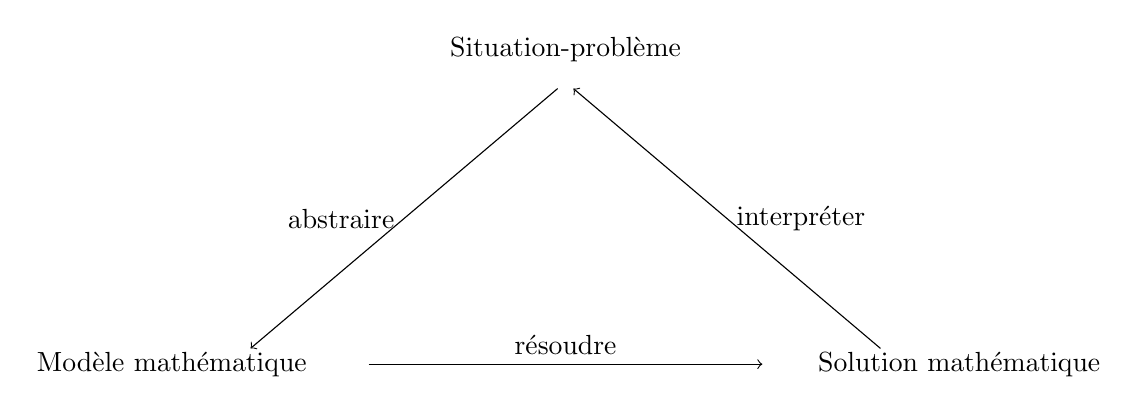
\begin{tikzpicture}
\draw (0,0) node {Situation-problème};
	\draw[->] (-0.1,-0.5) -- (-4,-3.8) node[left,pos=0.5] {abstraire};
	\draw (-5,-4) node {Modèle mathématique} ;
	\draw[->] (-2.5,-4) -- (2.5,-4) node [above, pos=0.5] {résoudre};
	\draw (5,-4)  node {Solution mathématique};
	\draw[->] (4,-3.8) -- (0.1,-0.5)  node[right,pos=0.5] {interpréter};
\end{tikzpicture}
\end{myfig}

%\begin{mywrapfigsimp}{3.05in}{3.35in}
%\noindent
%\inputpdft{1-1-fig}
%\diffypdfversion{\par\vspace*{5pt}}
%\end{mywrapfigsimp}
Comment utilise-t-on les équations différentielles en science et en génie?
On commence avec une \emph{\myindex{situation-problème}} qu'on veut comprendre.
À l'aide d'hypothèses supplémentaires pour simplifier le problème, on crée un \emph{\myindex{modèle mathématique}}.
Autrement dit, on traduit la situation en équations différentielles.
Ensuite, on utilise les mathématiques afin d'obtenir une \emph{\myindex{solution mathématique}}.
Mais ce n'est pas fini.  Il faut encore interpréter les résultats: qu'est-ce que la solution mathématique
nous dit à propos de la situation-problème de départ?

Pour ce qui est de formuler le modèle mathématique, et d'interpréter les résultats, vous ferez cela surtout dans vos cours de génie et de science.
Dans ce cours-ci, nous nous concentrerons principalement sur l'analyse mathématique.
Parfois, nous travaillerons avec des exemples réalistes simples afin de développer notre intuition et de motiver les concepts que nous verrons.

Considérons ici un exemple.  Une des équations les plus fondamentales est le \emph{\myindex{modèle de croissance exponentielle}}.
Dénotons une population de bactéries par la variable $P$ (plus précisément, $P$ dénote la quantité de population).
On suppose que l'environnement contient suffisamment de nutriments et d'espace.
Dans ce cas-là, le taux de croissance de la population de bactéries est proportionnelle à la population --
une population plus nombreuse croîtra plus rapidement.
Dénotons le temps (en secondes, disons) par la variable $t$.
0Notre modèle est alors:
\begin{equation*}
	\frac{dP}{dt} = kP,
\end{equation*}
où $k > 0$ est une constante.

\begin{example}
Supposons qu'il y a 100 bactéries au temps 0 et 200 bactéries 10 secondes plus tard.
Combien aura-t-on de bactéries à une minute (60 secondes) du début?

%mbxSTARTIGNORE
%mbxENDIGNORE
%
% Make sure to keep the above and the mbx figure below in sync!
%
D'abord, nous devons résoudre l'équation différentielle.
Nous affirmons que la fonction suivante est une solution:
\begin{equation*}
	P(t) = C e^{kt},
\end{equation*}
où $C$ est une constante.  Vérifions ceci:
\begin{equation*}
	\frac{dP}{dt} = C k e^{kt} = k P .
\end{equation*}
Il s'agit donc bel et bien d'une solution.

Ensuite?  On ne connaît pas la valeur de $C$, ni de $k$.
Mais on sait ceci: $P(0) = 100$ et $P(10) = 200$.
Substituons ces valeurs dans l'expression et regardons ce que nous obtenons:
\begin{align*}
	& 100 = P(0) = C e^{k0} = C ,\\
	& 200 = P(10) = 100 \, e^{k10} .
\end{align*}
Par conséquent, $2 = e^{10k}$ ou $\frac{\ln 2}{10} = k \approx 0,069$.
Donc:
\begin{equation*}
	P(t) = 100 \, e^{(\ln 2) t / 10} \approx 100 \, e^{0,069 t} .
\end{equation*}
À une minute, $t=60$, la population est $P(60) = 6400$.
Voir la~\figurevref{intro:plotbactfig}.
\begin{myfig}
\capstart
	\diffyincludegraphics{width=3in}{width=4.5in}{intro-plotbact}
	\caption{Croissance de bactéries en 60 secondes.\label{intro:plotbactfig}}
\end{myfig}


%mbxlatex \begin{myfig}
%mbxlatex \capstart
%mbxlatex \diffyincludegraphics{width=3in}{width=4.5in}{intro-plotbact}
%mbxlatex \caption{Bacteria growth in the first 60 seconds.\label{intro:plotbactfig}}
%mbxlatex \end{myfig}

Parlons maintenant de l'interprétation de ces résultats.
Doit-on penser qu'il y aura exactement 6400 bactéries à 60 secondes?
Bien sûr que non.
Nous avons fait des hypothèses simplificatrices qui ne seront pas exactement vraies, mais approximativement vraies.
Si nos hypothèses sont raisonnables, il y aura environ 6400 bactéries.
De plus, $P$ devrait être un nombre entier, puisqu'il compte une quantité de bactéries.
Pourtant, notre modèle admet des nombres comme $P(61) \approx 6859,35$.
%Obviously there
%are either 6859 bacteria or 6860 bacteria.
\end{example}

Habituellement, la constante $k$ dans $P' = kP$ est connue, et l'on cherche à résoudre
l'équation différentielle pour différentes \emph{conditions initiales\index{initial condition}}.
Qu'est-ce que ça veut dire?
Prenons $k=1$ pour simplifier les choses.
Supposons que nous voulons résoudre l'équation $\frac{dP}{dt} = P$
avec la condition $P(0) = 1000$ (la condition initiale).
Alors, la solution est (exercice):
\begin{equation*}
	P(t) = 1000 \, e^t .
\end{equation*}

On appelle $P(t) = C e^t$ \emph{la \myindex{solution générale}},
puisque toute solution de l'équation peut s'écrire sous cette forme pour un certain choix de la constante $C$.
La condition initiale sert à déterminer $C$, afin de trouver la
\emph{\myindex{solution particulière}}.
%Generally, when we say \myquote{particular solution,} we just mean some solution.

\subsection{Quatre équations fondamentales} \label{subsection:fourfundamental}

Quelques équations apparaissent fréquemment, et nous pouvons trouver utile de tout simplement apprendre par c{\oe}ur leur solution
(nous les verrons aussi de manière plus formelle dans les chapitres suivants).
Appelons-les nos \myindex{quatre équations fondamentales}.
Leurs solutions sont assez simples à deviner
en nous rappelant les propriétés des exponentielles, de sinus et de cosinus.
Elles sont aussi plutôt simples à vérifier, ce qu'on devrait toujours faire.
Comme ça, inutile de se demander si l'on s'est rappelé correctement de la solution.

\medskip

Voici notre première équation fondamentale:
\begin{equation*}
	\frac{dy}{dx} = k y,
\end{equation*}
où $k > 0$ est une constante.
Ici, $y$ est la variable dépendante et $x$, la variable indépendante.
La solution générale de cette équation est:
\begin{equation*}
	y(x) = C e^{kx} .
\end{equation*}
Nous avons vu ceci dans l'exemple précédent de la croissance exponentielle, même si les noms de variables ont changé.

\medskip

La deuxième équation s'obtient en modifiant légèrement la première:
\begin{equation*}
	\frac{dy}{dx} = -k y,
\end{equation*}
où $k > 0$ est une constante. La solution générale de cette équation est:
\begin{equation*}
	y(x) = C e^{-kx}.
\end{equation*}

\begin{exercise}
	Vérifiez que $y$ est bien une solution à cette équation.
\end{exercise}

Notre troisième équation fondamentale est une
\emph{\myindex{équation différentielle du second ordre}}:
\begin{equation*}
	\frac{d^2y}{{dx}^2} = -k^2 y,
\end{equation*}
où $k > 0$ est une constante. La solution générale de cette équation est:
\begin{equation*}
	y(x) = C_1 \cos(kx) + C_2 \sin(kx).
\end{equation*}
Puisque l'équation est du second ordre, la solution contient deux constantes.

\begin{exercise}
	Vérifiez que $y$ est bien une solution à cette équation.
\end{exercise}

Enfin, considérons l'équation suivante, elle aussi du second ordre:
\begin{equation*}
	\frac{d^2y}{{dx}^2} = k^2 y,
\end{equation*}
où $k > 0$ est une constante. La solution générale de cette équation est:
\begin{equation*}
	y(x) = C_1 e^{kx} + C_2 e^{-kx}
\end{equation*}
ou
\begin{equation*}
	y(x) = D_1 \cosh(kx) + D_2 \sinh(kx) .
\end{equation*}

Les fonctions $\cosh$ et $\sinh$ se définissent comme suit:
\begin{equation*}
	\cosh x = \frac{e^{x} + e^{-x}}{2} , \qquad
	\sinh x = \frac{e^{x} - e^{-x}}{2} .
\end{equation*}
Elles s'appellent respectivement \emph{\myindex{cosinus hyperbolique}}
et \emph{\myindex{sinus hyperbolique}}.
Elles sont parfois plus simples à utiliser que les fonctions exponentielles.  Elles ont de jolies propriétés, telles que
$\cosh 0 = 1$, $\sinh 0 = 0$, $\frac{d}{dx} \cosh x = \sinh x$
(non il n'y a pas de signe moins, ce n'est pas une coquille)
et $\frac{d}{dx} \sinh x = \cosh x$.

\begin{exercise}
	Vérifiez que les deux expressions sont des solutions à cette équation.
\end{exercise}

\begin{example}
	Pour les équations d'ordre supérieur, les solutions comportent plus de constantes pour lesquelles
	on doit résoudre afin d'obtenir une solution particulière.
	L'équation  $\frac{d^2y}{dx^2} = 0$ a pour solution générale $y = C_1 x + C_2$;
	il suffit d'intégrer deux fois, sans oublier les constantes d'intégration.
	Considérons les conditions initiales $y(0) = 2$ et $y'(0) = 3$.
	On substitue ces valeurs dans la solution et l'on obtient:
	\begin{equation*}
		2 = y(0) = C_1 \cdot 0 + C_2 = C_2, \qquad
		3 = y'(0) = C_1 .
	\end{equation*}
	Ainsi, $y = 3x + 2$ est la solution particulière recherchée.
\end{example}

Fait intéressant à propos de $\cosh$:  le graphe de $\cosh$ est précisément la forme d'une
chaînette pendante (pas d'une parabole, contrairement à ce qu'on pourrait croire).
Cette forme s'appelle une \emph{\myindex{caténaire}}.
De plus, le graphe de $\cosh$ offre la forme idéale pour une arche supportant son propre poids;
une telle arche de forme parabolique risquerait de s'écrouler.
Un exemple célèbre est la  {Gateway Arch} de la ville
américaine de Saint-Louis, dont la formule est inscrite dans la structure:
\begin{equation*}
	y = -127.7 \; \textrm{ft} \cdot \cosh\left( x /127.7  \; \textrm{ft} \right) + 757.7 \;\textrm{ft} .
\end{equation*}


\subsection{Exercices}

\begin{exercise}
	Montrez que $x = e^{4t}$ est une solution de $x'''-12 x'' + 48 x' - 64 x = 0$.
\end{exercise}

\begin{exercise}
	Montrez que $x = e^{t}$ n'est pas une solution de $x'''-12 x'' + 48 x' - 64 x = 0$.
\end{exercise}

\begin{exercise}
	Est-ce que $y = \sin t$ est une solution de ${\left( \frac{dy}{dt} \right)}^2 = 1 - y^2$?
	Justifiez votre réponse.
\end{exercise}

\begin{exercise}
	Considérons $y'' + 2y' - 8y = 0$.
	Essayez une solution de la forme $y = e^{rx}$ pour une constante (à déterminer) $r$.
	Existe-il une valeur de $r$ qui donne une solution? Si oui, trouvez toutes les valeurs possibles de $r$.
\end{exercise}

\begin{exercise}
	Vérifiez que $x = C e^{-2t}$ est une solution de $x' = -2x$.
	Trouvez $C$ satisfaisant à la condition initiale $x(0) = 100$.
\end{exercise}

\begin{exercise}
	Vérifiez que $x = C_1 e^{-t} + C_2 e^{2t}$ est une solution de $x'' - x' -2 x =	0$.
	Trouvez $C_1$ et $C_2$ satisfaisant aux conditions initiales $x(0) = 10$
	et $x'(0) = 0$.
\end{exercise}

\begin{exercise}
	Trouvez une solution
	${(x')}^2 + x^2 = 4$
	en utilisant ce que vous avez appris à propos des dérivées dans vos cours de calcul.
\end{exercise}

\begin{exercise}
	Résolvez
	\begin{tasks}(2)
		\task $\dfrac{dA}{dt} = -10 A, \quad A(0)=5$
		\task $\dfrac{dH}{dx} = 3 H, \quad H(0)=1$
		\task $\dfrac{d^2y}{dx^2} = 4 y, \quad y(0)=0, \quad y'(0)=1$
		\task $\dfrac{d^2x}{dy^2} = -9 x, \quad x(0)=1, \quad x'(0)=0$
	\end{tasks}
\end{exercise}

\begin{exercise}
	Existe-t-il une solution de $y' = y$, telle que $y(0) = y(1)$?
\end{exercise}

\begin{exercise}
	La population de la ville X était 100~000 il y a 20 ans, et 120~000 il y a 10 ans.  
	Si l'on suppose une croissance continue, on peut utiliser le modèle de croissance exponentielle
	(comme pour une population de bactéries). À combien estimez-vous la population actuelle maintenant?
\end{exercise}

\begin{exercise}
	Supposons qu'un coach de football obtient présentement un salaire annuel de 1 million $\$$,
	et qu'il a une augmentation salariale de $10\%$ chaque année (donc modèle de croissance exponentielle, comme les bactéries).
	Dénotons par $s$ le salaire en millions de dollars, et $t$ le temps en années.
	\begin{tasks}(2)
	\task Trouvez $s(0)$ et $s(1)$.
	\task Après combien d'années approximativement le salaire sera-t-il de 10 millions?
	\task Après combien d'années approximativement le salaire sera-t-il de 20 millions?
	\task Après combien d'années approximativement le salaire sera-t-il de 30 millions?
	\end{tasks}
\end{exercise}


%mbxSTARTIGNORE
\noindent
\emph{Note: Les exercices dont les numéros sont 101 et plus ont des réponses à la fin du manuel.}
%mbxENDIGNORE

%mbx <p><em>Note: Exercises with numbers 101 and higher have solutions.</em></p>

\setcounter{exercise}{100}

\begin{exercise}
	Montrez que $x = e^{-2t}$ est une solution de $x'' + 4x' + 4x = 0$.
\end{exercise}
\exsol{%
	Calculer $x' = -2e^{-2t}$ et $x'' = 4e^{-2t}$.  Alors, 
	$(4e^{-2t}) + 4 (-2e^{-2t}) + 4 (e^{-2t}) = 0$.
}

\begin{exercise}
	Est-ce que $y = x^2$ est une solution de $x^2y'' - 2y = 0$?  Justifiez votre réponse.
\end{exercise}
\exsol{%
	Oui.
}

\begin{exercise}
	Soit $xy'' - y' = 0$.  Essayez une solution de la forme $y = x^r$.
	Existe-t-il une valeur de $r$ qui donne une solution?
	Si oui, trouvez toutes les valeurs possibles de $r$.
\end{exercise}
\exsol{%
	$y=x^r$ est une solution pour $r=0$ et $r=2$.
}


\begin{exercise}
	Vérifiez que $x=C_1e^t+C_2$ est une solution de $x''-x' = 0$.
	Trouvez $C_1$ et $C_2$ telles que $x(0) = 10$ et $x'(0) = 100$.
\end{exercise}
\exsol{%
	$C_1 = 100$, $C_2 = -90$
}

\begin{exercise}
	Résolvez $\frac{d\varphi}{ds} = 8 \varphi$ et $\varphi(0) = -9$.
\end{exercise}
\exsol{%
	$\varphi = -9 e^{8s}$
}

\begin{exercise}
	Résolvez
	\begin{tasks}(2)
	\task $\dfrac{dx}{dt} = -4x, \quad x(0)=9$
	\task $\dfrac{d^2x}{dt^2} = -4x, \quad x(0)=1, \quad x'(0)=2$
	\task $\dfrac{dp}{dq} = 3 p, \quad p(0)=4$
	\task $\dfrac{d^2T}{dx^2} = 4 T, \quad T(0)=0, \quad T'(0)=6$
	\end{tasks}
\end{exercise}
\exsol{%
	a)~$x=9e^{-4t}$ \quad
	b)~$x=\cos(2t)+\sin(2t)$ \quad
	c)~$p=4e^{3q}$ \quad
	d)~$T=3\sinh(2x)$
}

%%%%%%%%%%%%%%%%%%%%%%%%%%%%%%%%%%%%%%%%%%%%%%%%%%%%%%%%%%%%%%%%%%%%%%%%%%%%%%

\sectionnewpage
\section{Classification des équations différentielles}
\label{classification:section}

%%Perhaps no [EP] ref?
%\sectionnotes{less than 1 lecture or left as reading\BDref{, \S1.3 in \cite{BD}}}
Il y a plusieurs types d'équations différentielles, et on les classifie en différentes catégories selon leurs propriétés.
Parlons brièvement d'une classification de base.  D'abord, la distinction entre EDO et EDP:
\begin{itemize}
\item
	Dans les \emph{équations différentielles ordinaires}\index{Équations différentielles ordinaires}\index{EDO}, ou EDO,
	les dérivées sont prises par rapport à une seule variable.  Autrement dit, il y a une seule variable indépendante.

\item
	Dans les \emph{équations aux dérivées partielles}\index{Équations aux dérivées partielles}\index{EDP}, ou EDP,
	les dérivées sont prises par rapport à plusieurs variables.  Autrement dit, il y a plusieurs variables indépendantes.
\end{itemize}

Voici quelques exemples d'équations différentielles ordinaires:
\begin{align*}
	& \frac{d y}{dt} = ky  & & \text{(croissance exponentielle\index{exponential growth})} \\
	& \frac{d y}{dt} = k(A-y)  & & \text{(\myindex{loi de refroidissement de Newton})} \\
	& m \frac{d^2 x}{dt^2} + c \frac{dx}{dt} + kx = f(t) . & &
\text{(vibrations mécaniques\index{mechanical vibrations})}
\end{align*}
Voici quelques exemples d'équations aux dérivées partielles:
\begin{align*}
	& \frac{\partial y}{\partial t} + c \frac{\partial y}{\partial x} = 0 & &
		\text{(équation du transport\index{Équation du transport})} \\
	& \frac{\partial u}{\partial t} = \frac{\partial^2 u}{\partial x^2}  & &
		\text{(équation de la chaleur ou de la diffusion\index{Équation de la chaleur/diffusion})} \\
	& \frac{\partial^2 u}{\partial t^2} = \frac{\partial^2 u}{\partial x^2} + \frac{\partial^2 u}{\partial y^2} . & &
		\text{(équation de l'onde en 2 dimensions\index{Équation de l'onde en deux dimensions})}
\end{align*}

Lorsque la situation est soumise à plusieurs équations en même temps, on a un
\emph{\myindex{système d'équations différentielles}}.
Par exemple:
\begin{equation*}
	y' = x , \qquad x' = y
\end{equation*}
est un système simple d'équations différentielles ordinaires.
Les \myindex{équations de Maxwell} en électromagnétisme forment elles aussi un système d'équations aux dérivées partielles:
\begin{align*}
	& \nabla \cdot \vec{D} = \rho & & \nabla \cdot \vec{B} = 0  \\
	& \nabla \times \vec{E} = - \frac{\partial \vec{B}}{\partial t} &
	& \nabla \times \vec{H} = \vec{J} + \frac{\partial \vec{D}}{\partial t} .
\end{align*}
Les opérateurs de divergence $\nabla \cdot$ et de rotationnel $\nabla \times$
s'écrivent en termes de dérivées partielles des fonctions en termes des variables $x$, $y$ et $z$ .

\medskip

Le prochain élément d'information est l'\emph{\myindex{ordre}} de l'équation (ou du système).
L'ordre est tout simplement l'ordre de la plus grande dérivée apparaissant dans l'équation.
Si la plus grande dérivée est la dérivée première, c'est une équation du premier ordre.
Si la dérivée la plus grande est la dérivée seconde, alors c'est une équation du deuxième ordre.
Par exemple, la loi de refroidissement de Newton est une équation du premier ordre,
alors que l'équation des vibrations mécaniques est une équation du deuxième ordre.
L'équation décrivant les vibrations transversales dans une poutre,
\begin{equation*}
	a^4 \frac{\partial^4 y}{\partial x^4} + \frac{\partial^2 y}{\partial t^2} = 0,
\end{equation*}
est une équation aux dérivées partielles d'ordre quatre.
En effet, une des dérivées dans l'équation est la quatrième dérivée.
Le fait que la dérivée en $t$ soit seulement d'ordre deux n'affecte pas l'ordre de l'équation.

Dans le premier chapitre, nous commencerons par les équations différentielles ordinaires du premier ordre,
c'est-à-dire les équations de la forme $\frac{dy}{dx} = f(x,y)$.
En général, les équations de petit ordre sont plus simples à résoudre et à étudier.

\medskip

Dans la classification des équations, on s'intéresse aussi à comment les variables dépendantes
apparaissent dans l'équation (ou le système).
En particulier, on l'appelle une \emph{équation linéaire}\index{linear equation}
si la variable dépendante (ou les variables dépendantes) et ses dérivées apparaissent linéairement,
c'est-à-dire qu'elles ne sont pas multipliées ensemble et qu'aucune autre fonction des variables dépendantes n'apparaît dans l'équation.
Sinon, il s'agit d'une équation \emph{non linéaire}\index{nonlinear equation}.
Une EDO est linéaire si elle peut être exprimée de la manière suivante:
\begin{equation} \label{classification:eqlingen}
a_n(x) \frac{d^n y}{dx^n}
	+ a_{n-1}(x) \frac{d^{n-1} y}{dx^{n-1}}
	+ \cdots
	+ a_{1}(x) \frac{dy}{dx}
	+ a_{0}(x) y
	= b(x) *.
\end{equation}
Les fonctions $a_0$, $a_1$, \ldots, $a_n$ s'appellent les \emph{\myindex{coefficients}}.
L'équation peut dépendre arbitrairement de la variable indépendante.
Ainsi, l'équation suivante est linéaire:
\begin{equation} \label{classification:eqlinex}
	e^x \frac{d^2 y}{dx^2} + \sin(x) \frac{d y}{dx} +  x^2 y = \frac{1}{x},
\end{equation}
et ce, malgré la présence de $e^x$ et de $\sin(x)$, puisque $y$ et ses dérivées apparaissent de manière linéaire dans l'équation.

Tous les exemples mentionnés au début de la section sont linéaires.
Ce n'est peut-être pas évident dans le cas des équations de Maxwell;
pour s'en convaincre, on peut écrire la divergence et le rotationnel en termes des dérivées partielles.

Considérons maintenant quelques équations non linéaires.
Par exemple, l'équation de \myindex{Burger},
\begin{equation*}
	\frac{\partial y}{\partial t} +  \frac{\partial y}{\partial x}
	= \nu \frac{\partial^2 y}{\partial x^2},
\end{equation*}
est une EDP du second ordre, qui est non linéaire, puisque $y$ et $\frac{\partial y}{\partial x}$ sont multipliés ensemble.
L'équation suivante:
\begin{equation} \label{classification:eqnonlinode}
	\frac{dx}{dt} = x^2,
\end{equation}
est une EDO non linéaire du premier ordre, puisque la variable dépendante $x$ est au carré.

\medskip

Une équation qui est linéaire est de plus appelée \emph{\myindex{homogène}}
si tous les termes dépendent de la variable dépendante.
Autrement dit, il n'y a aucun terme qui dépend uniquement de la variable indépendante.
Sinon, l'équation est dite \emph{\myindex{non homogène}}.
Par exemple, l'équation de la croissance exponentielle, l'équation de l'onde et l'équation du transport sont homogènes.
L'équation des vibrations mécaniques est non homogène à moins que $f(t)$ soit la fonction nulle.
De manière analogue, la loi de refroidissement de Newton est non homogène sauf si la température ambiante $A$ est nulle.
Une EDO linéaire homogène peut être écrite sous la forme suivante:
\begin{equation*}
a_n(x) \frac{d^n y}{dx^n}
	+ a_{n-1}(x) \frac{d^{n-1} y}{dx^{n-1}}
	+ \cdots
	+ a_{1}(x) \frac{dy}{dx}
	+ a_{0}(x) y = 0 .
\end{equation*}
Comparez à \eqref{classification:eqlingen} et observez l'absence de fonction $b(x)$.

\medskip

Lorsque les coefficients d'une équation linéaire sont en fait des constantes,
on dit alors que l'équation est à \emph{coefficients constants}\index{constant coefficient}.
Les coefficients sont les fonctions multipliées par la variable dépendante ou par une de ses dérivées,
et non la fonction $b(x)$ qui apparaît seule.
Une EDO non homogène à coefficients constants a la forme suivante:
\begin{equation*}
	a_n \frac{d^n y}{dx^n}
		+ a_{n-1} \frac{d^{n-1} y}{dx^{n-1}}
		+ \cdots
		+ a_{1} \frac{dy}{dx}
		+ a_{0} y
		= b(x),
\end{equation*}
où $a_0, a_1, \ldots, a_n$ sont toutes des constantes, mais où
$b$ peut dépendre de la variable indépendante $x$.
L'équation des vibrations mécaniques que nous avons vue plus haut est une
EDO non homogène du second ordre à coefficients constants.

La même nomenclature s'applique aux EDP.
Par conséquent, les équations du transport, de la chaleur/diffusion et
de l'onde sont toutes des EDP linéaires à coefficients constants.

\medskip

Pour terminer, une équation est dite \emph{\myindex{autonome}}
 si l'équation ne dépend pas de la variable indépendante.
 Pour des EDO autonomes, on pensera souvent à la variable indépendante comme à la variable du temps.
 Être une équation autonome signifie que l'équation ne varie pas dans le temps.
 Par exemple, la loi de refroidissement de Newton est autonome, ainsi que l'équation \eqref{classification:eqnonlinode}.
 Par contre, les équations de vibrations mécaniques ou \eqref{classification:eqlinex} ne sont pas autonomes.

\subsection{Exercices}

\begin{exercise}
	Classifiez les équations suivantes. S'agit-il d'une EDO ou d'une EDP?
	Est-ce une équation ou un système?  Quel est l'ordre?
	Est-ce linéaire ou non-linéaire et si c'est linéaire, est-ce homogène?
	à coefficients constants?  Si c'est une EDO, est-elle autonome?
	\begin{tasks}(2)
	\task $\displaystyle \sin(t) \frac{d^2 x}{dt^2} + \cos(t) x = t^2$
	\task $\displaystyle \frac{\partial u}{\partial x} + 3 \frac{\partial u}{\partial y} = xy$
	\task $\displaystyle y''+3y+5x=0, \quad x''+x-y=0$
	\task $\displaystyle \frac{\partial^2 u}{\partial t^2} + u\frac{\partial^2 u}{\partial s^2} = 0$
	\task $\displaystyle x''+tx^2=t$
	\task $\displaystyle \frac{d^4 x}{dt^4} = 0$
	\end{tasks}
\end{exercise}

\begin{exercise}
Si $\vec{u} = (u_1,u_2,u_3)$ est un vecteur, sa divergence est:
$\nabla \cdot \vec{u} =
	\frac{\partial u_1}{\partial x}
	+ \frac{\partial u_2}{\partial y}
	+ \frac{\partial u_3}{\partial z}$ et son rotationnel est:
	$\nabla \times \vec{u} =
		\Bigl(	\frac{\partial u_3}{\partial y} - \frac{\partial u_2}{\partial z} , ~
				\frac{\partial u_1}{\partial z} - \frac{\partial u_3}{\partial x} , ~
				\frac{\partial u_2}{\partial x} - \frac{\partial u_1}{\partial y} \Bigr)$.
Observez que le rotationnel d'un vecteur est lui-même un vecteur.
écrivez les équations de Maxwell en termes de dérivées partielles et classifiez le système.
\end{exercise}

\begin{exercise}
	Supposons que $F$ est une fonction linéaire, c'est-à-dire que $F(x,y) = ax+by$
	pour des constantes $a$ et $b$.  Classifiez les équations de la forme $F(y',y) = 0$.
\end{exercise}

\begin{exercise}
	Trouvez un exemple explicite d'un système de deux EDO satisfaisant aux critères suivants:
	d'ordre trois, non autonome, non homogène, dont les coefficients sont non constants,
	et tel que toutes les dérivées possibles apparaissent dans le système au moins une fois.
\end{exercise}

\setcounter{exercise}{100}

\begin{exercise}
	Classifiez les équations suivantes. S'agit-il d'une EDO ou d'une EDP?
	Est-ce une équation ou un système?  Quel est l'ordre?
	Est-ce linéaire ou non-linéaire et si c'est linéaire, est-ce homogène?
	À coefficients constants?
	Si c'est une EDO, est-elle autonome?
	\begin{tasks}(2)
	\task $\displaystyle \frac{\partial^2 v}{\partial x^2} + 3 \frac{\partial^2 v}{\partial y^2} = \sin(x)$
	\task $\displaystyle \frac{d x}{dt} + \cos(t) x = t^2+t+1$
	\task $\displaystyle \frac{d^7 F}{dx^7} = 3F(x)$
	\task $\displaystyle y''+8y'=1$
	\task $\displaystyle x''+tyx'=0, \quad y''+txy = 0$
	\task $\displaystyle \frac{\partial u}{\partial t} = \frac{\partial^2 u}{\partial s^2} + u^2$
	\end{tasks}
\end{exercise}
\exsol{%
	a) EDP\@, équation, deuxième ordre, linéaire, non homogène, coefficients constants. \\
	b) EDO\@, équation, premier ordre, linéaire, non homogène, coefficients non constants, non autonome.\\
	c) EDO\@, équation, ordre sept, linéaire, homogène, coefficients constants, autonome.\\
	d) EDO\@, équation, deuxième ordre, linéaire, non homogène, coefficients constants, autonome.\\
	e) EDO\@, système, deuxième ordre, non linéaire.\\
	f) EDP\@, équation,  deuxième ordre, non linéaire.
}

\begin{exercise}
	Écrivez la forme générale de l'équation différentielle ordinaire d'ordre \emph{zero} et linéaire.
	Trouvez sa solution générale.
\end{exercise}
\exsol{%
	équation: $a(x) y = b(x)$, solution: $y = \frac{b(x)}{a(x)}$.
}

\begin{exercise}
	Pour quelles valeurs de $k$ l'équation $\frac{dx}{dt}+x^k = t^{k+2}$ est-elle linéaire?
	Indice: il y a deux valeurs possibles.
\end{exercise}
\exsol{%
	$k=0$ ou $k=1$
}
 %\input ch-intro-fr.tex


%%%%%%%%%%%%%%%%%%%%%%%%%%%%%%%%%%%%%%%%%%%%%%%%%%%%%%%%%%%%%%%%%%%%%%%%%%%%%%

% First order ODEs chapter
% Traduction du chapitre 1
% Première version : Août 2020
\chapter{Équations du premier ordre} \label{fo:chapter}

%%%%%%%%%%%%%%%%%%%%%%%%%%%%%%%%%%%%%%%%%%%%%%%%%%%%%%%%%%%%%%%%%%%%%%%%%%%%%%

\section{Intégrales en tant que solutions}
\label{integralsols:section}

%\sectionnotes{1 lecture (or less)\EPref{, \S1.2 in \cite{EP}}\BDref{,
%covered in \S1.2 and \S2.1 in \cite{BD}}}

Une équation différentielle du premier ordre est une équation pouvant s'écrire de la forme suivante:
\begin{equation*}
	\frac{dy}{dx} = f(x,y)
\end{equation*}
ou
\begin{equation*}
	y' = f(x,y) .
\end{equation*}
Il n'y a pas de méthode générale simple pour trouver la solution  à toute équation du premier ordre.
Nous verrons quelques cas où c'est possible.
Commençons par supposer que $f$ est une fonction de $x$, seulement, c'est-à-dire:
\begin{equation} \label{ias:inteq}
	y' = f(x) .
\end{equation}
On peut alors intégrer des deux côtés pour trouver une solution:
\begin{equation*}
	\int y'(x) \,dx = \int f(x) \,dx + C ,
\end{equation*}
c'est-à-dire
\begin{equation*}
	y(x) = \int f(x) \,dx + C .
\end{equation*}
Dans ce cas-ci, la solution générale, $y(x)$, est en fait une primitive de $f(x)$,
à laquelle on ajoute la constante d'intégration.

\medskip

Prenons ce moment pour aborder un point délicat du vocabulaire de calcul.
Souvent, quand on pense aux intégrales, on pense à une \myindex{intégrale indéfinie}.
En réalité, une intégrale indéfinie est une \emph{\myindex{primitive}} ou, plus précisément, une famille de primitives.
Ce sont les intégrales définies (les intégrales avec des bornes) qui sont les vraies intégrales.
Mais c'est pratique de parler d'intégrale \og{}indéfinie\fg{} puisqu'on peut toujours écrire l'intégrale indéfinie
$\int f(x) \,dx + C$ comme suit, grâce au théorème fondamental du calcul:
\begin{equation*}
	\int_{x_0}^x f(t) \,dt + C .
\end{equation*}
C'est ce qui nous permet de dire  \emph{ \myindex{intégrer}} quand, en réalité,
on veut dire  \emph{trouver la \myindex{primitive}}.

L'intégration est tout simplement un moyen parmi d'autres pour calculer une primitive
(moyen qui fonctionne toujours, comme on le verra dans les exemples suivants).
Mais on définit l'intégrale comme étant l'aire sous la courbe.
Pour simplifier les choses, nous continuerons d'utiliser la notation intégrale pour écrire une primitive,
et \emph{gardez toujours en tête} comment réécrire l'intégrale indéfinie comme une intégrale définie.

\begin{example}
	Trouvons la solution générale de $y' = 3 x^2$.

	En intégrant des deux côtés, on trouve $y = x^3 + C$.  Vérifions notre solution en prenant sa dérivée :
	$y' = 3x^2$.  C'est \emph{précisément} notre équation.
\end{example}

Normalement, on a aussi une {\em condition initiale}, de la forme $y(x_0) = y_0$, où $x_0,y_0$ sont des nombre réels (habituellement, $x_0=0$, mais ce n'est pas toujours le cas).
Dans ce cas, la solution s'écrit très bien sous forme intégrale.
Supposons que le problème à résoudre est $y' = f(x)$, $y(x_0) = y_0$. Alors, la solution est:
%
\begin{equation} \label{int:eqdef}
	y(x) = \int_{x_0}^x f(s) \,ds + y_0 .
\end{equation}
Vérifions.  Par le théorème fondamental du calcul, la dérivée de l'intégrale précédente est $f(x)$,
et donc $y(x)$ est bel et bien est une solution à l'équation différentielle.
Maintenant, vérifions qu'elle satisfait aussi à la condition initiale:
\begin{equation*}
	y(x_0) = \int_{x_0}^{x_0} f(x)\,dx + y_0 = y_0.
\end{equation*}
Ainsi, la condition initiale est également vérifiée par l'équation~\eqref{int:eqdef}.

Gardez en tête qu'une intégrale définie et une intégrale indéfinie sont deux choses très différentes.
La valeur d'une intégrale définie est toujours un nombre.
Par conséquent, \eqref{int:eqdef} est une formule qu'on peut utiliser pour obtenir n'importe quelle valeur spécifique de la solution.
C'est une fonction comme une autre.  Il n'est pas toujours possible ni nécessaire de trouver une formule analytique pour la primitive.

%can plug into the calculator or a computer, and it will be happy to calculate
%specific values for us.  We will easily be able to plot the
%solution and work with it just like with any other function.
%It is not so crucial to always find a
%closed form for the antiderivative.

\begin{example}
	Résolvons
	\begin{equation*}
		y' = e^{-x^2}, \qquad y(0) = 1 .
	\end{equation*}

	Par la solution précédente, la solution doit être:
	\begin{equation*}
		y(x) = \int_0^x e^{-s^2} \,ds + 1 .
	\end{equation*}
	Or, il n'y a pas de formule plus explicite pour la primitive de $e^{-x^2}$
	(on ne peut pas, par exemple, faire un changement de variables...).
	Et la solution sous forme intégrale est très correcte, telle quelle.
	Elle joue un rôle important, d'ailleurs, en statistique.
\end{example}

La méthode de l'intégrale sert aussi à résoudre des équations de la forme suivante:
\begin{equation*}
	y' = f(y) .
\end{equation*}
Écrivons cette équation dans la \myindex{notation de Leibniz}:
\begin{equation*}
	\frac{dy}{dx} = f(y) .
\end{equation*}
Le théorème de la fonction inverse, en calcul, nous permet d'échanger les rôles de $x$ et de $y$ pour écrire l'équation sous la forme suivante:
\begin{equation*}
	\frac{dx}{dy} = \frac{1}{f(y)} .
\end{equation*}
On dirait qu'on fait tout simplement des manipulations algébriques avec $dx$ et $dy$, qu'on traite comme des nombres.
Et c'est vrai que ça marche.
Mais attention! Lorsqu'on verra des équations aux dérivées partielles, ce type de raisonnement ne fonctionnera plus.

Dans le cas présent, on peut intégrer l'équation précédente des deux côtés pour obtenir:
\begin{equation*}
	x(y) = \int \frac{1}{f(y)} \,dy + C .
\end{equation*}
On peut ensuite tenter de résoudre pour $y$.  Voyons quelques exemples de ceci.

\begin{example}
	Plus haut, nous avons résolu l'équation $y' = ky$ (pour $k > 0$) en devinant que c'était
	$y=Ce^{kx}$.  Reprenons cet exemple de manière plus systématique.

	Observons d'abord que  $y=0$ est une solution.  Supposons donc dorénavant que $y\not= 0$.
	On peut alors écrire:
	\begin{equation*}
		\frac{dx}{dy} = \frac{1}{ky} .
	\end{equation*}
	On intègre des deux côtés pour obtenir :
	\begin{equation*}
		x(y) = x = \frac{1}{k} \ln \, \lvert y\rvert  + D,
	\end{equation*}
	où $D$ est une constante arbitraire.
	Maintenant, on résout pour $y$ ou, plus précisément, pour $\lvert y \rvert$:
	\begin{equation*}
		\lvert y \rvert = e^{kx-kD} =  e^{-kD} e^{k x} .
	\end{equation*}
	Puisque $e^{-kD}$ est une constante positive arbitraire, on peut la remplacer par une constante arbitraire $C$;
	ici, $C$ peut aussi prendre la valeur 0 (incorporant ainsi la solution $y=0$) ou des valeurs négatives,
	ce qui nous permet de nous débarasser de la valeur absolue.  On obtient alors la solution générale devinée plus tôt, $y = Ce^{kx}$.
\end{example}

\begin{example}
	Trouvons la solution générale de $y' = y^2$.

	Notons d'abord que $y=0$ est une solution.  Nous supposerons dorénavant que $y \not= 0$.
	Écrivons
	\begin{equation*}
		\frac{dx}{dy} = \frac{1}{y^2} .
	\end{equation*}
	On intègre pour obtenir
	\begin{equation*}
		x = \frac{-1}{y} + C .
	\end{equation*}
	On résout pour $y$:
	\begin{equation*}
		y = \frac{1}{C-x}.
	\end{equation*}
	La solution générale est donc
	\begin{equation*}
		y = \frac{1}{C-x} \qquad \text{ou} \qquad y = 0.
	\end{equation*}
	Cette solution comporte des singularités.
	Par exemple, si $C=1$, alors la solution \og{}explose\fg{} lorsqu'on s'approche de $x=1$.
	Voir la~\figureref{1over1mx:fig}.
	En général, c'est difficile de prédire le comportement d'une solution juste en regardant l'équation différentielle.
	En effet, l'équation $y' = y^2$ est très jolie et définie partout, mais sa solution est seulement définie sur un intervalle $(-\infty, C)$ ou
	$(C, \infty)$.  Dans une telle situation, on retient seulement une de ces deux solutions, dépendamment de la condition initiale.
	Si, par exemple, on a pour condition initiale $y(0) = 1$, alors la solution est $y=\frac{1}{1-x}$,
	et cette solution est seulement définie sur l'intervalle  $(-\infty,1)$.
	Dans la figure, c'est la partie gauche du graphe.

	\begin{myfig}
		\capstart
		\diffyincludegraphics{width=3in}{width=4.5in}{1over1mx}
		\caption{Graphe de $y=\frac{1}{1-x}$.\label{1over1mx:fig}}
	\end{myfig}
\end{example}

Parmi les problèmes classiques menant à des équations différentielles résolubles par intégration,
on retrouve les problèmes de \myindex{vitesse},
d'\myindex{accélération} et de  \myindex{distance}.
Vous avez probablement vu de tels problèmes dans vos cours de calcul.

\begin{example}
	Supposons qu'une voiture roule à une vitesse de $e^{t/2}$ mètres par seconde,
	où $t$ est le temps mesuré en secondes.
	Quelle distance a-t-elle parcourue en 2 secondes (si elle commence à $t=0$)?
	En 10 secondes?

	Dénotons par $x$ la distance parcourue par la voiture.
	L'équation à résoudre est:
	\begin{equation*}
		x' = e^{t/2} .
	\end{equation*}
	On intègre cette équation pour obtenir :
	\begin{equation*}
		x(t) = 2 e^{t/2} + C .
	\end{equation*}
	Il nous reste à déterminer $C$.  On sait qu'à $t=0$,
	$x=0$.  Autrement dit, $x(0) = 0$.  Donc:
	\begin{equation*}
		0 = x(0) = 2e^{0/2} + C = 2 + C .
	\end{equation*}
	Ainsi, $C = -2$, et
	\begin{equation*}
		x(t) = 2 e^{t/2} - 2 .
	\end{equation*}
	Il nous suffit de substituer $t=2$ et $t=10$ pour obtenir la distance parcourue après 2 et 10 secondes.
	\begin{equation*}
		x(2) = 2e^{2/2} - 2 \approx 3{,}44 \text{ mètres} ,
		\qquad
		x(10) = 2e^{10/2} - 2 \approx 294 \text{ mètres} .
	\end{equation*}
\end{example}

\begin{example}
	Supposons que la voiture accélère à $\unitfrac[t^2]{m}{s^2}$.
	À $t=0$, la voiture est au mètre 1 et roule à une vitesse de \unitfrac[10]{m}{s}.
	Où est la voiture à $t=10$?

	Ceci est en fait un problème du deuxième ordre, puisque l'accélération est la dérivée seconde de la fonction de position.
	Dénotons par $x$ la distance parcourue, alors $x'$ est la vitesse, et $x''$, l'accélération.
	Ceci nous donne l'équation différentielle avec conditions initiales suivante:
	\begin{equation*}
		x'' = t^2 , \qquad x(0) = 1 , \qquad x'(0) = 10 .
	\end{equation*}
	Posons $x' = v$.  Le problème devient alors
	\begin{equation*}
		v' = t^2, \qquad v(0) = 10 .
	\end{equation*}
	On peut résoudre pour $v$ et ensuite intégrer $v$ pour trouver $x$.
\end{example}

\begin{exercise}
	Résolvez pour $v$ et ensuite pour $x$.  Trouvez $x(10)$ pour répondre à la question.
\end{exercise}


\subsection{Exercices}

\begin{exercise}
	Résolvez$\frac{dy}{dx} = x^2+x$, $y(1)=3$.
\end{exercise}

\begin{exercise}
	Résolvez $\frac{dy}{dx} = \sin (5x)$, $y(0)=2$.
\end{exercise}

\begin{exercise}
	Résolvez $\frac{dy}{dx} = \frac{1}{x^2-1}$, $y(0)=0$.
\end{exercise}

\begin{exercise}
	Résolvez $y' = y^3$, $y(0)=1$.
\end{exercise}

\begin{exercise}[un peu plus difficile]
	Résolvez $y' = (y-1)(y+1)$, $y(0)=3$.
\end{exercise}

\begin{exercise}
	Résolvez $\frac{dy}{dx} = \frac{1}{y+1}$, $y(0)=0$.
\end{exercise}

\begin{exercise}[plus difficile]
	Résolvez $y'' = \sin x$, $y(0)=0$, $y'(0) = 2$.
\end{exercise}

\begin{exercise}
	Une fusée se déplace à une vitesse de \unitfrac[$2t^2+1$]{km}{s} ($t$ est mesuré en secondes).
	La terre est directement derrière la fusée et à $t=0$, elle est à 1000 kilomètres de la terre.  À quelle distance se trouve la fusée 1 minute plus tard?
\end{exercise}

\begin{exercise}
	Résolvez $\frac{dx}{dt} = \sin(t^2)+t$, $x(0)=20$.  Vous pouvez laisser votre réponse sous forme d'intégrale définie.
\end{exercise}

\begin{exercise}
	Une balle tombe avec une accélération constante de $9,8$ mètres par seconde au carré.
	Écrivez l'équation différentielle pour la hauteur $h$ en mètres.
	Ensuite, en supposant que $h(0) = 100$ mètres, calculez le temps qu'il faudra à la balle pour toucher au sol.
\end{exercise}

\begin{exercise}
	Trouvez la solution générale de $y' = e^x$,  et ensuite $y' = e^y$.
\end{exercise}


\setcounter{exercise}{100}

\begin{exercise}
	Résolvez $\frac{dy}{dx} = e^x + x$, $y(0) = 10$.
\end{exercise}
\exsol{%
	$y = e^x + \frac{x^2}{2} + 9$
}

\begin{exercise}
	Résolvez $x' = \frac{1}{x^2}$, $x(1)=1$.
\end{exercise}
\exsol{%
	$x = {(3t-2)}^{1/3}$
}

\begin{exercise}
	Résolvez $x' = \frac{1}{\cos(x)}$, $x(0)=\frac{\pi}{2}$.
\end{exercise}
\exsol{%
	$x = \sin^{-1} \bigl(t+1\bigr)$
}

\begin{exercise}
	Max est dans une voiture partant de Québec et filant à $10t+70$ kilomètres par heure,où $t$est mesuré en heures.
	À $t=0$, Max est à 10 kilomètres de Québec.  À quelle distance de Québec sera Max deux heures plus tard?
\end{exercise}
\exsol{%
	170
}

\begin{exercise}
	Résolvez $y' = y^n$, $y(0) = 1$, où $n$ est un entier positif.
	Indice: il y a plusieurs cas à considérer.
\end{exercise}
\exsol{%
	Si $n \not= 1$, alors $y={\bigl((1-n)x+1\bigr)}^{1/(1-n)}$.
	Si $n=1$, alors $y = e^x$.
}

\begin{exercise}
	Une boule de neige fond; le taux de variation du volume de la boule est proportionnelle à sa surface.
	Si le rayon de la boule est $r$ centimètres, son volume est $\nicefrac{4}{3}\,\pi r^3$ centimètres cube
	et la surface est$4 \pi r^2$ centimètres carré.
	Trouvez l'équation différentielle décrivant la variation de $r$.
	Ensuite, supposons qu'à $t=0$ minutes, le rayon est de 10 centimètres et qu'après 5 minutes, le rayon est de 8 centimètres.
	Dans combien de temps est-ce que la boule de neige aura complètement fondu?
	%Set up the differential equation for how $r$ is changing.
	%Then, suppose that at time $t=0$ minutes, the radius is 10 centimeters.
	%After 5 minutes, the radius is 8 centimeters.  At what time $t$ will the
	%snowball be completely melted?
\end{exercise}
\exsol{%
	L'équation est $r' = -C$, où $C$ est une constante.
	La boule de neige aura complètement fondu 25 minutes après $t=0$.
}

\begin{exercise}
	Trouvez la solution générale à $y''''= 0$.  Combien de constantes distinctes sont nécessaires?
\end{exercise}
\exsol{%
	$y = Ax^3 + Bx^2 + Cx + D$, donc quatre constantes.
}

%%%%%%%%%%%%%%%%%%%%%%%%%%%%%%%%%%%%%%%%%%%%%%%%%%%%%%%%%%%%%%%%%%%%%%%%%%%%%%

\sectionnewpage
\section{Champs de direction}
\label{slopefields:section}

%\sectionnotes{1 lecture\EPref{, \S1.3 in \cite{EP}}\BDref{,
%\S1.1 in \cite{BD}}}

%At this point it may be good to first try the
%Lab I\index{IODE software!Lab I} and/or Project I\index{IODE software!Project I} from the
%IODE website: \url{http://www.math.uiuc.edu/iode/}.
%
%\medskip

Rappelons que l'équation générale du premier ordre s'écrit comme suit :
\begin{equation*}
	y' = f(x , y).
\end{equation*}
Souvent, on ne peut tout simplement pas trouver une solution analytique à cette équation.
Mais on aimerait au moins avoir une idée de la forme et du comportement de la solution, ou trouver une solution approximative.



\subsection{Champs de direction}

%As you have seen in IODE Lab I (if you did it),
L'équation $y' = f(x , y)$ donne une formule pour la pente de la tangente à une solution à chaque point du plan $(x , y)$.
Autrement dit, si $y(x)$ est une solution, alors son graphe passe par le point $(x , y)$,
et la pente de la tangente au graphe à ce point est donnée par $f(x , y)$.
La solution exacte au point $(x , y)$ est approximée par une droite de pente $f(x , y)$,
alors on place un petit segment de droite ayant cette pente, à ce point.
%
%And this is the slope a solution $y(x)$ would have
%at $x$ if its value was $y$.  In other words, $f(x,y)$ is the slope
%of a solution whose graph runs through the
%point $(x,y)$.  At a point $(x,y)$, we plot a short line
%with the slope $f(x,y)$.
Par exemple, si $f(x , y) = xy$, alors, au point $(2 , 1,5)$, on trace une petite ligne de pente $xy = 2 \times 1,5 = 3$.
Si $y(x)$ est une solution et que $y(2) = 1,5$, l'équation différentielle impose la condition $y'(2) = 3$.
Voir la \figureref{1.3:fig0}.

\begin{myfig}
	\capstart \diffyincludegraphics{width=3in}{width=4.5in}{1-3-xysl-one}
	\caption{La  tangente au point $(2 , 1,5)$, dont la pente est $y'=xy.$\label{1.3:fig0}}
\end{myfig}

Pour visualiser le comportement des solutions, on trace de tels segments de droite à plusieurs points du plan
(idéalement, on voudrait voir la tangente à chaque point du plan, ce qui est évidemment impossible).
Typiquement, on se donne un grillage de points, suffisamment fin pour qu'on voie le comportement des solutions,
mais pas trop, sinon on ne voit plus les segments individuels.
On appelle une telle figure le \emph{\myindex{champ de directions}} pour l'équation.
La~\figureref{1.3:fig1} montre le champ de directions pour l'équation  $y' = xy$ .
Habituellement, on laissera à un ordinateur le soin de tracer une telle figure.

Supposons que nous nous faisons donner une condition initiale, $y(x_0) = y_0$.
Une solution, c'est-à-dire le graphe d'une solution, est une courbe tangente aux segments de droite qu'on a dessinés.
Quelques exemples de solutions sont donnés à la  \figureref{1.3:fig2}.
On peut tracer grosso modo une solution dans le champ de directions, juste en regardant les directions.
Il suffit de tracer une courbe qui passe par la condition initiale et qui est à peu près tangente aux segments du champ de directions.

\begin{myfig}
	\parbox[t]{3.0in}{
	 \capstart 	 \diffyincludegraphics{width=3.0in}{width=4.5in}{1-3-xysl}
	 \caption{Champ de directions pour $y' = xy$.\label{1.3:fig1}}
	}
	\quad
	\parbox[t]{3.0in}{
	 \capstart 	 \diffyincludegraphics{width=3.0in}{width=4.5in}{1-3-xysl-sol}
	 \caption{Champ de directions pour $y' = xy$, avec les graphes de solutions satisfaisant à $y(0) = 0,2$, $y(0) = 0$ et $y(0) = -0,2$.\label{1.3:fig2}}
	}
\end{myfig}
L'observation du champ de directions suffit pour avoir beaucoup d'information sur le comportement des solutions.
Par exemple, la \figureref{1.3:fig2} nous montre le comportement des solutions selon que $y(0) > 0$, $y(0) = 0$ ou $y(0) < 0$.
Un petit changement dans la condition initiale peut entraîner des différences appréciables dans le comportement des solutions.
Et l'on peut le voir juste en regardant le champ de directions et en imaginant ce que font les solutions.

Le comportement est tout autre avec l'équation $y' = -y$.
La~\figureref{1.3:fig3} montre le champ de directions de cette équation, ainsi que quelques solutions.
Lorsqu'on se déplace de gauche à droite (dans la direction où $x$ augmente), on voit que, quelle que soit la valeur de $y(0)$,
toutes les solutions tendent vers 0 lorsque $x$ tend vers l'infini.
Ce comportement s'observe bien du champ de directions, sans devoir résoudre l'équation explicitement.

\begin{myfig}
	\capstart
	\diffyincludegraphics{width=3in}{width=4.5in}{1-3-mysl-sol}
	\caption{Champ de directions pour $y' = -y$, avec le graphe de quelques solutions.\label{1.3:fig3}}
\end{myfig}



\subsection{Existence et unicité}

Nous allons considérer maintenant deux questions fondamentales à propos de l'équation
\begin{equation*}
	y' = f(x,y), \qquad y(x_0) = y_0.
\end{equation*}
\begin{enumerate}[(i)]
	\item Est-ce qu'une solution \emph{existe}?
	\item Si elle existe, est-ce que la solution est \emph{unique}?
\end{enumerate}
Avant de continuer, essayez de répondre à ces questions.

Tous les exemples vus jusqu'ici pourraient vous faire croire que la réponse est \og{}oui\fg{} aux deux questions.
Mais ce n'est pas toujours le cas.

Pour les équations décrivant des lois de la nature, on s'attend à ce qu'une solution existe.
Cette solution devrait aussi être unique, du moins si l'on croit en un univers déterministe.
Si aucune solution n'existe, ou si elle n'est pas unique, il y a probablement un problème avec le modèle.
C'est donc pertinent de saisir les conditions dans lesquelles une solution unique existe.


\begin{example}
	Essayons de résoudre l'équation suivante:
	\begin{equation*}
		y' = \frac{1}{x}, \quad \qquad  y(0) = 0 .
	\end{equation*}
	En intégrant, on trouve la solution générale $y = \ln \, \lvert x \rvert + C$.
	Mais cette solution n'est pas définie en $x=0$.  Voir la~\figureref{1.3:xinvfig}.
	On aurait pu écrire l'équation comme $x y' = 1$ et l'on pourrait croire que la solution \og{}devrait être jolie\fg{}.

	\begin{myfig}
		\parbox[t]{3in}{
		 \capstart \diffyincludegraphics{width=3in}{width=4.5in}{1-3-xinv-sol}
		 \caption{Champ de directions pour $y' = \nicefrac{1}{x}$.\label{1.3:xinvfig}}
		}
		\quad
		\parbox[t]{3in}{
		 \capstart \diffyincludegraphics{width=3in}{width=4.5in}{1-3-sqrt-sol}
		 \caption{Champ de directions pour $y' = 2 \sqrt{\lvert y \rvert}$, avec deux solutions satisfaisant à $y(0) = 0$.\label{1.3:sqrtfig}}
		}
	\end{myfig}
\end{example}

\begin{example}
	Résolvons:
	\begin{equation*}
		y' = 2 \sqrt{\lvert y \rvert},\quad \qquad y(0) = 0 .
	\end{equation*}

	Voir la~\figureref{1.3:sqrtfig}.
	Remarquons que $y=0$ est une solution.  Et en voici une autre:
	\begin{equation*}
		y(x) =	\begin{cases}
				x^2 & \text{si } \; x \geq 0,\\
				-x^2 & \text{si } \; x < 0.
				\end{cases}
	\end{equation*}
\end{example}

Si l'on se fie au champ de directions, il peut être difficile de se rendre compte que la solution n'est pas unique.
Que faire?  Heureusement, on a le théorème de Picard$\!$\footnote{
\href{https://fr.wikipedia.org/wiki/Charles_\%C3\%89mile_Picard}{Charles \'Emile Picard},
mathématicien français
(1856-1941).}.

\begin{theorem}[Théorème d'existence et d'unicité de Picard]%
\label{slope:picardthm}%
\index{existence et unicité}\index{théorème de Picard}
Si $f(x , y)$ est une fonction continue en $(x , y)$ et que $\frac{\partial f}{\partial y}$
existe dans un voisinage d'un point $(x_0 , y_0)$, alors il existe une solution à l'équation différentielle
\begin{equation*}
	y' = f(x,y), \qquad y(x_0) = y_0,
\end{equation*}
(possiblement dans un petit intervalle de valeurs de $x$) et, de plus, la solution est unique.
\end{theorem}

Observons que les équations des deux exemples précédents, $y' = \nicefrac{1}{x}$, $y(0) = 0$ et
$y' = 2 \sqrt{\lvert y \rvert}$, $y(0) = 0$, ne satisfont pas aux conditions du théorème de Picard.
Même lorsque le théorème s'applique, il faut faire attention
puisque la solution ne sera possiblement pas définie pour toutes les valeurs réelles de $x$.

\begin{example}
	Résolvons:
	\begin{equation*}
		y' = y^2, \qquad y(0) = A,
	\end{equation*}
	où $A$ est une constante quelconque.

	On peut résoudre cette équation avec les outils que nous avons déjà vus.
	D'abord, supposons que $A \not= 0$;
	alors, $y$ est différent de 0 pour des valeurs de $x$ proches de 0.
	Nous pouvons donc réécrire l'équation :
		$x' = \nicefrac{1}{y^2}$, ce qui nous donne, en intégrant,
		$x = \nicefrac{-1}{y} + C$, et donc $y = \frac{1}{C-x}$.  Si $y(0) = A$, alors
		$C = \nicefrac{1}{A}$, et donc
	\begin{equation*}
		y = \frac{1}{\nicefrac{1}{A} - x} .
	\end{equation*}
	Lorsque $A=0$,  $y=0$ est une solution.

	Lorsque $A=1$, par exemple, la solution \og{}explose\fg{} à  $x=1$.
	Ainsi, une solution existe, mais elle n'est pas définie pour toute valeur de $x$,
	et ce, même si l'équation $y' = y^2$ semble plutôt innocente.
\end{example}

Dans ce manuel, nous considérerons principalement des équations dont la solution existe
et est unique pour toutes les valeurs de la variable indépendante.


\subsection{Exercices}

\begin{exercise}
	Dessinez un champ de directions pour $y'=e^{x-y}$.
	Comment se comportent les solutions lorsque $x$ augmente?
	Pouvez-vous deviner une solution particulière en regardant le champ de directions?
\end{exercise}

\begin{exercise}
	Dessinez un champ de directions pourr $y'=x^2$.
\end{exercise}

\begin{exercise}
	Dessinez un champ de directions pour $y'=y^2$.
\end{exercise}

\begin{exercise}
	Peut-on résoudre $y' = \frac{xy}{\cos x}$, $y(0) = 1$?
	Justifiez votre réponse.
\end{exercise}

\begin{exercise}
	Peut-on résoudre  $y' = y\sqrt{\lvert x\rvert}$, $y(0) = 0$?
	La solution est-elle unique?	Justifiez votre réponse.
\end{exercise}

\begin{samepage}
\begin{exercise}
	Associez les équations suivantes $y'=1-x$, $y'=x-2y$, $y' = x(1-y)$ à leurs champs de directions respectifs.
	Justifiez votre réponse.
	\begin{tasks}(3)
		\task \parbox[c]{1.75in}{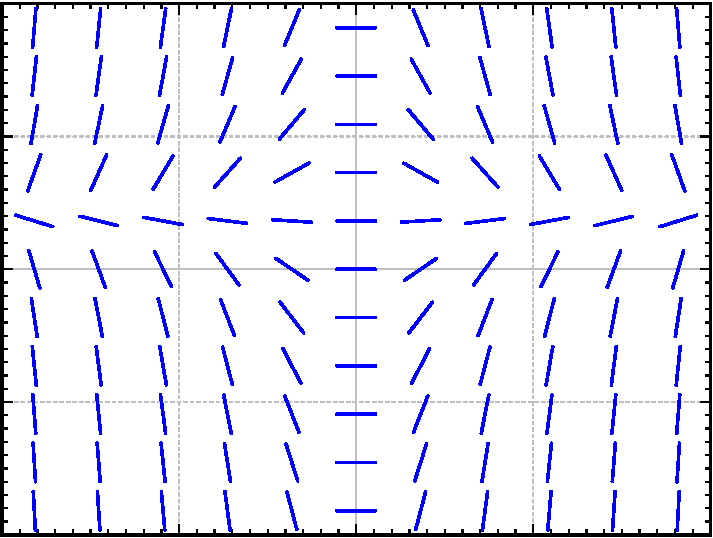
\includegraphics[width=1.75in]{figures/yprimex1minusyslope}}
		\task \parbox[c]{1.75in}{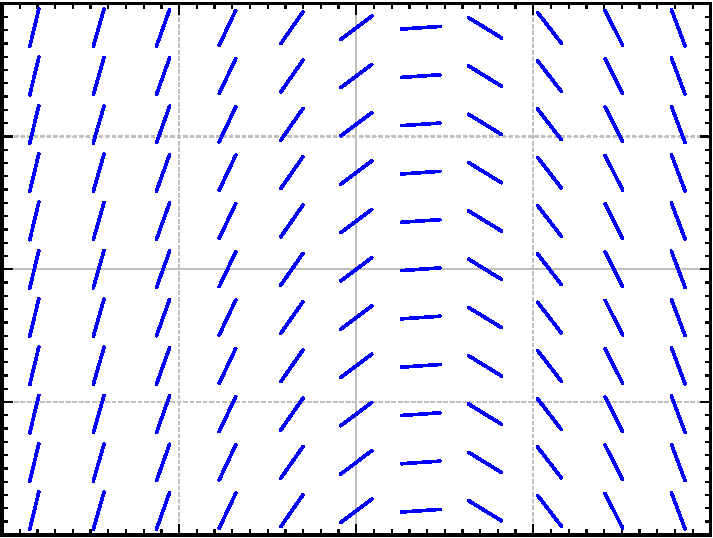
\includegraphics[width=1.75in]{figures/yprime1minusxslope}}
		\task \parbox[c]{1.75in}{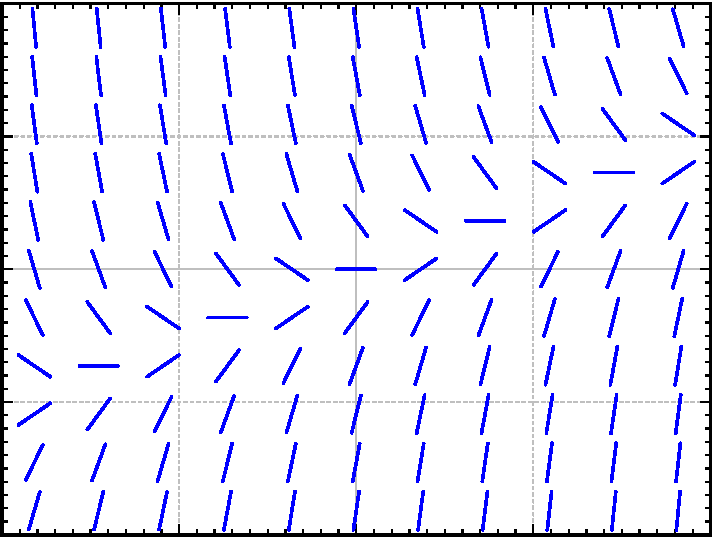
\includegraphics[width=1.75in]{figures/yprimexminus2yslope}}
	\end{tasks}
\end{exercise}
\end{samepage}

\begin{exercise}[défi]
	Soit $y' = f(x,y)$, $y(0) = 0$, tel que $f(x,y) > 1$ pour tous $x$ et $y$.
	Si la solution existe  pour tout $x$,  que peut-on dire à propos de $y(x)$ lorsque $x$ tend vers l'infini?  Expliquez.
\end{exercise}

\begin{exercise}[défi]
	Soit $(y-x)y' = 0$, $y(0) = 0$.
	\begin{tasks}
		\task Trouvez deux solutions distinctes.
		\task Expliquez pourquoi ceci ne contredit pas le théorème de Picard.
	\end{tasks}
\end{exercise}

\begin{exercise}
	Soit $y' = f(x,y)$.  Dites ce que vous savez à propos de son champ de directions,
	et dessinez un exemple, si vous avez l'information suivante à propos de  $f(x,y)$:
	\begin{tasks}(2)
		\task $f$ ne dépend pas de $y$.
		\task $f$ ne dépend pas de $x$.
		\task $f(t,t) = 0$ pour toute valeur $t$.
		\task $f(x,0) = 0$ et $f(x,1) = 1$ pour tout $x$.
	\end{tasks}
\end{exercise}

\begin{exercise}
	Trouvez une solution à $y' = \lvert y \rvert$, $y(0) = 0$.  Peut-on appliquer le théorème de Picard?
\end{exercise}

\begin{exercise}
	Soit $y' = (y-2x) g(x,y) + 2$, où $g(x,y)$ est une fonction quelconque.
	Pouvez-vous résoudre l'équation avec condition initiale $y(0) = 0$, et si oui, quelle est la solution?
\end{exercise}

\begin{exercise}[défi]
	\pagebreak[2]
	Soit $y' = f(x,y)$ tel que $f(x,1) = 0$ pour tout $x$,
	$f$ est continue et $\frac{\partial f}{\partial y}$ existe et est continue pour tous $x$ et $y$.
	\begin{tasks}
		\task Devinez une solution pour la condition initiale $y(0) = 1$.
		\task Les graphes de deux solutions ayant des conditions initiales différentes peuvent-elles s'intersecter?
		\task En supposant que $y(0) = 0$, que peut-on dire à propos de la solution?
				En particulier, peut-on avoir $y(x) > 1$ pour un certain $x$?
				Peut-on avoir $y(x) = 1$ pour un certain  $x$?  Pourquoi ou pourquoi pas?
	\end{tasks}
\end{exercise}

\setcounter{exercise}{100}

\begin{exercise}
	Dessiner le champ de directions pour $y'=y^3$.  Pouvez-vous identifier visuellement une solution telle que $y(0)=0$?
\end{exercise}
\exsol{%
	\\[6pt]
	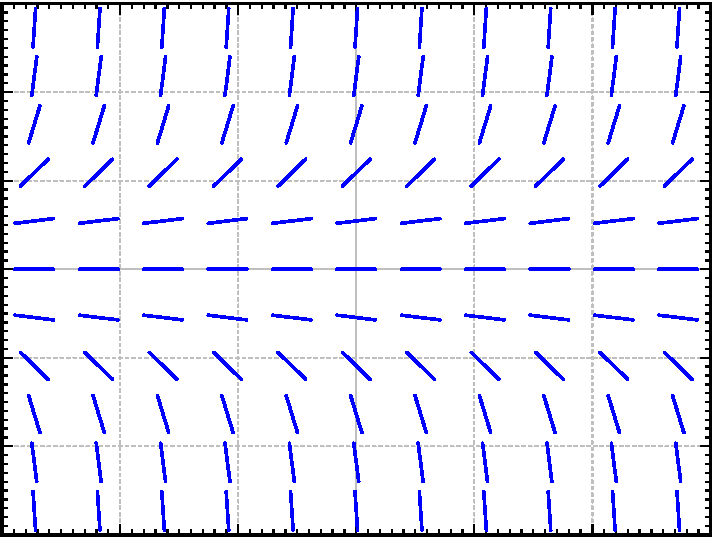
\includegraphics[width=2in]{figures/yprimey3slope}
	\\
	$y=0$ est une solution telle que $y(0)=0$.
}

\begin{exercise}
	Est-il possible de résoudre $y' = xy$, $y(0) = 0$?  La solution est-elle unique?
\end{exercise}
\exsol{%
	Oui une solution existe.  Car $y' = f(x,y)$ où $f(x,y) = xy$.  La fonction
	$f(x,y)$ est continue et
	$\frac{\partial f}{\partial y} = x$, qui est aussi continue près de $(0,0)$.
	Par conséquent, la solution existe et est unique.  (En fait $y=0$ est une solution).
}

\begin{exercise}
	Peut-on résoudre $y' = \frac{x}{x^2-1}$, $y(1) = 0$?
\end{exercise}
\exsol{%
	Non puisque la seule solution possible n'est pas définie au point $(x,y) = (1,0)$.
}

\begin{samepage}
\begin{exercise}
	Associez les équations suivantes, $y'=\sin x$, $y'=\cos y$, $y' = y\cos(x)$ à leurs champs de directions respectifs.
	Justifiez votre réponse.
	\begin{tasks}(3)
		\task	\parbox[c]{1.75in}{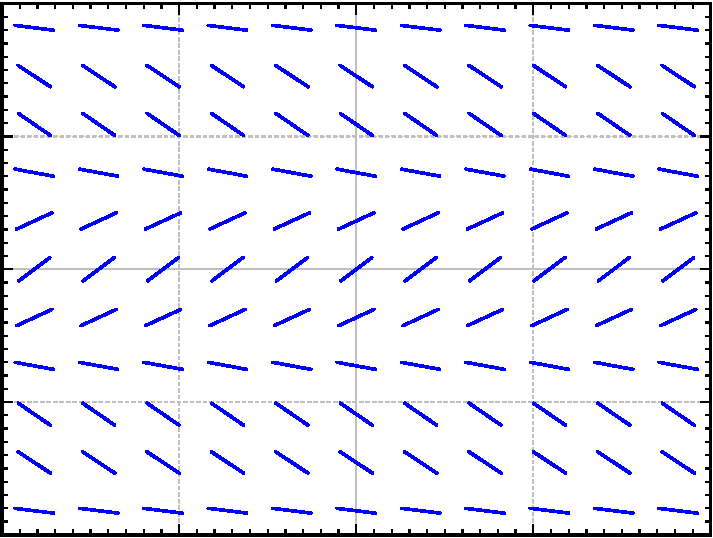
\includegraphics[width=1.75in]{figures/yprimecosyslope}}
		\task	\parbox[c]{1.75in}{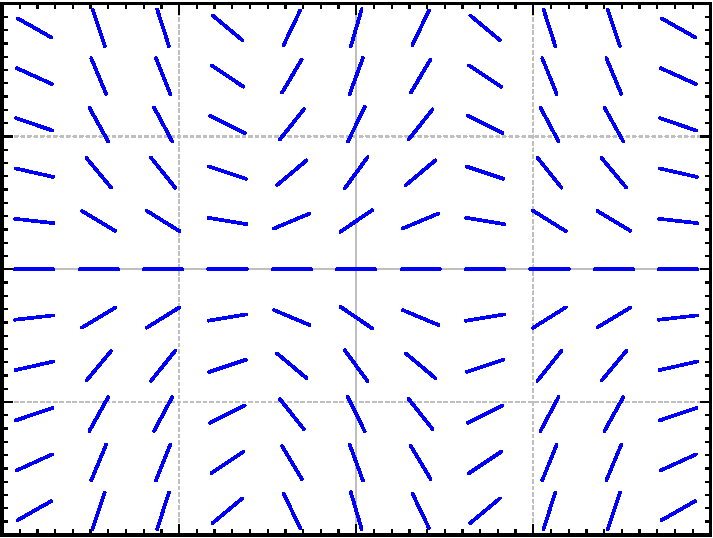
\includegraphics[width=1.75in]{figures/yprimecosxyslope}}
		\task	\parbox[c]{1.75in}{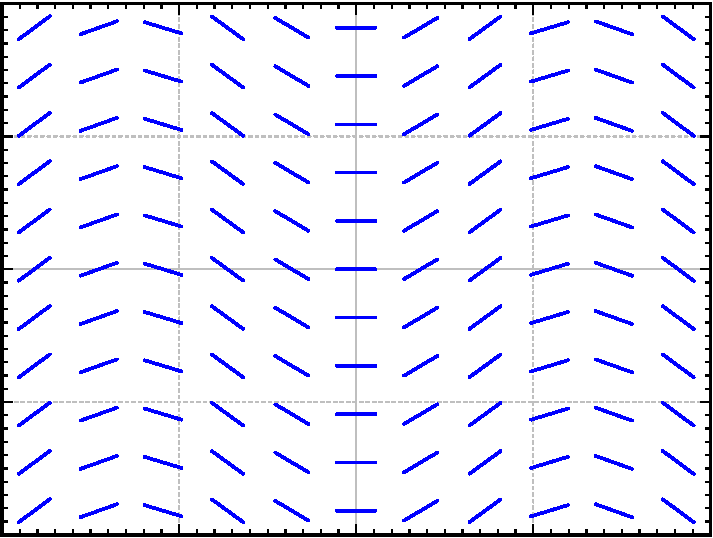
\includegraphics[width=1.75in]{figures/yprimesinxslope}}
	\end{tasks}
\end{exercise}
\end{samepage}
\exsol{%
	a) $y'=\cos y$, \quad
	b) $y' = y\cos(x)$, \quad
	c) $y'=\sin x$. \quad
	%Justification left to reader.
}

\begin{exercise}[défi]
	%[tricky]
	Supposons que
	\begin{equation*}
		f(y) = \begin{cases}
				0 & \text{ si $y > 0$}, \\
				1 & \text{ si $y \leq 0$} .
				\end{cases}
	\end{equation*}
	Est-ce que $y' = f(y)$, $y(0) = 0$ admet une solution dont la dérivée est continue?
	Le théorème de Picard s'applique-t-il?  Pourquoi ou pourquoi pas?
\end{exercise}
\exsol{%
	Picard ne s'applique pas puisque $f$ n'est pas continue en $y=0$.
	De plus, l'équation n'admet pas de solution dont la dérivée est continue.  Car si c'était vrai, alors il s'ensuivrait que
	$y'(0) = 1$.  Par le test de la première dérivée, $y(x) > 0$ pour de petites valeurs positives de $x$.
	Mais on a que $y'(x) = 0$ pour ces valeurs de $x$, et donc $y'$ n'est pas continue.
}

\begin{exercise}
	Considérons une équation de la forme $y' = f(x)$, où $f$ est une fonction continue quelconque,
	avec condition initiale $y(x_0) = y_0$.  Existe-t-il une solution pour tout $x$?  Pourquoi ou pourquoi pas?
\end{exercise}
\exsol{%
	La solution est $y(x) = \int_{x_0}^x f(s) \,ds + y_0$, ce qui existe pour toute valeur de $x$.
}

%%%%%%%%%%%%%%%%%%%%%%%%%%%%%%%%%%%%%%%%%%%%%%%%%%%%%%%%%%%%%%%%%%%%%%%%%%%%%%

\sectionnewpage
\section{Équations séparables}
\label{separable:section}

%\sectionnotes{1 lecture\EPref{, \S1.4 in \cite{EP}}\BDref{,
%\S2.2 in \cite{BD}}}

Lorsqu'une équation différentielle s'écrit sous la forme
$y' = f(x)$,
il suffit d'intégrer pour en obtenir la solution:
$y = \int f(x) \,dx + C$.
Malheureusement, cette technique ne fonctionne pas dans le cas général, c'est-à-dire
$y' = f(x , y)$, 
car si l'on intègre des deux côtés, on obtient:
\begin{equation*}
	y = \int f(x,y) \,dx + C .
\end{equation*}
Mais l'intégrale contient des termes en $y$, qu'on ne peut pas tout simplement \og{}traiter comme une constante\fg{}, puisque c'est une variable dépendante de $x$.


\subsection{Équations séparables}

On dit qu'une équation différentielle est \emph{\myindex{séparable}}
si elle peut être écrite sous la forme suivante:
\begin{equation*}
	y' = f(x)g(y),
\end{equation*}
où $f(x)$, $g(y)$ peuvent être des fonctions quelconques.
Écrivons cette équation à l'aide de la \myindex{notation de Leibniz}:
\begin{equation*}
	\frac{dy}{dx} = f(x)g(y) .
\end{equation*}
On peut alors réécrire l'équation comme suit:
\begin{equation*}
	\frac{dy}{g(y)} = f(x) \,dx .
\end{equation*}
Les deux côtés de l'équation sont des expressions qu'on peut intégrer:
\begin{equation*}
	\int \frac{dy}{g(y)} = \int f(x) \,dx + C .
\end{equation*}
Si l'on réussit à trouver des primitives de chaque côté, on pourra alors possiblement résoudre pour $y$.

\begin{example} \label{example:yprimeisxy}
	Prenons l'équation  suivante:
	\begin{equation*}
		y' = xy .
	\end{equation*}
	On observe que $y=0$ est une solution.  Nous gardons cette solution en mémoire et supposons maintenant que
	$y \not =0$, ce qui nous permettra de diviser par $y$.
	Écrivons l'équation comme suit: $\frac{dy}{dx} = xy$.  On intègre de chaque côté:
	\begin{equation*}
		\int \frac{dy}{y} = \int x\,dx + C .
	\end{equation*}
	On calcule les primitives de chaque côté et l'on obtient:
	\begin{equation*}
		\ln \, \lvert y\rvert = \frac{x^2}{2} + C
	\end{equation*}
	ou
	\begin{equation*}
		\lvert y \rvert = e^{\frac{x^2}{2} + C} = e^{\frac{x^2}{2}} e^C = D e^{\frac{x^2}{2}} ,
	\end{equation*}
	où $D > 0$ est une constante.  Puisque $y=0$ est aussi une solution et que, de plus, on a la valeur absolue de $y$, dans l'expression, on peut écrire:
	%
	\begin{equation*}
		y = D e^{\frac{x^2}{2}} ,
	\end{equation*}
	où $D$ est une constante quelconque, pouvant être 0 ou négative.  Vérifions que c'est une solution:
	\begin{equation*}
		y' = D x e^{\frac{x^2}{2}} = x \left( D e^{\frac{x^2}{2}} \right) = xy .
	\end{equation*}
\end{example}

Regardons de plus près cette méthode.  On pourrait s'inquiéter du fait que les deux intégrales apparaissant dans l'expression soient en termes de variables différentes.  Ça peut sembler erroné... Alors, nous allons revoir la méthode de séparation des variables de manière plus rigoureuse.

Supposons donc qu'on a:
\begin{equation*}
	\frac{dy}{dx} = f(x)g(y) .
\end{equation*}
Observons que $y = y(x)$ est une fonction de $x$ et que
$\frac{dy}{dx}$ l'est également.  On peut donc réécrire l'équation comme suit:
\begin{equation*}
	\frac{1}{g(y)}\,\frac{dy}{dx} = f(x) .
\end{equation*}
Maintenant, intégrons les deux côtés par rapport à $x$:
\begin{equation*}
	\int \frac{1}{g(y)}\,\frac{dy}{dx} \,dx = \int f(x) \,dx + C .
\end{equation*}
On fait un changement de variables dans l'intégrale de gauche:
\begin{equation*}
	\int \frac{1}{g(y)}\,dy = \int f(x) \,dx + C .
\end{equation*}
Comme on peut voir, on obtient la même formule que plus haut, qui est donc correcte.




\subsection{Solutions implicites}

Parfois, on peut avoir de la difficulté avec la méthode des équations séparables,
même si les deux intégrales sont résolubles.
Considérons, par exemple, l'équation séparable suivante:
\begin{equation*}
	y' = \frac{xy}{y^2+1} .
\end{equation*}
On sépare les variables:
\begin{equation*}
	\frac{y^2+1}{y}\,dy = \left(y+\frac{1}{y}\right)\,dy = x\,dx .
\end{equation*}
On intègre:
\begin{equation*}
	\frac{y^2}{2} + \ln \, \lvert y \rvert = \frac{x^2}{2} + C.
\end{equation*}
Puis, on réécrit pour rendre la solution plus jolie (ici, $D = 2C$):
\begin{equation*}
	y^2 + 2 \ln \, \lvert y\rvert = x^2 + D .
\end{equation*}
Il est difficile de trouver une expression explicite pour $y$, puisqu'on ne peut pas l'isoler dans l'expression.
Dans un tel cas, on obtient ce qu'on appelle une
\emph{\myindex{solution implicite}}.
On peut tout de même vérifier qu'on a bien trouvé une solution à l'équation différentielle.
Il suffit de dériver chaque côté par rapport à $x$, en se souvenant que $y$ est une fonction de $x$, et l'on obtient:
\begin{equation*}
	y'\left(2y + \frac{2}{y}\right) = 2x .
\end{equation*}
En multipliant les deux côtés par $y$ et en divisant par $2(y^2+1)$, on retrouve l'équation différentielle de départ (vérifiez-le).

Étant donné une solution implicite, trouver des valeurs de $y$ explicitement peut être difficile.
Il est possible qu'une valeur de $x$ donne plusieurs valeurs possibles de $y$ et qu'il faille alors choisir.
Parfois, il est plus simple de penser à $x$ comme à une fonction de $y$.  Parfois, même ceci est difficile.

Dans ce cas, un ordinateur peut être votre ami.  La plupart des logiciels mathématiques proposent
une fonction pour tracer la courbe-solution d'une équation implicite.
Par exemple, pour $C=0$, l'ensemble des points $(x,y)$ satisfaisant à  $y^2+2\ln|y|=x^2$
est une union de deux courbes, illustrées à la \figureref{implicitsols:fig}.
Ce n'est pas le graphe d'une fonction, puisque chaque $x$ admet deux valeurs possibles de $y$.
Mais si l'on choisit une des deux courbes, on a alors le graphe d'une fonction.
Si, de plus, on a une condition initiale, on choisit la courbe qui passe par ce point.
Ainsi, chaque valeur de $C$ donne deux solutions.
Comme on peut voir, les solutions implicites ne sont pas simples, mais parfois on ne peut pas obtenir mieux.

\begin{myfig}
	\capstart \diffyincludegraphics{width=3in}{width=4.5in}{implicitsols}
	\caption{Solution implicite $y^2+2\ln|y|=x^2$ à l'équation $y'=\frac{xy}{y^2+1}$.\label{implicitsols:fig}}
\end{myfig}

Cet exemple admet aussi la solution $y=0$.
Ainsi, la solution générale est
\begin{equation*}
	y^2 + 2 \ln \, \lvert y \rvert = x^2 + C \qquad \text{ou} \qquad y=0.
\end{equation*}
Des solutions comme $y=0$
sont parfois appelées des \emph{solutions singulières\index{solutions singulières}}.



\subsection{Exemples d'équations séparables}

\begin{example}
	Résolvons $x^2y' = 1 - x^2+y^2 - x^2y^2$, $y(1) = 0$.

	On factorise le côté droit:
	\begin{equation*}
		x^2y' = (1 - x^2)(1+y^2) .
	\end{equation*}
	On sépare les variables, on intègre et l'on résout pour $y$:
	\begin{align*}
		\frac{y'}{1+y^2} & = \frac{1 - x^2}{x^2} , \\
		\frac{y'}{1+y^2} & = \frac{1}{x^2} - 1 , \\
		\operatorname{arctan} (y) & = \frac{-1}{x} - x + C , \\
		y & = \tan \left(\frac{-1}{x} - x + C\right) .
	\end{align*}
	Il reste à résoudre pour la condition initiale,
	 $0 = \tan(-2+C)$, et l'on obtient $C=2$ (ou $C = 2 +
	\pi$, ou $C = 2 + 2\pi$, etc.).  La solution particulière recherchée est donc
	\begin{equation*}
		y = \tan \left(\frac{-1}{x} - x + 2 \right) .
	\end{equation*}
\end{example}

\begin{example} \label{sep:coffeeexample}
	Alex se prépare une tasse de café, qui doit se rendre à 60 degrés (Celsius) parce qu'Alex n'aime pas se brûler.
	Initialement, à $t=0$ minute,
	le café était à 89 degrés.  Une minute plus tard, Alex mesure la température de nouveau, et c'est 85 degrés.
	La température ambiante est 22 degrés.  Quand est-ce qu'Alex pourra enfin déguster son café?

	Posons $T$, la température du café en degrés Celsius, et $A$, la température ambiante, toujours en degrés Celsius.
	La 	\myindex{loi de refroidissement de Newton} affirme que le taux de changement de la température du café est
	proportionnel à la différence entre la température du café et la température ambiante.  Autrement dit:
	%
	\begin{equation*}
		\frac{dT}{dt} = k(A-T),
	\end{equation*}
	où $k$ est une constante.
	Dans notre exemple: $A=22$, $T(0) = 89$, $T(1) = 85$.
	On sépare les variables et l'on intègre (ici, $C$ et $D$ sont des constantes arbitraires):
	\begin{align*}
		\frac{1}{T-A} \, \frac{dT}{dt} & = -k , \\
							\ln (T-A)  &= -kt + C , \qquad \text{(notons que } T-A > 0 \text{)} \\
								T-A    &= D\, e^{-kt} ,  \\
								T      &= A + D\, e^{-kt} .
	\end{align*}
	En substituant la valeur de $A$, on a
	$T = 22 + D\, e^{-kt}$.
	On substitue la condition initiale: $89 = T(0) = 22 + D$,
	et donc $D = 67$.
	Ainsi,  $T = 22 + 67\, e^{-kt}$.
	La deuxième condition donne que $85 = T(1) = 22 + 67\, e^{-k}$.
	En résolvant pour $k$, on obtient 	$k = - \ln \frac{85-22}{67} \approx 0{,}0616$.
	Maintenant, trouvons la valeur de $t$ donnant une température de 60 degrés.
	On résout l'équation suivante,
	\begin{equation*}
		60 = 22 + 67 e^{-0{,}0616t}
	\end{equation*}
	pour obtenir
	$t = - \frac{\ln \frac{60-22}{67}}{0{,}0616} \approx 9{,}21$ minutes.
	Donc, Alex peut commencer à boire son café environ 9 minutes après l'avoir préparé (correspondant à peu près au temps requis pour faire ce calcul).  Voir la \figureref{sintro:coffeefig}.
	\begin{myfig}
		%original files coffeefig-1 coffeefig-2
		\capstart		\diffyincludegraphics{width=6.24in}{width=9in}{coffeefig-1-2}
		\caption{Graphes de la fonction de température du café $T(t)$.
		À gauche, des droites horizontales sont tracées aux températures 60, 85 et 89.
		Des droites verticales sont tracées à $t=1$ et à $t=9{,}21$.
		Observez que la température atteint la valeur 85 à $t=1$, et 60 à
		$t \approx 9{,}21$.  À droite, le graphe montre la température pour une plus longue durée,
		avec une droite horizontale à la valeur de la température ambiante, soit 22.\label{sintro:coffeefig}}
	\end{myfig}
\end{example}

\begin{example}
	Trouvons la solution générale de $y' = \frac{-xy^2}{3}$ (incluant les solutions singulières).

	Notons d'abord que $y=0$ est une solution (singulière).
	Supposons donc pour la suite que $y \not= 0$.  On sépare les variables et l'on intègre:
	\begin{align*}
		\frac{-3}{y^2} y' & = x  \displaybreak[0]\\
			\frac{3}{y}   & = \frac{x^2}{2} + C  \displaybreak[0]\\
						y & = \frac{3}{\nicefrac{x^2}{2} + C} = \frac{6}{x^2 + 2C}.
	\end{align*}
	La solution générale est donc
	\begin{align*}
		y = \frac{6}{x^2 + 2C} \qquad \text{ou} \qquad y=0 .
	\end{align*}
\end{example}

\subsection{Exercices}

\begin{exercise}
	Résolvez $y' = \nicefrac{x}{y}$.
\end{exercise}

\begin{exercise}
	Résolvez$y' = x^2y$.
\end{exercise}

\begin{exercise}
	Résolvez $\dfrac{dx}{dt} = (x^2-1)\,t$, $x(0) = 0$.
\end{exercise}

\begin{exercise}
	Résolvez $\dfrac{dx}{dt} = x\,\sin(t)$, for $x(0) = 1$.
\end{exercise}

\begin{exercise}
	Résolvez $\dfrac{dy}{dx} = xy+x+y+1$.  Indice: factorisez le côté droit.
\end{exercise}

\begin{exercise}
	Résolvez $xy' = y + 2x^2 y$, $y(1) = 1$.
\end{exercise}

\begin{exercise}
	Résolvez$\dfrac{dy}{dx} = \dfrac{y^2+1}{x^2+1}$, $y(0) = 1$.
\end{exercise}

\begin{exercise}
	Trouvez une solution implicite pour
	$\dfrac{dy}{dx} = \dfrac{x^2+1}{y^2+1}$, $y(0) = 1$.
\end{exercise}

\begin{exercise}
	Trouvez une solution explicite pour $y' = xe^{-y}$, $y(0)=1$.
\end{exercise}

\begin{exercise}
	Trouvez une solution explicite pour $xy' = e^{-y}$, $y(1)=1$.
\end{exercise}

\begin{exercise}
	Trouvez une solution explicite pour $y' = ye^{-x^2}$, $y(0)=1$.
	Au besoin, votre réponse peut inclure une intégrale.
\end{exercise}

\begin{exercise}
	Supposons qu'une tasse de café est à 100 degrés Celsius au temps $t=0$,
	et 70 degrés à $t=10$ minutes, et 50 degrés à $t=20$ minutes.
	Calculez la température ambiante.
\end{exercise}

\setcounter{exercise}{100}

\begin{exercise}
Résolvez $y'=2xy$.
\end{exercise}
\exsol{%
	$y = Ce^{x^2}$
}

\begin{exercise}
	Résolvez $x'=3xt^2-3t^2$, $x(0)=2$.
\end{exercise}
\exsol{%
	$x = e^{t^3}+1$
}

\begin{exercise}
	Trouvez une solution implicite pour $x'=\frac{1}{3x^2+1}$, $x(0)=1$.
\end{exercise}
\exsol{%
	$x^3+x=t+2$
}

\begin{exercise}
	Trouvez une solution explicite pour $x y' = y^2$, $y(1) = 1$.
\end{exercise}
\exsol{%
$y = \frac{1}{1-\ln x}$
}

\begin{exercise}
Trouvez une solution implicite pour $y' = \frac{\sin(x)}{\cos(y)}$.
\end{exercise}
\exsol{%
$\sin(y) = -\cos(x) + C$
}

\begin{exercise}
	Reprenez l'\exampleref{sep:coffeeexample} avec les mêmes valeurs: 89 degrés à $t=0$, 85 degrés à $t=1$, et une température ambiante de 22 degrés.
	Supposons que ces températures ont été mesurées avec une précision de $\pm 0.5$ degrés.
	À cause de cette imprécision, on ne connaît qu'un intervalle de temps pour
	que la température du café atteigne exactement 60 degrés.
	Trouvez cet intervalle de temps.
	Indice: quel type d'erreur rend le temps de refroidissement plus long? Plus court?
\end{exercise}
\exsol{%
	L'intervalle de temps est d'environ 7.45 à 12.15 minutes.
}

\begin{exercise}
	Une population de lapins $x$ sur une île est modelisée par l'équation suivante:
	$x' = x- \bigl(\nicefrac{1}{1000} \bigr) x^2$,
	où la variable indépendante $t$ est le temps, mesuré en mois.
	À  $t=0$, l'île contient 40 lapins.
	\begin{tasks}
		\task Résolvez l'équation différentielle avec condition initiale.
		\task Combien de lapins habitent l'île après 1 mois, 5 mois, 10 mois, 15 mois?  Arrondissez à l'entier le plus proche.
	\end{tasks}
\end{exercise}
\exsol{%
	a) $x = \frac{1000e^t}{e^t+24}$. \quad b) 102 lapins après un mois,
	861 après 5 mois, 999 après 10 mois, 1000 après 15 mois.
}

%%%%%%%%%%%%%%%%%%%%%%%%%%%%%%%%%%%%%%%%%%%%%%%%%%%%%%%%%%%%%%%%%%%%%%%%%%%%%%

\sectionnewpage
\section{Équations linéaires et facteur intégrant}
\label{intfactor:section}

%\sectionnotes{1 lecture\EPref{, \S1.5 in \cite{EP}}\BDref{,
%\S2.1 in \cite{BD}}}

Les \emph{équations linéaires\index{équation linéaire}} sont parmi les équations différentielles les plus importantes à comprendre.
Une bonne partie des équations que nous voyons dans ce manuel sont en fait linéaires.
Cette section est dédiée aux \emph{\myindex{équations linéaires du premier ordre}}.
Une équation du premier ordre est dite linéaire si elle peut s'écrire sous la forme suivante :
\begin{equation} \label{lineq:eq1}
y' + p(x) y = f(x) .
\end{equation}
Être \og{}linéaire\fg{} veut dire que l'expression est linéaire en $y$ et $y'$;
l'équation ne contient pas de puissances plus élevées ni d'autres fonctions de $y$ ou $y'$.
Cependant, la dépendance sur la variable $x$ peut être plus compliquée.

La raison pour laquelle on aime les équations linéaires, c'est qu'elles ont de belles propriétés.
Par exemple, la solution existe pour tout $x$ où $p(x)$ et $f(x)$ sont définies (voir de plus la remarque~\ref{rem:regular}).
Ce qui nous intéressera surtout, à ce stade-ci, c'est qu'il y a une méthode générale pour résoudre les équations linéaires du premier ordre.

L'idée: réécrire le côté gauche de  \eqref{lineq:eq1} comme une dérivée du produit de $y$ avec une fonction à déterminer.
Ainsi, nous cherchons une fonction $r(x)$ telle que :
\begin{equation*}
	r(x) y' + r(x) p(x) y = \frac{d}{dx}\Bigl[ r(x) y \Bigr].
\end{equation*}
Ceci est le côté gauche de \eqref{lineq:eq1} multiplié par $r(x)$.
Donc, si l'on multiplie \eqref{lineq:eq1} par $r(x)$, on obtient:
\begin{equation*}
	\frac{d}{dx}\Bigl[ r(x) y \Bigr] = r(x)f(x) .
\end{equation*}
Maintenant, on intègre les deux côtés.
C'est possible puisque le côté droit ne dépend pas de $y$ et que le côté gauche est la dérivée d'une fonction.
Ensuite, on résout pour  $y$.
La fonction $r(x)$ s'appelle le \emph{\myindex{facteur intégrant}} et la méthode s'appelle la
\emph{\myindex{méthode du facteur intégrant}}.

Comment trouver $r(x)$?  On cherche une fonction qui, lorsqu'on la dérive, donne  de nouveau la fonction, multipliée par $p(x)$.
Les fonctions exponentielles ont précisément cette propriété.  On pose donc:
%
\begin{equation*}
r(x) = e^{\int p(x) \,dx} .
\end{equation*}
On substitue cette valeur dans l'équation différentielle pour obtenir ce qui suit:
\begin{align*}
											y' + p(x) y  &= f(x) , \\
	e^{\int p(x) \,dx} y' + e^{\int p(x) \,dx} p(x) y    & = e^{\int p(x) \,dx} f(x) , \\
	\frac{d}{dx}\left[ e^{\int p(x) \,dx} y \right]      & = e^{\int p(x) \,dx} f(x) , \\
									e^{\int p(x) \,dx} y & = \int e^{\int p(x) \,dx} f(x) \,dx + C , \\
													y    & = e^{-\int p(x) \,dx} \left( \int e^{\int p(x) \,dx} f(x) \,dx + C \right) .
\end{align*}

On pourra obtenir une formule analytique pour $y$,
à condition de pouvoir trouver les primitives de chacune des intégrales apparaissant dans l'expression.

\begin{example}
	Résolvons
	\begin{equation*}
		y' + 2xy = e^{x-x^2}, \qquad y(0) = -1 .
	\end{equation*}

	Notons d'abord que $p(x) = 2x$ et que $f(x) = e^{x-x^2}$.
	Le facteur intégrant est $r(x) = e^{\int p(x)\, dx} = e^{x^2}$.
	On multiplie chaque côté de l'équation par $r(x)$ pour obtenir:
	\begin{align*}
		e^{x^2} y' + 2xe^{x^2}y & = e^{x-x^2} e^{x^2} , \\
		\frac{d}{dx} \left[ e^{x^2} y \right] &= e^x .
	\end{align*}
	On intègre:
	\begin{align*}
		e^{x^2} y &= e^x +C , \\
		y &= e^{x-x^2} + C e^{-x^2} .
	\end{align*}
	Ensuite, on résout pour la condition initiale $-1 = y(0) = 1 + C$, ce qui donne $C=-2$.
	La solution est donc:
	\begin{equation*}
		y = e^{x-x^2} - 2 e^{-x^2} .
	\end{equation*}
\end{example}
Notons que nous pouvons prendre la primitive de notre choix pour
$e^{\int p(x) dx}$.  On peut ajouter une constante d'intégration, mais ça ne changera pas la réponse à la fin.

\begin{exercise}
	Essayez-le\textit{:} ajoutez une constante d'intégration au facteur intégrant dans l'exemple et vérifiez que vous obtenez la même solution qu'ici.
\end{exercise}

Conseil: plutôt que d'apprendre par c{\oe}ur la formule, retenez plutôt la méthode pour l'obtenir.
C'est plus simple, et il suffit alors de répéter la méthode pour résoudre le problème.

Puisqu'on ne peut pas toujours trouver une solution analytique, il peut être utile de savoir comment écrire la solution sous forme d'intégrale définie, car une intégrale définie peut être traitée par un logiciel de calcul.  Soit l'équation suivante:
\begin{equation*}
	y' + p(x) y = f(x) , \qquad y(x_0) = y_0 .
\end{equation*}
Écrivons la solution sous forme d'intégrale définie:
\begin{equation} \label{lei:defsol}
\mybxbg{
~~
y(x) = e^{-\int_{x_0}^x p(s)\, ds} \left( \int_{x_0}^x e^{\int_{x_0}^t p(s)\, ds}
f(t) \,dt + y_0 \right).
~~
}
\end{equation}
Cette formule peut maintenant être lue par une application de calcul numérique,  si nous la codons convenablement.

\begin{exercise}
	Vérifiez que $y(x_0) = y_0$ dans \eqref{lei:defsol}.
\end{exercise}

\begin{exercise}
	Écrivez la solution du problème suivant sous forme d'intégrale définie.  Vous ne pourrez pas trouver une solution analytique à cette équation.
	%
	\begin{equation*}
		y' + y = e^{x^2-x}, \qquad y(0) = 10 .
	\end{equation*}
\end{exercise}

\begin{remark}\label{rem:regular}
	Avant de continuer, notons quelques propriétés intéressantes des équations linéaires.  Premièrement, il existe toujours une formule explicite \eqref{lei:defsol} pour la
	solution de l'équation à condition initiale
	$y' + p(x) y = f(x)$, $y(x_0) = y_0$.  Deuxièmement, la formule
	\eqref{lei:defsol} implique que si $p(x)$
	et $f(x)$ sont continues sur un intervalle $(a , b)$, alors la solution
	$y(x)$ existe et est différentiable sur $(a , b)$.  Comparez à l'exemple non linéaire vu précédemment, $y'=y^2$,
	ainsi qu'au \thmref{slope:picardthm}.
\end{remark}


\begin{example}
	Voyons maintenant une application des équations linéaires qui est couramment rencontrée: la concentration de produits chimiques dans un plan d'eau.

	\begin{mywrapfigsimp}{1.60in}{1.65in}
	\noindent
	\inputpdft{lin-tank}
	\end{mywrapfigsimp}
	Un réservoir d'une capacité de 100 litres contient 10 kilogrammes de sel dissous dans 60 litres d'eau.  Une solution d'eau saline avec une concentration de 0,1 kilogrammes par litre entre dans le réservoir à un taux de 5 litres par minute. La solution dans le réservoir est bien brassée (c'est-à-dire qu'on peut supposer que la concentration est la même partout) et sort à un taux de 3 litres par minute.  Combien de sel est contenu dans le réservoir lorsqu'il est plein?

	Commençons par établir l'équation différentielle modélisant ce problème.  Dénotons par $x$ la quantité de sel dans le réservoir, en kilogrammes,  et par $t$ le temps en minutes.  Si l'on considère une petite variation $\Delta t$ dans le temps, la variation en $x$ (dénotée $\Delta x$) est approximativement :
	\begin{equation*}
		\Delta x \approx
		(\text{taux entrée} \times \text{concentration entrée}) \Delta t -
		(\text{taux sortie} \times \text{concentration sortie}) \Delta t .
	\end{equation*}
	On divise partout par $\Delta t$ et l'on prend la limite $\Delta t \to 0$ pour obtenir:
	\begin{equation*}
		\frac{dx}{dt} =
		(\text{taux entrée} \times \text{concentration entrée})  -
		(\text{taux sortie} \times \text{concentration sortie}) .
	\end{equation*}
	Dans notre exemple:
	\begin{align*}
		\text{taux entrée} &= 5 , \\
		\text{concentration entrée} &= 0,1 , \\
		\text{taux sortie} &= 3 , \\
		\text{concentration sortie} &= \frac{x}{\text{volume}} = \frac{x}{60+(5-3)t} .
	\end{align*}
	L'équation modélisant le problème est donc:
	\begin{equation*}
		\frac{dx}{dt} =	(5 \times 0,1)  - 	\left(3 \frac{x}{60+2t}\right) .
	\end{equation*}
	On réécrit ceci sous la forme \eqref{lineq:eq1}:
	\begin{equation*}
		\frac{dx}{dt} + 	\frac{3}{60+2t} x = 	0.5 .
	\end{equation*}

	Maintenant, on peut résoudre l'équation.  Le facteur intégrant est:
	\begin{equation*}
		r(t) = \exp \left( \int \frac{3}{60+2t} dt  \right)
		= 	\exp \left( \frac{3}{2} \ln (60+2t) \right)
		= 	{(60+2t)}^{3/2} .
	\end{equation*}

	On multiplie les deux côtés de l'équation par le facteur intégrant et l'on obtient:
	\begin{align*}
	{(60+2t)}^{3/2} \frac{dx}{dt} + {(60+2t)}^{3/2} \frac{3}{60+2t} x
		& = 	0,5{(60+2t)}^{3/2} \\
	\frac{d}{dt}\left[{(60+2t)}^{3/2} x \right]
		& = 0,5{(60+2t)}^{3/2} \\
	{(60+2t)}^{3/2} x
		& = \int  0,5{(60+2t)}^{3/2} dt +C \\
	 x	& = 	{(60+2t)}^{-3/2} \int  \frac{{(60+2t)}^{3/2}}{2}dt
					+C{(60+2t)}^{-3/2} \\
	 x	& =	{(60+2t)}^{-3/2}\frac{1}{10}{(60+2t)}^{5/2}	+C{(60+2t)}^{-3/2} \\
	 x	& = \frac{60+2t}{10}+C{(60+2t)}^{-3/2} .
	\end{align*}

	%mbxSTARTIGNORE
	\begin{mywrapfig}{3.25in}
		\capstart\diffyincludegraphics{width=3in}{width=4.5in}{linear-salt-graph}
		\caption{Graphe de la solution $x$ kilogrammes de sel dans le réservoir au temps $t$.\label{linear-salt-graph:fig}}
	\end{mywrapfig}
	%mbxENDIGNORE
	%
	% Make sure to keep the above and the mbx figure below in sync!
	%
	On doit trouver la valeur de $C$.  On sait qu'à $t=0$, $x=10$.
	Donc,
	\begin{equation*}
		10 = x(0) 	= 	\frac{60}{10}+C{(60)}^{-3/2} =6 +C{(60)}^{-3/2}
	\end{equation*}
	ou
	\begin{equation*}
		C=4 ({60}^{3/2}) \approx 1859{,}03 .
	\end{equation*}

	On cherche à savoir la valeur de $x$ lorsque le réservoir est plein.  Ceci arrive lorsque $60+2t = 100$, c'est-à-dire à  $t=20$.  Donc:
	\begin{equation*}
	\begin{split}
		x(20) & = 	\frac{60+40}{10}+C{(60+40)}^{-3/2}	\\
	 		& \approx	10 +1859,03 {(100)}^{-3/2} \approx 11,86 .
	\end{split}
	\end{equation*}
	Voir la \figureref{linear-salt-graph:fig} pour le graphe de $x$ en fonction de $t$.

	La concentration dans le réservoir plein est approximativement \unitfrac[0{,}1186]{kg}{litre},
	alors que la concentration initiale est de $\nicefrac{1}{6}$ ou \unitfrac[0{,}167]{kg}{litre}.
	%mbxlatex \begin{myfig}
	%mbxlatex \capstart
	%mbxlatex \diffyincludegraphics{width=3in}{width=4.5in}{linear-salt-graph}
	%mbxlatex \caption{Graph of the solution $x$ kilograms of salt in the tank at time
	%mbxlatex $t$.\label{linear-salt-graph:fig}}
	%mbxlatex \end{myfig}
\end{example}

\subsection{Exercices}

Dans les exercices suivants, n'hésitez pas à laisser la réponse sous forme d'intégrale définie
si une solution analytique n'est pas possible.
Mais si la solution analytique existe, c'est celle-là que vous devriez donner.

\begin{exercise}
	Résolvez $y' + xy = x$.
\end{exercise}

\begin{exercise}
	Résolvez $y' + 6y = e^x$.
\end{exercise}

\begin{exercise}
	Résolvez $y' + 3x^2y = \sin(x) \, e^{-x^3}$, $y(0) = 1$.
\end{exercise}

\begin{exercise}
	Résolvez $y' + \cos (x) y = \cos(x)$.
\end{exercise}

\begin{exercise}
	Résolvez $\frac{1}{x^2+1} \, y' + x y = 3$, $y(0) = 0$.
\end{exercise}

\begin{exercise}
	Supposons que deux lacs se trouvent sur le plan d'un ruisseau. De l'eau propre s'écoule dans le premier lac, ensuite l'eau s'écoule du premier lac au deuxième lac, et enfin l'eau se déverse en aval du ruisseau à partir du deuxième lac. Le débit à l'entrée et à la sortie de chaque lac est 500 litres par heure.  Le premier lac contient 100 000 litres d'eau et le deuxième lac en contient 200 000.  Un camion déverse \unit[500]{kg} d'une matière dangereuse.  On suppose que l'eau est bien brassée par le ruisseau.
	\begin{tasks}
		\task Trouvez la concentration de la matière dangereuse dans chacun des lacs, en fonction du temps.
		\task À quel moment est-ce que la
		concentration dans le premier lac tombe en-dessous de  \unit[0.001]{kg} par litre?
		\task À quel moment est-ce que la concentration dans le deuxième sera maximale?
	\end{tasks}
\end{exercise}

\begin{exercise}
	La \myindex{loi de refroidissement de Newton} affirme que $\frac{dx}{dt} = -k(x-A)$, où
	$x$ est la température, $t$ est le temps, $A$ est la température ambiante,
	et $k > 0$ est une constante.
	Supposons que $A = A_0 \cos (\omega t)$, où $A_0$ et $\omega$ sont des constantes.  Autrement dit, la température ambiante oscille en fonction du temps (par exemple, varie entre le jour et la nuit).
	\begin{tasks}
	\task Trouvez la solution générale.
	\task Est-ce que les conditions initiales ont un impact sur le comportement à long terme de la solution?  Pourquoi ou pourquoi pas?
	\end{tasks}
\end{exercise}

\begin{exercise}
	Un réservoir contient 5 grammes de sel dissous dans 20 litres d'eau.
	Une solution saline, dont la concentration est de 2 grammes par litre,
	s'y déverse à un taux de 3 litres par minute.
	Le contenu du réservoir est bien brassé et en ressort à un taux de 3 litres par minute. Quelle doit être la durée du procédé pour obtenir 20 grammes de sel dans le réservoir?
\end{exercise}

\begin{exercise}
	Un réservoir contient 10 litres d'eau propre.
	Une solution saline, de concentration inconnue mais constante, se déverse dans le réservoir à un taux de 1 litre par minute.
	Le contenu du réservoir est bien brassé et en ressort à un taux de 1 litre par minute.
	Au bout de 20 minutes, le réservoir contient 15 grammes de sel.  Quelle est la concentration de la solution saline entrante?
\end{exercise}

\setcounter{exercise}{100}

\begin{exercise}
	Résolvez $y'+3 x^2 y = x^2$.
\end{exercise}
\exsol{%
	$y = C e^{-x^3} + \nicefrac{1}{3}$
}

\begin{exercise}
	Résolvez $y'+ 2\sin(2x) y = 2\sin(2x)$, $y(\nicefrac{\pi}{2}) = 3$.
\end{exercise}
\exsol{%
	$y = 2 e^{\cos(2x)+1} + 1$
}

\begin{exercise}
	Un réservoir d'eau est vidé à un taux de \unitfrac[3]{L}{min}.
	Au départ, le réservoir contient \unit[10]{L} d'eau propre.
	De l'eau contenant une matière dangereuse se déverse dans le réservoir à un taux de \unitfrac[2]{L}{min},
	ave une concentration de \unitfrac[$20t$]{g}{L} au temps $t$.
	Au moment où le réservoir est à moitié vide, combien de grammes de matière dangereuse sont contenus dans le réservoir?
	(On suppose que c'est bien brassé.)
\end{exercise}
\exsol{%
	$250$ grammes
}

\begin{exercise}
	Supposons qu'on ait une population de bactéries à laquelle on ajoute graduellement une substance toxique,
	de telle sorte que le taux de croissance diminue.  Plus précisément, $\frac{dP}{dt} = (2-0{,}1\,t)P$.
	Si $P(0) = 1000$, trouvez la population pour $t=5$.
\end{exercise}
\exsol{%
	$P(5) = 1000 e^{2 \times 5 - 0{,}05 \times {5}^2} = 1000 e^{8{,}75} \approx 6{,}31 \times {10}^6$
}

\begin{exercise}
	De l'eau se déverse dans un réservoir cylindrique à un débit de $d$ mètres cube par seconde.
	Soit $A$ l'aire d'une section transversale du réservoir, en mètres.
	Supposons que l'eau sort du réservoir à un débit qui est proportionnel à la hauteur du niveau d'eau.
	Trouvez l'équation différentielle décrivant $h$, la hauteur du niveau d'eau, en introduisant les constantes dont vous avez besoin.
	Donnez aussi les unités pour vos constantes.
\end{exercise}
\exsol{%
$Ah' = d - kh$, où $k$ est une constante mesurée en $\unit{m^2}{s}$.
}


%%%%%%%%%%%%%%%%%%%%%%%%%%%%%%%%%%%%%%%%%%%%%%%%%%%%%%%%%%%%%%%%%%%%%%%%%%%%%%

\sectionnewpage
\section{Équations autonomes}
\label{auteq:section}

%\sectionnotes{1 lecture\EPref{, \S2.2 in \cite{EP}}\BDref{,
%\S2.5 in \cite{BD}}}

Considérons une équation différentielle comme suit:
\begin{equation*}
	\frac{dx}{dt} = f(x),
\end{equation*}
où la dérivée dépend uniquement de $x$, la variable dépendante, et non de $t$, la variable indépendante.
De telles équations sont dites \emph{autonomes\index{équation autonome}}.
On dit \og{}autonome\fg{} parce que, si l'on pense à la variable indépendante comme étant le temps, la valeur de la dérivée à un point est la même à tout moment.

Reprenons, par exemple, le problème du café qui tiédit (\exampleref{sep:coffeeexample}).
\myindex{La loi de refroidissement de Newton} est une équation autonome:
\begin{equation*}
	\frac{dx}{dt} = k (A-x)
\end{equation*}
où $x$ est la température, $t$ est le temps, $k$ est une constante positive,
et $A$ est la température ambiante.
 Voir la \figureref{2.2:coffeefig} pour un exemple avec $k=0{,}3$ et $A=5$.

On remarque que l'équation admet la solution constante $x=A$ (dans la figure, $x=5$).
On appelle ces solutions constantes des \emph{solutions d'équilibre}\index{solution d'équilibre}.
Les points sur l'axe des $x$ où $f(x) = 0$ sont des \emph{points critiques\index{point critique}}.
Par exemple, le point  $x=A$ est un point critique. Notons que chaque point critique correspond à une solution d'équilibre.

Le graphe nous indique que la solution $x=A$ est \og{}stable\fg{},
c'est-à-dire que de petits changements dans $x$ ne mènent pas à
des changements importants dans les solutions lorsque $t$ augmente.
Si l'on modifie légèrement la condition initiale, alors $x(t) \to A$ lorsque $t \to \infty$.
Le point critique est alors appelé \emph{stable}\index{point critique stable}.
Dans l'exemple du refroidissement, toutes les solutions tendent vers $A$ lorsque $t \to \infty$.
Mais ce n'est pas toujours le cas.  Lorsqu'un point critique n'est pas stable, on l'appelle alors
\emph{instable}\index{point critique instable}.

\begin{myfig}
	\parbox[t]{3.0in}{
	 \capstart  \diffyincludegraphics{width=2.93in}{width=4.5in}{2-2-coffee}
	 \caption{Le champ de directions de
	 $x' = 0.3\,(5-x)$ et quelques solutions.\label{2.2:coffeefig}}
	 %$dx/dt = -0.3*(x-5)$, $t: [0,20], x: [-10,10]$, plot solutions for
	 %$t=0$, $x=10$, $x=5$, $x=0$, $x=-5$, $x=-10$.
	}
	\quad
	\parbox[t]{3.0in}{
	 \capstart  \diffyincludegraphics{width=3in}{width=4.5in}{2-2-logistic}
	 \caption{Le champ de directions de
	 $x' = 0.1\,x\,(5-x)$ et quelques solutions.\label{2.2:logisticfig}}
	}
\end{myfig}

\medskip

Considérons maintenant \emph{\myindex{l'équation logistique}}:
\begin{equation*}
	\frac{dx}{dt} = kx(M-x),
\end{equation*}
où $k$ et $M$ sont des constantes positives.
Cette équation sert communément à modéliser une population si l'on connaît la population limite $M$,
c'est-à-dire la capacité maximale du système.
Les prédictions issues d'une équation logistique sont moins catastrophiques que pour $x'=kx$.
Bien que $x$ ne puisse pas être négatif, en pratique, puisqu'il s'agit d'une population, la solution mathématique admet des valeurs négatives.

La \figureref{2.2:logisticfig} illustre l'exemple $x' = 0.1 x(5-x)$.
Il y a deux points critiques, $x=0$ et $x=5$.  Celui à
 $x=5$ est stable, alors que celui à $x=0$ est
instable.

On peut analyser le comportement à long terme des solutions sans devoir les déterminer exactement.
Le champ de directions de $x' = 0.1 x(5-x)$ nous montre que:
\begin{equation*}
	\lim_{t\to \infty} x(t) = 	\begin{cases}
								5 & \text{si } \; x(0) > 0 , \\
								0 & \text{si } \; x(0) = 0 , \\
								\text{n'existe pas ou } {-\infty} & \text{si } \; x(0) < 0 . \\
								\end{cases}
\end{equation*}
Quant au cas où $x(0) < 0$, il ne suffit pas de simplement observer le champ de directions.
Il se pourrait que la solution n'existe pas pour tout $t$ positif.
Rappelons l'exemple de $x' = x^2$ où les solutions existent seulement sur un intervalle fini.
Un tel scénario est possible ici.  Dans les faits, on trouverait ici que la solution n'existe
pas pour toutes les valeurs réelles -- et tend vers $-\infinity$ dans un temps fini --  mais, pour le voir, il faudrait résoudre l'équation.

Si l'on s'intéresse seulement au comportement à long terme de la solution, on n'a pas besoin de résoudre l'équation logistique exactement.
Il suffirait de dessiner le champ de directions.
En fait, on peut simplifier le travail encore plus,
en traçant ce qu'on appelle le \emph{\myindex{diagramme de phase}} ou
\emph{\myindex{portrait de phase}} de l'équation autonome.
Voici comment on fait dans un cas comme celui-ci, où il y a une seule variable dépendante $x$.
\begin{itemize}
	\item Nous traçons l'axe des $x$, nous y marquons tous les points critiques de l'équation et nous traçons des flèches dans les intervalles déterminés par ces points critiques.
	\item Étant donné que $x$ est la variable dépendante, nous tracerons l'axe des $x$ verticalement,
		pour reproduire sa position dans le champ de directions.
	\item Si $f(x) > 0$, la flèche pointe vers le haut.
	\item Si $f(x) < 0$, la flèche pointe vers le bas.
	\item Pour trouver le bon signe dans un intervalle donné, il suffit d'évaluer $f(x)$ à une valeur $x$ quelconque appartenant à l'intervalle.
	En effet, lorsque $f(x)$ est continue (ce qui est le cas dans la plupart des applications), le signe est constant dans chaque intervalle.
\end{itemize}

Dans notre exemple:
\begin{itemize}
	\item Pour $x > 5$ : $f(6) = -0{,}6 < 0$, donc $f(x) < 0$, et la flèche au-dessus de $x=5$ pointe vers le bas.
	\item Pour $0 < x < 5$: $f(1) = 0{,}4 > 0$, donc $f(x) > 0$, et la flèche dans cet intervalle pointe vers le haut.
	\item Pour $x <0$: $f(-1) = -0{,}6 < 0$, donc $f(x) < 0$, et la flèche dans cet intervalle pointe vers le bas.
\end{itemize}

\begin{center}
	\inputpdft{2-2-l-phasedia}
\end{center}

\pagebreak[0]
Grâce à un diagramme de phase, on peut facilement tracer une approximation des solutions, car le signe de $f(x)$ nous dit le signe de la dérivée, et donc si la valeur augmente ou diminue.
De gauche à droite (dans le sens où augmente la variable indépendante),
le graphe de la solution monte là où la flèche pointe vers le haut et descend là où la flèche pointe vers le bas.

\begin{exercise}
Essayez de tracer quelques solutions en vous servant seulement du diagramme de phase.
Vérifiez votre réponse en comparant avec les graphes plus haut.
\end{exercise}

\pagebreak[0]
À l'aide du diagramme de phase, on peut classifier les points critiques comme stables ou instables\footnote{Parfois, on dira d'un point critique instable qu'il est \emph{semistable}\index{point critique semi-stable}, si une des deux flèches pointe vers le point critique.}.

\begin{center}
\inputpdft{2-2-ph-class}
\end{center}

Puisqu'un modèle mathématique est généralement une version approximative de la réalité,
la présence de points critiques instables peut donner du fil à retordre.

\medskip
Considérons une équation logistique avec un terme pour la  récolte\index{équation logistique!avec récolte}\index{récolte}.
Supposons que des extraterrestres adorent déguster des êtres humains.
Ils entretiennent une planète où ils gardent des humains et les récoltent à un taux de $h$ millions d'humains par année.
Dénotons par $x$ le nombre d'humains en millions sur la planète et par $t$ le temps en années.
Soit $M$ la capacité totale en humains sur la planète en l'absence de récolte.
Le nombre $k > 0$ est une constante représentant le taux de reproduction des humains.
Notre équation devient:
\begin{equation*}
	\frac{dx}{dt} = kx(M-x) - h .
\end{equation*}
On développe le côté droit et on le met égal à zéro afin de trouver les points critiques:
\begin{equation*}
	kx(M-x) - h = -kx^2+kMx - h  = 0.
\end{equation*}
En résolvant pour les points critiques, qu'on dénotera par $A$ et $B$, on obtient :
\begin{equation*}
	A = \frac{kM + \sqrt{{(kM)}^2 - 4hk}}{2k}, \qquad
	B = \frac{kM - \sqrt{{(kM)}^2 - 4hk}}{2k} .
\end{equation*}

\begin{exercise}
	Tracez le diagramme de phase pour quelques cas.  Notez que les cas possibles sont:
	$A > B$, ou $A=B$, ou alors $A$ et $B$ sont deux nombres complexes (et donc aucune solution réelle).
	Indice: fixez des valeurs simples pour $k$ et $M$ et, ensuite, faites varier $h$, pour obtenir différents cas.
\end{exercise}

Par exemple, posons $M=8$ et $k=0.1$.
Si $h=1$, alors $A$ et $B$ sont distincts et positifs.
Le champ de directions est illustré à la \figureref{2.2:harv1}.  Tant que la population initiale est au-dessus de $B$,  approximativement 1,55 million, la population n'atteindra pas l'extinction.  
En fait, elle tendra vers $A \approx 6{,}45$ millions. 
Si une catastrophe faisait chuter la population en dessous de $B$,
les humains disparaîtraient.

\begin{myfig}
\parbox[t]{3.0in}{
 \capstart
 \diffyincludegraphics{width=3in}{width=4.5in}{2-2-logistic-h1}
 \caption{Le champ de directions et quelques solutions pour
 $x' = 0{,}1\,x\,(8-x)-1$.\label{2.2:harv1}}
}
\quad
\parbox[t]{3.0in}{
 \capstart
 \diffyincludegraphics{width=3in}{width=4.5in}{2-2-logistic-hc}
 \caption{Le champ de directions et quelques solutions pour
 $x' = 0{,}1\,x\,(8-x)-1.6$.\label{2.2:harvc}}
}
\end{myfig}

Si $h = 1{,}6$, alors $A=B=4$.  Il y a un unique point critique, et il est instable.
Si la population initiale est au-dessus de 4 millions, elle tendra vers 4 millions.
Mais en dessous de cette valeur, elle tendra vera l'extinction.
Et si l'état d'équilibre est légèrement perturbé, on risque encore l'extinction. Voir la \figureref{2.2:harvc}.

Enfin, si la récolte est de 2 millions par année, il n'y a aucun point critique.
La population tendra vers zéro, quelle que soit sa quantité initiale.  Voir la \figureref{2.2:harv2}.

\begin{myfig}
	\capstart \diffyincludegraphics{width=3in}{width=4.5in}{2-2-logistic-h2}
	\caption{Le champ de directions et quelques solutions pour
	$x' = 0{,}1\,x\,(8-x)-2$.\label{2.2:harv2}}
\end{myfig}

%$dx/dt = 0.1*x*(8-x)-1$, $t: [0,20], x: [-5,10]$,

\subsection{Exercices}

\begin{samepage}
\begin{exercise}
	Considérons $x' = x^2$.
	\begin{tasks}
		\task Tracez le diagramme de phase, trouvez les points critiques et déterminez leur stabilité.
		\task Tracez quelques solutions représentatives de l'équation.
		\task Trouvez $\displaystyle \lim_{t\to \infty} x(t)$ pour la solution avec condition initiale 	$x(0) = -1$.
	\end{tasks}
\end{exercise}
\end{samepage}

\begin{exercise}
	Considérons $x' = \sin x$.
	\begin{tasks}
		\task Tracez le diagramme de phase pour $-4\pi \leq x \leq 4\pi$.  Sur cet intervalle, trouvez les points critiques et déterminez leur stabilité.
		\task Tracez quelques solutions représentatives de l'équation.
		\task Trouvez $\displaystyle \lim_{t\to \infty} x(t)$ pour la solution avec condition initiale  $x(0) = 1$.
	\end{tasks}
\end{exercise}

\begin{exercise}
	Supposons que $f(x)$ est positif pour $0 < x < 1$, zéro pour $x=0$ et $x=1$,
	et négatif pour les autres valeurs de $x$.
	\begin{tasks}
		\task Tracez le diagramme de phase pour $x' = f(x)$, trouvez les points critiques et déterminez leur stabilité.
		\task Tracez quelques solutions représentatives de l'équation.
		\task Trouvez $\displaystyle \lim_{t\to \infty} x(t)$ pour la solution avec condition initiale $x(0) = 0.5$.
	\end{tasks}
\end{exercise}

\begin{exercise}
	Commençons avec l'équation logistique $\frac{dx}{dt} = kx(M-x)$.
	Nous allons modifier la récolte comme suit.  La quantité cultivée sera proportionnelle à la population.
	Autrement dit, on récolte $hx$	par unité de temps pour un  $h > 0$ donné.
	(C'est analogue à l'exemple vu plus haut mais avec un terme $hx$ au lieu de  $h$.)
	\begin{tasks}
		\task Trouvez l'équation différentielle modélisant cette situation.
		\task Montrez que si $kM > h$, alors c'est toujours une équation logistique.
		\task Qu'arrive-t-il lorsque  $kM < h$?
	\end{tasks}
\end{exercise}

\begin{exercise}
	Une maladie contagieuse se répand dans une population.
	Soit $x$ le nombre de personnes infectées, et $S$ la constante donnant le nombre de personnes susceptibles  d'être infectées.
	Le taux d'infection $\frac{dx}{dt}$ est propostionnelle au nombre de personnes infectées, $x$,
	multiplié par le nombre de personnes non-infectées mas susceptibles de l'être, $S-x$.
	\begin{tasks}
		\task Trouvez l'équation différentielle modélisant cette situation.
		\task En supposant que $x(0) > 0$, c'est-à-dire que certaine spersonnes sont déjà infectées au $t=0$,
				trouvez $\displaystyle \lim_{t\to\infty} x(t)$.
		\task Est-ce que la solution en b) correspond à votre intuition? Pourquoi ou pourquoi pas?
	\end{tasks}
\end{exercise}


\setcounter{exercise}{100}

\begin{exercise}
	Soit $x'=(x-1)(x-2)x^2$.
	\begin{tasks}
		\task Esquissez le diagramme de phase et calculez les points critiques.
		\task Classifiez les points critiques.
		\task Si $x(0)=0{,}5$, calculez $\displaystyle \lim_{t\to\infty} x(t)$.
	\end{tasks}
\end{exercise}
\exsol{%
	a) 0, 1, 2 sont des points critiques.
	\quad
	b) $x=0$ est instable (semistable), $x=1$ est stable, et $x=2$ est instable.
	\quad
	c) 1
}

\begin{exercise}
	Soit $x'=e^{-x}$.
	\begin{tasks}(2)
		\task Calculez et classifiez les points critiques.
		\task Calculez $\displaystyle \lim_{t\to\infty} x(t)$ étant donnée une condition initiale arbitraire.
	\end{tasks}
\end{exercise}
\exsol{%
	a) Il n'y a pas de points critiques.
	\quad
	b) $\infty$
}

\begin{exercise}
	Supposons qu'une population de poissons dans un lac satisfait à l'équation 	$\frac{dx}{dt} = kx(M-x)$.
	Maintenant supposons que des poissons sont ajoutés à un taux constant de $A$ poissons par unité de temps.
	\begin{tasks}(2)
		\task Trouvez l'équations différentielle pour $x$.
		\task Quelle est la nouvelle population limite?
	\end{tasks}
\end{exercise}
\exsol{%
a) $\frac{dx}{dt} = kx(M-x)+A$
\quad
b) $\frac{kM + \sqrt{{(kM)}^2 + 4Ak}}{2k}$
}

\begin{exercise}
	Supposons que $\frac{dx}{dt} = (x-\alpha)(x-\beta)$, où $\alpha <
	\beta$ sont deux nombres.
	\begin{tasks}
		\task Calculez et classifiez les points critiques.
	\end{tasks}
	Pour b), c), d), calculez $\displaystyle \lim_{t\to\infty} x(t)$ en vous basant sur le diagramme de phase.
	\begin{tasks}[resume](3)
		\task $x(0) < \alpha$,
		\task $\alpha < x(0) < \beta$,
		\task $\beta < x(0)$.
	\end{tasks}
\end{exercise}
\exsol{%
	a) $\alpha$ est un point critique stable, $\beta$ est un point critique instable.
	\quad
	b) $\alpha$, \quad c) $\alpha$, \quad d) $\infty$ ou n'existe pas\@.
}


%%%%%%%%%%%%%%%%%%%%%%%%%%%%%%%%%%%%%%%%%%%%%%%%%%%%%%%%%%%%%%%%%%%%%%%%%%%%%%
%%%%%%%%%%%%%%%%% JP ICI 20230227
\sectionnewpage
\section{Équations exactes}
\label{exact:section}

%\sectionnotes{1--2 lectures, can safely be skipped\EPref{, \S1.6 in \cite{EP}}\BDref{, \S2.6 in \cite{BD}}}
Les \emph{\myindex{équations exactes}} jouent un rôle important en physique et en génie,
puisqu'elles apparaissent souvent dans des contextes où il y a conservation d'une quantité, telle que l'énergie.
%  To truly make sense out of these
%equations requires a little bit of multivariable calculus and a tiny
%bit of physics.
Dans le contexte d'une équation différentielle (EDO) du premier ordre, une équation exacte est associée à une fonction à deux variables,
appelée une \emph{\myindex{fonction potentielle}}.
Intuitivement, on peut penser à l'énergie potentielle ou alors au potentiel électrique.

Pour expliquer comment résoudre une équation exacte, on va remonter à la source du problème.
Supposons donc qu'on a une fonction potentielle $F(x , y)$, et voyons comment émerge l'équation exacte associée.

Pour fixer les idées, considérons l'exemple suivant:
\begin{equation*}
	F(x,y) = x^2+y^2 .
\end{equation*}

%17 is the number of lines, must be adjusted
\begin{mywrapfig}[17]{3.25in}
	\capstart \diffyincludegraphics{width=3in}{width=4.5in}{circlesfig}
	\caption{Solutions pour $F(x,y) = x^2+y^2 = C$ pour quelques valeurs de $C$.\label{exact:circlesfig}}
\end{mywrapfig}
Les lieux d'énergie constante, c'est-à-dire les courbes où l'énergie est conservée, sont les courbes d'équation $F(x,y) = C$,
où $C$ est une constante.  Dans notre exemple, ce sont les cercles d'équation $x^2+y^2=C$.
Voir  la~\figureref{exact:circlesfig}.

Prenons la \emph{\myindex{dérivée totale}} de $F$:
\begin{equation*}
	dF = \frac{\partial F}{\partial x} dx + \frac{\partial F}{\partial y} dy .
\end{equation*}
Pour la suite, nous utiliserons la notation simplifiée
	$F_x = \frac{\partial F}{\partial x}$ et
	$F_y = \frac{\partial F}{\partial y}$.
Dans notre exemple:
\begin{equation*}
	dF = 2x \, dx + 2y \, dy .
\end{equation*}
En prenant la dérivée totale de chaque côté de l'équation $F(x,y) = C$, on obtient une équation différentielle,  $dF = 0$.
Cette équation s'écrit de la manière suivante:
\begin{equation}\label{eq:exact}
	M \, dx + N \, dy = 0 \qquad \text{ou} \qquad	M + N \, \frac{dy}{dx} = 0,
\end{equation}
où $M=F_x$ et où $N=F_y$.  Une équation comme~\eqref{eq:exact} est dite \emph{exacte} lorsqu'elle correspond à $dF = 0$,
pour une fonction potentielle $F$; autrement dit, lorsqu'on peut trouver une fonction potentielle $F$ telle que $F_x=M$ et $F_y=N$.
Dans notre exemple, nous obtenons :
\begin{equation*}
	2x \, dx + 2y \, dy = 0 \qquad 	\text{ou} \qquad  2x + 2y \, \frac{dy}{dx} = 0 .
\end{equation*}
L'équation est exacte puisqu'elle a été obtenue en dérivant l'équation $x^2+y^2=C$.

Parfois, on voudra écrire $y$ comme une fonction de $x$.  Dans notre exemple:
\begin{equation*}
	y = \pm \sqrt{C^2-x^2} .
\end{equation*}

Avant de poursuivre le problème de la résolution d'une équation exacte, parlons de son interprétation, à l'aide d'un peu de calcul vectoriel.
En général, l'équation~\eqref{eq:exact} nous donne un vecteur $\vec{v} = (M,N)$, en fait un \emph{\myindex{champ de vecteurs}},
puisque $M$ et $N$ sont des fonctions de $(x,y)$.
Dans le cas d'une équation exacte, on a une fonction potentielle $F(x,y)$ telle que:
\begin{equation*}
	\vec{v} = \left( \frac{\partial F}{\partial x} ,\frac{\partial F}{\partial y} \right) .
\end{equation*}
Ainsi, le champ de vecteurs $\vec{v}$ est \emph{\myindex{conservatif}},
ce qui implique des conséquences fondamentales pour le travail en présence d'une force.
En effet, soit $\gamma$ une trajectoire dans le plan (une courbe paramétrée) débutant au point $(x_1,y_1)$
et finissant au point $(x_2,y_2)$.
Si l'on pense à $\vec{v}$ comme à un champ de forces, alors le travail effectué par cette force
le long de la trajectoire $\gamma$ est:
\begin{equation*}
	\int_\gamma \vec{v}(\vec{r}) \cdot d\vec{r}
	= \int_\gamma M \, dx + N \, dy
	= F(x_2,y_2) - F(x_1,y_1) .
\end{equation*}
Autrement dit, lorsque le champ est conservatif, le travail dépend seulement de la valeur de la fonction potentielle aux extrémités de la trajectoire.
Si, par exemple, $F$ est le potentiel gravitationnel, le gradient de $F$, $\vec{v}$, est la force gravitationnelle.
Dire que c'est un champ conservatif, c'est dire que le travail requis pour hisser une boîte du rez-de-chaussée au premier étage
dépend seulement de la hauteur de l'étage, et non du chemin qu'on prend pour s'y rendre.
En particulier, aucun travail n'est effectué lorsque la trajectoire suit une courbe $F(x,y) = C$.

En résumé: une équation différentielle exacte correspond à un champ de vecteurs conservatif,
et la solution d'une telle équation est une fonction potentielle de ce champ de vecteurs.


\subsection{Résoudre des équations exactes}

Vous vous demandez peut-être: où avons-nous résolu une équation différentielle?
C'est que, dans les applications, on connaît $M$ et $N$, qui sont les dérivées partielles de $F$, mais $F$ elle-même est inconnue.
Si, par exemple, on commence avec $2x + 2y \frac{dy}{dx} = 0$ ou encore avec
\begin{equation*}
	x + y \frac{dy}{dx} = 0,
\end{equation*}
il faut trouver une fonction potentielle $F$ associée à cette équation.
Il y a un nombre infini de $F$ possibles, puisque la fonction potentielle est seulement définie à une constante près.
Une fois trouvée $F$, la solution implicite à l'équation différentielle sera:
\begin{equation*}
	F\bigl(x,y(x)\bigr) = C.
\end{equation*}
Voyons la démarche dans un exemple.
\begin{example}
	Trouvons la solution générale pour 	$2x + 2y \frac{dy}{dx} = 0$ 
	(nous ferons semblant que nous avons oublié ce qu'est $F$).

	Si l'on sait déjà que l'équation est exacte, on cherche une fonction potentielle $F$ pour l'équation.
	On a que $M = 2x$ et $N=2y$.
	Donc, si $F$ existe, on a nécessairement que $F_x (x,y) = 2x$.
	On intègre par rapport à $x$ et l'on obtient:
	\begin{equation} \label{eq:exact:fint}
		F(x,y) = x^2 + A(y),
	\end{equation}
	où $A(y)$ est une fonction arbitraire.  
	La fonction $A$ est la {\bf constante d'intégration}:
	elle est seulement constante par rapport à $x$, mais elle peut dépendre de $y$.
	Ensuite, on dérive \eqref{eq:exact:fint} par rapport à $y$ et l'on met le résultat égal à $N$, autrement dit $F_y$:
	\begin{equation*}
		2y = F_y (x,y) = A'(y) .
	\end{equation*}
	En intégrant, on trouve $A(y) = y^2$.  Il n'est pas nécessaire ici d'ajouter une constante d'intégration	(voir l'exercice).    
	Nous avons donc trouvé $F(x,y) = x^2+y^2$.
	Il ne reste qu'à résoudre pour $y$, en fonction de $x$, dans l'équation suivante:
	\begin{equation*}
		F\bigl(x,y(x)\bigr) = C .
	\end{equation*}
	où $C$ est une constante arbitraire. Dans notre cas, nous obtenons $y = \pm \sqrt{C^2-x^2}$, comme plus haut.
\end{example}

\begin{exercise}\label{exer:exact}
	Pourquoi n'a-t-on pas besoin d'ajouter une constante d'intégration lorsqu'on intègre $A'(y) = 2y$?
	Ajoutez une constante d'intégration, disons 3, et observez la fonction $F$ obtenue.
	Comparez à la réponse plus haut.  Pourquoi la différence n'est-elle pas importante?
\end{exercise}

Lorsqu'on sait que l'équation différentielle est exacte, la démarche est donc:
\begin{enumerate}[(i)]
	\item Intégrer $F_x = M$ par rapport à $x$ por obtenir $F(x, y) = \text{quelque chose} + A(y)$.
	\item Dériver cette expression pour $F$ par rapport à $y$ et mettre le résultat égal à
			$N$, afin de déterminer $A(y)$ en intégrant.
\end{enumerate}
Autrement, on peut d'abord dériver par rapport à $y$ et ensuite par rapport à $x$.
Voyons un autre exemple.

\begin{example}
	Considérons $2x+y + xy \frac{dy}{dx} = 0$.

	Donc, $M = 2x+y$ et $N=xy$.  On applique la démarche.
	Si l'on suppose qu'une fonction potentielle $F$ existe pour l'équation, alors $F_x (x,y) = 2x+y$.
	On intègre:
	\begin{equation*}
		F(x,y) = x^2 + xy + A(y),
	\end{equation*}
	où $A(y)$ est une fonction quelconque. On dérive par rapport à $y$ et l'on met le résultat égal à $N$:
	\begin{equation*}
		N = xy = F_y (x,y) = x+A'(y) .
	\end{equation*}
	On a obtenu une équation impossible à résoudre.  En effet, on ne peut pas écrire $xy$ comme
	$x$ plus une fonction de $y$.
	Conclusion: l'équation différentielle n'admet pas de fonction potentielle et elle n'est donc pas exacte.
\end{example}

Pouvait-on arriver à cette conclusion sans faire tous ces calculs?  En fait, oui.  Supposons en effet que
$M = F_x$ et que 
$N = F_y$.  Si les dérivées secondes sont continues, on a forcément que les dérivées mixtes s'interchangent:
\begin{equation*}
	\frac{\partial M}{\partial y}
		= 	\frac{\partial^2 F}{\partial y \partial x}
		=	\frac{\partial^2 F}{\partial x \partial y}
		= 	\frac{\partial N}{\partial x} .
\end{equation*}
Ceci nous donne donc une condition que nous pouvons vérifier, sans recourir à des calculs d'intégrales.
À l'inverse, on a le lemme de Poincaré\footnote{Nommé ainsi en l'honneur de
\href{https://en.wikipedia.org/wiki/Henri_Poincar\%C3\%A9}{Jules Henri
Poincaré} (1854-1912).}.

\begin{theorem}[Poincaré]
Si $M$ et $N$ sont des fonctions continûment différentiables de $(x, y)$ et
que $\frac{\partial M}{\partial y} = \frac{\partial N}{\partial x}$,
alors il existe une fonction $F(x,y)$, définie localement, telle que $M = \frac{\partial F}{\partial x}$ et
$N = \frac{\partial F}{\partial y}$.
\end{theorem}

Le théorème affirme l'existence d'une fonction $F$ \og{}définie localement\fg{}, ce qui veut dire, grosso modo,
qu'on n'aura pas une fonction définie partout, mais possiblement définie seulement dans une petite région contenant le point initial.

Retournons à notre exemple précédent: $M = 2x + y$ et $N = xy$.
On note que $M_y = 1$ et  que $N_x = y$.
Les deux expressions ne sont pas égales, et donc l'équation différentielle n'est pas exacte.

\begin{example}
	Résolvons
	\begin{equation*}
		\frac{dy}{dx} = \frac{-2x-y}{x-1} ,\quad  \qquad y(0) = 1.
	\end{equation*}
	D'abord, on écrit l'équation sous la forme suivante:
	\begin{equation*}
		(2x+y) + (x-1)\frac{dy}{dx} = 0,
	\end{equation*}
	donc $M = 2x+y$ et $N = x-1$.  Alors:
	\begin{equation*}
		M_y = 1 = N_x .
	\end{equation*}
	L'équation différentielle est donc exacte, et nous procédons avec la démarche.
	On intègre $M$ par rapport à $x$, et l'on trouve:
	\begin{equation*}
		F(x,y) = x^2+xy + A(y) .
	\end{equation*}
	On dérive par rapport à $y$ et l'on met le résultat égal à $N$:
	\begin{equation*}
		x-1 = x + A'(y) .
	\end{equation*}
	Donc, $A'(y) = -1$, et l'on peut prendre $A(y) = -y$.  Ceci donne $F(x, y) = x^2+xy-y$.
	Nous obtenons ainsi la solution générale à l'équation, sous forme implicite:
	\begin{equation*}
		x^2+xy-y = C.
	\end{equation*}
	On calcule maintenant la valeur de $C$: puisque $y(0)=1$, on a que
	$F(0,1) = C$.  Donc, $0^2+0\times 1 - 1 = C$, et $C=-1$.
	En dernier lieu, on isole le $y$ dans l'expression (puisque c'est possible) pour obtenir une solution explicite:
	\begin{equation*}
		y = \frac{-x^2-1}{x-1} .
	\end{equation*}
\end{example}

\begin{example}
	Résolvons:
	\begin{equation*}
		-\frac{y}{x^2+y^2} dx + \frac{x}{x^2+y^2} dy = 0, \quad  \qquad y(1) = 2.
	\end{equation*}
	D'abord, on laisse en exercice la vérification que 	$M_y = N_x$.

	La condition d'exactitude est vérifiée; pourtant, le champ de vecteurs $(M,N)$ n'est pas conservatif,
	lorsque considéré sur tout le plan moins l'origine.
	Le problème est en fait à l'origine $(0,0)$, point où le champ de vecteurs n'est pas défini.
	Prenons, par exemple, une courbe $\gamma$ qui encercle l'origine, disons qu'elle part du point $(1,0)$
	et y retourne par un chemin dans le sens inverse des aiguilles d'une montre. 
	Si une fonction potentielle $F$ existe, on obtiendrait alors:
	\begin{equation*}
		0 = F(1,0) - F(1,0) = \int_\gamma F_x \, dx + F_y \, dy
							= \int_\gamma \frac{-y}{x^2+y^2} \, dx + \frac{x}{x^2+y^2} \, dy = 2\pi .
	\end{equation*}
	Bien entendu, c'est impossible (le calcul de l'intégrale de ligne est laissé  en exercice; vous pouvez aussi consulter votre manuel de calcul à plusieurs variables). 
	Ainsi, cette équation différentielle n'admet pas de fonction potentielle définie sur tout le plan moins $(0,0)$.

	Ceci ne contredit pas le lemme de Poincaré.
	Notez que l'énoncé du théorème garantit seulement l'existence d'une fonction potentielle définie localement,
	c'est-à-dire dans un voisinage du point de départ.   Dans notre exemple, puisque $y(1) = 2$, le point de départ est $(1,2)$.
	En considérant le cas où $x > 0$ et en intégrant $M$ par rapport à $x$ ou $N$ par rapport à $y$, on trouve:
	\begin{equation*}
		F(x,y) = \operatorname{arctan} \bigl( \nicefrac{y}{x} \bigr) .
	\end{equation*}
	La solution implicite est
	$\operatorname{arctan} \bigl( \nicefrac{y}{x} \bigr) = C$. 
	En isolant $y$, on obtient
	$y = \tan(C) x$.  Autrement dit, la solution est une droite.  
	Poser $y(1) = 2$ nous donne $\tan(C) = 2$, et donc $y= 2x$ est la solution désirée.
	Voir la~\figureref{exact:y2x}, en notant que la solution est seulement définie pour $x >
	0$.
	\begin{myfig}
		\capstart	\diffyincludegraphics{width=3in}{width=4.5in}{exact-y2x}
		\caption{Solution pour
		$-\frac{y}{x^2+y^2} dx + \frac{x}{x^2+y^2} dy = 0$, $y(1) = 2$,
		avec le point initial indiqué.\label{exact:y2x}}
	\end{myfig}
\end{example}

\begin{example} \label{exact:exampleabove}
	Résolvons:
	\begin{equation*}
		x^2+y^2 + 2y(x+1) \frac{dy}{dx} = 0 .
	\end{equation*}

	On vérifie d'abord que l'équation est exacte (exercice).
	On pose $M= x^2+y^2$ et $N=2y(x+1)$.
	On suit la démarche:
	\begin{equation*}
		F(x, y) = \frac{1}{3}x^3 + xy^2 + A(y),
	\end{equation*}
	et  donc
	\begin{equation*}
		2y(x+1) = 2xy + A'(y) .
	\end{equation*}
	Par conséquent, $A'(y) = 2y$ ou $A(y) = y^2$, et $F(x,y) = \frac{1}{3}x^3 + xy^2 + y^2$.
	Maintenant, on tente d'isoler le $y$ dans l'expression $F(x,y) = C$.  On peut mettre $y^2$ en évidence et ensuite prendre la racine carrée:
	%
	\begin{equation*}
		y^2 = \frac{C-(\nicefrac{1}{3})x^3}{x+1},\qquad \text{donc} \qquad 	y = \pm \sqrt{\frac{C-(\nicefrac{1}{3})x^3}{x+1}}.
	\end{equation*}
	Observons que lorsque $x=-1$, le coefficient de $\frac{dy}{dx}$ s'annule.
	On voit aussi que la solution obtenue n'est pas définie en $x=-1$.
	On pourrait essayer de résoudre pour $x$ en fonction de $y$ dans la solution implicite $\frac{1}{3}x^3 + xy^2 + y^2 = C$.
	La solution dans ce cas n'est pas très jolie; il vaut mieux laisser la solution sous forme implicite.
\end{example}



\subsection{Exercices}

\begin{exercise}
	Résolvez les équations exactes suivantes, en laissant la solution sous forme implicite:
	\begin{tasks}(2)
		\task $(2 xy + x^2) \, dx + (x^2+y^2+1) \, dy = 0$
		\task $x^5 + y^5 \frac{dy}{dx} = 0$
		\task $e^x+y^3 + 3xy^2 \frac{dy}{dx} = 0$
		\task $(x+y)\cos(x)+\sin(x) + \sin(x)y' = 0$
	\end{tasks}
\end{exercise}

%\begin{exercise}
	%Trouvez le facteur intégrant rendant l'équation exacte:
	%\begin{tasks}(2)
	%\task
	%$e^{xy} \, dx + \frac{y}{x} e^{xy} \, dy = 0$
	%\task
	%$\frac{e^x+y^3}{y^2} \, dx + 3x \, dy = 0$
	%\task
	%$4(y^2+x) \, dx + \frac{2x+2y^2}{y} \, dy = 0$
	%\task
	%$2\sin(y) \, dx + x\cos(y)\, dy = 0$
	%\end{tasks}
%\end{exercise}

\begin{exercise}
	Supposons qu'on a une équation différentielle de la forme suivante:
	$f(x) + g(y) \frac{dy}{dx} = 0$.
	\begin{tasks}
		\task Montrez que l'équation est exacte.
		\task Trouvez une expression pour le potentiel en fonction de $f$ et $g$.
	\end{tasks}
\end{exercise}

\begin{exercise}
	Supposons qu'on a l'équation suivante: $f(x) \, dx - dy = 0$.
	\begin{tasks}
		\task L'équation est-elle exacte?
		\task Exprimez la solution générale à l'aide d'une intégrale définie.
	\end{tasks}
\end{exercise}

\begin{exercise}
	Trouvez une fonction potentielle $F(x,y)$ pour l'équation exacte
	$\frac{1+xy}{x}\, dx + \bigl(\nicefrac{1}{y} + x \bigr) \, dy = 0$ de deux manières différentes.
	\begin{tasks}
		\task Intégrez $M$ par rapport à $x$, dérivez par rapport à $y$ et mettez le résultat égal à $N$.
		\task Intégrez $N$ par rapport à $y$, dérivez par rapport à $x$ et mettez le résultat égal à  $M$.
	\end{tasks}
\end{exercise}

\begin{samepage}
\begin{exercise}
	Une fonction $u(x,y)$ est appelée une \emph{\myindex{fonction harmonique}} si
	$u_{xx} + u_{yy} = 0$.
	\begin{tasks}
	\task Montrez que $-u_y \, dx + u_x \, dy = 0$ est une équation exacte.
			Par conséquent, il  existe (au moins localement) une fonction appelée la \emph{\myindex{conjuguée harmonique}},
			$v(x,y)$, telle que $v_x = -u_y$ et $v_y = u_x$.
	\end{tasks}
	Montrez que les $u$ suivantes sont harmoniques et trouvez leur conjuguée harmonique $v$:
	\begin{tasks}[resume](3)
		\task $u = 2xy$
		\task $u = e^x \cos y$
		\task $u = x^3-3xy^2$
	\end{tasks}
	\end{exercise}
\end{samepage}

\setcounter{exercise}{100}

\begin{exercise}
	Résolvez les équations exactes suivantes, en laissant la solution sous forme implicite:
	\begin{tasks}(2)
		\task $\cos(x)+ye^{xy} + xe^{xy} y' = 0$
		\task $(2x+y)\, dx + (x-4y) \, dy = 0$
		\task $e^x + e^y \frac{dy}{dx} = 0$
		\task $(3x^2+3y)\,dx + (3y^2+3x)\, dy = 0$
	\end{tasks}
\end{exercise}
\exsol{%
	a) $e^{xy}+\sin(x)=C$ \quad
	b) $x^2+xy-2y^2=C$ \quad
	c) $e^x+e^y=C$ \quad
	d) $x^3 + 3xy+ y^3 = C$
}


\begin{exercise}
\leavevmode
	\begin{tasks}
	\task Montrez que toute équation séparable $y' = f(x)g(y)$ peut être écrite sous forme exacte, et vérifiez qu'elle est bien  exacte.
	\task Utilisez ceci pour écrire $y' = xy$ comme une équation exacte,
			résolvez l'équation et vérifiez que la solution obtenue est la même que dans l'\exampleref{example:yprimeisxy}.
	\end{tasks}
\end{exercise}
\exsol{%
	a) L'équation est $ - f(x) \, dx + \frac{1}{g(y)} \, dy$,
		elle est exacte puisque $M = -f(x)$, $N = \frac{1}{g(y)}$, donc $M_y = 0 = N_x$.
		\quad
		b) $-x \, dx + \frac{1}{y} \, dy = 0$, ce qui donne la fonction potentielle  $F(x,y) = -\frac{x^2}{2} + \ln \lvert y \rvert$,
		on résout $F(x,y) = C$ et la solution obtenue est la même que dans l'exemple.
}

%%%%%%%%%%%%%%%%%%%%%%%%%%%%%%%%%%%%%%%%%%%%%%%%%%%%%%%%%%%%%%%%%%%%%%%%%%%%%%
%\input ch-first-order-ode-fr.tex

%%%%%%%%%%%%%%%%%%%%%%%%%%%%%%%%%%%%%%%%%%%%%%%%%%%%%%%%%%%%%%%%%%%%%%%%%%%%%%

% Higher order linear ODEs chapter
\chapter{Équations différentielles ordinaires d'ordre supérieur} \label{ho:chapter}

%%%%%%%%%%%%%%%%%%%%%%%%%%%%%%%%%%%%%%%%%%%%%%%%%%%%%%%%%%%%%%%%%%%%%%%%%%%%%%

\section{Équations différentielles du deuxième ordre}
\label{solinear:section}

%\sectionnotes{1 lecture, reduction of order optional\EPref{,
%first part of \S3.1 in \cite{EP}}\BDref{,
%parts of \S3.1 and \S3.2 in \cite{BD}}}

Nous abordons maintenant l'\emph{\myindex{équation différentielle linéaire du deuxième ordre}}:
\begin{equation*}
	A(x) y'' + B(x)y' + C(x)y = F(x) .
\end{equation*}
En divisant par $A(x)$, on obtient : 
\begin{equation} \label{sol:eqlin}
	y'' + p(x)y' + q(x)y = f(x) ,
\end{equation}
où $p(x) = \nicefrac{B(x)}{A(x)}$, $q(x) = \nicefrac{C(x)}{A(x)}$ 
et $f(x) = \nicefrac{F(x)}{A(x)}$.
Le terme \emph{linéaire\index{linear equation}} signifie que l'équation ne contient aucune puissance ni fonction de $y$, $y'$ ou $y''$.

Dans le cas particulier où $f(x) = 0$,
\begin{equation} \label{sol:eqlinhom}
	y'' + p(x)y' + q(x)y = 0 ,
\end{equation}
et l'équation est dite \emph{homogène\index{homogeneous linear equation}}. 
On a déjà vu quelques équations linéaires homogènes du deuxième ordre.
\begin{align*}
	\qquad y'' + k^2 y & = 0 &
	& \text{Les deux solutions sont:} & y_1 &= \cos (kx), & y_2 &= \sin(kx) . \\
	\qquad y'' - k^2 y & = 0 &
	& \text{Les deux solutions sont:} &y_1 &= e^{kx}, & y_2 &= e^{-kx} . 
\end{align*}

Si l'on connaît deux solutions de l'équation linéaire homogène, on connaît beaucoup plus que celles-ci.

\begin{theorem}[Superposition]\index{superposition}
	Supposons que $y_1$ et $y_2$ sont deux solutions de l'équation homogène~\eqref{sol:eqlinhom}.  
	Alors,
	\begin{equation*}
		y(x) = C_1 y_1(x) + C_2 y_2(x) 
	\end{equation*}
	est aussi une solution de~\eqref{sol:eqlinhom}, pour des constantes arbitraires $C_1$ et $C_2$.
\end{theorem}

On peut additionner les constantes et les multiplier par des constantes pour obtenir des solutions nouvelles et différentes.  L'expression $C_1 y_1 + C_2 y_2$ s'appelle une
\emph{\myindex{combinaison linéaire}} de $y_1$ et de $y_2$.
Prouvons ce théorème, puisque la preuve permet de mieux comprendre le fonctionnement des équations linéaires.

\medskip

\emph{Preuve:}
Soit 
$y = C_1 y_1 + C_2 y_2$. \\
Alors,
\begin{align*}
y'' + py' + qy & =	(C_1 y_1 + C_2 y_2)'' + p(C_1 y_1 + C_2 y_2)' + q(C_1 y_1 + C_2 y_2) \\
				& = C_1 y_1'' + C_2 y_2'' + C_1 p y_1' + C_2 p y_2' + C_1 q y_1 + C_2 q y_2 \\
				& = C_1 ( y_1'' + p y_1' + q y_1 ) + C_2 ( y_2'' + p y_2' + q y_2 ) \\
				& = C_1 \cdot 0 + C_2 \cdot 0 = 0 . \qed
\end{align*}

\medskip

La preuve devient plus claire avec l'utilisation d'un opérateur.
Un \emph{\myindex{opérateur}} est un objet prenant pour entrée des fonctions et redonnant en sortie des fonctions (ça ressemble à la fonction qui, elle, prend pour entrée des nombres et donne en sortie des nombres).
Définissons $L$ tel que: 
\begin{equation*}
	Ly = y'' + py' + qy .
\end{equation*}
L'équation différentielle est alors: $Ly=0$.
Dire qu'un opérateur (ou une équation)
$L$ est  \emph{linéaire}\index{linear operator} implique que $L(C_1y_1 + C_2y_2) = 
C_1 Ly_1 + C_2 Ly_2$.  La preuve faite précédemment devient moins lourde :
\begin{equation*}
	Ly = L(C_1y_1 + C_2y_2) = 	C_1 Ly_1 + C_2 Ly_2 = C_1 \cdot 0 + C_2 \cdot 0 = 0 .
\end{equation*}

\medskip

Le principe de superposition nous dit entre autres que $y_1 = \cosh (kx)$ et $y_2 = \sinh (kx)$ sont aussi des solutions de l'équation $y'' - k^2y = 0$.  Pour nous en convaincre, rappelons d'abord la définition de ces deux fonctions:
\begin{align*}
	\cosh x & = \frac{e^x  + e^{-x}}{2}, \\
	\sinh x  & = \frac{e^x - e^{-x}}{2}.
\end{align*}

Donc, ce sont des solutions par superposition puisqu'elles sont des combinaisons linéaires des solutions $e^x$ et $e^{-x}$.   Les fonctions $\sinh$ et $\cosh$ sont parfois plus simples à utiliser.  Rappelons quelques-unes de leurs propriétés:
\begin{align*}
	& \cosh 0  = 1 , &   & \sinh 0 = 0 , \\
	& \frac{d}{dx} \Bigl[ \cosh x \Bigr] = \sinh x , &  & \frac{d}{dx} \Bigl[ \sinh x \Bigr] = \cosh x , \\
	& \cosh^2 x - \sinh^2 x = 1 .
\end{align*}


\begin{exercise}
Vérifiez ces propriétés à partir de la définition de $\sinh$
et $\cosh$.
\end{exercise}

Quant aux questions de l'existence et de l'unicité, les équations linéaires offrent des réponses simples.

\begin{theorem}[Existence et unicité]\index{existence and uniqueness}
	Supposons que $p, q, f$ sont des fonctions continues sur un intervalle
	$I$, que $a$ est un nombre appartenant à $I$ et que $a, b_0, b_1$ sont constantes.
	L'équation suivante,  
	\begin{equation*}
		y'' + p(x) y' + q(x) y = f(x),
	\end{equation*}
	admet exactement une solution $y(x)$, définie sur le même intervalle $I$, et satisfaisant aux conditions initiales: 
	\begin{equation*}
		y(a) = b_0 , \qquad y'(a) = b_1 .
	\end{equation*}
\end{theorem}

Par exemple, l'équation $y'' + k^2 y = 0$, avec les conditions initiales $y(0) = b_0$ et $y'(0) = b_1$,
admet la solution suivante, 
\begin{equation*}
	y(x) = b_0 \cos (kx) + \frac{b_1}{k} \sin (kx),  
\end{equation*}
et cette solution est unique, par le théorème.

L'équation $y'' - k^2 y = 0$, avec les conditions initiales $y(0) = b_0$ et $y'(0) = b_1$,
admet la solution suivante:
\begin{equation*}
	y(x) = b_0 \cosh (kx) + \frac{b_1}{k} \sinh (kx) .
\end{equation*}

Avec les conditions initiales données, le recours aux fonctions $\cosh(x)$ et $\sinh(x)$  permet de résoudre l'équation d'une manière plus propre qu'en prenant une combinaison linéaire de $e^x$ et $e^{-x}$.

\medskip

Les conditions initiales pour une équation différentielle ordinaire comprennent deux équations. Le bon sens suggère que si l'on a deux constantes arbitraires et deux équations, alors on devrait être capable de résoudre l'équation pour les constantes et de trouver une solution à l'équation différentielle satisfaisant aux conditions initiales. 

\emph{Question:} Supposons que nous avons trouvé deux solutions distinctes $y_1$ et $y_2$ à l'équation homogène~\eqref{sol:eqlinhom}.  Est-ce que toutes les solutions peuvent s'écrire sous la forme suivante:
\begin{equation*}
	y = C_1 y_1 + C_2 y_2\,?
\end{equation*}
La réponse est oui, à condition que $y_1$ et $y_2$ soient des solutions suffisamment différentes dans le sens suivant.  Disons que $y_1$ et $y_2$ sont \emph{\myindex{linéairement indépendantes}} si l'une n'est pas un multiple de l'autre.

\begin{theorem}
	Soit $p, q$ des fonctions continues.
	Soit $y_1$ et $y_2$ deux solutions linéairement indépendantes de l'équation homogène \eqref{sol:eqlinhom}. 
	Alors, toutes les solutions sont de la forme 
	\begin{equation*}
		y = C_1 y_1 + C_2 y_2 .
	\end{equation*}
	Autrement dit, $y = C_1 y_1 + C_2 y_2$ est la solution générale.
\end{theorem}

Par exemple, on a trouvé les solutions 
$y_1 = \sin x$ et $y_2 = \cos x$ pour l'équation $y'' + y = 0$.  Ce n'est pas difficile de voir que le sinus et le cosinus ne peuvent pas s'obtenir en multipliant l'un ou l'autre par une constante.
En effet, si $\sin x = A \cos x$ pour une constante quelconque $A$,
alors c'est vrai pour $x=0$, et ceci impliquerait que  $A = 0$.  
Mais, alors, $\sin x = 0$ pour tout $x$, ce qui est absurde.
Par conséquent, $y_1$ et $y_2$ sont linéairement indépendantes, et
\begin{equation*}
	y = C_1 \cos x + C_2 \sin x 
\end{equation*}
est une solution générale à $y'' + y = 0$.


C'est plutôt simple de vérifier que deux fonctions sont linéairement indépendantes. 
Regardons un autre exemple:    $y''-2x^{-2}y = 0$.  
Alors, $y_1 = x^2$ et $y_2 = \nicefrac{1}{x}$ sont des solutions.  
Pour vérifier si elles sont linéairement indépendantes, supposons que l'une est un  multiple de l'autre : 
$y_1 = A y_2$.  Il suffit de vérifier que  $A$ ne peut pas être une constante.  
Dans ce cas, on a $A = \nicefrac{y_1}{y_2} = x^3$, ce qui ne peut pas être une constante. 
Alors, $y = C_1 x^2 + C_2 \nicefrac{1}{x}$ est la solution générale à l'équation différentielle.

\medskip

Si l'on a une solution à une équation linéaire homogène du deuxième ordre, on peut en trouver une autre à l'aide de la méthode de  \emph{\myindex{réduction d'ordre}}.  
L'idée est que, étant donné une solution $y_1$ à l'équation
$y'' + p(x) y' + q(x) y = 0$, on essaie une deuxième solution de la forme $y_2(x) = y_1(x) v(x)$.
On a seulement besoin de trouver $v$.  On met $y_2$ dans l'équation:
\begin{align*}
	0 =  y_2'' + p(x) y_2' + q(x) y_2 
	& =  y_1'' v + 2 y_1' v' + y_1 v''
			+ p(x) ( y_1' v + y_1 v' )
			+ q(z) y_1 v \\
	& = y_1 v'' + (2 y_1' + p(x) y_1) v'
		+ \cancelto{0}{\bigl( y_1'' + p(x) y_1' + q(x) y_1 \bigr)} v .
\end{align*}
En d'autres mots,  $y_1 v'' + (2 y_1' + p(x) y_1) v' = 0$.  
En posant $w = v'$, on a réduit le problème à une équation linéaire du premier ordre:
\begin{equation*}
	y_1 w' + (2 y_1' + p(x) y_1) w = 0.
\end{equation*}
%
Après avoir résolu cette équation pour $w$,
on trouve $v$ en intégrant $w$ ($w=v'$).  On trouve alors $y_2$ en calculant
$y_1 v$, par exemple en admettant que $y_1 = x$ est une solution
de $y''+x^{-1}y'-x^{-2} y=0$.
L'équation pour $w$ est alors
$xw' + 3 w = 0$.  On calcule $w = Cx^{-3}$ et, en intégrant, on trouve  $v = \frac{-C}{2x^2}$.
Ainsi:
\begin{equation*}
	y_2 = y_1 v = \frac{-C}{\phantom-2x}.
\end{equation*}
%
Tous les $C$ fonctionnent et en choisissant $C=-2$, 
on obtient $y_2 = \nicefrac{1}{x}$.  Ainsi, la solution générale est:
\begin{equation*}
	y = C_1 x + C_2\nicefrac{1}{x}.
\end{equation*}

Comme on a une formule pour la solution d'une équation linéaire du premier ordre, 
on peut écrire la formule pour $y_2$:
\begin{equation*}
	y_2(x) = y_1(x) \int \frac{e^{-\int p(x)\,dx}}{{\bigl(y_1(x)\bigr)}^2} \,dx.
\end{equation*}
Toutefois, c'est beaucoup plus facile de se rappeler qu'on doit simplement essayer $y_2(x) =
y_1(x) v(x)$ et trouver $v(x)$ comme on l'a fait plus haut.  
Ainsi, la méthode fonctionne pour les équations de plus grand ordre aussi: 
il faut réduire l'ordre pour chacune des solutions trouvées. 
Il est donc plus facile de se rappeler comment faire plutôt que de se rappeler une formule spécifique. 



\subsection{Exercices}

\begin{exercise}
	Montrez que $y=e^x$ et $y=e^{2x}$ sont linéairement indépendantes.
\end{exercise}

\begin{exercise}
	Soit $y'' + 5 y = 10 x + 5$.  Trouvez (en devinant) la solution. 
\end{exercise}

\begin{exercise}
	Montrez le principe de superposition pour les équations non homogènes comme suit. Supposez que
	$y_1$ est une solution à  $L y_1 = f(x)$ et que $y_2$ est une solution à 
	$L y_2 = g(x)$ (même opérateur linéaire $L$).  Montrez que $y = y_1+y_2$ est une solution de
	$Ly = f(x) + g(x)$.
\end{exercise}

\begin{exercise}
	Pour l'équation $x^2 y'' - x y' = 0$, trouvez deux solutions, montrez qu'elles sont linéairement indépendantes et trouvez la solution générale.
	Astuce : Essayez $y = x^r$.
\end{exercise}

\pagebreak[2]
Les équations de la forme $a x^2 y'' + b x y' + c y = 0$ s'appellent les
\emph{équations d'Euler\index{Euler's equation}} ou les
\emph{équations de Cauchy--Euler\index{Cauchy--Euler equation}}.
Elles se résolvent en essayant une solution de la forme 
$y=x^r$ et en résolvant pour $r$ (supposons que $x \geq 0$ pour simplifier le problème).

\begin{exercise} \label{sol:eulerex}
	\pagebreak[2]
	Supposons que ${(b-a)}^2-4ac > 0$.
	\begin{tasks}
		\task Trouvez la formule pour la solution générale de $a x^2 y'' + b x y' + c y = 0$.  
				Astuce: Essayez $y=x^r$ et résolvez pour $r$.
		\task Que se passe-t-il lorsque ${(b-a)}^2-4ac = 0$ ou ${(b-a)}^2-4ac < 0$?
	\end{tasks}
\end{exercise}

On va retravailler le cas lorsque  ${(b-a)}^2-4ac < 0$ plus tard.

\begin{exercise} \label{sol:eulerexln}
	Considérons la même équation que l'\exerciseref{sol:eulerex}.
	Supposons ${(b-a)}^2-4ac = 0$.  Trouvez la formule pour la solution générale de  $a x^2 y'' + b x y' + c y = 0$.  Astuce: Essayez $y=x^r \ln x$ pour la deuxième solution.
\end{exercise}


\begin{exercise}[Réduction d'ordre] \label{exercise:reductionoforder}
	Supposons que $y_1$ est une solution de $y'' + p(x) y' + q(x) y = 0$.
	En l'insérant directement dans l'équation, montrez que 
	\begin{equation*}
		y_2(x) = y_1(x) \int \frac{e^{-\int p(x)\,dx}}{{\bigl(y_1(x)\bigr)}^2} \,dx
	\end{equation*}
	est aussi une solution.
\end{exercise}

\begin{exercise}[\myindex{Équation de Chebyshev d'ordre 1}]
	Prenez	$(1-x^2)y''-xy' + y = 0$.
	\begin{tasks}
		\task Montrez que $y=x$ est une solution.
		\task Utilisez la réduction d'ordre pour trouver une deuxième solution linéairement indépendante.
		\task Écrivez la solution générale. 
	\end{tasks}
\end{exercise}

\begin{exercise}[\myindex{Équation d'Hermite d'ordre 2}]
	Prenons	$y''-2xy' + 4y = 0$.
	\begin{tasks}
		\task Montrez que  $y=1-2x^2$ est une solution.
		\task Utilisez la réduction d'ordre pour trouver une deuxième solution linéairement indépendante.
		\task Écrivez la solution générale.
	\end{tasks}
\end{exercise}

\setcounter{exercise}{100}

\begin{exercise}
Est-ce que $\sin(x)$ et $e^x$ sont linéairement indépendantes?  Justifiez votre réponse.
\end{exercise}
\exsol{%
	Oui.  Pour justifier, essayez de trouver la constante $A$ telle que $\sin(x) = A e^x$
	pour tout $x$.
}

\begin{exercise}
	Est-ce que  $e^x$ et $e^{x+2}$sont linéairement indépendantes?  Justifiez votre réponse.
\end{exercise}
\exsol{%
	Non.  $e^{x+2} = e^2 e^x$.
}

\begin{exercise}
	Devinez une solution de $y'' + y' + y= 5$.
\end{exercise}
\exsol{%
	$y=5$
}

\begin{exercise}
	Trouvez la solution générale de
	$x y'' + y' = 0$.  Astuce: C'est une équation différentielle du premier ordre pour $y'$.
\end{exercise}
\exsol{%
	$y=C_1 \ln(x) + C_2$
}

\begin{exercise}
	Écrivez une équation (en utilisant votre imagination) telle qu'elle a les solutions 
	$e^x$ et $e^{2x}$.  Astuce: Essayez une équation de la forme 
	$y''+Ay'+By = 0$ pour des constances $A$ et $B$,
	mettez dans chacune $e^x$ et $e^{2x}$ et résolvez pour $A$ et $B$.
	\end{exercise}
\exsol{%
	$y''-3y'+2y = 0$
}


%%%%%%%%%%%%%%%%%%%%%%%%%%%%%%%%%%%%%%%%%%%%%%%%%%%%%%%%%%%%%%%%%%%%%%%%%%%%%%

\sectionnewpage
\section{Équations différentielles d'ordre deux à coefficients constants}
\label{sec:ccsol}

%\sectionnotes{more than 1 lecture\EPref{,
%second part of \S3.1 in \cite{EP}}\BDref{,
%\S3.1 in \cite{BD}}}




\subsection{Résoudre les équations à coefficients constants}

Considérons le problème suivant: 
\begin{equation*}
	y''-6y'+8y = 0, \qquad y(0) = - 2, \qquad y'(0) = 6 .
\end{equation*}
Il s'agit d'une équation linéaire homogène du deuxième ordre avec des coefficients constants. 
Les  \emph{coefficients constants\index{constant coefficient}}
sont des nombres, c'est-à-dire qu'ils ne dépendent pas de $x$.  

Pour deviner une solution, pensez à une fonction qui demeure essentiellement la même lorsqu'elle est dérivée, de manière à ce qu'on puisse prendre un multiple de la fonction, et de sa dérivée,  et arriver à zéro.  Nous parlons d'une exponentielle. 

On va donc essayer\footnote{%
Essayer une certaine solution avec des paramètres à résoudre est une technique centrale en équations différentielles.  Il y a même un nom pour ce type d'essai: \emph{\myindex{ansatz}}, qui est un terme allemand voulant dire \og{}hypothèse de départ\fg{} quant à la forme de la solution. %%proposé par JP
%le  \og{}placement initial d'un outil\fg{}.  
%NDLT: je n'ai pas vérifié si c'est une traduction correcte.
} 
une solution de la forme $y = e^{rx}$.  
Alors, $y' = r e^{rx}$ et $y'' = r^2 e^{rx}$.  
Substituons ces expressions dans l'équation pour obtenir: 
\begin{align*}
	y''-6y'+8y & = 0 , \\
	\underbrace{r^2 e^{rx}}_{y''} -6 \underbrace{r e^{rx}}_{y'}+8 \underbrace{e^{rx}}_{y} & = 0 , \\
	r^2 -6 r +8 & = 0 \qquad \text{(diviser par } e^{rx} \text{)},\\
	(r-2)(r-4) & = 0 .
\end{align*}

\begin{exercise}
	Vérifiez que $y_1= e^{2x}$ et $y_2= e^{4x}$ sont des solutions.
\end{exercise}

Les fonctions  $e^{2x}$ et $e^{4x}$ sont linéairement indépendantes. 
Sinon, on pourrait  écrire  $e^{4x} = C e^{2x}$ pour une certaine constante $C$,
impliquant que $e^{2x} = C$ pour tout $x$, ce qui est impossible. 
Ainsi, on peut écrire la solution générale comme suit:
\begin{equation*}
	y = C_1 e^{2x} + C_2 e^{4x} .
\end{equation*}
On doit résoudre pour $C_1$ et pour $C_2$.  Pour appliquer les conditions initiales,
on trouve d'abord $y' = 2 C_1 e^{2x} + 4 C_2 e^{4x}$.  On substitue $x=0$ dans
$y$ et $y'$, puis on résout: 
\begin{align*}
	-2 & = y(0) = C_1 + C_2 , \\
 	 6 & = y'(0) = 2 C_1 + 4 C_2 .
\end{align*}
Il est possible de résoudre avec une matrice ou même avec des notions apprises au secondaire (comparaison, substitution ou réduction). Par exemple, en divisant la seconde équation par 2, on obtient $3 = C_1 + 2 C_2$ et, en soustrayant les deux équations, on obtient que $5 = C_2$.  
Alors, $C_1 = -7$ puisque $-2 = C_1 + 5$.  La solution recherchée est donc:
\begin{equation*}
y = -7 e^{2x} + 5 e^{4x} .
\end{equation*}

\medskip

Généralisons l'exemple à une méthode. Supposons que nous avons l'équation suivante:
\begin{equation} \label{ccsol:eq}
	a y'' + b y' + c y = 0,
\end{equation}
où $a, b, c$ sont constantes.  
Essayons une solution  $y = e^{rx}$ pour obtenir:   
\begin{equation*}
	a r^2 e^{rx} +  b r e^{rx} +  c e^{rx} = 0 .
\end{equation*}
Divisons par  $e^{rx}$ pour obtenir  
l'\emph{\myindex{équation caractéristique}} de cette équation différentielle:
\begin{equation*}
	a r^2 + b r +  c = 0 .
\end{equation*}
Résolvons pour $r$ en utilisant la  \myindex{formule quadratique}: 
\begin{equation*}
	r_1, r_2 = \frac{-b \pm \sqrt{b^2 - 4ac}}{2a} .
\end{equation*}
Alors, $e^{r_1 x}$ et $e^{r_2 x}$ sont des solutions.  
Il y a encore un écueil si $r_1 = r_2$, mais celui-ci n'est pas difficile à surmonter.  

\begin{theorem}
	Supposons que $r_1$ et $r_2$ sont des racines caractéristiques de l'équation.
	\begin{enumerate}[(i)]
		\item Si $r_1$ et $r_2$ sont distinctes et réelles (quand $b^2 - 4ac > 0$),
				alors \eqref{ccsol:eq} admet la solution générale suivante: 
				\begin{equation*}
					y = C_1 e^{r_1 x} + C_2 e^{r_2 x} .
				\end{equation*}
		\item Si $r_1 = r_2$ (quand $b^2 - 4ac = 0$), alors \eqref{ccsol:eq} admet la solution générale suivante:
				\begin{equation*}
					y = (C_1 + C_2 x)\, e^{r_1 x} .
				\end{equation*}
	\end{enumerate}
\end{theorem}

\begin{example} \label{example:expsecondorder}
	Résolvons l'équation suivante:
	\begin{equation*}
		y'' - k^2 y = 0 .
	\end{equation*}
	L'équation caractéristique est $r^2 - k^2 = 0$ ou 
	$(r-k)(r+k) = 0$.  Par conséquent, $e^{-k x}$ et $e^{kx}$ sont deux solutions linéairement indépendantes, 
	et la solution générale est:  
	\begin{equation*}
		y = C_1 e^{kx} + C_2e^{-kx} .
	\end{equation*}
	Puisqu'on a vu que
	\begin{align*}
		\cosh s & = \frac{e^s+e^{-s}}{2}, \\
		\sinh s & = \frac{e^s-e^{-s}}{2},
	\end{align*}
	on peut écrire la solution générale comme suit:
	\begin{equation*}
		y = D_1 \cosh(kx) + D_2 \sinh(kx) .
	\end{equation*}
\end{example}

\begin{example}
	Trouvons la solution générale de l'équation différentielle suivante:
	\begin{equation*}
		y'' -8 y' + 16 y = 0 .
	\end{equation*}
	
	L'équation caractéristique est $r^2 - 8 r + 16 = {(r-4)}^2 = 0$.
	L'équation a une racine double $r_1 = r_2 = 4$.  La solution générale est ainsi: 
	\begin{equation*}
		y = (C_1 + C_2 x)\, e^{4 x} = C_1 e^{4x} + C_2 x e^{4x} .
	\end{equation*}
	
	\begin{exercise}
		Vérifiez que  $e^{4x}$ et $x e^{4x}$ sont linéairement indépendantes. 
	\end{exercise}
	
	Il est clair que $e^{4x}$ est une solution de l'équation. Si $x e^{4x}$ résout l'équation, alors on aura terminé le travail de résolution, puisque les deux fonctions sont linéairement indépendantes. 
	On calcule $y' = e^{4x} + 4xe^{4x}$ et	$y'' = 8 e^{4x} + 16xe^{4x}$. 
	On substitue ces expressions dans l'équation différentielle: 
	\begin{equation*}
		y'' - 8 y' + 16 y = 8 e^{4x} + 16xe^{4x} - 8(e^{4x} + 4xe^{4x}) + 16 xe^{4x} = 	0 .
	\end{equation*}
\end{example}

Remarquons que les équations linéaires à coefficients constants présentant une racine double sont rares. 
Si l'on choisissait au hasard les coefficients d'une équation linéaire, obtenir une racine double serait peu probable. Toutefois, il y a quelques phénomènes naturels (tels que la résonance, qu'on abordera plus tard) qui sont décrits par une équation différentielle présentant une racine double.

Expliquons rapidement pourquoi la solution  $x e^{r x}$ fonctionne lorsque les racines sont doubles. 
On va y penser comme à la limite d'une équation dont les racines sont distinctes mais très proches.  
Notons que la fonction $\frac{e^{r_2 x} - e^{r_1 x}}{r_2 - r_1}$ est une solution lorsque 
les racines $r_1,r_2$ sont distinctes. Quand on prend la limite lorsque  $r_1$ tend vers $r_2$, 
ça revient à la dérivée de $e^{rx}$ par rapport à la variable $r$.  
La limite est donc la valeur de cette dérivée, 
$x e^{rx}$, et c'est une solution dans le cas d'une racine double.





\subsection{Nombres complexes et formule d'Euler}

Un polynôme peut avoir des racines complexes. 
L'équation  $r^2 + 1 = 0$ ne possède aucune racine réelle, mais possède deux racines complexes. 
Ici, on révise quelques propriétés des nombres complexes\index{complex number}.

Les nombres complexes peuvent faire un peu peur, notamment à cause de la terminologie. 
Cependant, il n'y a rien d'imaginaire ni de très compliqué avec les nombres complexes. 
Un nombre complexe est simplement une paire de nombres réels $(a,b)$.  
On peut voir les nombres complexes comme des points du plan. 
Ainsi, on additionne les nombres complexes directement :  $(a, b)+(c, d)=(a+c, b+d)$.  On définit la multiplication \index{multiplication of complex numbers} comme suit: 
\begin{equation*}
	(a, b) \times (c, d) \overset{\text{déf}}{=} (ac-bd, ad+bc) .
\end{equation*}
On définit ainsi la multiplication afin que toutes les propriétés standards de l'arithmétique fonctionnent. 
Par contre, il est important de savoir que  $(0,1) \times (0, 1) = (-1, 0)$, autrement dit:
\begin{equation*}
	i^2=-1.
\end{equation*}
Généralement, on écrit  $(a, b)$ tel que $a+ib$ et l'on traite $i$ comme une variable.  
Quand $b$ est égal à zéro, alors $(a,0)$ est simplement le nombre $a$.
On fait de l'arithmétique avec les nombres complexes simplement comme si c'était des polynômes. 
Lorsqu'on a $i^2$, on peut simplement le remplacer par  $-1$.
Par exemple: 
\begin{equation*}
	(2+3i)(4i) - 5i = (2\times 4)i + (3 \times 4) i^2 - 5i
					= 8i + 12 (-1) - 5i
					= -12 + 3i .
\end{equation*}

Les nombres $i$ et $-i$ sont les deux racines de $r^2 + 1 = 0$.
Notons que les manuels de génie utilisent souvent la lettre $j$ plutôt que la lettre $i$ pour représenter les racines carrées de $-1$. Dans ce manuel, on utilisera la convention des mathématiciens et des mathématiciennes, c'est-à-dire la lettre  $i$.

\begin{exercise}
	Pour bien comprendre les identités suivantes, prenez le temps de les justifier. 
	\begin{tasks}(2)
		\task $i^2 = -1$, $i^3 = -i$, $i^4 = 1$
		\task $\dfrac{1}{i} = -i$
		\task $(3-7i)(-2-9i) = \cdots = -69-13i$
		\task $(3-2i)(3+2i) = 3^2 - {(2i)}^2 = 3^2 + 2^2 = 13$
		\task $\frac{1}{3-2i} = \frac{1}{3-2i} \frac{3+2i}{3+2i} = \frac{3+2i}{13}
							  = \frac{3}{13}+\frac{2}{13}i$
	\end{tasks}
\end{exercise}

\pagebreak[2]
On peut également définir l'exponentielle $e^{a+ib}$ d'un nombre complexe. 
À cette fin, on utilise la série de Taylor de $e^x$ en remplaçant la variable $x$ dans la série par un nombre complexe. 
Puisque les propriétés de l'exponentielle peuvent être prouvées en considérant sa série de Taylor, ces propriétés sont toujours vraies pour les exponentielles complexes.  
Par exemple, une propriété très importante est   $e^{x+y} = e^x e^y$. 
Ceci signifie que: 
\begin{equation*}
	e^{a+ib} = e^a e^{ib}.
\end{equation*}
Par conséquent, si l'on peut  calculer $e^{ib}$, on peut calculer $e^{a+ib}$.  
Pour $e^{ib}$, on utilise la  \emph{\myindex{formule d'Euler}}.

\begin{theorem}[La formule d'Euler] \label{eulersformula}
	\begin{equation*}
	\mybxbg{~~
		e^{i \theta} = \cos \theta + i \sin \theta
		\qquad \text{ et } \qquad
		e^{- i \theta} = \cos \theta - i \sin \theta .
	~~}
	\end{equation*}
\end{theorem}

En d'autres mots, $e^{a+ib} = e^a \bigl( \cos(b) + i \sin(b) \bigr) = e^a \cos(b) + i e^a \sin(b)$.

\begin{exercise}
	Utilisez la formule d'Euler pour vérifier les identités suivantes : 
	\begin{equation*}
		\cos \theta = \frac{e^{i \theta} + e^{-i \theta}}{2}
		\qquad \text{et} \qquad
		\sin \theta = \frac{e^{i \theta} - e^{-i \theta}}{2i}.
	\end{equation*}
\end{exercise}

\begin{exercise}
	Considérez l'égalité suivante: $e^{i(2\theta)} = {\bigl(e^{i \theta} \bigr)}^2$.  
	Utilisez la formule d'Euler de chaque côté pour déduire :
	\begin{equation*}
		\cos (2\theta) = \cos^2 \theta - \sin^2 \theta
		\qquad \text{et} \qquad
		\sin (2\theta) = 2 \sin \theta \cos \theta .
	\end{equation*}
\end{exercise}

Pour un nombre complexe $a+ib$, on appelle $a$ la \emph{\myindex{partie réelle}},  
et $b$ la \emph{\myindex{partie imaginaire}} du nombre.
La notation suivante est souvent utilisée : 
\begin{equation*}
	\operatorname{Re}(a+ib) = a
	\qquad \text{et} \qquad
	\operatorname{Im}(a+ib) = b.
\end{equation*}



\subsection{Racines complexes}

Supposons que nous avons une équation  $ay'' + by' + cy = 0$, dont  l'équation caractéristique 
$a r^2 + b r + c = 0$ admet des \myindex{racines complexes}.
En utilisant la formule quadratique, on obtient les racines 
$\frac{-b \pm \sqrt{b^2 - 4ac}}{2a}$.
Ces racines sont complexes si $b^2 - 4ac < 0$.  
Dans ce cas, les racines sont:
\begin{equation*}
	r_1, r_2 = \frac{-b}{2a} \pm i\frac{\sqrt{4ac - b^2}}{2a} .
\end{equation*}
On a toujours un nombre pair de racines de la forme $\alpha \pm i \beta$. 
Dans ce cas, on peut écrire la solution de la manière suivante:
\begin{equation*}
	y = C_1 e^{(\alpha+i\beta)x} + C_2 e^{(\alpha-i\beta)x} .
\end{equation*}
Toutefois, l'exponentielle a maintenant des valeurs complexes. On doit laisser  
$C_1$ et $C_2$ être des nombres complexes pour obtenir une solution à valeurs réelles. Bien qu'il n'y ait rien de faux dans cette méthode, les calculs peuvent devenir compliqués; il est donc généralement préférable de trouver deux solutions à valeurs réelles.

On peut utiliser la  \hyperref[eulersformula]{formule d'Euler}. Soit: 
\begin{equation*}
	y_1 = e^{(\alpha+i\beta)x} \qquad \text{et} \qquad y_2 = e^{(\alpha-i\beta)x} .
\end{equation*}
Alors,  
\begin{align*}
	y_1 & = e^{\alpha x} \cos (\beta x) + i e^{\alpha x} \sin (\beta x) , \\
	y_2 & = e^{\alpha x} \cos (\beta x) - i e^{\alpha x} \sin (\beta x) .
\end{align*}

Les combinaisons linéaires des solutions sont aussi des solutions. Ainsi, les fonctions suivantes sont aussi des solutions:
\begin{align*}
	y_3 & = \frac{y_1 + y_2}{2} = e^{\alpha x} \cos (\beta x),  \\ 
	y_4 & = \frac{y_1 - y_2}{2i} = e^{\alpha x} \sin (\beta x) .
\end{align*}
Les valeurs sont réelles lorsque $x$ est réel. Ce n'est pas difficile de voir qu'elles sont linéairement indépendantes (pas multiples l'une de l'autre). On obtient alors le théorème suivant.

\begin{theorem}
	Étant donné l'équation suivante,
	\begin{equation*}
		ay'' + by' + cy = 0,  
	\end{equation*}
	supposons que l'équation caractéristique admet des racines complexes $\alpha \pm i \beta$
	(quand $b^2 - 4ac < 0$).
	Alors, la solution générale est: 
	\begin{equation*}
		y = C_1 e^{\alpha x} \cos (\beta x) + C_2 e^{\alpha x} \sin (\beta x) .
	\end{equation*}
\end{theorem}

\begin{example} \label{example:sincossecondorder}
	Trouvons la solution générale de $y'' + k^2 y = 0$, pour une constante  $k > 0$.
	
	L'équation caractéristique est  $r^2 + k^2 = 0$.  
	Donc, les racines sont $r = \pm ik$ et par le théorème, on a la solution générale  suivante:
	\begin{equation*}
		y = C_1 \cos (kx) + C_2 \sin (kx) .
	\end{equation*}
\end{example}

\begin{example}
	Trouvons la solution de  $y'' - 6 y' + 13 y = 0$, $y(0) = 0$, $y'(0) = 10$.
	
	L'équation caractéristique est  $r^2 - 6 r + 13 = 0$. 
	En complétant le carré, on obtient   ${(r-3)}^2 + 2^2 = 0$, et les racines sont
	$r = 3 \pm 2i$.
	Par le théorème, on a la solution générale suivante:
	\begin{equation*}
		y = C_1 e^{3x} \cos (2x) + C_2 e^{3x} \sin (2x) .
	\end{equation*}
	Pour trouver une solution satisfaisant aux conditions initiales, on met $x=0$ et l'on obtient :
	\begin{equation*}
		0 = y(0) = C_1 e^{0} \cos 0 + C_2 e^{0} \sin 0  = C_1 .
	\end{equation*}
	Ainsi, $C_1 = 0$ et $y = C_2 e^{3x} \sin (2x)$.  On dérive: 
	\begin{equation*}
		y' = 3C_2 e^{3x} \sin (2x) + 2C_2 e^{3x} \cos (2x) .
	\end{equation*}
	On met $x=0$ de nouveau dans les conditions initiales et l'on obtient  $10 = y'(0) = 2C_2$ ou
	$C_2 = 5$.  La solution recherchée est donc:
	\begin{equation*}
		y = 5 e^{3x} \sin (2x) .
	\end{equation*}
\end{example}

\subsection{Exercices}

\begin{exercise}
	Trouvez la solution générale de $2y'' + 2y' -4 y = 0$.
\end{exercise}

\begin{exercise}
	Trouvez la solution générale de $y'' + 9y' - 10 y = 0$.
\end{exercise}

\begin{exercise}
	Résolvez $y'' - 8y' + 16 y = 0$, $y(0) = 2$, $y'(0) = 0$.
\end{exercise}

\begin{exercise}
	Résolvez $y'' + 9y' = 0$, $y(0) = 1$, $y'(0) = 1$.
\end{exercise}

\begin{exercise}
	Trouvez la solution générale de $2y'' + 50y = 0$.
\end{exercise}

\begin{exercise}
	Trouvez la solution générale de $y'' + 6 y' + 13 y = 0$.
\end{exercise}

\begin{exercise}
	Trouvez la solution générale de $y'' = 0$ en utilisant les méthodes présentées dans cette section. 
\end{exercise}

\begin{exercise}
	%La méthode de cette section appliqué à des équations d'odres différents de deux. On verra des ordres supérieurs plus tard. 
	Essayez de résoudre l'équation du premier ordre  
	$2y' + 3y = 0$ en utilisant les méthodes présentées dans cette section. 
\end{exercise}

\begin{exercise}
	Revisitons l'équation de Cauchy--Euler \index{Équation de Cauchy--Euler} (exercice~\ref{sol:eulerex}).  Supposons maintenant que ${(b-a)}^2-4ac < 0$.  Trouvez la formule de la solution générale  $a x^2 y'' + b x y' + c y = 0$.  Astuce : Remarquez que $x^r = e^{r \ln x}$.
\end{exercise}

\begin{exercise}
	Trouvez la solution de
	$y''-(2\alpha) y' + \alpha^2 y=0$, $y(0) = a$, $y'(0)=b$,
	où $\alpha$, $a$, et $b$ sont des nombres réels.
\end{exercise}

\begin{exercise}
	Construisez une équation telle que $y = C_1 e^{-2x} \cos(3x) + C_2 e^{-2x}
	\sin(3x)$ est la solution générale.
\end{exercise}

\setcounter{exercise}{100}

\begin{exercise}
	Trouvez la solution générale de	$y''+4y'+2y=0$.
\end{exercise}
\exsol{%
	$y = C_1 e^{(-2+\sqrt{2}) x}
	     + C_2 e^{(-2-\sqrt{2}) x}$
}

\begin{exercise}
	Trouvez la solution générale de $y''-6y'+9y=0$.
\end{exercise}
\exsol{%
	$y = C_1 e^{3x} + C_2 x e^{3x}$
}

\begin{exercise}
	Trouvez la solution générale de	$2y''+y'+y=0$, $y(0) = 1$, $y'(0)=-2$.
\end{exercise}
\exsol{%
	$y = e^{-x/4} \cos\bigl((\nicefrac{\sqrt{7}}{4})x\bigr)
         - \sqrt{7} e^{-x/4} \sin\bigl((\nicefrac{\sqrt{7}}{4})x\bigr)$
}

\begin{exercise}
	Trouvez la solution générale de
	$2y''+y'-3y=0$, $y(0) = a$, $y'(0)=b$.
\end{exercise}
\exsol{%
	$y = \frac{2(a-b)}{5} \, e^{-3x/2}+\frac{3 a+2 b}{5} \, e^x$
}

\begin{exercise}
	Trouvez la solution générale de
	$z''(t) = -2z'(t)-2z(t)$, $z(0) = 2$, $z'(0)= -2$.
\end{exercise}
\exsol{%
	$z(t) = 2e^{-t} \cos(t)$
}

\begin{exercise}
	Trouvez la solution générale de
	$y''-(\alpha+\beta) y' + \alpha \beta y=0$, $y(0) = a$, $y'(0)=b$,
	où $\alpha$, $\beta$, $a$, $b$ sont des nombres réels, et $\alpha \not=
	\beta$.
\end{exercise}
\exsol{%
	$y = \frac{a \beta-b}{\beta-\alpha} e^{\alpha x} 
		+ \frac{b-a \alpha}{\beta-\alpha} e^{\beta x}$
}

\begin{exercise}
	Construisez une équation telle que  $y = C_1 e^{3x} + C_2 e^{-2x}$ est une solution générale.  
\end{exercise}
\exsol{%
	$y'' -y'-6y=0$
}

%%%%%%%%%%%%%%%%%%%%%%%%%%%%%%%%%%%%%%%%%%%%%%%%%%%%%%%%%%%%%%%%%%%%%%%%%%%%%%

\sectionnewpage
\section{Équations différentielles linéaires d'ordre supérieur} \label{sec:hol}

%\sectionnotes{somewhat more than 1 lecture\EPref{, \S3.2 and \S3.3 in
%\cite{EP}}\BDref{,
%\S4.1 and \S4.2 in \cite{BD}}}

%After reading this lecture, it may be good to try
%Project III\index{IODE software!Project III} from the
%IODE website: \url{http://www.math.uiuc.edu/iode/}.
%
%\medskip

On va étudier brièvement les équations ordinaires d'ordre supérieur. Les équations apparaissant dans les applications sont souvent des équations du deuxième ordre. Les équations d'ordre supérieur apparaissent de temps en temps, mais généralement le monde qui nous entoure est du \og{}deuxième ordre\fg{}.  

Les résultats de base à propos des équations différentielles ordinaires (EDO) d'ordre supérieur sont essentiellement les mêmes que pour les équations du deuxième ordre, seulement 2 est remplacé par $n$.
Le concept-clé de l'indépendance linéaire est plus compliqué lorsqu'il y a plus de deux fonctions en jeu. Pour les EDO d'ordre supérieur à coefficients constants, les méthodes développées sont aussi plus difficiles à appliquer, mais on ne s'attardera pas à ces complications. Il est aussi possible d'utiliser les méthodes pour les systèmes d'équations linéaires, au~\chapterref{sys:chapter}, pour résoudre les équations d'ordre supérieur à coefficients constants. 

Commençons par les équations linéaires homogènes générales: 
\begin{equation} \label{hol:eqlinhom}
	y^{(n)} + p_{n-1}(x)y^{(n-1)} + \cdots + p_1(x) y' + p_0(x) y = 0 .
\end{equation}

\begin{theorem}[Superposition]\index{superposition}
	Supposons que $y_1$, $y_2$, \ldots, $y_n$ sont des solutions de l'équation homogène \eqref{hol:eqlinhom}.  
	Alors, 
	\begin{equation*}
		y(x) = C_1 y_1(x) + C_2 y_2(x) + \cdots + C_n y_n(x) 
	\end{equation*}
	résout aussi \eqref{hol:eqlinhom} pour des constantes arbitraires $C_1, C_2, \ldots, C_n$.
\end{theorem}

En d'autres mots, une \emph{\myindex{combinaison linéaire}} de solutions à \eqref{hol:eqlinhom}
est aussi une solution à \eqref{hol:eqlinhom}.
On a aussi le théorème d'existence et d'unicité pour les équations linéaires non homogènes. 

\begin{theorem}[Existence et unicité]\index{existence and uniqueness}
	Supposons que $p_0,\ldots, p_{n-1}$ et $f$ sont des fonctions continues sur un intervalle $I$,
	que $a$ est un nombre appartenant à $I$
	et que $b_0, b_1, \ldots, b_{n-1}$ sont des constantes.
	L'équation  
	\begin{equation*} %\label{hol:eqlin}
		y^{(n)} + p_{n-1}(x)y^{(n-1)} + \cdots + p_1(x) y' + p_0(x) y = f(x) 
	\end{equation*}
	possède exactement une solution $y(x)$, définie sur le même intervalle $I$, 
	satisfaisant aux conditions initiales suivantes: 
	\begin{equation*}
		y(a) = b_0, \quad y'(a) = b_1, \quad \ldots, \quad y^{(n-1)}(a) = b_{n-1} .
	\end{equation*}
\end{theorem}




\subsection{Indépendance linéaire}

Lorsqu'on a seulement deux fonctions $y_1$ et $y_2$, elles sont linéairement indépendantes si elles ne sont pas multiples l'une de l'autre. Dans le cas général de $n$ fonctions, il est plus facile de dire ce qui suit. 
Les fonctions  $y_1$, $y_2$, \ldots, $y_n$ sont \emph{\myindex{linéairement indépendantes}} si l'équation
\begin{equation*}
	c_1 y_1 + c_2 y_2 + \cdots + c_n y_n = 0 
\end{equation*}
admet uniquement la solution triviale $c_1 = c_2 = \cdots = c_n = 0$.  
Si, au contraire, on peut résoudre l'équation avec certaines constantes non nulles, par exemple  $c_1 \not= 0$, alors on peut exprimer $y_1$ comme une combinaison linéaire des autres. 
Si les fonctions ne sont pas linéairement indépendantes, elles sont  \emph{\myindex{linéairement dépendantes}}.

\begin{example}
	Montrons que $e^x, e^{2x}, e^{3x}$ sont linéairement indépendantes.
	
	Nous allons considérer ici trois approches différentes pour le montrer 
	(de nombreux manuels introduisent le wronskien pour ceci, 
	mais il est difficile de voir pourquoi ça fonctionne, et ce n'est pas vraiment nécessaire ici).
	
	Écrivons
	\begin{equation*}
		c_1 e^x + c_2 e^{2x} + c_3 e^{3x} = 0.
	\end{equation*}
	On utilise les règles de l'exponentielle et l'on écrit $z = e^x$.  
	Ainsi, $z^2 = e^{2x}$ et $z^3 = e^{3x}$.  
	Alors, nous avons
	\begin{equation*}
		c_1 z + c_2 z^2 + c_3 z^3 = 0.
	\end{equation*}
	Le terme de gauche est un polynôme de degré trois en $z$.
	Ou bien il est identiquement nul, ou bien il possède au plus trois zéros. 
	Puisque le résultat doit être identiquement nul, la seule possibilité est que 
	$c_1 = c_2 = c_3 = 0$, et les fonctions sont linéairement indépendantes. 
	
	Essayons une autre approche. Comme précédemment, écrivons 
	\begin{equation*}
		c_1 e^x + c_2 e^{2x} + c_3 e^{3x} = 0.
	\end{equation*}
	Cette équation doit être valable pour tout $x$.  On divise par  $e^{3x}$ pour obtenir
	\begin{equation*}
		c_1 e^{-2x} + c_2 e^{-x} + c_3 = 0.
	\end{equation*}
	Comme l'équation est vraie pour tout $x$, laissons $x \to \infty$.  En prenant la limite, on voit que $c_3 = 0$.  Ainsi, l'équation devient 
	\begin{equation*}
		c_1 e^x + c_2 e^{2x} = 0.
	\end{equation*}
	Et l'on recommence en divisant par $e^{2x}$, etc.
	
	Regardons encore une autre approche. Écrivons de nouveau:  
	\begin{equation*}
		c_1 e^x + c_2 e^{2x} + c_3 e^{3x} = 0.
	\end{equation*}
	On peut évaluer l'équation et ses dérivées, avec une valeur de $x$ judicieusement choisie, pour obtenir trois équations pour 
	$c_1$, $c_2$ et $c_3$.
	D'abord, divisons par $e^{x}$ pour simplifier :
	\begin{equation*}
		c_1 + c_2 e^{x} + c_3 e^{2x} = 0.
	\end{equation*}
	Fixons $x=0$ pour obtenir $c_1 + c_2 + c_3 = 0$.  Dérivons des deux côtés: 
	
	\begin{equation*}
		c_2 e^{x} + 2 c_3 e^{2x} = 0 .
	\end{equation*}
	Fixons  $x=0$ pour obtenir $c_2 + 2c_3 = 0$.  
	Divisons par $e^x$ encore et dérivons pour obtenir $2 c_3 e^{x} = 0$.  Il est clair que   $c_3$ est nul.  
	Alors, $c_2$ doit être nul puisque $c_2 = -2c_3$, et $c_1$ doit être nul puisque $c_1 + c_2 + c_3 = 0$.
	
	Il n'y a pas de meilleure approche, les trois sont parfaitement valides. L'important est de comprendre pourquoi les fonctions sont linéairement indépendantes. 
\end{example}
	
\begin{example}
	Par contre, les fonctions  $e^x$, $e^{-x}$ et $\cosh x$ sont linéairement dépendantes.  
	Pour le voir, il suffit d'appliquer la définition du cosinus hyperbolique : 
	\begin{equation*}
		\cosh x = \frac{e^x + e^{-x}}{2} 	\qquad	\text{ou}	\qquad	2 \cosh x - e^x - e^{-x} = 0.
	\end{equation*}
\end{example}

\subsection[EDO d'ordre supérieur à coefficients constants]{Équations différentielles d'ordre supérieur à coefficients constants}

Lorsqu'on a une équation linéaire homogène d'ordre supérieur à coefficients constants, la démarche est exactement la même que pour les équations du deuxième ordre. Il faut simplement trouver plus de solutions. 
Si l'équation est d'ordre $n$, on doit trouver $n$ solutions linéairement indépendantes.
L'exemple suivant le montre bien.

\begin{example}
	Trouvons la solution générale de l'équation suivante:
	\begin{equation} \label{hol:cceq1}
		y''' - 3 y'' - y' + 3y = 0 .
	\end{equation}
	
	Essayons: $y = e^{rx}$. On substitue dans l'équation et l'on obtient:
	\begin{equation*}
		\underbrace{r^3 e^{rx}}_{y'''} - 3 \underbrace{r^2 e^{rx}}_{y''} -
		\underbrace{r e^{rx}}_{y'} + 3 \underbrace{e^{rx}}_{y} = 0 .
	\end{equation*}
	On divise par $e^{rx}$.  Alors: 
	\begin{equation*}
		r^3 - 3 r^2 - r + 3 = 0 .
	\end{equation*}
	L'astuce est de trouver les racines. Il y a une formule pour les racines pour les polynômes de degré 3 ou 4, mais c'est très compliqué. De plus, il n'y a aucune formule pour les polynômes de degré supérieur. Cela ne veut pas dire que les racines n'existent pas. Il existe toujours 
	$n$ racines pour un polynôme de degré  $n$.  Elles peuvent être répétées \index{repeated roots}
	et elles peuvent être complexes. Les ordinateurs sont très bons pour trouver les racines approximativement pour un polynôme d'ordre  raisonnable.
	
	Un bon point de départ est de tracer le graphe du polynôme et de vérifier où il est nul.
	On pourrait aussi simplement le remplacer par des nombres. 
	On commence par remplacer par les nombres  $r=-2, -1, 0, 1, 2, \ldots$, et l'on regarde si l'on obtient zéro. 
	Par exemple, si l'on remplace par $r=-2$ dans le polynôme, on obtient $-15$; si l'on remplace $r=0$, on obtient 3.
	Ceci signifie qu'il y a une racine entre $r=-2$ et $r=0$,
	parce que le signe a changé.
	Si l'on trouve une racine, $r_1$, alors on sait que $(r-r_1)$ est un facteur du polynôme. La division polynomiale peut alors être utilisée. 
	
	On pourrait commencer par $r=0$, $1$ ou $-1$, puisque ces nombres sont faciles à calculer. Dans notre cas, le polynôme a deux racines,  $r_1 = -1$
	et $r_2 = 1$.  
	
	Il devrait avoir trois racines, et la dernière est plutôt facile à trouver. Le terme constant dans un polynôme monique\footnote{Le mot \emph{monique} veut dire que le coefficient du plus grand degré $r^d$, dans notre cas $r^3$, est 1.}
	est tel que c'est un multiple de l'opposé de toutes les racines, parce que 
	$r^3 - 3 r^2 - r + 3 = (r-r_1)(r-r_2)(r-r_3)$.
	Alors,
	\begin{equation*}
		3 = (-r_1)(-r_2)(-r_3) = (1)(-1)(-r_3) = r_3 .
	\end{equation*}
	Vous devriez vérifier si  $r_3 = 3$ est vraiment une racine.  
	Ainsi, $e^{-x}$, $e^{x}$
	et $e^{3x}$ sont des solutions de \eqref{hol:cceq1}.  
	Elles sont linéairement indépendantes (ce qui peut être vérifié facilement), et il y a trois racines, 
	ce qui est le nombre exact recherché. 
	Alors, la solution générale est: 
	\begin{equation*}
		y = C_1 e^{-x} + C_2 e^{x} + C_3 e^{3x} .
	\end{equation*}
	
	Supposons les conditions initiales $y(0) = 1$, $y'(0) = 2$ et $y''(0) = 3$.  
	Alors,
	\begin{align*}
		1 = y(0) & = C_1 + C_2 + C_3 , \\
		2 = y'(0) & = -C_1 + C_2 + 3C_3 , \\
		3 = y''(0) & = C_1 + C_2 + 9C_3 .
	\end{align*}
	Il est possible de trouver la solution au moyen de techniques algébriques vues au secondaire, mais ce serait souffrant (très, très long!). La manière sensée de résoudre un système d'équations est d'utiliser des matrices algébriques. Regardez \sectionref{sec:matrix} ou l'\appendixref{linalg:appendix}.
	Pour l'instant, notons que la solution est  
	$C_1 = -\nicefrac{1}{4}$, $C_2 = 1$ et $C_3 = \nicefrac{1}{4}$.  
	La solution particulière à l'EDO est donc:
	\begin{equation*}
		y = \frac{-1}{4}\, e^{-x} + e^x + \frac{1}{4}\, e^{3x} .
	\end{equation*}
\end{example}

Par la suite, supposons que nous avons des racines réelles, mais qu'elles se répètent. 
Supposons que nous avons la racine $r$ répétée $k$ fois. 
Dans l'esprit de la solution du deuxième ordre, et pour les mêmes raisons, on a les solutions suivantes: 
\begin{equation*}
	e^{rx}, \quad xe^{rx}, \quad x^2 e^{rx}, \quad \ldots, \quad x^{k-1} e^{rx} .
\end{equation*}
On prend une combinaison linéaire de ces solutions et l'on trouve la solution générale. 
\begin{example}
	Résolvons
	\begin{equation*}
		y^{(4)} - 3 y''' + 3 y'' - y' =  0 .
	\end{equation*}
	
	On note que l'équation caractéristique est 
	\begin{equation*}
		r^4 - 3r^3 + 3r^2 -r = 0 .
	\end{equation*}
	Par un examen attentif, on note que  $r^4 - 3r^3 + 3r^2 -r = r{(r-1)}^3$.  
	Ainsi, les racines données avec la 
	\myindex{multiplicité} sont $r = 0, 1, 1, 1$.  
	Alors, la solution générale est: 
	\begin{equation*}
		y = \underbrace{(C_1 + C_2 x + C_3 x^2)\, e^x}_{\text{termes venant de }r=1} 
			+ \underbrace{C_4}_{\text{venant de } r=0} .
	\end{equation*}
\end{example}

Le cas des racines complexes est semblable à une équation du deuxième ordre. 

Les racines complexes viennent toujours en paires 
$r = \alpha \pm i \beta$.  Supposons que nous avons deux racines complexes, chacune répétée $k$ fois.
La solution correspondante est 
\begin{equation*}
	( C_0 + C_1 x + \cdots + C_{k-1} x^{k-1} ) \, e^{\alpha x} \cos (\beta x)
	+
	( D_0 + D_1 x + \cdots + D_{k-1} x^{k-1} ) \, e^{\alpha x} \sin (\beta x), 
\end{equation*}
où $C_0$, \ldots, $C_{k-1}$, $D_0$, \ldots, $D_{k-1}$ sont des constantes arbitraires. 

\begin{example}
	Résolvons l'équation suivante: 
	\begin{equation*}
		y^{(4)} - 4 y''' + 8 y'' - 8 y' + 4y = 0 .
	\end{equation*}
	
	L'équation caractéristique est: 
	\begin{align*}
		r^4 - 4 r^3 + 8 r^2 - 8 r + 4 & = 0 , \\
		{(r^2-2r+2)}^2 & = 0 , \\
		{\bigl({(r-1)}^2+1\bigr)}^2 & = 0 .
	\end{align*}
	Ainsi, les racines sont  $1 \pm i$, toutes les deux avec multiplicité 2. Alors, la solution générale à l'EDO est  
	\begin{equation*}
		y = ( C_1 + C_2 x ) \, e^{x} \cos x + ( C_3 + C_4 x ) \, e^{x} \sin x .
	\end{equation*}
	On a résolu cette équation caractéristique en devinant ou par inspection. Ce n'est pas aussi facile généralement. On aurait aussi pu demander à un ordinateur ou à une calculatrice puissante de calculer les racines. 
\end{example}

%FIXME: the operator stuff?

\subsection{Exercices}

\begin{exercise}
Trouvez la solution générale de $y''' - y'' + y' - y = 0$.
\end{exercise}

\begin{exercise}
Trouvez la solution générale de $y^{(4)} - 5 y''' + 6 y'' = 0$.
\end{exercise}

\begin{exercise}
Trouvez la solution générale de $y''' + 2 y'' + 2 y' = 0$.
\end{exercise}

\begin{exercise}
Supposons que l'équation caractéristique de l'EDO soit  
${(r-1)}^2{(r-2)}^2 = 0$.
\begin{tasks}
\task
Trouvez une telle équation différentielle. 
\task
Trouvez la solution générale.
\end{tasks}
\end{exercise}

\begin{exercise} \label{hol:eqfromsolex}
Supposons qu'une équation de quatrième ordre admet la solution 
$y = 2 e^{4x} x \cos x$.  
\begin{tasks}
\task
Trouvez une telle équation.
\task
Trouvez les conditions initiales auxquelles la solution donnée satisfait. 
\end{tasks}
\end{exercise}

\begin{exercise}
Trouvez la solution générale pour l'équation de l'\exerciseref{hol:eqfromsolex}.
\end{exercise}

\begin{exercise}
Soient
$f(x) = e^x - \cos x$, $g(x) = e^x + \cos x$, et $h(x) = \cos x$.
Est-ce que $f(x)$, $g(x)$, et $h(x)$
sont linéairement indépendants?  Si oui, montrez-le. Sinon, trouvez une combinaison linéaire qui fonctionne. 
\end{exercise}

\begin{exercise}
Soient
$f(x) = 0$, $g(x) = \cos x$, et $h(x) = \sin x$.
Est-ce que  $f(x)$, $g(x)$, et $h(x)$
sont linéairement indépendants?  Si oui, montrez-le. Sinon, trouvez une combinaison linéaire qui fonctionne. 
\end{exercise}

\begin{exercise}
Est-ce que   $x$, $x^2$, et $x^4$
sont linéairement indépendants?  Si oui, montrez-le. Sinon, trouvez une combinaison linéaire qui fonctionne. 
\end{exercise}

\begin{exercise}
Est-ce que $e^x$, $xe^x$, et $x^2e^x$
sont linéairement indépendants?  Si oui, montrez-le. Sinon, trouvez une combinaison linéaire qui fonctionne. 
\end{exercise}

\begin{exercise}
Trouvez une équation telle que  $y=xe^{-2x}\sin(3x)$ est une solution.
\end{exercise}

\setcounter{exercise}{100}

\begin{exercise}
Trouvez la solution générale de $y^{(5)}-y^{(4)}=0$.
\end{exercise}
\exsol{%
$y=C_1 e^x +C_2 x^3 + C_3 x^2 +C_4 x + C_5$
}

\begin{exercise}
\pagebreak[2]
Supposons que l'équation caractéristique de troisième ordre d'une équation différentielle possède les racines : $\pm 2i$ et 3.
\begin{tasks}
\task
Quelle est l'équation caractéristique?
\task
Trouvez l'équation différentielle correspondante. 
\task
Trouvez la solution générale.
\end{tasks}
\end{exercise}
\exsol{%
a) $r^3-3r^2+4r-12 = 0$
\quad
b) $y'''-3y''+4y'-12y = 0$
\quad
c) $y = C_1 e^{3x} + C_2 \sin(2x) + C_3 \cos(2x)$
}

\begin{exercise}
Résolvez $1001y'''+3.2y''+\pi y'-\sqrt{4} y = 0$, $y(0)=0$, $y'(0) = 0$,
$y''(0) = 0$.
\end{exercise}
\exsol{%
$y=0$
}

\begin{exercise}
Est-ce que  $e^{x}$, $e^{x+1}$, $e^{2x}$, $\sin(x)$ sont linéairement indépendants?  Si oui, montrez-le. Sinon, trouvez une combinaison linéaire qui fonctionne. 
\end{exercise}
\exsol{%
No.  $e^1 e^x -  e^{x+1} = 0$.
}

\begin{exercise}
Est-ce que   $\sin(x)$, $x$, $x\sin(x)$ sont linéairement indépendants?  Si oui, montrez-le. Sinon, trouvez une combinaison linéaire qui fonctionne. 
\end{exercise}
\exsol{%
Oui.  (Astuce: Notez d'abord que $\sin(x)$ est délimité. Ensuite, notez que   
$x$ et $x\sin(x)$ ne peuvent pas être multiples l'un de l'autre.)
}

\begin{exercise}
Trouvez une équation telle que $y=\cos(x)$, $y=\sin(x)$, $y=e^x$ sont des solutions.
\end{exercise}
\exsol{%
$y'''-y''+y'-y=0$
}

%%%%%%%%%%%%%%%%%%%%%%%%%%%%%%%%%%%%%%%%%%%%%%%%%%%%%%%%%%%%%%%%%%%%%%%%%%%%%%


\sectionnewpage
\section{Vibrations mécaniques} \label{sec:mv}

%\sectionnotes{2 lectures\EPref{, \S3.4 in \cite{EP}}\BDref{,
%\S3.7 in \cite{BD}}}

Regardons quelques applications impliquant des équations linéaires du deuxième ordre à coefficients constants. 
\subsection{Quelques exemples}

\begin{mywrapfigsimp}{2.0in}{2.3in}
\noindent
\inputpdft{massfigforce}
\end{mywrapfigsimp}
Le premier exemple est une masse sur un ressort. Supposons que nous avons une masse $m > 0$ (en kg) connectée à un mur fixe par un ressort, de constante $k > 0$ (en newtons par mètre). Il pourrait y avoir des forces externes  $F(t)$ (en newtons) agissant sur la masse. Finalement, il y a de la friction qui est mesurée par $c \geq 0$ (en newtons secondes par mètre) lorsque la masse glisse sur le plancher (ou possiblement un amortisseur est connecté). 

Soit $x$ le déplacement de la masse  ($x=0$ est la position au repos), avec
$x$ s'éloignant du mur.  
Par la \myindex{loi de Hooke}, la force exercée sur le ressort est proportionnelle à la compression du ressort.
Également, il y a  la force exercée par la friction $kx$, dans la direction négative, qui est proportionnelle à la vitesse de la masse.
Par la \myindex{deuxième loi de Newton}, nous savons que la force est égale au produit de la masse et de l'accélération et que, par conséquent, $mx'' = F(t)-cx'-kx$ ou
\begin{equation*}
mx'' + cx' + kx = F(t) .
\end{equation*}
Il s'agit d'une équation linéaire du deuxième ordre à coefficients constants. Le mouvement  
%
\begin{enumerate}[(i)]
\item  est \emph{forcé\index{forced motion}}, si $F \not\equiv 0$ (si $F$ est différent de zéro),
\item n'est \emph{pas forcé\index{unforced motion}} (ou \emph{libre\index{free
motion}}), si $F \equiv 0$ (si $F$ est nul),
\item est \emph{amorti\index{damped motion}}, si $c > 0$, et
\item n'est pas \emph{amorti\index{undamped motion}}, si $c = 0$.
\end{enumerate}
%
Ce système est présent dans beaucoup d'applications même s'il ne le semble pas à première vue. Plusieurs scénarios de la vraie vie peuvent être ramenés à celui d'un ressort relié à une masse. Par exemple, un saut en \emph{bungee} est essentiellement un système masse-ressort (la personne est la masse).  Regardons deux autres exemples.  

\medskip

%5 is the number of lines, must be adjusted
\begin{mywrapfigsimp}[5]{1.35in}{1.65in}
\noindent
\inputpdft{mv-rlc}
\end{mywrapfigsimp}
Voici un exemple pour le génie électrique. Considérons l'image du \myindex{circuit RLC}.
Il y a un ressort avec une résistance de $R$ ohms, un inducteur avec une inductance de $L$ henrys,
et un condensateur avec une capacitance de $C$ farads.  Il y a aussi une source électrique (telle qu'une batterie) ayant un voltage de  $E(t)$ volts au temps $t$ (mesuré en secondes).
Soit $Q(t)$ une charge (en coulombs) sur un condensateur, et $I(t)$ le courant.  La relation entre les deux est
$Q' = I$.  Par des principes élémentaires, on trouve 
$L I' + RI + \nicefrac{Q}{C} = E$.  On dérive pour obtenir :   
\begin{equation*}
	L I''(t) + R I'(t) + \frac{1}{C} I(t) = E'(t) .
\end{equation*}
Il s'agit d'une équation linéaire non homogène du deuxième ordre à coefficients constants. 
Puisque $L$, $R$ et $C$ sont tous positifs, ce système se comporte exactement comme le système masse-ressort. La position de la masse est remplacée par le courant. La masse est remplacée par l'inducteur, l'amortisseur est remplacé par la résistance, et la constante du ressort est remplacée par la capacitance. Les variations du voltage deviennent la fonction de force -- pour un voltage constant, il s'agit d'un mouvement qui n'est pas forcé. 

\medskip

%10 is the number of lines, must be adjusted
\begin{mywrapfigsimp}[10]{1.8in}{2.16in}
\noindent
\inputpdft{mv-pend-deriv}
\end{mywrapfigsimp}
Notre prochain exemple se comporte approximativement comme un système masse-ressort.  
Supposons que la masse $m$ pend sur un fil de longueur  $L$.  On cherche une équation pour l'angle (en radians). Soit $g$ la force gravitationnelle. La physique élémentaire dit que l'équation est: 
\begin{equation*}
	\theta'' + \frac{g}{L} \sin \theta = 0 .
\end{equation*}

Dérivons cette équation en utilisant la \myindex{deuxième loi de Newton}: 
la force est égale au produit de la masse et de l'accélération. L'accélération est
$L \theta''$, et la masse est $m$.  
Alors, $mL\theta''$ doit être égale à la composante tangentielle de la force gravitationnelle, soit 
$m g \sin \theta$ dans la direction opposée.
Alors, $mL\theta'' = -mg \sin \theta$.
La masse $m$ est curieusement  annulée de l'équation. 

Maintenant, approximons. Pour un petit $\theta$, nous avons l'approximation 
$\sin \theta \approx \theta$.  On le voit dans la \figurevref{mv:sinthetafig}:  sur l'intervalle 
$-0.5 < \theta < 0.5$ (en radians), les graphes de  $\sin \theta$ et de $\theta$ sont presque les mêmes.

\begin{mywrapfig}{3.25in}
\capstart \diffyincludegraphics{width=3in}{width=4.5in}{mv-sintheta}
\caption{Graphes de  $\sin \theta$ et de $\theta$ (en radians).\label{mv:sinthetafig}}
\end{mywrapfig}

Donc, quand le balancement est petit,  $\theta$ est petit, et nous pouvons modéliser le comportement par une équation linéaire simple :
\begin{equation*}
	\theta'' + \frac{g}{L} \theta = 0 .
\end{equation*}
Les erreurs de cette approximation s'accumulent. Alors, après un long moment, l'état de système dans la vraie vie est assez différent de notre système. Ainsi, nous verrons que, dans le système masse-ressort,  l'amplitude est indépendante de la période. 
Mais ceci n'est plus vrai pour le pendule.  Néanmoins, pour une période de temps assez courte et pour un petit élan (pour un petit angle $\theta$), l'approximation est raisonnablement bonne. 

Dans les problèmes de la vraie vie, il est souvent nécessaire de faire ce genre de simplifications.  On doit comprendre les mathématiques et la physique de la situation pour voir si les simplifications sont valides dans le contexte que l'on tente d'étudier. 


%%%%%%%%%JP rendu ici 20230308


\subsection{Mouvement libre non amorti}

Dans cette section, nous allons seulement considérer les mouvements libres ou non forcés puisque nous ne savons pas encore comment résoudre des équations non homogènes. Commençons avec le mouvement
\myindex{non forcé} où $c=0$.  L'équation est: 
\begin{equation*}
	mx'' + kx = 0 .
\end{equation*}
Divisons par $m$ et laissons $\omega_0 = \sqrt{\nicefrac{k}{m}}$ pour réécrire l'équation comme suit: 
\begin{equation*}
	x'' + \omega_0^2 x = 0 .
\end{equation*}
La solution générale à cette équation est : 
\begin{equation*}
	x(t) = A \cos (\omega_0 t) + B \sin (\omega_0 t) .
\end{equation*}
Par une identité trigonométrique : 
\begin{equation*}
	A \cos (\omega_0 t) + B \sin (\omega_0 t) =
	C \cos ( \omega_0 t - \gamma ) ,
\end{equation*}
pour deux constantes différentes $C$ et $\gamma$.
Il n'est pas difficile de calculer 
$C= \sqrt{A^2 + B^2}$ et $\tan \gamma = \nicefrac{B}{A}$.  
Ainsi, soit $C$ et $\gamma$ deux constantes arbitraires, et écrivons 
$x(t) = C \cos ( \omega_0 t - \gamma )$.

\begin{exercise}
Justifiez l'identité  
	$A \cos (\omega_0 t) + B \sin (\omega_0 t) = C \cos ( \omega_0 t - \gamma )$ 
	et vérifiez l'équation pour $C$ et $\gamma$.  
	Astuce: commencez avec  
	$\cos (\alpha-\beta) = \cos (\alpha) \cos (\beta) + \sin (\alpha)\sin (\beta)$ 
	et multipliez par $C$.  Alors, que devraient être $\alpha$ et $\beta$?
\end{exercise}

Tandis que c'est généralement plus facile d'utiliser les premières formes avec  $A$ et $B$
pour résoudre pour les conditions initiales, la deuxième forme est beaucoup plus naturelle. 
Les constantes $C$ et $\gamma$ ont des interprétations physiques intéressantes. 
Écrivez la solution comme
\begin{equation*}
	x(t) = C \cos ( \omega_0 t - \gamma ) .
\end{equation*}
Il s'agit d'une oscillation à fréquence pure (une onde sinusoïdale).
La constante  $C$ est l'\emph{\myindex{amplitude}}, $\omega_0$ est la 
\emph{\myindex{fréquence angulaire}}\index{angular frequency},
et $\gamma$ est le \emph{\myindex{changement de phase}}.
Le changement de phase déplace uniquement le graphe vers la gauche ou vers la droite (translation horizontale). 
On appelle $\omega_0$ la \emph{\myindex{fréquence angulaire naturelle}}.
Cette configuration entière est
appelée le \emph{\myindex{mouvement harmonique simple}}.

Prenons une pause pour expliquer les termes \emph{angulaire} et \emph{fréquence}.
Les unités de $\omega_0$ sont des radians par unité de temps, ce ne sont pas des cycles par unité de temps comme la fréquence mesure habituellement. Puisqu'un cycle mesure $2
\pi$ radians, la fréquence usuelle est donnée par  $\frac{\omega_0}{2\pi}$.
Il s'agit simplement de savoir où nous plaçons la constante $2\pi$, 
et c'est une question de goût.

La \emph{\myindex{période}} du mouvement est l'inverse de la fréquence  (en cycles par unité de temps), et alors i$\frac{2\pi}{\omega_0}$. C'est le temps qu'il faut pour terminer un cycle complet.


\begin{example}
	Supposons que $m=\unit[2]{kg}$ et $k=\unitfrac[8]{N}{m}$.  
	Un système masse-ressort se trouve sur un camion qui se déplace à  \unitfrac[1]{m}{s}.
	Le camion a un accident et s'arrête.  
	La masse a été tenue en place à 0{,}5 m de sa position de repos. Pendant l'accident, la masse se déplace. 
	Alors, elle bouge vers l'avant à \unitfrac[1]{m}{s}, pendant que le ressort reste fixé.   
	La masse commence donc à osciller. Quelle est la fréquence de l'oscillation résultante? 
	Quelle est l'amplitude? Les unités sont des \index{unités mks} mètres-kilogrammes-secondes.
	
	La configuration signifie que la masse était à un demi-mètre dans la 
	direction positive pendant l'accident et que la masse se déplaçait vers l'avant 
	par rapport à la paroi sur laquelle le ressort était monté,
	(dans la direction positive) à \unitfrac[1]{m}{s}.  
	Alors, l'équation avec les conditions initiales est: 
	\begin{equation*}
		2 x'' + 8 x = 0 , \qquad x(0) = 0.5, \qquad x'(0) = 1.
	\end{equation*}
	On calcule directement $\omega_0 = \sqrt{\nicefrac{k}{m}} = \sqrt{4} = 2$.
	La fréquence angulaire est 2.  La fréquence usuelle en hertz (cycles par
	seconde) est $\nicefrac{2}{2\pi} = \nicefrac{1}{\pi} \approx 0.318$.
	
	%15 is the number of lines, must be adjusted
	\begin{mywrapfig}[15]{3.25in}
	\capstart \diffyincludegraphics{width=3in}{width=4.5in}{mv-undamped}
	\caption{Oscillation simple non amortie.\label{mv:undampedfig}}
	\end{mywrapfig}
	
	La solution générale est: 
	\begin{equation*}
		x(t) = A \cos (2t) + B \sin (2t) .
	\end{equation*}
	La condition $x(0) = 0.5$ implique que $A = 0.5$.  
	Alors, $x'(t) = - 2(0.5) \sin (2t) + 2B \cos (2t)$.
	Puisque $x'(0) = 1$, on obtient $B = 0.5$.  Ainsi, l'amplitude est
	$C = \sqrt{A^2+B^2} = \sqrt{0.25+0.25} = \sqrt{0.5} \approx 0.707$. 
	La solution est: 
	\begin{equation*}
		x(t) = 0.5 \cos (2t) + 0.5 \sin (2t) .
	\end{equation*}
	Le graphe de  $x(t)$ est illustré à la  \figurevref{mv:undampedfig}.
\end{example}

En général, pour un mouvement libre non amorti, la solution
\begin{equation*}
	x(t) = A \cos (\omega_0 t) + B \sin (\omega_0 t) 
\end{equation*}
correspond aux conditions initiales $x(0) = A$ et $x'(0) = \omega_0 B$.
Ainsi, il est facile de comprendre $A$ et $B$ à partir des conditions initiales. 

Calculons la variation de phase de l'exemple.
Puisque $\tan \gamma = \nicefrac{B}{A} = 1$, on prend l'arc tangente de 1 pour obtenir 
$\nicefrac{\pi}{4}$ ou $\nicefrac{5\pi}{4}$. 
Il faut vérifier à quel quadrant appartient $\gamma$.
Puisque  $A$ et $B$ sont positifs, $\gamma$ appartient au premier quadrant, et alors $\gamma =
\nicefrac{\pi}{4}$ ou approximativement 0.785.

Note: Plusieurs calculatrices et logiciels proposent non seulement la fonction 
\texttt{atan}\index{atan} pour arc tangente, mais aussi ce qui est appelé  \texttt{atan2}\index{atan2}.
Cette fonction prend deux arguments, $B$ et $A$, et retourne $\gamma$ dans le bon quadrant.



\subsection{Mouvement libre amorti}

%mbxINTROSUBSUBSECTION

On considère maintenant le cas \myindex{amorti}.  L'équation est alors 
\begin{equation*}
	m x'' + c x' + kx = 0
\end{equation*}
et se réécrit comme suit: 
\begin{equation*}
	x'' + 2p x' + \omega_0^2 x = 0,
\end{equation*}
où
\begin{equation*}
	\omega_0 = \sqrt{\frac{k}{m}}, \qquad p = \frac{c}{2m}.
\end{equation*}
L'équation caractéristique est
\begin{equation*}
	r^2 + 2 pr + \omega_0^2 = 0 .
\end{equation*}
En utilisant la formule quadratique, nous obtenons les racines 
\begin{equation*}
	r = -p \pm \sqrt{p^2 - \omega_0^2} .
\end{equation*}
La forme de la solution dépend du type de racines que l'on obtient (réelles ou complexes). 
On obtient des racines réelles si et seulement si le nombre suivant n'est pas négatif (donc plus grand ou égal à zéro): 
\begin{equation*}
	p^2 - \omega_0^2 = {\left( \frac{c}{2m} \right)}^2 - \frac{k}{m}
					 = \frac{c^2 - 4km}{4m^2} .
\end{equation*}
Le signe de $p^2-\omega_0^2$ est le même que le signe de $c^2 - 4km$.  
Ainsi, on obtient des racines réelles si et seulement si  $c^2-4km$ n'est pas négatif (c'est-à-dire si $c^2 \geq 4km$).



\subsubsection{Suramortissement}

%15 is the number of lines, must be adjusted
%mbxSTARTIGNORE
\begin{mywrapfig}[15]{3.25in}
\capstart
\diffyincludegraphics{width=3in}{width=4.5in}{mv-overdamped}
\caption{Mouvement suramorti, avec quelques conditions initiales différentes.\label{mv:overdampedfig}}
\end{mywrapfig}
%mbxENDIGNORE
%
% make sure the MBX below is synced!
%

Lorsque $c^2 - 4km > 0$, le système est \emph{\myindex{suramorti}}.  
Dans ce cas, il y a deux racines réelles $r_1$ et $r_2$.  
Les deux racines sont négatives:   puisque $\sqrt{p^2 - \omega_0^2}$ est toujours plus petite que $p$,
alors $-p \pm \sqrt{p^2 - \omega_0^2}$ est négative dans tous les cas.


La solution est 
\begin{equation*}
	x(t) = C_1 e^{r_1 t} + C_2 e^{r_2 t} .
\end{equation*}
Puisque  $r_1, r_2$ sont négatives, $x(t) \to 0$ lorsque $t \to \infty$.
Ainsi, la masse se rapprochera vers la position de repos lorsque le temps tendra vers l'infini. 
La \figureref{mv:overdampedfig} montre 
le graphe de quelques solutions, avec des conditions initiales différentes.

%mbxlatex \begin{myfig}
%mbxlatex \diffyincludegraphics{width=3in}{width=4.5in}{mv-overdamped}
%mbxlatex \caption{Overdamped motion for several different initial conditions.\label{mv:overdampedfig}}
%mbxlatex \end{myfig}

Il n'y a aucune oscillation. En effet, le graphe croise l'axe des 
$x$ au plus une fois.  Pour comprendre pourquoi, résolvons 
$0 = C_1 e^{r_1 t} + C_2 e^{r_2 t}$.
Donc, $C_1 e^{r_1 t} = - C_2 e^{r_2 t}$ et, en utilisant les lois des exposants, on obtient  
\begin{equation*}
	\frac{-C_1}{C_2} = e^{(r_2-r_1) t} .
\end{equation*}
Cette équation a au plus une solution  $t \geq 0$.  
Pour certaines conditions initiales, le graphe ne croise jamais l'axe des $x$, 
comme le montre le graphe précédent. 

\begin{example}
	Supposons que la masse n'est plus au repos. Elle est au repos lorsque   
	$x(0) = x_0$ et $x'(0) = 0$.
	Alors,
	\begin{equation*}
		x(t) = \frac{x_0}{r_1-r_2} \left(r_1 e^{r_2 t} - r_2 e^{r_1 t} \right) .
	\end{equation*}
	Il est évident que les conditions initiales sont satisfaites.
\end{example}



\subsubsection{Amortissement critique}

Lorsque $c^2 - 4km = 0$, le système présente un \emph{\myindex{amortissement critique}}.  
Dans ce cas, il y a une racine double  $-p$.  Notre solution est 
\begin{equation*}
	x(t) = C_1 e^{-pt} + C_2 t e^{-pt} .
\end{equation*}
Le comportement d'un système avec amortissement critique est très semblable à celui d'un système avec amortissement ordinaire. Après tout, le premier est en quelque sorte un cas limite du second.  
Mais ces équations sont après tout des approximations: dans le vrai monde, 
on est toujours un peu sous-amorti ou un peu trop amorti. 
On ne s'attardera donc pas sur l'amortissement critique.

\subsubsection{Sous-amortissement}

%13 is the number of lines, must be adjusted
%mbxSTARTIGNORE
\begin{mywrapfig}[13]{3.25in}
\capstart \diffyincludegraphics{width=3in}{width=4.5in}{mv-underdamped}
\caption{Système sous-amorti avec ses courbes enveloppes.\label{mv:underdampedfig}}
\end{mywrapfig}
%mbxENDIGNORE
%
% make sure the MBX below is synced!
%
Lorsque $c^2 - 4km < 0$, le système est \emph{\myindex{sous-amorti}}. 
Dans ce cas, les racines sont complexes : 
\begin{align*}
	r & = -p \pm \sqrt{p^2 - \omega_0^2} \\
	  & = -p \pm \sqrt{-1}\sqrt{\omega_0^2 - p^2} \\
	  & = -p \pm i \omega_1 ,
\end{align*}
où $\omega_1 =\sqrt{\omega_0^2 - p^2}$.  Notre solution est
\begin{equation*}
	x(t) = e^{-pt} \bigl( A \cos (\omega_1 t) + B \sin (\omega_1 t) \bigr) 
\end{equation*}
ou
\begin{equation*}
	x(t) = C e^{-pt} \cos ( \omega_1 t - \gamma ) .
\end{equation*}
Le graphe d'un exemple est illustré dans la  \figureref{mv:underdampedfig}.  
Notez que nous avons encore $x(t) \to 0$ lorsque $t \to \infty$.

%mbxlatex \begin{myfig}
%mbxlatex \diffyincludegraphics{width=3in}{width=4.5in}{mv-underdamped}
%mbxlatex \caption{Underdamped motion with the envelope curves shown.\label{mv:underdampedfig}}
%mbxlatex \end{myfig}

La figure montre aussi les~\emph{\myindex{courbes enveloppes}} $C e^{-pt}$ et $-C e^{-pt}$.  
La solution est la ligne qui oscille entre les deux courbes. 
Les courbes enveloppes donnent l'amplitude maximale de l'oscillation à n'importe quel point donné. 
Le calcul de la courbe enveloppe vous intéressera si, par exemple, vous sautez en \emph{bungee} et vous voulez éviter de vous cogner la tête. 

Le changement de phase $\gamma$ fait varier l'oscillation vers la gauche ou vers la droite, 
mais dans la courbe enveloppe (celle-ci ne change pas, même lorsque $\gamma$ varie).


La \emph{\myindex{pseudo-fréquence}}\footnote{On n'appelle pas $\omega_1$ une fréquence puisque la solution n'est pas réellement périodique.} angulaire devient plus petite lorsque l'amortissement 
$c$, et donc $p$, devient plus grand. Cela a du sens: lorsque l'amortissement change légèrement, on ne s'attend pas à ce que le comportement de la solution change beaucoup. Lorsque $c$ augmente,  alors, à un certain point, la solution devrait ressembler à la solution pour un amortissement critique ou pour un suramortissement où il n'y a pas d'oscillation. Alors, si $c^2$ approche $4km$, on veut que $\omega_1$ tende vers 0.

De l'autre côté, lorsque $c$ devient plus petit, $\omega_1$ approche $\omega_0$
($\omega_1$ est toujours plus petit que $\omega_0$), et la solution ressemble de plus en plus au cas de sous-amortissement. La courbe enveloppe devient de plus en plus plate lorsque $c$, et donc $p$, tend vers 0.

\subsection{Exercices}

\begin{samepage}
\begin{exercise} \label{mv:ex1}
	Considérez le système masse-ressort  tel que $m=2$, la constante du ressort $k=3$, et la constante d'amortissement $c=1$.
	\begin{tasks}
		\task Écrivez le système et trouvez la solution générale de celui-ci.
		\task Est-ce que le système est en état de  sous-amortissement, sur-amortissement ou d'amortissement critique? 
		\task Si le système n'est pas en amortissment critique, trouve un $c$ qui amène le système dans un état 	
				d'amortissement critique. 
	\end{tasks}
\end{exercise}
\end{samepage}

\begin{exercise}
Faites l'\exerciseref{mv:ex1} pour $m=3$, $k=12$ et $c=12$.
\end{exercise}

\begin{exercise} \label{mv:exwt1}
	Utilisant les unités mètres-kilogrammes-secondes\index{mks units},
	supposez que vous avez un ressort de constante  \unitfrac[4]{N}{m}.
	Vous voulez l'utiliser pour peser des objets. Supposez qu'il n'y a pas de friction. Attachez la masse au ressort et mettez-la en mouvement.  
	\begin{tasks}
		\task Vous trouvez que la fréquence est \unit[0.8]{Hz} (cycles per seconde).  Quelle est la masse?
		\task Trouvez la formule pour une masse  $m$ et donnez la fréquence $\omega$ en \unit{Hz}.
	\end{tasks}
\end{exercise}

\begin{exercise}
	On reprend l'\exerciseref{mv:exwt1} en tenant compte de la friction.
	De plus, supposez que vous ne connaissaez pas la constante du ressort, mais que vous avez deux poids de références  \unit[1]{kg} et \unit[2]{kg} pour calibrer votre système.
	Vous les mettez, chacun leur tour, en mouvement sur votre ressort et vous mesurez la fréquence. Pour la masse de  \unit[1]{kg} vous mesurez \unit[1.1]{Hz}, pour la masse de  \unit[2]{kg} vous mesurez \unit[0.8]{Hz}.
	\begin{tasks}
		\task Trouvez $k$ (la constante du ressort) et $c$ (la constante d'amortissement).
		\task Trouvez la formule pour la masse en terme de fréquence en Hz.  
				\emph{Notez qu'il pourrait avoir plus qu'une masse possible pour une fréquence donnée.}
		\task Pour un objet inconnu, vous mesurez \unit[0.2]{Hz}, quelle est la masse de cet objet?   
				Supposez que la masse de l'objet inconnue est supérieure un kilogramme.
	\end{tasks}
\end{exercise}

\begin{exercise}
	On veut mesurer la friction d'une masse de  \unit[0.1]{kg} en la glissant sur une surface lisse (on veut trouver $c$).  Vous avez un ressort de constante  $k=\unitfrac[5]{N}{m}$.  Vous prenez le ressort, vous attachez une masse et vous l'accrochez au mur. Ensuite, vous tirez sur le ressort et vous lâchez la masse. Vous trouvez que la masse oscille avec une fréquence de  \unit[1]{Hz}.
	Quelle est la friction?
\end{exercise}

\setcounter{exercise}{100}

\begin{exercise}
	Une masse de $2$ kilogrammes est attaché à un ressort de constante $k$ newtons par
	mètre sans amortissement. Supposez que le système est au repos et qu'au temps  $t=0$,on donne une impulsion à la masse, qui  commence à se déplacer à 2 mètres par seconde. Quelle valeur $k$ devrait-elle avoir pour que la masse n'aille pas plus loin que trois mètres de sa position de repos?
\end{exercise}
\exsol{%
	$k=\nicefrac{8}{9}$ (et plus)
}

\begin{exercise}
	Supposez que vous ayant un  circuit RLC circuit avec un résistance de 100 milliohms (0.1 ohms),
	un inducteur ayant une inductance de 50 millihenries (0.05 henries), et une capacité de 5 farads, avec un voltage constant. 
	\begin{tasks}
		\task Écrivez l'EDO pour le $I$ courant.
		\task Trouvez la solution générale. 
		\task Résolvez pour  $I(0) = 10$ et $I'(0) = 0$.
	\end{tasks}
\end{exercise}
\exsol{%
	a) $0.05 I'' + 0.1 I' + (\nicefrac{1}{5}) I = 0$
	\quad
	b) $I = C e^{-t} \cos(\sqrt{3} \, t - \gamma)$
	\quad
	c) $I = 10 e^{-t} \cos(\sqrt{3} \, t) + \frac{10}{\sqrt{3}} e^{-t}
	\sin(\sqrt{3} \, t)$
}

\begin{exercise}
	\pagebreak[2]
	Un wagon de  \unit[5000]{kg} frappe un pare-chocs (un ressort) à \unitfrac[1]{m}{s},
	et le ressort comprime de  \unit[0.1]{m}. Supposez qu'il n'y a pas d'amortissement.  
	
	\begin{tasks}
		\task Trouvez $k$.
		\task Quelle est la compression du ressort lorsqu'un wagon de \unit[10000]{kg} le frappe à la même vitesse?
		\task Supposons que le ressort brise lorsqu'il comprime de plus de\unit[0.3]{m}.  
				Quelle serait la masse maximale permise au wagon pour qu'il puisse le frapper à  \unitfrac[1]{m}{s}?
		\task Quel est la masse maximale du wagon pouvant frapper le ressort sans briser à une vitesse de \unitfrac[2]{m}{s}?
	\end{tasks}
\end{exercise}
\exsol{%
	a) $k=500000$
	\quad
	b) $\frac{1}{5\sqrt{2}} \approx 0.141$
	\quad
	c) \unit[45000]{kg}
	\quad
	d) \unit[11250]{kg}
}

\begin{exercise}
	Une masse de $m$ \unit{kg} est attaché à un ressort de constante $k=\unitfrac[3]{N}{m}$, et
	$c=\unitfrac[2]{Ns}{m}$.  Trouvez la masse  $m_0$ pour laquelle il y a un amortissement critique. Si $m < m_0$, est-ce que le système oscille ou non, et est-ce qu'il s'agit d'un sur-amortissement ou d'un sous-amortissement? 
\end{exercise}
\exsol{%
$m_0 = \frac{1}{3}$.  Si $m < m_0$, alors le système est sur-amorti et ne va pas osciller. 
}

%%%%%%%%%%%%%%%%%%%%%%%%%%%%%%%%%%%%%%%%%%%%%%%%%%%%%%%%%%%%%%%%%%%%%%%%%%%%%%

\sectionnewpage
\section{Équations non homogènes }
\label{sec:nonhom}
%
%\sectionnotes{2 lectures\EPref{, \S3.5 in \cite{EP}}\BDref{,
%\S3.5 and \S3.6 in \cite{BD}}}

\subsection{Résoudre des équations non homogènes }

On a résolu des équations linéaires homogènes à coefficients constants. 
Qu'en est-il des équations qui ne sont pas homogènes? 
Par exemple, celles pour les forces de vibration mécanique. 

%Now suppose that we drop the requirement of homogeneity.
%This
%usually corresponds to some outside input to the system we are trying to
%model, like the forcing function for the mechanical vibrations of last
%section.

Considérons, par exemple:  
\begin{equation} \label{eq3.5:nh}
	y'' + 5y'+ 6y = 2x+1 .
\end{equation}
%We still say this equation is constant coefficient equation.  We
%only require constants in front of the $y''$, $y'$, and $y$.

On écrit  $Ly = 2x+1$ lorsque la forme exacte de l'opérateur n'est pas importante. 
On résout \eqref{eq3.5:nh} de la manière suivante. 
Premièrement, on trouve la solution générale  $y_c$
à l'\emph{\myindex{équation homogène associée}}: 
\begin{equation} \label{eq3.5:h}
	y'' + 5y'+ 6y = 0 .
\end{equation}
On nomme $y_c$ la \emph{\myindex{solution complémentaire}}.
Deuxièmement, on trouve une seule \emph{\myindex{solution particulière}} $y_p$ à \eqref{eq3.5:nh}, d'une manière quelconque.  La solution générale à \eqref{eq3.5:nh} est alors: 
\begin{equation*}
	y = y_c + y_p.
\end{equation*}
On a  $L y_c = 0$ et $L y_p = 2x+1$.  
Comme $L$ est un \emph{\myindex{opérateur linéaire}}, 
$L y = L ( y_c + y_p) = L y_c + L y_p = 0 + (2x+1)$, 
et donc $y$ est une solution. 
Regardons pourquoi nous obtenons une  solution  \emph{générale}.

Soit $y_p$ et $\tilde{y}_p$ deux solutions particulières différentes à \eqref{eq3.5:nh}.
On écrit la différence
$w = y_p - \tilde{y}_p$.  On remplace $w$
dans le membre de gauche de l'équation pour obtenir : 
\begin{equation*}
	w'' + 5w'+ 6w 	= 	(y_p'' + 5y_p'+ 6y_p) - (\tilde{y}_p'' + 5\tilde{y}_p'+ 6\tilde{y}_p) 
					=	(2x+1) - (2x+1) = 0 .
\end{equation*}
Quand on utilise la notation des opérateurs linéaires, le calcul devient plus simple:  
\begin{equation*}
	Lw = L(y_p - \tilde{y}_p) =	Ly_p - L\tilde{y}_p = (2x+1)-(2x+1) = 0 .
\end{equation*}
Alors, $w = y_p - \tilde{y}_p$ est une solution de \eqref{eq3.5:h}; autrement dit,
$Lw = 0$.  Les deux solutions de \eqref{eq3.5:nh} diffèrent par une solution à l'équation homogène~\eqref{eq3.5:h}.  La solution  $y = y_c + y_p$ inclut \emph{toutes} les solutions de \eqref{eq3.5:nh}, 
lorsque $y_c$ est la solution générale à l'équation homogène associée. 

\begin{theorem}
	Soit $Ly=f(x)$ une équation différentielle ordinaire linéaire (pas nécessairement à coefficients constants).  Soit  $y_c$ une solution complémentaire et soit $y_p$ une solution particulière à $Ly=f(x)$.  
	Alors, la solution générale de $Ly=f(x)$ est: 
	\begin{equation*}
		y = y_c + y_p.
	\end{equation*}
\end{theorem}

La morale de l'histoire est qu'on peut trouver la solution particulière de n'importe quelle manière. 
Si l'on trouve une solution particulière différente (avec une méthode différente ou simplement en la devinant), alors on peut toujours trouver la même solution générale. 
La formule pourrait apparaître différente, et les constantes choisies pour satisfaire aux conditions initiales pourraient être différentes, mais ce serait la même solution.  



\subsection{Coefficients indéterminés}\index{undetermined coefficients}

L'astuce est, d'une manière quelconque ou par un choix judicieux, de deviner une solution particulière à 
l'équation~\eqref{eq3.5:nh}.  
On note que $2x+1$ est un polynôme et que le membre de gauche de l'équation sera un polynôme si l'on pose que $y$ est un polynôme de même degré. Essayons: 
\begin{equation*}
	y_p = Ax + B .
\end{equation*}
On remplace $y_p$ dans le membre de gauche et l'on obtient: 
\begin{align*}
	y_p'' + 5y_p'+ 6y_p & = (Ax+B)'' + 5(Ax+B)' + 6(Ax+B) \\
						& = 0 + 5A + 6Ax + 6B = 6Ax+ (5A+6B) .
\end{align*}
Alors, $6Ax+(5A+6B) = 2x+1$.  
Donc, $A = \nicefrac{1}{3}$ et $B = \nicefrac{-1}{9}$.
Par conséquent, $y_p = \frac{1}{3}\, x - \frac{1}{9} = \frac{3x-1}{9}$.
En résolvant le problème complémentaire (exercice!), on obtient: 
\begin{equation*}
	y_c = C_1 e^{-2x} + C_2 e^{-3x}.
\end{equation*}
Ainsi, la solution générale à~\eqref{eq3.5:nh} est: 
\begin{equation*}
	y = C_1 e^{-2x} + C_2 e^{-3x} + \frac{3x-1}{9} .
\end{equation*}
Supposons maintenant que certaines conditions initiales sont imposées. 
Par exemple,  $y(0) = 0$ et $y'(0) = \nicefrac{1}{3}$.  
D'abord, on trouve que $y' = - 2C_1 e^{-2x} - 3C_2 e^{-3x} + \nicefrac{1}{3}$.
Ensuite: 
\begin{equation*}
			0   = y(0)  = C_1 + C_2 -\frac{1}{9} , \qquad
	\frac{1}{3} = y'(0) = - 2C_1 - 3C_2 + \frac{1}{3} .
\end{equation*}
En résolvant l'équation, on obtient $C_1 = \nicefrac{1}{3}$ et $C_2 = \nicefrac{-2}{9}$.
La solution particulière voulue est donc:  
\begin{equation*}
	y(x) = \frac{1}{3} e^{-2x} - \frac{2}{9} e^{-3x} + \frac{3x-1}{9} 
		 = \frac{3 e^{-2x} - 2 e^{-3x} + 3x-1}{9} .
\end{equation*}

\begin{exercise}
	Vérifiez que $y$ résout  l'équation  \eqref{eq3.5:nh}
	et satisfait aux conditions initiales données.  
\end{exercise}

Note: une erreur fréquente est de résoudre pour des constantes en utilisant les conditions initiales avec  $y_c$ et de seulement ajouter la solution particulière $y_p$ par la suite.
 \emph{Ça ne fonctionnera pas}.  Vous devez d'abord calculer $y = y_c + y_p$ et
\emph{seulement ensuite} résoudre pour les constantes en utilisant les conditions initiales. 

\medskip

Lorsque le membre de droite est composé d'exponentielles, de sinus ou de cosinus, on travaille de manière semblable. Prenons, par exemple: 
\begin{equation*}
	y''+2y'+2y = \cos (2x) .
\end{equation*}
On commence par chercher $y_p$.  On devine que la solution inclut un multiple de  $\cos(2x)$.
On doit aussi ajouter un multiple de $\sin (2x)$ puisque la dérivée d'un cosinus est un sinus. On essaie donc: 
\begin{equation*}
	y_p = A \cos (2x) + B \sin (2x) .
\end{equation*}
On substitue  $y_p$ dans l'équation et l'on obtient: 
\begin{multline*}
	\underbrace{-4 A \cos (2x) - 4 B \sin (2x)}_{y_p''}
		+2 \underbrace{\bigl(-2A \sin (2x) + 2B \cos (2x)\bigr)}_{y_p'}	\\
		+2 \underbrace{\bigl(A \cos (2x) + 2B \sin (2x)\bigr)}_{y_p}
	= \cos (2x) 
\end{multline*}
ou
\begin{equation*}
	(-4A+4B+2A) \cos(2x) +	(-4B-4A+2B) \sin(2x) 	= \cos(2x) .
\end{equation*}
Le membre de gauche devrait être égal au membre de droite, à savoir 
$-4A + 4B + 2A = 1$ et $-4B - 4A + 2B = 0$.  
Alors, $-2A+4B =1$ et $2A+B=0$, et aussi   $A=\nicefrac{-1}{10}$ et $B=\nicefrac{1}{5}$.  
Alors: 
\begin{equation*}
y_p = A \cos (2x) + B \sin (2x) = \frac{-\cos (2x) + 2 \sin (2x)}{10} .
\end{equation*}

De manière similaire, si le membre de droite contient une exponentielle, on essaie une exponentielle. Par exemple, pour 
%if the equation is (where $L$ is a linear constant coefficient operator)
\begin{equation*}
Ly = e^{3x},
\end{equation*}
on essaie $y = A e^{3x}$ et l'on tente de résoudre pour $A$.

\medskip

Lorsque le membre de droite est un multiple d'un sinus, d'un cosinus, d'une exponentielle ou d'un polynôme, on peut utiliser la règle du produit pour dériver et arriver à une expression à essayer. On a besoin de deviner une forme pour $y_p$ telle que $Ly_p$ est de la même forme et a tous les termes nécessaires pour le membre de droite. Par exemple: 
\begin{equation*}
	Ly = (1+3x^2)\,e^{-x}\cos (\pi x) .
\end{equation*}
Pour cette équation, on suppose que: 
\begin{equation*}
	y_p = (A + Bx + Cx^2)\,e^{-x} \cos (\pi x) + (D + Ex + Fx^2)\,e^{-x} \sin (\pi x) .
\end{equation*}
On substitue et l'on obtient les équations à résoudre pour 
$A$, $B$, $C$, $D$, $E$ et $F$.
Comme on peut le voir, ça peut engendrer rapidement un calcul très long et fastidieux.  
%C'est \myindex{la vie}! %bit more fun

\medskip

Il y a un hic avec tout ça. 
Il est possible que la supposition faite résolve l'équation homogène associée. 
Considérons, par exemple: 
\begin{equation*}
	y'' - 9y = e^{3x} .
\end{equation*}
On aimerait poser que  $y = Ae^{3x}$, mais, si l'on remplace dans le membre de gauche de l'équation, on obtient:  
\begin{equation*}
	y''-9y = 9Ae^{3x} - 9Ae^{3x} = 0 \not= e^{3x} .
\end{equation*}
Il n'y a pas de manière de choisir $A$ pour que le membre de droite soit $e^{3x}$.
L'astuce, dans ce cas, est de multiplier notre expression par  $x$ pour nous débarrasser de la duplication de la solution complémentaire. 
Ainsi, nous calculons $y_c$ (solution de $Ly = 0$), 
\begin{equation*}
	y_c = C_1 e^{-3x} + C_2 e^{3x}, 
\end{equation*}
et nous notons que le terme $e^{3x}$ est dupliqué avec notre expression. 
On la modifie pour qu'elle devienne  $y = Axe^{3x}$, et alors il n'y a plus de duplication. 
Essayons:  $y' = Ae^{3x} + 3Axe^{3x}$ et  $y'' = 6Ae^{3x} + 9Axe^{3x}$, alors 
\begin{equation*}
	y'' -9y = 6Ae^{3x} + 9Axe^{3x} - 9Axe^{3x} = 6Ae^{3x} .
\end{equation*}
Donc, $6Ae^{3x}$ devrait être égal à $e^{3x}$.  Ainsi,
$6A = 1$, et alors $A=\nicefrac{1}{6}$.  On peut maintenant écrire la solution générale comme suit: 
\begin{equation*}
	y = y_c + y_p = C_1 e^{-3x} + C_2 e^{3x} + \frac{1}{6}\,xe^{3x} .
\end{equation*}

\medskip

Il est possible que la multiplication  par $x$ n'enlève pas la duplication.  
Voyons, par exemple: 
\begin{equation*}
	y''-6y'+9y = e^{3x} .
\end{equation*}
La solution complémentaire est $y_c = C_1 e^{3x} + C_2 x e^{3x}$.  
Poser $y=A xe^{3x}$ ne réglera pas le problème.  
Dans ce cas, on veut supposer que $y_p = Ax^2e^{3x}$. 
Ainsi, nous voulons multiplier notre expression par  $x$ jusqu'à ce qu'il n'y ait plus de duplication. 
\emph{Mais pas plus!}  Multiplier trop de fois ne fonctionnera pas plus. 


\medskip

Finalement, si le membre de droite a différents termes tels que 
\begin{equation*}
	Ly = e^{2x} + \cos x, 
\end{equation*}
dans ce cas, on trouve  $u$ qui résout $Lu = e^{2x}$ et $v$ qui résout $Lv = \cos x$ (faire chaque terme séparément).  On note que si $y = u+ v$, alors $Ly = e^{2x} + \cos x$ puisque 
$L$ est linéaire; donc,  $Ly = L(u+v) = Lu + Lv = e^{2x} + \cos x$.



\subsection{Variation des paramètres}

La méthode des coefficients indéterminés fonctionne pour plusieurs problèmes de base. Mais elle fonctionne seulement lorsque le membre de droite de l'équation  $Ly = f(x)$ 
admet un nombre limité de dérivées linéairement indépendantes; à ce moment-là, on peut écrire une expression qui les contient toutes. Quelques équations sont un peu plus difficiles. Considérons, par exemple: 
\begin{equation*}
	y''+y = \tan x .
\end{equation*}
Toutes les nouvelles dérivées de $\tan x$ sont complètement différentes et ne peuvent pas s'écrire comme une combinaison linéaire des dérivées précédentes. Si l'on commence par dériver  $\tan x$, on obtient:
\begin{multline*}
 	  \sec^2 x, \quad
	2 \sec^2 x \, \tan x, \quad
	4 \sec^2 x \, \tan^2 x + 2 \sec^4 x, \\
	8 \sec^2 x \, \tan^3 x + 16 \sec^4 x \, \tan x, \quad
	16\sec^2 x \, \tan^4 x + 88 \sec^4 x \tan^2 x + 16 \sec^6 x \ldots
\end{multline*}

Cette équation fait appel à une méthode différente: la méthode de la
\emph{\myindex{variation des paramètres}}, qui gère toute équation de
la forme $Ly = f(x)$, à condition de pouvoir résoudre certaines intégrales.  
Pour plus de simplicité, on se limite  aux équations à coefficients constants du deuxième ordre,
mais la méthode fonctionne aussi bien pour les ordres supérieurs (les calculs deviennent plus
\myindex{fastidieux}). % a bit of fun 
La méthode fonctionne aussi pour des équations à coefficients non constants, 
à condition qu'on puisse résoudre l'équation homogène associée.  

Il est peut-être préférable d'expliquer cette méthode par un exemple. 
On essaie de résoudre l'équation:  
\begin{equation*}
	Ly = y''+y = \tan x .
\end{equation*}
D'abord, on trouve la solution complémentaire (solution à $Ly_c = 0$).  
On obtient $y_c = C_1 y_1 + C_2 y_2$, où $y_1 = \cos x$ et $y_2 = \sin x$.
On trouve une solution particulière à l'équation non homogène et l'on trouve: 
\begin{equation*}
	y_p = y = u_1 y_1 + u_2 y_2, 
\end{equation*}
où $u_1$ et $u_2$ sont des \emph{fonctions} et pas des constantes.
On essaie de satisfaire à $Ly = \tan x$, ce qui donne les conditions pour les fonctions  $u_1$ et $u_2$.
On calcule (règle du produit):  
\begin{equation*}
	y' = (u_1' y_1 + u_2' y_2) + (u_1 y_1' + u_2 y_2').
\end{equation*}
Nous pouvons toujours imposer une condition supplémentaire, à notre discrétion, pour simplifier les calculs (nous avons deux fonctions inconnues, alors nous pouvons ajouter deux conditions). On a besoin que 
$(u_1' y_1 + u_2' y_2) = 0$.  Ceci rend les calculs de la deuxième dérivée plus faciles: 
\begin{align*}
	& y' = u_1 y_1' + u_2 y_2' , \\
	& y'' = (u_1' y_1' + u_2' y_2') + (u_1 y_1'' + u_2 y_2'') .
\end{align*}
Puisque $y_1$ et $y_2$ sont des solutions de $y''+y = 0$, on trouve 
$y_1'' = - y_1$ et $y_2'' = - y_2$ 
(si l'équation était plus générale,  $y''+p(x)y' +q(x)y = 0$, on aurait $y_i'' = -p(x)y_i' -q(x)y_i$).  
Alors: 
\begin{equation*}
	y'' = (u_1' y_1' + u_2' y_2') - (u_1 y_1 + u_2 y_2) .
\end{equation*}
On a $(u_1 y_1 + u_2 y_2) = y$, et alors
\begin{equation*}
	y'' = (u_1' y_1' + u_2' y_2') - y ,
\end{equation*}
et ainsi 
\begin{equation*}
	y'' + y = Ly = u_1' y_1' + u_2' y_2' .
\end{equation*}
Pour  que $y$ satisfasse à $Ly = f(x)$, on doit avoir
$f(x) = u_1' y_1' + u_2' y_2'$.

On doit résoudre les deux équations (conditions) qu'on a imposées à  $u_1$ et à $u_2$:
\begin{equation*}
\mybxbg{~~ \begin{aligned}
				& u_1' y_1 + u_2' y_2 = 0 ,\\
				& u_1' y_1' + u_2' y_2' = f(x) .
		\end{aligned}~~}
\end{equation*}
On résout pour $u_1'$ et $u_2'$ en termes de $f(x)$, $y_1$ et $y_2$.
On obtient toujours cette formule pour n'importe quel $Ly = f(x)$, où $Ly = y''+p(x)y'+q(x)y$.  
Il y a une formule générale pour la solution qu'on peut remplacer, mais, au lieu de la mémoriser, c'est mieux et plus facile de simplement répéter ce qu'on a fait précédemment. Dans ce cas, les deux équations sont:  
\begin{align*}
	 u_1' \cos (x) + u_2' \sin (x) &= 0 ,\\
	-u_1' \sin (x) + u_2' \cos (x) &= \tan (x) .
\end{align*}
Ainsi: 
\begin{align*}
	 u_1' \cos (x) \sin (x) + u_2' \sin^2 (x) & = 0 ,\\
	-u_1' \sin (x) \cos (x) + u_2' \cos^2 (x) & = \tan (x) \cos (x) = \sin (x) .
\end{align*}
Et alors: 
\begin{align*}
	& u_2' \bigl(\sin^2 (x) + \cos^2 (x)\bigr) = \sin (x) , \\
	& u_2' = \sin (x) , \\
	& u_1' = \frac{- \sin^2 (x)}{\cos (x)} = - \tan (x) \sin (x) .
\end{align*}
On intègre $u_1'$ et $u_2'$ pour obtenir $u_1$ et $u_2$: 
\begin{align*}
	& u_1 = \int u_1'\,dx 	= \int - \tan (x) \sin (x)\,dx 
		= \frac{1}{2} \ln \left\lvert \frac{\sin (x)-1}{\sin (x) + 1} \right\rvert 	+ \sin (x) , \\
	& u_2 = \int u_2'\,dx 	= \int \sin (x)\,dx = -\cos (x) .
\end{align*}
Alors, la solution particulière est : 
\begin{align*}
	y_p &= u_1 y_1 + u_2 y_2 =
	\frac12 \cos (x) \ln \left\lvert \frac{\sin (x)-1}{\sin (x) + 1}	\right\rvert
	+ \cos (x) \sin (x) -\cos (x) \sin (x)	\\ 
	&= 	\frac12 \cos (x) \ln \left\lvert \frac{\sin (x)-1}{\sin (x) + 1} \right\rvert .
\end{align*}
La solution générale à  $y'' + y = \tan x$ est: 
\begin{equation*}
	y = C_1 \cos (x) + C_2 \sin (x) + \frac{1}{2} \cos (x) \ln \left\lvert \frac{\sin (x)-1}{\sin (x) + 1}
\right\rvert .
\end{equation*}

\subsection{Exercices}

\begin{exercise}
	Trouvez une solution particulière de $y''-y' -6y = e^{2x}$.
\end{exercise}

\begin{exercise}
	Trouvez une solution particulière de $y''-4y' +4y = e^{2x}$.
\end{exercise}

\begin{exercise}
	Résolvez le problème à valeurs initiales
	$y''+9y = \cos (3x) + \sin (3x)$ for $y(0) = 2$, $y'(0) = 1$.
\end{exercise}

\begin{exercise}
	Configurez la forme de la solution particulière (mais ne résolvez pas 
	pour les coefficients)  $y^{(4)}-2y'''+y'' = e^x$.
\end{exercise}

\begin{exercise}
	Configurez la forme de la solution particulière (mais ne résolvez pas 
	pour les coefficients)$y^{(4)}-2y'''+y'' = e^x + x + \sin x$.
\end{exercise}

\begin{exercise}
	\pagebreak[2]
	\leavevmode
	\begin{tasks}
		\task Utilisez la variation des paramètres pour trouver une solution 
				particulière de $y''-2y'+y = e^x$.
		\task Trouvez une solution particulière en utilisant les coefficients indéterminés. 
		\task Est-ce que les deux solutions que vous avez trouvées sont les mêmes?
				Vérifiez aussi \exerciseref{exercise:diffvarparunder}.
	\end{tasks}
\end{exercise}

\begin{exercise}
	Trouvez une solution particulière de
	$y''-2y' +y = \sin (x^2)$.  C'est correct de laisser une intégrale définie comme réponse. 
\end{exercise}

\begin{exercise}
	Pour une constante arbitraire $c$ trouvez une solution particulière à $y''-y=e^{cx}$. Astuce : Assurez-vous de gérer tous les réels $c$ possibles .
\end{exercise}

\begin{exercise} \label{exercise:diffvarparunder}
\pagebreak[2]
\leavevmode
\begin{tasks}
\task Utilisez la variation des paramètres pour trouver une solution particulière de 
$y''-y = e^x$.
\task Trouvez une solution particulière en utilisant les coefficients indéterminés. 
\task Est-ce que les deux solutions que vous avez trouvées sont les mêmes?
Que se passe-t-il?
\end{tasks}
\end{exercise}

\setcounter{exercise}{100}

\begin{exercise}
Trouvez une solution particulière de $y''-y'+y=2\sin(3x)$
\end{exercise}
\exsol{%
$y=\frac{-16\sin(3x)+6\cos(3x)}{73}$
}

\begin{samepage}
\begin{exercise}
\leavevmode
\begin{tasks}
\task Trouvez une solution particulière de $y''+2y=e^x + x^3$.
\task Trouvez une solution générale.
\end{tasks}
\end{exercise}
\end{samepage}
\exsol{%
a) $y=\frac{2e^x+3x^3-9x}{6}$ \quad
b) $y=C_1 \cos(\sqrt{2} x) + C_2 \sin(\sqrt{2} x) + \frac{2e^x+3x^3-9x}{6}$
}

\begin{exercise}
Résolvez $y''+2y'+y = x^2$, $y(0)=1$, $y'(0)=2$.
\end{exercise}
\exsol{%
$y(x) = x^2-4 x+6+e^{-x}(x-5)$
}

\begin{exercise}
Utilisez la variation des paramètres pour trouver une solution particulière de f $y''-y = \frac{1}{e^x+e^{-x}}$.
\end{exercise}
\exsol{%
$y = \frac{2xe^x-(e^x+e^{-x})\log(e^{2x}+1)}{4}$
}

\begin{exercise}
Pour une constante arbitraire $c$ trouvez la solution générale de
 $y''-2y=\sin(x+c)$.
\end{exercise}
\exsol{%
$y=\frac{-\sin(x+c)}{3}+C_1 e^{\sqrt{2}\,x}+C_2 e^{-\sqrt{2}\,x}$
}



%%%%%%%%%%%%%%%%%%%%%%%%%%%%%%%%%%%%%%%%%%%%%%%%%%%%%%%%%%%%%%%%%%%%%%%%%%%%%%
%
%\sectionnewpage
%\section{Oscillation et résonance forcée} \label{forcedo:section}
%
%\sectionnotes{2 lectures\EPref{, \S3.6 in \cite{EP}}\BDref{,
%\S3.8 in \cite{BD}}}
%
%\begin{mywrapfigsimp}{2.0in}{2.3in}
%\noindent
%\inputpdft{massfigforce}
%\end{mywrapfigsimp}
%Revenons à l'exemple de la masse et du ressort. On examine le cas où l'oscillation est forcée, ce qu'on n'a pas encore fait. On considère l'équation
%\begin{equation*}
%mx'' + cx' + kx = F(t) ,
%\end{equation*}
%pour certains $F(t)$ non nuls.  Encore une fois :
% $m$ est la masse, $c$ est la friction, $k$ est la constante du ressort, et
%$F(t)$ est la force externe agissant sur la masse.
%
%On s'intéresse à la force périodique, telle que la partie de rotation non centrée, ou encore de sons forts ou d'autres sources de force périodique. Une fois qu'on apprendra les séries de Fourier dans le 
%\chapterref{FS:chapter}, on verra qu'on couvre toutes les fonctions périodiques en considérant simplement 
% $F(t) = F_0 \cos (\omega t)$ (ou sinus plutôt que cosinus, les calculs sont essentiellement les mêmes).
%
%\subsection{Mouvement forcé et résonance non amortie}
%
%D'abord, on considère le mouvement non amorti   ($c=0$) .
%On a l'équation 
%\begin{equation*}
%mx'' + kx = F_0 \cos (\omega t) .
%\end{equation*}
%Cette équation a une solution complémentaire (solution à l'équation homogène associée) 
%\begin{equation*}
%x_c = C_1 \cos (\omega_0 t) + C_2 \sin (\omega_0 t) ,
%\end{equation*}
%où $\omega_0 = \sqrt{\nicefrac{k}{m}}$ est la 
%\emph{\myindex{fréquence naturelle}} (angulaire). C'est la fréquence où le système \myquote{veut osciller} sans interférence externe.
%
%On suppose que $\omega_0 \not= \omega$.  On essaie la solution 
%$x_p = A \cos (\omega t)$ et on résout pour $A$.  On n'a pas besoin d'un sinus dans notre solution d'essaie puisque lorsqu'on remplacera, on aura seulement un cosinus. Si on inclus un sinus, c'est correct; on trouvera que le coefficient est zéro.
%
%On résout en utilisant la méthode des coefficients indéterminés. On trouve que 
%\begin{equation*}
%x_p = \frac{F_0}{m(\omega_0^2 - \omega^2)} \cos (\omega t) .
%\end{equation*}
%On laisse ceci en exercice pour faire les manipulations algébriques nécessaires. 
%
%La solution générale est 
%\begin{equation*}
%\mybxbg{
%~~
%x = C_1 \cos (\omega_0 t) + C_2 \sin (\omega_0 t) +
%\frac{F_0}{m(\omega_0^2 - \omega^2)} \cos (\omega t) .
%~~
%}
%\end{equation*}
%Écrit autrement
%\begin{equation*}
%x = C \cos (\omega_0 t - \gamma) +
%\frac{F_0}{m(\omega_0^2 - \omega^2)} \cos (\omega t) .
%\end{equation*}
%La solution est une superposition de deux cosinus à différentes fréquences. 
%\pagebreak[2]
%
%\begin{example}
%On prend
%\begin{equation*}
%0.5 x'' + 8 x = 10 \cos (\pi t), \qquad x(0)=0, \qquad x'(0)=0 .
%\end{equation*}
%
%On calcule. D'abord, on lit les paramètres : 
%$\omega = \pi$, $\omega_0 = \sqrt{\nicefrac{8}{0.5}} = 4$, $F_0 = 10$,
%$m=0.5$.  La solution générale est 
%\begin{equation*}
%x = C_1 \cos (4 t) + C_2 \sin (4 t) +
%\frac{20}{16 - \pi^2} \cos (\pi t) .
%\end{equation*}
%
%%15 is the number of lines, must be adjusted
%%mbxSTARTIGNORE
%\begin{mywrapfig}[15]{3.25in}
%\capstart
%\diffyincludegraphics{width=3in}{width=4.5in}{3-6-beating}
%\caption{Graph of
%$\frac{20}{16 - \pi^2} \bigl( \cos (\pi t)- \cos (4 t) \bigr)$.\label{3.6:beatingfig}}
%\end{mywrapfig}
%%mbxENDIGNORE
%%
%% make sure the MBX below is synced!
%%
%
%
%On résout pour $C_1$ et $C_2$ en utilisant les conditions initiales: 
%$C_1 = \frac{-20}{16 - \pi^2}$ et $C_2 = 0$.  Ainsi,
%\begin{equation*}
%x = 
%\frac{20}{16 - \pi^2} \bigl( \cos (\pi t)- \cos (4 t) \bigr) .
%\end{equation*}
%
%%mbxlatex \begin{myfig}
%%mbxlatex \capstart
%%mbxlatex \diffyincludegraphics{width=3in}{width=4.5in}{3-6-beating}
%%mbxlatex \caption{Graph of
%%mbxlatex $\frac{20}{16 - \pi^2} \bigl( \cos (\pi t)- \cos (4 t) \bigr)$.\label{3.6:beatingfig}}
%%mbxlatex \end{myfig}
%
%On remarque le comportement de \myquote{battement}\index{beating}
%dans \figurevref{3.6:beatingfig}.  D'abord, on utilise l'identité trigonométrique
%\begin{equation*}
%2\sin \left( \frac{A-B}{2} \right) \sin \left( \frac{A+B}{2} \right) =
%\cos B -\cos A 
%\end{equation*}
%pour obtenir 
%\begin{equation*}
%x = 
%\frac{20}{16 - \pi^2} \left( 2 \sin \left(\frac{4-\pi}{2} t \right)
%\sin \left( \frac{4+\pi}{2} t \right) \right) .
%\end{equation*}
%La fonction $x$ a une grande fréquence d'oscillation modulée par une faible fréquence d'oscillation. 
%\end{example}
%
%On suppose que $\omega_0 = \omega$.  Clairement, on ne peut pas essayer la solution $A \cos (\omega t)$ et on utilise la méthode des coefficients indéterminés. On remarque que $\cos (\omega t)$ résolve l'équation homogène associée. Ainsi,
%on essaie $x_p = A t \cos (\omega t) + B t \sin (\omega t)$.  Cette fois, on a besoin du sinus, depuis la seconde dérivée de  $t \cos (\omega t)$ elle contient un sinus.
%On écrit l'équation
%\begin{equation*}
%x'' + \omega^2 x = \frac{F_0}{m} \cos ( \omega t) .
%\end{equation*}
%On remplace $x_p$ dans le membre de gauche et on obtient
%\begin{equation*}
%2 B \omega \cos (\omega t) - 2 A \omega \sin (\omega t) = 
%\frac{F_0}{m} \cos (\omega t) .
%\end{equation*}
%Ainsi, $A = 0$ et $B = \frac{F_0}{2m\omega}$.  La solution particulière est 
%$\frac{F_0}{2m\omega} \, t \sin (\omega t)$ et la solution générale est 
%\begin{equation*}
%x = C_1 \cos (\omega t) + C_2 \sin (\omega t)
%+ \frac{F_0}{2m\omega} \, t \sin (\omega t) .
%\end{equation*}
%
%Le terme important est le dernire (la solution particulière trouvée). Ce terme augment sans limite lorsque $t \to \infty$.  En effet, il oscille entre $\frac{F_0 t}{2m\omega}$ 
%$\frac{- F_0 t}{2m\omega}$.  Les deux premiers termes oscillent seulement entre 
%$\pm\sqrt{C_1^2 + C_2^2}$, et ça devient de plus en plus petit en proportion avec l'oscillation du dernier terme lorsque $t$ devient plus grand.  Dans
%\figurevref{3.6:resonancefig} on voit le graphique avec $C_1=C_2=0$, $F_0 = 2$,
%$m=1$, $\omega = \pi$.
%
%\begin{mywrapfig}{3.25in}
%\capstart
%\diffyincludegraphics{width=3in}{width=4.5in}{3-6-resonance}
%\caption{Graph of
%$\frac{1}{\pi} t \sin (\pi t)$.\label{3.6:resonancefig}}
%\end{mywrapfig}
%
%En forçant le système exactement à la bonne fréquence, on produit une oscillation très intense. Ce genre de comportement est appelé la \emph{\myindex{résonance}} ou encore la
%
%\emph{\myindex{résonance pure}}.  Parfois, la résonance est désirée. Par exemple, on se rappelle lorsqu'on balance un enfant simplement en le faisant bouger vers l'avant et vers l'arrière dans un banc à la  \myquote{bonne fréquence}? On essaie de réussir la résonance. La force de chacun des mouvements est petit, mais après un moment, le mouvement devient plus grand.  
%
%De l'autre côté, la résonance peut être destructive. Dans un tremblement de terre, certains bâtiments sont détruits alors que d'autres demeurent intacts. C'est dû aux fréquences de résonance variables selon les bâtiments. Alors, prévoir la fréquence de résonance peut être très importante. 
%
%Un exemple commun (mais erroné) d'une force de résonance destructrice est celle du pont de Tacoma
%Narrows. Il est apparu qu'il y avait un phénomène différent en jeu %
%\footnote{K.\ Billah and R.\ Scanlan, \emph{Resonance, Tacoma Narrows
%Bridge Failure, and Undergraduate Physics Textbooks}, American Journal of
%Physics, 59(2), 1991, 118--124,
%\url{http://www.ketchum.org/billah/Billah-Scanlan.pdf}}.
%
%\subsection{Mouvement forcé amorti et résonance pratique}
%
%Dans la vraie vie, les choses ne sont pas aussi simples qu'elles sont apparues précédemment.  Il y a eu, évidemment, quelques simplifications. Les équations utilisées deviennent
%\begin{equation} \label{3.6:deq}
%mx'' + cx' + kx = F_0 \cos (\omega t) ,
%\end{equation}
%pour un certain $c > 0$. On résout le problème homogène d'abord. On laisse  
%\begin{equation*}
%p = \frac{c}{2m},  \qquad \omega_0 = \sqrt{\frac{k}{m}} .
%\end{equation*}
%On remplace l'équation \eqref{3.6:deq} avec
%\begin{equation*}
%x'' + 2px' + \omega_0^2x = \frac{F_0}{m} \cos (\omega t) .
%\end{equation*}
%Les racines de l'équation caractéristique du problème homogène associé sont  $r_1,r_2 = -p \pm \sqrt{p^2 - \omega_0^2}$.  La forme de la solution générale de l'équation homogène associée dépend du signe de $p^2 - \omega_0^2$, ou de manière équivalente du signe de  $c^2 - 4km$, comme précédemment:
%\begin{equation*}
%x_c =
%\begin{cases}
%C_1 e^{r_1 t} + C_2 e^{r_2 t} & \text{if } \; c^2 > 4km , \\
%C_1 e^{-p t} + C_2 t e^{-p t} & \text{if } \; c^2 = 4km , \\
%e^{-p t} \bigl( C_1 \cos (\omega_1 t) + C_2 \sin (\omega_1 t) \bigr) &
%  \text{if } \; c^2 < 4km ,
%\end{cases}
%\end{equation*}
%où $\omega_1 = \sqrt{\omega_0^2 - p^2}$.  Dans tous les cas, on voit que 
%$x_c(t) \to 0$ lorsque $t \to \infty$.
%
%\pagebreak[2]
%On trouve une solution particulière. Il peut y avoir absence de conflits lorsqu'on essaie de résoudre pour des coefficients indéterminés en essayant  $x_p = A \cos (\omega t)
%+ B \sin (\omega t)$.
%%Hence, we will never get the kind of catastrophic scenario we have seen
%%before.
%%A slightly different notion of \myquote{resonance} will still occur.
%On remplaçe et on résolve pour  $A$ et $B$.
%On obtient ( % a bit of fun
%les détails sont laissés au lecteur)
%\begin{equation*}
%\bigl((\omega_0^2  - \omega^2)B - 2\omega p A\bigr) \sin (\omega t)
%+
%\bigl((\omega_0^2  - \omega^2)A + 2\omega p B\bigr) \cos (\omega t)
%=
%\frac{F_0}{m} \cos (\omega t) .
%\end{equation*}
%
%On résout pour $A$ et $B$:
%\begin{align*}
%& A=\frac{(\omega_0^2-\omega^2) F_0}
%{m{(2\omega p)}^2+m{(\omega_0^2-\omega^2)}^2} , \\
%& B=\frac{2 \omega p F_0}
%{m{(2\omega p)}^2+m{(\omega_0^2-\omega^2)}^2} .
%\end{align*}
%On calcule aussi $C = \sqrt{A^2+B^2}$
%pour avoir
%\begin{equation*}
%C = \frac{F_0}{m \sqrt{{(2\omega p)}^2+{(\omega_0^2-\omega^2)}^2}} .
%\end{equation*}
%Ainsi, la solution particulière est 
%\begin{equation*}
%x_p = 
%\frac{(\omega_0^2-\omega^2) F_0}
%{m{(2\omega p)}^2+m{(\omega_0^2-\omega^2)}^2} \cos (\omega t) +
%\frac{2 \omega p F_0}
%{m{(2\omega p)}^2+m{(\omega_0^2-\omega^2)}^2} \sin (\omega t) .
%\end{equation*}
%De manière alternative, on a l'amplitude $C$ et le changement de phase $\gamma$
%lorsque (si $\omega \not= \omega_0$)
%\begin{equation*}
%\tan \gamma = \frac{B}{A} = \frac{2\omega p}{\omega_0^2-\omega^2} .
%\end{equation*}
%Ainsi,
%\begin{equation*}
%\mybxbg{~~
%x_p = 
%\frac{F_0}{m \sqrt{{(2\omega p)}^2+{(\omega_0^2-\omega^2)}^2}} 
%\cos ( \omega t - \gamma ) .
%~~}
%\end{equation*}
%Si $\omega = \omega_0$, alors $A=0$, $B = C = \frac{F_0}{2m\omega p}$,
%et $\gamma = \nicefrac{\pi}{2}$.
%
%%What is important for us is how this
%%solution depends on the parameters, $F_0$, $m$, $\omega$, $\omega_0$,
%%and $p$.
%
%%The exact formula is not as important as the idea.  Do not memorize
%%the formula above, you should instead remember the ideas involved.
%%For a different forcing function $F$, you will get a different formula
%%for $x_p$.
%%So there is no point in memorizing this specific
%%formula.  You can always recompute it later or look it up if you really need
%%it.
%
%\medskip
%
%Pour certaines raisons, qu'on expliquera dans un instant, on appelle  $x_c$ la
%\emph{\myindex{solution transitoire}}
%et on la dénote par $x_{tr}$.  On appelle 
%$x_p$ d'en haut de la \emph{\myindex{solution périodique régulière}} et on la dénote par  $x_{sp}$.
%La solution générale est 
%\begin{equation*}
%x = x_c + x_p = x_{tr} + x_{sp} .
%\end{equation*}
%
%La solution transitoire  $x_c = x_{tr}$ devient nulle lorsque $t \to \infty$,
%comme tous les termes impliquant une exponentielle avec un exposant négatif.  Alors, pour un $t$ plus grand, l'effet de   $x_{tr}$ est négligeable et on voit essentiellement seulement $x_{sp}$.
%Ainsi, le nom  \emph{transitoire}.
%On remarque que $x_{sp}$ n'implique pas de constante arbitraire et que les conditions initiales affectent seulement $x_{tr}$.  Donc, l'effet des conditions initiales est négligeable après une certaine période de temps. 
%%Because of this behavior,
%On devrait se concentrer sur les solutions périodiques stables et ignorer les solutions transitoires. La 
%\figurevref{3.6:transbehfig} montre différentes conditions initiales.
%
%\begin{mywrapfig}{3.25in}
%\capstart
%\diffyincludegraphics{width=3in}{width=4.5in}{3-6-transbeh}
%\caption{Solutions avec différentes conditions initiales pour les paramètres 
%$k=1$, $m=1$, $F_0 = 1$, $c=0.7$, et $\omega=1.1$.\label{3.6:transbehfig}}
%\end{mywrapfig}
%
%La vitesse à laquelle $x_{tr}$ va à zéro dépend de $p$ (et donc de $c$).  Le plus grand $p$ est (le plus grand $c$ est), le \myquote{plus rapide} $x_{tr}$ devient négligeable. 
%Alors, plus petit est l'amortissement, plus longue est  \myquote{la région transitoire.}
%C'est cohérent
%avec l'observation que lorsque $c=0$, les conditions initiales affectent le comportement en tout temps (i.e.\ une  \myquote{région transitoire} infinie).
%
%\medskip
%
%On décrit ce que l'on veut dire par résonance lorsque l'amortissment est présent. Depuis qu'il n'y pas pas de conflit lorsqu'on résout avec des coefficients indéterminés, il n'y a pas de terme qui tend vers l'infini. On regarde plutôt à la valeur maximale de l'amplitude de la solution périodique stable. 
%Soit $C$ l'amplitude de $x_{sp}$.
%Si on prend $C$ comme une fonction de $\omega$ (avec tous les autres paramètres fixes), on peut trouver son maximum. On appelle le $\omega$  qui atteint ce maximum la \emph{\myindex{fréquence de résonance pratique}}.
%On appelle l'amplitude maximale $C(\omega)$
%l' \emph{\myindex{amplitude de résonance pratique}}.
%Ainsi, lorsque l'amortissement est présent, on parle de  \emph{\myindex{résonance pratique}}
%Plutôt que de résonance pure. 
%Un exemple pour trois différentes valeurs de $c$ est donné dans la \figurevref{3.6:pracresfig}.  Comme on le voit, l'amplitude de résonance pratique augmente lorsque l'amortissement diminue, et la résonance pratique disparait lorsque l'amortissement est grand. 
%
%\begin{myfig}
%\capstart
%\diffyincludegraphics{width=3in}{width=4.5in}{3-6-pracres}
%\caption{Graphique de $C(\omega)$ montrant la résonance pratique avec les paramètres 
%$k=1$, $m=1$, $F_0 = 1$. La ligne supérieure (bleue) est avec $c=0.4$, la ligne du milieu (verte) avec
%$c=0.8$, et la ligne du bas (rouge) avec
%$c=1.6$.\label{3.6:pracresfig}}
%\end{myfig}
%
%Pour trouver le maximum, on doit trouver la dérivée de $C'(\omega)$.
%Les calculs montrent
%\begin{equation*}
%C'(\omega) =
%\frac{- 2\omega( 2p^2+\omega^2-\omega_0^2)F_0}
%{m {\bigl({(2\omega p)}^2+{(\omega_0^2-\omega^2)}^2\bigr)}^{3/2}} .
%\end{equation*}
%C'est zéro même lorsque $\omega = 0$ ou lorsque
%$2p^2+\omega^2-\omega_0^2 = 0$.  En d'autres mots, $C'(\omega) = 0$ lorsque
%\begin{equation*}
%\mybxbg{
%~~
%\omega = \sqrt{\omega_0^2 - 2p^2} \quad \text{or} \quad \omega = 0 .
%~~
%}
%\end{equation*}
%Si $\omega_0^2 - 2p^2$ est positif, alors
%$\sqrt{\omega_0^2 - 2p^2}$ est la fréquence de résonance pratique (c'est le point où $C(\omega)$ est maximal).  Ce qui est suivi par la première dérivée test, par exemple lorsque $C'(\omega) > 0$ pour des $\omega$ petits dans ce cas.
%De l'autre côté, si $\omega_0^2 - 2p^2$ n'est pas positif, alors 
%$C(\omega)$ atteint son maximum à 
%$\omega=0$, et il n'y a pas de résonance pratique lorsqu'on assume $\omega > 0$
%dans notre système. Dans ce cas, l'amplitude augmente lorsque la fréquence forcée diminue. 
%
%Si la résonance pratique arrive, la fréquence est plus petite que 
%$\omega_0$.  Lorsque l'amortissement $c$ (et donc $p$) diminue, la fréquence de résonance pratique va à $\omega_0$.  Alors, lorsque l'amortissement est très petit, $\omega_0$ est un bon estimé de la fréquence de résonance pratique. Ce comportement est en accord avec l'observation que lorsque  $c=0$, alors $\omega_0$ est la fréquence de résonance pratique.
%
%Une autre observation intéressante à faire est que lorsque  $\omega \to \infty$,
%alors $C \to 0$.  Ce qui signifie que la fréquence forcée devient trop grande, le mouvement de la masse n'est pas géré par le système masse-ressort. Ce qui est plutôt intuitif. 
%
%Si on se déplace d'avant en arrière très vite en étant assis sur une balançoire, on ne bougera pas du tout, et ce, peu importte la force et l'énergie qu'on y mettra. Les vibrations rapides s'annulent simplement les unes et les autres avant que la masse puisse bouger d'un côté ou de l'autre.  
%
%Le comportement est plus compliqué si la fonction de force n'est pas une vague de cosinus exacte, mais par exemple une \myindex{vague carrée}.
%Une fonction générale périodique sera la somme (superposition) de plusieurs vagues de cosinus de différentes fréquences. Le lecteur est encouragé à revenir à cette section une fois qu'il aura appris les séries de Fourier. 
%
%
%\subsection{Exercises}
%
%\begin{exercise}
%Dérivez la formule pour $x_{sp}$ si l'équation est
%$m x'' + c x' + kx = F_0 \sin (\omega t)$.  Assumez que $c > 0$.
%\end{exercise}
%
%\begin{exercise}
%Dérivez la formule pour $x_{sp}$ si l'équation est
%$m x'' + c x' + kx = F_0 \cos (\omega t) + F_1 \cos (3\omega t)$.
%Assumez $c > 0$.
%\end{exercise}
%
%\begin{exercise}
%Prenez $m x'' + c x' + kx = F_0 \cos (\omega t)$.
%Fixez $m > 0$, $k > 0$, et $F_0 > 0$.  Considerez la fonction $C(\omega)$.
%Pour quelles valeurs de $c$ (résolvez en terme de $m$, $k$, et $F_0$) il n'y aura pas de résonance pratique (ce qui veut dire, pour quelles valeurs de $c$ il n'y a pas de maximum de  
%$C(\omega)$ pour $\omega > 0$)?
%\end{exercise}
%
%\begin{exercise}
%Prenez $m x'' + c x' + kx = F_0 \cos (\omega t)$.
%Fixez $c > 0$, $k > 0$, et $F_0 > 0$.  Considérez la fonction $C(\omega)$.
%Pour quelles valeurs de $m$ (résolvez en terme de $c$, $k$, et $F_0$) il n'y aura pas de résonance pratique (ce qui veut dire, pour quelles valeurs de $m$ il n'y a pas de maximum de
%$C(\omega)$ pour $\omega > 0$)?
%\end{exercise}
%
%\begin{exercise}
%\pagebreak[3]
%Un château d'eau dans un tremblement de terre agit comme un système masse-ressort.
%Assumez que le réservoir au sommet est plein et que l'eau ne bouge pas autour. Le réservoir  agit comme la masse et le support agit comme le ressort, où les vibrations induites sont horizontales. Le réservoir a une masse de  $m=\unit[10,000]{kg}$.  Ça prend une force de 1000 newtons pour déplacer le conteneur de 1 mètre. Pour que ce soit plus simple, assumez qu'il n'y a pas de friction. 
%Lorsque le tremblement de terre frappe, le château d'eau est au repos (il ne bouge pas).
%%
%Le tremblement de terre induit une force externe
%$F(t) = m A \omega^2 \cos (\omega t)$.
%\begin{tasks}
%\task
%Quelle est la fréquence naturelle du château d'eau?
%\task
%Si $\omega$ n'est pas la fréquence naturelle, trouvez la formule pour l'amplitude maximale de l'oscillation résultante du  réservoir d'eau (la déviation maximale de la position de repos). Le mouvement sera une onde haute fréquence
%modulée par une onde basse fréquence, il suffit donc de trouver la constante devant le
%sinus.
%\task
%Supposez que $A = 1$ et un tremblement de terre avec une fréquence de 0,5 cycle par seconde
%vient. Quelle est l'amplitude des oscillations? Supposez que si 
%la tour d'eau se déplace à plus de 1,5 mètre de la position de repos, la tour s'effondre.
%La tour va-t-elle s'effondrer?
%\end{tasks}
%\end{exercise}
%
%
%\setcounter{exercise}{100}
%
%\begin{exercise}
%Une masse de \unit[4]{kg} sur un ressort avec $k=\unitfrac[4]{N}{m}$ et un amortissement constant
% $c=\unitfrac[1]{Ns}{m}$.
%Supposez que  $F_0 = \unit[2]{N}$.  Utilisez la fonction de force $F_0 \cos (\omega t)$,
%trouvez que $\omega$ cause la résonance pratique et trouvez l'amplitique.
%\end{exercise}
%\exsol{%
%$\omega = \frac{\sqrt{31}}{4\sqrt{2}} \approx 0.984$ \quad
%$C(\omega) = \frac{16}{3\sqrt{7}} \approx 2.016$
%}
%
%\begin{exercise}
%Dérivez la formule pour $x_{sp}$ pour
%$mx''+cx'+kx = F_0 \cos(\omega t) + A$,
%où $A$ est une certaine constante.  Assumez que $c > 0$.
%\end{exercise}
%\exsol{%
%$x_{sp} = 
%\frac{(\omega_0^2-\omega^2) F_0}
%{m{(2\omega p)}^2+m{(\omega_0^2-\omega^2)}^2} \cos (\omega t) +
%\frac{2 \omega p F_0}
%{m{(2\omega p)}^2+m{(\omega_0^2-\omega^2)}^2} \sin (\omega t)
%+ \frac{A}{k}$,
%où
%$p = \frac{c}{2m}$ et $\omega_0 = \sqrt{\frac{k}{m}}$.
%}
%
%\begin{exercise}
%Supposez qu'il n'y ait pas d'amortissement dans le système masse-ressort avec  
%$m = 5$, $k= 20$, et $F_0 = 5$.  Supposez que $\omega$ est choisi pour être exactement la fréquence de résonance. 
%
%\begin{tasks}
%\task
%Trouvez $\omega$.
%\task
%Trouvez l'amplitude de l'oscillation au temps $t=100$, le système donné est au repos à $t=0$.
%\end{tasks}
%\end{exercise}
%\exsol{%
%a) $\omega = 2$ \quad
%b) $25$
%}
%\input ch-higher-order-ode-fr.tex

%%%%%%%%%%%%%%%%%%%%%%%%%%%%%%%%%%%%%%%%%%%%%%%%%%%%%%%%%%%%%%%%%%%%%%%%%%%%%%

% Systems of ODEs chapter
\chapter{Systèmes d’équations différentielles ordinaires} \label{sys:chapter}

%%%%%%%%%%%%%%%%%%%%%%%%%%%%%%%%%%%%%%%%%%%%%%%%%%%%%%%%%%%%%%%%%%%%%%%%%%%%%%

\section{Introduction aux systèmes d'EDO} \label{sec:introtosys}

%\sectionnotes{Lectures supplémentaires : \EPref{\S4.1 dans %\cite{EP}}\BDref{ et
%\S7.1 dans \cite{BD}}}

\subsection{Systèmes différentiels}

Un problème n'a pas toujours qu'une seule variable dépendante et une seule équation. Comme on le verra, des systèmes peuvent être composés de plusieurs équations et de plusieurs variables dépendantes même s'il n'y a qu’une seule équation au départ.

Si il y a plusieurs variables dépendantes, $y_1$, $y_2$, \ldots, $y_n$,
alors
il peut y avoir une équation différentielle comprenant toutes ces variables et leurs dérivées par rapport à une variable indépendante $x$.
Par exemple, $y_1'' = f(y_1',y_2',y_1,y_2,x)$.
Généralement, lorsqu'il y a deux variables dépendantes, il y a deux équations telles que
\begin{align*}
y_1'' & = f_1(y_1',y_2',y_1,y_2,x) , \\
y_2'' & = f_2(y_1',y_2',y_1,y_2,x) ,
\end{align*}
pour des fonctions $f_1$ et $f_2$.  On appelle ça un
\emph{\myindex{système d’équations différentielles}}.
De façon plus précise, l’équation précédente est un \emph{\myindex{système d’EDO du second ordre}}
étant donné la présence d’une dérivée du second ordre. Le système
\begin{align*}
x_1' & = g_1(x_1,x_2,x_3,t) , \\
x_2' & = g_2(x_1,x_2,x_3,t) , \\
x_3' & = g_3(x_1,x_2,x_3,t) ,
\end{align*}
est du \emph{\myindex{premier ordre}}, où $x_1,x_2,x_3$ sont les variables dépendantes et $t$ est la variable indépendante.

La terminologie des systèmes est essentiellement la même que pour les équations simples. Pour le système précédent, une 
\emph{solution}\index{solution pour un système}
est un ensemble de trois fonctions $x_1(t)$, $x_2(t)$, $x_3(t)$, telles que
\begin{align*}
x_1'(t) &= g_1\bigl(x_1(t),x_2(t),x_3(t),t\bigr) , \\
x_2'(t) &= g_2\bigl(x_1(t),x_2(t),x_3(t),t\bigr) , \\
x_3'(t) &= g_3\bigl(x_1(t),x_2(t),x_3(t),t\bigr) .
\end{align*}

Généralement, il y a aussi une
\emph{condition initiale}\index{condition initiale pour un système}.  Comme dans le cas des équations simples, on précise $x_1$, $x_2$, et $x_3$ pour un $t$ fixe.
Par exemple, $x_1(0) = a_1$, $x_2(0) = a_2$ et $x_3(0) = a_3$, où $a_1$, $a_2$, et $a_3$ sont des constantes quelconques. Pour le système de second ordre, on préciserais également les premières dérivées en un point. Si on trouve une solution avec des constantes et qu’en résolvant celles-ci on trouve une solution pour toute condition initiale, on appelle cette solution la \emph{solution générale}\index{solution générale d'un système}.
Examinons un exemple simple.

\begin{example}
Il est parfois facile de trouver la solution en résolvant un système pour une variable puis pour la seconde. Prenons le système du premier ordre
\begin{align*}
y_1' & = y_1 , \\
y_2' & = y_1 - y_2 ,
\end{align*}
où $y_1$ et $y_2$ sont les variables dépendantes et $x$ est la variable indépendante.  Considérons les conditions initiales 
$y_1(0) = 1$ et $y_2(0) = 2$.

On remarque que $y_1 = C_1 e^x$ est la solution générale de la première équation. En substituant ensuite ce $y_1$ dans la seconde équation, on obtient $y_2' = C_1e^x - y_2$, qui est une équation linéaire de premier ordre facilement résoluble pour $y_2$.  Avec la méthode du facteur intégrant, on obtient
\begin{equation*}
e^x y_2 = \frac{C_1}{2}e^{2x} + C_2 ,
\end{equation*}
ou $y_2 = \frac{C_1}{2}e^{x} + C_2e^{-x}$.  La solution générale du système est donc :
\begin{equation*}
y_1 = C_1 e^x , \qquad
y_2 = \frac{C_1}{2}e^{x} + C_2e^{-x} .
\end{equation*}
On résout le système pour $C_1$ et $C_2$ pour les conditions initiales. On substitue $x=0$ et on trouve que 
$C_1=1$ et $C_2=\nicefrac{3}{2}$.  Alors, la solution est
$y_1 = e^x$ et
$y_2 = (\nicefrac{1}{2}) e^x + (\nicefrac{3}{2}) e^{-x}$.
\end{example}

En général, on ne peut pas résoudre chaque variable séparément comme dans l'exemple précédent et il faudra résoudre toutes les variables en même temps. Même si on ne peut pas toujours résoudre le système pour une variable et ensuite la suivante, on essaiera de tirer profit au maximum de cette technique. D’une certaine façon, on résoudra plusieurs équations simples et on regroupera les solutions. Ne nous préoccupons pas encore de la façon de résoudre les systèmes d’équations.

Considérons principalement les \emph{\myindex{systèmes linéaires}}.  L’exemple précédent est un \emph{\myindex{système linéaire de premier ordre}}, car les variables dépendantes ou leurs dérivés n'apparaissent pas dans des fonctions non linéaires ou à des puissances supérieures à un ($x$, $y$, $x'$ et $y'$ constantes et les fonctions de $t$
peuvent être présentes, mais pas $xy$ ni ${(y')}^2$ ni $x^3$).  Voici un exemple plus complexe de système linéaire :
\begin{align*}
y_1'' &= e^t y_1' + t^2 y_1 + 5 y_2 + \sin(t), \\
y_2'' &= t y_1'-y_2' + 2 y_1 + \cos(t).
\end{align*}

\subsection{Applications}

Voici quelques applications simples de systèmes différentiels et la manière de mettre en place les équations.

\begin{example} \label{sintro:closedbrine-example}
Tout d'abord, examinons des réservoirs de solution saline, mais cette fois-ci, l'eau circule de l'un à l'autre et vice versa. Considérons que les réservoirs sont mélangés uniformément.

\begin{myfig}
\capstart
\inputpdft{lin-tank-sys}
\caption{Système fermé de deux réservoirs de solution saline.\label{sintro:closedbrine}}
\end{myfig}

Supposons qu'on a deux réservoirs contenant un volume $V$ litres d’eau salée. Le premier réservoir contient $x_1$ grammes de sel et le second, $x_2$ grammes. La solution est parfaitement mélangée et s'écoule d’un réservoir à l’autre à la vitesse de $r$ litres par seconde. Voir la \figurevref{sintro:closedbrine}.

Le taux de variation de $x_1$,
c’est-à-dire $x_1'$, est la différence entre les débits d’entrée et de sortie. Le débit entrant correspond à la densité du sel dans le réservoir 2 ($\frac{x_2}{V}$) multipliée par le débit $r$.
Le débit sortant correspond à la densité du sel dans le réservoir 1 ($\frac{x_1}{V}$) multipliée par le débit $r$.
En d'autres termes, on a
\begin{equation*}
x_1' = \frac{x_2}{V} r - \frac{x_1}{V} r =
\frac{r}{V} x_2 - \frac{r}{V} x_1  = \frac{r}{V} (x_2-x_1).
\end{equation*}
De la même façon, on trouve le taux de changement $x_2'$ quand les rôles de $x_1$ et $x_2$
sont inversés. En résumé, le système d'EDO de ce problème est
\begin{align*}
x_1' & = \frac{r}{V} (x_2-x_1), \\
x_2' & = \frac{r}{V} (x_1-x_2).
\end{align*}
Ici, on ne peut pas résoudre le système séparément pour $x_1$ ou $x_2$.  On doit simultanément le résoudre pour $x_1$ et $x_2$, ce qui est évident étant donné que la quantité de sel dans un réservoir affecte celle dans l’autre. On ne peut déterminer $x_1$ sans  $x_2$ et vice versa.

On ne sait pas encore comment trouver toutes les solutions, mais on peut au moins en trouver certaines de façon intuitive. Supposons qu'on sache que les réservoirs contiennent la même quantité de sel au départ. On a donc la condition initiale $x_1(0)=x_2(0) = C$.  . Dans ce cas, la quantité de sel qui sort de chaque réservoir est la même, alors les concentrations ne changent pas. En d’autres termes, $x_1 = C$ et $x_2 = C$ (les fonctions constantes) est une solution :  $x_1' = x_2' = 0$, et
$x_2-x_1 = x_1-x_2 = 0$, alors les équations sont satisfaites.

Réfléchissons encore un peu avant de résoudre le système. Supposons des conditions initiales $x_1(0) = A$ et $x_2(0) = B$, pour deux constantes différentes $A$ et $B$.  On a un système fermé, alors la quantité totale de sel est constante. Donc, $x_1+x_2$ est constant et égal à $A+B$.
Si $A$ est plus grande que $B$, il y aura plus de sel qui sort du premier réservoir qu’il en entre. Éventuellement, après une longue période, la quantité de sel dans chaque réservoir sera égale. Donc, la solution de $x_1$ et $x_2$ tend vers $\frac{A+B}{2}$.  Vous découvrirez que c'est vrai quand vous aurez appris à résoudre des systèmes différentiels.
\end{example}

\begin{example} \label{sintro:carts-example}
Étudions un exemple de second ordre. Reprenons le montage avec une masse et un ressort, mais cette fois-ci, considérons deux masses.

\begin{mywrapfigsimp}{2.0in}{2.3in}
\noindent
\inputpdft{cartsfig}
\end{mywrapfigsimp}
On a un ressort avec une constante $k$ et deux masses $m_1$
et $m_2$. Imaginez les masses comme des chariots qui se déplacent sans friction le long d'une voie linéaire. La variable $x_1$ représente le déplacement du premier chariot et $x_2$, le déplacement du second. Les deux chariots reposent sans tension dans le ressort et on marque la position des deux chariots qu'on appelle les positions zéro. Alors $x_1$ indique la distance du premier chariot par rapport à sa position zéro et $x_2$ fait la même chose pour le second. La force exercée par le ressort sur le premier chariot est
$k(x_2-x_1)$ étant donné que 
$x_2-x_1$ représente l’étirement (ou la compression) du ressort par rapport à la position de repos. La force exercée sur le deuxième chariot est l'inverse, donc la même avec un signe négatif. La 
\myindex{seconde loi de Newton} stipule que la force est égale à la masse multipliée par l’accélération. Le système d’équations est donc
\begin{align*}
m_1 x_1'' & = k(x_2-x_1) , \\
m_2 x_2'' & = - k(x_2-x_1) .
\end{align*}

Encore une fois, on ne peut le résoudre pour les variables $x_1$ et $x_2$ séparément. Il est clair qu'on doit résoudre le système pour $x_1$ et $x_2$ en même temps, car les déplacements des deux chariots sont interreliés.
\end{example}

\subsection{Passage au premier ordre}

Avant de parler de la façon de traiter des systèmes différentiels, notons que, dans un certain sens, on peut ne considérer que les systèmes de premier ordre. Prenons une équation différentielle de $n^{\text{e}}$ ordre.
\begin{equation*}
y^{(n)} = F(y^{(n-1)},\ldots,y',y,x) .
\end{equation*}
On définit de nouvelles variables $u_1, u_2, \ldots, u_n$ et on écrit le système
\begin{align*}
u_1' & = u_2 , \\
u_2' & = u_3 , \\
& ~\, \vdots \\
u_{n-1}' & = u_n , \\
u_n' & = F(u_n,u_{n-1},\ldots,u_2,u_1,x) .
\end{align*}
On résout ce système pour $u_1$, $u_2$, \ldots, $u_n$.  Après avoir trouvé la solution pour les $u$,
on peut oublier $u_2$ à $u_n$ et garder $y = u_1$.
Ce $y$ résout l'équation d'origine.

\begin{example}
Prenons $x''' = 2x''+ 8x' + x + t$.  Si on admet que $u_1 = x$, $u_2 = x'$, $u_3
= x''$, on trouve le système :
\begin{equation*}
u_1' = u_2, \qquad u_2' = u_3, \qquad u_3' = 2u_3 + 8u_2 + u_1 + t .
\end{equation*}
\end{example}

On peut suivre une démarche similaire pour un système d'équations différentielles d'ordre supérieur. Par exemple, un système de $k$ équations différentielles avec $k$
inconnues, toutes d’ordre $n$, peut être ramené à un système de premier ordre de 
$n \times k$
équations et $n \times k$ inconnues.

\begin{example}
Reprenons l’exemple des chariots,
\begin{equation*}
m_1 x_1''  = k(x_2-x_1), \qquad m_2 x_2'' = - k(x_2-x_1) .
\end{equation*}
Admettons que $u_1 = x_1$, $u_2 = x_1'$, 
$u_3 = x_2$ et $u_4 = x_2'$. Le système de second ordre devient le système de premier ordre
\begin{equation*}
u_1' = u_2, \qquad
m_1 u_2'  = k(u_3-u_1), \qquad
u_3' = u_4, \qquad
m_2 u_4' = - k(u_3-u_1) .
\end{equation*}
\end{example}

\begin{example}
Le principe fonctionne dans les deux sens. Prenons le système
\begin{equation*}
x' = 2y-x , \qquad
y' = x, 
\end{equation*}
où la variable indépendante est $t$.  On désire le résoudre pour les conditions initiales $x(0) = 1$ et $y(0) =0$.

Si on dérive la seconde équation, on obtient
$y''=x'$.  On sait ce que représente $x'$ en fonction de $x$ et $y$ et on sait que $x=y'$.  Alors,
\begin{equation*}
y'' = x' = 2y-x = 2y-y' .
\end{equation*}
On a maintenant l'équation $y''+y'-2y = 0$.  On sait comment résoudre cette équation et on trouve que $y = C_1 e^{-2t} + C_2 e^t$.  Maintenant qu'on a $y$,
on utilise l'équation $y' = x$ pour trouver $x$.
\begin{equation*}
x = y' = -2 C_1 e^{-2t} + C_2 e^t .
\end{equation*}
On résout pour les conditions initiales $1 = x(0) = -2 C_1 + C_2$
et $0 = y(0) = C_1 + C_2$.  Ainsi, $C_1 = -C_2$ et $1 = 3C_2$.
Donc $C_1 = \nicefrac{-1}{3}$ et $C_2 = \nicefrac{1}{3}$.  La solution est
\begin{equation*}
x = \frac{2e^{-2t} + e^t}{3} ,\qquad
y = \frac{-e^{-2t} + e^t}{3} .
\end{equation*}
\end{example}

\begin{exercise}
Remplacez les termes et vérifiez que la solution est bonne.
\end{exercise}

L’aller-retour entre les systèmes et les équations d'ordre supérieur est utile pour d’autres raisons. Par exemple, le logiciel utilisé pour résoudre numériquement les EDO (approximation) traite généralement les systèmes de premier ordre. Pour l’utiliser, on doit donc prendre l’EDO à résoudre et la ramener à un système de premier ordre. En réalité, c’est assez simple d’adapter le code informatique pour la méthode d’Euler ou celle de Runge–Kutta pour les équations de premier ordre afin de résoudre ces systèmes. Il suffit alors de traiter la variable dépendante comme un vecteur au lieu d’un nombre. La syntaxe est semblable pour la plupart des langages informatiques mathématiques.

%In fact, this is what IODE was doing when you had it solve a second order
%equation numerically in the IODE Project III if you have done that project.

\subsection{Systèmes autonomes et champ de vecteurs}

Un système où les équations ne dépendent pas de la variable indépendante se nomme un  \emph{\myindex{système autonome}}.  Par exemple, le système $y'=2y-x$, $y'=x$ est autonome, car $t$ est la variable indépendante, mais elle n’apparaît pas dans les équations.

Pour les systèmes autonomes, on peut utiliser un
\emph{\myindex{champ de vecteurs associé au système}} ou \emph{\myindex{champ vectoriel}},
qui est un graphe semblable au champ de directions, mais au lieu de donner une pente à chaque point, on donne une direction (et une amplitude). L’exemple précédent, $x' = 2y-x$, $y' = x$, indique qu’au point $(x,y)$ la direction dans laquelle on doit se déplacer pour satisfaire les équations devrait correspondre à la direction du vecteur $( 2y-x, x )$
à une vitesse égale à l'amplitude de ce vecteur. On dessine donc le vecteur $(2y-x,x)$ au point $(x,y)$ et on répète pour plusieurs points sur le plan $xy$.
Par exemple, au point $(1,2)$ on dessine le vecteur
$\bigl(2(2)-1,1\bigr) = (3,1)$,
qui pointe vers la droite et légèrement vers le haut, alors qu’au point $(2,1)$ on dessine le vecteur $\bigl(2(1)-2,2\bigr) = (0,2)$
qui pointe directement vers le haut.
Lorsqu’on trace les vecteurs, on réduit leur taille afin de pouvoir en placer plusieurs sur le même champ de vecteurs. On s’intéresse principalement à leur direction et à leur taille relative.  Voir
\figureref{sintro-vectorfield:fig}.

On peut dessiner une trajectoire de la solution dans le plan. Supposons que $x = f(t)$ et $y=g(t)$ est la solution.  On choisit un intervalle de $t$ (disons $0 \leq t \leq 2$ pour l’exemple) et on trace tous les points
$\bigl(f(t),g(t)\bigr)$ pour la plage $t$ sélectionnée. L’image obtenue est appelée \emph{\myindex{portrait de phase}}
(ou \myindex{portrait de phase du plan}).
La courbe particulière obtenue est appelée \emph{\myindex{trajectoire}} ou \emph{\myindex{courbe de solution}}.
La \figureref{sintro-vectorfield-sol:fig} donne un exemple de tracé.
Sur le graphe, la solution commence au point $(1,0)$ et se déplace le long du champ vectoriel sur une distance deux unités de $t$.  Ce système a été résolu avec précision, alors on calcule $x(2)$ et $y(2)$ pour trouver
$x(2) \approx 2.475$ et $y(2) \approx 2.457$.  Ce point correspond à l’extrémité supérieure droite de la courbe de solution tracée sur le graphe.

\begin{myfig}
\parbox[t]{3.0in}{
 \capstart
 \diffyincludegraphics{width=3.0in}{width=4.5in}{sintro-vectorfield}
 \caption{Portrait de phase pour $x' = 2y-x$, $y' = x$.%
 \label{sintro-vectorfield:fig}}
}
\quad
\parbox[t]{3.0in}{
 \capstart
 \diffyincludegraphics{width=3.0in}{width=4.5in}{sintro-vectorfield-sol}
 \caption{Portrait de phase pour $x' = 2y-x$, $y' = x$ avec la trajectoire de la solution commençant au point $(1,0)$
 pour $0 \leq t \leq 2$.%
 \label{sintro-vectorfield-sol:fig}}
}
\end{myfig}


Observez la similitude avec les diagrammes pour les systèmes autonomes à une dimension. Toutefois, remarquez comment les choses se compliquent quand on n’ajoute qu’une autre dimension.
On peut tracer des portraits de phase et des trajectoires dans le plan $xy$
même si le système n’est pas autonome. Cependant, dans ce cas, on ne peut pas dessiner de champ de vecteurs étant donné que le champ se modifie à mesure que $t$ change. Chaque $t$ donne un champ vectoriel différent.

\subsection{Théorème de Picard}

Avant d’aller plus loin, mentionnons que le théorème de Picard sur l’existence et l’unicité est toujours valable pour les systèmes d’EDO\@. Rappelons ce théorème pour les systèmes différentiels. Un système de premier ordre générique prend la forme
\begin{equation} \label{eq:general-system}
\begin{aligned}
x_1' & = F_1(x_1,x_2,\ldots,x_n,t) , \\
x_2' & = F_2(x_1,x_2,\ldots,x_n,t) , \\
& \vdots \\
x_n' & = F_n(x_1,x_2,\ldots,x_n,t) .
\end{aligned}
\end{equation}

\begin{theorem}[Théorème de Picard sur l'existence et l'unicité des systèmes]%
\label{sys:picardthm}%
\index{existence and uniqueness for systems}\index{Picard's theorem}
Si, pour chaque $j=1,2,\ldots,n$ et chaque
$k = 1,2,\ldots,n$,
chaque $F_j$ est continu et la dérivée
$\frac{\partial F_j}{\partial x_k}$ existe et est continue dans une région contenant $(x_1^0,x_2^0,\ldots,x_n^0,t^0)$, alors la solution à 
\eqref{eq:general-system}
soumise aux conditions initiales
$x_1(t^0) = x_1^0$,
$x_2(t^0) = x_2^0$, \ldots,
$x_n(t^0) = x_n^0$
existe (du moins pour un petit intervalle autour de $t$ et est unique.
\end{theorem}

Plus simplement, une solution unique existe pour toute condition initiale si le système est raisonnable ($F_j$ et ses dérivées partielles selon $x$ sont continues). Quant aux équations simples, il se peut qu’il n’y ait pas de solution pour chaque temps $t$, mais il peut y en avoir pour au moins de courtes périodes.
Comme on peut transformer n’importe quelle EDO d’ordre $n$ en un système de premier ordre, ce théorème permet également l'existence et l'unicité des solutions pour des équations d’ordre supérieur qui n’ont pas encore été énoncées explicitement.

\subsection{Exercices}

\begin{exercise}
Trouvez la solution générale de $x_1' = x_2 - x_1 + t$, $x_2' = x_2$.
\end{exercise}

\begin{exercise}
Trouvez la solution générale de $x_1' = 3 x_1 - x_2 + e^t$, $x_2' = x_1$.
\end{exercise}

\begin{exercise}
Écrivez $ay'' + by' + cy = f(x)$
sous forme de système d’EDO de premier ordre.
\end{exercise}

\begin{exercise}
Écrivez $x'' + y^2 y' - x^3 = \sin(t)$, 
$y'' + {(x'+y')}^2 -x = 0$ sous forme de système d’EDO de premier ordre.
\end{exercise}

\begin{exercise}
Supposons que deux masses sur des chariots se déplaçant sur une surface sans friction soient aux positions $x_1$ et $x_2$ comme dans l'\exampleref{sintro:carts-example}.
Supposons qu'une fusée applique une force $F$ de direction positive sur le chariot
$x_1$. Configurez le système d’équations différentielles.
\end{exercise}

\begin{exercise}
Supposons que des réservoirs soient disposés comme dans l’\exampleref{sintro:closedbrine-example} et que les deux aient un volume de départ  $V$,
mais maintenant, le débit du réservoir 1 vers le réservoir 2 est $r_1$ et le débit du réservoir 2 vers le réservoir 1 est $r_2$.  Dans ce cas, les volumes changeront. Configurez le système d’équations différentielles.
\end{exercise}

\setcounter{exercise}{100}

\begin{exercise}
Trouvez la solution générale de $y_1' = 3 y_1$, $y_2' = y_1 + y_2$,
$y_3' = y_1 + y_3$.
\end{exercise}
\exsol{%
$y_1 = C_1 e^{3x}$,
$y_2 = y(x) = C_2 e^x+ \frac{C_1}{2} e^{3 x}$,
$y_3 = y(x) = C_3 e^x+ \frac{C_1}{2} e^{3 x}$
}

\begin{exercise}
Résolvez $y'=2x$, $x'=x+y$, $x(0)=1$, $y(0)=3$.
\end{exercise}
\exsol{%
$x=\frac{5}{3} e^{2t} - \frac{2}{3} e^{-t}$,
$y=\frac{5}{3} e^{2t} + \frac{4}{3} e^{-t}$
}

\begin{exercise}
Écrivez $x''' = x+t$ sous forme de système de premier ordre.
\end{exercise}
\exsol{%
$x_1' = x_2$,
$x_2' = x_3$,
$x_3' = x_1+t$
}

\begin{exercise}
Écrivez $y_1'' + y_1 + y_2 = t$, 
$y_2'' + y_1 - y_2 = t^2$ sous forme de système de premier ordre.
\end{exercise}
\exsol{%
$y_3' + y_1 + y_2 = t$, 
$y_4' + y_1 - y_2 = t^2$,
$y_1' = y_3$,
$y_2' = y_4$
}

\begin{exercise}
Supposons que deux masses sur des chariots qui se déplacent sur une surface sans friction soient aux positions $x_1$ et $x_2$ comme dans l'\exampleref{sintro:carts-example}.
Supposons que la position initiale soit $x_1(0)=x_2(0)=0$ et que la vitesse initiale soit $x_1'(0) = x_2'(0) = a$ pour un nombre quelconque $a$.
Utilisez votre intuition pour résoudre le système différentiel et expliquez votre raisonnement.
\end{exercise}
\exsol{%
$x_1 = x_2 = at$.  Explanation of the intuition is left to reader.
}

\begin{exercise}
Supposons que des réservoirs soient disposés comme dans l’\exampleref{sintro:closedbrine-example}, mais cette fois, de l’eau propre s'écoule à un débit de $s$ litres par seconde vers le réservoir 1 et une solution saline s’écoule dans le réservoir 2 et dans les égouts avec un même débit de $s$ litres par seconde.
\begin{tasks}
\task Dessinez le schéma.
\task Configurez le système d’équations différentielles.
\task De façon intuitive, qu’arrive-t-il lorsque $t$ tend vers l’infini? Expliquez.
\end{tasks}
\end{exercise}
\exsol{%
a) Left to reader.
\quad b) 
$x_1' = \frac{r}{V} (x_2-x_1)$,
$x_2' = \frac{r}{V} x_1- \frac{r-s}{V}x_2$.
\quad c) As $t$ goes to infinity, both $x_1$ and $x_2$ go to zero,
explanation is left to reader.
}

%%%%%%%%%%%%%%%%%%%%%%%%%%%%%%%%%%%%%%%%%%%%%%%%%%%%%%%%%%%%%%%%%%%%%%%%%%%%%%

\sectionnewpage
\section{Matrices et systèmes linéaires} \label{sec:matrix}

\sectionnotes{Lecture supplémentaire : 
%\EPref{première partie de \S5.1 dans \cite{EP}}\BDref{,
%\S7.2 et \S7.3 dans \cite{BD}}, voir aussi 
\appendixref{linalg:appendix}}

\subsection{Matrices et vecteurs}

Avant de parler de systèmes linéaires d’EDO, il faut parler de matrices, alors une révision rapide s'impose. Une \emph{\myindex{matrice}} est un tableau de $m
\times n$ nombres ($m$ lignes et $n$ colonnes).  Par exemple, on écrit une matrice  $3 \times 5$ comme suit :
\begin{equation*}
A = 
\begin{bmatrix}
a_{11} & a_{12} & a_{13} & a_{14} & a_{15} \\
a_{21} & a_{22} & a_{23} & a_{24} & a_{25} \\
a_{31} & a_{32} & a_{33} & a_{34} & a_{35}
\end{bmatrix} .
\end{equation*}
On appelle \emph{éléments}\index{element of a matrix}
ou \emph{composantes}\index{entry of a matrix} les nombres $a_{ij}$.

Un \emph{\myindex{vecteur}} désigne généralement un
\emph{\myindex{vecteur colonne}}, c’est-à-dire une matrice $m \times 1$.
Lorsqu’on parle de \emph{\myindex{vecteur ligne}}, on le précise (un vecteur ligne est une matrice $1 \times n$).
On désigne généralement les matrices par des lettres majuscules et les vecteurs par des minuscules avec une flèche au-dessus comme $\vec{x}$ ou $\vec{b}$.  Un vecteur ne comprenant que des 0 s’écrit $\vec{0}$.

Définissons quelques opérations sur les matrices. Comme on veut que les matrices $1 \times 1$ se comportent comme des nombres, les opérations doivent être compatibles avec ce principe.

Pour commencer, on peut multiplier\index{scalar multiplication} une matrice par  \emph{\myindex{scalaire}} (un nombre).
On multiplie simplement chaque élément de la matrice par le scalaire. Par exemple,
\begin{equation*}
2
\begin{bmatrix}
1 & 2 & 3 \\
4 & 5 & 6
\end{bmatrix} =
\begin{bmatrix}
2 & 4 & 6 \\
8 & 10 & 12
\end{bmatrix} .
\end{equation*}
L’addition\index{addition of matrices} de matrice est aussi simple. On additionne élément par élément. Par exemple,
\begin{equation*}
\begin{bmatrix}
1 & 2 & 3 \\
4 & 5 & 6
\end{bmatrix} +
\begin{bmatrix}
1 & 1 & -1 \\
0 & 2 & 4
\end{bmatrix}
=
\begin{bmatrix}
2 & 3 & 2 \\
4 & 7 & 10
\end{bmatrix} .
\end{equation*}
On ne peut additionner que deux matrices de même taille.

Si on désigne par 0 une matrice dont tous les éléments sont nuls, par
$c$ et $d$ des scalaires et par $A$, $B$ et $C$ des matrices, on obtient les règles suivantes :
\begin{align*}
A + 0 & = A = 0 + A , \\
A + B & = B + A , \\
(A + B) + C & = A + (B + C) , \\
c(A+B) & = cA+cB, \\
(c+d)A & = cA + dA.
\end{align*}

La \emph{\myindex{transposition}} est une autre opération matricielle utile. Cette opération intervertit simplement les lignes et les colonnes d’une matrice. La transposition de $A$ est notée $A^T$. Par exemple,
\begin{equation*}
\begin{bmatrix}
1 & 2 & 3 \\
4 & 5 & 6
\end{bmatrix}^T =
\begin{bmatrix}
1 & 4 \\
2 & 5 \\
3 & 6 
\end{bmatrix}
\end{equation*}

\subsection{Multiplication de matrices}

Voyons maintenant la multiplication de matrices. Commençons par définir le
\emph{\myindex{produit scalaire}} (ou \emph{\myindex{produit intérieur}}) de deux vecteurs. En règle générale, c'est le produit d'un vecteur ligne par un vecteur colonne de même dimension. Pour obtenir le produit scalaire, on multiplie chaque paire d’éléments du premier et du second vecteur et on fait la somme des résultats. Le résultat est un nombre. Par exemple,
\begin{equation*}
\begin{bmatrix}
a_1 & a_2 & a_3
\end{bmatrix}
\cdot
\begin{bmatrix}
b_1 \\
b_2 \\
b_3
\end{bmatrix}
= a_1 b_1 + a_2 b_2 + a_3 b_3 .
\end{equation*}
Le principe est le même pour les vecteurs plus grands (ou plus petits).

Définissons ensuite le \emph{\myindex{produit des matrices}}. Désignons par $\operatorname{ligne}_i(A)$ la $i^{\text{e}}$ ligne
de $A$ et par
$\operatorname{colonne}_j(A)$ la $j^{\text{e}}$ colonne de $A$.
Pour une matrice $A$ de dimension $m \times n$ et une matrice $B$ de dimension $n \times p$,
$AB$ désigne le produit. La matrice $AB$ est de dimension $m \times p$
et le $ij^{\text{e}}$ élément est le produit scalaire
\begin{equation*}
\operatorname{ligne}_i(A) \cdot
\operatorname{colonne}_j(B) .
\end{equation*}
Notez la correspondance des tailles : $m \times n$ multipliée par $n \times p$ donne 
$m \times p$.  Par exemple,
\begin{multline*}
\begin{bmatrix}
1 & 2 & 3 \\
4 & 5 & 6
\end{bmatrix}
\begin{bmatrix}
1 & 0 & -1 \\
1 & 1 & 1 \\
1 & 0 & 0
\end{bmatrix}
= \\ =
\begin{bmatrix}
1\cdot 1 + 2\cdot 1 + 3 \cdot 1 &  &
1\cdot 0 + 2\cdot 1 + 3 \cdot 0 &  &
1\cdot (-1) + 2\cdot 1 + 3 \cdot 0 \\
4\cdot 1 + 5\cdot 1 + 6 \cdot 1 &  &
4\cdot 0 + 5\cdot 1 + 6 \cdot 0 &  &
4\cdot (-1) + 5\cdot 1 + 6 \cdot 0
\end{bmatrix}
=
\begin{bmatrix}
6 & 2 & 1 \\
15 & 5 & 1
\end{bmatrix}
\end{multline*}

\medskip

Pour la multiplication de matrices, on veut un élément neutre jouant le rôle de 1.  Cet élément neutre est la \emph{\myindex{matrice identité}} ou \emph{\myindex{matrice unité}}.
La matrice identité est une matrice carrée avec des 1 sur la diagonale et des 0 ailleurs. On la désigne généralement par $I$.
Pour chaque dimension, il y a une matrice identité différente, et la dimension est parfois inscrite en indice. Par exemple, $I_3$ représente une matrice identité $3 \times 3$.
\begin{equation*}
I = I_3 =
\begin{bmatrix}
1 & 0 & 0 \\
0 & 1 & 0 \\
0 & 0 & 1
\end{bmatrix} .
\end{equation*}

Les règles suivantes s’appliquent à la multiplication de matrices. Supposons que
$A$, $B$ et $C$ sont des matrices de dimensions appropriées pour que les règles suivantes soient logiques.  Le symbole $\alpha$ représente un scalaire (nombre).
\begin{align*}
A(BC) & = (AB)C, \\
A(B+C) & = AB + AC, \\
(B+C)A & = BA + CA, \\
\alpha(AB) & = (\alpha A)B = A(\alpha B), \\
IA & = A = AI .
\end{align*}

\pagebreak[2]
Quelques avertissements s'imposent.
\begin{enumerate}[(i)]
\item En règle générale, $AB \not= BA$ (le hasard peut faire que ce soit vrai). La multiplication de matrices n’est pas \myindex{commutative}. Par exemple, prenez
$A = \left[ \begin{smallmatrix} 1 & 1 \\ 1 & 1 \end{smallmatrix} \right]$
et
$B = \left[ \begin{smallmatrix} 1 & 0 \\ 0 & 2 \end{smallmatrix} \right]$.
\item Le fait que $AB = AC$ ne signifie pas nécessairement que $B=C$, même si $A$ n'est pas nulle.
\item Le fait que $AB = 0$ ne signifie pas nécessairement que $A=0$ ou $B=0$.
Essayez, par exemple, avec
$A = B = \left[ \begin{smallmatrix} 0 & 1 \\ 0 & 0 \end{smallmatrix}
\right]$.
\end{enumerate}

Afin que les deux derniers points soient vrais, on doit \myquote{diviser} par une matrice. C’est ici qu’entre en jeu l’\emph{\myindex{inversion de matrice}}. Supposons que $A$ et $B$ sont des matrices $n \times n$ telles que
\begin{equation*}
AB = I = BA ,
\end{equation*}
alors la matrice $B$ est l'inverse de $A$ et on désigne $B$ par $A^{-1}$.
Si l’inverse de $A$ existe, on dit que $A$ est
\emph{inversible\index{invertible matrix}}.
Si $A$ n’est pas inversible, on dit parfois que $A$ est
\emph{singulière\index{singular matrix}}.

Si $A$ est inversible, alors $AB = AC$ signifie que
$B = C$ (l’inverse de $A$ est alors unique).
On multiplie simplement les deux côtés de l’équation par $A^{-1}$ (à gauche) et on obtient
$A^{-1}AB = A^{-1}AC$ ou $IB=IC$ ou $B=C$.
On voit bien que ${(A^{-1})}^{-1} = A$.

\subsection{Le déterminant}

Le \emph{\myindex{déterminant}} est un outil utile pour les matrices carrées. Le déterminant d’une matrice $1 \times 1$ est la valeur de son élément unique. Dans le cas d'une matrice $2 \times 2$ on définit
\begin{equation*}
\det \left(
\begin{bmatrix}
a & b \\
c & d
\end{bmatrix}
\right)
\overset{\text{def}}{=}
ad-bc .
\end{equation*}

Avant de passer aux matrices plus grandes, examinons ce que signifie le déterminant. Considérons une matrice $n \times n$
comme une projection d’un espace euclidien de dimension $n$ sur lui-même, désigné par ${\mathbb{R}}^n$, où $\vec{x}$ est envoyé à $A \vec{x}$.
Une matrice $A$ de dimension $2 \times 2$ est donc une projection du plan sur lui-même. Le déterminant de 
$A$ est le facteur par lequel l’aire des objets change. Si on prend le carré unitaire (un carré de 1 x 1) dans le plan, alors la matrice
$A$ transforme le carré en parallélogramme avec une aire égale à $\lvert\det(A)\rvert$.  Le signe
du $\det(A)$ désigne le changement d'orientation (négatif si les axes s’inversent). Par exemple, prenons
\begin{equation*}
A =
\begin{bmatrix}
1 & 1 \\
-1 & 1
\end{bmatrix} .
\end{equation*}
Alors $\det(A) = 1+1 = 2$.  Voyez comment le carré (unitaire) avec les sommets
$(0,0)$, $(1,0)$, $(0,1)$, et $(1,1)$ se transforme.  Évidemment $(0,0)$ demeure à $(0,0)$.  
\begin{equation*}
\begin{bmatrix}
1 & 1 \\
-1 & 1
\end{bmatrix}
\begin{bmatrix}
1 \\ 0
\end{bmatrix} =
\begin{bmatrix}
1 \\
-1 
\end{bmatrix}
,
\qquad
\begin{bmatrix}
1 & 1 \\
-1 & 1
\end{bmatrix}
\begin{bmatrix}
0 \\ 1
\end{bmatrix} =
\begin{bmatrix}
1 \\
1 
\end{bmatrix}
,
\qquad
\begin{bmatrix}
1 & 1 \\
-1 & 1
\end{bmatrix}
\begin{bmatrix}
1 \\ 1
\end{bmatrix} =
\begin{bmatrix}
2 \\
0 
\end{bmatrix}
.
\end{equation*}
L’image du carré est un autre carré avec les sommets $(0,0)$, $(1,-1)$,
$(1,1)$, et $(2,0)$. La longueur du côté du carré image est de $\sqrt{2}$ et son aire est donc de 2.

À l’école secondaire, vous avez peut-être appris une formule pour calculer l’aire d'un \myindex{parallélogramme} à partir des sommets
$(0,0)$, $(a,c)$, $(b,d)$
et $(a+b,c+d)$.  C’est justement
\begin{equation*}
\left\lvert \, \det \left(
\begin{bmatrix} a & b \\ c & d \end{bmatrix}
\right) \, \right\lvert.
\end{equation*}
Les lignes verticales dans l’équation ci-dessus signifient valeur absolue. La matrice $\left[ \begin{smallmatrix} a & b \\ c & d \end{smallmatrix}
\right]$
transforme le carré unitaire en parallélogramme.

\medskip

Regardons maintenant le déterminant de matrices plus grandes. On définit $A_{ij}$ comme la matrice $A$ avec la $i^{\text{e}}$ ligne et la $j^{\text{e}}$ colonne effacées. Pour calculer le déterminant d’une matrice, il faut choisir une ligne, disons la
$i^{\text{e}}$ ligne, et calculer :
\begin{equation*}
\mybxbg{~~
\det (A) =
\sum_{j=1}^n
{(-1)}^{i+j}
a_{ij} \det (A_{ij}) .
~~}
\end{equation*}
Pour la première ligne, on obtient
\begin{equation*}
\det (A) =
a_{11} \det (A_{11}) - 
a_{12} \det (A_{12}) + 
a_{13} \det (A_{13}) - 
\cdots
\begin{cases}
+ a_{1n} \det (A_{1n}) & \text{si } n \text{ est impair,} \\
- a_{1n} \det (A_{1n}) & \text{si } n \text{ pair.}
\end{cases}
\end{equation*}
On alterne entre l’addition et la soustraction des déterminants de la sous-matrice 
$A_{ij}$ multipliés par $a_{ij}$ pour un $i$ fixe et tous les $j$.
Dans le cas de la première ligne d’une matrice $3 \times 3$,
on obtient $\det (A) = a_{11} \det (A_{11}) -
a_{12} \det (A_{12}) + a_{13} \det (A_{13})$.  Par exemple,
\begin{equation*}
\begin{split}
\det \left(
\begin{bmatrix}
1 & 2 & 3 \\
4 & 5 & 6 \\
7 & 8 & 9
\end{bmatrix}
\right)
& =
1 \cdot
\det \left(
\begin{bmatrix}
5 & 6 \\
8 & 9
\end{bmatrix}
\right)
-
2 \cdot
\det \left(
\begin{bmatrix}
4 & 6 \\
7 & 9
\end{bmatrix}
\right)
+
3 \cdot
\det \left(
\begin{bmatrix}
4 & 5 \\
7 & 8
\end{bmatrix}
\right) \\
& =
1 (5 \cdot 9 - 6 \cdot 8)
-
2 (4 \cdot 9 - 6 \cdot 7)
+
3 (4 \cdot 8 - 5 \cdot 7)
= 0 .
\end{split}
\end{equation*}

On appelle \emph{cofacteurs\index{cofactor}} de la matrice les nombres ${(-1)}^{i+j}\det(A_{ij})$ et
\emph{\myindex{expansion par cofacteurs}} cette façon de calculer le déterminant.
On obtient toujours le même nombre, peu importe la ligne choisie. On peut aussi calculer le déterminant par expansion le long d’une colonne (en choisissant une colonne au lieu d'une ligne dans l’exemple ci-dessus). L’équation $\det(A) = \det(A^T)$ est vraie.

On note habituellement un déterminant avec une paire de lignes verticales :
\begin{equation*}
\begin{vmatrix}
a & b \\
c & d
\end{vmatrix}
=
\det \left(
\begin{bmatrix}
a & b \\
c & d
\end{bmatrix}
\right) .
\end{equation*}
Cette notation peut être déroutante étant donné que les lignes verticales représentent habituellement une quantité positive, alors que les déterminants peuvent être négatifs. Pensez aussi à la difficulté d’écrire la valeur absolue d’un déterminant. Cette notation ne sera pas utilisée dans ce livre.

\medskip

Les déterminants renseignent sur la mise à l’échelle d’une projection. Si $B$ double les dimensions d’une forme géométrique et $A$ les triple, alors $AB$ (qui applique d’abord $B$ et ensuite $A$ à un objet) devrait multiplier la grosseur par $6$.  En général, l’affirmation suivante est vraie :
\begin{equation*}
\det(AB) = \det(A)\det(B) .
\end{equation*}
Cette propriété est l'une des plus utiles, et elle est fréquemment utilisée pour calculer les déterminants. Il est intéressant de noter la conséquence de cette propriété sur l’existence des matrices inversibles. Prenons $A$ et $B$ qui sont l’inverse l’une de l’autre, c’est-à-dire $AB=I$.  Alors
\begin{equation*}
\det(A)\det(B) = \det(AB) = \det(I) = 1 .
\end{equation*}
Ni $\det(A)$ ni $\det(B)$ ne peuvent être nuls. Reformulons ce principe en théorème étant donné qu’il sera très important dans le cadre de ce cours.

\begin{theorem}
Une matrice $A$ de dimension $n \times n$ est inversible si et seulement si $\det (A) \not= 0$.
\end{theorem}

En réalité, $\det(A^{-1}) \det(A) = 1$ signifie que $\det(A^{-1}) =
\frac{1}{\det(A)}$. On connait donc la valeur du déterminant de $A^{-1}$ avant de savoir comment calculer $A^{-1}$.

Il y a une formule simple pour l'inverse d'une matrice $2 \times 2$ :
\begin{equation*}
\begin{bmatrix}
a & b \\
c & d
\end{bmatrix}^{-1}
=
\frac{1}{ad-bc}
\begin{bmatrix}
d & -b \\
-c & a
\end{bmatrix} .
\end{equation*}
Remarquez la présence du déterminant de la matrice 
$[\begin{smallmatrix}a&b\\c&d\end{smallmatrix}]$
dans le dénominateur de la fraction. La formule fonctionne seulement si le déterminant est non nul, sinon on obtient une division par zéro.

\subsection{Résolution de systèmes linéaires}

Les matrices peuvent entre autres servir à résoudre des systèmes d'équations linéaires. La façon la plus simple de le démontrer est à l'aide d'un exemple. Supposons le système linéaire d’équations suivant
\begin{align*}
          2 x_1 +           2 x_2 +           2 x_3 & = 2 , \\
\phantom{9} x_1 + \phantom{9} x_2 +           3 x_3 & = 5 , \\
\phantom{9} x_1 +           4 x_2 + \phantom{9} x_3 & = 10 .
\end{align*}

Sans modifier la solution, on peut permuter des équations dans ce système, multiplier n’importe quelle équation par un nombre non nul et additionner un multiple d’une équation à une autre. Ces opérations sont toujours suffisantes pour trouver une solution.

Écrire le système sous forme d’équation matricielle rend l'analyse plus simple. Le système précédent peut s’écrire
\begin{equation*}
\begin{bmatrix}
2 & 2 & 2 \\
1 & 1 & 3 \\
1 & 4 & 1 
\end{bmatrix}
\begin{bmatrix}
x_1 \\
x_2 \\
x_3
\end{bmatrix} 
=
\begin{bmatrix}
2 \\
5 \\
10
\end{bmatrix} .
\end{equation*}
Afin de résoudre le système, il suffit d’assembler la matrice de coefficients (celle à gauche dans l’équation) et de placer le vecteur à droite pour obtenir ce que l’on appelle une
\emph{\myindex{matrice augmentée}}
\begin{equation*}
\left[
\begin{array}{ccc|c}
2 & 2 & 2 & 2 \\
1 & 1 & 3 & 5 \\
1 & 4 & 1 & 10
\end{array}
\right] .
%\qquad
%\text{or just}
%\qquad
%\begin{bmatrix}
%2 & 2 & 2 & 2 \\
%1 & 1 & 3 & 5 \\
%1 & 4 & 1 & 10
%\end{bmatrix} .
\end{equation*}

\pagebreak[2]
On peut appliquer les trois opérations élémentaires suivantes.
\begin{enumerate}[(i)]
\item Permuter deux lignes;
\item Multiplier une ligne par un nombre non nul;
\item Additionner un multiple d’une ligne à une autre.
\end{enumerate}
On répète ces opérations jusqu'à ce que la solution soit évidente ou jusqu’à l’obtention d’une contradiction qui signifie qu’il n’y a pas de solution (par exemple, si on arrive à une équation comme $0=1$).

Examinons l’exemple précédent. Premièrement, multiplions la première ligne par
$\nicefrac{1}{2}$ pour obtenir
\begin{equation*}
\left[
\begin{array}{ccc|c}
1 & 1 & 1 & 1 \\
1 & 1 & 3 & 5 \\
1 & 4 & 1 & 10
\end{array}
\right] .
\end{equation*}
Deuxièmement, soustrayons la première rangée de la seconde et de la troisième.
\begin{equation*}
\left[
\begin{array}{ccc|c}
1 & 1 & 1 & 1 \\
0 & 0 & 2 & 4 \\
0 & 3 & 0 & 9
\end{array}
\right]
\end{equation*}
Troisièmement, multiplions la dernière rangée par $\nicefrac{1}{3}$ et la seconde par $\nicefrac{1}{2}$.
\begin{equation*}
\left[
\begin{array}{ccc|c}
1 & 1 & 1 & 1 \\
0 & 0 & 1 & 2 \\
0 & 1 & 0 & 3
\end{array}
\right]
\end{equation*}
Quatrièmement, permutons les lignes 2 et 3.
\begin{equation*}
\left[
\begin{array}{ccc|c}
1 & 1 & 1 & 1 \\
0 & 1 & 0 & 3 \\
0 & 0 & 1 & 2
\end{array}
\right]
\end{equation*}
Finalement, soustrayons la dernière ligne de la première, puis  la seconde de la première.
\begin{equation*}
\left[
\begin{array}{ccc|c}
1 & 0 & 0 & -4 \\
0 & 1 & 0 & 3 \\
0 & 0 & 1 & 2
\end{array}
\right]
\end{equation*}
Si on considère les équations que cette matrice augmentée représente, on constate que
$x_1 = -4$, $x_2 = 3$ et $x_3 = 2$.  Il suffit de tester cette solution dans le système original pour voir qu’elle fonctionne.

\begin{exercise}
Vérifiez que la solution précédente résout réellement les équations proposées.
\end{exercise}

En notation matricielle, cette équation s’écrit
\begin{equation*}
A \vec{x} = \vec{b} ,
\end{equation*}
où $A$ est la matrice
$\left[ \begin{smallmatrix}
2 & 2 & 2 \\
1 & 1 & 3 \\
1 & 4 & 1 
\end{smallmatrix} \right]$ et $\vec{b}$ est le vecteur
$\left[ \begin{smallmatrix}
2 \\
5 \\
10
\end{smallmatrix} \right]$.  On peut aussi solutionner avec la matrice inverse :
\begin{equation*}
\vec{x} = A^{-1} A \vec{x} = A^{-1} \vec{b} .
\end{equation*}

\medskip

Il se peut que la solution ne soit pas unique ou qu'aucune solution n’existe. Il est facile de savoir si aucune solution n'existe. Lors de la réduction des lignes, si tous les éléments d'une ligne sont nuls sauf le dernier (le dernier élément d’une ligne correspond au côté droit de l'équation), alors le système est \emph{incohérent\index{inconsistent system}} et n'a pas de solution. Par exemple, pour un système de 3 équations à 3 inconnues, si on trouve une ligne telle que $[\,0 \quad 0 \quad 0 ~\,|\,~ 1\,]$ dans la matrice augmentée, on peut conclure que le système est incohérent, car la ligne correspond à $0=1$.

\medskip

En règle générale, on utilise les opérations sur les lignes jusqu’à ce que les conditions suivantes soient remplies. Le premier élément non nul (à partir de la gauche) de chaque ligne est appelée
\emph{\myindex{élément principal}}.
\begin{enumerate}[(i)]
\item Chaque premier élément non nul d’une ligne est dans la colonne à droite du premier élément non nul de la ligne supérieure.
\item Les lignes nulles se trouvent sous toutes les lignes non nulles.
\item Chaque premier élément non nul est égal à 1.
\item Tous les éléments au-dessus et en-dessous de chaque premier élément non nul est égal à 0.
\end{enumerate}
On dit d'une telle matrice qu'elle est à sa
\emph{\myindex{forme échelonnée réduite}}. On appelle \emph{variables libres\index{free variable}} les variables qui correspondent aux colonnes sans premier élément non nul. On peut remplacer les variables libres par n’importe quoi et résoudre ensuite pour le reste des inconnues.

\begin{example}
La matrice augmentée suivante est à sa forme échelonnée réduite.
\begin{equation*}
\left[
\begin{array}{ccc|c}
1 & 2 & 0 & 3 \\
0 & 0 & 1 & 1 \\
0 & 0 & 0 & 0
\end{array}
\right]
\end{equation*}
Supposons que les variables soient $x_1$, $x_2$ et $x_3$, alors $x_2$ est la variable libre, $x_1 = 3 - 2x_2$ et $x_3 = 1$.

\medskip

Cependant, si le procédé de réduction de ligne mène à la matrice
\begin{equation*}
\left[
\begin{array}{ccc|c}
1 & 2 & 13 & 3 \\
0 & 0 & 1 & 1 \\
0 & 0 & 0 & 3
\end{array}
\right]
,
\end{equation*}
il n’est pas nécessaire d’aller plus loin. La dernière ligne correspond à l'équation $0 x_1 + 0 x_2 + 0 x_3 = 3$, qui ne fait aucun sens. Par conséquent, aucune solution n’existe.
\end{example}

\subsection{Calcul de l'inverse}

Si la matrice $A$ est carrée et qu’une solution unique
$\vec{x}$ à $A \vec{x} = \vec{b}$ existe pour chaque $\vec{b}$ (il n’y a pas de variable libre), alors $A$ est inversible.
Si on multiplie les deux côtés par $A^{-1}$, on obtient $\vec{x} =
A^{-1} \vec{b}$.  Le calcul de l’inverse est utile afin de résoudre l’équation pour plusieurs $\vec{b}$ différents.

Il y a une formule pour l’inverse d’une matrice $2 \times 2$, et le calcul de l’inverse de matrices plus larges n’est pas plus compliqué. Même si l’occasion de calculer l’inverse de matrices plus larges que $2 \times 2$ à la main ne se présente pas souvent, voyons comment le faire. Trouver l'inverse de $A$ consiste en fait à résoudre un ensemble d'équations linéaires. Si on peut résoudre $A \vec{x}_k = \vec{e}_k$ où $\vec{e}_k$  est le vecteur avec des 0 partout à l’exception d’un 1 à la $k^{\text{e}}$ position, alors l'inverse est la matrice avec les colonnes $\vec{x}_k$ pour $k=1,2,\ldots,n$
(exercice: pourquoi?).  Par conséquent, afin de trouver l’inverse, on écrit une matrice augmentée $n
\times 2n$ plus grande $[ \,A ~|~ I\, ]$, où $I$ est la matrice d'identité. On procède alors à la réduction par ligne. La forme échelonnée réduite de $[ \,A ~|~ I\, ]$ 
sera de la forme $[ \,I ~|~ A^{-1}\, ]$ si et seulement si
$A$ est inversible. Il suffit alors de lire l’inverse $A^{-1}$.

\subsection{Exercices}

\begin{exercise}
Résolvez
$\left[ \begin{smallmatrix}
1 & 2 \\
3 & 4 
\end{smallmatrix} \right] \vec{x} =
\left[ \begin{smallmatrix}
5 \\
6
\end{smallmatrix} \right]$ en utilisant la matrice inverse.
\end{exercise}

\begin{exercise}
Calculez le déterminant de
$\left[ \begin{smallmatrix}
9 & -2 & -6 \\
-8 & 3 & 6 \\
10 & -2 & -6
\end{smallmatrix} \right]$.
\end{exercise}

\begin{exercise}
Calculez le déterminant de
$\left[ \begin{smallmatrix}
1 & 2 & 3 & 1 \\
4 & 0 & 5 & 0 \\
6 & 0 & 7 & 0 \\
8 & 0 & 10 & 1
\end{smallmatrix} \right]$.  Conseil : Procédez à l’expansion le long de la ligne ou de la colonne qui simplifiera les calculs.
\end{exercise}

\begin{exercise}
Calculez l'inverse de
$\left[ \begin{smallmatrix}
1 & 2 & 3 \\
1 & 1 & 1 \\
0 & 1 & 0
\end{smallmatrix} \right]$.
\end{exercise}

\begin{exercise}
Pour quel $h$ la matrice
$\left[ \begin{smallmatrix}
1 & 2 & 3 \\
4 & 5 & 6 \\
7 & 8 & h
\end{smallmatrix} \right]$
n’est pas inversible? Est-ce que $h$ est unique? a plusieurs valeurs? a une infinité de solution?
\end{exercise}

\begin{exercise}
Pour quel $h$ la matrice
$\left[ \begin{smallmatrix}
h & 1 & 1 \\
0 & h & 0 \\
1 & 1 & h
\end{smallmatrix} \right]$
n’est pas inversible? Trouvez tous les $h$.
\end{exercise}

\begin{exercise}
Résolvez
$\left[ \begin{smallmatrix}
9 & -2 & -6 \\
-8 & 3 & 6 \\
10 & -2 & -6
\end{smallmatrix} \right] \vec{x} =
\left[ \begin{smallmatrix}
1 \\
2 \\
3
\end{smallmatrix} \right]$ .
\end{exercise}

\begin{exercise}
Résolvez
$\left[ \begin{smallmatrix}
5 & 3 & 7 \\
8 & 4 & 4 \\
6 & 3 & 3
\end{smallmatrix} \right] \vec{x} =
\left[ \begin{smallmatrix}
2 \\
0 \\
0
\end{smallmatrix} \right]$.
\end{exercise}

\begin{exercise}
Résolvez
$\left[ \begin{smallmatrix}
3 & 2 & 3 & 0 \\
3 & 3 & 3 & 3 \\
0 & 2 & 4 & 2 \\
2 & 3 & 4 & 3 
\end{smallmatrix} \right] \vec{x} =
\left[ \begin{smallmatrix}
2 \\
0 \\
4 \\
1
\end{smallmatrix} \right]$.
\end{exercise}

\begin{exercise}
Trouvez 3 matrices $2 \times 2$ non nulles $A$, $B$ et $C$ telles que
$AB = AC$, mais $B \not= C$.
\end{exercise}

\setcounter{exercise}{100}

\begin{exercise}
Calculez le déterminant de
$\left[ \begin{smallmatrix}
1 & 1 & 1 \\
2 & 3 & -5 \\
1 & -1 & 0
\end{smallmatrix}\right]$
\end{exercise}
\exsol{%
$-15$
}

\begin{exercise}
Trouvez $t$ tel que
$\left[ \begin{smallmatrix}
1 & t \\
-1 & 2
\end{smallmatrix}\right]$
n’est pas inversible.
\end{exercise}
\exsol{%
$-2$
}

\begin{exercise}
Résolvez
$\left[ \begin{smallmatrix}
1 & 1 \\
1 & -1
\end{smallmatrix}\right] \vec{x} = 
\left[ \begin{smallmatrix}
10 \\ 20
\end{smallmatrix}\right]$.
\end{exercise}
\exsol{%
$\vec{x} =
\left[ \begin{smallmatrix}
15 \\ -5
\end{smallmatrix}\right]$
}

\begin{exercise}
Supposez que $a, b, c$ sont des nombres non nuls, que
$M=\left[ \begin{smallmatrix}
a & 0 \\
0 & b
\end{smallmatrix}\right]$ et
$N=\left[ \begin{smallmatrix}
a & 0 & 0 \\
0 & b & 0 \\
0 & 0 & c
\end{smallmatrix}\right]$.
\begin{tasks}(2)
\task Calculez $M^{-1}$.
\task Calculez $N^{-1}$.
\end{tasks}
\end{exercise}
\exsol{%
a) $\left[ \begin{smallmatrix}
\nicefrac{1}{a} & 0 \\
0 & \nicefrac{1}{b}
\end{smallmatrix}\right]$
\quad
b)
$\left[ \begin{smallmatrix}
\nicefrac{1}{a} & 0 & 0 \\
0 & \nicefrac{1}{b} & 0 \\
0 & 0 & \nicefrac{1}{c}
\end{smallmatrix}\right]$
}

%%%%%%%%%%%%%%%%%%%%%%%%%%%%%%%%%%%%%%%%%%%%%%%%%%%%%%%%%%%%%%%%%%%%%%%%%%%%%%

\sectionnewpage
\section{Systèmes linéaires d'EDO}
\label{linsystems:section}

%\sectionnotes{Lectures supplémentaires: \EPref{seconde partie de \S5.1 dans \cite{EP}}\BDref{ et
%\S7.4 dans \cite{BD}}}

Commençons par parler des fonctions matricielles et vectorielles. Ces fonctions sont des matrices ou des vecteurs où un élément dépend d'une variable. Si $t$ est la variable indépendante, une
\emph{\myindex{fonction vectorielle}}
$\vec{x}(t)$ s'écrit
\begin{equation*}
\vec{x}(t) = \begin{bmatrix}
x_1(t) \\
x_2(t) \\
\vdots \\
x_n(t)
\end{bmatrix} .
\end{equation*}
De la même façon, une \emph{\myindex{fonction matricielle}} $A(t)$ s'écrit
\begin{equation*}
A(t) =
\begin{bmatrix}
a_{11}(t) & a_{12}(t) & \cdots & a_{1n}(t) \\
a_{21}(t) & a_{22}(t) & \cdots & a_{2n}(t) \\
\vdots & \vdots & \ddots & \vdots \\
a_{n1}(t) & a_{n2}(t) & \cdots & a_{nn}(t)
\end{bmatrix} .
\end{equation*}
La derivée $A'(t)$ ou $\frac{dA}{dt}$ est simplement la fonction matricielle où le $ij^{\text{e}}$ élément est $a_{ij}'(t)$.

Les règles pour dériver des fonctions matricielles sont semblables à celles pour les fonctions normales. Supposons les fonctions matricielles $A(t)$ et $B(t)$, un scalaire $c$ et une matrice constante $C$.
Alors
\begin{align*}
\bigl(A(t)+B(t)\bigr)' & = A'(t) + B'(t), \\
\bigl(A(t)B(t)\bigr)' & = A'(t)B(t) + A(t)B'(t), \\
\bigl(cA(t)\bigr)' & = cA'(t), \\
\bigl(CA(t)\bigr)' & = CA'(t), \\
\bigl(A(t)\,C\bigr)' & = A'(t)\,C .
\end{align*}
Remarquez l’ordre de multiplication dans les deux dernières expressions.

Un \emph{\myindex{système linéaire d’EDO de premier ordre}} est un système qui peut s’écrire sous forme d’équation vectorielle
\begin{equation*}
{\vec{x}}'(t) = P(t)\vec{x}(t) + \vec{f}(t),
\end{equation*}
où $P(t)$ est une fonction matricielle et $\vec{x}(t)$ et $\vec{f}(t)$ des fonctions vectorielles. On supprime souvent la dépendance en fonction de $t$ pour simplement écrire ${\vec{x}}' = P\vec{x} + \vec{f}$.  Une solution du système est une fonction vectorielle
$\vec{x}$ qui satisfait l’équation vectorielle.

Par exemple, les équations
\begin{align*}
x_1' &= 2t x_1 + e^t x_2 + t^2 , \\
x_2' &= \frac{x_1}{t} -x_2 + e^t ,
\end{align*}
peuvent s'écrire
\begin{equation*}
{\vec{x}}' = 
\begin{bmatrix}
2t & e^t \\
\nicefrac{1}{t} & -1
\end{bmatrix}
\vec{x}
+
\begin{bmatrix}
t^2 \\
e^t
\end{bmatrix} .
\end{equation*}

On se concentrera principalement sur des équations qui ne sont pas que linéaires, mais aussi à \emph{\myindex{coefficients constants}}.  En d’autres termes, la matrice $P$ sera constante; elle ne dépendra pas de $t$.

\medskip

Lorsque $\vec{f} = \vec{0}$ (vecteur nul), on dit que le système est
\emph{homogène\index{homogeneous system}}.
Le principe de superposition s’applique aux systèmes linéaires homogènes comme pour les équations homogènes simples.

\begin{theorem}[Superposition]\index{superposition}
Admettons que
${\vec{x}}' = P\vec{x}$ est un système linéaire d’EDO homogène. Supposons que
$\vec{x}_1,\vec{x}_2,\ldots,\vec{x}_n$ sont $n$ solutions des équations et  $c_1,c_2,\ldots,c_n$ sont des constantes, alors
\begin{equation} \label{syshom:eq1}
\vec{x} = c_1 \vec{x}_1 + c_2 \vec{x}_2 + \cdots + c_n \vec{x}_n ,
\end{equation}
est également une solution. De plus, dans le cas d'un système de $n$ équations ($P$ est de taille $n\times n$) et
$\vec{x}_1,\vec{x}_2,\ldots,\vec{x}_n$ sont linéairement indépendantes, chaque solution $\vec{x}$ peut s’écrire comme \eqref{syshom:eq1}.
\end{theorem}

Le concept d’indépendance linéaire d’une fonction vectorielle est le même que pour les fonctions ordinaires. Les fonctions vectorielles
$\vec{x}_1,\vec{x}_2,\ldots,\vec{x}_n$ sont linéairement indépendantes
\index{linearly independent!for vector-valued functions}
lorsque
\begin{equation*}
c_1 \vec{x}_1 + c_2 \vec{x}_2 + \cdots + c_n \vec{x}_n  = \vec{0}
\end{equation*}
n’a pour solution que $c_1 = c_2 = \cdots = c_n = 0$ pour chaque $t$.

\begin{example}
$\vec{x}_1 = \Bigl[ \begin{smallmatrix} t^2 \\ t \end{smallmatrix} \Bigr]$,
$\vec{x}_2 = \Bigl[ \begin{smallmatrix} 0 \\ 1+t \end{smallmatrix} \Bigr]$,
$\vec{x}_3 = \Bigl[ \begin{smallmatrix} -t^2 \\ 1 \end{smallmatrix} \Bigr]$
sont linérairement dépendantes parce que
$\vec{x}_1 + \vec{x}_3 = \vec{x}_2$ pour chaque $t$. Alors $c_1 =
1$, $c_2 = -1$ et $c_3 = 1$ fonctionnera dans l’équation ci-dessus.

Cependant, si on modifie légèrement l’exemple pour avoir
$\vec{x}_1 = \Bigl[ \begin{smallmatrix} t^2 \\ t \end{smallmatrix} \Bigr]$,
$\vec{x}_2 = \Bigl[ \begin{smallmatrix} 0 \\ t \end{smallmatrix} \Bigr]$,
$\vec{x}_3 = \Bigl[ \begin{smallmatrix} -t^2 \\ 1 \end{smallmatrix}
\Bigr]$,
alors les fonctions seront linéairement indépendantes. Commençons par écrire l'équation
$c_1 \vec{x}_1 + c_2 \vec{x}_2 + c_3 \vec{x}_3  = \vec{0}$ et notons qu’elle doit être valide pour chaque $t$. On obtient
\begin{equation*}
c_1 \vec{x}_1 + c_2 \vec{x}_2 + c_3 \vec{x}_3
=
\begin{bmatrix}
c_1 t^2 - c_3 t^2
\\
c_1 t + c_2 t + c_3 
\end{bmatrix}
=
\begin{bmatrix}
0
\\
0
\end{bmatrix} .
\end{equation*}
En d’autres termes
$c_1 t^2 - c_3 t^2 = 0$ et
$c_1 t + c_2 t + c_3 = 0$.
Si $t = 0$, la seconde équation devient $c_3 = 0$. La première équation devient
$c_1 t^2 = 0$ pour chaque $t$, alors $c_1 = 0$.  La seconde équation est simplement $c_2 t = 0$ et donc $c_2 = 0$.  Alors $c_1 = c_2 = c_3 = 0$
est la solution unique et $\vec{x}_1$,
$\vec{x}_2$ et $\vec{x}_3$ sont linéairement indépendants.
\end{example}

La combinaison linéaire $c_1 \vec{x}_1 + c_2 \vec{x}_2 + \cdots + c_n
\vec{x}_n$ peut toujours s’écrire
\begin{equation*}
X(t)\,\vec{c} ,
\end{equation*}
où $X(t)$ est la matrice avec des colonnes $\vec{x}_1, \vec{x}_2, \ldots, \vec{x}_n$,
et $\vec{c}$ est le vecteur colonne avec les éléments $c_1, c_2, \ldots, c_n$.
En supposant que $\vec{x}_1,\vec{x}_2,\ldots,\vec{x}_n$ sont linéairement indépendants, la fonction matricielle $X(t)$ est appelée \emph{\myindex{matrice fundamentale}},
ou \emph{\myindex{solution matricielle fondamentale}}.

\medskip

Pour résoudre des systèmes linéaires de premier ordre non homogènes, on applique la même technique que pour les équations linéaires non homogènes.

\begin{theorem}
Admettons que
${\vec{x}}' = P\vec{x} + \vec{f}$ est un système linéaire d’EDO et que $\vec{x}_p$ est une solution particulière. Chaque solution peut alors s’écrire
\begin{equation*}
\vec{x} = \vec{x}_c + \vec{x}_p ,
\end{equation*}
où $\vec{x}_c$ est une solution de l' 
\myindex{équation homogène associée}
(${\vec{x}}' = P\vec{x}$).
\end{theorem}

On procède de la même façon pour les systèmes et les équations simples. On trouve une solution particulière à l’équation non homogène et ensuite la solution générale de l’équation homogène associée, puis on additionne les deux.

\medskip

Supposons que la solution générale trouvée est
${\vec{x}}' = P\vec{x} + \vec{f}$. Ensuite, supposons une condition initiale de la forme
\begin{equation*}
\vec{x}(t_0) = \vec{b}
\end{equation*}
pour un temps fixe $t_0$ et un vecteur constant $\vec{b}$. Admettons que $X(t)$ est une solution matricielle fondamentale de l’équation homogène associée (c’est à dire que les colonnes de $X(t)$ sont les solutions). La solution générale peut s’écrire
\begin{equation*}
\vec{x}(t) = X(t)\,\vec{c} + \vec{x}_p(t).
\end{equation*}
On cherche un vecteur 
$\vec{c}$ tel que
\begin{equation*}
\vec{b} = \vec{x}(t_0) = X(t_0)\,\vec{c} + \vec{x}_p(t_0).
\end{equation*}
En d’autres termes, on résout le système d’équations linéaires non homogène pour $\vec{c}$ 
\begin{equation*}
X(t_0)\,\vec{c} = \vec{b} - \vec{x}_p(t_0) .
\end{equation*}

\begin{example}
À la section \sectionref{sec:introtosys} Le système a été résolu
\begin{align*}
x_1' & = x_1 , \\
x_2' & = x_1 - x_2 ,
\end{align*}
pour des conditions initiales $x_1(0) = 1$, $x_2(0) = 2$.
Considérons ce problème avec la terminologie de cette section.

Le système est homogène, alors $\vec{f}(t) = \vec{0}$.
Le système et les conditions initiales s’écrivent
\begin{equation*}
{\vec{x}}'
=
\begin{bmatrix}
1 & 0 \\
1 & -1
\end{bmatrix}
\vec{x} ,
\qquad
\vec{x}(0) = 
\begin{bmatrix}
1 \\
2
\end{bmatrix} .
\end{equation*}

On a trouvé que la solution générale est
$x_1 = c_1 e^t $ et
$x_2 = \frac{c_1}{2}e^{t} + c_2e^{-t}$. 
Si $c_1=1$ et $c_2=0$, la solution est
$\left[ \begin{smallmatrix} e^t \\ (1/2) e^t \end{smallmatrix} \right]$.
En prenant $c_1=0$ et $c_2=1$, on obtient
$\left[ \begin{smallmatrix} 0 \\ e^{-t} \end{smallmatrix} \right]$.
Ces deux solutions sont linéairement indépendantes, comme on le constate en prenant
$t=0$, et en remarquant que les vecteurs constants résultants sont linéairement indépendants. En notation matricielle, une solution matricielle fondamentale est donc
\begin{equation*}
X(t) = 
\begin{bmatrix}
e^t & 0 \\
\frac{1}{2} e^t & e^{-t}
\end{bmatrix} .
\end{equation*}

Afin de résoudre le problème avec les valeurs initiales, on résout pour $\vec{c}$ dans l'équation
\begin{equation*}
X(0)\,\vec{c} = \vec{b} ,
\end{equation*}
ou
\begin{equation*}
\begin{bmatrix}
1 & 0 \\
\frac{1}{2} & 1
\end{bmatrix} 
\vec{c} = 
\begin{bmatrix}
1 \\ 2
\end{bmatrix} .
\end{equation*}
Une opération élémentaire unique sur une ligne montre que
$\vec{c} =
\left[ \begin{smallmatrix} 1 \\ 3/2 \end{smallmatrix} \right]$.
La solution est
\begin{equation*}
\vec{x}(t) = 
X(t)\,\vec{c} = 
\begin{bmatrix}
e^t & 0 \\
\frac{1}{2} e^t & e^{-t}
\end{bmatrix}
\begin{bmatrix}
1 \\ \frac{3}{2}
\end{bmatrix} =
\begin{bmatrix}
e^t \\
\frac{1}{2} e^t + \frac{3}{2} e^{-t}
\end{bmatrix} .
\end{equation*}
Cette nouvelle solution est conforme à celle obtenue à la section \sectionref{sec:introtosys}.
\end{example}

\subsection{Exercices}

\begin{exercise}
Écrivez le système $x_1' = 2 x_1 - 3t x_2 + \sin t$,
$x_2' = e^t x_1 + 3 x_2 + \cos t$ sous la forme
${\vec{x}}' = P(t) \vec{x} + \vec{f}(t)$.
\end{exercise}

\begin{exercise}
\leavevmode
\begin{tasks}
\task
Vérifiez que le système ${\vec{x}}' =
\left[ \begin{smallmatrix}
1 & 3 \\ 3 & 1
\end{smallmatrix} \right] \vec{x}$ a les deux solutions
$\left[ \begin{smallmatrix}
1 \\ 1
\end{smallmatrix} \right] e^{4t}$ et
$\left[ \begin{smallmatrix}
1 \\ -1
\end{smallmatrix} \right] e^{-2t}$.
\task
Écrivez la solution générale.
\task
Écrivez la solution générale sous la forme $x_1 = ?$, $x_2 = ?$
(i.e. écrivez la formule pour chaque élément de la solution).
\end{tasks}
\end{exercise}

\begin{exercise}
Vérifiez que
$\left[ \begin{smallmatrix}
1 \\ 1
\end{smallmatrix} \right] e^{t}$ et
$\left[ \begin{smallmatrix}
1 \\ -1
\end{smallmatrix} \right] e^{t}$ 
sont linéairement indépendantes. Conseil : Utilisez $t=0$.
\end{exercise}

\begin{exercise}
Vérifiez que
$\left[ \begin{smallmatrix}
1 \\ 1 \\ 0
\end{smallmatrix} \right] e^{t}$ et
$\left[ \begin{smallmatrix}
1 \\ -1 \\ 1
\end{smallmatrix} \right] e^{t}$ 
et
$\left[ \begin{smallmatrix}
1 \\ -1 \\ 1
\end{smallmatrix} \right] e^{2t}$ 
sont linéairement indépendantes. Conseil : Vous devez faire preuve de plus d’imagination qu’à l’exercice précédent.
\end{exercise}

\begin{exercise}
Vérifiez que
$\left[ \begin{smallmatrix}
t \\ t^2
\end{smallmatrix} \right]$ et
$\left[ \begin{smallmatrix}
t^3 \\ t^4
\end{smallmatrix} \right]$ 
sont linéairement indépendants.
\end{exercise}

\begin{exercise}
Prenez le système $x_1' + x_2' = x_1$ et
$x_1' - x_2' = x_2$.
\begin{tasks}
\task Écrivez-le sous la forme
$A {\vec{x}}' = B \vec{x}$ pour des matrices $A$ et $B$.
\task Calculez $A^{-1}$ et utilisez le résultat pour écrire le système sous la forme
${\vec{x}}' = P \vec{x}$.
\end{tasks}
\end{exercise}

\setcounter{exercise}{100}

\begin{exercise}
Est-ce que
$\left[ \begin{smallmatrix}
e^{2t} \\ e^t
\end{smallmatrix}\right]$
et
$\left[ \begin{smallmatrix}
e^{t} \\ e^{2t}
\end{smallmatrix}\right]$
sont linéairement indépendants? Justifiez votre réponse.
\end{exercise}
\exsol{%
Yes.
}

\begin{exercise}
Est-ce que
$\left[ \begin{smallmatrix}
\cosh(t) \\ 1
\end{smallmatrix}\right]$,
$\left[ \begin{smallmatrix}
e^{t} \\ 1
\end{smallmatrix}\right]$
et
$\left[ \begin{smallmatrix}
e^{-t} \\ 1
\end{smallmatrix}\right]$
sont linéairement indépendants? Justifiez votre réponse.
\end{exercise}
\exsol{%
No.
$2 \left[ \begin{smallmatrix}
\cosh(t) \\ 1
\end{smallmatrix}\right] - 
\left[ \begin{smallmatrix}
e^{t} \\ 1
\end{smallmatrix}\right]
-
\left[ \begin{smallmatrix}
e^{-t} \\ 1
\end{smallmatrix}\right] = \vec{0}$
}

\begin{exercise}
Écrivez $x'=3x-y+e^t$, $y'=tx$ en notation matricielle.
\end{exercise}
\exsol{%
$\left[ \begin{smallmatrix}
x \\ y
\end{smallmatrix}\right] '
=
\left[ \begin{smallmatrix}
3 & -1 \\
t & 0
\end{smallmatrix}\right]
\left[ \begin{smallmatrix}
x \\ y
\end{smallmatrix}\right]
+
\left[ \begin{smallmatrix}
e^{t} \\ 0
\end{smallmatrix}\right]$
}

\begin{exercise}
\leavevmode
\begin{tasks}
\task Écrivez $x_1'=2tx_2$, $x_2'=2tx_2$ en notation matricielle.
\task Résolvez et écrivez la solution en notation matricielle.
\end{tasks}
\end{exercise}
\exsol{%
a)
$\vec{x}\,'
=
\left[ \begin{smallmatrix}
0 & 2t \\
0 & 2t
\end{smallmatrix}\right]
\vec{x}$
\quad
b)
$\vec{x}
=
\left[ \begin{smallmatrix}
C_2 e^{t^2} + C_1 \\
C_2 e^{t^2}
\end{smallmatrix}\right]$
}

%%%%%%%%%%%%%%%%%%%%%%%%%%%%%%%%%%%%%%%%%%%%%%%%%%%%%%%%%%%%%%%%%%%%%%%%%%%%%%

\sectionnewpage
\section{Décomposition en valeurs propres}
\label{eigenmethod:section}

\sectionnotes{Lectures supplémentaires \EPref{: \S5.2 dans \cite{EP}}\BDref{,
partie de \S7.3, \S7.5, et \S7.6 dans \cite{BD}}}

Cette section est consacrée à la résolution de systèmes d’EDO linéaires homogènes à coefficients constants par la décomposition en valeurs propres. Supposons un système
\begin{equation*}
{\vec{x}}' = P\vec{x} ,
\end{equation*}
où
$P$ est une matrice carrée constante. On désire adapter la méthode pour l'équation à coefficients constants grâce à la fonction $e^{\lambda t}$.
Cependant, $\vec{x}$ est un vecteur. Alors on essaie $\vec{x} = \vec{v} e^{\lambda t}$, où
$\vec{v}$ est un vecteur constant arbitraire. On insère ce $\vec{x}$ dans l’équation pour obtenir
\begin{equation*}
\underbrace{\lambda \vec{v} e^{\lambda t}}_{{\vec{x}}'} =
\underbrace{P\vec{v} e^{\lambda t}}_{P\vec{x}} .
\end{equation*}
On diviser par $e^{\lambda t}$ et on remarque qu’on cherche un scalaire $\lambda$
et un vecteur $\vec{v}$ qui satisfont l’équation
\begin{equation*}
\lambda \vec{v} = P\vec{v} .
\end{equation*}

Quelques notions supplémentaires d’algèbre sont nécessaires pour résoudre cette équation.

\subsection{Matrices de valeurs propres et de vecteurs propres}

Prenons $A$,une matrice carrée constante. Supposons qu'il y ait un scalaire $\lambda$ et un vecteur non nul $\vec{v}$ tels que
\begin{equation*}
A \vec{v} = \lambda \vec{v}.
\end{equation*}
On nomme $\lambda$ une \emph{\myindex{valeur propree}} de $A$ et $\vec{v}$
un \emph{\myindex{vecteur propre correspondant}}.

\begin{example}
La matrice $\left[ \begin{smallmatrix}
2 & 1 \\
0 & 1
\end{smallmatrix} \right]$ a une valeur propre $\lambda = 2$ et un vecteur propre correspondant $\left[ \begin{smallmatrix}
1 \\ 0
\end{smallmatrix} \right]$ tels que
\begin{equation*}
\begin{bmatrix}
2 & 1 \\
0 & 1
\end{bmatrix}
\begin{bmatrix}
1 \\ 0
\end{bmatrix}
=
\begin{bmatrix}
2 \\
0 
\end{bmatrix}
=
2
\begin{bmatrix}
1 \\ 0
\end{bmatrix} .
\end{equation*}
\end{example}

Voyons comment calculer les valeurs propres pour n’importe quelle matrice. On réécrit les équations pour une valeur propre de la façon suivante
\begin{equation*}
(A - \lambda I)\vec{v} = \vec{0} .
\end{equation*}
Cette équation a une solution non nulle $\vec{v}$ seulement si 
$A - \lambda I$ n’est pas inversible. Si elle était inversible, on pourrait écrire
${(A - \lambda I)}^{-1}(A - \lambda I)\vec{v} = {(A-\lambda I)}^{-1}\vec{0}$,
ce qui implique que $\vec{v} = \vec{0}$.  Par conséquent,
$A$ possède la valeur propre $\lambda$ si et seulement si $\lambda$ résout l'équation
\begin{equation*}
\det (A-\lambda I) = 0 .
\end{equation*}

Donc, on pourra trouver un vecteur de $A$ sans trouver de vecteur propre correspondant. On devra trouver un vecteur propre plus tard, lorsqu’on connaîtra $\lambda$.

\begin{example}
Trouvez toutes les valeurs propres de
$\left[ \begin{smallmatrix}
2 & 1 & 1 \\
1 & 2 & 0 \\
0 & 0 & 2
\end{smallmatrix} \right]$.

On écrit
\begin{multline*}
\det \left(
\begin{bmatrix}
2 & 1 & 1 \\
1 & 2 & 0 \\
0 & 0 & 2
\end{bmatrix}
- \lambda 
\begin{bmatrix}
1 & 0 & 0 \\
0 & 1 & 0 \\
0 & 0 & 1
\end{bmatrix}
\right)
=
\det \left(
\begin{bmatrix}
2-\lambda & 1 & 1 \\
1 & 2-\lambda & 0 \\
0 & 0 & 2-\lambda
\end{bmatrix}
\right)
= \\
=
(2-\lambda) \bigl({(2-\lambda)}^2 - 1\bigr)
= 
-(\lambda -1)(\lambda -2)(\lambda-3) .
\end{multline*}
Alors les valeurs propres sont $\lambda = 1$, $\lambda = 2$, and
$\lambda = 3$.
\end{example}

Dans le cas d’une matrice $n \times n$, le polynôme obtenu en calculant $\det(A - \lambda I)$ est de degré $n$ et donc, en général, on a $n$ valeurs propres. Quelques-unes peuvent se répéter; d’autres peuvent être complexes.

\medskip

Afin de trouver un vecteur propre correspondant à une valeur propre $\lambda$, on écrit
\begin{equation*}
(A-\lambda I) \vec{v} = \vec{0} ,
\end{equation*}
et on résout pour un vecteur non nul $\vec{v}$.
Si $\lambda$ est une valeur propre, il y aura au moins une variable libre et, pour chaque valeur propre distincte $\lambda$, il y a toujours un vecteur propre.

\begin{example}
Trouvez un vecteur propre de
$\left[ \begin{smallmatrix}
2 & 1 & 1 \\
1 & 2 & 0 \\
0 & 0 & 2
\end{smallmatrix} \right]$ qui correspondant à la valeur propre $\lambda = 3$.

On écrit
\begin{equation*}
(A-\lambda I) \vec{v} = 
\left(
\begin{bmatrix}
2 & 1 & 1 \\
1 & 2 & 0 \\
0 & 0 & 2
\end{bmatrix}
- 3
\begin{bmatrix}
1 & 0 & 0 \\
0 & 1 & 0 \\
0 & 0 & 1
\end{bmatrix}
\right)
\begin{bmatrix}
v_1 \\ v_2 \\ v_3
\end{bmatrix}
=
\begin{bmatrix}
-1 & 1 & 1 \\
1 & -1 & 0 \\
0 & 0 & -1
\end{bmatrix}
\begin{bmatrix}
v_1 \\ v_2 \\ v_3
\end{bmatrix}
=
\vec{0} .
\end{equation*}
Ce système d’équations linéaires est simple à résoudre. On écrit la matrice augmentée
\begin{equation*}
\left[
\begin{array}{ccc|c}
-1 & 1 & 1 & 0 \\
1 & -1 & 0 & 0 \\
0 & 0 & -1 & 0
\end{array}
\right] ,
\end{equation*}
et on effectue des opérations sur les lignes (exercice : lesquelles?) jusqu’à obtenir
\begin{equation*}
\left[
\begin{array}{ccc|c}
1 & -1 & 0 & 0 \\
0 & 0 & 1 & 0 \\
0 & 0 & 0 & 0
\end{array}
\right] .
\end{equation*}
Les éléments de $\vec{v}$ doivent satisfaire les équations
$v_1 - v_2 = 0$ et $v_3 = 0$, et $v_2$ est une variable libre. La valeur de $v_2$ peut être arbitraire (mais non nulle),
$v_1 = v_2$ et évidemment $v_3 = 0$.
Par example, si on choisit $v_2 = 1$, alors
$\vec{v} =
\left[ \begin{smallmatrix} 1 \\ 1 \\ 0 \end{smallmatrix} \right]$.
Vérifions que $\vec{v}$ est vraiment un vecteur propre qui correspond à $\lambda = 3$ :
\begin{equation*}
\begin{bmatrix}
2 & 1 & 1 \\
1 & 2 & 0 \\
0 & 0 & 2 \\
\end{bmatrix}
\begin{bmatrix}
1 \\
1 \\
0
\end{bmatrix}
=
\begin{bmatrix}
3 \\
3 \\
0
\end{bmatrix}
=
3
\begin{bmatrix}
1 \\
1 \\
0
\end{bmatrix} .
\end{equation*}
Tout fonctionne.
\end{example}

\begin{exercise}[facile]
Est-ce que les vecteurs propres sont uniques? Pouvez-vous trouver un vecteur propre différent pour $\lambda = 3$ dans l’exemple précédent? Quels sont les liens entre les deux vecteurs propres?
\end{exercise}

\begin{exercise}
Dans le cas d’une matrice $2 \times 2$ vous n’avez pas besoin d'effectuer des opérations sur les lignes pour calculer le vecteur propre. Vous pouvez le lire dans $A-\lambda I$
(si vous avez calculé correctement les valeurs propres). Comprenez-vous pourquoi? Expliquez. Essayez avec la matrice
$\left[ \begin{smallmatrix} 2 & 1 \\ 1 & 2 \end{smallmatrix} \right]$.
\end{exercise}

\subsection{La décomposition en valeurs propres avec des valeurs propres réelles distinctes}

Supposons le système d’équations
\begin{equation*}
{\vec{x}}' = P\vec{x} .
\end{equation*}
On trouve les valeurs propres $\lambda_1$, $\lambda_2$, \ldots, $\lambda_n$
de la matrice $P$ et les vecteurs propres correspondants
$\vec{v}_1$, $\vec{v}_2$, \ldots, $\vec{v}_n$.
Les fonctions
$\vec{v}_1 e^{\lambda_1 t}$, 
$\vec{v}_2 e^{\lambda_2 t}$, \ldots,
$\vec{v}_n e^{\lambda_n t}$ sont des solutions du système d'équations et donc
$
\vec{x} = c_1 \vec{v}_1 e^{\lambda_1 t} +
c_2 \vec{v}_2 e^{\lambda_2 t} + \cdots +
c_n \vec{v}_n e^{\lambda_n t}
$
est une solution.

\begin{theorem}
Prenons ${\vec{x}}' = P\vec{x}$. Si $P$ est une matrice constante de dimension $n \times n$ avec $n$ valeurs propres réelles distinctes $\lambda_1$, $\lambda_2$, \ldots, $\lambda_n$,
alors $n$ vecteurs propres linéairement indépendants correspondants
$\vec{v}_1$, $\vec{v}_2$, \ldots, $\vec{v}_n$ existent et la solution générale de
${\vec{x}}' = P\vec{x}$
peut s’écrire
\begin{equation*}
\mybxbg{~~
\vec{x} = c_1 \vec{v}_1 e^{\lambda_1 t} +
c_2 \vec{v}_2 e^{\lambda_2 t} + \cdots +
c_n \vec{v}_n e^{\lambda_n t} .
~~}
\end{equation*}
\end{theorem}

La solution matricielle fondamentale correspondante est
\begin{equation*}
X(t) = \bigl[\, \vec{v}_1 e^{\lambda_1 t} \quad \vec{v}_2 e^{\lambda_2 t}
\quad \cdots \quad \vec{v}_n e^{\lambda_n t} \,\bigr].
\end{equation*}
C’est-à-dire $X(t)$
est la matrice où la $j^{\text{th}}$ colonne est
$\vec{v}_j e^{\lambda_j t}$.

\begin{example}
Prenons le système
\begin{equation*}
{\vec{x}}'
=
\begin{bmatrix}
2 & 1 & 1 \\
1 & 2 & 0 \\
0 & 0 & 2
\end{bmatrix}
\vec{x} .
\end{equation*}
Trouvez la solution générale.

On a trouvé préalablement que les valeurs propres sont $1,2$ et $3$.  On a aussi trouvé le vecteur propre
$\left[ \begin{smallmatrix} 1 \\ 1 \\ 0 \end{smallmatrix} \right]$
pour la valeur propre 3. De la même façon, on trouve le vecteur propre 
$\left[ \begin{smallmatrix} 1 \\ -1 \\ 0 \end{smallmatrix} \right]$
pour la valeur propre 1 et 
$\left[ \begin{smallmatrix} 0 \\ 1 \\ -1 \end{smallmatrix} \right]$
pour la valeur propre 2 (exercice : vérifiez). La solution générale est donc
\begin{equation*}
\vec{x} =
c_1
\begin{bmatrix}
1 \\ -1 \\ 0
\end{bmatrix}
e^t
+
c_2
\begin{bmatrix}
0 \\ 1 \\ -1
\end{bmatrix}
e^{2t}
+
c_3
\begin{bmatrix}
1 \\ 1 \\ 0
\end{bmatrix}
e^{3t} 
=
\begin{bmatrix}
c_1 e^t+c_3 e^{3t} \\ -c_1 e^t + c_2 e^{2t} + c_3 e^{3t} \\ - c_2 e^{2t}
\end{bmatrix} .
\end{equation*}
Sous forme de solution matricielle fondamentale,
\begin{equation*}
\vec{x} = X(t)\, \vec{c}
=
\begin{bmatrix}
e^t & 0 & e^{3t} \\
-e^t & e^{2t} & e^{3t} \\
0 & -e^{2t} & 0
\end{bmatrix}
\begin{bmatrix}
c_1 \\ c_2 \\ c_3
\end{bmatrix} .
\end{equation*}
\end{example}

\begin{exercise}
Vérifiez que ce $\vec{x}$ résout vraiment le système.
\end{exercise}

Note : Si on écrit une seule équation linéaire homogène à coefficients constants d’ordre $n$ comme un système de premier ordre (comme dans la section \sectionref{sec:introtosys}),
alors l’équation de valeurs propres
\begin{equation*}
\det(P - \lambda I) = 0
\end{equation*}
est essentiellement la même que l’équation caractéristique des sections
\sectionref{sec:ccsol} et \sectionref{sec:hol}.

\subsection{Valeurs propres complexes}

Une matrice peut avoir des valeurs propres complexes même si tous les éléments sont réels. Prenons, par exemple,
\begin{equation*}
{\vec{x}}' = 
\begin{bmatrix}
1 & 1 \\
-1 & 1
\end{bmatrix}
\vec{x} .
\end{equation*}
Si on calcule les valeurs propres de la matrice $P = \left[ \begin{smallmatrix} 1 & 1 \\ -1 & 1 \end{smallmatrix}
\right]$.
\begin{equation*}
\det(P - \lambda I) =
\det\left(
\begin{bmatrix}
1-\lambda & 1 \\
-1 & 1-\lambda
\end{bmatrix}
\right)
= {(1-\lambda)}^2 + 1
= \lambda^2 - 2 \lambda + 2 = 0 .
\end{equation*}
On obtient $\lambda = 1 \pm i$.
Les vecteurs propres correspondants sont eux aussi complexes. Commençons avec $\lambda = 1-i$.
\begin{align*}
\bigl(P-(1-i) I\bigr) \vec{v} & = \vec{0} , \\
\begin{bmatrix}
i & 1 \\
-1 & i
\end{bmatrix}
\vec{v} = \vec{0}.
\end{align*}
Les équations $i v_1 + v_2 = 0$ et $-v_1 + iv_2 = 0$
sont des multiples l'une de l'autre. Nous pouvons donc ne considérer que l’une d’entre elles. En prenant $v_2 = 1$, par exemple, on obtient un vecteur propre
$\vec{v} = \left[ \begin{smallmatrix} i \\ 1 \end{smallmatrix} \right]$.
De la même façon, on trouve que
$\left[ \begin{smallmatrix} -i \\ 1 \end{smallmatrix} \right]$
est un vecteur propre correspondant à la valeur propre $1+i$.

La solution peut s’écrire
\begin{equation*}
\vec{x} =
c_1 \begin{bmatrix} i \\ 1 \end{bmatrix} e^{(1-i)t} +
c_2 \begin{bmatrix} -i \\ 1 \end{bmatrix} e^{(1+i)t}
=
\begin{bmatrix}
c_1 i e^{(1-i)t} - c_2 i e^{(1+i)t} \\
c_1 e^{(1-i)t} + c_2 e^{(1+i)t}
\end{bmatrix} .
\end{equation*}
On doit ensuite chercher les valeurs complexes $c_1$ et $c_2$ pour résoudre toutes conditions initiales. Il n’y aura peut-être pas de solution réelle. Après avoir résolu pour $c_1$ et $c_2$,
on pourrait utiliser la 
\hyperref[eulersformula]{formule d'Euler} comme précédemment, mais avec une approche différente. On appliquera tout d’abord la formule dans le but d’obtenir des solutions réelles indépendantes.

\medskip

Il n’est pas nécessaire de chercher un second vecteur propre (ni une seconde valeur propre). Toutes les valeurs propres complexes viennent par paires (parce que la matrice $P$ est réelle).

D’abord un petit détour. On peut calculer la partie réelle d’un nombre complexe $z$ grâce à $\frac{z + \bar{z}}{2}$, où la barre au-dessus du $z$ signifie que $\overline{a+ib} = a -ib$.  On nomme cette opération le \emph{\myindex{conjugué complexe}}. Si
$a$ est un nombre réel, alors $\bar{a} = a$.
De la même façon, on met une barre au-dessus des vecteurs et des matrices en prenant le conjugué complexe de chaque élément. Supposons que la matrice $P$ est réelle. Alors
$\overline{P} = P$ et donc $\overline{P\vec{x}} = \overline{P} \,
\overline{\vec{x}} = P \overline{\vec{x}}$.
Aussi, le conjugué complexe de 0 est 0, alors
\begin{equation*}
\vec{0} = \overline{\vec{0}} = 
\overline{(P-\lambda I)\vec{v}}
=
(P-\bar{\lambda} I)\overline{\vec{v}} .
\end{equation*}
En d’autres termes, si $\lambda = a+ib$ est une valeur propre, $\bar{\lambda} = a-ib$ en sera une aussi. De plus, si
$\vec{v}$ est un vecteur propre qui correspond à la valeur propre
$\lambda$, alors $\overline{\vec{v}}$ est un vecteur propre qui correspond à la valeur propre $\bar{\lambda}$.  

Supposons que $a + ib$ est une valeur propre complexe de $P$ et que $\vec{v}$
est un vecteur propre correspondant. Alors
\begin{equation*}
\vec{x}_1 = \vec{v} e^{(a+ib)t}
\end{equation*}
est une solution (à valeurs complexes) de
${\vec{x}}' = P \vec{x}$. La \hyperref[eulersformula]{formule d’Euler} montre que
$\overline{e^{a+ib}} =
e^{a-ib}$,
alors
\begin{equation*}
\vec{x}_2 = \overline{\vec{x}_1} = \overline{\vec{v}} e^{(a-ib)t}
\end{equation*}
est également une solution. Comme $\vec{x}_1$ et $\vec{x}_2$ sont des solutions, la fonction
\begin{equation*}
\vec{x}_3 =
\operatorname{Re} \vec{x}_1 =
\operatorname{Re} \vec{v} e^{(a+ib)t} =
\frac{\vec{x}_1 + \overline{\vec{x}_1}}{2}  =
\frac{\vec{x}_1 + \vec{x}_2}{2} 
=
\frac{1}{2} \vec{x}_1 + \frac{1}{2}\vec{x}_2
\end{equation*}
est également une solution et $\vec{x}_3$ est réelle. Par le même principe que
$\operatorname{Im} z = \frac{z-\bar{z}}{2i}$ est la partie imaginaire, on trouve que
\begin{equation*}
\vec{x}_4 =
\operatorname{Im} \vec{x}_1 =
\frac{\vec{x}_1 - \overline{\vec{x}_1}}{2i}  =
\frac{\vec{x}_1 - \vec{x}_2}{2i} .
\end{equation*}
est aussi une solution à valeurs réelles. Donc $\vec{x}_3$ et
$\vec{x}_4$ sont linéairement indépendants. On utilise la \hyperref[eulersformula]{formule d'Euler} pour séparer les parties réelles et imaginaires.

\medskip

Dans le cas du problème précédent,
\begin{equation*}
\vec{x}_1 =
\begin{bmatrix} i \\ 1 \end{bmatrix} e^{(1-i)t}
=
\begin{bmatrix} i \\ 1 \end{bmatrix} \left( e^t \cos t - i e^t \sin t \right)
=
\begin{bmatrix}
i e^t \cos t + e^t \sin t  \\
e^t \cos t - i e^t \sin t
\end{bmatrix}
=
\begin{bmatrix}
e^t \sin t  \\
e^t \cos t
\end{bmatrix}
+ i
\begin{bmatrix}
e^t \cos t  \\
- e^t \sin t
\end{bmatrix}
.
\end{equation*}
Alors
\begin{equation*}
\operatorname{Re} \vec{x}_1 = 
\begin{bmatrix}
e^t \sin t  \\
e^t \cos t
\end{bmatrix} ,
\qquad \text{and} \qquad
\operatorname{Im} \vec{x}_1 = 
\begin{bmatrix}
e^t \cos t \\
- e^t \sin t
\end{bmatrix} ,
\end{equation*}
sont les deux solutions linéairement indépendantes à valeurs réelles recherchées.

\begin{exercise}
Vérifiez que ces solutions existent.
\end{exercise}

La solution générale est
\begin{equation*}
\vec{x}
=
c_1
\begin{bmatrix}
e^t \sin t  \\
e^t \cos t
\end{bmatrix} 
+ c_2
\begin{bmatrix}
e^t \cos t \\
-e^t \sin t
\end{bmatrix} 
=
\begin{bmatrix}
c_1 e^t \sin t + c_2 e^t \cos t \\
c_1 e^t \cos t - c_2 e^t \sin t
\end{bmatrix} .
\end{equation*}
Cette solution est à valeurs réelles pour $c_1$ et $c_2$ réelles. On peut maintenant résoudre pour toutes conditions initiales.

\medskip

Résumons sous forme de théorème.

\begin{theorem}
Prenons $P$ comme matrice constante à valeurs réelles. Si $P$ a une valeur propre complexe $a+ib$ et un vecteur propre
$\vec{v}$ correspondant, alors $P$ a également une valeur propre complexe $a-ib$ avec un vecteur propre $\overline{\vec{v}}$ correspondant.
De plus,
${\vec{x}}' = P\vec{x}$ has
a deux solutions linéairement indépendantes à valeurs réelles
\begin{equation*}
\vec{x}_1 = \operatorname{Re} \vec{v} e^{(a+ib)t} ,
\qquad
\text{et}
\qquad
\vec{x}_2 = \operatorname{Im} \vec{v} e^{(a+ib)t} .
\end{equation*}
\end{theorem}

Chaque paire de valeurs propres complexes $a+ib$ et $a-ib$,
donne deux solutions linéairement indépendantes à valeurs réelles. On passe ensuite à la valeur propre suivante, qui est soit réelle ou une autre paire de valeurs propres complexes. Si on a $n$ valeurs propres distinctes (réelles ou complexes), alors on arrive à $n$ solutions linéairement indépendantes. Si on n’a que deux équations ($n=2$) comme dans l'exemple précédent, le travail est terminé après avoir trouvé deux solutions, et la solution générale est
\begin{equation*}
\vec{x} =
c_1 \vec{x}_1 + c_2 \vec{x}_2
= 
c_1 \bigl( \operatorname{Re} \vec{v} e^{(a+ib)t} \bigr) +
c_2 \bigl( \operatorname{Im} \vec{v} e^{(a+ib)t} \bigr)
.
\end{equation*}

On peut alors trouver une solution générale à valeurs réelles à un système homogène où la matrice a des valeurs propres distinctes. En présence de valeurs propres répétées, les choses se compliquent.  
(Nous ne verrons pas cette situation ici; consulter les références pour en savoir plus long.)
%et cette situation sera vue à la section \sectionref{sec:multeigen}.

\subsection{Exercices}

\begin{exercise}[facile]
Soit $A$,une matrice $3 \times 3$ avec une valeur propre de 3 et un vecteur propre correspondant $\vec{v} =
\left[ \begin{smallmatrix} 1 \\ -1 \\ 3 \end{smallmatrix} \right]$.
Trouvez $A \vec{v}$.
\end{exercise}

\begin{exercise}
\leavevmode
\begin{tasks}
\task
Trouvez la solution générale de $x_1' = 2 x_1$, $x_2' = 3 x_2$ avec la méthode des valeurs propres (écrivez d’abord le système sous la forme
${\vec{x}}' = A \vec{x}$).
\task
Résolvez le système en calculant séparément chaque équation et vérifiez que vous obtenez la même solution générale.
\end{tasks}
\end{exercise}

\begin{exercise}
Trouvez la solution générale de $x_1' = 3 x_1 + x_2$,
$x_2' = 2 x_1 + 4 x_2$ avec la méthode des valeurs propres.
\end{exercise}

\begin{exercise}
Trouvez la solution générale de $x_1' = x_1 -2 x_2$,
$x_2' = 2 x_1 + x_2$ avec la méthode des valeurs propres. N’utilisez pas d'exponentielles complexes dans votre solution.
\end{exercise}

\begin{exercise}
\leavevmode
\begin{tasks}
\task
Calculez les valeurs propres et les vecteurs propres de
$A = \left[ \begin{smallmatrix}
9 & -2 & -6 \\
-8 & 3 & 6 \\
10 & -2 & -6
\end{smallmatrix} \right]$.
\task
Trouvez la solution générale de ${\vec{x}}' = A \vec{x}$.
\end{tasks}
\end{exercise}

%Repeated eigenvalue, do not ask to solve a diffy q quite yet
\begin{exercise}
Calculez les valeurs propres et les vecteurs propres de
$\left[ \begin{smallmatrix}
-2 & -1 & -1 \\
3 & 2 & 1 \\
-3 & -1 & 0 \\
\end{smallmatrix} \right]$.
\end{exercise}

\begin{exercise}
Prenez des nombres $a,b,c,d,e,f$. Trouvez les valeurs propres de
$\left[ \begin{smallmatrix}
a & b & c \\
0 & d & e \\
0 & 0 & f \\
\end{smallmatrix} \right]$.
\end{exercise}

\setcounter{exercise}{100}

\begin{exercise}
\leavevmode
\begin{tasks}
\task
Calculez les valeurs propres et les vecteurs propres de
$A= \left[ \begin{smallmatrix}
1 & 0 & 3 \\
-1 & 0 & 1 \\
2 & 0 & 2
\end{smallmatrix}\right]$.
\task
Résolvez le système
$\vec{x}\,' = A \vec{x}$.
\end{tasks}
\end{exercise}
\exsol{%
a)
Eigenvalues: $4,0,-1$
\quad
Eigenvectors:
$\left[ \begin{smallmatrix}
1 \\ 0 \\ 1
\end{smallmatrix}\right]$,
$\left[ \begin{smallmatrix}
0 \\ 1 \\ 0
\end{smallmatrix}\right]$,
$\left[ \begin{smallmatrix}
3 \\ 5 \\ -2
\end{smallmatrix}\right]$
\\
b)
$\vec{x} = 
C_1
\left[ \begin{smallmatrix}
1 \\ 0 \\ 1
\end{smallmatrix}\right] e^{4t}
+
C_2
\left[ \begin{smallmatrix}
0 \\ 1 \\ 0
\end{smallmatrix}\right] +
C_3
\left[ \begin{smallmatrix}
3 \\ 5 \\ -2
\end{smallmatrix}\right] e^{-t}$
}

\begin{exercise}
\leavevmode
\begin{tasks}
\task
Calculez les valeurs propres et les vecteurs propres de
$A=\left[ \begin{smallmatrix}
1 & 1 \\
-1 & 0 
\end{smallmatrix}\right]$.
\task
Résolvez le système $\vec{x}\,' = A\vec{x}$.
\end{tasks}
\end{exercise}
\exsol{%
a)
Eigenvalues: $\frac{1+\sqrt{3}i}{2},
\frac{1-\sqrt{3}i}{2}$,
\quad
Eigenvectors:
$\left[ \begin{smallmatrix}
-2 \\ 1-\sqrt{3}i
\end{smallmatrix}\right]$,
$\left[ \begin{smallmatrix}
-2 \\ 1+\sqrt{3}i
\end{smallmatrix}\right]$
\\
b)
$\vec{x} = C_1
e^{t/2}
\left[ \begin{smallmatrix}
-2\cos\bigl(\frac{\sqrt{3}t}{2}\bigr)
\\
\cos\bigl(\frac{\sqrt{3}t}{2}\bigr) + \sqrt{3}\sin\bigl(\frac{\sqrt{3}t}{2}\bigr)
\end{smallmatrix}\right]
+
C_2
e^{t/2}
\left[ \begin{smallmatrix}
- 2\sin\bigl(\frac{\sqrt{3}t}{2}\bigr)
\\
\sin\bigl(\frac{\sqrt{3}t}{2}\bigr) -\sqrt{3}\cos\bigl(\frac{\sqrt{3}t}{2}\bigr)
\end{smallmatrix}\right]$
}

\begin{exercise}
Résolvez $x_1' = x_2$, $x_2' = x_1$ avec la méthode des valeurs propres.
\end{exercise}
\exsol{%
$\vec{x} = C_1 \left[ \begin{smallmatrix}
1 \\ 1
\end{smallmatrix}\right] e^{t}
+
C_2 \left[ \begin{smallmatrix}
1 \\ -1
\end{smallmatrix}\right] e^{-t}$
}

\begin{exercise}
Résolvez $x_1' = x_2$, $x_2' = -x_1$ avec la méthode des valeurs propres.
\end{exercise}
\exsol{%
$\vec{x} =
C_1 \left[ \begin{smallmatrix}
\cos(t) \\ -\sin(t)
\end{smallmatrix}\right]
+
C_2 \left[ \begin{smallmatrix}
\sin(t) \\ \cos(t)
\end{smallmatrix}\right]$
}

%%%%%%%%%%%%%%%%%%%%%%%%%%%%%%%%%%%%%%%%%%%%%%%%%%%%%%%%%%%%%%%%%%%%%%%%%%%%%%

\sectionnewpage
\section{Les systèmes bidimensionnels et leurs champs vectoriels}
\label{sec:twodimaut}

\sectionnotes{Lectures supplémentaires \EPref{: partie de \S6.2 dans \cite{EP}}\BDref{,
partie de \S7.5 et \S7.6 dans \cite{BD}}}

Prenons un moment pour discuter des systèmes linéaires homogènes à coefficients constants dans le plan. L’étude du cas simple suivant permet de déduire beaucoup de choses. Supposons que l’on utilise les coordonnées habituelles $(x,y)$ pour le plan et que
$P = \left[ \begin{smallmatrix} a & b \\ c & d \end{smallmatrix} \right]$ 
est une matrice $2 \times 2$.  Examinons le système
\begin{equation} \label{pln:eq}
\begin{bmatrix} x \\ y \end{bmatrix} ' =
P \begin{bmatrix} x \\ y \end{bmatrix} 
\qquad 
\text{ou}
\qquad
\begin{bmatrix} x \\ y \end{bmatrix} ' =
\begin{bmatrix} a & b \\ c & d \end{bmatrix} 
\begin{bmatrix} x \\ y \end{bmatrix} 
.
\end{equation}
Le système est autonome (comparez avec la section \sectionref{auteq:section})
et on peut donc tracer un champ vectoriel (voir la fin de la section
\sectionref{sec:introtosys}).
On pourra déduire l’apparence du champ de vecteurs et comment les solutions se comportent après avoir trouvé les valeurs et vecteurs propres de la matrice $P$.
Dans cette section, on suppose que $P$ a deux valeurs propres et deux vecteurs propres correspondants.

\medskip

\emph{Cas n$^o$ 1.}  Supposons que les valeurs propres de $P$ sont réelles et positives. On trouve les vecteurs propres correspondants et on les trace dans le plan. Par exemple, prenons la matrice $\left[ \begin{smallmatrix} 1 & 1 \\ 0 & 2 \end{smallmatrix}
\right]$.
Les valeurs propres sont 1 et 2 et les vecteurs propres correspondants sont
$\left[ \begin{smallmatrix} 1 \\ 0 \end{smallmatrix} \right]$ et
$\left[ \begin{smallmatrix} 1 \\ 1 \end{smallmatrix} \right]$. Voir
\figurevref{pln:source-eigfig}.

\begin{mywrapfig}{3.25in}
\capstart
\diffyincludegraphics{width=3in}{width=4.5in}{pln-source-eig}
\caption{Valeurs propres de $P$.\label{pln:source-eigfig}}
\end{mywrapfig}

Supposons que le point $(x,y)$ est sur la ligne définie par un vecteur propre
$\vec{v}$ pour une valeur propre $\lambda$.
C’est-à-dire que
$\left[ \begin{smallmatrix} x \\ y \end{smallmatrix} \right] = \alpha \vec{v}$
pour un scalaire $\alpha$.
Alors 
\begin{equation*}
\begin{bmatrix} x \\ y \end{bmatrix} '
=
P \begin{bmatrix} x \\ y \end{bmatrix}
=
P ( \alpha \vec{v} ) =  \alpha ( P \vec{v} )
= \alpha \lambda \vec{v} .
\end{equation*}
La dérivée est un multiple de $\vec{v}$ et pointe donc le long de la ligne définie par $\vec{v}$.  Comme $\lambda > 0$, la dérivée pointe dans la direction de $\vec{v}$ quand $\alpha$ est positif et dans la direction opposée quand $\alpha$ est négatif. Traçons les lignes définies par les vecteurs propres et des flèches sur ces lignes pour indiquer les directions.
Voir \figurevref{pln:source-eig-arrfig}.

On ajoute le reste des flèches pour le champ vectoriel et on dessine aussi quelques solutions. Voir
\figurevref{pln:source-fullfig}.
Le graphe ressemble à une source avec des flèches en provenance de l’origine. C’est pourquoi ce type de graphe se nomme un \emph{\myindex{nœud répulsif}} ou parfois un \emph{\myindex{nœud instable}}.

\begin{myfig}
\parbox[t]{3.0in}{
 \capstart
 \diffyincludegraphics{width=3in}{width=4.5in}{pln-source-eig-arr}
 \caption{Valeurs propres de $P$ avec directions.\label{pln:source-eig-arrfig}}
}
\quad
\parbox[t]{3.0in}{
 \capstart
 \diffyincludegraphics{width=3in}{width=4.5in}{pln-source-full}
 \caption{Exemple de nœud répulsif avec ses vecteurs propres et ses
 solutions.\label{pln:source-fullfig}}
}
\end{myfig}

\medskip

\emph{Cas n$^o$ 2.} Supposons que les deux valeurs propres soient négatives. Par exemple, prenons
$\left[ \begin{smallmatrix} -1 & -1 \\ 0 & -2 \end{smallmatrix} \right]$, la négation de la matrice du cas n$^o$ 1.
Les valeurs propres sont $-1$ et $-2$ et les vecteurs propres correspondants sont les mêmes, soit
$\left[ \begin{smallmatrix} 1 \\ 0 \end{smallmatrix} \right]$ et
$\left[ \begin{smallmatrix} 1 \\ 1 \end{smallmatrix} \right]$.  Le calcul et le graph sont presque identiques. La seule différence, c’est que les valeurs propres sont négatives et les flèches sont donc inversées. La \figurevref{pln:sink-fullfig} montre le résultat. Ce type de graphe se nomme un \emph{\myindex{nœud attractif}} ou \emph{\myindex{nœud stable}}.

\begin{myfig}
\parbox[t]{3.0in}{
 \capstart
 \diffyincludegraphics{width=3in}{width=4.5in}{pln-sink-full}
 \caption{Exemple de nœud attractif avec ses vecteurs propres et ses
 solutions.\label{pln:sink-fullfig}}
}
\quad
\parbox[t]{3.0in}{
 \capstart
 \diffyincludegraphics{width=3in}{width=4.5in}{pln-saddle-full}
 \caption{Exemple de point selle avec ses vecteurs propres et ses
 solutions.\label{pln:saddle-fullfig}}
}
\end{myfig}

\medskip

\emph{Cas n$^o$ 3.} Supposons une valeur propre positive et une négative. Par exemple, la matrice
$\left[ \begin{smallmatrix} 1 & 1 \\ 0 & -2 \end{smallmatrix} \right]$.
Les valeurs propres sont 1 et $-2$ et les vecteurs propres correspondants sont
$\left[ \begin{smallmatrix} 1 \\ 0 \end{smallmatrix} \right]$ et
$\left[ \begin{smallmatrix} 1 \\ -3 \end{smallmatrix} \right]$.  On inverse les flèches sur une ligne (correspond à la valeur propre négative) et on obtient le graph de la \figurevref{pln:saddle-fullfig}.  Ce type de graphe se nomme un \emph{\myindex{point selle}} ou un \emph{\myindex{point col}}.

\medskip

\pagebreak[0]
Pour les trois prochains cas, on suppose que les valeurs propres sont complexes. Dans cette situation, les vecteurs propres sont également complexes et on ne peut pas simplement les tracer dans le plan.

\medskip

\pagebreak[0]
\emph{Cas n$^o$ 4.} Supposons que les valeurs propres soient purement imaginaires. C’est-à-dire, supposons que les valeurs propres sont $\pm ib$. Par exemple, prenons $P = 
\left[ \begin{smallmatrix} 0 & 1 \\ -4 & 0 \end{smallmatrix} \right]$.
Les valeurs propres seront $\pm 2i$ et les vecteurs propres sont
$\left[ \begin{smallmatrix} 1 \\ 2i \end{smallmatrix} \right]$ et
$\left[ \begin{smallmatrix} 1 \\ -2i \end{smallmatrix} \right]$.  Considérons la valeur propre $2i$ et son vecteur propre
$\left[ \begin{smallmatrix} 1 \\ 2i \end{smallmatrix} \right]$.
Les parties réelles et imaginaires de $\vec{v} e^{2it}$ sont
\begin{equation*}
\operatorname{Re}
\begin{bmatrix} 1 \\ 2i \end{bmatrix} e^{2it} =
\begin{bmatrix} \cos (2t) \\ -2 \sin (2t)  \end{bmatrix} ,
\qquad
\operatorname{Im}
\begin{bmatrix} 1 \\ 2i \end{bmatrix} e^{2it} =
\begin{bmatrix} \sin (2t) \\ 2 \cos (2t) \end{bmatrix} .
\end{equation*}
Toutes leurs combinaisons linéaires donnent des solutions différentes qui dépendent des conditions initiales. Remarquez que la partie réelle est une équation paramétrique d’ellipse. On observe la même chose pour la partie imaginaire et pour chaque combinaison linéaire des deux. C’est ce qui se produit, en général, quand les valeurs propres sont purement imaginaires. Donc, dans ce cas, on obtient des \emph{ellipses\index{ellipses (vector field)}} comme solutions. Ce type de graphe est parfois nommé un \emph{\myindex{point centre}}. Voir \figurevref{pln:ellipsesfig}.

\begin{myfig}
\parbox[t]{3.0in}{
 \capstart
 \diffyincludegraphics{width=3in}{width=4.5in}{pln-ellipses}
 \caption{Exemple de point centre.\label{pln:ellipsesfig}}
}
\quad
\parbox[t]{3.0in}{
 \capstart
 \diffyincludegraphics{width=3in}{width=4.5in}{pln-spiral-source}
 \caption{Exemple de foyer répulsif.\label{pln:spiral-sourcefig}}
}
\end{myfig}

\medskip

\emph{Cas n$^o$ 5.} Supposons que les valeurs propres complexes aient une partie réelle positive. C’est-à-dire, supposons que les valeurs propres sont $a \pm ib$ pour certains $a > 0$.
Par exemple, prenons $P = 
\left[ \begin{smallmatrix} 1 & 1 \\ -4 & 1 \end{smallmatrix} \right]$.
Les valeurs propres seront $1\pm 2i$ et les vecteurs propres sont
$\left[ \begin{smallmatrix} 1 \\ 2i \end{smallmatrix} \right]$ et
$\left[ \begin{smallmatrix} 1 \\ -2i \end{smallmatrix} \right]$.  On prend
$1 + 2i$ et son vecteur propre
$\left[ \begin{smallmatrix} 1 \\ 2i \end{smallmatrix} \right]$ pour calculer les parties imaginaires de
$\vec{v} e^{(1+2i)t}$ :
\begin{equation*}
\operatorname{Re}
\begin{bmatrix} 1 \\ 2i \end{bmatrix} e^{(1+2i)t} =
e^t
\begin{bmatrix} \cos (2t) \\ -2 \sin (2t)  \end{bmatrix} ,
\qquad
\operatorname{Im}
\begin{bmatrix} 1 \\ 2i \end{bmatrix} e^{(1+2i)t} =
e^t
\begin{bmatrix} \sin (2t) \\ 2 \cos (2t) \end{bmatrix} .
\end{equation*}
Remarquez $e^t$ devant les solutions. Les solutions prennent de l'ampleur tout en tournant autour de l'origine. On obtient alors un \emph{\myindex{foyer répulsif}}. Voir \figurevref{pln:spiral-sourcefig}.

\medskip

\emph{Cas n$^o$ 6.} Finalement, supposons que les valeurs propres complexes aient une partie réelle négative. C’est-à-dire, supposons que les valeurs propres sont $-a \pm ib$ pour certains $a > 0$.
Par exemple, prenons $P = 
\left[ \begin{smallmatrix} -1 & -1 \\ 4 & -1 \end{smallmatrix} \right]$.
Les valeurs propres seront $-1\pm 2i$ et les vecteurs propres sont
$\left[ \begin{smallmatrix} 1 \\ -2i \end{smallmatrix} \right]$ et
$\left[ \begin{smallmatrix} 1 \\ 2i \end{smallmatrix} \right]$.  On prend
$-1 - 2i$ et son vecteur propre
$\left[ \begin{smallmatrix} 1 \\ 2i \end{smallmatrix} \right]$ pour calculer les parties imaginaires de
$\vec{v} e^{(-1-2i)t}$ :
\begin{equation*}
\operatorname{Re}
\begin{bmatrix} 1 \\ 2i \end{bmatrix} e^{(-1-2i)t} =
e^{-t}
\begin{bmatrix} \cos (2t) \\ 2 \sin (2t)  \end{bmatrix} ,
\qquad
\operatorname{Im}
\begin{bmatrix} 1 \\ 2i \end{bmatrix} e^{(-1-2i)t} =
e^{-t}
\begin{bmatrix} -\sin (2t) \\ 2 \cos (2t) \end{bmatrix} .
\end{equation*}
Remarquez $e^{-t}$ devant les solutions. Les solutions perdent de leur ampleur tout en tournant autour de l'origine. On obtient alors un \emph{\myindex{foyer attractif}}. Voir \figurevref{pln:spiral-sinkfig}.

\begin{myfig}
\capstart
\diffyincludegraphics{width=3in}{width=4.5in}{pln-spiral-sink}
\caption{Exemple de foyer attractif.\label{pln:spiral-sinkfig}}
\end{myfig}

\medskip

Le \tableref{pln:behtab} résume le comportement de systèmes linéaires homogènes bidimensionnels pour une matrice non singulière. On rencontre parfois des systèmes où une des valeurs propres est nulle (la matrice est singulière), comme dans l’\exampleref{sintro:closedbrine-example}, et les graphes sont légèrement différents (plus simple, d’une certaine façon). Voir les exercices.

\begin{table}[h!t]
\mybeginframe
\capstart
\begin{center}
\begin{tabular}{@{}ll@{}}
\toprule
Valeurs propres & Comportement \\
\midrule
réelles et les deux positives & nœud répulsif / nœud instable \\
réelles et les deux négatives & nœud attractif / nœud stable \\
réelles et de signes opposés & point selle / point col \\
purement imaginaires & point centre / ellipses \\
complexes avec une partie réelle positive & foyer répulsif \\
complexes avec une partie réelle négative & foyer attractif \\
\bottomrule
\end{tabular}
\end{center}
\caption{Résumé du comportement des systèmes linéaires homogènes bidimensionnels.\label{pln:behtab}}
\myendframe
\end{table}

\subsection{Exercices}

\begin{exercise}
Prenez l'équation $m x'' + c x' + kx = 0$ avec $m > 0$, $c \geq 0$ et $k > 0$
comme système masse-ressort.
\begin{tasks}
\task Transformez-la en système d'équations de premier ordre.
\task Pour quels $m, c$ et $k$ obtenez-vous quel comportement?
\task Pouvez-vous expliquer intuitivement pourquoi vous n’obtenez pas tous les types de comportements?
\end{tasks}
\end{exercise}

\begin{exercise}
Que se passe-t-il si $P = 
\left[ \begin{smallmatrix} 1 & 1 \\ 0 & 1 \end{smallmatrix} \right]$?  In
Dans ce cas, la valeur propre se répète et il n’y a qu’un vecteur propre indépendant.
Quel est le type de graphe?
\end{exercise}

\begin{exercise}
Que se passe-t-il si $P = 
\left[ \begin{smallmatrix} 1 & 1 \\ 1 & 1 \end{smallmatrix} \right]$?
Est-ce que ça ressemble à un des graphes vus précédemment?
\end{exercise}

\begin{exercise}
Quels comportements sont possibles si la matrice $P$ est diagonale, c’est-à-dire
$P = \left[ \begin{smallmatrix} a & 0 \\ 0 & b \end{smallmatrix} \right]$?
Supposez que les éléments $a$ et $b$ sont non nuls.
\end{exercise}

\begin{exercise}
Prenez le système de l’exemple \examplevref{sintro:closedbrine-example}, soit
$x_1'=\frac{r}{V}(x_2-x_1)$ et
$x_2'=\frac{r}{V}(x_1-x_2)$.
Comme on l'a précédemment mentionné, une des valeurs propres est nulle. Quelle est l'autre valeur propre, à quoi ressemble le graphe et que se passe-t-il quand $t$ tend vers l’infini\end{exercise}

\setcounter{exercise}{100}

\begin{exercise}
Décrivez le comportement des systèmes suivants sans les résoudre :
\begin{tasks}(2)
\task $x' = x + y$, \quad $y' = x-y$.
\task $x_1' = x_1 + x_2$, \quad $x_2' = 2 x_2$.
\task $x_1' = -2x_2$, \quad $x_2' = 2 x_1$.
\task $x' = x + 3y$, \quad $y' = -2x-4y$.
\task $x' = x - 4y$, \quad $y' = -4x+y$.
\end{tasks}
\end{exercise}
\exsol{%
a) Two eigenvalues: $\pm \sqrt{2}$ so the behavior is a saddle.
\quad
b) Two eigenvalues: $1$ and $2$, so the behavior is a source.
\quad
c) Two eigenvalues: $\pm 2i$, so the behavior is a center (ellipses).
\quad
d) Two eigenvalues: $-1$ and $-2$, so the behavior is a sink.
\quad
e) Two eigenvalues: $5$ and $-3$, so the behavior is a saddle.
}

\begin{exercise}
Supposez que $\vec{x}\,' = A \vec{x}$ où $A$ est une matrice $2 \times 2$ avec des valeurs propres  $2\pm i$.  Décrivez le comportement.
\end{exercise}
\exsol{%
Spiral source.
}

\begin{exercise}
Prenez
$\left[ \begin{smallmatrix}
x \\ y
\end{smallmatrix}\right] '
=
\left[ \begin{smallmatrix}
0 & 1 \\ 0 & 0
\end{smallmatrix}\right]
\left[ \begin{smallmatrix}
x \\ y
\end{smallmatrix}\right]$.
Tracez le champ de vecteur et décrivez le comportement. Correspond-il à un comportement préalablement observé?
\end{exercise}
\exsol{%
\\[6pt]
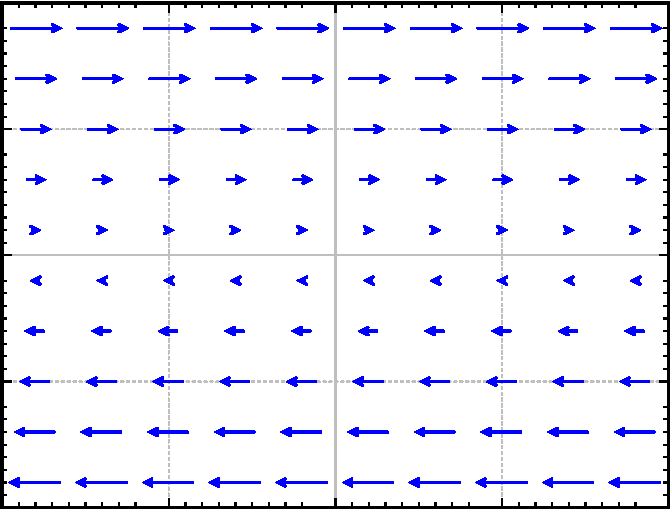
\includegraphics[width=2in]{figures/0100vectorfield}
\\
The solution does not move anywhere if $y = 0$.  When $y$ is positive,
the solution moves (with constant speed)
in the positive $x$ direction.  When $y$ is
negative, the solution moves (with constant speed) in the negative
$x$ direction.  It is not one of the behaviors we have seen.
\\
Note that the matrix has a double eigenvalue 0 and the general solution is
$x = C_1 t + C_2$ and $y = C_1$, which agrees with the
description above.
}

%\input ch-systems-fr.tex

%mbxSTARTIGNORE
%This makes contents fit if needed
%FIXMEevillayouthack
\addextraspacetotoc
%mbxENDIGNORE


%%%%%%%%%%%%%%%%%%%%%%%%%%%%%%%%%%%%%%%%%%%%%%%%%%%%%%%%%%%%%%%%%%%%%%%%%%%%%%

% Fourier series and PDEs chapter
\chapter{Séries de Fourier et équations différentielles partielles} \label{FS:chapter}

%%%%%%%%%%%%%%%%%%%%%%%%%%%%%%%%%%%%%%%%%%%%%%%%%%%%%%%%%%%%%%%%%%%%%%%%%%%%%%

\section{Équations avec conditions au bord} \label{bvp:section}

%\sectionnotes{2 lectures\EPref{, similar to \S3.8 in \cite{EP}}\BDref{,
%\S10.1 and \S11.1 in \cite{BD}}}

\subsection{Valeurs au bord}

Avant de s'attaquer aux séries de Fourier, on va étudier les problèmes \emph{à valeurs au bord\index{boundary value problem}}
 (ou \emph{à valeurs limites\index{endpoint problem}}).  On considère
\begin{equation*}
x'' + \lambda x = 0, \quad x(a) = 0, \quad x(b) = 0
\end{equation*}
pour une certaine constante $\lambda$, où $x(t)$ prend ses valeurs  $t$ dans l'intervalle 
$[a,b]$.
Précédemment, on a spécifié la valeur de la solution et de sa dérivée en un point. Maintenant, on veut spécifier la valeur de la solution à deux points différents. Lorsque $x=0$ est une solution, l'existence de la solution n'est pas problématique. Par contre, l'unicité de la solution est une autre question. La solution générale de  $x'' + \lambda x = 0$ a deux constantes arbitraires\footnote{%
On regarde la \subsectionref{subsection:fourfundamental}, ou l'\exampleref {example:expsecondorder} et l'\exampleref{example:sincossecondorder}.}.
C'est naturel (mais faux) de croire qu'exiger deux solutions garantit l'unicité. 

\begin{example}
On prend $\lambda = 1$,
$a=0$, $b=\pi$.  Ceci donne: 
\begin{equation*}
x'' + x = 0, \quad x(0) = 0, \quad x(\pi) = 0.
\end{equation*}
Alors, $x = \sin t$ est une autre solution  (qui s'ajoute à $x=0$) satisfaisant aux conditions limites. 
Il y a plus. Écrivons la solution générale de l'équation différentielle, qui est  $x= A \cos t + B \sin t$.
La condition $x(0) = 0$ implique que $A=0$.  La contrainte $x(\pi) = 0$ ne donne pas plus d'information lorsque $x = B \sin t$ satisfait déjà aux conditions limites. 
Par conséquent, il y a une infinité de solutions de la forme  $x = B \sin t$,
où $B$ est une constante arbitraire.  
\end{example}

\begin{example}
Posons maintenant $\lambda = 2$: 
\begin{equation*}
x'' + 2 x = 0, \quad x(0) = 0, \quad x(\pi) = 0.
\end{equation*}
Alors, la solution générale est
$x= A \cos ( \sqrt{2}\,t) + B \sin ( \sqrt{2}\,t)$.  La contrainte $x(0) = 0$ implique encore que $A = 0$.  On applique la seconde condition pour trouver 
$0=x(\pi) = B \sin ( \sqrt{2}\,\pi)$.
Lorsque $\sin ( \sqrt{2}\,\pi) \not= 0$, on obtient
$B = 0$.  
Donc, $x=0$ est l'unique solution à ce problème.
\end{example}

Que se passe-t-il ?  On aimerait savoir quelles constantes  $\lambda$ permettent une solution non nulle et l'on s'intéressera à trouver ces solutions. Ce problème est analogue  à trouver les valeurs propres et les vecteurs propres des matrices.

\subsection{Problèmes de valeurs propres}

Pour la théorie de base des séries de Fourier, on a besoin
des trois problèmes de valeurs propres suivants : 

\begin{equation} \label{bv:eq1}
x'' + \lambda x = 0, \quad x(a) = 0, \quad x(b) = 0 ,
\end{equation}
\begin{equation} \label{bv:eq2}
x'' + \lambda x = 0, \quad x'(a) = 0, \quad x'(b) = 0
\end{equation}
et
\begin{equation} \label{bv:eq3}
x'' + \lambda x = 0, \quad x(a) = x(b), \quad x'(a) = x'(b) .
\end{equation}
Un nombre $\lambda$ est appelé une
\emph{valeur propre \index{eigenvalue of a boundary value problem}}
de \eqref{bv:eq1}
(resp.\ \eqref{bv:eq2} ou \eqref{bv:eq3}) si et seulement si il existe une solution non nulle (non identiquement nulle) à \eqref{bv:eq1}
(resp.\ \eqref{bv:eq2} ou \eqref{bv:eq3})
donnée par un $\lambda$ spécifique. Une solution non nulle est appelée 
\emph{\myindex{fonction propre correspondante}}\index{corresponding eigenfunction}.

On note la similarité avec les valeurs propres et les vecteurs propres de matrices. La similarité n'est pas une simple coïncidence.  Par exemple, soit $L = -\frac{d^2}{{dt}^2}$ un opérateur linéaire.  Une fonction propre pour $L$ sera une fonction $x(t)$ non nulle telle que $Lx = \lambda x$, pour un certain $\lambda$, qui sera alors une valeur propre de l'opérateur $L$.

En d'autres mots, on pense à l'équation différentielle comme à un opérateur différentiel, et à une fonction $x(t)$
comme à un vecteur avec une infinité de composantes (une pour chaque $t$).
Une fonction propre sera une fonction non nulle $x$ qui satisfait à 
$(L- \lambda)x = 0$. Il y a beaucoup de formalisme provenant de l'algèbre linéaire qui s'applique ici, mais on ne poursuivra pas cette réflexion trop loin.  

\begin{example} \label{bvp:eig1ex}
Trouvons les valeurs propres et les fonctions propres de 
\begin{equation*}
x'' + \lambda x = 0, \quad x(0) = 0, \quad x(\pi) = 0 .
\end{equation*}

%For reasons that will be clear from the computations,
On doit considérer chacun des cas suivants séparément, $\lambda > 0$, $\lambda = 0$, $\lambda < 0$, puisque la solution générale est différente dans les trois cas.
D'abord, on suppose que $\lambda > 0$.  Alors, la solution générale à $x''+\lambda x = 0$ est
\begin{equation*}
x = A \cos ( \sqrt{\lambda}\, t) + B \sin ( \sqrt{\lambda}\, t).
\end{equation*}
La condition $x(0) = 0$ implique immédiatement que $A = 0$.
Ensuite,
\begin{equation*}
0 = x(\pi) = B \sin ( \sqrt{\lambda}\, \pi ) .
\end{equation*}
Si $B$ est nul, alors $x$ est une solution nulle. Alors, pour obtenir une solution non nulle, on doit avoir que $\sin ( \sqrt{\lambda}\, \pi) = 0$.  Donc,
$\sqrt{\lambda}\, \pi$ doit être un entier multiple de $\pi$.  En d'autres mots,
 $\sqrt{\lambda} = k$ pour un entier positif $k$.
Ainsi, les valeurs propres positives sont 
$k^2$ pour tous les entiers $k \geq 1$.  Les fonctions propres correspondantes peuvent être vues comme $x=\sin (k t)$.  Tout comme les vecteurs propres, les multiples d'une fonction propre sont des fonctions propres. 

On suppose que $\lambda = 0$.  Dans ce cas, l'équation est $x'' = 0$,
et sa solution générale est $x = At + B$.  La condition  $x(0) = 0$ implique que 
 $B=0$, et $x(\pi) = 0$ implique que $A = 0$, ce qui signifie que $\lambda
= 0$ n'est \emph{pas} une valeur propre.

Finalement, on suppose que $\lambda < 0$. Dans ce cas, on a la solution générale\footnote{%
Rappelons que 
$\cosh s = \frac{1}{2}(e^s+e^{-s})$
et
$\sinh s = \frac{1}{2}(e^s-e^{-s})$.  En exercice, faites à nouveau les calculs avec la solution générale écrite comme 
$x = A e^{\sqrt{-\lambda}\, t} + B e^{-\sqrt{-\lambda}\, t}$ (pour différents  $A$ et $B$ évidemment).}
\begin{equation*}
x = A \cosh ( \sqrt{-\lambda}\, t) + B \sinh ( \sqrt{-\lambda}\, t ) .
\end{equation*}
Si $x(0) = 0$, ça implique que $A = 0$ (on se rappelle que $\cosh 0 = 1$ et $\sinh 0 =
0$).  Alors, la solution devrait être $x = B \sinh ( \sqrt{-\lambda}\, t )$ et devrait satisfaire à 
$x(\pi) = 0$, ce qui est possible uniquement si $B$ est nul. Pourquoi? Parce que 
$\sinh \xi$ est seulement zéro lorsque $\xi=0$.  On devrait calculer sinh pour voir ce fait. On peut aussi le voir de la définition de sinh. On obtient $0 = \sinh \xi = \frac{e^\xi -
e^{-\xi}}{2}$. Donc, $e^\xi = e^{-\xi}$, ce qui implique que $\xi = -\xi$, ce qui est seulement vrai si $\xi=0$. Par conséquent, il n'y a pas de valeurs propres négatives.  

En somme, les valeurs propres et les fonctions propres correspondantes sont 
\begin{equation*}
\lambda_k = k^2 \quad \text{avec fonction propre} \quad x_k = \sin (k t)
\quad \text{pour tous les entiers } k \geq 1 .
\end{equation*}
\end{example}

\begin{example}
Calculons les valeurs propres et les fonctions propres de 
\begin{equation*}
x'' + \lambda x = 0, \quad x'(0) = 0, \quad x'(\pi) = 0 .
\end{equation*}

Encore une fois, on doit considérer séparément  les trois cas suivants: $\lambda > 0$, $\lambda = 0$, $\lambda
< 0$.
D'abord, on suppose que $\lambda > 0$.
La solution générale est alors 
$x = A \cos ( \sqrt{\lambda}\, t) + B \sin ( \sqrt{\lambda}\, t)$.  Sa dérivée est: 
\begin{equation*}
x' = -A\sqrt{\lambda}\, \sin ( \sqrt{\lambda}\, t) + B\sqrt{\lambda}\,
\cos (\sqrt{\lambda}\, t) .
\end{equation*}
La condition $x'(0) = 0$ implique immédiatement que  $B = 0$.
Ensuite,
\begin{equation*}
0 = x'(\pi) = -A\sqrt{\lambda}\, \sin ( \sqrt{\lambda}\, \pi) .
\end{equation*}
Encore une fois,  $A$ ne peut pas être nul si  $\lambda$ est une valeur propre, et $\sin ( \sqrt{\lambda}\, \pi)$ est identiquement nul lorsque
$\sqrt{\lambda} = k$,  où $k$ est un nombre entier positif.
Donc, les valeurs propres positives sont encore 
$k^2$ pour tous les entiers $k \geq 1$, et les fonctions propres correspondantes peuvent être prises comme  $x=\cos (k t)$.

Maintenant, on suppose que  $\lambda = 0$.  Dans ce cas, l'équation est $x'' = 0$,
et la solution générale est $x = At + B$ so $x' = A$.  La condition 
$x'(0) = 0$ implique que 
$A=0$.  La condition $x'(\pi) = 0$ implique aussi que  $A=0$.
Ainsi, $B$ pourrait être n'importe quoi (choisissons 1). Alors, $\lambda = 0$
est une valeur propre, et $x=1$ est la fonction propre correspondante. 

Finalement, soit $\lambda < 0$.  Dans ce cas, la solution générale est 
$x = A \cosh ( \sqrt{-\lambda}\, t) + B \sinh ( \sqrt{-\lambda}\, t)$
et
\begin{equation*}
x' = A\sqrt{-\lambda}\, \sinh ( \sqrt{-\lambda}\, t)
+ B\sqrt{-\lambda}\, \cosh ( \sqrt{-\lambda}\, t ) .
\end{equation*}
On a déjà vu (avec les rôles de  $A$ et de $B$ inversés) que, pour que cette expression soit  nulle à $t=0$ et $t=\pi$, on doit avoir $A=B=0$. Ainsi, il n'y a pas de valeur propre négative. 

En somme, les valeurs propres positives et leurs fonctions propres correspondantes sont
\begin{equation*}
\lambda_k = k^2 \quad \text{avec fonction propre} \quad x_k = \cos (k t)
\quad \text{pour tous les entiers } k \geq 1 ,
\end{equation*}
et, de plus, il y a une autre valeur propre: 
\begin{equation*}
\lambda_0 = 0 \qquad \text{avec une fonction propre} \qquad x_0 = 1.
\end{equation*}
\end{example}

Le problème suivant est celui qui a mené à la série de Fourier générale.

\begin{example} \label{bvp-periodic:example}
Calculons les valeurs propres et les fonctions propres de 
\begin{equation*}
x'' + \lambda x = 0, \quad x(-\pi) = x(\pi), \quad x'(-\pi) = x'(\pi) .
\end{equation*}
On n'a pas de valeur spécifique de fonction ou de dérivée aux extrémités, mais elles sont les mêmes au début et à la fin de l'intervalle. 

On va passer le cas $\lambda < 0$.  Les calculs sont les mêmes que précédemment, et l'on trouve encore qu'il n'y a pas de valeur propre négative. 

Pour $\lambda = 0$, la solution générale est $x = At + B$.  La condition
$x(-\pi) = x(\pi)$ implique que $A=0$ ($A\pi + B = -A\pi +B$ implique que $A=0$).
La seconde condition $x'(-\pi) = x'(\pi)$ ne dit rien à propos de $B$, et donc
$\lambda=0$ est une valeur propre avec les fonctions propres correspondantes $x=1$.

Pour $\lambda > 0$, on a que 
$x = A \cos ( \sqrt{\lambda}\, t ) + B \sin ( \sqrt{\lambda}\, t)$.
Maintenant,
\begin{equation*}
\underbrace{A \cos (-\sqrt{\lambda}\, \pi) + B \sin (-\sqrt{\lambda}\,
\pi)}_{x(-\pi)}
=
\underbrace{A \cos (  \sqrt{\lambda}\, \pi ) + B \sin ( \sqrt{\lambda}\,
\pi)}_{x(\pi)} .
\end{equation*}
On se rappelle que $\cos (- \theta) = \cos (\theta)$ et
$\sin (-\theta) = - \sin (\theta)$. Donc,
\begin{equation*}
A \cos (\sqrt{\lambda}\, \pi) - B \sin ( \sqrt{\lambda}\, \pi)
=
A \cos (\sqrt{\lambda}\, \pi) + B \sin ( \sqrt{\lambda}\, \pi).
\end{equation*}
Donc, ou bien $B=0$, ou bien $\sin ( \sqrt{\lambda}\, \pi) = 0$.
De manière semblable à l'exemple précédent (exercice), si l'on dérive $x$ et qu'on le remplace dans la seconde condition, on trouve que $A=0$ ou que $\sin ( \sqrt{\lambda}\, \pi) = 0$.
Ainsi, à moins que $A$ et $B$ soient tous deux nuls (ce qu'on ne veut pas), on doit avoir $\sin ( \sqrt{\lambda}\, \pi ) = 0$.  Donc, $\sqrt{\lambda}$
est un entier, et les valeurs propres sont encore $\lambda = k^2$ pour un entier
 $k \geq 1$. Dans ce cas, toutefois,  
$x = A \cos (k t) + B \sin (k t)$ est une fonction propre pour tout $A$ et pour tout $B$.
Par conséquent, on a deux fonctions propres linéairement indépendantes: $\sin (kt)$ et $\cos (kt)$.

On se rappelle que, pour une matrice, on peut aussi avoir deux vecteurs propres correspondant à une valeur propre simple si la valeur propre est répétée. 

En somme, les valeurs propres et les fonctions propres sont 
\begin{align*}
& \lambda_k = k^2 & & \text{avec fonctions propres} & &
\cos (k t) \quad \text{et}\quad  \sin (k t)
 & & \text{pour tous les entiers } k \geq 1 , \\
& \lambda_0 = 0 & & \text{avec fonction propre} & & x_0 = 1.
\end{align*}
\end{example}

\subsection{Orthogonalité des fonctions propres}

Une chose qui sera très utile dans la prochaine section est la propriété d'\emph{\myindex{orthogonalité}} des fonctions propres. C'est analogue aux vecteurs propres d'une matrice. Une matrice est 
\emph{symétrique\index{symmetric matrix}}
si $A = A^T$ (est égale à sa transposée).
\emph{Les vecteurs propres de deux valeurs propres distinctes d'une matrice symétrique sont orthogonaux.}
%That symmetry is required.  
%We will not prove this fact here.
L'opérateur différentiel que l'on considère agit plutôt comme  une matrice symétrique. Ainsi, on obtient le théorème suivant.  

%\medskip
%
%Suppose $\lambda_1$ and $\lambda_2$ are two distinct eigenvalues of $A$
%and $\vec{v}_1$ and $\vec{v}_2$ are the corresponding eigenvectors.  Then
%we of course have that $A \vec{v}_1 = \lambda_1 \vec{v}_1$ and
%$A \vec{v}_2 = \lambda_2 \vec{v}_2$.
%\begin{equation*}
%\langle A \vec{v}_1 , \vec{v}_2 \rangle = \lambda_1 \langle \vec{v}_1 , \vec{v}_2 \rangle
%\qquad
%\langle A \vec{v}_2 , \vec{v}_1 \rangle = \lambda_2 \langle \vec{v}_2 , \vec{v}_1 \rangle
%\end{equation*}
%
%\begin{equation*}
%\langle A \vec{v}_1 , \vec{v}_2 \rangle -
%\langle A \vec{v}_2 , \vec{v}_1 \rangle 
%=
%(\lambda_1 - \lambda_2 ) \langle \vec{v}_1 , \vec{v}_2 \rangle
%\end{equation*}
%
%\begin{equation*}
%\langle (A-A^T) \vec{v}_1 , \vec{v}_2 \rangle
%=
%(\lambda_1 - \lambda_2 ) \langle \vec{v}_1 , \vec{v}_2 \rangle
%\end{equation*}

\begin{theorem} \label{bvp:orthogonaleigen}
Soit  $x_1(t)$ et $x_2(t)$ deux fonctions propres du problème 
\eqref{bv:eq1}, \eqref{bv:eq2} ou \eqref{bv:eq3}
pour deux valeurs propres distinctes $\lambda_1$ et $\lambda_2$. Alors, elles sont
\emph{orthogonales \index{orthogonal!functions}}
dans le sens que
\begin{equation*}
\int_a^b x_1(t) x_2(t) \,dt = 0 .
\end{equation*}
\end{theorem}

La terminologie vient du fait que l'intégrale est un type de produit scalaire. On précisera ce sujet dans la prochaine section. Le théorème a une preuve  très petite, élégante et éclairante qui est présentée ici.  
D'abord, on a les deux équations suivantes : 
\begin{equation*}
x_1'' + \lambda_1 x_1 = 0
\qquad \text{et} \qquad
x_2'' + \lambda_2 x_2 = 0.
\end{equation*}
On multiplie la première par $x_2$ et la seconde par $x_1$, et l'on substitue pour obtenir 
\begin{equation*}
(\lambda_1 - \lambda_2) x_1 x_2 = x_2'' x_1 - x_2 x_1'' .
\end{equation*}
Maintenant, on intègre des deux côtés de l'équation: 
\begin{equation*}
\begin{split}
(\lambda_1 - \lambda_2) \int_a^b x_1 x_2 \,dt
& =
\int_a^b x_2'' x_1 - x_2 x_1'' \,dt \\
& =
\int_a^b \frac{d}{dt} \left( x_2' x_1 - x_2 x_1' \right) \,dt \\
& =
\Bigl[ x_2' x_1 - x_2 x_1' \Bigr]_{t=a}^b
= 0 .
\end{split}
\end{equation*}
La dernière égalité tient en raison des conditions aux limites. Par exemple, si l'on considère \eqref{bv:eq1}, on a  $x_1(a) = x_1(b) = x_2(a) = x_2(b) = 0$, et alors $x_2' x_1 - x_2 x_1'$ est nul pour $a$ et pour $b$.
Lorsque $\lambda_1 \not= \lambda_2$, le théorème suit.

\begin{exercise}[facile]
Terminez la preuve du théorème (vérifiez la dernière égalité de la preuve) pour les cas \eqref{bv:eq2} et \eqref{bv:eq3}.
\end{exercise}

La fonction $\sin (n t)$ est une fonction propre pour l'équation 
$x''+\lambda x = 0$, $x(0) = 0$, $x(\pi) = 0$. 
Donc, pour les entiers positifs $n$ et $m$:  
\begin{equation*}
\int_{0}^\pi \sin (mt) \sin (nt) \,dt = 0 ,
\quad
\text{lorsque } m \not = n.
\end{equation*}
De manière similaire,
\begin{equation*}
\int_{0}^\pi \cos (mt) \cos (nt) \,dt = 0 ,
\quad
\text{lorsque } m \not = n,
\qquad \text{et} \qquad
\int_{0}^\pi  \cos (nt) \,dt = 0 .
\end{equation*}
Et finalement, on obtient aussi
\begin{equation*}
\int_{-\pi}^\pi \sin (mt) \sin (nt) \,dt = 0 ,
\quad
\text{lorsque } m \not = n, 
\qquad \text{et} \qquad
\int_{-\pi}^\pi  \sin (nt) \,dt = 0 ,
\end{equation*}
\begin{equation*}
\int_{-\pi}^\pi \cos (mt) \cos (nt) \,dt = 0 ,
\quad
\text{lorsque } m \not = n,
\qquad \text{et} \qquad
\int_{-\pi}^\pi  \cos (nt) \,dt = 0 ,
\end{equation*}
et
\begin{equation*}
\int_{-\pi}^\pi \cos (mt) \sin (nt) \,dt = 0 
\qquad \text{(même si $m=n$).}
\end{equation*}

%\medskip
%
%The theorem is also true when different boundary conditions are applied as
%well.  For example, if we require $x'(a) = x'(b) = 0$, or
%$x(a) = x'(b) = 0$, or
%$x'(a) = x(b) = 0$.  See the proof.


%By what we have seen previously we apply the theorem to find the integrals
%\begin{equation*}
%\int_{-\pi}^\pi \sin (mt) \sin (nt) \,dt = 0 \qquad \text{and} \qquad
%\int_{-\pi}^\pi \cos (mt) \cos (nt) \,dt = 0 ,
%\end{equation*}
%when $m \not = n$, and 
%\begin{equation*}
%\int_{-\pi}^\pi \sin (mt) \cos (nt) \,dt = 0 ,
%\end{equation*}
%for all $m$ and $n$.

\subsection{Alternative de Fredholm}

On arrive maintenant à un théorème très utile des équations différentielles. Le théorème pourrait être plus général que ce qu'on présentera, mais, pour les objectifs actuels, il sera suffisant. On en donnera une version un peu plus générale plus tard.

\begin{theorem}[Alternative de Fredholm\footnote{%
Nommée d'après le mathématicien suédois
\href{https://en.wikipedia.org/wiki/Fredholm}{Erik Ivar Fredholm}
(1866-1927).}]\index{Fredholm alternative!simple case}
\label{thm:fredholmsimple}
Exactement l'une des affirmations suivantes est vraie.
Soit
\begin{equation} \label{simpfredhomeq}
x'' + \lambda x = 0, \quad x(a) = 0, \quad x(b) = 0
\end{equation}
a une solution non nulle, soit
\begin{equation} \label{simpfrednonhomeq}
x'' + \lambda x = f(t), \quad x(a) = 0, \quad x(b) = 0
\end{equation}
a une solution unique pour toutes les fonctions $f$ continues sur $[a,b]$.
\end{theorem}

Le théorème est également vrai pour les autres types de
conditions au bord que nous avons considérées.
Le théorème veut dire que si  $\lambda$ n'est pas une valeur propre, l'équation non homogène  \eqref{simpfrednonhomeq} a une solution unique pour tous les côtés droits. Autrement dit, si $\lambda$ est une valeur propre, alors  
\eqref{simpfrednonhomeq} n'a pas besoin d'avoir une solution pour tous les $f$,
et, en plus, même s'il y a une solution, la solution n'est pas unique.

Nous voulons également renforcer l'idée que les opérateurs différentiels linéaires ont beaucoup en commun avec les matrices. Il n'est donc pas surprenant qu'il existe une version de dimension finie de l'alternative de Fredholm pour les matrices  également.  On a $A$ une matrice $n \times n$. L'alternative de Fredholm dit que $(A-\lambda I) \vec{x} = \vec{0}$ a une solution non triviale, ou que $(A-\lambda I) \vec{x} = \vec{b}$ a une solution unique pour tout $\vec{b}$.

Beaucoup d'intuition de l'algèbre linéaire peut être appliquée aux opérateurs différentiels linéaires, mais il faut bien sûr être prudent. Par exemple, une différence que nous avons déjà vue est qu'en général un opérateur différentiel
aura une infinité de valeurs propres, tandis qu'une matrice n'en a qu'un nombre fini.


\subsection{Application}

Considérons une application physique. On suppose avoir un élastique très tendu qui tourne rapidement ou une corde de densité linéaire uniforme $\rho$, par exemple, en
$\unitfrac{kg}{m}$.
Mettons ce problème dans un plan $xy$ avec $x$ et $y$ en mètres. L'axe des $x$ représente la position de la corde. La corde tourne, et la vitesse angulaire est $\omega$, mesurée en $\unitfrac{radians}{s}$.
Imaginez que l'entièreté du plan $xy$ tourne à une vitesse angulaire  $\omega$.
De cette manière, la corde reste dans le plan $xy$, et $y$ mesure sa déviation par rapport à la position d'équilibre, $y=0$, sur l'axe des $x$.
Ainsi, le graphe de $y$ donne la forme de la corde.
On considère une corde idéale qui n'a pas de volume, juste une courbe mathématique. On suppose que la tension de la corde est une constante $T$ en newtons.
%If we take a small segment and we look at the tension at the endpoints, we
%see that this force is tangential and we will assume that the magnitude is
%the same at both end points.  Hence the magnitude
%is constant everywhere and we will
%call its magnitude $T$.
En supposant que la déviation est petite, nous pouvons utiliser la deuxième loi de Newton (nous n'en faisons pas la démonstration) pour obtenir l'équation suivante: 
\begin{equation*}
T y'' + \rho \omega^2 y = 0 .
\end{equation*}
Pour vérifier les unités, notez que les unités de $y''$ sont $\unitfrac{m}{m^2}$, lorsqu'on dérive par rapport à $x$.

La corde  est de longueur $L$ (en mètres) et est fixée aux deux extrémités. Alors, $y(0) = 0$ et $y(L) = 0$.  Voir la \figureref{bvp:whirstringfig}.

\begin{myfig}
\capstart
\inputpdft{bvp-whirstring}
\caption{Corde tournante.\label{bvp:whirstringfig}}
\end{myfig}

On réécrit l'équation: 
$y'' + \frac{\rho \omega^2}{T} y = 0$.
La configuration est semblable à l'\exampleref{bvp:eig1ex}, sauf que  
la longueur de l'intervalle est $L$ plutôt que $\pi$. On cherche les valeurs propres de  $y'' + \lambda y = 0, y(0) = 0, y(L) = 0$, où
$\lambda = \frac{\rho \omega^2}{T}$.  Comme précédemment, il n'y a pas de valeur propre négative. Avec $\lambda > 0$,
la solution générale à cette équation est $y = A \cos (  \sqrt{\lambda} \,x ) + B
\sin ( \sqrt{\lambda} \,x )$.  La condition $y(0) = 0$ implique que $A = 0$ comme précédemment. La condition $y(L) = 0$ implique que
$\sin ( \sqrt{\lambda} \, L) = 0$, et ainsi
$\sqrt{\lambda} \, L = k \pi$  pour un certain entier $k > 0$, alors
\begin{equation*}
\frac{\rho \omega^2}{T} = \lambda = \frac{k^2 \pi^2}{L^2} .
\end{equation*}

Qu'est-ce que cela dit sur la forme de la corde? Cela dit que, pour tous les paramètres $\rho$, $\omega$, $T$ qui ne satisfont pas à cette condition, la corde demeure dans sa position d'équilibre, $y=0$.  Mais lorsque 
$\frac{\rho \omega^2}{T} = \frac{k^2 \pi^2}{L^2}$, alors la corde \myquote{sortira} d'une distance $B$. On ne peut pas calculer $B$ avec les informations que l'on a. 

On suppose que  $\rho$ et $T$ sont fixes et l'on fait varier $\omega$.
Pour la plupart des valeurs de $\omega$, la corde est à l'état d'équilibre. Lorsque la vitesse angulaire  $\omega$ atteint une valeur $\omega = \frac{k \pi \sqrt{T}}{L\sqrt{\rho}}$, alors la corde sort et a la forme d'une vague sinusoïdale croisant l'axe des 
$x$ $k-1$ fois entre les extrémités. Par exemple, à $k=1$, la corde ne croise pas l'axe des $x$, et la forme ressemble à la \figurevref{bvp:whirstringfig} plus haut.
D'un autre côté, lorsque  $k=3$, la corde croise l'axe des $x$ deux fois. On le voit dans la  \figurevref{bvp:whirstring2fig}.
Lorsque $\omega$ change encore, la corde retourne à sa position d'équilibre. Plus la vitesse angulaire est élevée, plus la corde croisera l'axe des  $x$ lorsqu'elle sortira.

\begin{myfig}
\capstart
\inputpdft{bvp-whirstring2}
\caption{Corde tournante à la troisième valeur propre ($k=3$).\label{bvp:whirstring2fig}}
\end{myfig}

Pour un autre exemple, si l'on a une corde à sauter qui tourne (alors $k=1$ lorsqu'elle sort \myquote{complètement}) et que l'on tire sur les extrémités pour augmenter la tension, alors la vitesse augmente pour que la corde reste \myquote{sortie}.
 

\subsection{Exercices}

Astuce pour les exercices suivants:  Notez que lorsque  $\lambda > 0$, alors
$\cos \bigl( \sqrt{\lambda}\, (t - a) \bigr)$
et $\sin  \bigl( \sqrt{\lambda}\, (t - a) \bigr)$
sont aussi des solutions de l'équation homogène. 

\begin{exercise}
Calculez toutes les valeurs propres et toutes les fonctions propres de 
$x'' + \lambda x = 0, ~ x(a) = 0, ~ x(b) = 0$ (supposez que $a < b$).
\end{exercise}

\begin{exercise}
Calculez toutes les valeurs propres et toutes les fonctions propres de 
$x'' + \lambda x = 0, ~ x'(a) = 0, ~ x'(b) = 0$ (supposez que $a < b$).
\end{exercise}

\begin{exercise}
Calculez toutes les valeurs propres et toutes les fonctions propres de 
$x'' + \lambda x = 0, ~ x'(a) = 0, ~ x(b) = 0$ (supposez que $a < b$).
\end{exercise}

\begin{exercise}
Calculez toutes les valeurs propres et toutes les fonctions propres de 
$x'' + \lambda x = 0, ~ x(a) = x(b), ~ x'(a) = x'(b)$ (supposez que $a < b$).
\end{exercise}

\begin{exercise}
On ne considérera pas le cas  $\lambda < 0$ pour la valeur à l'extrêmité du problème f
$x'' + \lambda x = 0, ~ x(-\pi) = x(\pi), ~ x'(-\pi) = x'(\pi)$.
Terminez le calcul et montrez qu'il n'y a pas de valeur propre négative. 
\end{exercise}

\setcounter{exercise}{100}

\begin{exercise}
Considérez une corde, de longueur 2, de densité linéaire de 0,1 et de tension 3,  qui tourne. Trouvez la plus petite vitesse angulaire permettant à la corde de sortir. 
\end{exercise}
\exsol{%
$\omega = \pi \sqrt{\frac{15}{2}}$
}

\begin{exercise}
Supposez que $x'' + \lambda x = 0$ et $x(0)=1$, $x(1) = 1$.
Trouvez tous les $\lambda$ pour lesquels il y a plus d'une solution. Trouvez aussi les solutions correspondantes (seulement pour les valeurs propres). 
\end{exercise}
\exsol{%
$\lambda_k = 4 k^2 \pi^2$ pour $k = 1,2,3,\ldots$
\quad
$x_k =  \cos (2k\pi t) + B \sin (2k\pi t)$ \quad (pour tout $B$)
}

\begin{exercise}
Supposez que $x'' + x = 0$ et $x(0)=0$, $x'(\pi) = 1$.
Trouvez toute(s) les solution(s) si elles existent.  
\end{exercise}
\exsol{%
$x(t) = - \sin(t)$
}

\begin{exercise}
Considerez
$x' + \lambda x = 0$ et $x(0)=0$, $x(1) = 0$.  Pourquoi il n'y a pas de valeurs propres? Pourquoi toutes les équation de premier ordre avec deux conditions au bord comme ci-haut n'ont pas de valeurs propres? 
\end{exercise}
\exsol{%
La solution générale est $x = C e^{-\lambda t}$.  Depuis que $x(0) = 0$ alors $C=0$, et alors $x(t) = 0$.
Ainsi, la solution est toujours identiquement nulle. Une condition est toujours suffisante pour garantir une solution unique pour une équation de premier ordre. 
}

\begin{exercise}[défi]
Supposez que $x''' + \lambda x = 0$ et $x(0)=0$, $x'(0) = 0$, $x(1) = 0$.
Supposez que  $\lambda > 0$.  Trouvez une équation à laquelle toutes les valeurs propres satisferont. 
Astuce : Notez que $-\sqrt[3]{\lambda}$ est une racine de $r^3+\lambda = 0$.
\end{exercise}
\exsol{%
$\frac{\sqrt{3}}{3} e^{\frac{-3}{2}\sqrt[3]{\lambda}}
- \frac{\sqrt{3}}{3} \cos \bigl( \frac{\sqrt{3}\, \sqrt[3]{\lambda}}{2} \bigr)
+ \sin \bigl( \frac{\sqrt{3}\, \sqrt[3]{\lambda}}{2}\bigr) = 0$
}

%%%%%%%%%%%%%%%%%%%%%%%%%%%%%%%%%%%%%%%%%%%%%%%%%%%%%%%%%%%%%%%%%%%%%%%%%%%%%%

\sectionnewpage
\section{Séries trigonométriques} \label{ts:section}


\subsection{Fonctions périodiques et motivations}

Afin de motiver l'étude des séries de Fourier, considérons le problème suivant:
\begin{equation} \label{ts:deq}
x'' + \omega_0^2 x = f(t) ,
\end{equation}
pour une certaine fonction périodique $f(t)$.
On a déjà résolu
\begin{equation} \label{ts:deqcos}
x'' + \omega_0^2 x = F_0 \cos ( \omega t) .
\end{equation}
Une manière de résoudre \eqref{ts:deq} est de décomposer $f(t)$ comme une somme de cosinus (et de sinus) et de résoudre plusieurs problèmes de la forme  \eqref{ts:deqcos}.  On utilise ensuite le principe de superposition pour additionner toutes les solutions obtenues pour obtenir la solution de \eqref{ts:deq}.

Avant de procéder, parlons un peu plus en détail des fonctions périodiques. 
Une fonction est  \emph{\myindex{périodique}} avec période $P$ si
$f(t) = f(t+P)$ pour tous $t$.  On dit alors que $f(t)$ est $P$-périodique.
On note qu'une fonction $P$-périodique est aussi $2P$-périodique, $3P$-périodique
et ainsi de suite.
Par exemple, $\cos (t)$ et $\sin (t)$ sont
$2\pi$-périodiques.  Alors $\cos (kt)$ et $\sin (kt)$ pour tous les entiers $k$.  Les fonctions constantes sont des exemples extrêmes: elles sont périodiques pour n'importe quelle période (exercice). 

Normalement, on commence avec la fonction $f(t)$ définie sur un certain intervalle $[-L,L]$,
et l'on veut
\emph{prolonger $f(t)$ périodiquement}\index{extend periodically}\index{periodic extension}
pour qu'elle devienne une fonction $2L$-périodique.  On fait cette extension en définissant une nouvelle fonction $F(t)$
telle que pour tout $t$ dans $[-L,L]$, $F(t) = f(t)$.  Pour tout $t$ dans $[L,3L]$,
on définit $F(t) = f(t-2L)$, pour $t$ dans $[-3L,-L]$, $F(t) = f(t+2L)$, et ainsi de suite.
Pour faire ce travail, on a besoin de $f(-L) = f(L)$.
On pourrait aussi commencer avec $f$
défini seulement sur un demi-intervalle ouvert $(-L,L]$ et l'on définit $f(-L) = f(L)$.

\begin{example}
Définissons  $f(t) = 1-t^2$ sur $[-1,1]$.  Maintenant, on prolonge $f(t)$ périodiquement pour obtenir une fonction 2-périodique.  Voir la figure~\figureref{ts:perextofinvertedparabolafig}.
\begin{myfig}
\capstart
\diffyincludegraphics{width=3in}{width=4.5in}{ts-perextofinvertedparabola}
\caption{Prolongement 2-périodique de la fonction 
$1-t^2$.\label{ts:perextofinvertedparabolafig}}
\end{myfig}
\end{example}

On doit faire attention à bien distinguer $f(t)$ de ses différents prolongements.  Une erreur commune est de supposer que la formule pour $f(t)$ fonctionne toujours pour ses prolongements. Il faut être particulièrement prudent lorsque $f(t)$ est périodique, mais avec une période différente.

\begin{exercise}
Définissez $f(t) = \cos t$ sur $[\nicefrac{-\pi}{2},\nicefrac{\pi}{2}]$.  Prenez l'extension $\pi$-périodique et esquissez le graphique. Comparez avec le graphique de $\cos t$.
\end{exercise}

\subsection{Produit scalaire et décomposition de vecteurs propres }

Comme on l'a remarqué précédemment, lorsque $A$ est une \emph{\myindex{matrice symétrique}},
c'est-à-dire lorsque $A^T = A$, les vecteurs propres de $A$ sont orthogonaux. Ici, le mot 
\emph{orthogonal}\index{orthogonal!vectors} signifie que si $\vec{v}$ et $\vec{w}$ sont deux vecteurs propres de $A$ pour des valeurs propres distinctes, alors $\langle \vec{v} , \vec{w} \rangle = 0$.
Dans ce cas, le produit scalaire  $\langle \vec{v} , \vec{w} \rangle$
est le \emph{\myindex{produit scalaire à dimensions finies}}, que l'on peut calculer comme $\vec{v}^T\vec{w}$.

Pour décomposer un vecteur $\vec{v}$ en termes de vecteurs multuellement orthogonaux  $\vec{w}_1$ et $\vec{w}_2$ on écrit
\begin{equation*}
\vec{v} = a_1 \vec{w}_1  + a_2 \vec{w}_2 .
\end{equation*}
On trouve la formule pour $a_1$ et $a_2$. D'abord, on calcule 
\begin{equation*}
\langle \vec{v} , \vec{w_1} \rangle
=
\langle a_1 \vec{w}_1  + a_2 \vec{w}_2 , \vec{w_1} \rangle
=
a_1 \langle \vec{w}_1 , \vec{w_1} \rangle
+
a_2 \underbrace{\langle \vec{w}_2 , \vec{w_1} \rangle}_{=0}
=
a_1 \langle \vec{w}_1 , \vec{w_1} \rangle .
\end{equation*}
Ensuite,
\begin{equation*}
a_1 = 
\frac{\langle \vec{v} , \vec{w_1} \rangle}{
\langle \vec{w}_1 , \vec{w_1} \rangle} .
\end{equation*}
De manière similaire
\begin{equation*}
a_2 = 
\frac{\langle \vec{v} , \vec{w_2} \rangle}{
\langle \vec{w}_2 , \vec{w_2} \rangle} .
\end{equation*}
(Vous avez possiblement vu cette formule dans un cours d'algèbre linéaire.)

\begin{example}
Écrivons 
$\vec{v} = \left[ \begin{smallmatrix} 2 \\ 3 \end{smallmatrix} \right]$
comme une combinaison linéaire de 
$\vec{w_1} = \left[ \begin{smallmatrix} 1 \\ -1 \end{smallmatrix} \right]$
et
$\vec{w_2} = \left[ \begin{smallmatrix} 1 \\ 1 \end{smallmatrix} \right]$.

D'abord, on note que $\vec{w}_1$ et $\vec{w}_2$ sont orthogonaux, puisque 
 $\langle \vec{w}_1 , \vec{w}_2 \rangle = 1(1) + (-1)1 = 0$.
Alors
\begin{align*}
& a_1 = 
\frac{\langle \vec{v} , \vec{w_1} \rangle}{
\langle \vec{w}_1 , \vec{w_1} \rangle}
=
\frac{2(1) + 3(-1)}{1(1) + (-1)(-1)} = \frac{-1}{2} ,
\\
& a_2 = 
\frac{\langle \vec{v} , \vec{w_2} \rangle}{
\langle \vec{w}_2 , \vec{w_2} \rangle}
=
\frac{2 + 3}{1 + 1} = \frac{5}{2} .
\end{align*}
Ainsi,
\begin{equation*}
\begin{bmatrix} 2 \\ 3 \end{bmatrix}
=
\frac{-1}{2}
\begin{bmatrix} 1 \\ -1 \end{bmatrix}
+
\frac{5}{2}
\begin{bmatrix} 1 \\ 1 \end{bmatrix} .
\end{equation*}
\end{example}

\subsection{Séries trigonométriques}

Plutôt que décomposer un vecteur en termes de vecteurs propres d'une matrice, on va décomposer une fonction en termes de fonctions propres associées à un problème de valeur propre. Le problème de valeur propre qu'on utilise pour les séries de Fourier est 
\begin{equation*}
x'' + \lambda x = 0, \quad x(-\pi) = x(\pi), \quad x'(-\pi) = x'(\pi) .
\end{equation*}
Nous avons calculé les fonctions propres dans l'exemple~\ref{bvp-periodic:example}:t 1, $\cos (k t)$,
$\sin (k t)$.  Ainsi, on veut trouver une représentation d'une fonction 
$2\pi$-périodique $f(t)$ de la forme suivante: 
\begin{equation*}
\mybxbg{~~
f(t) = \frac{a_0}{2} +
\sum_{n=1}^\infty a_n \cos (n t) + b_n \sin (n t) .
~~}
\end{equation*}
Cette série s'appelle une  \emph{\myindex{série de Fourier}}%
\footnote{Nommée d'après le mathématicien français
\href{https://en.wikipedia.org/wiki/Joseph_Fourier}{Jean Baptiste Joseph Fourier}
(1768--1830).} ou une
\emph{\myindex{série trigonométrique}} pour $f(t)$.
Par convention, on écrit le coefficient de la fonction propre 1 comme $\frac{a_0}{2}$. On peut y penser comme $1 = \cos (0t)$.

Comme pour les matrices, on veut trouver une  \emph{\myindex{projection}}
de $f(t)$ sur un sous-espace donné par les fonctions propres. Alors on veut définir le  \emph{\myindex{produit scalaire d'une fonction}}.  Par exemple, pour trouver $a_n$ on veut calculer $\langle \, f(t) \, , \, \cos (nt) \, \rangle$.
On définit le produit scalaire comme
\begin{equation*}
\langle \, f(t)\, , \, g(t) \, \rangle \overset{\text{def}}{=}
\int_{-\pi}^\pi f(t) \, g(t) \, dt .
\end{equation*}
Avec cette définition du produit scalaire, on voit dans les sections précédentes que les fonctions propres  $\cos (kt)$
(incluent la fonction propre constante), et
$\sin (kt)$ sont \emph{orthogonaux\index{orthogonal!functions}} dans le sens que
\begin{align*}
\langle \, \cos (mt)\, , \, \cos (nt) \, \rangle = 0 & \qquad \text{pour } m \not= n , \\
\langle \, \sin (mt)\, , \, \sin (nt) \, \rangle = 0 & \qquad \text{pour } m \not= n , \\
\langle \, \sin (mt)\, , \, \cos (nt) \, \rangle = 0 & \qquad \text{pour tous } m \text{ et } n .
\end{align*}
Pour $n=1,2,3,\ldots$
on a
\begin{align*}
\langle \, \cos (nt) \, , \, \cos (nt) \, \rangle &=
\int_{-\pi}^\pi \cos(nt)\cos(nt) \, dt
=
\pi,
\\
\langle \, \sin (nt) \, , \, \sin (nt) \, \rangle &=
\int_{-\pi}^\pi \sin(nt)\sin(nt) \, dt
=
\pi,
\end{align*}
par du calcul élémentaire. Pour la constante, on obtient
\begin{equation*}
\langle \, 1 \, , \, 1 \, \rangle
=
\int_{-\pi}^\pi 1 \cdot 1 \, dt
 = 2\pi.
\end{equation*}
Les coefficients sont donnés par
\begin{equation*}
\mybxbg{~~
\begin{aligned}
& a_n =
\frac{\langle \, f(t) \, , \, \cos (nt) \, \rangle}{\langle \, \cos (nt) \, , \,
\cos (nt) \, \rangle}
= 
\frac{1}{\pi} \int_{-\pi}^\pi f(t) \cos (nt) \, dt , \\
& b_n =
\frac{\langle \, f(t) \, , \, \sin (nt) \, \rangle}{\langle \, \sin (nt) \, , \,
\sin (nt) \, \rangle}
= 
\frac{1}{\pi} \int_{-\pi}^\pi f(t) \sin (nt) \, dt .
\end{aligned}
~~}
\end{equation*}
On compare ces expressions avec les exemples à dimensions finies. 
Pour $a_0$ on obtient une formule similaire
\begin{equation*}
\mybxbg{~~
a_0 = 2
\frac{\langle \, f(t) \, , \, 1 \, \rangle}{\langle \, 1 \, , \,
1 \, \rangle}
=
\frac{1}{\pi} \int_{-\pi}^\pi f(t) \, dt .
~~}
\end{equation*}

Regardons la formule utilisée pour les propriétés d'orthogonalité. Supposons donc que:  
\begin{equation*}
f(t) = \frac{a_0}{2} + \sum_{n=1}^\infty a_n \cos (n t) + b_n
\sin (n t) .
\end{equation*}
Alors pour $m \geq 1$ on a
\begin{equation*}
\begin{split}
\langle \, f(t)\,,\,\cos (mt) \, \rangle
& =
\Bigl\langle \, \frac{a_0}{2} + \sum_{n=1}^\infty a_n \cos (n t) + b_n
\sin (n t) \,,\, \cos (mt) \, \Bigr\rangle \\
& =
\frac{a_0}{2}
\langle \, 1 \, , \, \cos (mt) \, \rangle
+ \sum_{n=1}^\infty
a_n \langle \, \cos (nt) \, , \, \cos (mt) \, \rangle +
b_n \langle \, \sin (n t) \, , \, \cos (mt) \, \rangle \\
& =
a_m \langle \, \cos (mt) \, , \, \cos (mt) \, \rangle .
\end{split}
\end{equation*}
et ainsi
$a_m =
\frac{\langle \, f(t) \, , \, \cos (mt) \, \rangle}{\langle \, \cos (mt) \, , \,
\cos (mt) \, \rangle}$.

\begin{exercise}
Faites les calculs pour $a_0$ et pour $b_m$.
\end{exercise}

\begin{example}
Prenons la fonction
\begin{equation*}
f(t) = t
\end{equation*}
pour $t$ dans $(-\pi,\pi]$. Nous allons calculer la série de Fourier du prolongement périodique de $f(t)$.  Le terme \emph{\myindex{dents de scie}} est utilisé pour désigner les fonctions de cette forme.  Le graphe de $f(t)$ se trouve à la~\figureref{ts:sawtoothfig}.

\begin{myfig}
\capstart
\diffyincludegraphics{width=3in}{width=4.5in}{ts-sawtooth}
\caption{Le graphe d'une fonction en dents de scie.\label{ts:sawtoothfig}}
\end{myfig}
Calculons les coefficients. On commence avec  $a_0$: 
\begin{equation*}
a_0 = \frac{1}{\pi} \int_{-\pi}^\pi t \,dt = 0 .
\end{equation*}
Nous nous servirons souvent du résultat suivant: sur un intervalle de la forme $[-L,L]$,  l'intégrale d'une fonction impaire est nulle. On rappelle qu'une 
\emph{\myindex{fonction impaire}} est une fonction 
 $\varphi(t)$ telle que $\varphi(-t) = -\varphi(t)$.  Par exemple, les fonctions $t$, $\sin t$, ou (celle qui est importante présentement)
$t \cos (nt)$ sont toutes des fonctions impaires.  Ainsi,
\begin{equation*}
a_n = \frac{1}{\pi} \int_{-\pi}^\pi t \cos (nt) \,dt = 0 .
\end{equation*}
Calculons maintenant $b_n$.  Deuxième résultat utile: sur un intervalle de la forme $[-L,L]$, l'intégrale d'une fonction paire est ègale à deux fois l'intégrale de cette même fonction sur $[0,L]$. On rappelle qu'une  \emph{\myindex{fonction paire}}
est une fonction $\varphi(t)$ telle que  $\varphi(-t) = \varphi(t)$.  Par exemple,
$t \sin (nt)$ est paire et donc: 
\begin{equation*}
\begin{split}
b_n & = \frac{1}{\pi} \int_{-\pi}^\pi t \sin (nt) \,dt \\
& = \frac{2}{\pi} \int_{0}^\pi t \sin (nt) \,dt \\
& = \frac{2}{\pi} \left(
\left[ \frac{-t \cos (nt)}{n} \right]_{t=0}^{\pi}
+
\frac{1}{n}
\int_{0}^\pi \cos (nt) \,dt
\right)
\\
& = \frac{2}{\pi} \left(
\frac{-\pi \cos (n\pi)}{n}
+
0
\right) \\
& =  \frac{-2 \cos (n\pi)}{n}
=  \frac{2 \,{(-1)}^{n+1}}{n} .
\end{split}
\end{equation*}
On a utilisé ici le fait suivant:  
\begin{equation*}
\cos (n\pi) = {(-1)}^n =
\begin{cases}
1 & \text{si } n \text{ pair} , \\
-1 & \text{si } n \text{ impair} .
\end{cases}
\end{equation*}
La série est
\begin{equation*}
\sum_{n=1}^\infty
\frac{2 \,{(-1)}^{n+1}}{n} \,
\sin (n t) .
\end{equation*}

Écrivons les trois premières harmoniques de la série pour $f(t)$: 
\begin{equation*}
2 \, \sin (t)
- \sin (2t)
+\frac{2}{3} \sin (3t)
+ \cdots
\end{equation*}
Le graphe des trois premiers termes de la série, et celui des vingt premiers, se trouvent à la~\figureref{ts:sawtoothfsfig}.

\begin{myfig}
\capstart
%original files ts-sawtooth-fs3 ts-sawtooth-fs20
\diffyincludegraphics{width=6.24in}{width=9in}{ts-sawtooth-fs3-fs20}
\caption{Trois premières harmoniques (à gauche) et vingt premières (à droite) d'une fonction en dents de scie.\label{ts:sawtoothfsfig}}
\end{myfig}
\end{example}

\begin{example}
Prenon la fonction
\begin{equation*}
f(t) =
\begin{cases}
0 & \text{si } \;{-\pi} < t \leq 0 , \\
\pi & \text{si } \;\phantom{-}0 < t \leq \pi .
\end{cases}
\end{equation*}
\nopagebreak[4]%
Prolongeons $f(t)$ périodiquement et écrivons-la comme une série de Fourier.  Cette fonction ou une de ses variantes apparaissent dans plusieurs applications et on les appelle des 
\emph{\myindex{vagues carrées}}.  Le graphe du prolongement de $f(t)$ est montré à la~\figureref{ts:squarewavefig}.

\begin{myfig}
\capstart
\diffyincludegraphics{width=3in}{width=4.5in}{ts-squarewave}
\caption{Le graphe d'une vague carrée.\label{ts:squarewavefig}}
\end{myfig}

Maintenant, on calcule les coefficients. On commence avec $a_0$
\begin{equation*}
a_0 = \frac{1}{\pi} \int_{-\pi}^\pi f(t) \,dt
= \frac{1}{\pi} \int_{0}^\pi \pi \,dt = \pi .
\end{equation*}
Ensuite,
\begin{equation*}
a_n = \frac{1}{\pi} \int_{-\pi}^\pi f(t) \cos (nt) \,dt 
= \frac{1}{\pi} \int_{0}^\pi \pi \cos (nt) \,dt = 0 .
\end{equation*}
et finalement
\begin{equation*}
\begin{split}
b_n & = \frac{1}{\pi} \int_{-\pi}^\pi f(t) \sin (nt) \,dt \\
& = \frac{1}{\pi} \int_{0}^\pi \pi \sin (nt) \,dt \\
& = \left[ \frac{- \cos (nt)}{n} \right]_{t=0}^\pi \\
& = \frac{1 - \cos (\pi n)}{n}
= \frac{1 - {(-1)}^n}{n}
=
\begin{cases}
\frac{2}{n} & \text{si } n \text{est impair} , \\
0 & \text{si } n \text{ est pair} .
\end{cases}
\end{split}
\end{equation*}
La série de Fourier est
\begin{equation*}
\frac{\pi}{2} +  \sum_{\substack{n=1\\n \text{ odd}}}^\infty
\frac{2}{n} 
\sin (n t)
=
\frac{\pi}{2} + \sum_{k=1}^\infty
\frac{2}{2k-1} 
\sin \bigl( (2k-1)\, t \bigr) .
\end{equation*}

Voici les trois premières harmoniques de la série pour  $f(t)$.
\begin{equation*}
\frac{\pi}{2}
+
2 \, \sin (t)
+
\frac{2}{3}  \sin (3t)
+ \cdots
\end{equation*}
Le graphe des trois premières harmoniques de la série (et aussi des vingt premières) se trouve à la~\figureref{ts:squarewavefsfig}.

\begin{myfig}
\capstart
%original files ts-squarewave-fs3 ts-squarewave-fs20
\diffyincludegraphics{width=6.24in}{width=9in}{ts-squarewave-fs3-fs20}
\caption{Trois premières harmoniques (à gauche) et et vingt premières harmoniques (à droite) d'une vague carrée.\label{ts:squarewavefsfig}}
\end{myfig}
\end{example}

On a jusqu'ici évité la question de la convergence. Par exemple, si  $f(t)$ est une vague carrée, l'égalité 
\begin{equation*}
f(t) = 
\frac{\pi}{2} + \sum_{k=1}^\infty
\frac{2}{2k-1} 
\sin \bigl( (2k-1)\, t \bigr) 
\end{equation*}
tient seulement pour les valeurs de $t$ où $f(t)$ est continue. On n'obtient pas l'égalité pour $t=-\pi,0,\pi$ et toutes les autres discontinuités de $f(t)$. Ce n'est pas difficile de voir que lorsque $t$ est un entier muliple de 
$\pi$ (ce qui inclut la discontinuité), alors
\begin{equation*}
\frac{\pi}{2} + \sum_{k=1}^\infty
\frac{2}{2k-1} 
\sin \bigl( (2k-1)\, t \bigr) = \frac{\pi}{2} .
\end{equation*}
Redéfinissons $f(t)$ sur $[-\pi,\pi]$ comme suit: 
\begin{equation*}
f(t) =
\begin{cases}
0 & \text{si } \; {-\pi} < t < 0 , \\
\pi & \text{si } \; \phantom{-}0 < t < \pi , \\
\nicefrac{\pi}{2} & \text{si } \; \phantom{-}t = -\pi, 
t = 0,\text{ ou }
t = \pi 
\end{cases}
\end{equation*}
et prolongeons périodiquement.  Maintenant, la série est égale au prolongement de $f(t)$ partout, y compris aux points de discontinuité. Généralement, on ne s'en fera pas avec le changement de valeur des fonctions à certains points (en nombre fini). 

On discutera davantage de la convergence dans la prochaine section. Cependant, mentionons brièvement un effet de la discontinuité ici. On zoom dans le voisinage de la discontinuité d'une vague carrée. Ensuite, on trace le graphe des 100 premières harmoniques, comme à 
la~\figureref{ts:squarewavegibbsfig}.  Tandis que la
série est une très bonne approximation loin des discontinuités, l'erreur
(le dépassement) dans le voisinage de la discontinuité à $t=\pi$ ne semble pas devenir plus petit. Ce comportement est connu sous le nom de \emph{\myindex{phénomène de Gibbs}}.
La région où l'erreur est large ne diminue pas, même lorsqu'on prend plus de termes dans la série. 

\begin{myfig}
\capstart
\diffyincludegraphics{width=3in}{width=4.5in}{ts-squarewave-gibbs}
\caption{Phénomène de Gibbs en action.\label{ts:squarewavegibbsfig}}
\end{myfig}

On peut penser à une fonction périodique comme un \myquote{signal} obtenu par la superposition de plusieurs signaux de fréquence pure. Par exemple, on peut penser à la vague carrée comme un ton d'une certaine fréquence de base. Cette fréquence est nommée la 
\emph{\myindex{fréquence fondamentale}}.
La vague carrée sera la superposition de plusieurs tons purs de fréquences qui sont des multiples de la fréquence fondamentale. En musique, les plus hautes fréquences s'appellent les \emph{\myindex{harmoniques}}.
L'ensemble des fréquences apparaissant s'appelle le 
\emph{\myindex{spectre}} du signal. Par contre, une onde sinusoÏdale est un ton pur (pas d'harmonique). La manière la plus simple de créer un son en utilisant un ordinateur est avec des vagues carrées et le son est vraiment différent du ton pur. Si vous avez déjà joué à des jeux vidéos des années 1980, vous avez entendu des sons de vagues carrées. 


\subsection{Exercices}

\begin{exercise}
Supposez que $f(t)$ est défini sur $[-\pi,\pi]$ comme $\sin (5t) + \cos (3t)$.  Prolongez périodiquement et calculez la série de Fourier pour $f(t)$.
\end{exercise}

\begin{exercise}
Supposez que $f(t)$ est défini sur $[-\pi,\pi]$ comme $\lvert t \rvert$.
  Prolongez périodiquement et calculez la série de Fourier pour $f(t)$.
\end{exercise}

\begin{exercise}
Supposez que $f(t)$ est défini sur $[-\pi,\pi]$ comme $\lvert t \rvert^3$.
Prolongez périodiquement et calculez la série de Fourier pour $f(t)$.
\end{exercise}

\begin{exercise}
Supposez que $f(t)$ est défini sur $(-\pi,\pi]$ comme
\begin{equation*}
f(t) =
\begin{cases}
-1 & \text{si } \; {-\pi} < t \leq 0 , \\
1 & \text{si } \; \phantom{-}0 < t \leq \pi .
\end{cases}
\end{equation*}
Prolongez périodiquement et calculez la série de Fourier pour $f(t)$.
\end{exercise}

\begin{exercise}
Supposez que $f(t)$ est défini sur  $(-\pi,\pi]$ comme $t^3$.
Prolongez périodiquement et calculez la série de Fourier pour $f(t)$.
\end{exercise}

\begin{exercise}
Supposez que $f(t)$ est défini sur $[-\pi,\pi]$ comme $t^2$.
Prolongez périodiquement et calculez la série de Fourier pour $f(t)$.
\end{exercise}

Il y a une autre forme de la série de Fourier qui utilise l'exponentielle complexe 
$e^{int}$ pour $n=\ldots,-2,-1,0,1,2,\ldots$ plutôt que
$\cos(nt)$ et $\sin(nt)$ pour $n$ positif.  Cette forme pourrait être plus facile à travailler à certains moments. Elle est certainement plus compacte dans son écriture et il y a seulement une formule pour les coefficients. Par contre, les coefficients sont des nombres complexes. 

\begin{exercise}
\begin{samepage}
Soit 
\begin{equation*}
f(t) = \frac{a_0}{2} + \sum_{n=1}^\infty a_n \cos (n t)
+ b_n \sin (n t) .
\end{equation*}
Utilisez la formule d'Euler $e^{i\theta} = \cos (\theta) + i \sin (\theta)$ pour montrer qu'il existe des nombres complexes 
 $c_m$ tels que
\begin{equation*}
f(t) = 
\sum_{m=-\infty}^\infty c_m e^{imt} .
\end{equation*}
Notez que la somme s'étend maintenant sur tous les entiers, y compris les nombres négatifs.
Ne vous inquiétez pas de la convergence dans ce calcul.
Astuce: Il peut être préférable de partir de la forme exponentielle complexe et d'écrire
la série comme 
\begin{equation*}
c_0 + \sum_{m=1}^\infty \Bigl( c_m e^{imt} + c_{-m} e^{-imt}  \Bigr).
\end{equation*}
\end{samepage}
\end{exercise}

\setcounter{exercise}{100}

\begin{exercise}
Supposez que $f(t)$ est défini sur $[-\pi,\pi]$ comme $f(t) = \sin(t)$. Prolongez périodiquement et calculez la série de Fourier.
\end{exercise}
\exsol{%
$\sin(t)$
}

\begin{exercise}
Supposez que $f(t)$ est défini sur $(-\pi,\pi]$ comme $f(t) = \sin(\pi t)$.  Prolongez périodiquement et calculez la série de Fourier.
\end{exercise}
\exsol{%
$\sum\limits_{n=1}^\infty
\frac{(\pi-n) \sin( \pi n+{\pi}^{2})
+(\pi+n)\sin(\pi n-{\pi}^{2}) }{\pi {n}^{2}-{\pi}^{3}}
\sin(nt)$
%$a_0 = \frac{1}{\pi} \int_{-\pi}^\pi \sin(\pi t) \, dt$
%\\
%$a_n =
%\frac{1}{\pi} \int_{-\pi}^\pi \sin(\pi t) \cos (nt) \, dt$
%\\
%$b_n =
%\frac{1}{\pi} \int_{-\pi}^\pi f(t) \sin (nt) \, dt$
}

\begin{exercise}
Supposez que $f(t)$ est défini sur $(-\pi,\pi]$ comme $f(t) = \sin^2(t)$.
Prolongez périodiquement et calculez la série de Fourier.
\end{exercise}
\exsol{%
$\frac{1}{2}-\frac{1}{2}\cos(2t)$
}

\begin{exercise}
Supposez que $f(t)$ est défini sur$(-\pi,\pi]$ comme $f(t) = t^4$.
Prolongez périodiquement et calculez la série de Fourier.
\end{exercise}
\exsol{%
$\frac{\pi^4}{5} + \sum\limits_{n=1}^\infty
\frac{{(-1)}^{n} (8{\pi}^{2}{n}^{2}-48) }{{n}^{4}}
\cos(nt)$
}

%%%%%%%%%%%%%%%%%%%%%%%%%%%%%%%%%%%%%%%%%%%%%%%%%%%%%%%%%%%%%%%%%%%%%%%%%%%%%%

\sectionnewpage
\section{Plus sur les séries de Fourier}
\label{moreonfourier:section}
%
%\sectionnotes{2 lectures\EPref{, \S9.2--\S9.3 dans \cite{EP}}\BDref{,
%\S10.3 dans \cite{BD}}}

%Before reading the lecture, it may be good to first try
%Project IV (Fourier series)\index{IODE software!Project IV} from the
%IODE website: \url{http://www.math.uiuc.edu/iode/}.  After reading the
%lecture it may be good to continue with 
%Project V (Fourier series again)\index{IODE software!Project V}.

\subsection{Fonctions $2L$-périodiques}

On a calculé les séries de Fourier pour une fonction $2\pi$-périodique, mais qu'en est-il des fonctions ayant des périodes différentes? En fait, le calcul est un simple cas de changement de variable. On doit simplement  redimensionner l'axe indépendant. On suppose avoir une fonction  $2L$-périodique $f(t)$.  Alors, $L$ est appelé la  \emph{\myindex{demie-période}}.  Soit $s = \frac{\pi}{L}  t$.
Alors la fonction
\begin{equation*}
g(s) = f\left(\frac{L}{\pi} s \right)
\end{equation*}
est $2\pi$-périodique.  On doit aussi redimensionner tous les sinus et les cosinus. Dans les séries, on utilise $\frac{\pi}{L} t$ comme une variable. Ce qu'on veut écrire est
\begin{equation*}
\mybxbg{~~
f(t) = 
\frac{a_0}{2} +
\sum_{n=1}^\infty a_n \cos \left( \frac{n \pi}{L} t \right)
+ b_n \sin \left(\frac{n \pi}{L} t \right) .
~~}
\end{equation*}
Si l'on change les variables à $s$, on voit que 
\begin{equation*}
g(s) = 
\frac{a_0}{2} +
\sum_{n=1}^\infty a_n \cos (n s)
+ b_n \sin (n s) .
\end{equation*}
On calcule $a_n$ et $b_n$ comme avant.  Ensuite, on écrit les intégrales, on change les variables de $s$ à $t$, tel que $ds = \frac{\pi}{L} \, dt$.
\begin{equation*}
\mybxbg{~~
\begin{aligned}
& a_0 =
\frac{1}{\pi}
\int_{-\pi}^\pi
g(s) \, ds
=
\frac{1}{L}
\int_{-L}^L
f(t) \, dt , \\
& a_n =
\frac{1}{\pi}
\int_{-\pi}^\pi
g(s) \, \cos (n s) \, ds
=
\frac{1}{L}
\int_{-L}^L
f(t) \, \cos \left( \frac{n \pi}{L} t \right) \, dt , \\
& b_n =
\frac{1}{\pi}
\int_{-\pi}^\pi
g(s) \, \sin (n s) \, ds
=
\frac{1}{L}
\int_{-L}^L
f(t) \, \sin \left( \frac{n \pi}{L} t \right) \, dt .
\end{aligned}
~~}
\end{equation*}

Les demies périodes de $\pi$ ou 1 sont les plus communes parce qu'elles ont une formule simple. On remarque qu'on n'a pas fait de nouvelles mathématiques, on change simplement les variables. Si l'on comprend les séries de Fourier pour les fonctions  $2\pi$-périodiques, on comprend les unités différentes dans le temps. Tout ce qu'on fait c'est de bouger quelques constantes, mais toutes les mathématiques pareilles.  

\begin{example}
Soit
\begin{equation*}
f(t) =
\lvert t \rvert
\qquad \text{for } \; {-1} < t \leq 1,
\end{equation*}
prolongée périodiquement.  Le graphe est donné par la \figureref{gfs:sawcontfig}.
Calculons la série de Fourier de $f(t)$.

\begin{myfig}
\capstart
\diffyincludegraphics{width=3in}{width=4.5in}{gfs-sawcont}
\caption{Prolongement périodique de la fonction $f(t)$.\label{gfs:sawcontfig}}
\end{myfig}

On veut écrire $f(t) = \frac{a_0}{2} + \sum_{n=1}^\infty a_n \cos (n \pi t) + b_n
\sin (n \pi t)$.  Pour $n \geq 1$ on note que $\lvert t \rvert \cos (n \pi t)$
est paire et aussi
\begin{equation*}
\begin{split}
a_n & = \int_{-1}^1 f(t) \cos (n \pi t) \, dt \\
& = 2 \int_{0}^1 t \cos (n \pi t) \, dt \\
 & = 2 \left[ \frac{t}{n \pi} \sin (n \pi t) \right]_{t=0}^1 -
2 \int_{0}^1 \frac{1}{n \pi} \sin (n \pi t) \, dt \\
& =  0 + \frac{1}{n^2 \pi^2} \Bigl[ \cos (n \pi t) \Bigr]_{t=0}^1
 =  \frac{2 \bigl( {(-1)}^n -1 \bigr) }{n^2 \pi^2}
=
\begin{cases}
0 & \text{if } n \text{ est paire} , \\
\frac{-4 }{n^2 \pi^2} & \text{if } n \text{est impaire}  .
\end{cases}
\end{split}
\end{equation*}
Ensuite, on trouve $a_0$:
\begin{equation*}
a_0 = \int_{-1}^1 \lvert t \rvert \, dt 
=
1 .
\end{equation*}
On devrait être en mesure de trouver cette intégrale en pensant à l'intégrale comme l'aire sous la courbe du graphique sans pour autant faire les calculs. Finalement, on trouve $b_n$.  Ici, on remarque que
$\lvert t \rvert \sin (n \pi t)$ est impaire, et par conséquent: 
\begin{equation*}
b_n = \int_{-1}^1 f(t) \sin (n \pi t) \, dt = 0 .
\end{equation*}
Ainsi, la série est
\begin{equation*}
\frac{1}{2} + 
\sum_{\substack{n=1 \\ n \text{ odd}}}^\infty \frac{-4}{n^2 \pi^2} \cos (n \pi t) .
\end{equation*}

Écrivons explicitement les premiers termes de la série jusqu'à la troisième harmonique.
\begin{equation*}
\frac{1}{2} -
\frac{4}{\pi^2} \cos (\pi t)
-
\frac{4}{9 \pi^2} \cos (3 \pi t)
- \cdots
\end{equation*}
Voir \figureref{gfs:sawcontfsfig}.  On devrait remarquer à quel point le graphe est proche de la vraie fonction. On devrait aussi remarquer qu'il n'y a pas de 
\myquote{phénomène de Gibbs} puisqu'il n'y a pas de discontinuité.

\begin{myfig}
\capstart
%original files gfs-sawcontfs3 gfs-sawcont-fs20
\diffyincludegraphics{width=6.24in}{width=9in}{gfs-sawcont-fs3-fs20}
\caption{La série de Fourier $f(t)$ jusqu'à la troisième harmonique (à gauche)
et jusqu'à la vingtième harmonique (à droite).\label{gfs:sawcontfsfig}}
\end{myfig}
\end{example}

\subsection{Convergence}

On aura besoin de la limite d'un côté de la fonction. On utilisera la notation suivante 
\begin{equation*}
f(c-) = \lim_{t \uparrow c} f(t),
\qquad \text{et} \qquad
f(c+) = \lim_{t \downarrow c} f(t).
\end{equation*}
Si l'on n'est pas familier avec cette notation, 
$\lim_{t \uparrow c} f(t)$ signifie qu'on prend la limite de $f(t)$
lorsque $t$ tend vers $c$ par le bas (i.e.\ $t < c$) et
$\lim_{t \downarrow c} f(t)$ signifie qu'on prend la limite de $f(t)$
lorsque $t$ tend vers $c$ par le haut (i.e.\ $t > c$).
Par exemple, pour la vague carrée 
\begin{equation} \label{gfs:sqwaveeq}
f(t) =
\begin{cases}
0 & \text{si } \; {-\pi} < t \leq 0 , \\
\pi & \text{si } \; \phantom{-}0 < t \leq \pi ,
\end{cases}
\end{equation}
sur $f(0-) = 0$ et $f(0+) = \pi$.

Soit $f(t)$ une fonction définit sur l'intervalle $[a,b]$.  On suppose trouver un nombre de points fini 
$a=t_0$, $t_1$, $t_2$, \ldots, $t_k=b$ dans l'intervalle, tel que  $f(t)$ est continue sur les intervalles
  $(t_0,t_1)$, 
$(t_1,t_2)$, \ldots, 
$(t_{k-1},t_k)$.
On suppose aussi que toutes les limites d'un côté existent, ce qui signifie que tous les 
$f(t_0+)$,
$f(t_1-)$,
$f(t_1+)$,
$f(t_2-)$,
$f(t_2+)$,
\ldots,
$f(t_k-)$
existent et sont finis.
Ensuite, on dit que $f(t)$ est \emph{\myindex{continue par morceaux}}.

De plus, si $f(t)$ est différentiable partout sauf sur un nombre de points finis et que $f'(t)$ est continue par morceaux, alors
$f(t)$ est \emph{\myindex{lisse par morceaux}}.

\begin{example}
La vague carrée \eqref{gfs:sqwaveeq}
est lisse par morceaux sur  $[-\pi,\pi]$ ou tout autre intervalle. Dans un tel cas, on dit simplement que la fonction est lisse par morceaux.  
\end{example}

\begin{example}
La fonction $f(t) = \lvert t \lvert$
est lisse par morceaux.
\end{example}

\begin{example}
La fonction $f(t) = \frac{1}{t}$ n'est pas lisse par morceaux sur 
$[-1,1]$ (ou sur n'importe quel intervalle contenant zéro). En effet, elle n'est même pas continue par morceaux. 
\end{example}

\begin{example}
La fonction $f(t) = \sqrt[3]{t}$ n'est pas lisse par morceaux sur 
$[-1,1]$ (ou sur n'importe quel intervalle contenant zéro).  Elle est continue, mais la dérivée de $f(t)$ est non bornée près de zéro et ainsi pas continue par morceaux. 
\end{example}

\begin{theorem}
Supposons que  $f(t)$ est une fonction $2L$-périodique lisse par morceaux.
Soit
\begin{equation*}
\frac{a_0}{2} + \sum_{n=1}^\infty a_n \cos \left( \frac{n \pi}{L} t
\right)
+ b_n \sin \left( \frac{n \pi}{L} t \right)
\end{equation*}
une série de Fourier pour $f(t)$.  Alors la série converge pour tout $t$.  Si $f(t)$ est continue à $t$,  alors
\begin{equation*}
f(t) = \frac{a_0}{2} + \sum_{n=1}^\infty
a_n \cos \left( \frac{n \pi}{L} t \right)
+ b_n \sin \left( \frac{n \pi}{L} t \right) .
\end{equation*}
Autrement,
\begin{equation*}
\frac{f(t-)+f(t+)}{2} =
\frac{a_0}{2} + \sum_{n=1}^\infty a_n \cos \left( \frac{n \pi}{L}  t
\right)
+ b_n \sin \left( \frac{n \pi}{L} t \right) .
\end{equation*}
\end{theorem}

S'il arrive qu'on aille
$f(t) = \frac{f(t-)+f(t+)}{2}$ à toutes les discontinuités, la série de Fourier converge à  $f(t)$ partout. On peut toujours simplement redéfinir $f(t)$ en changeant la valeur à chaque discontinuité de manière appropriée. Alors on peut écrire un  signe d'égalité entre $f(t)$ et la série sans avoir peur. On a mentionné  brièvement ce fait à la fin de la section précédente. 

Le théorème ne dit pas la vitesse à laquelle la série converge. En retournant en arrière à la dernière section à la discussion sur le phénomène Gibbs: plus on se rapproche de la discontinuité, plus on a besoin de termes pour obtenir une approximation acceptable de la fonction.  

\subsection{Dérivation et intégration de séries de Fourier}

Non seulement la série de Fourier converge bien, mais elle est facile à différencier
et à intégrer. Nous pouvons la faire simplement en différenciant ou en intégrant terme par terme.

\begin{theorem}
Supposons
\begin{equation*}
f(t) = \frac{a_0}{2} + \sum_{n=1}^\infty a_n \cos \left( \frac{n \pi}{L} t
\right)
+ b_n \sin \left( \frac{n \pi}{L} t \right)
\end{equation*}
est une fonction continue lisse par morceaux et la dérivée $f'(t)$ est  lisse
par morceaux. Alors la dérivée peut être
obtenue en différenciant terme par terme.

\begin{equation*}
f'(t) = \sum_{n=1}^\infty \frac{-a_n n \pi}{L} 
\sin \left( \frac{n \pi}{L} t \right)
+ \frac{b_n n \pi}{L} \cos \left( \frac{n \pi}{L} t \right) .
\end{equation*}
\end{theorem}

Il est important que la fonction soit continue. Il peut avoir des coins, mais pas de
sauts. Sinon, la dérivée de la série ne parviendra pas à converger. Comme 
exercice, prenez la série obtenue pour la vague carrée et essayez de la
différencier. De même, on peut également intégrer une série de Fourier.

\begin{theorem}
Supposons
\begin{equation*}
f(t) = \frac{a_0}{2} + \sum_{n=1}^\infty
a_n \cos \left( \frac{n \pi}{L} t \right)
+ b_n \sin \left( \frac{n \pi}{L} t \right)
\end{equation*}
est une fonction lisse par morceaux. Alors la primitive est
obtenue en intégrant terme par terme et ainsi
\begin{equation*}
F(t) = \frac{a_0 t}{2} + C + \sum_{n=1}^\infty
\frac{a_n L}{n \pi} \sin \left( \frac{n \pi}{L} t \right)
+ \frac{-b_n L}{n \pi}  \cos \left( \frac{n \pi}{L} t \right) ,
\end{equation*}
où  $F'(t) = f(t)$ et $C$ est une constante arbitraire. 
\end{theorem}

On note que la série pour $F(t)$ n'est plus une série de Fourier car elle contient le terme
 $\frac{a_0 t}{2}$.  La primitive d'une fonction périodique n'a plus besoin d'être périodique et l'on ne devrait pas
s'attendre à une série de Fourier.

\subsection{Taux de convergence et différentiabilité}

Considérons un exemple de fonction périodique qui se dérive partout.

\begin{example}
Prenons la fonction
\begin{equation*}
f(t) =
\begin{cases}
(t+1)\,t & \text{si } \; {-1} < t \leq 0 , \\
(1-t)\,t & \text{si } \; \phantom{-}0 < t \leq 1 ,
\end{cases}
\end{equation*}
et prolongeons-la à une fonction 
2-périodique.  Voir~\figureref{gfs:smoothexfig}.

\begin{myfig}
\capstart
\diffyincludegraphics{width=3in}{width=4.5in}{gfs-smoothex}
\caption{Fonction 2-périodique lisse.\label{gfs:smoothexfig}}
\end{myfig}

Cette fonction est dérivable partout, mais elle
n'a pas de dérivée seconde à chaque $t$ entier.

\begin{exercise}
Calculez  $f''(0+)$ et $f''(0-)$.
\end{exercise}

Voici les coefficients de la série de Fourier.  Leur calcul 
implique plusieurs intégrations par parties et est laissé à l'étudiant.

\begin{align*}
a_0 & = 
\int_{-1}^1
f(t) \, dt = 
\int_{-1}^0
(t+1)\,t \, dt +
\int_0^1
(1-t)\,t \, dt = 0 , \\
a_n & = 
\int_{-1}^1
f(t) \, \cos (n\pi t) \, dt = 
\int_{-1}^0
(t+1)\,t
\, \cos (n \pi t) \, dt +
\int_0^1
(1-t)\,t
\, \cos (n \pi t) \, dt = 0, \\
b_n & = 
\int_{-1}^1
f(t) \, \sin (n\pi t) \, dt = 
\int_{-1}^0
(t+1)\,t
\, \sin (n \pi t) \, dt +
\int_0^1
(1-t)\,t
\, \sin (n \pi t) \, dt \\
& =
\frac{4 ( 1-{(-1)}^n)}{\pi^3 n^3} 
=
\begin{cases}
\frac{8}{\pi^3 n^3} & \text{si } n \text{ est impaire} , \\
0 & \text{si } n \text{ est paire} .
\end{cases}
\end{align*}
Alors la série est 
\begin{equation*}
\sum_{\substack{n=1 \\ n \text{ odd}}}^\infty \frac{8}{\pi^3 n^3} \sin (n \pi t) .
\end{equation*}

Cette série converge très vite.
Si vous calculez jusqu'à la troisième harmonique, c'est la fonction
\begin{equation*}
\frac{8}{\pi^3} \sin (\pi t) + 
\frac{8}{27 \pi^3} \sin (3 \pi t) ,
\end{equation*}

Son graphe est presque impossible à distinguer de celui de $f(t)$ dans la 
\figureref{gfs:smoothexfig}.
En effet, le coefficient
$\frac{8}{27 \pi^3}$ est déjà juste 0.0096 (approximativement).
La raison de ce comportement est le terme $n^3$ au dénominateur.
le coefficient $b_n$, dans ce cas, va à zéro aussi vite que
$\nicefrac{1}{n^3}$ va à zéro.
\end{example}

Pour les fonctions construites par morceaux à partir de polynômes comme ci-dessus,
il est généralement vrai que si l'on a une dérivée, les coefficients de la série de Fourier
tendront vers zéro approximativement comme $\nicefrac{1}{n^3}$.  Si l'on n'a
 qu'une fonction continue, alors les coefficients de Fourier tendront vers zéro comme $\nicefrac{1}{n^2}$.  Si l'on a des discontinuités, alors
les coefficients de Fourier tendront vers zéro approximativement comme $\nicefrac{1}{n}$.
Pour des fonctions plus générales, l'histoire est un peu plus compliquée mais c'est la
même idée; plus on a de dérivées, plus les coefficients convergent rapidement vers zéro. Un raisonnement similaire fonctionne en sens inverse. Si les coefficients tendent vers 
zéro comme $\nicefrac{1}{n^2}$, on obtient toujours une fonction continue. S'ils tendent vers zéro comme $\nicefrac{1}{n^3}$, 
on obtient une fonction différentiable partout.  Les coefficients de Fourier nous en disent long sur la différentiabilité de la fonction. 
%Therefore, we can tell a lot about the smoothness of a function by looking
%at its Fourier coefficients.

Pour justifier ce comportement, prenons, par exemple, la fonction définie par
la série Fourier
\begin{equation*}
f(t) = \sum_{n=1}^\infty \frac{1}{n^3} \sin (n t) .
\end{equation*}

Lorsqu'on dérive terme par terme, on remarque
\begin{equation*}
f'(t) = \sum_{n=1}^\infty \frac{1}{n^2} \cos (n t) .
\end{equation*}
Par conséquent, les coefficients diminuent maintenant comme $\nicefrac{1}{n^2}$, ce qui 
signifie que nous avons une fonction continue.
La dérivée de $f'(t)$ est définie à la plupart des points, mais il y a des points où $f'(t)$ n'est pas différentiable.
Il y a des coins, mais pas de sauts.
Si l'on dérive à nouveau (là où on peut), on constate que la fonction
$f''(t)$ n'est pas continue (elle a des sauts).
\begin{equation*}
f''(t) = \sum_{n=1}^\infty \frac{-1}{n} \sin (n t) .
\end{equation*}
Cette fonction est similaire à la dent de scie. Si l'on essayait de dériver 
la série à nouveau, on obtiendrait
\begin{equation*}
\sum_{n=1}^\infty -\cos (n t) ,
\end{equation*}
qui ne converge pas!

\begin{exercise}
Utilisez un ordinateur pour tracer la série qu'on a obtenue pour $f(t)$, $f'(t)$ et
$f''(t)$.  Autrement dit, tracer les 5 premières harmoniques des fonctions. À quels
 points  $f''(t)$ a-t-elle des discontinuités?
\end{exercise}

\subsection{Exercices}

\begin{exercise}
Soit
\begin{equation*}
f(t) =
\begin{cases}
0 & \text{si } \; {-1} < t \leq 0 , \\
t & \text{si } \; \phantom{-}0 < t \leq  1 
\end{cases}
\end{equation*}
prolongée périodiquement.
\begin{tasks}
\task Calculez la série de Fourier pour $f(t)$.
\task Écrivez la série explicitement jusqu'à la troisième harmonique.
\end{tasks}
\end{exercise}

\begin{exercise}
Soit
\begin{equation*}
f(t) =
\begin{cases}
-t & \text{si } \; {-1} < t \leq 0 , \\
t^2 & \text{si } \; \phantom{-}0 < t \leq  1 
\end{cases}
\end{equation*}
prolongée périodiquement.

\begin{tasks}
\task Calculez la série de Fourier pour $f(t)$.
\task Écrivez la série explicitement jusqu'à la troisième harmonique.
\end{tasks}
\end{exercise}

\begin{exercise}
Soit
\begin{equation*}
f(t) =
\begin{cases}
\frac{-t}{10} & \text{si } \; {-10} < t \leq 0 , \\
\frac{t}{10} & \text{si } \; \phantom{-1}0 < t \leq  10 ,
\end{cases}
\end{equation*}
prolongée périodiquement (la période est 20).
\begin{tasks}
\task Calculez la série de Fourier pour $f(t)$.
\task Écrivez la série explicitement jusqu'à la troisième harmonique.
\end{tasks}
\end{exercise}

\begin{exercise}
Soit  $f(t) = \sum_{n=1}^\infty \frac{1}{n^3} \cos (n t)$.  Est-ce que $f(t)$
est continue et différentiable partout? Trouvez la dérivée (si elle existe partout) ou justifiez pourquoi $f(t)$ n'est pas différentiable partout.
\end{exercise}

\begin{exercise}
Soit $f(t) = \sum_{n=1}^\infty \frac{{(-1)}^n}{n} \sin (n t)$.  Est-ce que  $f(t)$
est différentiable partout?  Trouvez la dérivée (si elle existe partout ou justifiez pourquoi $f(t)$ n'est pas différentiable partout).
\end{exercise}

\begin{exercise}
Soit
\begin{equation*}
f(t) =
\begin{cases}
0 & \text{si } \; {-2} < t \leq 0, \\
t & \text{si } \; \phantom{-}0 < t \leq 1, \\
-t+2 & \text{si } \; \phantom{-}1 < t \leq 2,
\end{cases}
\end{equation*}
prolongée périodiquement.
\begin{tasks}
\task Calculez la série de Fourier pour $f(t)$.
\task Écrivez la série explicitement jusqu'à la troisième harmonique.
\end{tasks}
\end{exercise}

\begin{exercise}
Soit
\begin{equation*}
f(t) = e^t \qquad \text{pour } \; {-1} < t \leq 1
\end{equation*}
prolongée périodiquement.
\begin{tasks}
\task Calculez la série de Fourier pour $f(t)$.
\task Écrivez la série explicitement jusqu'à la troisième harmonique.
\task Vers quoi la série converge-t-elle à $t=1$?
\end{tasks}
\end{exercise}

\begin{exercise}
Soit
\begin{equation*}
f(t) = t^2 \qquad \text{pour } \; {-1} < t \leq 1
\end{equation*}
prolongée périodiquement.
\begin{tasks}
\task Calculez la série de Fourier pour $f(t)$.
\task En remplaçant $t=0$,
évaluez $\displaystyle \sum_{n=1}^\infty \frac{{(-1)}^n}{n^2} = 1 - \frac{1}{4} +
\frac{1}{9} - \cdots$.
\task Maintenant évaluez $\displaystyle \sum_{n=1}^\infty \frac{1}{n^2} = 1 + \frac{1}{4} +
\frac{1}{9} + \cdots$.
\end{tasks}
\end{exercise}

\begin{exercise}
Soit
\begin{equation*}
f(t) =
\begin{cases}
0 & \text{si } \; {-3} < t \leq 0, \\
t & \text{si } \; \phantom{-}0 < t \leq 3,
\end{cases}
\end{equation*}
prolongée périodiquement.  Supposez que $F(t)$ est la fonction donnée
par la série de Fourier de $f$.  Sans calculer la série de Fourier
évaluez
\begin{tasks}(3)
\task $F(2)$
\task $F(-2)$
\task $F(4)$
\task $F(-4)$
\task $F(3)$
\task $F(-9)$
\end{tasks}
\end{exercise}

\setcounter{exercise}{100}

\begin{exercise}
Soit
\begin{equation*}
f(t) = t^2 \qquad \text{pour } \; {-2} < t \leq 2
\end{equation*}
prolongée périodiquement.
\begin{tasks}
\task Calculez la série de Fourier pour $f(t)$.
\task Écrivez la série explicitement jusqu'à la troisième harmonique.
\end{tasks}
\end{exercise}
\exsol{%
a) $\frac{8}{6} +
\sum\limits_{n=1}^\infty
\frac{16{(-1)}^n}{\pi^2 n^2}
\cos\bigl(\frac{n\pi}{2} t\bigr)$
\quad
b) $\frac{8}{6}
-
\frac{16}{\pi^2 }
\cos\bigl(\frac{\pi}{2} t\bigr)
+
\frac{4}{\pi^2}
\cos\bigl(\pi t\bigr)
-
\frac{16}{9\pi^2}
\cos\bigl(\frac{3\pi}{2} t\bigr) + \cdots$
}

\begin{exercise}
Soit
\begin{equation*}
f(t) = t \qquad \text{pour } \; {-\lambda} < t \leq \lambda \; \text{ (pour un certain} \lambda > 0 \text{)}
\end{equation*}
prolongée périodiquement.
\begin{tasks}
\task Calculez la série de Fourier pour $f(t)$.
\task Écrivez la série explicitement jusqu'à la troisième harmonique.
\end{tasks}
\end{exercise}
\exsol{%
a)
$\sum\limits_{n=1}^\infty
\frac{{(-1)}^{n+1}2\lambda}{n \pi}
\sin\bigl(\frac{n\pi}{\lambda} t\bigr)$
\quad
b)
$\frac{2\lambda}{\pi}
\sin\bigl(\frac{\pi}{\lambda} t\bigr)
-
\frac{\lambda}{\pi}
\sin\bigl(\frac{2\pi}{\lambda} t\bigr)
+
\frac{2\lambda}{3\pi}
\sin\bigl(\frac{3\pi}{\lambda} t\bigr) - \cdots$
}

\begin{exercise}
Soit
\begin{equation*}
f(t) = \frac{1}{2} + \sum_{n=1}^\infty
\frac{1}{n(n^2+1)}
\sin(n\pi t) .
\end{equation*}
Calculez $f'(t)$.
\end{exercise}
\exsol{%
$f'(t) = \sum\limits_{n=1}^\infty
\frac{\pi}{n^2+1}
\cos(n\pi t)$
}

\begin{exercise}
Soit
\begin{equation*}
f(t) = \frac{1}{2} + \sum_{n=1}^\infty
\frac{1}{n^3}
\cos(n t) .
\end{equation*}
\begin{tasks}
\task Trouvez la primitive.
\task La primitive est-elle périodique?
\end{tasks}
\end{exercise}
\exsol{%
a)
$F(t) = \frac{t}{2} + C + \sum\limits_{n=1}^\infty
\frac{1}{n^4}
\sin(nt)$
\qquad
b) non
}

\begin{exercise}
Soit
\begin{equation*}
f(t) = \nicefrac{t}{2} \qquad \text{pour } \; {-\pi} < t < \pi
\end{equation*}
prolongée périodiquement.
\begin{tasks}
\task Calculez la série de Fourier pour $f(t)$.
\task Remplacez $t=\nicefrac{\pi}{2}$ pour trouver une représentation en série
pour $\nicefrac{\pi}{4}$.
\task En utilisant les 4 premiers termes du résultat de la partie b) approximez
$\nicefrac{\pi}{4}$.
\end{tasks}
\end{exercise}
\exsol{%
a)
$\sum\limits_{n=1}^\infty
\frac{{(-1)}^{n+1}}{n} \sin(nt)$
\qquad
b) $f$ est continue à $t=\nicefrac{\pi}{2}$ alors le
la série de Fourier converge vers $f(\nicefrac{\pi}{2}) = \nicefrac{\pi}{4}$.
On obtient
$\nicefrac{\pi}{4} = \sum\limits_{n=1}^\infty
\frac{{(-1)}^{n+1}}{2n-1} = 1 - \nicefrac{1}{3} + \nicefrac{1}{5}-
\nicefrac{1}{7} + \cdots$.
\qquad
c) En utilisant les 4 premiers termes, on obtient $\nicefrac{76}{105}\approx 0.72$ (une assez mauvaise
approximation, vous devrez prendre environ 50 termes pour commencer à arriver à
 $0.01$ de $\nicefrac{\pi}{4}$).}

\begin{exercise}
Soit
\begin{equation*}
f(t) = 
\begin{cases}
0 & \text{si } \; {-2} < t \leq 0, \\
2 & \text{si } \; \phantom{-}0 < t \leq 2,
\end{cases}
\end{equation*}
prolongée périodiquement.  Supposez que  $F(t)$ soit la fonction donnée
par la série de Fourier de $f$.  Sans calculer la série de Fourier
évaluez
\begin{tasks}(3)
\task $F(0)$
\task $F(-1)$
\task $F(1)$
\task $F(-2)$
\task $F(4)$
\task $F(-8)$
\end{tasks}
\end{exercise}
\exsol{%
a) $F(0) = 1$, 
b) $F(-1) = 0$, 
c) $F(1) = 2$, 
d) $F(-2) = 1$, 
e) $F(4) = 1$, 
f) $F(-9) = 0$ 
}

%%%%%%%%%%%%%%%%%%%%%%%%%%%%%%%%%%%%%%%%%%%%%%%%%%%%%%%%%%%%%%%%%%%%%%%%%%%%%%

\sectionnewpage
\section{Séries de sinus et de cosinus}
\label{sec:scs}

%\sectionnotes{2 lectures\EPref{, \S9.3 in \cite{EP}}\BDref{,
%\S10.4 in \cite{BD}}}

\subsection{Fonctions périodiques paires et impaires}

Vous avez peut-être remarqué qu'une fonction impaire n'a pas de termes en cosinus dans la série de Fourier et qu'une fonction paire n'a pas de termes en sinus dans la série de Fourier.
Cette observation n'est pas une coïncidence. Regardons les fonctions périodiques paires et impaires plus en détail.

Rappelons-nous qu'une fonction $f(t)$ est \emph{impaire}\index{odd function} si $f(-t) =
-f(t)$.  Une fonction $f(t)$ est \emph{paire}\index{even function} si
$f(-t) = f(t)$.  Par exemple, $\cos (n t)$ est paire et  $\sin (n t)$ est impaire.
De même, la fonction $t^k$est paire si $k$ est paire et impaire si $k$ est impaire.

\begin{exercise}
Prenez deux fonctions $f(t)$ et $g(t)$ et définissez leur produit $h(t) =
f(t)g(t)$.
\begin{tasks}
\task Supposez que $f(t)$ et $g(t)$ sont impaires.  Est-ce que $h(t)$ est impaire ou paire?
\task Supposez que l'une est paire et l'autre est impaire. Est-ce que $h(t)$ est impaire ou paire?
\task Supposez que les deux sont paires. Est-ce que $h(t)$ est impaire ou paire?
\end{tasks}
\end{exercise}

Si $f(t)$ et $g(t)$ sont toutes les deux impaires, alors $f(t)+g(t)$ est impaire.  De même, pour
des fonctions paires. D'autre part,
si  $f(t)$ est impaire et $g(t)$est paire,  alors on ne peut rien dire sur la somme
$f(t) + g(t)$.  En fait, une série de Fourier est une somme d'une fonction impaire (les termes sinus) et d'une fonction paire (les termes cosinus).

Dans cette section, on considère les fonctions périodiques impaires et paires. On a défini précédemment l'extension $2L$-periodique de la fonction définie sur l'intervalle $[-L,L]$.  Parfois, on s'intéresse seulement aux fonctions dans l'intervalle $[0,L]$ et ce serait pratique pour avoir une fonction impaire (resp. \ paire). Si la fonction est impaire (resp. \ paire), tous les termes cosinus (resp. \ sine) disparaissent.
Ce que nous allons faire est prendre l'extension impaire (resp. \ paire) de la fonction à $[-L,L]$ 
puis l'étendre périodiquement à une fonction $2L$-périodique.  

On prend une fonction $f(t)$ définie sur $[0,L]$.  Sur $(-L,L]$ la fonction est définie.
\begin{align*}
F_{\text{impaire}}(t) & \overset{\text{def}}{=}
\begin{cases}
f(t) & \text{si } \; \phantom{-}0 \leq t \leq L , \\
-f(-t) & \text{si } \; {-L} < t < 0 ,
\end{cases}
\\
F_{\text{paire}}(t) & \overset{\text{def}}{=}
\begin{cases}
f(t) & \text{si } \; \phantom{-}0 \leq t \leq L , \\
f(-t) & \text{si } \; {-L} < t < 0 .
\end{cases}
\end{align*}
On étend $F_{\text{impaire}}(t)$ et $F_{\text{paire}}(t)$ à une $2L$-periodique.
Alors
$F_{\text{impaire}}(t)$ est appelée l' \emph{\myindex{extension périodique impaire}} de $f(t)$, et
$F_{\text{paire}}(t)$ est appelée l'
\emph{\myindex{extension périodique paire}} de $f(t)$.
Pour l'extension impaire, on suppose généralement que $f(0) = f(L) = 0$.

\begin{exercise}
Vérifiez que $F_{\text{impaire}}(t)$ est impaire et que  $F_{\text{paire}}(t)$ est paire.
Pour $F_{\text{impaire}}$,
assumez $f(0) = f(L) = 0$.
\end{exercise}

\begin{example}
Prenez la fonction $f(t) = t\,(1-t)$ definie sur $[0,1]$. 
La \figurevref{scs:oddevenextfig}
montre les graphiques des extensions périodiques impaires et paires de $f(t)$.

\begin{myfig}
\capstart
%original files scs-oddext scs-evenext
\diffyincludegraphics{width=6.24in}{width=9in}{scs-ext-odd-even}
\caption{Extension 2-périodique impaire et paire de $f(t) =
t\,(1-t)$, $0 \leq t \leq 1$.\label{scs:oddevenextfig}}
\end{myfig}
\end{example}

\subsection{Séries sinus et cosinus}

Soit $f(t)$ une fonction $2L$-periodique impaire.  On écrit
la série de Fourier pour $ f (t) $. Tout d'abord, on calcule les coefficients $a_n$ (incluant
$n=0$) et l'on obtient
\begin{equation*}
a_n = \frac{1}{L} \int_{-L}^L f(t) \cos \left( \frac{n \pi}{L} t \right)
\, dt = 0 .
\end{equation*}
Autrement dit, il n'y a pas de terme cosinus dans la série de Fourier d'une fonction impaire.
L'intégrale est nulle, car $f(t) \cos \left( {n \pi}{L} t \right)$
est une fonction impaire (le produit d'une fonction impaire et d'une
fonction paire est impaire) et l'intégrale d'une fonction impaire sur un intervalle symétrique est toujours égal à zéro. L'intégrale d'une fonction paire sur un intervalle symétrique
$[-L,L]$  est le double de l'intégrale de la fonction sur l'intervalle $[0,L]$.
La fonction $f(t) \sin \left( \frac{n \pi}{L} t \right)$ est le produit de deux fonctions impaires
et est donc paire.
\begin{equation*}
b_n = 
\frac{1}{L} \int_{-L}^L f(t) \sin \left( \frac{n \pi}{L} t \right) \, dt =
\frac{2}{L} \int_{0}^L f(t) \sin \left( \frac{n \pi}{L} t \right) \, dt .
\end{equation*}
On écrit maintenant la série de Fourier de $f(t)$ comme
\begin{equation*}
\sum_{n=1}^\infty b_n \sin \left( \frac{n \pi}{L} t \right) .
\end{equation*}

De même, si $f(t)$ est une fonction  $2L$-périodique paire.  Pour le même 
raison que ci-dessus, on constate que $b_n = 0$ et
\begin{equation*}
a_n = 
\frac{2}{L} \int_{0}^L f(t) \cos \left( \frac{n \pi}{L} t \right) \, dt .
\end{equation*}
La formule fonctionne toujours pour $n=0$, auquel cas il devient
\begin{equation*}
a_0 = 
\frac{2}{L} \int_{0}^L f(t) \, dt .
\end{equation*}
La série Fourier est alors
\begin{equation*}
\frac{a_0}{2}
+
\sum_{n=1}^\infty a_n \cos \left( \frac{n \pi}{L} t \right) .
\end{equation*}

Une conséquence intéressante est que les coefficients de la série de Fourier d'une fonction impaire (ou paire) peuvent être calculés en intégrant simplement sur la moitié de l'intervalle $[0,L]$.  Par conséquent, on peut calculer la série de Fourier de
l'extension impaire (ou paire) d'une fonction en calculant certaines intégrales sur l'intervalle
où la fonction d'origine est définie.

\begin{theorem}
Soit $f(t)$ une fonction lisse par morceaux définie sur $[0,L]$.
Puis l'extension périodique impaire
de $f(t)$ a la série Fourier
\begin{equation*}
\mybxbg{~~
F_{\text{odd}}(t) = \sum_{n=1}^\infty b_n \sin \left( \frac{n \pi}{L} t
\right) ,
~~}
\end{equation*}
où
\begin{equation*}
\mybxbg{~~
b_n = 
\frac{2}{L} \int_{0}^L f(t)\, \sin \left( \frac{n \pi}{L} t \right) \, dt .
~~}
\end{equation*}
L'extension périodique paire de $f (t)$ a la série de Fourier
\begin{equation*}
\mybxbg{~~
F_{\text{even}}(t) = \frac{a_0}{2} + \sum_{n=1}^\infty a_n \cos \left(
\frac{n \pi}{L} t \right) ,
~~}
\end{equation*}
où
\begin{equation*}
\mybxbg{~~
a_n = 
\frac{2}{L} \int_{0}^L f(t)\, \cos \left( \frac{n \pi}{L} t \right) \, dt .
~~}
\end{equation*}
\end{theorem}

On appelle la série $\sum_{n=1}^\infty b_n \sin \left( \frac{n \pi}{L} t\right)$ 
la \emph{\myindex{série sinus}} de  $f(t)$ et l'on appelle la série
$\frac{a_0}{2} + \sum_{n=1}^\infty a_n \cos \left( \frac{n \pi}{L} t
\right)$
la \emph{\myindex{série cosinus}} de $f(t)$.  
On ne se soucie pas souvent de ce qui se passe en dehors de $ [0, L] $. Dans ce cas,
on choisit la série qui correspond le mieux au problème.

Il n'est pas nécessaire de commencer par la série de Fourier complète pour obtenir
les séries de sinus et de cosinus. La série de sinus est en réalité le développement des fonctions propres de $ f (t) $ en utilisant les
fonctions propres du problème des valeurs propres $x''+\lambda x = 0$, $x(0) = 0$,
$x(L) = L$.  La série de cosinus est le développement des fonctions propres de $ f (t) $
en utilisant les fonctions propres du problème des valeurs propres $x''+\lambda x = 0$, $x'(0) = 0$,
$x'(L) = L$.  On aurait donc pu obtenir les mêmes formules
en définissant le produit intérieur
\begin{equation*}
\langle f(t), g(t) \rangle = \int_0^L f(t) g(t) \, dt ,
\end{equation*}
et en suivant la procédure de \sectionref{ts:section}.  Ce point de vue est
utile, car on utilise couramment une série spécifique qui est née de la question sous-jacente qui a
conduit à un certain problème de valeur propre. Si la valeur propre du
problème n'est pas l'une des trois que nous avons abordées jusqu'à présent, on peut toujours faire un
développement des fonctions propres en généralisant les résultats de ce chapitre. (Voir les références pour en savoir plus long.)
%On va
%faire face à une telle généralisation dans le \chapterref{SL:chapter}.

%f(t) = \frac{a_0}{2} + \sum_{n=1}^\infty a_n \cos \left( \frac{n \pi}{L} 
%t \right)
%+ b_n \sin \left( \frac{n \pi}{L} t \right) ,

\begin{example}
Trouvez la série de Fourier de l'extension périodique paire de
la fonction $f(t) = t^2$ pour $0 \leq t \leq \pi$.

On veut écrire
\begin{equation*}
f(t) = \frac{a_0}{2} + \sum_{n=1}^\infty a_n \cos (n t) ,
\end{equation*}
où
\begin{equation*}
a_0 = \frac{2}{\pi}
\int_0^\pi t^2 \, dt = \frac{2 \pi^2}{3} ,
\end{equation*}
et
\begin{equation*}
\begin{split}
a_n & = \frac{2}{\pi}
\int_0^\pi t^2 \cos (n t) \, dt
= \frac{2}{\pi} \left[ t^2 \frac{1}{n} \sin (nt) \right]_0^\pi -
\frac{4}{n\pi}
\int_0^\pi t \sin (n t) \, dt \\
& = 
\frac{4}{n^2\pi}
\Bigl[ t \cos (n t) \Bigr]_0^\pi
+
\frac{4}{n^2\pi}
\int_0^\pi \cos (n t) \, dt
= 
\frac{4{(-1)}^n}{n^2} .
\end{split}
\end{equation*}
Notez qu'on a \myquote{detecté} la continuité de l'extension depuis le
les coefficients décroissants comme $ \ frac {1} {n ^ 2} $. Autrement dit, l'extension périodique paire
de $ t ^ 2 $ n'a pas de discontinuités de saut. Elle a des coins, car
la dérivée, qui est une fonction impaire et une série sinus, a des sauts; il existe
une série de Fourier dont les coefficients sont seulement décroissants comme $ \ frac {1} {n} $. 

Explicitement, les premiers termes de la série sont
\begin{equation*}
\frac{\pi^2}{3} - 4 \cos (t) + \cos (2t) - \frac{4}{9} \cos (3t) + \cdots
\end{equation*}
\end{example}

\begin{exercise}
\leavevmode
\begin{tasks}
\task Calculez la dérivée de l'extension périodique paire de $ f (t) $ ci-dessus et vérifiez s'il y a des sauts de discontinuité. Utilisez la définition réelle de $ f (t) $, pas sa série cosinus!
\task Pourquoi est-ce que la dérivée de l'extension périodique paire de $ f (t) $ est l'extension périodique impaire de $ f '(t) $?
\end{tasks}
\end{exercise}

\subsection{Application}

La série de Fourier est liée aux problèmes de valeurs limites
qu'on a étudiés plus tôt. Voyons cette connexion dans une application.

Considérons le problème de valeur limite pour $0 < t < L$,
\begin{equation*}
x''(t) + \lambda\, x(t) = f(t) ,
\end{equation*}
pour les \emph{\myindex{conditions aux frontières de Dirichlet}}
$x(0) = 0$, $x(L) = 0$.
L'alternative de Fredholm(\thmvref{thm:fredholmsimple})
dit que tant que $ \ lambda $ n'est pas une valeur propre du problème homogène sous-jacent, il existe une solution unique.
Les fonctions propres de ce problème de valeurs propres sont les fonctions
$\sin \left( \frac{n \pi}{L} t \right)$.
Donc, pour trouver la solution, on trouve d'abord la série sinus de Fourier pour $ f (t) $.
Ont écrit $ x $ également sous forme de série sinus, mais avec des coefficients inconnus.
On substitue la série pour $ x $ dans l'équation et l'on résout avec les coefficients inconnus.
Si l'on a
la \emph{\myindex{condition à la frontière Neumann}}
$x'(0) = 0$, $x'(L) = 0$, on suit la même procédure en utilisant la série cosinus.

On voit comment cette méthode fonctionne avec des exemples.

\begin{example}
Prenons le problème à valeur limite pour $0 < t < 1$,
\begin{equation*}
x''(t) + 2 x(t) = f(t) ,
\end{equation*}
où $f(t) = t$ on $0 < t < 1$, et satisfaisant à la condition aux frontières de Dirichlet  $x(0) = 0$, $x(1)=0$.
On écrit $f(t)$ comme une série sinus
\begin{equation*}
f(t) = \sum_{n=1}^\infty c_n \sin (n \pi t) .
\end{equation*}
On calcule
\begin{equation*}
c_n = 2 \int_0^1 t \sin (n \pi t) \,dt = \frac{2 \, {(-1)}^{n+1}}{n \pi} .
\end{equation*}
on écrit  $x(t)$ comme
\begin{equation*}
x(t) = \sum_{n=1}^\infty b_n \sin (n \pi t) .
\end{equation*}
On insère et l'on obtient
\begin{equation*}
\begin{split}
x''(t) + 2 x(t) & =
\underbrace{
\sum_{n=1}^\infty - b_n n^2 \pi^2 \sin (n \pi t)
}_{x''}
\,
+
\,
2
\underbrace{
\sum_{n=1}^\infty b_n \sin (n \pi t)
}_{x}
\\
& =
\sum_{n=1}^\infty b_n (2 - n^2 \pi^2 ) \sin (n \pi t)
\\
& = f(t)
=
\sum_{n=1}^\infty  \frac{2\, {(-1)}^{n+1}}{n \pi} \sin (n \pi t) .
\end{split}
\end{equation*}
Donc,
\begin{equation*}
b_n (2 - n^2 \pi^2)
=
\frac{2\,{(-1)}^{n+1}}{n \pi}
\end{equation*}
ou
\begin{equation*}
b_n
=
\frac{2\,{(-1)}^{n+1}}{n \pi (2 - n^2 \pi^2)} .
\end{equation*}
Puisque $ 2 $ n'est pas une valeur propre du problème, on a que $ 2-n ^ 2 \ pi ^ 2 $ n'est pas nul pour tout $ n $, et qu'on peut résoudre pour $ b_n $. On a ainsi obtenu une série de Fourier pour la solution
\begin{equation*}
x(t) = 
\sum_{n=1}^\infty
\frac{2\,{(-1)}^{n+1}}{n \pi \,(2 - n^2 \pi^2)}
\sin (n \pi t) .
\end{equation*}
Regardons \figurevref{bnd-dirich-graph:fig} pour le graphique de la solution.
On note que puisque les fonctions propres satisfont aux conditions aux limites,
et que $ x $ s'écrit en fonction des conditions aux limites, alors $ x $
satisfait aux conditions aux limites
\begin{myfig}
\capstart
\diffyincludegraphics{width=3in}{width=4.5in}{bnd-dirich-graph}
\caption{Graphe de la solution de $x''+2x=t$, $x(0)=0$, $x(1)=0$.%
\label{bnd-dirich-graph:fig}}
\end{myfig}
\end{example}

\begin{example}
De même, on traite les conditions de Neumann.
On prend le problème de la valeur limite pour $0 < t < 1$,
\begin{equation*}
x''(t) + 2 x(t) = f(t) ,
\end{equation*}
où $f(t) = t$ sur $0 < t < 1$, mais maintenant satisfaisant
aux conditions aux limites de Neumann
$x'(0) = 0$, $x'(1)=0$.
On écrit $f(t)$ comme une série cosinue
\begin{equation*}
f(t) = \frac{c_0}{2} + \sum_{n=1}^\infty c_n \cos (n \pi t) ,
\end{equation*}
où
\begin{equation*}
c_0 = 2 \int_0^1 t \,dt = 1 ,
\end{equation*}
et
\begin{equation*}
c_n = 2 \int_0^1 t \cos (n \pi t) \,dt =
\frac{2\bigl({(-1)}^n-1\bigr)}{\pi^2 n^2} = 
\begin{cases}
\frac{-4}{\pi^2 n^2} & \text{if } n \text{ odd} , \\
0 & \text{if } n \text{ even}.
\end{cases}
\end{equation*}
on écrit $x(t)$ comme une série cosinus
\begin{equation*}
x(t) = \frac{a_0}{2} + \sum_{n=1}^\infty a_n \cos (n \pi t) .
\end{equation*}
On insère et l'on obtient
\begin{equation*}
\begin{split}
x''(t) + 2 x(t) & =
\sum_{n=1}^\infty \Bigl[ - a_n n^2 \pi^2 \cos (n \pi t) \Bigr]
+
a_0 +
2
\sum_{n=1}^\infty \Bigl[ a_n \cos (n \pi t) \Bigr]
\\
& =
a_0 +
\sum_{n=1}^\infty a_n (2 - n^2 \pi^2 ) \cos (n \pi t)
\\
& = f(t)
=
\frac{1}{2} +
\sum_{\substack{n=1\\n~\text{odd}}}^\infty
\frac{-4}{\pi^2 n^2} \cos (n \pi t) .
\end{split}
\end{equation*}
Donc, $a_0 = \frac{1}{2}$, $a_n = 0$ pour $n$ paire ($n \geq 2$) et pour
$n$ impaire on a
\begin{equation*}
a_n (2 - n^2 \pi^2)
=
\frac{-4}{\pi^2 n^2} ,
\end{equation*}
ou
\begin{equation*}
a_n
=
\frac{-4}{n^2 \pi^2 (2 - n^2 \pi^2)} .
\end{equation*}
La série Fourier pour la solution $x(t)$ est
\begin{equation*}
x(t) = 
\frac{1}{4} +
\sum_{\substack{n=1\\n~\text{odd}}}^\infty
\frac{-4}{n^2 \pi^2 (2 - n^2 \pi^2)} 
\cos (n \pi t) .
\end{equation*}
\end{example}

\subsection{Exercises}

\begin{exercise}
Prenez $f(t) = {(t-1)}^2$ défini sur $0 \leq t \leq 1$.
\begin{tasks}
\task Esquissez le graphique de l'extension périodique paire de $ f $.
\task Esquissez le graphique de l'extension périodique impaire de $ f $.
\end{tasks}
\end{exercise}

\begin{exercise}
Trouvez la série de Fourier des extensions périodiques  paires impaires et paires
de la fonction $f(t) = {(t-1)}^2$ pour $0 \leq t \leq 1$.
Pouvez-vous dire quelle extension est continue à partir des coefficients de la série de Fourier?
\end{exercise}

\begin{exercise}
Trouvez la série de Fourier de l'extension périodique paire et impaire de
la fonction $f(t) = t$ pour $0 \leq t \leq \pi$.
\end{exercise}

\begin{exercise}
Trouvez la série de Fourier de l'extension périodique paire et impaire de
la fonction $f(t) = \sin t$ pour $0 \leq t \leq \pi$.
\end{exercise}

\begin{exercise}
\pagebreak[2]
Considerez
\begin{equation*}
x''(t) + 4 x(t) = f(t) ,
\end{equation*}
où $f(t) = 1$ sur $0 < t < 1$.
\begin{tasks}
\task Résolvez pour les conditions de Dirichlet $x(0)=0, x(1) = 0$.
\task Résolvez pour les Neumann  $x'(0)=0, x'(1) = 0$.
\end{tasks}
\end{exercise}

\begin{exercise}
Considerez
\begin{equation*}
x''(t) + 9 x(t) = f(t) ,
\end{equation*}
pour $f(t) = \sin (2\pi t)$ on $0 < t < 1$.
\begin{tasks}
\task Résolvez pour les conditions de Dirichlet  $x(0)=0, x(1) = 0$.
\task Résolvez pour les Neumann  $x'(0)=0, x'(1) = 0$.
\end{tasks}
\end{exercise}

\begin{exercise}
Considerez
\begin{equation*}
x''(t) + 3 x(t) = f(t) , \quad x(0) = 0, \quad x(1) = 0,
\end{equation*}
où $f(t) = \sum_{n=1}^\infty b_n \sin (n \pi t)$.  Écrivez la solution de $x(t)$
comme une série de Fourier où les coefficients sont donnés en terme de $b_n$.
\end{exercise}

\begin{exercise}
Soit $f(t) = t^2(2-t)$ pour $0 \leq t \leq 2$.  Soit $F(t)$ l'extension périodique impaire.  Calculez $F(1)$, $F(2)$, $F(3)$, $F(-1)$, $F(\nicefrac{9}{2})$,
$F(101)$, $F(103)$.  Note: Ne \textbf{pas} calculer la série sinusoïdale. 
\end{exercise}

\setcounter{exercise}{100}

\begin{exercise}
Soit $f(t) = \nicefrac{t}{3}$ sur $0 \leq t < 3$.
\begin{tasks}
\task Trouvez la série de Fourier de l'extension périodique paire.
\task Trouvez la série de Fourier de l'extension périodique impaire.
\end{tasks}
\end{exercise}
\exsol{%
a)
$\nicefrac{1}{2}
+
\sum\limits_{\substack{n=1\\n\text{ odd}}}^\infty
\frac{-4}{\pi^2 n^2}
\cos\bigl(\frac{n\pi}{3} t \bigr)$
\qquad
b) 
$\sum\limits_{n=1}^\infty
\frac{2{(-1)}^{n+1}}{\pi n}
\sin\bigl(\frac{n\pi}{3} t \bigr)$
}

\begin{exercise}
Soit $f(t) = \cos(2t)$ sur $0 \leq t < \pi$.
\begin{tasks}
\task Trouvez la série de Fourier de l'extension périodique paire.
\task Trouvez la série de Fourier de l'extension périodique impaire.
\end{tasks}
\end{exercise}
\exsol{%
a)
$\cos(2t)$
\qquad
b) 
$\sum\limits_{\substack{n=1 \\n \text{ odd}}}^\infty
\frac{-4n}{\pi n^2 - 4 \pi}
\sin(n t)$
}

\begin{exercise}
Soit $f(t)$ définie sur $0 \leq t < 1$.  Maintenant prenez
la moyenne des deux extensions
$g(t) = \frac{F_{\text{odd}}(t)+ F_{\text{even}}(t)}{2}$.
\begin{tasks}(2)
\task Qu'est-ce que $g(t)$ si $0 \leq t < 1$ (Justifiez!)
\task Qu'est-ce que $g(t)$ si $-1 < t < 0$ (Justifiez!)
\end{tasks}
\end{exercise}
\exsol{%
a) $f(t)$
\qquad
b) $0$
}

\begin{exercise}
Soit $f(t) = \sum_{n=1}^\infty \frac{1}{n^2} \sin(nt)$.  Résolvez
$x''- x = f(t)$ pour les conditions de Dirichlet $x(0) = 0$
et $x(\pi) = 0$.
\end{exercise}
\exsol{%
$\sum\limits_{n=1}^\infty \frac{-1}{n^2(1+n^2)} \sin(nt)$
}

\begin{exercise}[défi]
Soit $f(t) = t + \sum_{n=1}^\infty \frac{1}{2^n} \sin(nt)$.  Résolvez
$x'' + \pi x = f(t)$ pour les conditions de Dirichlet $x(0) = 0$
et $x(\pi) = 1$.  Astuce:  notez que $\frac{t}{\pi}$ satisfait aux conditions de Dirichlet données.
\end{exercise}
\exsol{%
$\frac{t}{\pi} + \sum\limits_{n=1}^\infty \frac{1}{2^n(\pi-n^2)} \sin(nt)$
}


%%%%%%%%%%%%%%%%%%%%%%%%%%%%%%%%%%%%%%%%%%%%%%%%%%%%%%%%%%%%%%%%%%%%%%%%%%%%%%

\sectionnewpage
\section{Applications des séries de Fourier}
\label{appoffourier:section}

%\sectionnotes{2 lectures\EPref{, \S9.4 dans \cite{EP}}\BDref{,
%pas dans \cite{BD}}}

\subsection{Oscillations périodiques forcées}

\begin{mywrapfigsimp}{2.0in}{2.3in}
\noindent
\inputpdft{massfigforce}
\end{mywrapfigsimp}
Revenons aux oscillations forcées. Considérons un système masse-ressort comme
avant, où nous avons une masse $ m $
sur un ressort ayant une constante de ressort $ k $,
avec un amortissement $ c $, et une force $ F (t) $ est appliquée à la masse. Supposons que
la fonction de forçage $ F (t) $ est $ 2L $ -périodique pour un certain $ L> 0 $.
Nous avons vu
ce problème dans le \chapterref{ho:chapter} avec $ F (t) = F_0 \cos (\omega t) $. L'équation qui régit cette configuration particulière est
\begin{equation} \label{afs:eq}
mx''(t) + cx'(t) + kx(t) = F(t) .
\end{equation}

La solution générale de \eqref{afs:eq} consiste en la solution complémentaire $ x_c $, qui
résout l'équation homogène associée $ mx '' + cx '+ kx = 0 $, et
une solution particulière de \eqref{afs:eq} qu'on appelle $ x_p $. Pour $ c> 0 $,
la solution complémentaire $ x_c $ est décroissante.
Par conséquent, on s'intéresse surtout à la solution particulière $ x_p $ qui est périodique avec la même période que $ F (t) $. On appelle cette solution particulière la
\emph{\myindex{solution périodique régulière}} et on l'écrit  $ x_ {sp} $ comme précédemment.
Ce qui est nouveau dans cette section est que nous considérons une fonction forcée arbitraire $ F (t) $ au lieu d'un simple cosinus.

Par souci de simplicité, supposons que $ c = 0 $. Le problème avec $ c> 0 $ est très
similaire.

L'équation
\begin{equation*}
mx'' + kx = 0 
\end{equation*}
a une solution générale
\begin{equation*}
x(t) = A \cos (\omega_0 t) + 
B \sin (\omega_0 t) ,
\end{equation*}
où $\omega_0 = \sqrt{\frac{k}{m}}$.
Toutes les solutions de
$mx''(t) + kx(t) = F(t)$ sont de la forme
$A \cos (\omega_0 t) + B \sin (\omega_0 t) + x_{sp}$.
La solution périodique constante $x_{sp}$ a la même période que  $F(t)$.

Dans l'esprit de la dernière section et avec l'idée des coefficients indéterminés
on écrit d'abord
\begin{equation*}
F(t) = \frac{c_0}{2} + \sum_{n=1}^\infty
c_n \cos \left( \frac{n \pi}{L} t \right) +
d_n \sin \left( \frac{n \pi}{L} t \right) .
\end{equation*}
Ensuite, on écrit une proposition de solution périodique constante $x$ telle que
\begin{equation*}
x(t) = \frac{a_0}{2} + \sum_{n=1}^\infty
a_n \cos \left( \frac{n \pi}{L} t \right) +
b_n \sin \left( \frac{n \pi}{L} t \right) ,
\end{equation*}
où $a_n$ et $b_n$ sont inconnus.
On remplace $x$ dans l'équation différentielle et l'on résout pour $a_n$ et pour
$b_n$ en terme de $c_n$ et $d_n$.  Ce processus
est souvent le mieux compris.
\pagebreak[2]

\begin{example} \label{afs:steadyex}
Supposons que $k=2$, et $m=1$.
Les unités sont à nouveau les unités mks\index{mks units}
(mètres-kilogrammes-secondes).
Il y a un jetpack attaché à la masse, qui tire avec une force de 1
newton pendant 1 seconde, puis s'éteint pendant 1 seconde, et ainsi de suite. On veut trouver la solution périodique constante.


L'équation est donc
\begin{equation*}
x'' + 2 x = F(t) ,
\end{equation*}
où $F(t)$ est la fonction intermédiaire
\begin{equation*}
F(t) =
\begin{cases}
0 & \text{if } \; {-1} < t < 0 , \\
1 & \text{if } \; \phantom{-}0 < t < 1 ,
\end{cases}
\end{equation*}
étend périodiquement.
On écrit
\begin{equation*}
F(t) = \frac{c_0}{2} + \sum_{n=1}^\infty
c_n \cos (n \pi t) +
d_n \sin (n \pi t) .
\end{equation*}
On calcule
\begin{align*}
c_n & = \int_{-1}^1 F(t) \cos (n \pi t) \, dt = 
\int_{0}^1 \cos (n \pi t) \, dt = 0 \qquad \text{for } \; n \geq 1,
\\
c_0 & = \int_{-1}^1 F(t) \, dt = 
\int_{0}^1 \, dt = 1 ,
\\
d_n & = \int_{-1}^1 F(t) \sin (n \pi t) \, dt
\\
& = \int_{0}^1 \sin (n \pi t) \, dt
\\
& = \left[ \frac{-\cos (n \pi t)}{n \pi} \right]_{t=0}^1
\\
& = \frac{1-{(-1)}^n}{\pi n} =
\begin{cases}
\frac{2}{\pi n} & \text{if } n \text{ impaire} , \\
0 & \text{if } n \text{ paire} .
\end{cases}
\end{align*}
Alors
\begin{equation*}
F(t) = \frac{1}{2} + \sum_{\substack{n=1 \\ n \text{ impaire}}}^\infty
\frac{2}{\pi n} \sin (n \pi t) .
\end{equation*}

On veut essayer
\begin{equation*}
x(t) = \frac{a_0}{2} + \sum_{n=1}^\infty
a_n \cos (n \pi t) +
b_n \sin (n \pi t) .
\end{equation*}
On remplace $x$ idans l'équation différentielle $x''+2x = F(t)$,
il est clair que $a_n = 0$ pour $n \geq 1$ car il n'y a pas de termes correspondants
dans la série pour
$F(t)$.  De manière similaire $b_n = 0$ pour $n$ pair.  Ainsi, on essaie
\begin{equation*}
x(t) = \frac{a_0}{2} +
\sum_{\substack{n=1 \\ n \text{ impaire}}}^\infty
b_n \sin (n \pi t) .
\end{equation*}
On remplace dans l'équation différentielle et l'on obtient 
\begin{equation*}
\begin{split}
x'' + 2 x & =
\sum_{\substack{n=1 \\ n \text{ impaire}}}^\infty
\Bigl[ - b_n n^2 \pi^2 \sin (n \pi t) \Bigr] + 
a_0 +
2
\sum_{\substack{n=1 \\ n \text{ impaire}}}^\infty
\Bigl[ b_n \sin (n \pi t) \Bigr]
\\
& =
a_0 +
\sum_{\substack{n=1 \\ n \text{ impaire}}}^\infty
b_n (2 - n^2 \pi^2 ) \sin (n \pi t)
\\
& =
F(t) = \frac{1}{2} + \sum_{\substack{n=1 \\ n \text{ impaire}}}^\infty
\frac{2}{\pi n} \sin (n \pi t) .
\end{split}
\end{equation*}
Alors $a_0 = \frac{1}{2}$, $b_n = 0$ pour un $n$ pair, et pour un $n$ impair, on obtient 
\begin{equation*}
b_n = 
\frac{2}{\pi n (2 - n^2 \pi^2 )} .
\end{equation*}

La solution périodique constant a la série de Fourier
\begin{equation*}
x_{sp}(t) = \frac{1}{4} + \sum_{\substack{n=1 \\ n \text{ odd}}}^\infty
\frac{2}{\pi n (2 - n^2 \pi^2 )}
\sin (n \pi t) .
\end{equation*}
On sait que c'est la solution périodique constante car elle ne contient aucun terme
de la solution complémentaire et elle est périodique avec la même période que
$ F (t) $ lui-même. Regardons \figurevref{afs:steadyexfig} pour le graphique de cette solution.
\begin{myfig}
\capstart
\diffyincludegraphics{width=3in}{width=4.5in}{afs-steadyex}
\caption{Graphe de la fonction périodique constante  $x_{sp}$, de l' 
\exampleref{afs:steadyex}.%
\label{afs:steadyexfig}}
\end{myfig}
\end{example}

\subsection{Résonance}

Tout comme lorsque la fonction de forçage était un simple cosinus, on peut rencontrer de la 
résonance. On suppose  que $ c = 0 $ et l'on discute seulement de la résonance pure.
Soit $ F (t) $ $ 2L $-périodique et considérons
\begin{equation*}
m x''(t) + k x (t) = F(t) .
\end{equation*}
Lorsqu'on développe $ F (t) $, on constate que certains de ses termes coïncident avec le
solution complémentaire à $ mx '' + kx = 0 $, on ne peut pas utiliser ces termes lorsqu'on
devine. Comme avant, ils disparaissent quand on les insère dans le terme de gauche et l'on obtient une équation contradictoire (telle que $ 0 = 1 $). On suppose que
\begin{equation*}
x_c = A \cos (\omega_0 t) + B \sin (\omega_0 t), 
\end{equation*}
où $\omega_0 = \frac{N \pi}{L}$ pour un certain entier positif $N$.
On doit modifier notre supposition et essayer  
\begin{equation*}
x(t) = \frac{a_0}{2} +
t \left(
a_N \cos \left( \frac{N \pi}{L} t \right) +
b_N \sin \left( \frac{N \pi}{L} t \right) \right) +
\sum_{\substack{n=1\\n\not= N}}^\infty
a_n \cos \left( \frac{n \pi}{L} t \right) +
b_n \sin \left( \frac{n \pi}{L} t \right) .
\end{equation*}
En d'autres mots, on multiplie le terme par $ t $. AÀpartir de là, on
procéde comme avant.

Bien sûr, la solution n'est pas une série de Fourier (ce n'est même pas
périodique), car elle contient les termes multipliés par $ t $. De plus, les
termes
$t \left( a_N \cos \left( \frac{N \pi}{L} t \right) +
b_N \sin \left( \frac{N \pi}{L} t \right) \right)$ dominent éventuellement et mènent à une oscillation intense. Comme précédemment, ce comportement est appelé une  \emph{\myindex{ résonance pure}} ou  \emph{\myindex{résonance}}.

On note qu'il peut maintenant y avoir une infinité de fréquences de résonance à atteindre.
Autrement dit, lorsqu'on change la fréquence de $ F $ (on change $ L $),  différents termes de la série de Fourier de $ F $ peuvent interférer avec la solution complémentaire et provoquer une résonance.
Cependant, il faut noter que puisque tout est une approximation et en
particulier $ c $ n'est jamais réellement zéro, mais quelque chose de très proche de zéro,
seulement la première fréquences de résonance compte dans la vraie vie.

\begin{example}
On veut résoudre l'équation
\begin{equation} \label{afs:eq-resonance}
2 x'' + 18 \pi^2 x = F(t) ,
\end{equation}
où
\begin{equation*}
F(t) =
\begin{cases}
-1 & \text{si } \; {-1} < t < 0 , \\
1 & \text{si } \; \phantom{-}0 < t < 1 ,
\end{cases}
\end{equation*}
étendue périodiquement.  On note que
\begin{equation*}
F(t) =
\sum_{\substack{n=1 \\ n \text{ impaire}}}^\infty
\frac{4}{\pi n}
\sin (n \pi t) . 
\end{equation*}

\begin{exercise}
Calculez la série de Fourier de $F$ pour vérifier l'équation ci-dessus.
\end{exercise}

Lorsque $\sqrt{\frac{k}{m}} = \sqrt{\frac{18\pi^2}{2}} = 3\pi$,
la solution de \eqref{afs:eq-resonance} est
\begin{equation*}
x(t) = c_1 \cos  (3\pi t) + c_2 \sin (3\pi t) + x_p (t)
\end{equation*}
pour une solution particulière $x_p$.

Si l'on essaie un $ x_p $ donné pour une série de Fourier avec $ \ sin (n \pi t) $ comme d'habitude,
l'équation complémentaire, $ 2x''  + 18 \pi ^2x = 0 $, mange  l'harmonique $3 ^ \text{e} $. Autrement dit, le terme
avec $ \sin (3 \pi t) $
est déjà dans dans la solution complémentaire.
Par conséquent, on retire ce terme et
on le multiplie par $ t $. On ajoute également un terme cosinus pour que tout soit correct.
Ainsi, on essaie
\begin{equation*}
x_p(t) =
a_3
t \cos (3 \pi t )
+
b_3
t \sin (3 \pi t)
+
\sum_{\substack{n=1 \\ n~\text{impaire} \\ n\not= 3}}^\infty
b_n
\sin (n \pi t) . 
\end{equation*}

Calculons la deuxième dérivée.
\begin{multline*}
x_p''(t) =
- 6 a_3
\pi \, \sin (3 \pi t) - 9\pi^2 a_3 \, t \, \cos (3 \pi t)
+
6 b_3
\pi \, \cos (3 \pi t) - 9\pi^2 b_3 \, t \, \sin (3 \pi t)
\\
{} +
\sum_{\substack{n=1 \\ n~\text{odd} \\ n\not= 3}}^\infty
(-n^2 \pi^2 b_n ) \,
\sin (n \pi t) . 
\end{multline*}
On remplace maintenant du côté gauche de l'équation différentielle.
\begin{align*}
2x_p'' + 18\pi^2 x_p 
= & 
- 12 a_3 \pi \sin (3 \pi t)
- 18\pi^2 a_3 t \cos (3 \pi t)
+ 12 b_3 \pi \cos (3 \pi t)
- 18\pi^2 b_3 t \sin (3 \pi t)
\\
& \phantom{\, - 12 a_3 \pi \sin (3 \pi t)} ~
{} + 18 \pi^2 a_3 t \cos (3 \pi t)
\phantom{\, + 12 b_3 \pi \cos (3 \pi t)} ~
{} + 18 \pi^2 b_3 t \sin (3 \pi t)
\\
& {} + \sum_{\substack{n=1 \\ n~\text{impaire} \\ n\not= 3}}^\infty
(-2n^2 \pi^2 b_n + 18\pi^2 b_n) \,
\sin (n \pi t) . 
\end{align*}
On simplifie
\begin{equation*}
2x_p'' + 18\pi^2 x_p =
- 12 a_3
\pi \sin (3 \pi t)
+
12 b_3
\pi \cos (3 \pi t)
+
\sum_{\substack{n=1 \\ n~\text{odd} \\ n\not= 3}}^\infty
(-2n^2 \pi^2 b_n + 18\pi^2 b_n)
\sin (n \pi t) . 
\end{equation*}
Cette série doit être égale à la série pour $F(t)$.
On résolve pour $a_3$ et pour $b_n$.
\begin{align*}
& a_3 = \frac{4/(3\pi)}{-12\pi} = \frac{-1}{9\pi^2} , \\
& b_3 = 0 , \\
& b_n = \frac{4}{n\pi(18\pi^2 - 2n^2 \pi^2)} 
= \frac{2}{\pi^3 n(9 - n^2)} \qquad \text{pour } n \text{ impaire et } n\not=3 .
\end{align*}

Ainsi,
\begin{equation*}
x_p(t) =
\frac{-1}{9\pi^2}
\,
t \, \cos (3 \pi t)
+
\sum_{\substack{n=1 \\ n~\text{odd} \\ n\not= 3}}^\infty
\frac{2}{\pi^3 n(9 - n^2)}
\sin (n \pi t) . 
\end{equation*}
\end{example}

Lorsque $ c> 0 $, on n'a pas à se soucier de la résonance pure. Il n'y a jamais de conflits et l'on n'a pas besoin de multiplier aucun terme par $ t $. Il existe un concept correspondant de \myindex{résonance pratique}
et c'est très similaire aux idées qu'on a déjà explorées dans
\chapterref{ho:chapter}.
Fondamentalement, ce qui se passe dans la résonance pratique est que l'un des
 coefficients de la série pour $ x_ {sp} $ peut devenir très gros. On ne va pas s'intéresser à ces détails ici.  

\subsection{Exercises}

\begin{exercise}
Soit $F(t) = \frac{1}{2} + \sum_{n=1}^\infty \frac{1}{n^2} \cos (n \pi t)$.
Trouvez la solution périodique régulière pour
$x'' + 2 x = F(t)$.  Exprimez votre solution sous la forme d'une série de Fourier. 
\end{exercise}

\begin{exercise}
Soit $F(t) = \sum_{n=1}^\infty \frac{1}{n^3} \sin (n \pi t)$.  Trouvez
la solution périodique constante de 
$x'' + x' + x = F(t)$. Exprimez votre solution sous la forme d'une série de Fourier. 
\end{exercise}

\begin{exercise}
Soit $F(t) = \sum_{n=1}^\infty \frac{1}{n^2} \cos (n \pi t)$. Trouvez
la solution périodique constante de 
$x'' + 4 x = F(t)$.  Exprimez votre solution sous la forme d'une série de Fourier. 
\end{exercise}

\begin{exercise}
Soit $F(t) = t$ pour $-1 < t < 1$ et étendez périodiquement.
Trouvez la solution périodique constante de 
$x'' + x = F(t)$.  Exprimez votre solution sous la forme d'une série.
\end{exercise}

\begin{exercise}
Soit $F(t) = t$ pour $-1 < t < 1$ et étendez périodiquement.
Trouvez la solution périodique constante de 
$x'' + \pi^2 x = F(t)$. Exprimez votre solution sous la forme d'une série.
\end{exercise}

\setcounter{exercise}{100}

\begin{exercise}
Soit $F(t) = \sin(2\pi t) + 0.1 \cos(10 \pi t)$.
Trouvez la solution périodique constante de $x'' + \sqrt{2}\, x = F(t)$.
Exprimez votre solution sous la forme d'une série de Fourier.
\end{exercise}
\exsol{%
$x = \frac{1}{\sqrt{2}-4 \pi^2} \sin(2\pi t) + \frac{0.1}{\sqrt{2}-100 \pi^2} \cos(10 \pi t)$
}

\begin{exercise}
Soit $F(t) = \sum_{n=1}^\infty e^{-n} \cos(2 n t)$.
Trouvez la solution périodique constante de $x'' + 3 x = F(t)$.
Exprimez votre solution sous la forme d'une série de Fourier.
\end{exercise}
\exsol{%
$x =
\sum\limits_{n=1}^\infty
\frac{e^{-n}}{3-{(2n)}^2} \cos(2n t)$
}

\begin{exercise}
Soit $F(t) = \lvert t \rvert$ pour $-1 \leq t \leq 1$ étendue périodiquement.
Trouvez la solution périodique constante de $x'' + \sqrt{3}\, x = F(t)$.
Exprimez votre solution sous la forme d'une série de Fourier.
\end{exercise}
\exsol{%
$x =
\frac{1}{2\sqrt{3}} + 
\sum\limits_{\substack{n=1 \\ n \text{ impaire}}}^\infty \frac{-4}{n^2 \pi^2
(\sqrt{3}-n^2 \pi^2)} \cos (n \pi t)$
}

\begin{exercise}
Soit $F(t) = \lvert t \rvert$ pour $-1 \leq t \leq 1$ étendue périodiquement.
Trouvez la solution périodique constante de $x'' + \pi^2 x = F(t)$.
Exprimez votre solution sous la forme d'une série de Fourier.
\end{exercise}
\exsol{%
$x =
\frac{1}{2\sqrt{3}} -
\frac{2}{\pi^3} t \sin(\pi t) + 
\sum\limits_{\substack{n=3 \\ n \text{ impaire}}}^\infty \frac{-4}{n^2 \pi^4
(1-n^2)} \cos (n \pi t)$
}


%%%%%%%%%%%%%%%%%%%%%%%%%%%%%%%%%%%%%%%%%%%%%%%%%%%%%%%%%%%%%%%%%%%%%%%%%%%%%%

\sectionnewpage
\section{Équation différentielle partielle, separation de variables, et l'équation de la chaleur}
\label{heateq:section}

\sectionnotes{2 lectures\EPref{, \S9.5 dans \cite{EP}}\BDref{,
\S10.5 dans \cite{BD}}}

Rappelons qu'une \emph{\myindex{équation différentielle partielle}} ou
\emph{\myindex{EDP}} est une équation contenant les dérivées partielles
par rapport à \emph{plusieurs} variables indépendantes. La résolution des EDP
est la  principale application de la série Fourier que l'on s'intéressera.

Une EDP est dite  \emph{linéaire\index{linear PDE}} si la variable dépendante et sa dérivée apparaissent au moins à la première puissance et dans aucune des fonctions. On dira que c'est une EDP linéaire. Avec la EDP\@,
on spécifie généralement quelques
\emph{conditions aux frontières \index{boundary conditions for a PDE}},
où la valeur de la solution ou de ses dérivés est donnée par
la limite d'une région, et / ou de
certaines
\emph{conditions initiales \index{initial conditions for a PDE}} 
où la valeur
de la solution ou de ses dérivés est donnée à un certain temps initial.
Parfois, de telles conditions sont mélangées et l'on y fait référence
simplement comme
\emph{conditions aux bord \index{side conditions for a PDE}}.

Nous allons étudier ici l'
\emph{\myindex{équation de la chaleur}}, qui est un exemple de \emph{\myindex{EDP parabolique }}.  

Ensuite, au tour de l'
\emph{\myindex{équation de l'onde}}, qui est un exemple de \emph{\myindex{EDP hyperbolique}}.  
%Finalement, on étudiera l'
%\emph{\myindex{équation de Laplace }}, qui est un exemple de  %\emph{\myindex{EDP elliptique }}.  
%Chacun des exemples illustrera le
*%omportement typique de toute la classe.

\subsection{Chaleur sur un fil isolé}

Commençons par l'équation de la chaleur.
Considérons un fil (ou une fine tige métallique) de longueur $ L $
qui est isolé sauf au point de terminaison.  Soit $ x $ la position le long du fil et soit $ t $ le temps.  Regardons la \figurevref{heat:wirefig}.

\begin{myfig}
\capstart
\inputpdft{heat-wire}
\caption{Fil isolé.\label{heat:wirefig}}
\end{myfig}

Soit $u(x,t)$ la température au point $ x $ au temps $ t $.
L'équation régissant cette configuration se nomme l' \emph{\myindex{équation de chaleur à une dimension}}\index{heat equation}:
\begin{equation*}
\mybxbg{~~
\frac{\partial u}{\partial t} =
k \frac{\partial^2 u}{\partial x^2} ,
~~}
\end{equation*}
où $k > 0$ est la constante (the \emph{\myindex{de conductivité thermale}} du matériel).
Ainsi, le changement de chaleur en un point spécifique est proportionnel à la seconde
dérivé de la chaleur le long du fil.  C'est logique puisqu'en effet,
si à un $ t $ fixe le graphique de la répartition de la chaleur a un maximum (le graphique est concave vers le bas),
puis la chaleur s'échappe du maximum.  Et vice versa.

On utilise généralement une notation plus pratique pour les dérivées partielles.
On écrit $ u_t $ au lieu de $\frac{\partial u}{\partial t}$,
et l'on écrit $u_{xx}$ plutôt que $\frac{\partial^2 u}{\partial x^2}$.
Avec cette notation,  l'équation de la chaleur devient 
\begin{equation*}
u_t = k u_{xx} .
\end{equation*}

Pour l'équation de la chaleur, il faut aussi avoir quelques
conditions aux limites.
On suppose que les extrémités du fil sont soit exposées
et touchent à un corps ayant une chaleur constante,  ou  soit les extrémités sont isolées.
Si les extrémités du fil, elles sont maintenues à la température 0, alors
les conditions sont
\begin{equation*}
u(0,t) = 0 \qquad \text{et} \qquad u(L,t) = 0.
\end{equation*}
Si,  d'autre part,  les extrémités sont également isolées,  les conditions sont
\begin{equation*}
u_x(0,t) = 0 \qquad \text{et} \qquad
u_x(L,t) = 0 .
\end{equation*}
Regardons pourquoi c'est ainsi.
Si $ u_x $ est positif à un certain moment $ x_0 $,  alors à un certain moment ,
$ u $ est plus petit à gauche de $ x_0 $ et plus grand à droite de $ x_0 $.
La chaleur passe d'une température élevée à une température basse, c'est-à-dire vers la gauche.
Par contre,  si $ u_x $ est négatif, la chaleur circule à nouveau
du feu vif au feu doux, c'est-à-dire à droite.  Donc,  quand $ u_x $ est nul,  c'est un point où la chaleur n'est pas conduite.  En d'autres termes, $ u_x (0, t) = 0 $ signifie qu'aucune chaleur ne circule dans ou hors du fil au point $ x = 0 $.

On a deux conditions le long de l'axe $ x $, car il y a
deux dérivés dans la direction $ x $.
On dit que ces conditions secondaires sont
\emph{homogènes \index{homogeneous side conditions}}
(i.e.,  que $u$ ou la dérivée de $u$ est nulle).

On a également besoin d'une condition initiale --- la distribution de la température
au temps $ t = 0 $.  C'est,
\begin{equation*}
u(x,0) = f(x) ,
\end{equation*}
pour une certaine fonction connue $ f (x) $.
Cette condition initiale n'est pas une condition homogène.

\subsection{Séparation de variable}

L'équation de la chaleur est linéaire comme $ u $ et ses dérivés n'apparaissent à toutes les puissances ou dans toutes les fonctions.
Ainsi,  le principe de \myindex{superposition} s'applique toujours pour
l'équation de la chaleur
(sans condition secondaire):
Si $ u_1 $ et $ u_2 $ sont des
solutions et si $ c_1 $, et $ c_2 $ sont des constantes,  alors
$ u = c_1 u_1 + c_2 u_2 $ est aussi une solution.

\begin{exercise}
Vérifiez le principe de superposition de l'équation de chaleur.
\end{exercise}

La superposition préserve certaines des conditions secondaires.  En particulier,
si $ u_1 $ et $ u_2 $ sont des 
solutions qui satisfont à $ u (0, t) = 0 $ et à $ u (L, t) = 0 $,
et que $ c_1 $  et $ c_2 $ sont des constantes,  alors
$ u = c_1 u_1 + c_2 u_2 $ est toujours une solution
qui satisfait à $ u (0, t) = 0 $ et à  $ u (L, t) = 0 $.  Il en est de même
pour les conditions secondaires $ u_x (0, t) = 0 $ et $ u_x (L, t) = 0 $.  En général,
la superposition préserve toutes les conditions homogènes.

La méthode de 
\emph{séparation de variable\index{separation of variables}} consiste à essayer de trouver des solutions qui sont des produits de fonctions à une variable.
Pour l'équation de la chaleur,  on essaye de trouver des solutions de la forme
\begin{equation*}
u(x , t) = X(x)T(t) .
\end{equation*}
Estpérer que la solution souhaitée soit de cette forme est trop
espérer.  Ce qui est parfaitement raisonnable de demander,  cependant,  c'est de trouver
assez de \myquote{blocs de construction} de solutions de la forme
$u(x,t) = X(x)T(t)$.  En utilisant cette procédure
de sorte que la solution souhaitée à la EDP soit en quelque sorte construite à partir de ces
blocs de constructions par l'utilisation de la superposition. 

Essayons de résoudre l'équation de la chaleur
\begin{equation*}
u_t = k u_{xx}
\qquad \text{with} \quad
u(0 , t) = 0 ,\quad \quad u(L , t) = 0,
\quad \text{et} \quad u(x,0) = f(x) .
\end{equation*}
On suppose que $u(x,t) = X(x)T(t)$.  On essaie de faire en sorte que cette hypothèse satisfasse à l'équation différentielle, $ u_t = k u_ {xx} $, et les conditions homogènes,
$ u (0, t) = 0 $ et $ u (L, t) = 0 $.  Ensuite,  comme la superposition préserve l'équation différentielle et les conditions homogènes secondaires,  on essaie de
construire une solution à partir de ces éléments de base pour résoudre les
conditions initiales non homogènes $ u (x, 0) = f (x) $.

D'abord, on remplace $u(x, t) = X(x)T(t)$ dans l'équation de la chaleur et l'on obtient
\begin{equation*}
X(x)T'(t) = k X''(x)T(t) .
\end{equation*}
On réécrit comme
\begin{equation*}
\frac{T'(t)}{k T(t)} =
\frac{X''(x)}{X(x)} .
\end{equation*}
Cette équation doit être valable pour tout $ x $ et pour tout $ t $.  Mais le
le côté gauche ne dépend pas de $ x $ et le côté droit ne dépend pas de
de $ t $.  Par conséquent,  chaque côté doit être une constante.  Appelons cette
constante $-\lambda$ (le signe moins est pour faciliter le travail plus tard).
On obtient les deux équations suivantes
\begin{equation*}
\frac{T'(t)}{k T(t)} = -\lambda =
\frac{X''(x)}{X(x)} .
\end{equation*}
En d'autres mots,
\begin{align*}
X''(x) + \lambda X(x) &= 0 , \\
T'(t) + \lambda k T(t) &= 0 .
\end{align*}
La condition aux limites $ u (0, t) = 0 $ implique $ X (0) T (t) = 0 $.  On cherche
une solution non triviale et l'on peut supposer que $ T (t) $ n'est pas identiquement nul.  D'où $ X (0) = 0 $.  De même, $ u (L, t) = 0 $ implique $ X (L) = 0 $.  On
recherche des solutions non triviales $ X $ du problème de valeurs propres
$X'' + \lambda X = 0$, $X(0) = 0$, $X(L) = 0$.  
On a déjà constaté que les seules valeurs propres sont $\lambda_n = \frac{n^2 \pi^2}{L^2}$,  pour les entiers 
$n \geq 1$,
où les valeurs propres sont $\sin \left(\frac{n \pi}{L} x\right)$.  Par conséquent, choisissons
les solutions
\begin{equation*}
X_n (x) = \sin \left(\frac{n \pi}{L} x \right) .
\end{equation*}
Le $ T_n $ correspondant doit satisfaire à l'équation
\begin{equation*}
T_n'(t) + \frac{n^2 \pi^2}{L^2} k T_n(t) = 0 .
\end{equation*}
C'est l'une des
\hyperref[subsection:fourfundamental]{équations fondamentales},
et la solution est une exponentielle:
\begin{equation*}
T_n(t) = e^{\frac{-n^2 \pi^2}{L^2} k t} .
\end{equation*}
Il est utile de noter que $T_n(0) = 1$.
Les blocs de constructions de la solution sont
\begin{equation*}
u_n(x,t) = X_n(x)T_n(t) =
\sin \left( \frac{n \pi}{L} x \right)
e^{\frac{-n^2 \pi^2}{L^2} k t} .
\end{equation*}

On note que $u_n(x,0) = \sin \left( \frac{n \pi}{L} x \right)$.  Écrivons $f(x)$ comme une série sinusoïdale
\begin{equation*}
f(x) = \sum_{n=1}^\infty b_n \sin \left(\frac{n \pi}{L}  x \right) .
\end{equation*}
Autrement dit,  on trouve la série de Fourier de l'extension périodique impaire de $ f (x) $.
On a utilisé la série sinus,  car elle correspond au problème des valeurs propres pour
$ X (x) $ ci-dessus.
Enfin,  on utilise la superposition pour écrire la solution comme
\begin{equation*}
\mybxbg{~~
u(x,t) = 
\sum_{n=1}^\infty
b_n
u_n(x,t)
=
\sum_{n=1}^\infty
b_n
\sin \left( \frac{n \pi}{L}  x \right)
e^{\frac{-n^2 \pi^2}{L^2} k t} .
~~}
\end{equation*}

Pourquoi cette solution fonctionne-t-elle? Notez tout d'abord qu'il s'agit d'une solution de
l'équation de la chaleur par superposition.  Elle satisfait à $ u (0, t) = 0 $
et à $ u (L, t) = 0 $,  car $ x = 0 $ ou $ x = L $ fait disparaître tous les sinus.
Enfin,  en branchant $ t = 0 $,  on remarque que $ T_n (0) = 1 $ et ainsi
\begin{equation*}
u(x,0) = 
\sum_{n=1}^\infty
b_n
u_n(x,0)
=
\sum_{n=1}^\infty
b_n
\sin \left( \frac{n \pi}{L} x \right)
=
f(x) .
\end{equation*}

\begin{example}

Considérons un fil isolé de longueur 1 dont
les extrémités sont noyées dans la glace (température 0).
Soit $ k = 0,003 $ et soit la distribution de chaleur initiale $ u (x, 0) = 50 \, x \, (1-x) $.
Regardons  \figurevref{heat:wireexinitfig}.
On suppose qu'on veuille trouver la fonction de température $ u (x, t) $.  On suppose aussi qu'on veuille trouver quand (à quoi $ t $) fait la température maximale dans le fil
est la moitié du maximum initial de 12,5.

\begin{myfig}
\capstart
\diffyincludegraphics{width=3in}{width=4.5in}{heat-wireex-init}
\caption{Distribution initiale de la température dans le
câble.\label{heat:wireexinitfig}}
\end{myfig}

On résout le problème d'EDP suivant: 
\begin{align*}
& u_t = 0.003 \, u_{xx} , \\
& u(0,t) = u(1,t) = 0 , \\
& u(x,0) = 50\,x\,(1-x) \qquad \text{pour } \; 0 < x < 1 .
\end{align*}
On écrit $f(x) = 50\,x\,(1-x)$ pour $0 < x < 1$ comme une série de sinus.  Alors 
$
f(x) = \sum_{n=1}^\infty b_n \sin (n \pi x) ,
$
où
\begin{equation*}
b_n = 2 \int_0^1 50\,x\,(1-x) \sin (n \pi x) \,dx
= 
\frac{200}{{\pi }^{3}{n}^{3}}-\frac{200\,{\left( -1\right) }^{n}}{{\pi }^{3}{n}^{3}}
=
\begin{cases}
0 & \text{si } n \text{ paire} , \\
\frac{400}{\pi^3 n^3} & \text{si } n \text{ impaire} .
\end{cases}
\end{equation*}

La solution $u(x,t)$,  dans le graphique
\figurevref{heat:wireexfig} pour $0 \leq t \leq 100$,
est donnée par la série:
\begin{equation*}
u(x,t) = 
\sum_{\substack{n=1 \\ n \text{ odd}}}^\infty
\frac{400}{\pi^3 n^3}
\sin (n \pi x )
\, e^{-n^2 \pi^2 \, 0.003 \, t} .
\end{equation*}

\begin{myfig}
\capstart
\diffyincludegraphics{width=5in}{width=7.5in}{heat-wireex}
\caption{Graphie de la température dans le câble ua point $x$
et au temps $t$.\label{heat:wireexfig}}
\end{myfig}

Enfin,  on répond à la question de la température maximale.  Il est
relativement facile de voir
que la température maximale à tout moment fixe est toujours $ x = 0,5 $ dans ,
le milieu du fil.  Le graphique de $ u (x, t) $ confirme cette intuition.
Si l'on branche $ x = 0,5 $,  on obtient
\begin{equation*}
u(0.5,t) = 
\sum_{\substack{n=1 \\ n \text{ odd}}}^\infty
\frac{400}{\pi^3 n^3}
\sin (n \pi\, 0.5 )
\, e^{-n^2 \pi^2 \, 0.003 \, t} .
\end{equation*}

Pour $n=3$ et plus grand (on re rappelle que $n$ est seulement impaire),  les termes
de la série
sont insignifiants par rapport au premier terme.
Le premier terme de la série est déjà une très bonne approximation
de la fonction.
Par conséquent,
\begin{equation*}
u(0.5,t) \approx
\frac{400}{\pi^3}
\, e^{-\pi^2 \, 0.003 \, t} .
\end{equation*}
L'approximation s'améliore à mesure que $ t $ grandit et que les autres
termes se dégradent de plus en plus rapidement.
On trace la fonction $ u (0.5, t) $,  la température au milieu du fil
au temps $ t $,  en \figurevref{heat:wireexmaxfig}.  La figure aussi
représente l'approximation pour le premier terme.

\begin{myfig}
\capstart
\diffyincludegraphics{width=3in}{width=4.5in}{heat-wireex-max}
\caption{Température au milieu du fil (la courbe du bas),
et l'approximation de cette température en n'utilisant que le premier terme de
la série (courbe du haut). \label{heat:wireexmaxfig}}
\end{myfig}

Après $ t = 5 $ environ
il serait difficile de faire la différence
entre le premier terme de la série pour $ u (x, t) $ et
la vraie solution $ u (x, t) $.  Ce comportement
est une caractéristique générale de la résolution de l'équation de la chaleur.
Si vous êtes intéressé par un comportement pour des $ t $ assez grands,  seul le
premier ou les deux premiers termes peuvent être nécessaires.


Revenons à la question qui cherche à savoir quand est-ce que la température maximale est égale à la moitié de la
température maximale initiale.  Autrement dit,  quand la température
au milieu $\nicefrac{12.5}{2} = 6.25$.  On remarque sur le graphique que si l'on utilise
l'approximation par le premier terme on sera assez proche.  On résout 
\begin{equation*}
6.25 =
\frac{400}{\pi^3}
\, e^{-\pi^2 \, 0.003 \, t} .
\end{equation*}
Alors,
\begin{equation*}
t =
\frac{\ln \frac{6.25\,\pi^3}{400}}{-\pi^2 0.003}
\approx 24.5 .
\end{equation*}
Ainsi, la température maximale tombe de moitié à environ à $t=24.5$.
\end{example}

On mentionne un comportement intéressant de la solution à l'équation de la chaleur.
L'équation de la chaleur est
\myquote{lisse} en dehors de la fonction $ f (x) $ au fur et à mesure que $ t $ grandit.  Pour un $ t $ fixe,
la solution est une série de Fourier à coefficients
$b_n e^{\frac{-n^2 \pi^2}{L^2} k t}$.  Si $t > 0$,  puis ces coefficients
deviennent nuls plus vite que tout $ \ frac {1} {n ^ p} $ pour toute puissance $ p $.  En d'autre
mots,  la série de Fourier a une infinité de dérivés partout .
Ainsi,  même si la fonction $ f (x) $ fait des sauts et des coins,  alors pour
un  $ t> 0 $ fixe,  la solution
$ u (x, t) $ en fonction de $ x $ est aussi lisse que possible.

\begin{example}
Lorsque la condition initiale est déjà une série sinusoïdale,  alors on n'a pas besoin
pour calculer quoi que ce soit; il vous suffit de remplacer.
\begin{equation*}
u_t = 0.3 \, u_{xx}, \qquad u(0,t)=u(1,t)=0, \qquad u(x,0) = 0.1 \sin(\pi t) +
\sin(2\pi t) .
\end{equation*}
La solution est alors
\begin{equation*}
u(x,t) =
0.1 \sin(\pi t) e^{- 0.3 \pi^2 t}
+ 
\sin(2 \pi t) e^{- 1.2 \pi^2 t} .
\end{equation*}
\end{example}

\subsection{Extrémités isolées}

Supposons maintenant que les extrémités du fil soient isolées.  Dans ce cas,  on résolve
l'équation
\begin{equation*}
u_t = k u_{xx}
\qquad \text{avec} \quad
u_x(0,t) = 0, \quad u_x(L,t) = 0,
\quad \text{et} \quad u(x,0) = f(x) .
\end{equation*}
Encore une fois,  on essaye une solution de la forme $ u (x, t) = X (x) T (t) $.  On utilise la même
procédure qu'avant pour remplacer dans l'équation de la chaleur et l'on arrive aux
deux équations suivantes
\begin{align*}
X''(x) + \lambda X(x) &= 0 , \\
T'(t) + \lambda k T(t) &= 0 .
\end{align*}

À ce stade, l'histoire change légèrement.
La condition aux limites $u_x(0,t) = 0$ implique  $X'(0)T(t) = 0$.
Ainsi $X'(0) = 0$.  De manière similaire,  $u_x(L,t) = 0$ implique $X'(L) = 0$.  On
recherche des solutions non triviales $ X $ au problème de valeurs propres
$X'' + \lambda X = 0$, $X'(0) = 0$, $X'(L) = 0$.  On a déjà constaté que
les seules valeurs propres sont $\lambda_n = \frac{n^2 \pi^2}{L^2}$,  pour les entiers
$n \geq 0$,
où les fonctions propres sont $\cos \left( \frac{n \pi}{L} x\right)$
(on inclut la constante
fonction propre).  Par conséquent,  choisissons
solutions
\begin{equation*}
X_n (x) = \cos \left( \frac{n \pi}{L} x \right)
\qquad \text{et} \qquad
X_0 (x) = 1.
\end{equation*}
Le $ T_n $ correspondant doit satisfaire à l'équation
\begin{equation*}
T_n'(t) + \frac{n^2 \pi^2}{L^2} k T_n(t) = 0 .
\end{equation*}
Pour $n \geq 1$,  comme précédemment,
\begin{equation*}
T_n(t) = e^{\frac{-n^2 \pi^2}{L^2} k t} .
\end{equation*}
Pour $n = 0$,  on a $T_0'(t) = 0$ et alors $T_0(t) = 1$.
Nos solutions de base sont
\begin{equation*}
u_n(x,t) = X_n(x)T_n(t) =
\cos \left( \frac{n \pi}{L} x \right)
e^{\frac{-n^2 \pi^2}{L^2} k t} ,
\end{equation*}
et
\begin{equation*}
u_0(x,t) = 1 .
\end{equation*}

On note que $u_n(x,0) = \cos \left( \frac{n \pi}{L} x \right)$.  On écrit $f$ en utilisant une série cosinus 
\begin{equation*}
f(x) = \frac{a_0}{2} + \sum_{n=1}^\infty a_n \cos \left( \frac{n \pi}{L} x
\right) .
\end{equation*}
Autrement dit,  on trouve la série de Fourier de l'extension  périodique de $f(x)$.

On utilise la superposition pour écrire la solution comme
\begin{equation*}
\mybxbg{~~
u(x,t) = 
\frac{a_0}{2} + 
\sum_{n=1}^\infty
a_n
u_n(x,t)
=
\frac{a_0}{2} + 
\sum_{n=1}^\infty
a_n
\cos \left( \frac{n \pi}{L} x \right)
e^{\frac{-n^2 \pi^2}{L^2} k t} .
~~}
\end{equation*}

\begin{example}
Essayons la même équation que précédemment,  mais pour des extrémités isolées.
On résolve le problème d'EDPsuivant
\begin{align*}
& u_t = 0.003 \, u_{xx} , \\
& u_x(0,t) = u_x(1,t) = 0 , \\
& u(x,0) = 50\,x\,(1-x) \qquad \text{pour } \; 0 < x < 1 .
\end{align*}

Pour ce problème,  on doit trouver la série cosinus de $ u (x, 0) $.
Pour 0 $ <x <1 $ on a
\begin{equation*}
50\, x\,(1-x)
=
\frac{25}{3} +
\sum_{\substack{n=2 \\ n \text{ paire}}}^\infty
\left( \frac{-200}{\pi^2 n^2} \right)
\cos (n \pi x) .
\end{equation*}
Le calcul est laissé au lecteur.
Par conséquent,  la solution au problème d'EDP tracée dans
\figurevref{heat:wireisolexfig},  est donnée par la série
\begin{equation*}
u(x,t)
=
\frac{25}{3} +
\sum_{\substack{n=2 \\ n \text{ paire}}}^\infty
\left( \frac{-200}{\pi^2 n^2} \right)
\cos ( n \pi x)
\, e^{-n^2 \pi^2 \, 0.003 \, t} .
\end{equation*}

\begin{myfig}
\capstart
\diffyincludegraphics{width=5in}{width=7.5in}{heat-wireisolex}
\caption{Tracé de la température du fil isolé à la position $ x $ et
au temps $ t $. \label{heat:wireisolexfig}}
\end{myfig}

On remarque dans le graphique
qu'au fil du temps,  la température s'équilibre à travers le fil.  Finalement,  tous les
termes sauf la constante
morte,  et l'on a une température uniforme
 $\frac{25}{3} \approx 8.33$ sur toute la longueur du fil.
\end{example}

On développe sur le dernier point.  Le terme constant dans la série est
\begin{equation*}
\frac{a_0}{2} = \frac{1}{L} \int_0^L f(x) \, dx .
\end{equation*}
En d'autres mots,  $\frac{a_0}{2}$ est la valeur moyenne de $f(x)$, ce qui est,
la moyenne de la température initiale.  Comme le fil est isolé
partout,  aucune chaleur ne peut sortir et aucune chaleur ne peut entrer.  Donc la température
essaie de se répartir uniformément dans le temps,  et la température moyenne doit toujours être la
pareille, en particulier elle est toujours égale à $\frac{a_0}{2}$.  
Lorsque le temps tend vers l'infini,  la température devient égale à la constante $\frac{a_0}{2}$ partout.

\subsection{Exercises}

\begin{exercise}
Considérez un fil de longueur 2,  avec $ k = 0,001 $ et une 
distribution initiale de température $ u (x, 0) = 50 x $.  Les deux extrémités
sont noyés dans la glace (température 0).  Trouvez la solution sous la forme d'une série.
\end{exercise}

\begin{exercise}
Trouvez une solution à la série 
\begin{align*}
& u_t =  u_{xx} , \\
& u(0,t) = u(1,t) = 0 , \\
& u(x,0) = 100 \qquad \text{pour } \; 0 < x < 1 .
\end{align*}
\end{exercise}

\begin{exercise}
Trouvez une solution à la série 
\begin{align*}
& u_t =  u_{xx} , \\
& u_x(0,t) = u_x(\pi,t) = 0 , \\
& u(x,0) = 3\cos (x) + \cos (3x) \qquad \text{pour } \; 0 < x < \pi .
\end{align*}
\end{exercise}

\begin{exercise} \label{heat:cosexr}
Trouvez une solution à la série 
\begin{align*}
& u_t = \frac{1}{3} u_{xx} , \\
& u_x(0,t) = u_x(\pi,t) = 0 , \\
& u(x,0) = \frac{10x}{\pi} \qquad \text{pour } \; 0 < x < \pi .
\end{align*}
\end{exercise}

\begin{exercise} \label{heat:oneto100exr}
Trouvez une solution à la série 
\begin{align*}
& u_t =  u_{xx} , \\
& u(0, t) = 0 , \quad u(1,t) = 100 , \\
& u(x, 0) = \sin (\pi x) \qquad \text{pour } \; 0 < x < 1 .
\end{align*}
Astuce: Utilisez le fait que $u(x, t) = 100 x$ est une solution satisfaisant à 
$u_t = u_{xx}$, $u(0, t) = 0$, $u(1, t) = 100$.  Ensuite, utilise la superposition.
\end{exercise}

\begin{exercise}
Trouvez la \emph{\myindex{température constante}} de la solution comme une fonction de $x$ uniquement,
en laissant $t \to
\infty$ dans la solution de l'exercie \ref{heat:cosexr} et \ref{heat:oneto100exr}.
Vérifiez qu'elle satisfait à l'équation $u_{xx} = 0$.
\end{exercise}

\begin{exercise}
Utilisez la séparation de variables pour trouver un élément non trivial à la
solution  $ u_ {xx} + u_ {yy} = 0 $,  où $ u (x, 0) = 0 $ et $ u (0, y) = 0 $.
Astuce: Essayez$u(x,y) = X(x)Y(y)$.
\end{exercise}

\begin{exercise}[challenging]
Supposez qu'une extrémité du fil soit isolée (disons à $ x = 0 $) et
l'autre extrémité soit maintenue à température nulle.  C'est-à-dire,
trouvez une solution en série de
\begin{align*}
& u_t = k u_{xx} , \\
& u_x(0,t) = u(L,t) = 0 , \\
& u(x,0) = f(x) \qquad \text{pour } \; 0 < x < L .
\end{align*}
Exprimez tous les coefficients de la série par des intégrales de $f(x)$.
\end{exercise}

\begin{exercise}[challenging]
Supposez que le fil soit circulaire et isolé,  donc qu'il n'y a pas d'extrémité.
Vous pouvez considérer cela comme une simple connexion des deux extrémités puis
en vous assurant que la solution corresponde.
Autrement dit,  trouvez une solution en série de
\begin{align*}
& u_t = k u_{xx} , \\
& u(0,t) = u(L,t) , \qquad
u_x(0,t) = u_x(L,t) , \\
& u(x,0) = f(x) \qquad \text{pour } \; 0 < x < L .
\end{align*}
Exprimez tous les coefficients de la série par des intégrales de  $f(x)$.
\end{exercise}

\begin{exercise}
Considérez un fil isolé aux deux extrémités,  $L=1$, $k=1$,
et $u(x,0) = \cos^2(\pi x)$.
\begin{tasks}
\task
Trouvez la solution de $u(x,t)$.  Astuce: Une identité trigonométrique.
\task
Trouvez la température moyenne.
\task
Au départ,  la variation de température est de 1 (le maximum moins le minimum).
Trouvez l'heure à laquelle la variation est $\nicefrac{1}{2}$.
\end{tasks}
\end{exercise}

\setcounter{exercise}{100}

%u(x,t) = 
%\sum_{n=1}^\infty
%b_n
%u_n(x,t)
%=
%\sum_{n=1}^\infty
%b_n
%\sin \left( \frac{n \pi}{L} x \right)
%e^{\frac{-n^2 \pi^2}{L^2} k t} .

\begin{exercise}
Find a series solution of
\begin{align*}
& u_t =  3 u_{xx} , \\
& u(0,t) = u(\pi,t) = 0 , \\
& u(x,0) = 5\sin (x) + 2\sin (5x) \qquad \text{for } \; 0 < x < \pi .
\end{align*}
\end{exercise}
\exsol{%
$u(x,t) = 
5
\sin (x)
\, e^{- 3 t}
+
2
\sin (5x)
\, e^{-75 t}$
}

%u(x,t) = 
%\frac{a_0}{2} + 
%\sum_{n=1}^\infty
%a_n
%u_n(x,t)
%=
%\frac{a_0}{2} + 
%\sum_{n=1}^\infty
%a_n
%\cos \left( \frac{n \pi}{L} x \right)
%\, e^{\frac{-n^2 \pi^2}{L^2} k t} .

\begin{exercise}
Find a series solution of
\begin{align*}
& u_t =  0.1 u_{xx} , \\
& u_x(0,t) = u_x(\pi,t) = 0 , \\
& u(x,0) = 1 + 2\cos (x) \qquad \text{for } \; 0 < x < \pi .
\end{align*}
\end{exercise}
\exsol{%
$u(x,t) = 
1 + 
2
\cos (x)
\, e^{-0.1 t}$
}

\begin{exercise}
Use separation of variables to find a nontrivial solution to
$u_{xt} = u_{xx}$.
\end{exercise}
\exsol{%
$u(x,t) = e^{\lambda t} e^{\lambda x}$ for some $\lambda$
}

\begin{exercise}
Use separation of variables (Hint: try $u(x,t) = X(x)+T(t)$)
to find a nontrivial solution to
$u_{x} + u_{t} = u$.
\end{exercise}
\exsol{%
$u(x,t) = Ae^x + Be^t$
}

\begin{exercise}
Suppose that the temperature on the wire is fixed at $0$
at the ends, $L=1$, $k=1$, and $u(x,0) = 100\sin(2 \pi x)$.
\begin{tasks}
\task
What is the temperature at $x = \nicefrac{1}{2}$ at any time.
\task
What is the maximum and the minimum temperature on the wire
at $t=0$.
\task
At what time is the maximum temperature on the wire exactly
one half of the initial maximum at $t=0$.
\end{tasks}
\end{exercise}
\exsol{%
a) $0$,
\quad b) minimum $-100$, maximum $100$,
\quad c) $t = \frac{\ln 2}{4 \pi^2}$.
}

%%%%%%%%%%%%%%%%%%%%%%%%%%%%%%%%%%%%%%%%%%%%%%%%%%%%%%%%%%%%%%%%%%%%%%%%%%%%%%

\sectionnewpage
\section{Équation d'onde unidimensionnelle} \label{we:section}

%\sectionnotes{1 lecture\EPref{, \S9.6 dans \cite{EP}}\BDref{,
%\S10.7 dans \cite{BD}}}
%
Imaginez avoir une corde de guitare tendue de longueur $ L $.  On considère les vibrations dans une seule direction.  
Soit $ x $  la position le long de la chaîne,  soit $ t $ le temps,  et soit $ y $ le déplacement de la corde depuis la position de repos.
Regardons
\figurevref{we:vibstrfig}.

\begin{myfig}
\capstart
\inputpdft{sps-vibstr}
\caption{Chaîne vibrante de longueur $ L $,  où $ x $ est la position et $ y $ est le déplacement.\label{we:vibstrfig}}
\end{myfig}

L'équation qui régit cette configuration se nomme
\emph{\myindex{équation d'onde unidimensionnelle}}\index{wave equation}:
\begin{equation*}
\mybxbg{~~
y_{tt} =
a^2 y_{xx} ,
~~}
\end{equation*}
pour une certaine constante $a > 0$.
L'intuition est similaire à l'équation de la chaleur. En remplaçant la vitesse par
l'accélération: l'accélération en un point spécifique qui est proportionnel à la seconde
dérivé de la forme de la corde.  En d'autres termes,
quand la chaîne est
concave alors $u_{xx}$ est négatif et la chaîne veut accélérer
vers le bas,  donc $u_{tt}$ devrait être négatif.  Et vice versa.
L'équation d'onde est un exemple d'ÉDP hyperbolique.

Supposons que les extrémités de la corde soient fixées comme sur la guitare:
\begin{equation*}
y(0,t) = 0 \qquad \text{et} \qquad y(L,t) = 0.
\end{equation*}
Notez qu'on a deux conditions le long de l'axe $ x $, car il y a
deux dérivés dans la direction $ x $.

Il existe également deux dérivés le long de la direction $ t $.  On a donc besoin
deux autres conditions ici.  On doit connaître la position initiale
et la vitesse initiale de la corde.  Pour certaines fonctions $ f (x) $ et $ g (x) $, on impose
\begin{equation*}
y(x,0) = f(x)  \qquad \text{et} \qquad y_t (x,0) =
g(x) .
\end{equation*}

L'équation est linéaire,  donc la superposition fonctionne exactement comme pour l'équation de la chaleur.  Encore une fois, on utilise la séparation de variables pour trouver
suffisamment de solutions élémentaires afin d'obtenir la solution générale.  Il y a
un changement cependant.  Il sera plus facile de résoudre deux problèmes distincts
et d'ajouter leurs solutions.


Les deux problèmes que nous allons résoudre sont
\begin{equation} \label{wave:weq}
\begin{array}{ll}
w_{tt} = a^2 w_{xx} , &  \\
w(0,t) = w(L,t) = 0 , &  \\
w(x,0) = 0 & \qquad \text{pour } \; 0 < x < L , \\
w_t(x,0) = g(x) & \qquad \text{pour } \; 0 < x < L ,
\end{array}
\end{equation}
et
\begin{equation} \label{wave:zeq}
\begin{array}{ll}
z_{tt} = a^2 z_{xx} , &  \\
z(0,t) = z(L,t) = 0 , &  \\
z(x,0) = f(x) & \qquad \text{pour } \; 0 < x < L , \\
z_t(x,0) = 0 & \qquad \text{pour } \; 0 < x < L .
\end{array}
\end{equation}

Le principe de superposition implique que 
$y = w + z$ résolve l'équation d'onde et aussi 
$y(x,0) = w(x,0) + z(x,0) = f(x)$ et
$y_t(x,0) = w_t(x,0) + z_t(x,0) = g(x)$.  Par conséquent,  $y$ est une solution à 

\begin{equation} \label{wave:yeq}
\begin{array}{ll}
y_{tt} = a^2 y_{xx} , &  \\
y(0,t) = y(L,t) = 0 , &  \\
y(x,0) = f(x) & \qquad \text{pour } \; 0 < x < L , \\
y_t(x,0) = g(x) & \qquad \text{pour } \; 0 < x < L .
\end{array}
\end{equation}

La raison de toute cette complexité est que la superposition ne fonctionne que pour les
conditions homogènes telles que
$y(0,t) = y(L,t) = 0$, $y(x,0) = 0$,  ou $y_t(x,0) = 0$.  Par conséquent,
on peut utiliser la séparation de variables pour trouver de nombreux élément appartenant à la
solution résolvant toutes les conditions homogènes.  On peut  ensuite les utiliser pour
construire une solution satisfaisant à la condition non homogène restante.
Commençons avec  \eqref{wave:weq}.
On essaie une solution de la forme $w(x,t) = X(x) T(t)$.  On remplace dans l'équation d'onde et l'on obtient 
\begin{equation*}
X(x)T''(t) = a^2 X''(x) T(t) .
\end{equation*}
En réécrivant,  on obtient 
\begin{equation*}
\frac{T''(t)}{a^2 T(t)} = \frac{X''(x)}{X(x)} .
\end{equation*}
Encore une fois, le côté gauche dépend seulement de $ t $ et le côté droit dépend
seulement de $ x $.  Donc les deux côtés sont égales à une constante que l'on nomme
$-\lambda$:
\begin{equation*}
\frac{T''(t)}{a^2 T(t)} = -\lambda = \frac{X''(x)}{X(x)} .
\end{equation*}
On résolve pour obtenir deux équations différentielles ordinaires
\begin{align*}
X''(x) + \lambda X(x) &= 0 , \\
T''(t) + \lambda a^2 T(t) &= 0 .
\end{align*}
Les conditions $0 = w(0,t) = X(0) T(t)$ impliquent $X(0) = 0$ et
$w(L,t) = 0$ implique que $X(L) = 0$.  Par conséquent,  les seules solutions non triviales
 pour la première équation sont 
$\lambda = \lambda_n = \frac{n^2 \pi^2}{L^2}$ et elles sont
\begin{equation*}
X_n(x) = \sin \left( \frac{n \pi}{L} x \right) .
\end{equation*}
La solution générale pour $T$ pour un $\lambda_n$ particulier est  
\begin{equation*}
T_n(t) = A \cos \left( \frac{n \pi a}{L} t \right)
+ B \sin \left( \frac{n \pi a}{L} t \right).
\end{equation*}
On résout aussi les conditions $w(x,0) = 0$ ou $X(x)T(0) = 0$.  Ce qui implique que $T(0) = 0$,  ce qui force $A = 0$.  Un choix judicieux est $B=\frac{L}{n \pi a}$ (vous verrez pourquoi dans un instant)
et alors
\begin{equation*}
T_n(t) = \frac{L}{n \pi a} \sin \left( \frac{n \pi a}{L} t \right).
\end{equation*}
Les solutions de base sont
\begin{equation*}
w_n(x,t) = 
\frac{L}{n \pi a} 
\sin \left( \frac{n \pi}{L} x \right)
\sin \left( \frac{n \pi a}{L} t \right) .
\end{equation*}
On différentie par rapport à $t$:
\begin{equation*}
\frac{\partial w_n}{\partial t}(x,t) = 
\sin \left( \frac{n \pi}{L} x \right)
\cos \left( \frac{n \pi a}{L} t \right) .
\end{equation*}
Ainsi,
\begin{equation*}
\frac{\partial w_n}{\partial t}(x,0) =
\sin \left( \frac{n \pi}{L} x \right) .
\end{equation*}
On étend $g(x)$ en termes de ces sinus:
\begin{equation*}
g(x) =
\sum_{n=1}^\infty b_n \sin \left( \frac{n \pi}{L} x \right) .
\end{equation*}
En utilisant la superposition
on écrit la solution à \eqref{wave:weq} comme une série
\begin{equation*}
w(x,t) =
\sum_{n=1}^\infty
b_n
w_n(x,t)
=
\sum_{n=1}^\infty
b_n
\frac{L}{n \pi a}
\sin \left( \frac{n \pi}{L} x \right)
\sin \left( \frac{n \pi a}{L} t \right) .
\end{equation*}

\begin{exercise}
Vérifiez que $w(x,0) = 0$ et
$w_t(x,0) = g(x)$.
\end{exercise}

On résout \eqref{wave:zeq} similarly.  On essaie encore
$z(x,y) = X(x)T(t)$.  
La procédure fonctionne exactement de la même manière qu'avant.
On obtient
\begin{align*}
X''(x) + \lambda X(x) &= 0 , \\
T''(t) + \lambda a^2 T(t) &= 0 ,
\end{align*}
et les conditions $X(0) = 0$, $X(L) = 0$.  Alors encore une fois, 
$\lambda = \lambda_n = \frac{n^2 \pi^2}{L^2}$ et
\begin{equation*}
X_n(x) = \sin \left( \frac{n \pi}{L} x \right) .
\end{equation*}
Cette fois,  la condition sur $T$ est $T'(0) = 0$.  Ainsi, on obtient que $B = 0$ et l'on prend
\begin{equation*}
T_n(t) = \cos \left( \frac{n \pi a}{L} t \right).
\end{equation*}
Notre solution de base est
\begin{equation*}
z_n(x,t) = 
\sin \left( \frac{n \pi}{L} x \right)
\cos \left( \frac{n \pi a}{L} t \right) .
\end{equation*}
Comme $z_n(x,0) = \sin \left( \frac{n \pi}{L} x \right)$,
on étend $f(x)$ en termes de ces sinus:
\begin{equation*}
f(x) =
\sum_{n=1}^\infty c_n \sin \left( \frac{n \pi}{L} x \right) .
\end{equation*}
Et l'on écrit la solution à \eqref{wave:zeq} comme une série
\begin{equation*}
z(x,t) =
\sum_{n=1}^\infty
c_n
z_n(x,t)
=
\sum_{n=1}^\infty
c_n
\sin \left( \frac{n \pi}{L} x \right)
\cos \left( \frac{n \pi a}{L} t \right) .
\end{equation*}

\begin{exercise}
Remplissez les détails de la dérivé de la solution de \eqref{wave:zeq}.
Vérifiez que la solution satisfait à toutes les conditions secondaires.
\end{exercise}

En réunissant ces deux solutions,  on obtient le théorème  suivant. 
\begin{theorem}
Soit l'équation
\begin{equation} \label{wave:tyeq}
\begin{array}{ll}
y_{tt} = a^2 y_{xx} , &  \\
y(0,t) = y(L,t) = 0 , &  \\
y(x,0) = f(x) & \qquad \text{pour } \; 0 < x < L , \\
y_t(x,0) = g(x) & \qquad \text{pour } \; 0 < x < L ,
\end{array}
\end{equation}
où
\begin{equation*}
f(x) =
\sum_{n=1}^\infty c_n \sin \left( \frac{n \pi}{L} x \right)
\qquad \text{et} \qquad
g(x) =
\sum_{n=1}^\infty b_n \sin \left( \frac{n \pi}{L} x \right) .
\end{equation*}
Alors la solution $ y (x, t) $ peut être écrite comme une somme des solutions
de \eqref{wave:weq} et de  \eqref{wave:zeq}:
\begin{equation*}
\mybxbg{~~
\begin{aligned}
y(x,t)
& =
\sum_{n=1}^\infty
b_n
\frac{L}{n \pi a}
\sin \left( \frac{n \pi}{L} x \right)
\sin \left( \frac{n \pi a}{L} t \right) 
+
c_n
\sin \left( \frac{n \pi}{L} x \right)
\cos \left( \frac{n \pi a}{L} t \right) 
\\
& =
\sum_{n=1}^\infty
\sin \left( \frac{n \pi}{L} x \right)
\left[
b_n
\frac{L}{n \pi a}
\sin \left( \frac{n \pi a}{L} t \right) 
+
c_n
\cos \left( \frac{n \pi a}{L} t \right) 
\right] .
\end{aligned}
~~}
\end{equation*}
\end{theorem}

\begin{example} \label{example:pluckedstring}
Considérons une corde de longueur 2 qui est pincée au milieu.
Elle a une forme initiale donnée dans \ figurevref {wave: pluckedstrfig}.
C'est,
\begin{equation*}
f(x) = \begin{cases}
0.1\, x & \text{si } \; 0 \leq x \leq 1 , \\
0.1\, (2-x) & \text{si } \; 1 < x \leq 2 .
\end{cases}
\end{equation*}

\begin{myfig}
\capstart
\inputpdft{wave-pluckedstr}
\caption{Forme initiale d'une corde pincée, comme à 
l'\exampleref{example:pluckedstring}.\label{wave:pluckedstrfig}}
\end{myfig}

Laissons la corde commencer à la position de repos ($g(x) =
0$), et laissons $a=1$ pour simplifier les choses.  En d'autres termes,  on souhaite
résoudre le problème:
\begin{align*}
& y_{tt} = y_{xx}, \\
& y(0,t) = y(2,t)= 0 , \\
& y(x,0) = f(x) \quad \text{et} \quad y_t(x,0)= 0 .
\end{align*}

On laisse au lecteur le soin de calculer la série sinusoïdale de $ f (x) $.  La série
sera
\begin{equation*}
f(x) = \sum_{n=1}^\infty
\frac{0.8}{n^2 \pi^2}
\sin \left( \frac{n \pi}{2} \right)
\sin \left( \frac{n \pi}{2} x \right) .
\end{equation*}
On note que
$\sin \left( \frac{n \pi}{2} \right)$
est la séquence $1, 0, -1, 0, 1, 0, -1, \ldots$
for $n = 1,2,3,4,\ldots$.  Ainsi,
\begin{equation*}
f(x) = 
\frac{0.8}{\pi^2}
\sin \left( \frac{\pi}{2} x \right)
-
\frac{0.8}{9 \pi^2}
\sin \left( \frac{3 \pi}{2} x \right)
+
\frac{0.8}{25 \pi^2}
\sin \left( \frac{5 \pi}{2} x \right)
- \cdots
\end{equation*}
La solution $y(x,t)$ est donnée par
\begin{equation*}
\begin{split}
y(x,t) & = 
\sum_{n=1}^\infty
\frac{0.8}{n^2 \pi^2}
\sin \left( \frac{n \pi}{2} \right)
\sin \left( \frac{n \pi}{2} x \right)
\cos \left( \frac{n \pi}{2} t \right)
\\
& = 
\sum_{m=1}^\infty
\frac{0.8 {(-1)}^{m+1}}{{(2m-1)}^2 \pi^2}
\sin \left( \frac{(2m-1) \pi}{2} x \right)
\cos \left( \frac{(2m-1) \pi}{2} t \right)
\\
& =
\frac{0.8}{\pi^2} 
\sin \left( \frac{\pi}{2}  x \right)
\cos \left( \frac{\pi}{2}  t \right)
-
\frac{0.8}{9 \pi^2} 
\sin \left( \frac{3 \pi}{2}  x \right)
\cos \left( \frac{3 \pi}{2}  t \right)
\\
& \hspace{20em}
+
\frac{0.8}{25 \pi^2}
\sin \left( \frac{5 \pi}{2}  x \right)
\cos \left( \frac{5 \pi}{2}  t \right) 
- \cdots
\end{split}
\end{equation*}

Regardons la 
\figureref{wave:pluckedexfig} pour un graphique où
 $0 < t < 3$.  On remarque 
que contrairement à l'équation de la chaleur,  la solution ne devient pas
\myquote{plus lisse}.  On verra la raison de ce comportement dans la
section suivante où on dérira la solution de l'équation d'onde d'une autre
façon.

\begin{myfig}
\capstart
\diffyincludegraphics{width=5in}{width=7.5in}{wave-pluckedex}
\caption{Forme de la corde pincée pour $0 < t < 3$.\label{wave:pluckedexfig}}
\end{myfig}

Assurez-vous de bien comprendre ce qu'est l'intrigue dans la figure.  Pour chaque $ t $ fixe,  on peut penser à la fonction
$ y (x, t) $ comme une fonction de $ x $ uniquement.  Cette fonction donne la forme de la corde
au temps $ t $.  Regardons la  \figurevref{wave:pluckedtsfig} pour le graphique de $ y $ en fonction de $ x $ à plusieurs valeurs différentes de $ t $.
Sur ce graphique,  on peut voir que ce n'est pas lisse c'est correct.  

\begin{myfig}
\capstart
%original files wave-plucked-slicet0 wave-plucked-slicet0p4 wave-plucked-slicet0p8 wave-plucked-slicet1p2
\diffyincludegraphics{width=6.24in}{width=9in}{wave-plucked-t0-t0p4}
\\[5pt]
\diffyincludegraphics{width=6.24in}{width=9in}{wave-plucked-t0p8-t1p2}
\caption{La corde pincée pour $t=0$, $t=0.4$, $t=0.8$,  et
$t=1.2$.%
\label{wave:pluckedtsfig}}
\end{myfig}
\end{example}

Une chose à retenir est le son d'une guitare.  On remarque que
les fréquences (angulaires) qui apparaissent dans la solution sont
$n \frac{\pi a}{L}$.  Autrement dit, il existe une certaine base
\emph{\myindex{ffréquence fondamentale}} $\frac{\pi a}{L}$,  et l'on obtient aussi
tous les multiples de cette fréquence,  qui en musique sont appelés
la\emph{\myindex{harmoniques}}.  Ces harmoniques qui apparaissent avec une amplitude sont 
appelées par les musiciens des  \emph{\myindex{timbre}} de la note.
Les mathématiciens appellent généralement cela le \emph{\myindex{spectre}}.
Parce que toutes les fréquences sont des multiples d'une fréquence (la fondamentale),
on obtient un beau son agréable.

La fréquence fondamentale $\frac{\pi a}{L}$ augmente lorsqu'on diminue la longueur $ L $.  Autrement dit,  si
on place un doigt sur la touche puis qu'on pince la corde,  on obtient un son plus aigü.
On remarque que la constante $ a $ est donnée par
\begin{equation*}
a = \sqrt{\frac{T}{\rho}} ,
\end{equation*}
où $T$ est la tension et  $\rho$ est la densité linéaire de la corde.
Lorsqu'on serre la corde (on tourne la cheville d'accord d'une guitare) augmente $ a $ et
produit une fréquence fondamentale plus élevée (une note plus aigüe).
Par contre, en utilisant une corde plus lourde,  on
réduit $ a $ et l'on produit une fréquence fondamentale plus basse (une note plus grave).
Une guitare basse a des cordes plus longues et plus épaisses,  tandis qu'un ukulélé a des cordes courtes
en matériau plus léger.

Quelque chose d'assez intéressant est la presque symétrie entre l'espace et le temps.
Dans sa forme la plus simple,  on voit cette symétrie dans les solutions
\begin{equation*}
\sin \left( \frac{n \pi}{L} x \right)
\sin \left( \frac{n \pi a}{L} t \right)  .
\end{equation*}
Sauf pour le $ a $, le temps et l'espace sont identiques.

En général, la solution pour un $ x $ fixe est une série de Fourier en $ t $,  pour
un $ t $ fixe c'est une série de Fourier en $ x $,  et les coefficients sont liés.
Si la forme de $ f (x) $ ou la vitesse initiale ont beaucoup de points anguleux,  alors
l'onde sonore aura beaucoup de points anguleux.  Ce qui est dû au fait que les coefficients de Fourier
de forme initiale descendes à zéro (comme $n \to \infty$) au même rythme que les coefficients de Fourier
de l'onde dans le temps (pour un certain $ x $ fixe).  Donc,  si l'on utilise un objet pointu pour
pincer la corde,  on obtient un son plus net avec une fréquence beaucoup de haute, tandis que si l'on utilise notre pouce,  on obtient un son plus doux.  De même si pn s'approche du pont,  on obtient un 
un son plus net.

En fait,  si l'on regarde la formule de la solution,  on voit que pour tout
 $ x $ fixe, on obtient une série de Fourier presque arbitraire pour $ t $,  à l'exception du 
terme constant.  On peut essentiellement obtenir le son de notre choix
en pinçant la corde de la bonne manière.
Bien sûr,  on  envisage une corde idéale sans rigidité et sans la résistance de l'air.  Ces variables ont clairement un impact sur le son également.

\subsection{Exercises}

\begin{exercise}
Résolvez
\begin{equation*}
\begin{array}{ll}
y_{tt} = 9 y_{xx} , &  \\
y(0,t) = y(1,t) = 0 , &  \\
y(x,0) = \sin (3\pi x) + \frac{1}{4} \sin (6 \pi x) & \qquad \text{pour } \; 0 < x < 1 , \\
y_t(x,0) = 0 & \qquad \text{pour } \; 0 < x < 1 .
\end{array}
\end{equation*}
\end{exercise}

\begin{exercise}
Résolvez
\begin{equation*}
\begin{array}{ll}
y_{tt} = 4 y_{xx} , &  \\
y(0,t) = y(1,t) = 0 , &  \\
y(x,0) = \sin (3\pi x) + \frac{1}{4} \sin (6 \pi x) & \qquad \text{pour } \; 0 < x < 1 , \\
y_t(x,0) = \sin (9 \pi x) & \qquad \text{pour } \; 0 < x < 1 .
\end{array}
\end{equation*}
\end{exercise}

\begin{exercise}
Dérivez la solution pour une corde pincée de longueur $ L $ et pour
une constante $ a $ (dans l'équation $y_{tt} = a^2 y_{xx}$),  où on soulève la corde  à une certaine distance $ b $, au milieu, et on relâche.
\end{exercise}

\begin{samepage}
\begin{exercise}
Imaginez qu'un instrument de musique à cordes tombe sur le sol.  Supposez que
la longueur de la corde est égale à 1 et que $ a = 1 $.  Quand l'instrument de musique frappe
le sol,  la corde est en position de repos et donc $ y (x, 0) = 0 $.  Cependant,
la corde se déplaçait à une certaine vitesse à l'impact ($ t = 0 $),
c'est-à-dire $ y_t (x, 0) = -1 $.  Trouvez la solution
$ y (x, t) $ pour la forme de la corde au temps $ t $.
\end{exercise}
\end{samepage}

\begin{exercise}[défi]
Supposez avoir une corde vibrante avec une résistance de l'air proportionnelle à sa vitesse.  Autrement dit,  vous avez

\begin{equation*}
\begin{array}{ll}
y_{tt} = a^2 y_{xx} - k y_t , &  \\
y(0,t) = y(1,t) = 0 , &  \\
y(x,0) = f(x) & \qquad \text{pour } \; 0 < x < 1 , \\
y_t(x,0) = 0 & \qquad \text{pour } \; 0 < x < 1 .
\end{array}
\end{equation*}
Supposez que $0 < k < 2 \pi a$.
Dérivez une solution au problème en série. Tous les coefficients de la série
doivent être exprimés comme des intégrales de $f(x)$.
\end{exercise}

\begin{exercise}
Supposez que vous touchez à la corde d'une guitare exactement au milieu pour
assurer la condition $u(\nicefrac{L}{2},t) = 0$ en tout temps.
Quels multiples de la fréquence fondamentale $\frac{\pi a}{L}$
apparaissent dans la solution?
\end{exercise}

\setcounter{exercise}{100}

\begin{exercise}
Résolvez
\begin{equation*}
\begin{array}{ll}
y_{tt} = y_{xx} , &  \\
y(0,t) = y(\pi,t) = 0 , &  \\
y(x,0) = \sin(x) & \qquad \text{pour } \; 0 < x < \pi , \\
y_t(x,0) = \sin(x) & \qquad \text{pour } \; 0 < x < \pi .
\end{array}
\end{equation*}
\end{exercise}
\exsol{%
$
y(x,t)
=
\sin(x)
\bigl(\sin(t) + \cos(t)\bigr)
$
}

\begin{exercise}
Résolvez
\begin{equation*}
\begin{array}{ll}
y_{tt} = 25 y_{xx} , &  \\
y(0,t) = y(2,t) = 0 , &  \\
y(x,0) = 0 & \qquad \text{pour } \; 0 < x < 2 , \\
y_t(x,0) = \sin(\pi t) + 0.1 \sin(2\pi t) & \qquad \text{pour } \; 0 < x < 2 .
\end{array}
\end{equation*}
\end{exercise}
\exsol{%
$y(x,t)
=
\frac{1}{5 \pi}
\sin (\pi x)
\sin (5 \pi t)
+
\frac{1}{100 \pi}
\sin(2\pi x)
\sin(10\pi t)$
}
%$
%y(x,t)
%=
%\sum\limits_{n=1}^\infty
%\sin \left( \frac{n \pi}{L} x \right)
%\left[
%b_n
%\frac{L}{n \pi a}
%\sin \left( \frac{n \pi a}{L} t \right) 
%+
%c_n
%\cos \left( \frac{n \pi a}{L} t \right) 
%\right] .

\begin{exercise}
Résolvez
\begin{equation*}
\begin{array}{ll}
y_{tt} = 2 y_{xx} , &  \\
y(0,t) = y(\pi,t) = 0 , &  \\
y(x,0) = x & \qquad \text{pour } \; 0 < x < \pi , \\
y_t(x,0) = 0 & \qquad \text{pour } \; 0 < x < \pi .
\end{array}
\end{equation*}
\end{exercise}
\exsol{%
$
y(x,t)
=
\sum\limits_{n=1}^\infty
\frac{2{(-1)}^{n+1}}{n}
\sin(nx)
\cos( n \sqrt{2}\,t ) 
$
%$
%y(x,t)
%=
%\sum\limits_{n=1}^\infty
%\sin \left( \frac{n \pi}{L} x \right)
%\left[
%b_n
%\frac{L}{n \pi a}
%\sin \left( \frac{n \pi a}{L} t \right) 
%+
%c_n
%\cos \left( \frac{n \pi a}{L} t \right) 
%$
}

\begin{exercise}
Regardez ce qui arrive lorsque $a=0$.  Trouvez la solution à
$y_{tt} = 0$, $y(0,t) = y(\pi,t) = 0$,
$y(x,0) = \sin(2x)$,
$y_t(x,0) = \sin(x)$.
\end{exercise}
\exsol{%
$y(x,t) = \sin(2x)+t\sin(x)$
}

%\input ch-fourier-and-pde-fr.tex

%%%%%%%%%%%%%%%%%%%%%%%%%%%%%%%%%%%%%%%%%%%%%%%%%%%%%%%%%%%%%%%%%%%%%%%%%%%%%%

% Eigenvalue problems chapter
%\input ch-eigenvalue-probs.tex

%%%%%%%%%%%%%%%%%%%%%%%%%%%%%%%%%%%%%%%%%%%%%%%%%%%%%%%%%%%%%%%%%%%%%%%%%%%%%%

% The Laplace transform chapter
%\input ch-laplace.tex

%%%%%%%%%%%%%%%%%%%%%%%%%%%%%%%%%%%%%%%%%%%%%%%%%%%%%%%%%%%%%%%%%%%%%%%%%%%%%%

% Power series methods chapter
%\input ch-power-ser.tex

%%%%%%%%%%%%%%%%%%%%%%%%%%%%%%%%%%%%%%%%%%%%%%%%%%%%%%%%%%%%%%%%%%%%%%%%%%%%%%

% Nonlinear systems chapter
%\input ch-nonlin-systems.tex

%%%%%%%%%%%%%%%%%%%%%%%%%%%%%%%%%%%%%%%%%%%%%%%%%%%%%%%%%%%%%%%%%%%%%%%%%%%%%%
\appendix
%%%%%%%%%%%%%%%%%%%%%%%%%%%%%%%%%%%%%%%%%%%%%%%%%%%%%%%%%%%%%%%%%%%%%%%%%%%%%%

% mbx wants appendices to be in backmatter it seems

%mbx <backmatter>

%%%%%%%%%%%%%%%%%%%%%%%%%%%%%%%%%%%%%%%%%%%%%%%%%%%%%%%%%%%%%%%%%%%%%%%%%%%%%%

% Linear algebra appendix
\chapter{Linear algebra} \label{linalg:appendix}

%%%%%%%%%%%%%%%%%%%%%%%%%%%%%%%%%%%%%%%%%%%%%%%%%%%%%%%%%%%%%%%%%%%%%%%%%%%%%%

\section{Vectors, mappings, and matrices}
\label{vecsandmaps:section}

%\sectionnotes{2 lectures}

In real life, there is most often more than one variable.
We wish to organize dealing with multiple variables in a consistent
manner, and in particular organize dealing with linear equations and linear
mappings, as those both rather useful and rather easy to handle.
Mathematicians joke that
\myquote{to an engineer every problem is linear, and everything is a
matrix.}
And well, they (the engineers) are not wrong. 
Quite often, solving an engineering problem is figuring out the
right finite-dimensional linear problem to solve, which is then
solved with some matrix manipulation.
Most importantly, linear problems are the ones that we know how to solve,
and we have many tools to solve them.
For engineers, mathematicians, physicists, and anybody in a technical
field it is absolutely vital to learn linear algebra.

As motivation, suppose we wish to solve
\begin{equation*}
\begin{aligned}
& x-y = 2 , \\
& 2x+y = 4 ,
\end{aligned}
\end{equation*}
for $x$ and $y$, that is, find numbers $x$ and $y$ such that the two
equations are satisfied.
Let us perhaps start by adding the equations together to find
\begin{equation*}
x+2x-y+y = 2+4, \qquad \text{or} \qquad 3x = 6 .
\end{equation*}
In other words, $x=2$.  Once we have that, we plug in $x=2$ into the
first equation to find $2-y=2$, so $y=0$.  OK\@, that was easy.  What is all
this fuss about linear equations.  Well, try doing this if you have
5000 unknowns\footnote{One of the downsides of making everything look like a
linear problem is that the number of variables tends to become huge.}.
Also, we may have such equations not of just numbers,
but of functions and derivatives of functions in differential equations.
Clearly we need a more systematic way of doing things.
A nice consequence of making things systematic and simpler to write down
is that it becomes easier to have computers do the work for us.
Computers are rather stupid, they do not think,
but are very good at doing lots of repetitive
tasks precisely, as long as we figure out a systematic way for them to
perform the tasks.

\subsection{Vectors and operations on vectors}

Consider $n$ real numbers as an $n$-tuple:
\begin{equation*}
(x_1,x_2,\ldots,x_n). 
\end{equation*}
The set of such $n$-tuples is the so-called
\emph{$n$-dimensional space}\index{n-dimensional space@$n$-dimensional space},
often denoted by ${\mathbb R}^n$.
Sometimes we call this the $n$-dimensional
\emph{\myindex{euclidean space}}%
\footnote{Named after the ancient Greek mathematician
\href{https://en.wikipedia.org/wiki/Euclid}{Euclid of Alexandria}
(around 300 BC), possibly the most famous of mathematicians; even
small towns often have Euclid Street or Euclid Avenue.}. 
In two dimensions, ${\mathbb R}^2$ is called the
\emph{\myindex{cartesian plane}}%
\footnote{Named after the French mathematician
\href{https://en.wikipedia.org/wiki/Descartes}{Ren\'e Descartes}
(1596--1650).  It is \myquote{cartesian} as his name in Latin is Renatus
Cartesius.}.
Each such $n$-tuple represents a point in the $n$-dimensional space.
For example, the point
$(1,2)$ in the plane ${\mathbb R}^2$
is one unit to the right and two units up from the
origin.

When we do algebra with these $n$-tuples of numbers we call them
\emph{vectors}\index{vector}\footnote{%
A common notation to distinguish vectors from points is to write $(1,2)$
for the point and $\langle 1,2 \rangle$ for the vector.  We write both as
$(1,2)$.}.  Mathematicians are keen on separating
what is a vector and what is a point of the space or in the plane,
and it turns out
to be an important distinction, however, for the purposes of linear algebra
we can think of everything being represented by a vector.
A way to think of a vector, which is especially useful in calculus
and differential equations, is an arrow.  It is an object that has
a \emph{\myindex{direction}} and a \emph{magnitude}.
For example, the vector $(1,2)$
is the arrow from the origin to the point $(1,2)$ in the plane.
The magnitude is the length of the arrow.
See \figurevref{linalg-vecarrow:fig}.
If we think of vectors as arrows,
the arrow doesn't always have to start at the origin.  If we do move it
around, however, it should always keep the same direction and the same magnitude.

\begin{myfig}
\capstart
\inputpdft{linalg-vecarrow}
\caption{The vector $(1,2)$ drawn as an arrow from the origin to the point
$(1,2)$.\label{linalg-vecarrow:fig}}
\end{myfig}

As vectors are arrows, when we want to give a name to a vector,
we draw a little arrow above it:
\begin{equation*}
\vec{x}
\end{equation*}
Another popular notation is $\mathbf{x}$, although we will use the little
arrows.  It may be easy to write a bold letter in a book, but it is not so
easy to write it by hand on paper or on the board.
Mathematicians often don't even write the arrows.  A mathematician would
write $x$ and just remember that $x$ is a vector and not a number.
Just like you remember that Bob is your uncle, and you don't have to
keep repeating \myquote{Uncle Bob} and you can just say \myquote{Bob.}
In this book, however, we will call Bob \myquote{Uncle Bob}
and write vectors with the little arrows.

The \emph{\myindex{magnitude}} can be computed using Pythagorean theorem.
The vector $(1,2)$ drawn in the figure has magnitude $\sqrt{1^2+2^2} =
\sqrt{5}$.  The magnitude is denoted by $\lVert \vec{x} \rVert$,
and, in any number of dimensions, it can be computed in the same way:
\begin{equation*}
\lVert \vec{x} \rVert
=
\lVert (x_1,x_2,\ldots,x_n) \rVert
=
\sqrt{x_1^2+x_2^2+\cdots+x_n^2} .
\end{equation*}

For reasons that will become clear in the next section, we often
write vectors as so-called
\emph{column vectors}\index{column vector}:
\begin{equation*}
\vec{x} = 
\begin{bmatrix}
x_{1} \\ x_2 \\ \vdots \\ x_n
\end{bmatrix} .
\end{equation*}
Don't worry.  It is just a different way of writing the same thing, and
it will be useful later.  For example, the vector $(1,2)$ can be written as
\begin{equation*}
\begin{bmatrix}
1 \\ 2
\end{bmatrix} .
\end{equation*}

The fact that we write arrows above vectors allows us to write several
vectors $\vec{x}_1$, $\vec{x}_2$, etc., without confusing these with the
components of some other vector $\vec{x}$.

So where is the \emph{algebra} from \emph{linear algebra}?
Well, arrows can be added, subtracted,
and multiplied by numbers.
First we consider \emph{addition}\index{adding vectors}.
If we have two arrows, we simply
move along one, and then along the other.  See
\figurevref{linalg-vecadd:fig}.

\begin{myfig}
\capstart
\inputpdft{linalg-vecadd}
\caption{Adding the vectors $(1,2)$, drawn dotted, and $(2,-3)$, drawn dashed.  The
result, $(3,-1)$, is drawn as a solid arrow.\label{linalg-vecadd:fig}}
\end{myfig}

It is rather easy to see what it does to the numbers that represent the
vectors.  Suppose we want to add $(1,2)$ to $(2,-3)$ as in the figure.
So we travel along $(1,2)$
and then we travel along $(2,-3)$.
What we did was travel one unit right, two units up, and then
we travelled two units right, and three units down (the negative three).  That
means that we ended up at $\bigl(1+2,2+(-3)\bigr) = (3,-1)$.
And that's how addition always works:
\begin{equation*}
\begin{bmatrix}
x_{1} \\ x_2 \\ \vdots \\ x_n
\end{bmatrix} +
\begin{bmatrix}
y_{1} \\ y_2 \\ \vdots \\ y_n
\end{bmatrix} =
\begin{bmatrix}
x_1 + y_{1} \\ x_2+ y_2 \\ \vdots \\ x_n + y_n
\end{bmatrix} .
\end{equation*}

\emph{Subtracting}\index{subtracting vectors} is similar.
What $\vec{x}- \vec{y}$ means visually is that
we first travel along $\vec{x}$, and then we travel
backwards along $\vec{y}$.
See \figurevref{linalg-vecsub:fig}.
It is like adding
$\vec{x}+ (- \vec{y})$ where $-\vec{y}$
is the arrow we obtain by erasing the arrow head
from one side and drawing it on the other side, that is, we reverse the
direction.  In terms of the numbers, we simply go backwards in both directions,
so we negate both numbers.  For example, if $\vec{y}$ is $(-2,1)$,
then $-\vec{y}$ is $(2,-1)$.

\begin{myfig}
\capstart
\inputpdft{linalg-vecsub}
\caption{Subtraction, the vector $(1,2)$, drawn dotted, minus $(-2,1)$,
drawn dashed.  The
result, $(3,1)$, is drawn as a solid arrow.\label{linalg-vecsub:fig}}
\end{myfig}

Another intuitive thing to do to a vector is to
\emph{scale}\index{scale a vector} it.
We represent this by multiplication of a number with a vector.
Because of this, when we wish to distinguish between vectors and numbers, we
call the numbers \emph{scalars}\index{scalar}.
For example,
suppose we want to travel three times further.  If the vector is $(1,2)$,
travelling 3 times further means going 3 units to the right and 6 units up,
so we get the vector $(3,6)$.
We just multiply each number in the vector by 3.
If $\alpha$ is a number, then
\begin{equation*}
\alpha
\begin{bmatrix}
x_{1} \\ x_2 \\ \vdots \\ x_n
\end{bmatrix} =
\begin{bmatrix}
\alpha x_{1} \\ \alpha x_2 \\ \vdots \\ \alpha x_n
\end{bmatrix} .
\end{equation*}
Scaling (by a positive number) multiplies the magnitude
and leaves direction untouched.
The magnitude of $(1,2)$
is $\sqrt{5}$.  The magnitude of 3 times $(1,2)$, that is, $(3,6)$, is
$3\sqrt{5}$.

When the scalar is negative, then when we multiply a vector by it, the
vector is not only scaled, but it also switches direction.
So
multiplying $(1,2)$ by $-3$ means we should go 3 times further but in the
opposite direction, so 3 units to the left and 6 units down, or in other
words, $(-3,-6)$.  As we mentioned above, $-\vec{y}$ is a reverse of
$\vec{y}$, and this is the same as $(-1)\vec{y}$.

In \figurevref{linalg-vecscale:fig}, you can see a couple of examples of
what scaling a vector means visually.

\begin{myfig}
\capstart
\inputpdft{linalg-vecscale}
\caption{A vector $\vec{x}$, the vector $2\vec{x}$ (same direction,
double the magnitude), and the vector $-1.5\vec{x}$ (opposite direction,
1.5 times the magnitude).\label{linalg-vecscale:fig}}
\end{myfig}

We put all of these operations together to work out more complicated expressions.
Let us compute a small example:
\begin{equation*}
3
\begin{bmatrix}
1 \\ 2
\end{bmatrix}
+
2
\begin{bmatrix}
-4 \\ -1
\end{bmatrix} 
-
3
\begin{bmatrix}
-2 \\ 2
\end{bmatrix} 
=
\begin{bmatrix}
3(1)+2(-4)-3(-2) \\ 3(2)+2(-1)-3(2)
\end{bmatrix}
=
\begin{bmatrix}
1 \\ -2
\end{bmatrix}
.
\end{equation*}

\medskip

As we said a vector is a direction and a magnitude.  Magnitude is easy to
represent, it is just a number.  The \emph{\myindex{direction}} is usually
given by a vector with magnitude one.  We call such a vector a
\emph{\myindex{unit vector}}.  That is, $\vec{u}$ is a unit vector when
$\lVert \vec{u} \rVert = 1$.  For example, the vectors $(1,0)$,
$(\nicefrac{1}{\sqrt{2}},\nicefrac{1}{\sqrt{2}})$, and $(0,-1)$ are all
unit vectors.

To represent the direction of a vector $\vec{x}$, we need to find the 
unit vector in the same direction.  To do so, we simply rescale
$\vec{x}$ by the reciprocal of the magnitude, that is
$\frac{1}{\lVert \vec{x} \rVert} \vec{x}$, or more concisely
$\frac{\vec{x}}{\lVert \vec{x} \rVert}$.

For example, the unit vector in the direction of $(1,2)$ is the vector
\begin{equation*}
\frac{1}{\sqrt{1^2+2^2}} (1,2)
=
\left( \frac{1}{\sqrt{5}}, \frac{2}{\sqrt{5}} \right) .
\end{equation*}

\subsection{Linear mappings and matrices}

A \emph{\myindex{vector-valued function}}
$F$ is a rule that takes a vector $\vec{x}$ and returns another vector
$\vec{y}$.  For example, $F$ could be a scaling that doubles the size of
vectors:
\begin{equation*}
F(\vec{x}) = 2 \vec{x} .
\end{equation*}
For example,
\begin{equation*}
F
\left( \begin{bmatrix} 1 \\ 3 \end{bmatrix} \right)
=
2
\begin{bmatrix} 1 \\ 3 \end{bmatrix}
=
\begin{bmatrix} 2 \\ 6 \end{bmatrix} .
\end{equation*}
If $F$ is a mapping that takes vectors in
${\mathbb R}^2$ to 
${\mathbb R}^2$ (such as the above), we write
\begin{equation*}
F \colon {\mathbb R}^2 \to {\mathbb R}^2 .
\end{equation*}
The words \emph{function} and \emph{mapping} are used rather interchangeably,
although more often than not, \emph{mapping} is used when talking about a
vector-valued function, and the word \emph{function} is often used when the
function is scalar-valued.

A beginning student of mathematics (and many a seasoned mathematician),
that
sees an expression such as
\begin{equation*}
f(3x+8y)
\end{equation*}
yearns to write
\begin{equation*}
3f(x)+8f(y) .
\end{equation*}
After all, who hasn't wanted to write $\sqrt{x+y} = \sqrt{x} + \sqrt{y}$ or
something like that at some point in their mathematical lives.
Wouldn't life be simple if we could do that?
Of course we can't always do that (for example, not with the square roots!)
It turns out there are many functions where
we can do exactly the above.  Such functions are called \emph{linear}.

A mapping $F \colon {\mathbb R}^n \to {\mathbb R}^m$
is called \emph{linear}\index{linear mapping} if
\begin{equation*}
F(\vec{x}+\vec{y}) = F(\vec{x})+F(\vec{y}),
\end{equation*}
for any vectors $\vec{x}$ and $\vec{y}$,
and also
\begin{equation*}
F(\alpha \vec{x}) = \alpha F(\vec{x}) ,
\end{equation*}
for any scalar $\alpha$.
The $F$ we defined above that doubles the size of all vectors is linear.  Let
us check:
\begin{equation*}
F(\vec{x}+\vec{y})
=
2(\vec{x}+\vec{y})
=
2\vec{x}+2\vec{y}
=
F(\vec{x})+F(\vec{y}) ,
\end{equation*}
and also
\begin{equation*}
F(\alpha \vec{x}) = 2 \alpha \vec{x} = \alpha 2 \vec{x} = \alpha F(\vec{x}) .
\end{equation*}

We also call a linear function a
\emph{linear transformation}\index{transformation}.
If you want to be really fancy and impress your friends, you can call it a
\emph{linear operator}\index{operator}.

When a mapping is linear we often do not write the parentheses.  We write
simply
\begin{equation*}
F \vec{x}
\end{equation*}
instead of $F(\vec{x})$.  We do this because linearity means that the
mapping $F$
behaves like multiplying $\vec{x}$ by \myquote{something.}
That something is a matrix.

A \emph{\myindex{matrix}}
is an $m
\times n$ array of numbers ($m$ rows and $n$ columns).  A
$3 \times 5$ matrix is
\begin{equation*}
A = 
\begin{bmatrix}
a_{11} & a_{12} & a_{13} & a_{14} & a_{15} \\
a_{21} & a_{22} & a_{23} & a_{24} & a_{25} \\
a_{31} & a_{32} & a_{33} & a_{34} & a_{35}
\end{bmatrix} .
\end{equation*}
The numbers $a_{ij}$ are called \emph{elements}\index{element of a matrix}
or \emph{entries}\index{entry of a matrix}.

A column vector is simply an $m \times 1$ matrix.  Similarly to
a column vector there is also a 
\emph{\myindex{row vector}}, which is a $1 \times n$ matrix.
If we have an $n \times n$ matrix, then we say that it is a
\emph{\myindex{square matrix}}.

Now how does a matrix $A$ relate to a linear mapping?
Well a matrix tells you where
certain special vectors go.  Let's give a name to those certain vectors.
The \emph{\myindex{standard basis vectors}} of ${\mathbb R}^n$ are
\begin{equation*}
\vec{e}_1 =
\begin{bmatrix}
1 \\ 0 \\ 0 \\ \vdots \\ 0
\end{bmatrix} ,
\qquad
\vec{e}_2 =
\begin{bmatrix}
0 \\ 1 \\ 0 \\ \vdots \\ 0
\end{bmatrix} ,
\qquad
\vec{e}_3 =
\begin{bmatrix}
0 \\ 0 \\ 1 \\ \vdots \\ 0
\end{bmatrix} ,
\qquad
\cdots ,
\qquad
\vec{e}_n =
\begin{bmatrix}
0 \\ 0 \\ 0 \\ \vdots \\ 1
\end{bmatrix} .
\end{equation*}
For example, in ${\mathbb R}^3$ these vectors are
\begin{equation*}
\vec{e}_1 =
\begin{bmatrix}
1 \\ 0 \\ 0
\end{bmatrix} ,
\qquad
\vec{e}_2 =
\begin{bmatrix}
0 \\ 1 \\ 0
\end{bmatrix} ,
\qquad
\vec{e}_3 =
\begin{bmatrix}
0 \\ 0 \\ 1
\end{bmatrix} .
\end{equation*}
You may recall from calculus of several variables that these are
sometimes called $\vec{\imath}$, $\vec{\jmath}$, $\vec{k}$.

The reason these are called a \emph{\myindex{basis}} is that every other
vector can be written as a \emph{\myindex{linear combination}} of them.
For example, in ${\mathbb R}^3$ the vector $(4,5,6)$ can be written as
\begin{equation*}
4 \vec{e}_1 + 
5 \vec{e}_2 + 
6 \vec{e}_3
=
4
\begin{bmatrix}
1 \\ 0 \\ 0
\end{bmatrix}
+
5
\begin{bmatrix}
0 \\ 1 \\ 0
\end{bmatrix}
+
6
\begin{bmatrix}
0 \\ 0 \\ 1
\end{bmatrix}
=
\begin{bmatrix}
4 \\ 5 \\ 6
\end{bmatrix} .
\end{equation*}

So how does a matrix represent a linear mapping?
Well, the columns of the matrix are the vectors where $A$ as a linear
mapping takes $\vec{e}_1$, $\vec{e}_2$, etc.
For example, consider
\begin{equation*}
M = 
\begin{bmatrix}
1 & 2 \\ 3 & 4
\end{bmatrix} .
\end{equation*}
As a linear mapping $M \colon {\mathbb R}^2 \to {\mathbb R}^2$ takes
$\vec{e}_1 = \left[ \begin{smallmatrix} 1 \\ 0 \end{smallmatrix} \right]$ to
$\left[ \begin{smallmatrix} 1 \\ 3 \end{smallmatrix} \right]$
and
$\vec{e}_2 = \left[ \begin{smallmatrix} 0 \\ 1 \end{smallmatrix} \right]$ to
$\left[ \begin{smallmatrix} 2 \\ 4 \end{smallmatrix} \right]$.  In other
words,
\begin{equation*}
M \vec{e}_1 =
\begin{bmatrix}
1 & 2 \\ 3 & 4
\end{bmatrix}
\begin{bmatrix}
1 \\ 0
\end{bmatrix}
=
\begin{bmatrix}
1 \\ 3
\end{bmatrix},
\qquad
\text{and}
\qquad
M \vec{e}_2 =
\begin{bmatrix}
1 & 2 \\ 3 & 4
\end{bmatrix}
\begin{bmatrix}
0 \\ 1
\end{bmatrix}
=
\begin{bmatrix}
2 \\ 4
\end{bmatrix}.
\end{equation*}

More generally, if we have an $n \times m$ matrix $A$, that is we have $n$ rows
and $m$ columns, then the mapping $A \colon {\mathbb R}^m \to {\mathbb R}^n$
takes $\vec{e}_j$ to the $j^{\text{th}}$ column of $A$.
For example,
\begin{equation*}
A = 
\begin{bmatrix}
a_{11} & a_{12} & a_{13} & a_{14} & a_{15} \\
a_{21} & a_{22} & a_{23} & a_{24} & a_{25} \\
a_{31} & a_{32} & a_{33} & a_{34} & a_{35}
\end{bmatrix}
\end{equation*}
represents a mapping from ${\mathbb R}^5$ to ${\mathbb R}^3$ that does
\begin{equation*}
A \vec{e}_1 =
\begin{bmatrix}
a_{11} \\ a_{21} \\ a_{31}
\end{bmatrix} ,
\qquad
A \vec{e}_2 =
\begin{bmatrix}
a_{12} \\ a_{22} \\ a_{32}
\end{bmatrix} ,
\qquad
A \vec{e}_3 =
\begin{bmatrix}
a_{13} \\ a_{23} \\ a_{33}
\end{bmatrix} ,
\qquad
A \vec{e}_4 =
\begin{bmatrix}
a_{14} \\ a_{24} \\ a_{34}
\end{bmatrix} ,
\qquad
A \vec{e}_5 =
\begin{bmatrix}
a_{15} \\ a_{25} \\ a_{35}
\end{bmatrix} .
\end{equation*}

But what if I have another vector $\vec{x}$?  Where does it go?  Well we use
linearity.  First write the vector as a linear combination of the standard
basis vectors:
\begin{equation*}
\vec{x} =
\begin{bmatrix}
x_1 \\ x_2 \\ x_3 \\ x_4 \\ x_5
\end{bmatrix}
=
x_1
\begin{bmatrix}
1 \\ 0 \\ 0 \\ 0 \\ 0
\end{bmatrix}
+
x_2
\begin{bmatrix}
0 \\ 1 \\ 0 \\ 0 \\ 0
\end{bmatrix}
+
x_3
\begin{bmatrix}
0 \\ 0 \\ 1 \\ 0 \\ 0
\end{bmatrix}
+
x_4
\begin{bmatrix}
0 \\ 0 \\ 0 \\ 1 \\ 0
\end{bmatrix}
+
x_5
\begin{bmatrix}
0 \\ 0 \\ 0 \\ 0 \\ 1
\end{bmatrix}
=
x_1 \vec{e}_1 + 
x_2 \vec{e}_2 + 
x_3 \vec{e}_3 + 
x_4 \vec{e}_4 + 
x_5 \vec{e}_5 .
\end{equation*}
Then
\begin{equation*}
A \vec{x}
=
A ( 
x_1 \vec{e}_1 + 
x_2 \vec{e}_2 + 
x_3 \vec{e}_3 + 
x_4 \vec{e}_4 + 
x_5 \vec{e}_5 
)
=
x_1 A\vec{e}_1 + 
x_2 A\vec{e}_2 + 
x_3 A\vec{e}_3 + 
x_4 A\vec{e}_4 + 
x_5 A\vec{e}_5 .
\end{equation*}
If we know where $A$ takes all the basis vectors, we know where it takes
all vectors.

As an example, suppose $M$ is the $2 \times 2$ matrix from above, and
suppose we wish to find
\begin{equation*}
M
\begin{bmatrix}
-2 \\ 0.1
\end{bmatrix}
=
\begin{bmatrix}
1 & 2 \\
3 & 4
\end{bmatrix}
\begin{bmatrix}
-2 \\ 0.1
\end{bmatrix}
=
-2
\begin{bmatrix}
1 \\ 3
\end{bmatrix}
+
0.1
\begin{bmatrix}
2 \\ 4
\end{bmatrix}
=
\begin{bmatrix}
-1.8 \\ -5.6
\end{bmatrix} .
\end{equation*}

Every linear mapping from ${\mathbb R}^m$ to ${\mathbb R}^n$ can be
represented by an $n \times m$ matrix.  You just figure out where it
takes the standard basis vectors.  Conversely, every $n \times m$ matrix
represents a linear mapping.  Hence, we may think of matrices being
linear mappings, and linear mappings being matrices.

Or can we?  In this book we study mostly linear differential operators,
and linear differential operators are linear mappings, although they are
not acting on ${\mathbb R}^n$, but on 
an infinite-dimensional space of functions:
\begin{equation*}
L f = g
\end{equation*}
for a function $f$ we get a function $g$, and $L$ is linear in the sense that
\begin{equation*}
L ( f + h) = Lf + Lh, \qquad \text{and} \qquad
L (\alpha f) = \alpha Lf .
\end{equation*}
for any number (scalars) $\alpha$ and all functions $f$ and $h$.

So the answer is not really.  But if we consider vectors in
finite-dimensional spaces ${\mathbb R}^n$ then yes, every linear mapping is a
matrix.
We have mentioned at the beginning of this section, that we can
\myquote{make everything a vector.}  That's not strictly true, but
it is true
approximately.  Those \myquote{infinite-dimensional} spaces of functions can
be approximated by a finite-dimensional space, and then linear operators
are just matrices.  So approximately, this is true.  And as far as actual
computations that we can do on a computer, we can work only with
finitely many dimensions anyway.  If you ask a computer or your calculator
to plot a function,
it samples the function at finitely many points and then
connects the dots\footnote{If you have ever used Matlab, you may have
noticed that to plot a function, we take a vector of inputs, ask Matlab
to compute the corresponding vector of values of the function, and then we ask
it to plot the result.}.
It does not actually give you infinitely many values.
So the way that you have been using the computer or your calculator so far has
already been a certain approximation of the space of functions by a
finite-dimensional space.

\medskip

To end the section, we notice how $A \vec{x}$ can be written more succintly.
Suppose
\begin{equation*}
A = 
\begin{bmatrix}
a_{11} & a_{12} & a_{13} \\
a_{21} & a_{22} & a_{23}
\end{bmatrix}
\qquad \text{and} \qquad
\vec{x} = 
\begin{bmatrix}
x_1 \\ x_2 \\ x_3 
\end{bmatrix} .
\end{equation*}
Then
\begin{equation*}
A \vec{x} = 
\begin{bmatrix}
a_{11} & a_{12} & a_{13} \\
a_{21} & a_{22} & a_{23}
\end{bmatrix}
\begin{bmatrix}
x_1 \\ x_2 \\ x_3 
\end{bmatrix} 
=
\begin{bmatrix}
a_{11} x_1 + a_{12} x_2 + a_{13} x_3 \\
a_{21} x_1 + a_{22} x_2 + a_{23} x_3
\end{bmatrix}  .
\end{equation*}
For example,
\begin{equation*}
\begin{bmatrix}
1 & 2 \\ 3 & 4
\end{bmatrix}
\begin{bmatrix}
2 \\ -1
\end{bmatrix} 
=
\begin{bmatrix}
1 \cdot 2 + 2 \cdot (-1) \\
3 \cdot 2 + 4 \cdot (-1)
\end{bmatrix}
=
\begin{bmatrix}
0 \\ 2
\end{bmatrix}  .
\end{equation*}

In other words, you take a row of the matrix, you multiply them by the
entries in your vector, you add things up, and that's the corresponding
entry in the resulting vector.


\subsection{Exercises}

\begin{exercise}
On a piece of graph paper draw the vectors:
\begin{tasks}(3)
\task
$\begin{bmatrix}
2 \\
5 
\end{bmatrix}
$
\task
$\begin{bmatrix}
-2 \\
-4
\end{bmatrix}
$
\task
$(3,-4)$
\end{tasks}
\end{exercise}

\begin{exercise}
On a piece of graph paper draw the vector $(1,2)$ starting at (based at) the
given point:
\begin{tasks}(3)
\task
based at $(0,0)$
\task
based at $(1,2)$
\task
based at $(0,-1)$
\end{tasks}
\end{exercise}

\begin{exercise}
On a piece of graph paper draw the following
operations.  Draw and label the vectors involved in the operations
as well as the result:
\begin{tasks}(3)
\task
$\begin{bmatrix}
1 \\
-4
\end{bmatrix}
+
\begin{bmatrix}
2 \\
3
\end{bmatrix}$
\task
$\begin{bmatrix}
-3 \\
2
\end{bmatrix}
-
\begin{bmatrix}
1 \\
3
\end{bmatrix}$
\task
$3\begin{bmatrix}
2 \\
1
\end{bmatrix}$
\end{tasks}
\end{exercise}

\begin{exercise}
Compute the magnitude of
\begin{tasks}(3)
\task
$\begin{bmatrix}
7 \\
2 
\end{bmatrix}
$
\task
$\begin{bmatrix}
-2 \\
3 \\
1
\end{bmatrix}
$
\task
$(1,3,-4)$
\end{tasks}
\end{exercise}

\begin{exercise}
Compute
\begin{tasks}(3)
\task
$\begin{bmatrix}
2 \\
3 
\end{bmatrix}
+
\begin{bmatrix}
7 \\
-8
\end{bmatrix}
$
\task
$\begin{bmatrix}
-2 \\
3 
\end{bmatrix}
-
\begin{bmatrix}
6 \\
-4
\end{bmatrix}
$
\task
$
-\begin{bmatrix}
-3 \\
2 
\end{bmatrix}
$
\task
$
4\begin{bmatrix}
-1 \\
5 
\end{bmatrix}
$
\task
$
5\begin{bmatrix}
1 \\
0 
\end{bmatrix}
+
9
\begin{bmatrix}
0 \\
1
\end{bmatrix}
$
\task
$
3\begin{bmatrix}
1 \\
-8 
\end{bmatrix}
-
2
\begin{bmatrix}
3 \\
-1
\end{bmatrix}
$
\end{tasks}
\end{exercise}

\begin{exercise}
Find the unit vector in the direction of the given vector
\begin{tasks}(3)
\task
$\begin{bmatrix}
1 \\
-3 
\end{bmatrix}
$
\task
$\begin{bmatrix}
2 \\
1 \\
-1
\end{bmatrix}
$
\task
$(3,1,-2)$
\end{tasks}
\end{exercise}

\begin{exercise}
If $\vec{x} = (1,2)$ and $\vec{y}$ are added together, we find
$\vec{x}+\vec{y} = (0,2)$.  What is $\vec{y}$?
\end{exercise}

\begin{exercise}
Write $(1,2,3)$ as a linear combination of the standard basis vectors
$\vec{e}_1$, $\vec{e}_2$, and $\vec{e}_3$.
\end{exercise}

\begin{exercise}
If the magnitude of $\vec{x}$ is 4, what is the magnitude of
\begin{tasks}(6)
\task
$0\vec{x}$
\task
$3\vec{x}$
\task
$-\vec{x}$
\task
$-4\vec{x}$
\task
$\vec{x}+\vec{x}$
\task
$\vec{x}-\vec{x}$
\end{tasks}
\end{exercise}

\begin{exercise}
Suppose a linear mapping $F \colon {\mathbb R}^2 \to {\mathbb R}^2$
takes $(1,0)$ to $(2,-1)$ and it takes $(0,1)$ to $(3,3)$. 
Where does it take
\begin{tasks}(3)
\task
$(1,1)$
\task
$(2,0)$
\task
$(2,-1)$
\end{tasks}
\end{exercise}

\begin{exercise}
Suppose a linear mapping $F \colon {\mathbb R}^3 \to {\mathbb R}^2$
takes $(1,0,0)$ to $(2,1)$ and it takes $(0,1,0)$ to $(3,4)$ and
it takes $(0,0,1)$ to $(5,6)$.  Write down the matrix representing
the mapping $F$.
\end{exercise}

\begin{exercise}
Suppose that a mapping $F \colon {\mathbb R}^2 \to \mathbb{R}^2$ takes
$(1,0)$ to $(1,2)$, $(0,1)$ to $(3,4)$, and it takes $(1,1)$ to $(0,-1)$.
Explain why $F$ is not linear.
\end{exercise}

\begin{exercise}[challenging]
Let ${\mathbb R}^3$ represent the space of quadratic polynomials
in $t$: a point $(a_0,a_1,a_2)$ in ${\mathbb R}^3$ represents
the polynomial $a_0 + a_1 t + a_2 t^2$.
Consider the derivative $\frac{d}{dt}$ as a mapping of ${\mathbb R}^3$ to
${\mathbb R}^3$,
and note that $\frac{d}{dt}$ is linear.
Write down $\frac{d}{dt}$ as a $3 \times 3$ matrix.
\end{exercise}

\setcounter{exercise}{100}

\begin{exercise}
Compute the magnitude of
\begin{tasks}(3)
\task
$\begin{bmatrix}
1 \\
3
\end{bmatrix}
$
\task
$\begin{bmatrix}
2 \\
3 \\
-1
\end{bmatrix}
$
\task
$(-2,1,-2)$
\end{tasks}
\end{exercise}
\exsol{%
a)~$\sqrt{10}$
\quad b)~$\sqrt{14}$
\quad c)~$3$
}

\begin{exercise}
Find the unit vector in the direction of the given vector
\begin{tasks}(3)
\task
$\begin{bmatrix}
-1 \\
1 
\end{bmatrix}
$
\task
$\begin{bmatrix}
1 \\
-1 \\
2
\end{bmatrix}
$
\task
$(2,-5,2)$
\end{tasks}
\end{exercise}
\exsol{%
a)~
$\begin{bmatrix}
\frac{-1}{\sqrt{2}} \\
\frac{1}{\sqrt{2}}
\end{bmatrix}$
\quad
b)~$\begin{bmatrix}
\frac{1}{\sqrt{6}} \\
\frac{-1}{\sqrt{6}} \\
\frac{2}{\sqrt{6}}
\end{bmatrix}$
\quad
c)~$\left( \frac{2}{\sqrt{33}},\frac{-5}{\sqrt{33}},\frac{2}{\sqrt{33}} \right)$
}

\begin{exercise}
\pagebreak[2]
Compute
\begin{tasks}(3)
\task
$\begin{bmatrix}
3 \\
1 
\end{bmatrix}
+
\begin{bmatrix}
6 \\
-3
\end{bmatrix}
$
\task
$\begin{bmatrix}
-1 \\
2 
\end{bmatrix}
-
\begin{bmatrix}
2 \\
-1
\end{bmatrix}
$
\task
$
-\begin{bmatrix}
-5 \\
3 
\end{bmatrix}
$
\task
$
2\begin{bmatrix}
-2 \\
4 
\end{bmatrix}
$
\task
$
3\begin{bmatrix}
1 \\
0 
\end{bmatrix}
+
7
\begin{bmatrix}
0 \\
1
\end{bmatrix}
$
\task
$
2\begin{bmatrix}
2 \\
-3 
\end{bmatrix}
-
6
\begin{bmatrix}
2 \\
-1
\end{bmatrix}
$
\end{tasks}
\end{exercise}
\exsol{%
a)~$\begin{bmatrix}
9 \\
-2
\end{bmatrix}$
\quad b)~$\begin{bmatrix}
-3 \\
3
\end{bmatrix}$
\quad c)~$\begin{bmatrix}
5 \\
-3
\end{bmatrix}$
\quad d)~$\begin{bmatrix}
-4 \\
8
\end{bmatrix}$
\quad e)~$\begin{bmatrix}
3 \\
7
\end{bmatrix}$
\quad f)~$\begin{bmatrix}
-8 \\
3
\end{bmatrix}$
}

\begin{exercise}
If the magnitude of $\vec{x}$ is 5, what is the magnitude of
\begin{tasks}(3)
\task
$4\vec{x}$
\task
$-2\vec{x}$
\task
$-4\vec{x}$
\end{tasks}
\end{exercise}
\exsol{%
a)~$20$
\quad b)~$10$
\quad c)~$20$
}

\begin{exercise}
Suppose a linear mapping $F \colon {\mathbb R}^2 \to {\mathbb R}^2$
takes $(1,0)$ to $(1,-1)$ and it takes $(0,1)$ to $(2,0)$. 
Where does it take
\begin{tasks}(3)
\task
$(1,1)$
\task
$(0,2)$
\task
$(1,-1)$
\end{tasks}
\end{exercise}
\exsol{%
a)~$(3,-1)$ \quad b)~$(4,0)$ \quad c)~$(-1,-1)$
}

%%%%%%%%%%%%%%%%%%%%%%%%%%%%%%%%%%%%%%%%%%%%%%%%%%%%%%%%%%%%%%%%%%%%%%%%%%%%%%

\sectionnewpage
\section{Matrix algebra}
\label{matalg:section}

%\sectionnotes{2--3 lectures}

\subsection{One-by-one matrices}

Let us motivate what we want to achieve with matrices.
Real-valued linear mappings of the real line, linear functions
that eat numbers and spit out numbers, are just multiplications by a
number.  Consider a mapping defined by multiplying by a
number.  Let's call this number $\alpha$.   The mapping then takes $x$ to
$\alpha x$.  What we can do is
to \emph{add} such mappings.
If we have another mapping $\beta$, then
\begin{equation*}
\alpha x + \beta x = (\alpha + \beta) x .
\end{equation*}
We get a new mapping $\alpha+\beta$ that multiplies $x$ by, well,
$\alpha+\beta$.  If $D$ is a mapping that doubles things, 
$Dx = 2x$, and $T$ is a mapping that triples, $Tx = 3x$, then
$D+T$ is a mapping that multiplies by $5$, $(D+T)x = 5x$.

Similarly we can \emph{compose} such mappings, that
is, we could apply one and then the other.  We take $x$, we run it through
the first mapping $\alpha$ to get $\alpha$ times $x$, then we run
$\alpha x$ through the second mapping $\beta$.  In other words,
\begin{equation*}
\beta ( \alpha x ) = (\beta \alpha) x .
\end{equation*}
We just multiply those two numbers.  Using our doubling
and tripling mappings, if we double and then triple, that is $T(Dx)$ then
we obtain $3(2x) = 6x$.  The composition $TD$ is the mapping that multiplies
by $6$.  For larger matrices, composition also ends up being a kind of
multiplication.

\subsection{Matrix addition and scalar multiplication}

The mappings that multiply numbers by numbers are just $1 \times 1$ matrices.  The
number $\alpha$ above could be written as a matrix $[\alpha]$.
So perhaps we would want to do the same things to all matrices that we
did to those $1 \times 1$ matrices at the start of this section above.
First, let us add matrices.
If we have a matrix $A$ and a matrix $B$ that are of the same size,
say $m \times n$, then they are mappings from
${\mathbb{R}}^n$ to ${\mathbb{R}}^m$.  The mapping $A+B$ should also be a mapping from
${\mathbb{R}}^n$ to ${\mathbb{R}}^m$, and it should do the following to
vectors:
\begin{equation*}
(A+B) \vec{x} = A\vec{x} + B \vec{x} .
\end{equation*}
It turns out you just add the matrices element-wise:  If the
$ij^{\text{th}}$ entry of $A$ is $a_{ij}$, and the
$ij^{\text{th}}$ entry of $B$ is $b_{ij}$, then the
$ij^{\text{th}}$ entry of $A+B$ is $a_{ij} + b_{ij}$.  If
\begin{equation*}
A = 
\begin{bmatrix}
a_{11} & a_{12} & a_{13}  \\
a_{21} & a_{22} & a_{23}
\end{bmatrix}
\qquad \text{and} \qquad
B = 
\begin{bmatrix}
b_{11} & b_{12} & b_{13}  \\
b_{21} & b_{22} & b_{23}
\end{bmatrix} ,
\end{equation*}
then
\begin{equation*}
A+B = 
\begin{bmatrix}
a_{11} + b_{11} & a_{12} + b_{12} & a_{13} + b_{13}  \\
a_{21} + b_{21} & a_{22} + b_{22} & a_{23} + b_{23}
\end{bmatrix} .
\end{equation*}
Let us illustrate on a more concrete example:
\begin{equation*}
\begin{bmatrix}
1 & 2 \\
3 & 4 \\
5 & 6
\end{bmatrix}
+
\begin{bmatrix}
7 & 8 \\
9 & 10 \\
11 & -1
\end{bmatrix}
=
\begin{bmatrix}
1+7 & 2+8 \\
3+9 & 4+10 \\
5+11 & 6-1
\end{bmatrix}
=
\begin{bmatrix}
8 & 10 \\
12 & 14 \\
16 & 5
\end{bmatrix} .
\end{equation*}
Let's check that this does the right thing to a vector.  Let's use some
of the vector algebra that we already know, and
regroup things:
\begin{equation*}
\begin{split}
\begin{bmatrix}
1 & 2 \\
3 & 4 \\
5 & 6
\end{bmatrix}
\begin{bmatrix}
2 \\ -1
\end{bmatrix}
+
\begin{bmatrix}
7 & 8 \\
9 & 10 \\
11 & -1
\end{bmatrix}
\begin{bmatrix}
2 \\ -1
\end{bmatrix}
& =
\left(
2
\begin{bmatrix}
1 \\
3 \\
5
\end{bmatrix}
-
\begin{bmatrix}
2 \\
4 \\
6
\end{bmatrix}
\right)
+
\left(
2
\begin{bmatrix}
7 \\
9 \\
11
\end{bmatrix}
-
\begin{bmatrix}
8 \\
10 \\
-1
\end{bmatrix}
\right)
\\
& = 
2
\left(
\begin{bmatrix}
1 \\
3 \\
5
\end{bmatrix}
+
\begin{bmatrix}
7 \\
9 \\
11
\end{bmatrix}
\right)
-
\left(
\begin{bmatrix}
2 \\
4 \\
6
\end{bmatrix}
+
\begin{bmatrix}
8 \\
10 \\
-1
\end{bmatrix}
\right)
\\
& = 
2
\begin{bmatrix}
1+7 \\
3+9 \\
5+11
\end{bmatrix}
-
\begin{bmatrix}
2+8 \\
4+10 \\
6-1
\end{bmatrix}
=
2
\begin{bmatrix}
8 \\
12 \\
16
\end{bmatrix}
-
\begin{bmatrix}
10 \\
14 \\
5
\end{bmatrix}
\\
& =
\begin{bmatrix}
8 & 10 \\
12 & 14 \\
16 & 5
\end{bmatrix}
\begin{bmatrix}
2 \\
-1
\end{bmatrix} 
\quad
\left(
=
\begin{bmatrix}
2(8)- 10 \\
2(12) - 14 \\
2(16) - 5
\end{bmatrix}
=
\begin{bmatrix}
6 \\
10 \\
27
\end{bmatrix}
\right) .
\end{split}
\end{equation*}
If we replaced the numbers by letters that would constitute a proof!
You'll notice that we didn't really have to even compute what the
result is to convince ourselves that the two expressions were equal.

If the sizes of the matrices do not match, then addition is not defined.
If $A$ is $3 \times 2$ and $B$ is $2 \times 5$, then we cannot add
these matrices.  We don't know what that could possibly mean.

\medskip

It is also useful to have a matrix that when added to any other matrix
does nothing.  This is the zero matrix, the matrix of all zeros:
\begin{equation*}
\begin{bmatrix}
1 & 2 \\
3 & 4
\end{bmatrix}
+
\begin{bmatrix}
0 & 0 \\
0 & 0
\end{bmatrix}
=
\begin{bmatrix}
1 & 2 \\
3 & 4
\end{bmatrix} .
\end{equation*}
We often denote the zero matrix
by $0$ without specifying size.  We would then just write $A + 0$, where we
just assume that $0$ is the zero matrix of the same size as $A$.

\medskip

There are really two things we can multiply matrices by.  We can multiply
matrices by scalars or we can multiply by other matrices.  Let us first
consider multiplication by scalars.
For a matrix $A$ and a scalar $\alpha$ we want $\alpha A$ to be the matrix
that accomplishes
\begin{equation*}
(\alpha A) \vec{x} = \alpha (A \vec{x}) .
\end{equation*}
That is just scaling the result by $\alpha$.  If you think about it,
scaling every term in $A$ by $\alpha$ accomplishes just that:
If
\begin{equation*}
A = 
\begin{bmatrix}
a_{11} & a_{12} & a_{13}  \\
a_{21} & a_{22} & a_{23}
\end{bmatrix},
\qquad\text{then} \qquad
\alpha A = 
\begin{bmatrix}
\alpha a_{11} & \alpha a_{12} & \alpha a_{13}  \\
\alpha a_{21} & \alpha a_{22} & \alpha a_{23}
\end{bmatrix} .
\end{equation*}
For example,
\begin{equation*}
2
\begin{bmatrix}
1 & 2 & 3 \\
4 & 5 & 6
\end{bmatrix} =
\begin{bmatrix}
2 & 4 & 6 \\
8 & 10 & 12
\end{bmatrix} .
\end{equation*}

Let us list some properties of matrix addition and scalar multiplication.
Denote by $0$ the zero matrix, by
$\alpha$, $\beta$ scalars, and by $A$, $B$, $C$ matrices.  Then:
\begin{align*}
A + 0 & = A = 0 + A , \\
A + B & = B + A , \\
(A + B) + C & = A + (B + C) , \\
\alpha(A+B) & = \alpha A+\alpha B, \\
(\alpha+\beta)A & = \alpha A + \beta A.
\end{align*}
These rules should look very familiar.

\subsection{Matrix multiplication}

As we mentioned above, composition of linear mappings is also a
multiplication of matrices.  Suppose $A$ is an $m \times n$ matrix,
that is, $A$ takes
${\mathbb R}^n$ to
${\mathbb R}^m$,
and $B$ is an $n \times p$ matrix, that is, $B$ takes
${\mathbb R}^p$ to
${\mathbb R}^n$.  The composition $AB$ should work as follows
\begin{equation*}
AB\vec{x} = A(B\vec{x}) .
\end{equation*}
First, a vector $\vec{x}$ in ${\mathbb R}^p$ gets taken to 
the vector $B\vec{x}$ in
${\mathbb R}^n$.  Then the mapping $A$ takes it to the vector $A(B\vec{x})$
in ${\mathbb R}^m$.  In other words, the composition $AB$ should be an $m
\times p$ matrix.  In terms of sizes we should have
\begin{equation*}
%mbxSTARTIGNORE
\text{``}
%mbxENDIGNORE
%mbxlatex \text{"}
\quad
[ m \times n ]
\,
[ n \times p ]
=
[ m \times p ] . \quad
%mbxSTARTIGNORE
\text{''}
%mbxENDIGNORE
%mbxlatex \text{"}
\end{equation*}
Notice how the middle size must match.

OK\@, now we know what sizes of matrices we should be able to multiply,
and what the product should be.
Let us see how to actually compute matrix multiplication.
We start with the so-called
\emph{\myindex{dot product}} (or \emph{\myindex{inner product}}) of two vectors.
Usually this is a row vector multiplied
with a column vector of the same size.  Dot product multiplies
each pair of entries from the first and the second vector and sums these
products.  The result is a single number.
For example,
\begin{equation*}
\begin{bmatrix}
a_1 & a_2 & a_3
\end{bmatrix}
\cdot
\begin{bmatrix}
b_1 \\
b_2 \\
b_3
\end{bmatrix}
= a_1 b_1 + a_2 b_2 + a_3 b_3 .
\end{equation*}
And similarly for larger (or smaller) vectors.
A dot product is really a product of two matrices: a $1 \times n$ matrix
and an $n \times 1$ matrix resulting in a $1 \times 1$ matrix, that is, a
number.

Armed with the dot product we define the
\emph{\myindex{product of matrices}}\index{matrix product}.
First let us denote by $\operatorname{row}_i(A)$ the $i^{\text{th}}$ row
of $A$ and by
$\operatorname{column}_j(A)$ the $j^{\text{th}}$ column of $A$.
For an $m \times n$ matrix $A$ and an $n \times p$ matrix $B$
we can compute the product $AB$.  The matrix $AB$ is an $m \times p$
matrix whose $ij^{\text{th}}$ entry is the dot product
\begin{equation*}
\operatorname{row}_i(A) \cdot
\operatorname{column}_j(B) .
\end{equation*}
For example, given a $2 \times 3$ and a $3 \times 2$ matrix
we should end up with a $2 \times 2$ matrix:
\begin{equation} \label{linalg:eqmatrixmulex}
\begin{bmatrix}
a_{11} & a_{12} & a_{13} \\
a_{21} & a_{22} & a_{23}
\end{bmatrix}
\begin{bmatrix}
b_{11} & b_{12} \\
b_{21} & b_{22} \\
b_{31} & b_{32}
\end{bmatrix}
=
\begin{bmatrix}
a_{11} b_{11} + 
a_{12} b_{21} + 
a_{13} b_{31} & &
a_{11} b_{12} + 
a_{12} b_{22} + 
a_{13} b_{32} \\
a_{21} b_{11} + 
a_{22} b_{21} + 
a_{23} b_{31} & &
a_{21} b_{12} + 
a_{22} b_{22} + 
a_{23} b_{32}
\end{bmatrix} ,
\end{equation}
or with some numbers:
\begin{equation*}
\begin{bmatrix}
1 & 2 & 3 \\
4 & 5 & 6
\end{bmatrix}
\begin{bmatrix}
-1 & 2 \\
-7 & 0 \\
1 & -1
\end{bmatrix}
=
\begin{bmatrix}
1\cdot (-1) + 2\cdot (-7) + 3 \cdot 1 &  &
1\cdot 2 + 2\cdot 0 + 3 \cdot (-1) \\
4\cdot (-1) + 5\cdot (-7) + 6 \cdot 1 &  &
4\cdot 2 + 5\cdot 0 + 6 \cdot (-1)
\end{bmatrix}
=
\begin{bmatrix}
-12 & -1 \\
-33 & 2
\end{bmatrix} .
\end{equation*}

A useful consequence of the definition is that the evaluation
$A \vec{x}$ for a matrix $A$
and a (column) vector $\vec{x}$ is also matrix multiplication.
That is really why we think of
vectors as column vectors, or $n \times 1$ matrices.
For example,
\begin{equation*}
\begin{bmatrix}
1 & 2 \\ 3 & 4
\end{bmatrix}
\begin{bmatrix}
2 \\ -1
\end{bmatrix} 
=
\begin{bmatrix}
1 \cdot 2 + 2 \cdot (-1) \\
3 \cdot 2 + 4 \cdot (-1)
\end{bmatrix}
=
\begin{bmatrix}
0 \\ 2
\end{bmatrix}  .
\end{equation*}
If you look at the last section, that is precisely the last
example we gave.

You should stare at the computation of multiplication of matrices $AB$
and
the previous definition of $A\vec{y}$ as a mapping
for a moment.
What we are doing with matrix multiplication is applying
the mapping $A$ to the columns of $B$.  This is usually written as follows.
Suppose we write the $n \times p$ matrix
$B = [ \vec{b}_1 ~ \vec{b}_2 ~ \cdots ~ \vec{b}_p ]$, where
$\vec{b}_1, \vec{b}_2, \ldots, \vec{b}_p$ are the columns of $B$.  Then
for an $m \times n$ matrix $A$,
\begin{equation*}
AB = 
A [ \vec{b}_1 ~ \vec{b}_2 ~ \cdots ~ \vec{b}_p ]
=
[ A\vec{b}_1 ~ A\vec{b}_2 ~ \cdots ~ A\vec{b}_p ] .
\end{equation*}
The columns of the $m \times p$ matrix $AB$
are the
vectors $A\vec{b}_1, A\vec{b}_2, \ldots, A\vec{b}_p$.
For example, in \eqref{linalg:eqmatrixmulex},
the columns of 
\begin{equation*}
\begin{bmatrix}
a_{11} & a_{12} & a_{13} \\
a_{21} & a_{22} & a_{23}
\end{bmatrix}
\begin{bmatrix}
b_{11} & b_{12} \\
b_{21} & b_{22} \\
b_{31} & b_{32}
\end{bmatrix}
\end{equation*}
are
\begin{equation*}
\begin{bmatrix}
a_{11} & a_{12} & a_{13} \\
a_{21} & a_{22} & a_{23}
\end{bmatrix}
\begin{bmatrix}
b_{11} \\
b_{21} \\
b_{31}
\end{bmatrix}
\qquad
\text{and}
\qquad
\begin{bmatrix}
a_{11} & a_{12} & a_{13} \\
a_{21} & a_{22} & a_{23}
\end{bmatrix}
\begin{bmatrix}
b_{12} \\
b_{22} \\
b_{32}
\end{bmatrix} .
\end{equation*}
This is a very useful way to understand what matrix multiplication is.
It should also make it easier to remember how to perform matrix multiplication.

\subsection{Some rules of matrix algebra}

For multiplication we want an analogue of a 1.  That is,
we desire a matrix that just leaves everything as it found it.
This analogue is the
so-called \emph{\myindex{identity matrix}}.
The identity matrix is a square matrix with 1s on the
main diagonal and zeros everywhere else.  It is usually denoted by $I$.
For each size we have a different identity matrix and so sometimes we may denote
the size as a subscript.  For example, the $I_3$ would be the $3 \times 3$
identity matrix
\begin{equation*}
I = I_3 =
\begin{bmatrix}
1 & 0 & 0 \\
0 & 1 & 0 \\
0 & 0 & 1
\end{bmatrix} .
\end{equation*}
Let us see how the matrix works on a smaller example,
\begin{equation*}
\begin{bmatrix}
a_{11} & a_{12} \\
a_{21} & a_{22} 
\end{bmatrix}
\begin{bmatrix}
1 & 0 \\
0 & 1
\end{bmatrix} =
\begin{bmatrix}
a_{11} \cdot 1 + a_{12} \cdot 0
& &
a_{11} \cdot 0 + a_{12} \cdot 1
\\
a_{21} \cdot 1 + a_{22} \cdot 0
& &
a_{21} \cdot 0 + a_{22} \cdot 1
\end{bmatrix}
=
\begin{bmatrix}
a_{11} & a_{12} \\
a_{21} & a_{22} 
\end{bmatrix} .
\end{equation*}
Multiplication by the identity from the left looks similar, and also
does not touch anything.

\medskip

We have the following rules for matrix multiplication.  Suppose that
$A$, $B$, $C$ are matrices of the correct sizes so that the following
make sense.  Let $\alpha$ denote a scalar (number).  Then
\begin{align*}
A(BC) & = (AB)C & & \text{(\myindex{associative law})} , \\
A(B+C) & = AB + AC & & \text{(\myindex{distributive law})} , \\
(B+C)A & = BA + CA & & \text{(distributive law)} , \\
\alpha(AB) & = (\alpha A)B = A(\alpha B) , & &  \\
IA & = A = AI & & \text{(identity)}.
\end{align*}

\begin{example}
Let us demonstrate a couple of these rules.  For example, the associative
law:
\begin{equation*}
\underbrace{
\begin{bmatrix}
-3 & 3 \\ 2 & -2
\end{bmatrix}
}_A
\biggl(
\underbrace{
\begin{bmatrix}
4 & 4 \\ 1 & -3
\end{bmatrix}
}_B
\underbrace{
\begin{bmatrix}
-1 & 4 \\ 5 & 2
\end{bmatrix}
}_C
\biggr)
=
\underbrace{
\begin{bmatrix}
-3 & 3 \\ 2 & -2
\end{bmatrix}
}_A
\underbrace{
\begin{bmatrix}
16 & 24 \\ -16 & -2
\end{bmatrix}
}_{BC}
=
\underbrace{
\begin{bmatrix}
-96 & -78 \\ 64 & 52
\end{bmatrix}
}_{A(BC)} ,
\end{equation*}
and
\begin{equation*}
\biggl(
\underbrace{
\begin{bmatrix}
-3 & 3 \\ 2 & -2
\end{bmatrix}
}_A
\underbrace{
\begin{bmatrix}
4 & 4 \\ 1 & -3
\end{bmatrix}
}_B
\biggr)
\underbrace{
\begin{bmatrix}
-1 & 4 \\ 5 & 2
\end{bmatrix}
}_C
=
\underbrace{
\begin{bmatrix}
-9 & -21 \\ 6 & 14
\end{bmatrix}
}_{AB}
\underbrace{
\begin{bmatrix}
-1 & 4 \\ 5 & 2
\end{bmatrix}
}_C
=
\underbrace{
\begin{bmatrix}
-96 & -78 \\ 64 & 52
\end{bmatrix}
}_{(AB)C} .
\end{equation*}
Or how about multiplication by scalars:
\begin{equation*}
10
\biggl(
\underbrace{
\begin{bmatrix}
-3 & 3 \\ 2 & -2
\end{bmatrix}
}_A
\underbrace{
\begin{bmatrix}
4 & 4 \\ 1 & -3
\end{bmatrix}
}_B
\biggr)
=
10
\underbrace{
\begin{bmatrix}
-9 & -21 \\ 6 & 14
\end{bmatrix}
}_{A B} 
=
\underbrace{
\begin{bmatrix}
-90 & -210 \\ 60 & 140
\end{bmatrix}
}_{10 (AB)} ,
\end{equation*}
\begin{equation*}
\biggl(
10
\underbrace{
\begin{bmatrix}
-3 & 3 \\ 2 & -2
\end{bmatrix}
}_A
\biggr)
\underbrace{
\begin{bmatrix}
4 & 4 \\ 1 & -3
\end{bmatrix}
}_B
=
\underbrace{
\begin{bmatrix}
-30 & 30 \\ 20 & -20
\end{bmatrix}
}_{10 A}
\underbrace{
\begin{bmatrix}
4 & 4 \\ 1 & -3
\end{bmatrix}
}_B
=
\underbrace{
\begin{bmatrix}
-90 & -210 \\ 60 & 140
\end{bmatrix}
}_{(10 A)B} ,
\end{equation*}
and
\begin{equation*}
\underbrace{
\begin{bmatrix}
-3 & 3 \\ 2 & -2
\end{bmatrix}
}_A
\biggl(
10
\underbrace{
\begin{bmatrix}
4 & 4 \\ 1 & -3
\end{bmatrix}
}_B
\biggr)
=
\underbrace{
\begin{bmatrix}
-3 & 3 \\ 2 & -2
\end{bmatrix}
}_{A}
\underbrace{
\begin{bmatrix}
40 & 40 \\ 10 & -30
\end{bmatrix}
}_{10B}
=
\underbrace{
\begin{bmatrix}
-90 & -210 \\ 60 & 140
\end{bmatrix}
}_{A(10B)} .
\end{equation*}
\end{example}

A multiplication rule you have used since primary school on numbers
is quite conspicuously missing for matrices.
That is, matrix multiplication is
not commutative.  Firstly, just because $AB$ makes sense, it may be
that $BA$ is not even defined.  For example, if $A$ is $2 \times 3$, and
$B$ is $3 \times 4$, the we can multiply $AB$ but not $BA$.

Even if $AB$ and $BA$ are both defined, does not mean that they are equal.
For example, take
$A = \left[ \begin{smallmatrix} 1 & 1 \\ 1 & 1 \end{smallmatrix} \right]$
and
$B = \left[ \begin{smallmatrix} 1 & 0 \\ 0 & 2 \end{smallmatrix} \right]$:
\begin{equation*}
AB = 
\begin{bmatrix} 1 & 1 \\ 1 & 1 \end{bmatrix}
\begin{bmatrix} 1 & 0 \\ 0 & 2 \end{bmatrix}
=
\begin{bmatrix} 1 & 2 \\ 1 & 2 \end{bmatrix}
\qquad
\not=
\qquad
\begin{bmatrix} 1 & 1 \\ 2 & 2 \end{bmatrix}
=
\begin{bmatrix} 1 & 0 \\ 0 & 2 \end{bmatrix}
\begin{bmatrix} 1 & 1 \\ 1 & 1 \end{bmatrix}
=
BA .
\end{equation*}

\subsection{Inverse}

A couple of other algebra rules you know for numbers do not quite
work on matrices:
\begin{enumerate}[(i)]
\item $AB = AC$ does not necessarily imply $B=C$, even if $A$ is not 0.
\item $AB = 0$ does not necessarily mean that $A=0$ or $B=0$.
\end{enumerate}
For example:
\begin{equation*}
\begin{bmatrix} 0 & 1 \\ 0 & 0 \end{bmatrix}
\begin{bmatrix} 0 & 1 \\ 0 & 0 \end{bmatrix}
=
\begin{bmatrix} 0 & 0 \\ 0 & 0 \end{bmatrix}
=
\begin{bmatrix} 0 & 1 \\ 0 & 0 \end{bmatrix}
\begin{bmatrix} 0 & 2 \\ 0 & 0 \end{bmatrix} .
\end{equation*}

To make these rules hold, we do not just need one of the matrices to not be zero,
we would need to \myquote{divide} by
a matrix.  This is where the \emph{\myindex{matrix inverse}} comes in.
Suppose that $A$ and $B$ are $n \times n$ matrices such that
\begin{equation*}
AB = I = BA .
\end{equation*}
Then we call $B$ the inverse of $A$ and we denote $B$ by $A^{-1}$.
Perhaps not surprisingly, ${(A^{-1})}^{-1} = A$, since if the inverse of $A$ 
is $B$, then the inverse of $B$ is $A$.
If the inverse of $A$ exists, then we say $A$ is
\emph{invertible\index{invertible matrix}}.
If $A$ is not invertible, we say $A$ is
\emph{singular\index{singular matrix}}.

If $A = [a]$ is a $1 \times 1$ matrix, then $A^{-1}$ is $a^{-1} =
\frac{1}{a}$.  That is where the notation comes from.  The computation is not nearly as simple when $A$ is
larger.

%Singular matrices are those you cannot \myquote{divide by.}
%So the mistake of \myquote{division by zero} is replaced by the mistake
%\myquote{inverting a singular matrix.}

The proper formulation of the cancellation rule is:
\begin{center}
\emph{If $A$ is invertible,
then
$AB = AC$ implies $B=C$.}
\end{center}
%Similarly:
%\emph{If $A$ is invertible,
%then
%$BA = CA$ implies $B=C$.}
The computation is what you would do in regular algebra with numbers,
but you have to
be careful never to commute matrices:
\begin{align*}
AB & = AC , \\
A^{-1}AB & = A^{-1}AC , \\
IB & = IC , \\
B & = C .
\end{align*}
And similarly for cancellation on the right:
\begin{center}
\emph{If $A$ is invertible,
then $BA = CA$ implies $B=C$.}
\end{center}

The rule says, among other things, that the
inverse of a matrix is unique if it exists:  If $AB = I = AC$, then $A$ is
invertible and $B=C$.

We will see later how to compute an inverse of a matrix
in general.  For now,
let us note that there is a simple formula for the inverse of
a $2 \times 2$ matrix
\begin{equation*}
\begin{bmatrix}
a & b \\
c & d
\end{bmatrix}^{-1}
=
\frac{1}{ad-bc}
\begin{bmatrix}
d & -b \\
-c & a
\end{bmatrix} .
\end{equation*}

For example:
\begin{equation*}
\begin{bmatrix}
1 & 1 \\
2 & 4
\end{bmatrix}^{-1}
=
\frac{1}{1\cdot 4-1 \cdot 2}
\begin{bmatrix}
4 & -1 \\
-2 & 1
\end{bmatrix}
=
\begin{bmatrix}
2 & \nicefrac{-1}{2} \\
-1 & \nicefrac{1}{2}
\end{bmatrix} .
\end{equation*}
Let's try it:
\begin{equation*}
\begin{bmatrix}
1 & 1 \\
2 & 4
\end{bmatrix}
\begin{bmatrix}
2 & \nicefrac{-1}{2} \\
-1 & \nicefrac{1}{2}
\end{bmatrix}
=
\begin{bmatrix}
1 & 0 \\
0 & 1
\end{bmatrix}
\qquad
\text{and}
\qquad
\begin{bmatrix}
2 & \nicefrac{-1}{2} \\
-1 & \nicefrac{1}{2}
\end{bmatrix}
\begin{bmatrix}
1 & 1 \\
2 & 4
\end{bmatrix}
=
\begin{bmatrix}
1 & 0 \\
0 & 1
\end{bmatrix} .
\end{equation*}
Just as we cannot divide by every number, not every matrix is
invertible.  In the case of matrices however we may have singular
matrices that are not zero.  For example,
\begin{equation*}
\begin{bmatrix}
1 & 1 \\
2 & 2
\end{bmatrix}
\end{equation*}
is a singular matrix.  But didn't we just give a formula for an inverse?
Let us try it:
\begin{equation*}
\begin{bmatrix}
1 & 1 \\
2 & 2
\end{bmatrix}^{-1}
=
\frac{1}{1\cdot 2-1 \cdot 2}
\begin{bmatrix}
2 & -1 \\
-2 & 1
\end{bmatrix}
=
%mbxSTARTIGNORE
\text{\Huge ?}
%mbxENDIGNORE
%mbxlatex \text{???}
\end{equation*}
We get into a bit of trouble; we are trying to divide by zero.
%The matrix is not invertible, it is singular.

So a $2 \times 2$ matrix $A$ is invertible whenever
\begin{equation*}
ad - bc \not= 0
\end{equation*}
and otherwise it is singular.  The expression $ad-bc$ is called
the \emph{determinant} and we will look at it 
more carefully in a later section.
There is a similar expression for a square
matrix of any size.

\subsection{Diagonal matrices}

A simple (and surprisingly useful) type of a square matrix is a so-called
\emph{\myindex{diagonal matrix}}.  It is a matrix whose entries are all zero
except those on the main diagonal from top left to bottom right.  For
example a $4 \times 4$ diagonal matrix is of the form
\begin{equation*}
\begin{bmatrix}
d_1 & 0 & 0 & 0 \\
0 & d_2 & 0 & 0 \\
0 & 0 & d_3 & 0 \\
0 & 0 & 0 & d_4
\end{bmatrix} .
\end{equation*}
Such matrices have nice properties when we multiply by them.  If we multiply
them by a vector, they multiply the $k^{\text{th}}$ entry by $d_k$.  For
example,
\begin{equation*}
\begin{bmatrix}
1 & 0 & 0 \\
0 & 2 & 0 \\
0 & 0 & 3
\end{bmatrix}
\begin{bmatrix}
4 \\ 5 \\ 6
\end{bmatrix}
=
\begin{bmatrix}
1 \cdot 4 \\ 2 \cdot 5 \\ 3 \cdot 6
\end{bmatrix}
=
\begin{bmatrix}
4 \\ 10 \\ 18
\end{bmatrix} .
\end{equation*}
Similarly, when they multiply another matrix from the left, they multiply
the $k^{\text{th}}$ row by $d_k$.  For example,
\begin{equation*}
\begin{bmatrix}
2 & 0 & 0 \\
0 & 3 & 0 \\
0 & 0 & -1
\end{bmatrix}
\begin{bmatrix}
1 & 1 & 1 \\
1 & 1 & 1 \\
1 & 1 & 1 
\end{bmatrix}
=
\begin{bmatrix}
2 & 2 & 2 \\
3 & 3 & 3 \\
-1 & -1 & -1 
\end{bmatrix} .
\end{equation*}
On the other hand, multiplying on the right, they multiply the columns:
\begin{equation*}
\begin{bmatrix}
1 & 1 & 1 \\
1 & 1 & 1 \\
1 & 1 & 1 
\end{bmatrix}
\begin{bmatrix}
2 & 0 & 0 \\
0 & 3 & 0 \\
0 & 0 & -1
\end{bmatrix}
=
\begin{bmatrix}
2 & 3 & -1 \\
2 & 3 & -1 \\
2 & 3 & -1 
\end{bmatrix} .
\end{equation*}
And it is really easy to multiply two diagonal matrices together:
\begin{equation*}
\begin{bmatrix}
1 & 0 & 0 \\
0 & 2 & 0 \\
0 & 0 & 3 
\end{bmatrix}
\begin{bmatrix}
2 & 0 & 0 \\
0 & 3 & 0 \\
0 & 0 & -1
\end{bmatrix}
=
\begin{bmatrix}
1 \cdot 2 & 0 & 0 \\
0 & 2 \cdot 3 & 0 \\
0 & 0 & 3 \cdot (-1) 
\end{bmatrix}
=
\begin{bmatrix}
2 & 0 & 0 \\
0 & 6 & 0 \\
0 & 0 & -3 
\end{bmatrix} .
\end{equation*}

For this last reason, they are easy to invert, you simply invert
each diagonal element:
\begin{equation*}
\begin{bmatrix}
d_1 & 0 & 0 \\
0 & d_2 & 0 \\
0 & 0 & d_3 
\end{bmatrix}^{-1}
=
\begin{bmatrix}
d_1^{-1} & 0 & 0 \\
0 & d_2^{-1} & 0 \\
0 & 0 & d_3^{-1} 
\end{bmatrix} .
\end{equation*}
Let us check an example
\begin{equation*}
\underbrace{
\begin{bmatrix}
2 & 0 & 0 \\
0 & 3 & 0 \\
0 & 0 & 4 
\end{bmatrix}^{-1}
}_{A^{-1}}
\underbrace{
\begin{bmatrix}
2 & 0 & 0 \\
0 & 3 & 0 \\
0 & 0 & 4 
\end{bmatrix}
}_{A}
=
\underbrace{
\begin{bmatrix}
\frac{1}{2} & 0 & 0 \\
0 & \frac{1}{3} & 0 \\
0 & 0 & \frac{1}{4} 
\end{bmatrix}
}_{A^{-1}}
\underbrace{
\begin{bmatrix}
2 & 0 & 0 \\
0 & 3 & 0 \\
0 & 0 & 4 
\end{bmatrix}
}_{A}
=
\underbrace{
\begin{bmatrix}
1 & 0 & 0 \\
0 & 1 & 0 \\
0 & 0 & 1 
\end{bmatrix}
}_{I} .
\end{equation*}
It is no wonder that the way we solve many problems in linear algebra
(and in differential equations) is to try to reduce the problem to the
case of diagonal matrices.

\subsection{Transpose}

Vectors do not always have to be column vectors,
that is just a convention.
Swapping rows and columns is from time to time needed.
The operation that swaps rows and columns is the so-called
\emph{\myindex{transpose}}.
The transpose of $A$ is denoted by $A^T$.  Example:
\begin{equation*}
\begin{bmatrix}
1 & 2 & 3 \\
4 & 5 & 6
\end{bmatrix}^T =
\begin{bmatrix}
1 & 4 \\
2 & 5 \\
3 & 6 
\end{bmatrix} .
\end{equation*}
So transpose takes an $m \times n$ matrix to an $n \times m$ matrix.

A key fact about the transpose is that if the product $AB$ makes sense
then $B^TA^T$ also makes sense, at least from the point of view of sizes.
In fact, we get precisely the transpose of $AB$.  That is:
\begin{equation*}
{(AB)}^T = B^TA^T .
\end{equation*}
For example,
\begin{equation*}
{\left(
\begin{bmatrix}
1 & 2 & 3 \\
4 & 5 & 6
\end{bmatrix}
\begin{bmatrix}
0 & 1 \\
1 & 0 \\
2 & -2
\end{bmatrix}
\right)}^T =
\begin{bmatrix}
0 & 1 & 2 \\
1 & 0 & -2
\end{bmatrix}
\begin{bmatrix}
1 & 4 \\
2 & 5 \\
3 & 6 
\end{bmatrix} .
\end{equation*}
It is left to the reader to verify that computing the matrix product on the
left and then transposing is the same as computing the matrix product on the
right.

If we have a column vector $\vec{x}$ to which we apply a matrix $A$
and we transpose the result,
then the row vector $\vec{x}^T$ applies to $A^T$ from the left:
\begin{equation*}
{(A\vec{x})}^T = \vec{x}^TA^T .
\end{equation*}

Another place where transpose is useful is when we wish to apply the dot
product\footnote{As a side note, mathematicians
write $\vec{y}^T\vec{x}$ and physicists
write $\vec{x}^T\vec{y}$.  Shhh\ldots don't tell anyone, but the physicists
are probably right on this.}
to two column vectors:
\begin{equation*}
\vec{x} \cdot \vec{y} = \vec{y}^T \vec{x} .
\end{equation*}
That is the way that one often writes the dot product in software.

We say a matrix $A$ is \emph{symmetric}\index{symmetric matrix}
if $A = A^T$.  For example,
\begin{equation*}
\begin{bmatrix}
1 & 2 & 3 \\
2 & 4 & 5 \\
3 & 5 & 6
\end{bmatrix}
\end{equation*}
is a symmetric matrix.  Notice that a symmetric matrix is always
square, that is, $n \times n$.  Symmetric matrices 
have many nice properties\footnote{Although so far we have not learned
enough about matrices to really appreciate them.},
and come up quite often in applications.

\subsection{Exercises}

\begin{exercise}
Add the following matrices
\begin{tasks}(2)
\task
$\begin{bmatrix}
-1 & 2 & 2 \\
5 & 8 & -1
\end{bmatrix}
+
\begin{bmatrix}
3 & 2 & 3 \\
8 & 3 & 5
\end{bmatrix}$
\task
$\begin{bmatrix}
1 & 2 & 4 \\
2 & 3 & 1 \\
0 & 5 & 1
\end{bmatrix}
+
\begin{bmatrix}
2 & -8 & -3 \\
3 & 1 & 0 \\
6 & -4 & 1
\end{bmatrix}$
\end{tasks}
\end{exercise}

\begin{exercise}
Compute
\begin{tasks}(2)
\task
$3\begin{bmatrix}
0 & 3 \\
-2 & 2
\end{bmatrix}
+
6
\begin{bmatrix}
1 & 5 \\
-1 & 5
\end{bmatrix}$
\task
$2\begin{bmatrix}
-3 & 1 \\
2 & 2
\end{bmatrix}
-
3
\begin{bmatrix}
2 & -1 \\
3 & 2
\end{bmatrix}$
\end{tasks}
\end{exercise}

\begin{exercise}
Multiply the following matrices
\begin{tasks}(2)
\task
$\begin{bmatrix}
-1 & 2 \\
3 & 1 \\
5 & 8
\end{bmatrix}
\begin{bmatrix}
3 & -1 & 3 & 1 \\
8 & 3 & 2 & -3
\end{bmatrix}$
\task
$\begin{bmatrix}
1 & 2 & 3 \\
3 & 1 & 1 \\
1 & 0 & 3
\end{bmatrix}
\begin{bmatrix}
2 & 3 & 1 & 7 \\
1 & 2 & 3 & -1 \\
1 & -1 & 3 & 0
\end{bmatrix}$
\task
$\begin{bmatrix}
4 & 1 & 6 & 3 \\
5 & 6 & 5 & 0 \\
4 & 6 & 6 & 0
\end{bmatrix}
\begin{bmatrix}
2 & 5 \\
1 & 2 \\
3 & 5 \\
5 & 6
\end{bmatrix}$
\task
$\begin{bmatrix}
1 & 1 & 4 \\
0 & 5 & 1
\end{bmatrix}
\begin{bmatrix}
2 & 2 \\
1 & 0 \\
6 & 4
\end{bmatrix}$
\end{tasks}
\end{exercise}

\begin{exercise}
Compute the inverse of the given matrices
\begin{tasks}(4)
\task
$\begin{bmatrix}
-3
\end{bmatrix}$
\task
$\begin{bmatrix}
0 & -1 \\
1 & 0
\end{bmatrix}$
\task
$\begin{bmatrix}
1 & 4 \\
1 & 3
\end{bmatrix}$
\task
$\begin{bmatrix}
2 & 2 \\
1 & 4
\end{bmatrix}$
\end{tasks}
\end{exercise}

\begin{exercise}
Compute the inverse of the given matrices
\begin{tasks}(3)
\task
$\begin{bmatrix}
-2 & 0 \\
0 & 1 
\end{bmatrix}$
\task
$\begin{bmatrix}
3 & 0 & 0 \\
0 & -2 & 0 \\ 
0 & 0 & 1
\end{bmatrix}$
\task
$\begin{bmatrix}
1 & 0 & 0 & 0 \\
0 & -1 & 0 & 0 \\ 
0 & 0 & 0.01 & 0 \\
0 & 0 & 0 & -5
\end{bmatrix}$
\end{tasks}
\end{exercise}

\setcounter{exercise}{100}

\begin{exercise}
Add the following matrices
\begin{tasks}(2)
\task
$\begin{bmatrix}
2 & 1 & 0 \\
1 & 1 & -1
\end{bmatrix}
+
\begin{bmatrix}
5 & 3 & 4 \\
1 & 2 & 5
\end{bmatrix}$
\task
$\begin{bmatrix}
6 & -2 & 3 \\
7 & 3 & 3 \\
8 & -1 & 2
\end{bmatrix}
+
\begin{bmatrix}
-1 & -1 & -3 \\
6 & 7 & 3 \\
-9 & 4 & -1
\end{bmatrix}$
\end{tasks}
\end{exercise}
\exsol{%
a)~$\begin{bmatrix}
7 & 4 & 4 \\
2 & 3 & 4
\end{bmatrix}$
\quad
b)~$\begin{bmatrix}
5 & -3 & 0 \\
13 & 10 & 6 \\
-1 & 3 & 1
\end{bmatrix}$
}

\begin{exercise}
Compute
\begin{tasks}(2)
\task
$2\begin{bmatrix}
1 & 2 \\
3 & 4
\end{bmatrix}
+
3
\begin{bmatrix}
-1 & 3 \\
1 & 2
\end{bmatrix}$
\task
$3\begin{bmatrix}
2 & -1 \\
1 & 3
\end{bmatrix}
-
2
\begin{bmatrix}
2 & 1 \\
-1 & 2
\end{bmatrix}$
\end{tasks}
\end{exercise}
\exsol{%
a)~$\begin{bmatrix}
-1 & 13 \\
9 & 14
\end{bmatrix}$
\quad
b)~$\begin{bmatrix}
2 & -5 \\
5 & 5
\end{bmatrix}$
}

\begin{exercise}
\pagebreak[2]
Multiply the following matrices
\begin{tasks}(2)
\task
$\begin{bmatrix}
2 & 1 & 4 \\
3 & 4 & 4
\end{bmatrix}
\begin{bmatrix}
2 & 4 \\
6 & 3 \\
3 & 5
\end{bmatrix}$
\task
$\begin{bmatrix}
0 & 3 & 3 \\
2 & -2 & 1 \\
3 & 5 & -2
\end{bmatrix}
\begin{bmatrix}
6 & 6 & 2 \\
4 & 6 & 0 \\
2 & 0 & 4
\end{bmatrix}$
\task
$\begin{bmatrix}
3 & 4 & 1 \\
2 & -1 & 0 \\
4 & -1 & 5
\end{bmatrix}
\begin{bmatrix}
0 & 2 & 5 & 0 \\
2 & 0 & 5 & 2 \\
3 & 6 & 1 & 6
\end{bmatrix}$
\task
$\begin{bmatrix}
-2 & -2 \\
5 & 3 \\
2 & 1
\end{bmatrix}
\begin{bmatrix}
0 & 3 \\
1 & 3
\end{bmatrix}$
\end{tasks}
\end{exercise}
\exsol{%
a)~$\begin{bmatrix}
22 & 31 \\
42 & 44
\end{bmatrix}$
\quad
b)~$\begin{bmatrix}
18 & 18 & 12 \\
6 & 0 & 8 \\
34 & 48 & -2
\end{bmatrix}$
\quad
c)~$\begin{bmatrix}
11 & 12 & 36 & 14 \\
-2 & 4 & 5 & -2 \\
13 & 38 & 20 & 28
\end{bmatrix}$
\quad
d)~$\begin{bmatrix}
-2 & -12 \\
3 & 24 \\
1 & 9
\end{bmatrix}$
}

\begin{exercise}
Compute the inverse of the given matrices
\begin{tasks}(4)
\task
$\begin{bmatrix}
2
\end{bmatrix}$
\task
$\begin{bmatrix}
0 & 1 \\
1 & 0
\end{bmatrix}$
\task
$\begin{bmatrix}
1 & 2 \\
3 & 5
\end{bmatrix}$
\task
$\begin{bmatrix}
4 & 2 \\
4 & 4
\end{bmatrix}$
\end{tasks}
\end{exercise}
\exsol{%
a)
$\begin{bmatrix}
\nicefrac{1}{2}
\end{bmatrix}$
\quad b)
$\begin{bmatrix}
0 & 1 \\
1 & 0
\end{bmatrix}$
\quad c)
$\begin{bmatrix}
-5 & 2 \\
3 & -1
\end{bmatrix}$
\quad d)
$\begin{bmatrix}
\nicefrac{1}{2} & \nicefrac{-1}{4} \\
\nicefrac{-1}{2} & \nicefrac{1}{2}
\end{bmatrix}$
}

\begin{exercise}
Compute the inverse of the given matrices
\begin{tasks}(3)
\task
$\begin{bmatrix}
2 & 0 \\
0 & 3 
\end{bmatrix}$
\task
$\begin{bmatrix}
4 & 0 & 0 \\
0 & 5 & 0 \\ 
0 & 0 & -1
\end{bmatrix}$
\task
$\begin{bmatrix}
-1 & 0 & 0 & 0 \\
0 & 2 & 0 & 0 \\ 
0 & 0 & 3 & 0 \\
0 & 0 & 0 & 0.1
\end{bmatrix}$
\end{tasks}
\end{exercise}
\exsol{%
a)~$\begin{bmatrix}
\nicefrac{1}{2} & 0 \\
0 & \nicefrac{1}{3} 
\end{bmatrix}$
\quad
b)~$\begin{bmatrix}
\nicefrac{1}{4} & 0 & 0 \\
0 & \nicefrac{1}{5} & 0 \\ 
0 & 0 & -1
\end{bmatrix}$
\quad
c)~$\begin{bmatrix}
-1 & 0 & 0 & 0 \\
0 & \nicefrac{1}{2} & 0 & 0 \\ 
0 & 0 & \nicefrac{1}{3} & 0 \\
0 & 0 & 0 & 10
\end{bmatrix}$
}



%%%%%%%%%%%%%%%%%%%%%%%%%%%%%%%%%%%%%%%%%%%%%%%%%%%%%%%%%%%%%%%%%%%%%%%%%%%%%%

\sectionnewpage
\section{Elimination}
\label{elim:section}

%\sectionnotes{2--3 lectures}

\subsection{Linear systems of equations}

One application of matrices is to solve systems of
linear equations\footnote{Although perhaps we have this backwards,
quite often we solve a linear system of equations
to find out something about matrices, rather than vice versa.}.
Consider the following system of linear equations
\begin{equation} \label{linalg:elim:eq}
\begin{aligned}
          2 x_1 +           2 x_2 +           2 x_3 & = 2 , \\
\phantom{9} x_1 + \phantom{9} x_2 +           3 x_3 & = 5 , \\
\phantom{9} x_1 +           4 x_2 + \phantom{9} x_3 & = 10 .
\end{aligned}
\end{equation}

There is a systematic procedure
called \emph{\myindex{elimination}} to solve such a system.
In this procedure,
we attempt to eliminate each variable from all but one equation.
We want to end up with equations
such as $x_3 = 2$, where we can just read off the answer.

We write a system of linear equations as a matrix equation:
\begin{equation*}
A \vec{x} = \vec{b} .
\end{equation*}
The system \eqref{linalg:elim:eq} is written as
\begin{equation*}
\underbrace{
\begin{bmatrix}
2 & 2 & 2 \\
1 & 1 & 3 \\
1 & 4 & 1 
\end{bmatrix}
}_{A}
\underbrace{
\begin{bmatrix}
x_1 \\
x_2 \\
x_3
\end{bmatrix} 
}_{\vec{x}}
=
\underbrace{
\begin{bmatrix}
2 \\
5 \\
10
\end{bmatrix}
}_{\vec{b}} .
\end{equation*}
If we knew the inverse of $A$, then we would be done; we would simply solve
the equation:
\begin{equation*}
\vec{x} = A^{-1} A \vec{x} = A^{-1} \vec{b} .
\end{equation*}
Well, but that is part of the problem, we do not know how to compute the
inverse for matrices bigger than $2 \times 2$.
We will see later that to compute the inverse we are really solving
$A \vec{x} = \vec{b}$ for several different $\vec{b}$.  In other words, 
we will need to do elimination to find $A^{-1}$.
In addition, we may wish to solve $A \vec{x} = \vec{b}$
even if $A$ is not invertible, or perhaps not even square.

\medskip

Let us return to the equations themselves and see how we can manipulate
them.
There are a few operations we can perform on the equations that do not change
the solution.  First, perhaps an operation that may seem stupid, we can swap 
two equations in \eqref{linalg:elim:eq}:
\begin{equation*}
\begin{aligned}
\phantom{9} x_1 + \phantom{9} x_2 +           3 x_3 & = 5 , \\
          2 x_1 +           2 x_2 +           2 x_3 & = 2 , \\
\phantom{9} x_1 +           4 x_2 + \phantom{9} x_3 & = 10 .
\end{aligned}
\end{equation*}
Clearly these new equations have the same solutions $x_1,x_2,x_3$.
A second operation is that we can multiply an equation by a nonzero number.  For
example, we multiply the third equation in \eqref{linalg:elim:eq}
by 3:
\begin{equation*}
\begin{aligned}
          2 x_1 + \phantom{9}  2 x_2 + 2 x_3 & = 2 , \\
\phantom{9} x_1 + \phantom{99}   x_2 + 3 x_3 & = 5 , \\
          3 x_1 +             12 x_2 + 3 x_3 & = 30 .
\end{aligned}
\end{equation*}
Finally we can add a multiple of one equation to another equation.
For example, we add 3 times the third equation in \eqref{linalg:elim:eq}
to the second equation:
\begin{equation*}
\begin{aligned}
\phantom{(1+3)} 2 x_1 + \phantom{(1+12)}  2 x_2 + \phantom{(3+3)} 2 x_3 & = 2 , \\
\phantom{2} (1+3) x_1 + \phantom{2}(1+12)   x_2 + \phantom{2} (3+3) x_3 & = 5+30 , \\
\phantom{2 (1+3)} x_1 + \phantom{(1+12)}  4 x_2 + \phantom{(3+3) 2} x_3 & = 10 .
\end{aligned}
\end{equation*}
The same $x_1,x_2,x_3$ should still be solutions
to the new equations.
These were just examples; we did not get any closer to the solution.
We must to do these three operations in some more logical manner,
but it turns out
these three operations suffice to solve every linear equation.

The first thing is to write the equations in a more compact manner.  Given
\begin{equation*}
A \vec{x} = \vec{b} ,
\end{equation*}
we write down the so-called \emph{\myindex{augmented matrix}}
\begin{equation*}
[ A ~|~ \vec{b} ] ,
\end{equation*}
where the vertical line is just a marker for us to know where the
\myquote{right-hand side} of the equation starts.  For example,
for the system \eqref{linalg:elim:eq} the augmented matrix is
\begin{equation*}
\left[
\begin{array}{ccc|c}
2 & 2 & 2 & 2 \\
1 & 1 & 3 & 5 \\
1 & 4 & 1 & 10
\end{array}
\right] .
\end{equation*}
The entire process of elimination, which we will describe,
is often applied to any sort of matrix,
not just an
augmented matrix.
Simply think of the matrix as the $3 \times 4$ matrix
\begin{equation*}
\begin{bmatrix}
2 & 2 & 2 & 2 \\
1 & 1 & 3 & 5 \\
1 & 4 & 1 & 10
\end{bmatrix} .
\end{equation*}

\subsection{Row echelon form and elementary operations}

We apply the three operations above to the matrix.  We call these
the \emph{\myindex{elementary operations}} or
\emph{\myindex{elementary row operations}}.
Translating the operations to the matrix setting,
the operations become:
\begin{enumerate}[(i)]
\item Swap two rows.
\item Multiply a row by a nonzero number.
\item Add a multiple of one row to another row.
\end{enumerate}
\pagebreak[2]
We run these operations until we 
get into a state where it is easy to read off the answer,
or until we get into a contradiction indicating no solution.

More specifically, we run the operations until we obtain the so-called
\emph{\myindex{row echelon form}}\index{echelon form}.
Let us call
the first (from the left) nonzero entry in each row the
\emph{\myindex{leading entry}}.  
A matrix is in \emph{row echelon form} if
the following conditions are satisfied:
\begin{enumerate}[(i)]
\item The leading entry in any row is strictly to the right of
the leading entry of the row above.
\item Any zero rows are below all the nonzero rows.
\item All leading entries are 1.
\end{enumerate}
A matrix is in \emph{\myindex{reduced row echelon form}}
if furthermore the following condition is satisfied.
\begin{enumerate}[(i),resume]
\item All the entries above a leading entry are zero.
\end{enumerate}

\begin{example}
The following matrices are in row echelon form.  The leading
entries are marked:
\begin{equation*}
\begin{bmatrix}
\mybxsm{1} & 2 & 9 & 3 \\
0 & 0 & \mybxsm{1} & 5 \\
0 & 0 & 0 & \mybxsm{1}
\end{bmatrix}
\qquad
\begin{bmatrix}
\mybxsm{1} & -1 & -3  \\
0 & \mybxsm{1} & 5  \\
0 & 0 & \mybxsm{1}
\end{bmatrix}
\qquad
\begin{bmatrix}
\mybxsm{1} & 2 & 1 \\
0 & \mybxsm{1} & 2 \\
0 & 0 & 0
\end{bmatrix}
\qquad
\begin{bmatrix}
0 & \mybxsm{1} & -5 & 2 \\
0 & 0 & 0 & \mybxsm{1} \\
0 & 0 & 0 & 0
\end{bmatrix}
\end{equation*}
Note that the definition applies to matrices of any size.
None of the matrices above are in \emph{reduced} row echelon form.  For
example, in the first matrix none of the entries above the second and third
leading entries are zero; they are 9, 3, and 5.

The following matrices are in reduced row echelon form.  The leading
entries are marked:
\begin{equation*}
\begin{bmatrix}
\mybxsm{1} & 3 & 0 & 8 \\
0 & 0 & \mybxsm{1} & 6 \\
0 & 0 & 0 & 0
\end{bmatrix}
\qquad
\begin{bmatrix}
\mybxsm{1} & 0 & 2 &  0  \\
0 & \mybxsm{1} & 3 & 0  \\
0 & 0 & 0 & \mybxsm{1}
\end{bmatrix}
\qquad
\begin{bmatrix}
\mybxsm{1} & 0 & 3 \\
0 & \mybxsm{1} & -2 \\
0 & 0 & 0
\end{bmatrix}
\qquad
\begin{bmatrix}
0 & \mybxsm{1} & 2 & 0 \\
0 & 0 & 0 & \mybxsm{1} \\
0 & 0 & 0 & 0
\end{bmatrix}
\end{equation*}
\end{example}

The procedure we will describe to find a reduced row echelon form
of a matrix
is called \emph{\myindex{Gauss--Jordan elimination}}.
The first part of it, which obtains a row echelon form, is called 
\emph{\myindex{Gaussian elimination}} or
\emph{\myindex{row reduction}}.  For some problems, a row echelon
form is sufficient, and it is a bit less work to only do this first part.

To attain the row echelon form we work systematically.
We go column by column, starting at the first column.  We find topmost
entry in the first column that is not zero, and we call it the
\emph{\myindex{pivot}}.  If there is no nonzero entry
we move to the next column.  We swap rows to put the row with
the pivot as the first row.  We divide the first row
by the pivot to make the pivot entry be a 1.  Now look at all the rows below
and subtract the correct multiple of the pivot row so that all the entries
below the pivot become zero.

After this procedure we forget that we had a first row (it is now fixed),
and we forget about the column with the pivot and all the preceding zero
columns.
Below the pivot row, all the entries in these columns are just
zero.  Then we focus on the smaller matrix and we repeat the steps
above.

It is best shown by example, so let us go back to the 
example from the beginning of the section.
We keep the vertical line in the matrix,
even though the procedure works on any matrix, not just
an augmented matrix.
We start with the first column and we locate the pivot, in this
case the first entry of the first column.
\begin{equation*}
\left[
\begin{array}{ccc|c}
\mybxsm{2} & 2 & 2 & 2 \\
1 & 1 & 3 & 5 \\
1 & 4 & 1 & 10
\end{array}
\right]
\end{equation*}
We multiply the first row by
$\nicefrac{1}{2}$.
\begin{equation*}
\left[
\begin{array}{ccc|c}
\mybxsm{1} & 1 & 1 & 1 \\
1 & 1 & 3 & 5 \\
1 & 4 & 1 & 10
\end{array}
\right]
\end{equation*}
We subtract the first row from the second and third row (two elementary
operations).
\begin{equation*}
\left[
\begin{array}{ccc|c}
1 & 1 & 1 & 1 \\
0 & 0 & 2 & 4 \\
0 & 3 & 0 & 9
\end{array}
\right]
\end{equation*}
We are done with the first column and the first row for now.  We almost
pretend the matrix doesn't have the first column and the first row.
\begin{equation*}
\left[
\begin{array}{ccc|c}
* & * & * & * \\
* & 0 & 2 & 4 \\
* & 3 & 0 & 9
\end{array}
\right]
\end{equation*}

OK\@, look at the second column, and notice that now the pivot is in the
third row.
\begin{equation*}
\left[
\begin{array}{ccc|c}
1 & 1 & 1 & 1 \\
0 & 0 & 2 & 4 \\
0 & \mybxsm{3} & 0 & 9
\end{array}
\right]
\end{equation*}
We swap rows.
\begin{equation*}
\left[
\begin{array}{ccc|c}
1 & 1 & 1 & 1 \\
0 & \mybxsm{3} & 0 & 9 \\
0 & 0 & 2 & 4
\end{array}
\right]
\end{equation*}
And we divide the pivot row by 3.
\begin{equation*}
\left[
\begin{array}{ccc|c}
1 & 1 & 1 & 1 \\
0 & \mybxsm{1} & 0 & 3 \\
0 & 0 & 2 & 4
\end{array}
\right]
\end{equation*}
We do not need to subtract anything as everything below the pivot is already
zero.  We move on, we again start ignoring the second row and second
column and focus on 
\begin{equation*}
\left[
\begin{array}{ccc|c}
* & * & * & * \\
* & * & * & * \\
* & * & 2 & 4
\end{array}
\right] .
\end{equation*}
We find the pivot, then divide that row by 2:
\begin{equation*}
\left[
\begin{array}{ccc|c}
1 & 1 & 1 & 1 \\
0 & 1 & 0 & 3 \\
0 & 0 & \mybxsm{2} & 4
\end{array}
\right] 
\qquad \to \qquad
\left[
\begin{array}{ccc|c}
1 & 1 & 1 & 1 \\
0 & 1 & 0 & 3 \\
0 & 0 & 1 & 2
\end{array}
\right] .
\end{equation*}
The matrix is now in row echelon form.

The equation corresponding to the last row is $x_3 = 2$.
We know $x_3$ and we
could substitute it into the first two equations to get equations for
$x_1$ and $x_2$.  Then we could do the same thing with $x_2$, until we solve
for all 3 variables.  This procedure is called
\emph{\myindex{backsubstitution}} and we can achieve it via elementary
operations.
We start from the lowest pivot (leading entry in the row
echelon form) and subtract the right multiple from the row above to
make all the entries above this pivot zero.
Then we move to the next pivot and so on.
After we are done, we will have a matrix in reduced row echelon form.

We continue our example.
Subtract the last row from the first to get
\begin{equation*}
\left[
\begin{array}{ccc|c}
1 & 1 & 0 & -1 \\
0 & 1 & 0 & 3 \\
0 & 0 & 1 & 2 
\end{array}
\right] .
\end{equation*}
The entry above the pivot in the second row is already zero.
So we move onto the next pivot, the one in the second row.  We subtract
this row from the top row to get
\begin{equation*}
\left[
\begin{array}{ccc|c}
1 & 0 & 0 & -4 \\
0 & 1 & 0 & 3 \\
0 & 0 & 1 & 2 
\end{array}
\right] .
\end{equation*}
The matrix is in reduced row echelon form.

If we now write down the equations for $x_1,x_2,x_3$, we find
\begin{equation*}
x_1 = -4, \qquad x_2 = 3, \qquad x_3 = 2 .
\end{equation*}
In other words, we have solved the system.

\subsection{Non-unique solutions and inconsistent systems}

It is
possible that the solution of a linear system of equations
is not unique, or that no solution exists.  Suppose for a moment
that the row echelon form we found was
\begin{equation*}
\left[
\begin{array}{ccc|c}
1 & 2 & 3 & 4 \\
0 & 0 & 1 & 3 \\
0 & 0 & 0 & 1 
\end{array}
\right] .
\end{equation*}
Then we have an equation $0=1$ coming from the last row.  That is impossible
and the equations are \emph{\myindex{inconsistent}}.  There is no solution
to $A \vec{x} = \vec{b}$.


On the other hand, if we find a row echelon form
\begin{equation*}
\left[
\begin{array}{ccc|c}
1 & 2 & 3 & 4 \\
0 & 0 & 1 & 3 \\
0 & 0 & 0 & 0 
\end{array}
\right] ,
\end{equation*}
then there is no issue with finding solutions.  In fact, we will find way too
many.  Let us continue with backsubstitution (subtracting 3 times the third
row from the first) to find the reduced row echelon form and let's mark the
pivots.
\begin{equation*}
\left[
\begin{array}{ccc|c}
\mybxsm{1} & 2 & 0 & -5 \\
0 & 0 & \mybxsm{1} & 3 \\
0 & 0 & 0 & 0 
\end{array}
\right]
\end{equation*}
The last row is all zeros; it just says $0=0$ and we ignore it.
The two remaining equations are 
\begin{equation*}
x_1 + 2 x_2 = -5 , \qquad
x_3 = 3 .
\end{equation*}
Let us solve for the variables that corresponded to the
pivots, that is $x_1$ and $x_3$ as there was a pivot in the first column
and in the third column:
\begin{align*}
& x_1 = - 2 x_2 -5 , \\
& x_3 = 3 .
\end{align*}
The variable $x_2$ can be anything you wish and we still get a solution.
The $x_2$ is called a \emph{\myindex{free variable}}.
There are infinitely many solutions, one for every choice of $x_2$.
For example, if we pick $x_2=0$,
then $x_1 = -5$, and $x_3 = 3$ give a solution.  But we also get a solution
by picking say $x_2 = 1$, in which case $x_1 = -9$ and $x_3 = 3$,
or by picking $x_2 = -5$ in which case $x_1 = 5$ and $x_3 = 3$.

\medskip

The general idea is that
if any row has all zeros in the columns corresponding to the
variables, but a nonzero entry in the column corresponding to the
right-hand side $\vec{b}$, then the system is inconsistent and has no solutions.
In other words, the system is inconsistent if you find a pivot on the right
side of the vertical line drawn in the augmented matrix.  Otherwise, the
system is consistent, and at least one solution exists.
\pagebreak[2]

If the system is consistent:
\begin{enumerate}[(i)]
\item If every column corresponding to a variable has a pivot element,
then the solution is unique.
\item If there are columns corresponding to variables with no pivot,
then those are \emph{free variables} that can be chosen
arbitrarily, and there are infinitely many solutions.
\end{enumerate}

\medskip

When $\vec{b} = \vec{0}$, we have a so-called
\emph{\myindex{homogeneous matrix equation}}
\begin{equation*}
A \vec{x} = \vec{0} .
\end{equation*}
There is no need to write an augmented matrix in this
case.  As the elementary operations do not do anything to a zero column, it
always stays a zero column.  Moreover, $A \vec{x} = \vec{0}$ always has at
least one solution, namely $\vec{x} = \vec{0}$.  Such a system
is always consistent.  It may have other solutions:  If you find
any free variables, then you get infinitely many solutions.

The set of solutions of $A \vec{x} = \vec{0}$ comes up quite often
so people give it a name.  It is called the
\emph{\myindex{nullspace}} or the 
\emph{\myindex{kernel}} of $A$.
One place where the kernel comes up is invertibility of a square matrix $A$.
If the kernel of $A$ contains a nonzero vector, then it contains
infinitely many vectors (there was a free variable).  But then it is
impossible to invert $\vec{0}$, since infinitely many vectors go to
$\vec{0}$, so there is no unique vector that $A$ takes to $\vec{0}$.
So if the kernel is nontrivial, that is, if there are any nonzero vectors,
in other words, if there are any free variables, or in yet other words,
if the row echelon form of $A$ has columns without pivots,
then $A$ is not invertible.  We will return to this idea later.

\subsection{Linear independence and rank}

If rows of a matrix correspond to equations, it might be good to find out
how many equations do we really need to find the same set of solutions.
Similarly, if we find a number of solutions to a linear equation
$A \vec{x} = \vec{0}$, we may ask if we found enough 
so that all other solutions can be formed out of the given set.
The concept we want is that of linear independence.
The same concept is useful for differential equations, for
example in \chapterref{ho:chapter}.

Given row or column vectors $\vec{y}_1, \vec{y}_2, \ldots, \vec{y}_n$,
a \emph{\myindex{linear combination}} is an expression of the form
\begin{equation*}
\alpha_1 \vec{y}_1 + 
\alpha_2 \vec{y}_2 + 
\cdots +
\alpha_n \vec{y}_n ,
\end{equation*}
where $\alpha_1, \alpha_2, \ldots, \alpha_n$ are all scalars.
For example,
$3 \vec{y}_1 + \vec{y}_2 - 5 \vec{y}_3$ is a linear combination
of $\vec{y}_1$, $\vec{y}_2$, and $\vec{y}_3$.

We have seen linear combinations before.  The expression
\begin{equation*}
A \vec{x}
\end{equation*}
is a linear combination of the columns of $A$, while
\begin{equation*}
\vec{x}^T A = (A^T \vec{x})^T
\end{equation*}
is a linear combination of the rows of $A$.

The way linear combinations come up in our study of differential
equations is similar to the following computation.  Suppose that
$\vec{x}_1$, $\vec{x}_2$, \ldots, $\vec{x}_n$ are solutions
to $A \vec{x}_1 = \vec{0}$, 
$A \vec{x}_2 = \vec{0}$, \ldots,
$A \vec{x}_n = \vec{0}$.
Then the linear combination
\begin{equation*}
\vec{y} = \alpha_1 \vec{x}_1 + 
\alpha_2 \vec{x}_2 + 
\cdots +
\alpha_n \vec{x}_n 
\end{equation*}
is a solution to $A \vec{y} = \vec{0}$:
\begin{multline*}
A \vec{y} =
A (\alpha_1 \vec{x}_1 + 
\alpha_2 \vec{x}_2 + 
\cdots +
\alpha_n \vec{x}_n )
=
\\
=
\alpha_1 A \vec{x}_1 + 
\alpha_2 A \vec{x}_2 + 
\cdots +
\alpha_n A \vec{x}_n
=
\alpha_1 \vec{0} + 
\alpha_2 \vec{0} + 
\cdots +
\alpha_n \vec{0} = \vec{0} .
\end{multline*}

So if you have found enough solutions, you have them all.  The question is,
when did we find enough of them?

We say the vectors $\vec{y}_1$, $\vec{y}_2$, \ldots, $\vec{y}_n$ are
\emph{\myindex{linearly independent}} if the only solution to
\begin{equation*}
\alpha_1 \vec{x}_1 + 
\alpha_2 \vec{x}_2 + 
\cdots +
\alpha_n \vec{x}_n 
=
\vec{0}
\end{equation*}
is $\alpha_1 = \alpha_2 = \cdots = \alpha_n = 0$.
Otherwise, we say the vectors are \emph{\myindex{linearly dependent}}.

For example, the vectors
$\left[ \begin{smallmatrix} 1 \\ 2 \end{smallmatrix} \right]$
and
$\left[ \begin{smallmatrix} 0 \\ 1 \end{smallmatrix} \right]$
are linearly independent.  Let's try:
\begin{equation*}
\alpha_1
\begin{bmatrix} 1 \\ 2 \end{bmatrix}
+
\alpha_2
\begin{bmatrix} 0 \\ 1 \end{bmatrix}
=
\begin{bmatrix} \alpha_1 \\ 2 \alpha_1 + \alpha_2 \end{bmatrix}
=
\vec{0} =
\begin{bmatrix} 0 \\ 0 \end{bmatrix} .
\end{equation*}
So $\alpha_1 = 0$, and then it is clear that $\alpha_2 = 0$ as well.  In
other words, the vectors are linearly independent.

If a set of vectors is linearly dependent, that is, some of the $\alpha_j$'s
are nonzero, then we can solve for one vector in terms of the others.
Suppose $\alpha_1 \not= 0$.  Since
$\alpha_1 \vec{x}_1 + 
\alpha_2 \vec{x}_2 + 
\cdots +
\alpha_n \vec{x}_n 
=
\vec{0}$, then
\begin{equation*}
\vec{x}_1 
=
\frac{-\alpha_2}{\alpha_1}
\vec{x}_2 - 
\frac{-\alpha_3}{\alpha_1}
\vec{x}_3 + 
\cdots +
\frac{-\alpha_n}{\alpha_1}
\vec{x}_n .
\end{equation*}
For example,
\begin{equation*}
2
\begin{bmatrix} 1 \\ 2 \\ 3 \end{bmatrix}
-4
\begin{bmatrix} 1 \\ 1 \\ 1 \end{bmatrix}
+
2 \begin{bmatrix} 1 \\ 0 \\ -1 \end{bmatrix}
=
\begin{bmatrix} 0 \\ 0 \\ 0 \end{bmatrix} ,
\end{equation*}
and so
\begin{equation*}
\begin{bmatrix} 1 \\ 2 \\ 3 \end{bmatrix}
=
2
\begin{bmatrix} 1 \\ 1 \\ 1 \end{bmatrix}
-
\begin{bmatrix} 1 \\ 0 \\ -1 \end{bmatrix} .
\end{equation*}

You may have noticed that solving for those $\alpha_j$'s is just solving
linear equations, and so you may not be surprised that to check
if a set of vectors is linearly independent we use row reduction.

Given a set of vectors, we may not be interested in just finding if they
are linearly independent or not, we may be interested in finding a linearly
independent subset.  Or perhaps we may want to find some other vectors that
give the same linear combinations and are linearly independent.
The way to figure this out is to form a matrix out of our vectors.  If we
have row vectors we consider them as rows of a matrix.  If we have
column vectors we consider them columns of a matrix.
The set of all linear combinations of a set of vectors is called their
\emph{\myindex{span}}.
\begin{equation*}
\operatorname{span} \bigl\{ \vec{x}_1, \vec{x}_2 , \ldots , \vec{x}_n \bigr\}
=
\bigl\{
\text{Set of all linear combinations of
$\vec{x}_1, \vec{x}_2 , \ldots , \vec{x}_n$}
\bigr\} .
\end{equation*}


Given a matrix $A$, the maximal number of linearly independent rows is called
the \emph{\myindex{rank}} of $A$, and we write
\myquote{$\operatorname{rank} A$} for the rank.
For example,
\begin{equation*}
\operatorname{rank}
\begin{bmatrix}
1 & 1 & 1 \\
2 & 2 & 2 \\
-1 & -1 & -1
\end{bmatrix}
=
1 .
\end{equation*}
The second and third
row are multiples of the first one.  We cannot choose more than one row and
still have a linearly independent set.   But what is
\begin{equation*}
\operatorname{rank}
\begin{bmatrix}
1 & 2 & 3 \\
4 & 5 & 6 \\
7 & 8 & 9
\end{bmatrix} \quad = \quad ?
\end{equation*}
That seems to be a tougher question to answer.  The
first two rows are linearly independent, so the rank is at least
two.  If we would set up the equations for the $\alpha_1$, $\alpha_2$, and
$\alpha_3$, we would find a system with infinitely many solutions.  One
solution is
\begin{equation*}
\begin{bmatrix}
1 & 2 & 3
\end{bmatrix} -2
\begin{bmatrix}
4 & 5 & 6 
\end{bmatrix} +
\begin{bmatrix}
7 & 8 & 9
\end{bmatrix} =
\begin{bmatrix}
0 & 0 & 0
\end{bmatrix} .
\end{equation*}
So the set of all three rows is linearly dependent, the rank cannot be
3.  Therefore the rank is 2.

But how can we do this in a more systematic way?  We find the row echelon
form!
\begin{equation*}
\text{Row echelon form of}
\quad
\begin{bmatrix}
1 & 2 & 3 \\
4 & 5 & 6  \\
7 & 8 & 9
\end{bmatrix}
\quad
\text{is}
\quad
\begin{bmatrix}
1 & 2 & 3 \\
0 & 1 & 2  \\
0 & 0 & 0
\end{bmatrix} .
\end{equation*}
The elementary row operations do not change the set of linear combinations of
the rows (that was one of the main reasons for defining them as they were).
In other words, the span of the rows of the $A$ is the same
as the span of the rows of the row echelon form of $A$.
In particular, the number of linearly independent rows is the same.
And in the row echelon form, all nonzero rows are linearly independent.
This is not hard to see.
Consider the two nonzero rows in the example above.
Suppose we 
tried to solve for the $\alpha_1$ and $\alpha_2$
in
\begin{equation*}
\alpha_1
\begin{bmatrix}
1 & 2 & 3
\end{bmatrix} 
+
\alpha_2
\begin{bmatrix}
0 & 1 & 2 
\end{bmatrix} =
\begin{bmatrix}
0 & 0 & 0
\end{bmatrix} .
\end{equation*}
Since the first column
of the row echelon matrix has zeros except in the first row means that
$\alpha_1 = 0$.  For the same reason, $\alpha_2$ is zero.
We only have two nonzero rows,
and they are linearly independent, so the rank of the matrix is 2.

The span of the rows is called the \emph{\myindex{row space}}.
The row space of $A$ and the row echelon form of $A$ are the same.
In the example,
\begin{equation*}
\begin{split}
\text{row space of }
\begin{bmatrix}
1 & 2 & 3 \\
4 & 5 & 6 \\
7 & 8 & 9
\end{bmatrix}
& =
\operatorname{span}
\left\{
\begin{bmatrix}
1 & 2 & 3
\end{bmatrix}
,
\begin{bmatrix}
4 & 5 & 6
\end{bmatrix}
,
\begin{bmatrix}
7 & 8 & 9
\end{bmatrix}
\right\}
\\
& =
\operatorname{span}
\left\{
\begin{bmatrix}
1 & 2 & 3
\end{bmatrix}
,
\begin{bmatrix}
0 & 1 & 2
\end{bmatrix}
\right\} .
\end{split}
\end{equation*}

\medskip

Similarly to row space, the span of columns is called the
\emph{\myindex{column space}}.
\begin{equation*}
\text{column space of }
\begin{bmatrix}
1 & 2 & 3 \\
4 & 5 & 6 \\
7 & 8 & 9
\end{bmatrix}
=
\operatorname{span}
\left\{
\begin{bmatrix}
1 \\ 4 \\ 7
\end{bmatrix}
,
\begin{bmatrix}
2 \\ 5 \\ 8
\end{bmatrix}
,
\begin{bmatrix}
3 \\ 6 \\ 9
\end{bmatrix}
\right\} .
\end{equation*}

So it may also be good to find the number of linearly independent columns
of $A$.  One way to do that is to find the number of linearly independent
rows of $A^T$.  It is a tremendously useful fact that the number of
linearly independent
columns is always the same as the number of linearly independent rows:

\begin{theorem}
$\operatorname{rank} A = \operatorname{rank} A^T$
\end{theorem}

In particular, to find a set of linearly independent columns we need to
look at where the pivots were.  If you recall above, when solving $A \vec{x}
= \vec{0}$ the key was finding the pivots, any non-pivot columns corresponded to
free variables.  That means we can solve for the non-pivot columns in terms
of the pivot columns.  Let's see an example.  First we reduce some
random matrix:
\begin{equation*}
\begin{bmatrix}
1 & 2 & 3 & 4 \\
2 & 4 & 5 & 6 \\
3 & 6 & 7 & 8
\end{bmatrix} .
\end{equation*}
We find a pivot and reduce the rows below:
\begin{equation*}
\begin{bmatrix}
\mybxsm{1} & 2 & 3 & 4 \\
2 & 4 & 5 & 6 \\
3 & 6 & 7 & 8
\end{bmatrix} 
\to
\begin{bmatrix}
\mybxsm{1} & 2 & 3 & 4 \\
0 & 0 & -1 & -2 \\
3 & 6 & 7 & 8
\end{bmatrix} 
\to
\begin{bmatrix}
\mybxsm{1} & 2 & 3 & 4 \\
0 & 0 & -1 & -2 \\
0 & 0 & -2 & -4
\end{bmatrix} .
\end{equation*}
We find the next pivot, make it one, and rinse and repeat:
\begin{equation*}
\begin{bmatrix}
\mybxsm{1} & 2 & 3 & 4 \\
0 & 0 & \mybxsm{-1} & -2 \\
0 & 0 & -2 & -4
\end{bmatrix} 
\to
\begin{bmatrix}
\mybxsm{1} & 2 & 3 & 4 \\
0 & 0 & \mybxsm{1} & 2 \\
0 & 0 & -2 & -4
\end{bmatrix} 
\to
\begin{bmatrix}
\mybxsm{1} & 2 & 3 & 4 \\
0 & 0 & \mybxsm{1} & 2 \\
0 & 0 & 0 & 0
\end{bmatrix} . 
\end{equation*}
The final matrix is the row echelon form of the matrix.
Consider the pivots that we marked.
The pivot columns are the first and the third
column.  All other columns correspond to free variables when solving
$A \vec{x} = \vec{0}$, so all other columns can be solved in terms of the first and
the third column.  In other words
\begin{equation*}
\text{column space of }
\begin{bmatrix}
1 & 2 & 3 & 4 \\
2 & 4 & 5 & 6 \\
3 & 6 & 7 & 8
\end{bmatrix}
=
\operatorname{span}
\left\{
\begin{bmatrix}
1 \\
2 \\
3 
\end{bmatrix}
,
\begin{bmatrix}
2 \\
4 \\
6
\end{bmatrix}
,
\begin{bmatrix}
3 \\
5 \\
7
\end{bmatrix}
,
\begin{bmatrix}
4 \\
6 \\
8
\end{bmatrix}
\right\}
=
\operatorname{span}
\left\{
\begin{bmatrix}
1 \\
2 \\
3
\end{bmatrix}
,
\begin{bmatrix}
3 \\
5 \\
7
\end{bmatrix}
\right\} .
\end{equation*}
We could perhaps use another pair of columns to get the same span, but the
first and the third are guaranteed to work because they are pivot columns.

The discussion above could be expanded into a proof of the theorem if
we wanted.
As each nonzero row
in the row echelon form contains a pivot, then the rank is the number of
pivots, which is the same as the maximal number of linearly independent
columns.

\medskip

The idea also works in reverse.  Suppose we have a bunch of column vectors
and we just need to find a linearly independent set.  For example, suppose
we started with the vectors
\begin{equation*}
\vec{v}_1 =
\begin{bmatrix}
1 \\
2 \\
3 
\end{bmatrix}
,
\quad
\vec{v}_2 =
\begin{bmatrix}
2 \\
4 \\
6
\end{bmatrix}
,
\quad
\vec{v}_3 =
\begin{bmatrix}
3 \\
5 \\
7
\end{bmatrix}
,
\quad
\vec{v}_4 =
\begin{bmatrix}
4 \\
6 \\
8
\end{bmatrix} .
\end{equation*}
These vectors are not linearly independent as we saw above.  In particular,
the span $\vec{v}_1$ and $\vec{v}_3$ is the same as
the spen of all four of the vectors.  So $\vec{v}_2$ and $\vec{v}_4$
can both be written as linear combinations of $\vec{v}_1$ and $\vec{v}_3$.
A common thing that comes up in practice is that one gets a set of vectors
whose span is the set of solutions of some problem.  But perhaps we get way
too many vectors, we want to simplify.  For example above, all vectors in
the span of
$\vec{v}_1, \vec{v}_2, \vec{v}_3, \vec{v}_4$ can be written
$\alpha_1 \vec{v}_1 + \alpha_2 \vec{v}_2 + \alpha_3 \vec{v}_3 + \alpha_4
\vec{v}_4$ for some numbers $\alpha_1,\alpha_2,\alpha_3,\alpha_4$.  But
it is also true that every such vector can be written as
$a \vec{v}_1 + b \vec{v}_3$ for two numbers $a$ and $b$.  And one has to
admit, that looks much simpler.  Moreover, these numbers $a$ and $b$ are
unique.  More on that in the next section.

To find this linearly independent set we simply take our vectors
and form the matrix $[ \vec{v}_1 ~ \vec{v}_2 ~ \vec{v}_3 ~ \vec{v}_4 ]$,
that is, the matrix
\begin{equation*}
\begin{bmatrix}
1 & 2 & 3 & 4 \\
2 & 4 & 5 & 6 \\
3 & 6 & 7 & 8
\end{bmatrix} .
\end{equation*}
We crank up the row-reduction machine, feed this matrix into it, and find
the pivot columns and pick those.  In this case, $\vec{v}_1$ and
$\vec{v}_3$.

\subsection{Computing the inverse}

If the matrix $A$ is square and there exists a unique solution
$\vec{x}$ to $A \vec{x} = \vec{b}$ for any $\vec{b}$ (there are no free
variables), then $A$ is invertible.
This is equivalent to the $n \times n$ matrix $A$ being of rank $n$.

In particular, if $A \vec{x} = \vec{b}$ then $\vec{x} = A^{-1} \vec{b}$.
Now we just need to compute what $A^{-1}$ is.  We can surely 
do elimination every time we want to find $A^{-1} \vec{b}$, but that
would be ridiculous.  The mapping $A^{-1}$ is linear and
hence given by a matrix, and we have seen that to figure out the matrix
we just need to find where does $A^{-1}$ take the standard basis vectors
$\vec{e}_1$, 
$\vec{e}_2$, \ldots,
$\vec{e}_n$.

That is, to find the first column of $A^{-1}$ we solve
$A \vec{x} = \vec{e}_1$, because then $A^{-1} \vec{e}_1 = \vec{x}$.
To find the second column of $A^{-1}$ we solve
$A \vec{x} = \vec{e}_2$.  And so on.  It is really just $n$
eliminations that we need to do.  But it gets even easier.
If you think about it, the elimination is the same for
everything on the left side of the augmented matrix.  Doing
$n$ eliminations separately we would redo most of the computations.
Best is to do all at once.

Therefore, to find the inverse of $A$, we write an $n
\times 2n$ augmented matrix $[ \,A ~|~ I\, ]$, where $I$ is the identity
matrix, whose columns are precisely the standard basis vectors.
We then perform row reduction until we arrive at the reduced row echelon
form.  If $A$ is invertible, then pivots can be found in every column of $A$,
and so the 
reduced row echelon form of $[ \,A ~|~ I\, ]$ 
looks like $[ \,I ~|~ A^{-1}\, ]$.
We then just read off the inverse $A^{-1}$.
If you do not find a pivot in every
one of the first $n$ columns of the augmented matrix, then 
$A$ is not invertible.

This is best seen by example.  Suppose we wish to invert the matrix
\begin{equation*}
\begin{bmatrix}
1 & 2 & 3 \\
2 & 0 & 1 \\
3 & 1 & 0
\end{bmatrix} .
\end{equation*}
We write the augmented matrix and we start reducing:
\begin{align*}
& \left[
\begin{array}{ccc|ccc}
\mybxsm{1} & 2 & 3 & 1 & 0 & 0\\
2 & 0 & 1 & 0 & 1 & 0 \\
3 & 1 & 0 & 0 & 0 & 1
\end{array}
\right]
\to
& &
\left[
\begin{array}{ccc|ccc}
\mybxsm{1} & 2 & 3 & 1 & 0 & 0\\
0 & -4 & -5 & -2 & 1 & 0 \\
0 & -5 & -9 & -3 & 0 & 1
\end{array}
\right]
\to
\\
\to
& \left[
\begin{array}{ccc|ccc}
\mybxsm{1} & 2 & 3 & 1 & 0 & 0\\
0 & \mybxsm{1} & \nicefrac{5}{4} & \nicefrac{1}{2} & \nicefrac{1}{4} & 0 \\
0 & -5 & -9 & -3 & 0 & 1
\end{array}
\right]
\to
& &
\left[
\begin{array}{ccc|ccc}
\mybxsm{1} & 2 & 3 & 1 & 0 & 0\\
0 & \mybxsm{1} & \nicefrac{5}{4} & \nicefrac{1}{2} & \nicefrac{1}{4} & 0 \\
0 & 0 & \nicefrac{-11}{4} & \nicefrac{-1}{2} & \nicefrac{-5}{4} & 1
\end{array}
\right]
\to
\\
\to
& \left[
\begin{array}{ccc|ccc}
\mybxsm{1} & 2 & 3 & 1 & 0 & 0\\
0 & \mybxsm{1} & \nicefrac{5}{4} & \nicefrac{1}{2} & \nicefrac{1}{4} & 0 \\
0 & 0 & \mybxsm{1} & \nicefrac{2}{11} & \nicefrac{5}{11} & \nicefrac{-4}{11}
\end{array}
\right]
\to
& &
\left[
\begin{array}{ccc|ccc}
\mybxsm{1} & 2 & 0 & \nicefrac{5}{11} & \nicefrac{-5}{11} & \nicefrac{12}{11} \\
0 & \mybxsm{1} & 0 & \nicefrac{3}{11} & \nicefrac{-9}{11} & \nicefrac{5}{11} \\
0 & 0 & \mybxsm{1} & \nicefrac{2}{11} & \nicefrac{5}{11} & \nicefrac{-4}{11}
\end{array}
\right]
\to
\\
\to
& \left[
\begin{array}{ccc|ccc}
\mybxsm{1} & 0 & 0 & \nicefrac{-1}{11} & \nicefrac{3}{11} & \nicefrac{2}{11} \\
0 & \mybxsm{1} & 0 & \nicefrac{3}{11} & \nicefrac{-9}{11} & \nicefrac{5}{11} \\
0 & 0 & \mybxsm{1} & \nicefrac{2}{11} & \nicefrac{5}{11} & \nicefrac{-4}{11}
\end{array}
\right] .
\end{align*}
So
\begin{equation*}
{\begin{bmatrix}
1 & 2 & 3 \\
2 & 0 & 1 \\
3 & 1 & 0
\end{bmatrix}}^{-1}
=
\begin{bmatrix}
\nicefrac{-1}{11} & \nicefrac{3}{11} & \nicefrac{2}{11} \\
\nicefrac{3}{11} & \nicefrac{-9}{11} & \nicefrac{5}{11} \\
\nicefrac{2}{11} & \nicefrac{5}{11} & \nicefrac{-4}{11}
\end{bmatrix} .
\end{equation*}
Not too terrible, no?  Perhaps harder than inverting a $2 \times 2$ matrix
for which we had a formula, but not too bad.  Really in practice this 
is done efficiently by a computer.

\subsection{Exercises}

\begin{samepage}
\begin{exercise}
Compute the reduced row echelon form for the following matrices:
\begin{tasks}(4)
\task
$\begin{bmatrix}
1 & 3 & 1 \\
0 & 1 & 1
\end{bmatrix}$
\task
$\begin{bmatrix}
3 & 3 \\
6 & -3
\end{bmatrix}$
\task
$\begin{bmatrix}
3 & 6 \\
-2 & -3
\end{bmatrix}$
\task
$\begin{bmatrix}
6 & 6 & 7 & 7 \\
1 & 1 & 0 & 1
\end{bmatrix}$
\task
$\begin{bmatrix}
9 & 3 & 0 & 2 \\
8 & 6 & 3 & 6 \\
7 & 9 & 7 & 9
\end{bmatrix}$
\task
$\begin{bmatrix}
2 & 1 & 3 & -3 \\
6 & 0 & 0 & -1 \\
-2 & 4 & 4 & 3
\end{bmatrix}$
\task
$\begin{bmatrix}
6 & 6 & 5 \\
0 & -2 & 2 \\
6 & 5 & 6
\end{bmatrix}$
\task
$\begin{bmatrix}
0 & 2 & 0 & -1 \\
6 & 6 & -3 & 3 \\
6 & 2 & -3 & 5
\end{bmatrix}$
\end{tasks}
\end{exercise}
\end{samepage}

\begin{exercise}
Compute the inverse of the given matrices
\begin{tasks}(3)
\task
$\begin{bmatrix}
1 & 0 & 0 \\
0 & 0 & 1 \\
0 & 1 & 0
\end{bmatrix}$
\task
$\begin{bmatrix}
1 & 1 & 1 \\
0 & 2 & 1 \\
0 & 0 & 1
\end{bmatrix}$
\task
$\begin{bmatrix}
1 & 2 & 3 \\
2 & 0 & 1 \\
0 & 2 & 1
\end{bmatrix}$
\end{tasks}
\end{exercise}

\begin{exercise}
Solve (find all solutions), or show no solution exists
\begin{tasks}(2)
\task
$\begin{aligned}
 4x_1+3x_2 & = -2 \\
 -x_1+\phantom{3} x_2 & = 4
\end{aligned}$
\task
$\begin{aligned}
  x_1+5x_2+3x_3 & = 7 \\
 8x_1+7x_2+8x_3 & = 8 \\
 4x_1+8x_2+6x_3 & = 4
\end{aligned}$
\task
$\begin{aligned}
 4x_1+8x_2+2x_3 & = 3 \\
 -x_1-2x_2+3x_3 & = 1 \\
 4x_1+8x_2 \phantom{{}+3x_3} & = 2
\end{aligned}$
\task
$\begin{aligned}
  x+2y+3z & = 4 \\
2  x-\phantom{2} y+3z & = 1 \\
3  x+\phantom{2} y+6z & = 6
\end{aligned}$
\end{tasks}
\end{exercise}

\begin{exercise}
By computing the inverse,
solve the following systems for $\vec{x}$.
\begin{tasks}(2)
\task
$\begin{bmatrix}
4 & 1 \\
-1 & 3
\end{bmatrix} \vec{x} =
\begin{bmatrix} 13 \\ 26 \end{bmatrix}$
\task
$\begin{bmatrix}
3 & 3 \\
3 & 4
\end{bmatrix} \vec{x} =
\begin{bmatrix} 2 \\ -1 \end{bmatrix}$
\end{tasks}
\end{exercise}

\begin{exercise} \label{exercise:rankmatrix}
Compute the rank of the given matrices
\begin{tasks}(3)
\task
$\begin{bmatrix}
6 & 3 & 5 \\
1 & 4 & 1 \\
7 & 7 & 6
\end{bmatrix}$
\task
$\begin{bmatrix}
5 & -2 & -1 \\
3 & 0 & 6 \\
2 & 4 & 5
\end{bmatrix}$
\task
$\begin{bmatrix}
1 & 2 & 3 \\
-1 & -2 & -3 \\
2 & 4 & 6
\end{bmatrix}$
\end{tasks}
\end{exercise}

\begin{exercise}
For the matrices in \exerciseref{exercise:rankmatrix}, find
a linearly independent set of row vectors that span the row space
(they don't need to be rows of the matrix).
\end{exercise}

\begin{exercise}
For the matrices in \exerciseref{exercise:rankmatrix}, find
a linearly independent set of columns that span the column space.
That is, find the pivot columns of the matrices.
\end{exercise}

\begin{exercise}
Find a linearly independent subset of the following vectors that has
the same span.
\begin{equation*}
\begin{bmatrix}
-1 \\ 1 \\ 2
\end{bmatrix}
, \quad
\begin{bmatrix}
2 \\ -2 \\ -4
\end{bmatrix}
, \quad
\begin{bmatrix}
-2 \\ 4 \\ 1
\end{bmatrix}
, \quad
\begin{bmatrix}
-1 \\ 3 \\ -2
\end{bmatrix}
\end{equation*}
\end{exercise}

\setcounter{exercise}{100}

\begin{exercise}
Compute the reduced row echelon form for the following matrices:
\begin{tasks}(4)
\task
$\begin{bmatrix}
1 & 0 & 1 \\
0 & 1 & 0
\end{bmatrix}$
\task
$\begin{bmatrix}
1 & 2 \\
3 & 4
\end{bmatrix}$
\task
$\begin{bmatrix}
1 & 1 \\
-2 & -2
\end{bmatrix}$
\task
$\begin{bmatrix}
1 & -3 & 1 \\
4 & 6 & -2 \\
-2 & 6 & -2
\end{bmatrix}$
\task
$\begin{bmatrix}
2 & 2 & 5 & 2 \\
1 & -2 & 4 & -1 \\
0 & 3 & 1 & -2
\end{bmatrix}$
\task
$\begin{bmatrix}
-2 & 6 & 4 & 3 \\
6 & 0 & -3 & 0 \\
4 & 2 & -1 & 1
\end{bmatrix}$
\task
$\begin{bmatrix}
0 & 0 & 0 & 0 \\
0 & 0 & 0 & 0
\end{bmatrix}$
\task
$\begin{bmatrix}
1 & 2 & 3 & 3 \\
1 & 2 & 3 & 5
\end{bmatrix}$
\end{tasks}
\end{exercise}
\exsol{%
a)~$\begin{bmatrix}
1 & 0 & 1 \\
0 & 1 & 0
\end{bmatrix}$
\quad b)~$\begin{bmatrix}
1 & 0 \\
0 & 1
\end{bmatrix}$
\quad c)~$\begin{bmatrix}
1 & 1 \\
0 & 0
\end{bmatrix}$
\quad d)~$\begin{bmatrix}
1 & 0 & 0 \\
0 & 1 & -1/3 \\
0 & 0 & 0
\end{bmatrix}$
\quad e)~$\begin{bmatrix}
1 & 0 & 0 & 77/15 \\
0 & 1 & 0 & -2/15 \\
0 & 0 & 1 & -8/5
\end{bmatrix}$
\quad f)~$\begin{bmatrix}
1 & 0 & -1/2 & 0 \\
0 & 1 & 1/2 & 1/2 \\
0 & 0 & 0 & 0
\end{bmatrix}$
\quad g)~$\begin{bmatrix}
0 & 0 & 0 & 0 \\
0 & 0 & 0 & 0
\end{bmatrix}$
\quad h)~$\begin{bmatrix}
1 & 2 & 3 & 0 \\
0 & 0 & 0 & 1
\end{bmatrix}$
}

\begin{exercise}
Compute the inverse of the given matrices
\begin{tasks}(3)
\task
$\begin{bmatrix}
0 & 1 & 0 \\
-1 & 0 & 0 \\
0 & 0 & 1
\end{bmatrix}$
\task
$\begin{bmatrix}
1 & 1 & 1 \\
1 & 1 & 0 \\
1 & 0 & 0
\end{bmatrix}$
\task
$\begin{bmatrix}
2 & 4 & 0 \\
2 & 2 & 3 \\
2 & 4 & 1
\end{bmatrix}$
\end{tasks}
\end{exercise}
\exsol{%
a)~$\begin{bmatrix}
0 & -1 & 0 \\
1 & 0 & 0 \\
0 & 0 & 1
\end{bmatrix}$
\quad
b)~$\begin{bmatrix}
0 & 0 & 1 \\
0 & 1 & -1 \\
1 & -1 & 0
\end{bmatrix}$
\quad
c)~$\begin{bmatrix}
\nicefrac{5}{2} & 1 & -3 \\
-1 & \nicefrac{-1}{2} & \nicefrac{3}{2} \\
-1 & 0 & 1
\end{bmatrix}$
}

\begin{exercise}
Solve (find all solutions), or show no solution exists
\begin{tasks}(2)
\task
$\begin{aligned}
4x_1+3x_2 & = -1 \\
5x_1+6x_2 & = 4
\end{aligned}$
\task
$\begin{aligned}
 5x+6y+5z & = 7 \\
 6x+8y+6z & = -1 \\
 5x+2y+5z & = 2
\end{aligned}$
\task
$\begin{aligned}
a+\phantom{5}b+\phantom{6}c & = -1 \\
a+5b+6c & = -1 \\
-2a+5b+6c & = 8
\end{aligned}$
\task
$\begin{aligned}
-2 x_1+2x_2+8x_3 & = 6 \\
x_2+\phantom{8}x_3 & = 2 \\
x_1+4x_2+\phantom{8}x_3 & = 7
\end{aligned}$
\end{tasks}
\end{exercise}
\exsol{%
a) $x_1=-2$, $x_2 = \nicefrac{7}{3}$
\quad
b)~no solution
\quad
c)~$a = -3$, $b=10$, $c=-8$
\quad
d)~$x_3$ is free, $x_1 = -1+3x_3$, $x_2 = 2-x_3$
}

\begin{exercise}
By computing the inverse,
solve the following systems for $\vec{x}$.
\begin{tasks}(2)
\task
$\begin{bmatrix}
-1 & 1 \\
3 & 3
\end{bmatrix} \vec{x} =
\begin{bmatrix} 4 \\ 6 \end{bmatrix}$
\task
$\begin{bmatrix}
2 & 7 \\
1 & 6
\end{bmatrix} \vec{x} =
\begin{bmatrix} 1 \\ 3 \end{bmatrix}$
\end{tasks}
\end{exercise}
\exsol{%
a)~$\begin{bmatrix} -1 \\ 3 \end{bmatrix}$ \quad
b)~$\begin{bmatrix} -3 \\ 1 \end{bmatrix}$
}

\begin{exercise} \label{exercise:rankmatrixans}
Compute the rank of the given matrices
\begin{tasks}(3)
\task
$\begin{bmatrix}
7 & -1 & 6 \\
7 & 7 & 7 \\
7 & 6 & 2
\end{bmatrix}$
\task
$\begin{bmatrix}
1 & 1 & 1 \\
1 & 1 & 1 \\
2 & 2 & 2
\end{bmatrix}$
\task
$\begin{bmatrix}
0 & 3 & -1 \\
6 & 3 & 1 \\
4 & 7 & -1
\end{bmatrix}$
\end{tasks}
\end{exercise}
\exsol{%
a) 3 \quad b) 1 \quad c) 2
}

\begin{exercise}
For the matrices in \exerciseref{exercise:rankmatrixans}, find
a linearly independent set of row vectors that span the row space
(they don't need to be rows of the matrix).
\end{exercise}
\exsol{%
a)~$\begin{bmatrix} 1 & 0 & 0\end{bmatrix}$,
$\begin{bmatrix} 0 & 1 & 0\end{bmatrix}$,
$\begin{bmatrix} 0 & 0 & 1\end{bmatrix}$
\quad
b)~$\begin{bmatrix} 1 & 1 & 1\end{bmatrix}$
\quad
c)~$\begin{bmatrix} 1 & 0 & \nicefrac{1}{3}\end{bmatrix}$,
$\begin{bmatrix} 0 & 1 & \nicefrac{-1}{3}\end{bmatrix}$
}

\begin{exercise}
For the matrices in \exerciseref{exercise:rankmatrixans}, find
a linearly independent set of columns that span the column space.
That is, find the pivot columns of the matrices.
\end{exercise}
\exsol{%
a)~$\begin{bmatrix} 7 \\ 7 \\ 7\end{bmatrix}$,
$\begin{bmatrix} -1 \\ 7 \\ 6\end{bmatrix}$,
$\begin{bmatrix} 7 \\ 6 \\ 2\end{bmatrix}$
\quad
b)~$\begin{bmatrix} 1 \\ 1 \\ 2\end{bmatrix}$
\quad
c)~$\begin{bmatrix} 0 \\ 6 \\ 4\end{bmatrix}$,
$\begin{bmatrix} 3 \\ 3 \\ 7\end{bmatrix}$
}

\begin{exercise}
Find a linearly independent subset of the following vectors that has
the same span.
\begin{equation*}
\begin{bmatrix}
0 \\ 0 \\ 0
\end{bmatrix}
, \quad
\begin{bmatrix}
3 \\ 1 \\ -5
\end{bmatrix}
, \quad
\begin{bmatrix}
0 \\ 3 \\ -1
\end{bmatrix}
, \quad
\begin{bmatrix}
-3 \\ 2 \\ 4
\end{bmatrix}
\end{equation*}
\end{exercise}
\exsol{%
$\begin{bmatrix}
3 \\ 1 \\ -5
\end{bmatrix}
, 
\begin{bmatrix}
0 \\ 3 \\ -1
\end{bmatrix}$
}



%%%%%%%%%%%%%%%%%%%%%%%%%%%%%%%%%%%%%%%%%%%%%%%%%%%%%%%%%%%%%%%%%%%%%%%%%%%%%%

\sectionnewpage
\section{Subspaces, dimension, and the kernel}
\label{subspaces:section}

%\sectionnotes{1 lecture}

\subsection{Subspaces, basis, and dimension}

We often find ourselves looking at the set of
solutions of a linear equation $L\vec{x} = \vec{0}$ for some matrix $L$,
that is, we are interested in the kernel of $L$.
%Unless the only solution to the equation is $\vec{x} = \vec{0}$,
The set of all such solutions has a nice structure:  It looks and
acts a lot like some euclidean space ${\mathbb R}^k$.

We say that a set $S$ of vectors in ${\mathbb R}^n$ is a
\emph{\myindex{subspace}} if
whenever $\vec{x}$ and $\vec{y}$ are members of $S$ and
$\alpha$ is a scalar, then
\begin{equation*}
\vec{x} + \vec{y}, \qquad \text{and} \qquad \alpha \vec{x}
\end{equation*}
are also members of $S$.  That is, we can add and multiply by scalars
and we still land in $S$.  So every linear combination of vectors of
$S$ is still in $S$.  That is really what a subspace is.  It is a subset
where we can take linear combinations and still end up being in the subset.
Consequently the span of a number of vectors is automatically a subspace.

\begin{example} \label{example:simplesubspaces}
If we let $S = {\mathbb R}^n$, then this $S$ is a subspace of
${\mathbb R}^n$.  Adding any two vectors in ${\mathbb R}^n$ gets a vector in
${\mathbb R}^n$, and so does multiplying by scalars.

The set $S' = \{ \vec{0} \}$, that is,
the set of the zero vector by itself, is 
also a subspace of ${\mathbb R}^n$.  There is only one vector in this
subspace, so we only need to check for that one vector, and everything checks
out: $\vec{0}+\vec{0} = \vec{0}$ and $\alpha \vec{0} = \vec{0}$.

The set $S''$ of all the vectors of the form
$(a,a)$ for any real number $a$, such as $(1,1)$, $(3,3)$, or $(-0.5,-0.5)$
is a subspace of ${\mathbb R}^2$.  Adding two such vectors, say
$(1,1)+(3,3) = (4,4)$ again gets a vector of the same form, and so does
multiplying by a scalar, say $8(1,1) = (8,8)$.
\end{example}

If $S$ is a subspace and we can find $k$ linearly independent vectors in $S$
\begin{equation*}
\vec{v}_1, \vec{v}_2, \ldots, \vec{v}_k ,
\end{equation*}
such that every other vector in $S$ is a linear combination of $\vec{v}_1,
\vec{v}_2,\ldots, \vec{v}_k$,
then the set 
$\{ \vec{v}_1, \vec{v}_2, \ldots, \vec{v}_k \}$ is called a
\emph{\myindex{basis}} of $S$.  In other words, $S$
is the span of 
$\{ \vec{v}_1, \vec{v}_2, \ldots, \vec{v}_k \}$.
We say that $S$ has dimension $k$,
and we write 
\begin{equation*}
\dim S = k .
\end{equation*}

\begin{theorem}
If $S \subset {\mathbb R}^n$ is a subspace and $S$ is not the trivial
subspace $\{ \vec{0} \}$, then there exists a
unique positive integer $k$ (the dimension) and a (not unique)
basis
$\{ \vec{v}_1, \vec{v}_2, \ldots, \vec{v}_k \}$, such that every
$\vec{w}$ in $S$ can be uniquely represented by
\begin{equation*}
\vec{w} = 
\alpha_1 \vec{v}_1 + 
\alpha_2 \vec{v}_2 + 
\cdots
+
\alpha_k \vec{v}_k ,
\end{equation*}
for some scalars $\alpha_1$, $\alpha_2$, \ldots, $\alpha_k$.
\end{theorem}

Just like a vector in ${\mathbb R}^k$ is represented by a $k$-tuple of
numbers, so is a vector in a $k$-dimensional subspace of ${\mathbb R}^n$
represented by a $k$-tuple of numbers.  At least once we have fixed a basis.
A different basis would give a different $k$-tuple of numbers for the same
vector.

We should reiterate that while $k$ is unique (a subspace cannot have two different
dimensions), the set of basis vectors is not at all unique.  There are lots
of different bases for any given subspace.  Finding just the right basis for
a subspace is a large part of what one does in linear algebra.  In fact,
that is what we spend a lot of time on in
linear differential equations, although at first glance
it may not seem like that is what we are doing.

\begin{example}
The standard basis
\begin{equation*}
\vec{e}_1, \vec{e}_2, \ldots, \vec{e}_n ,
\end{equation*}
is a basis of ${\mathbb R}^n$, (hence the name).
So as expected
\begin{equation*}
\dim {\mathbb R}^n = n .
\end{equation*}

On the other hand the subspace $\{ \vec{0} \}$ is of dimension $0$.

The subspace $S''$ from a previous example, that is, the set of
vectors $(a,a)$ is of dimension~1.  One possible basis is simply
$\{ (1,1) \}$, the single
vector $(1,1)$: every vector in $S''$ can be represented by $a (1,1) =
(a,a)$.  Similarly another possible basis would be $\{ (-1,-1) \}$.  Then
the vector $(a,a)$ would be represented as $(-a) (1,1)$.
\end{example}

Row and column spaces of a matrix are also examples of
subspaces,
as they are given as the span of vectors.
We can use
what we know about rank, row spaces, and column spaces
from the previous section to find a basis.

\begin{example}
In the last section, we considered the matrix
\begin{equation*}
A =
\begin{bmatrix}
1 & 2 & 3 & 4 \\
2 & 4 & 5 & 6 \\
3 & 6 & 7 & 8
\end{bmatrix} .
\end{equation*}
Using row reduction to find the pivot columns, we found
\begin{equation*}
\text{column space of $A$} \left(
\begin{bmatrix}
1 & 2 & 3 & 4 \\
2 & 4 & 5 & 6 \\
3 & 6 & 7 & 8
\end{bmatrix} 
\right)
=
\operatorname{span}
\left\{
\begin{bmatrix}
1 \\
2 \\
3 
\end{bmatrix} 
,
\begin{bmatrix}
3 \\
5 \\
7 
\end{bmatrix} 
\right\} .
\end{equation*}
What we did was we found the basis of the column space.
The basis has two elements, and so the column space of $A$ is two dimensional.
Notice that the rank of $A$ is two.
\end{example}

We would have followed the same procedure if we wanted to find the basis of
the subspace $X$ spanned by
\begin{equation*}
\begin{bmatrix}
1 \\
2 \\
3 
\end{bmatrix} 
,
\begin{bmatrix}
2 \\
4 \\
6 
\end{bmatrix} 
,
\begin{bmatrix}
3 \\
5 \\
7 
\end{bmatrix} 
,
\begin{bmatrix}
4 \\
6 \\
8 
\end{bmatrix}
.
\end{equation*}
We would have simply formed the matrix $A$ with these vectors as columns
and repeated the computation above.  The subspace $X$ is then the column space of
$A$.

\begin{example}
Consider the matrix 
\begin{equation*}
L =
\begin{bmatrix}
{1} & 2 & 0 & 0 & 3 \\
0 & 0 & {1} & 0 & 4 \\
0 & 0 & 0 & {1} & 5
\end{bmatrix} 
\end{equation*}
Conveniently, the matrix is in reduced row echelon form.
The matrix is of rank 3.
The column space is the span of the pivot columns.
It is the 3-dimensional space
\begin{equation*}
\text{column space of $L$} =
\operatorname{span} \left\{
\begin{bmatrix}
1 \\
0 \\
0
\end{bmatrix} 
,
\begin{bmatrix}
0 \\
1 \\
0
\end{bmatrix} 
,
\begin{bmatrix}
0 \\
0 \\
1
\end{bmatrix} 
\right\}
= {\mathbb{R}}^3 .
\end{equation*}
The row space is the 3-dimensional space
\begin{equation*}
\text{row space of $L$} =
\operatorname{span} \left\{
\begin{bmatrix}
1 & 2 & 0 & 0 & 3
\end{bmatrix} 
,
\begin{bmatrix}
0 & 0 & 1 & 0 & 4
\end{bmatrix} 
,
\begin{bmatrix}
0 & 0 & 0 & 1 & 5
\end{bmatrix} 
\right\} .
\end{equation*}
As these vectors have 5 components, we think of the row space of $L$
as a subspace of ${\mathbb{R}}^5$.
\end{example}

The way the dimensions worked out in the examples is not 
an accident.  Since the number of vectors that we needed to take
was always the same as the number of pivots, and the number of pivots
is the rank, we get the following result.

\begin{theorem}[Rank]
The dimension of the column space and the dimension of the row space 
of a matrix $A$ are both equal to the rank of $A$.
\end{theorem}

\subsection{Kernel}

The set of solutions of a linear equation $L\vec{x} = \vec{0}$, 
the kernel of $L$, is a subspace:
If $\vec{x}$ and $\vec{y}$ are solutions,
then
\begin{equation*}
L(\vec{x}+\vec{y}) = 
L\vec{x}+L\vec{y} = 
\vec{0}+\vec{0} = \vec{0} ,
\qquad \text{and} \qquad
L(\alpha \vec{x}) = 
\alpha L \vec{x} = 
\alpha \vec{0} = \vec{0}.
\end{equation*}
So $\vec{x}+\vec{y}$ and $\alpha \vec{x}$ are solutions.
%In other words, the kernel of $L$ is a subspace.
The dimension of the kernel is called the \emph{\myindex{nullity}} of the
matrix.

The same sort of idea governs the solutions of linear differential
equations.  We try to describe the kernel of a linear differential 
operator, and as it is a subspace, we look for a basis of this
kernel.  Much of this book is dedicated to finding such bases.

The kernel of a matrix is the same as the kernel of its reduced row echelon
form.  For a matrix in reduced row echelon form, the kernel is rather easy to
find.  If a vector $\vec{x}$ is applied to a matrix $L$, then each entry in
$\vec{x}$ corresponds to a column of $L$, the column that the entry
multiplies.
To find the kernel,
pick a 
non-pivot column make a vector that has a $-1$ in the entry
corresponding to this non-pivot column and zeros at all the other entries
corresponding to the other non-pivot columns.
Then for all the entries
corresponding to pivot columns make it precisely the value in the
corresponding row of the non-pivot column to make the vector be a
solution to $L \vec{x} = \vec{0}$.
This procedure is best understood by example.

\begin{example}
Consider
\begin{equation*}
L = 
\begin{bmatrix}
\mybxsm{1} & 2 & 0 & 0 & 3 \\
0 & 0 & \mybxsm{1} & 0 & 4 \\
0 & 0 & 0 & \mybxsm{1} & 5
\end{bmatrix} .
\end{equation*}
This matrix is in reduced row echelon form, the pivots are marked.
There are two non-pivot columns, so the kernel has dimension 2, that
is, it is the span of 2 vectors.  Let us find the first vector.
We look at the first non-pivot column, the $2^{\text{nd}}$ column, 
and we put a $-1$ in the
$2^{\text{nd}}$ entry of our vector.  We put a $0$ in the $5^{\text{th}}$
entry as the $5^{\text{th}}$ column is also a non-pivot column:
\begin{equation*}
\begin{bmatrix}
? \\ -1 \\ ? \\ ? \\ 0
\end{bmatrix} .
\end{equation*}
Let us fill the rest.  When this vector hits the first row, we get a
$-2$ and $1$ times whatever the first question mark is.  So make the first
question mark $2$.  For the second and third rows, it is sufficient to make
it the question marks zero.  We are really filling in the non-pivot column
into the remaining entries. Let us check while marking which numbers went
where:
\begin{equation*}
\begin{bmatrix}
1 & \mybxsm{2} & 0 & 0 & 3 \\
0 & \mybxsm{0} & 1 & 0 & 4 \\
0 & \mybxsm{0} & 0 & 1 & 5
\end{bmatrix} 
\begin{bmatrix}
\mybxsm{2} \\ -1 \\ \mybxsm{0} \\ \mybxsm{0} \\ 0
\end{bmatrix}
=
\begin{bmatrix}
0 \\ 0 \\ 0
\end{bmatrix}
.
\end{equation*}
Yay!  How about the second vector.  We start with
\begin{equation*}
\begin{bmatrix}
? \\ 0 \\ ? \\ ? \\ -1 .
\end{bmatrix}
\end{equation*}
We set the first question mark to 3, the second to 4, and the
third to 5.  Let us check, marking things as previously,
\begin{equation*}
\begin{bmatrix}
1 & 2 & 0 & 0 & \mybxsm{3} \\
0 & 0 & 1 & 0 & \mybxsm{4} \\
0 & 0 & 0 & 1 & \mybxsm{5}
\end{bmatrix} 
\begin{bmatrix}
\mybxsm{3} \\ 0 \\ \mybxsm{4} \\ \mybxsm{5} \\ -1
\end{bmatrix}
=
\begin{bmatrix}
0 \\ 0 \\ 0
\end{bmatrix}
.
\end{equation*}
There are two non-pivot columns, so we only need two vectors.
We have found the basis of the kernel.  So,
\begin{equation*}
\text{kernel of $L$} =
\operatorname{span} \left\{
\begin{bmatrix}
2 \\ -1 \\ 0 \\ 0 \\ 0
\end{bmatrix}
,
\begin{bmatrix}
3 \\ 0 \\ 4 \\ 5 \\ -1
\end{bmatrix}
\right\}
\end{equation*}
\end{example}

What we did in finding a basis of the kernel is we expressed all
solutions of
$L \vec{x} = \vec{0}$ as a linear combination of some given vectors.

\pagebreak[2]
The procedure to find the basis of the kernel of a matrix $L$:
\begin{enumerate}[(i)]
\item Find the reduced row echelon form of $L$.
\item Write down the basis of the kernel as above, one vector for each
non-pivot column.
\end{enumerate}


The rank of a matrix is the dimension of the column space, and that is
the span on the pivot columns, while the kernel is the span of vectors
one for each non-pivot column.  So the two numbers must add to the number of
columns.

\begin{theorem}[Rank--Nullity]
If a matrix $A$ has $n$ columns, rank $r$, and nullity $k$ (dimension of the
kernel), then
\begin{equation*}
n = r+k .
\end{equation*}
\end{theorem}

The theorem is immensely useful in applications.  It allows one to compute
the rank $r$ if one knows the nullity $k$ and vice-versa, without doing any
extra work.

Let us consider an example application, a simple version of the so-called
\emph{\myindex{Fredholm alternative}}.  A similar result is true for
differential equations.  Consider
\begin{equation*}
A \vec{x} = \vec{b} ,
\end{equation*}
where $A$ is a square $n \times n$ matrix.
There are then two mutually exclusive possibilities:
\begin{enumerate}[(i)]
\item
A nonzero solution $\vec{x}$ to $A \vec{x} = \vec{0}$ exists.
\item
The equation $A \vec{x} = \vec{b}$ has a unique solution $\vec{x}$ for every
$\vec{b}$.
\end{enumerate}
How does the Rank--Nullity theorem come into the picture?  Well, if $A$ has
a nonzero solution $\vec{x}$ to $A \vec{x} = \vec{0}$, then the nullity $k$ is
positive.  But then the rank $r = n-k$ must be less than $n$.  In particular
it means that the column space of $A$ is of dimension less than $n$, so it is
a subspace that does not include everything in ${\mathbb{R}}^n$.
So ${\mathbb{R}}^n$ has to
contain some vector $\vec{b}$ not in the column space of $A$.  In fact, most
vectors in ${\mathbb{R}}^n$ are not in the column space of $A$.



\subsection{Exercises}

\begin{exercise}
For the following sets of vectors, find a basis for the subspace spanned by
the vectors, and find the dimension of the subspace.
\begin{tasks}(3)
\task
$
\begin{bmatrix}
1 \\ 1 \\ 1
\end{bmatrix}
, \quad
\begin{bmatrix}
-1 \\ -1 \\ -1
\end{bmatrix}
$
\task
$
\begin{bmatrix}
1 \\ 0 \\ 5
\end{bmatrix}
, \quad
\begin{bmatrix}
0 \\ 1 \\ 0
\end{bmatrix}
, \quad
\begin{bmatrix}
0 \\ -1 \\ 0
\end{bmatrix}
$
\task
$
\begin{bmatrix}
-4 \\ -3 \\ 5
\end{bmatrix}
, \quad
\begin{bmatrix}
2 \\ 3 \\ 3
\end{bmatrix}
, \quad
\begin{bmatrix}
2 \\ 0 \\ 2
\end{bmatrix}
$
\task
$
\begin{bmatrix}
1 \\ 3 \\ 0
\end{bmatrix}
, \quad
\begin{bmatrix}
0 \\ 2 \\ 2
\end{bmatrix}
, \quad
\begin{bmatrix}
-1 \\ -1 \\ 2
\end{bmatrix}
$
\task
$
\begin{bmatrix}
1 \\ 3
\end{bmatrix}
, \quad
\begin{bmatrix}
0 \\ 2
\end{bmatrix}
, \quad
\begin{bmatrix}
-1 \\ -1
\end{bmatrix}
$
\task
$
\begin{bmatrix}
3 \\ 1 \\ 3
\end{bmatrix}
, \quad
\begin{bmatrix}
2 \\ 4 \\ -4
\end{bmatrix}
, \quad
\begin{bmatrix}
-5 \\ -5 \\ -2
\end{bmatrix}
$
\end{tasks}
\end{exercise}

\begin{exercise}
\pagebreak[2]
For the following matrices, find a basis for the kernel (nullspace).
\begin{tasks}(4)
\task
$\begin{bmatrix}
1 & 1 & 1 \\
1 & 1 & 5 \\
1 & 1 & -4
\end{bmatrix}$
\task
$\begin{bmatrix}
2 & -1 & -3 \\
4 & 0 & -4 \\
-1 & 1 & 2
\end{bmatrix}$
\task
$\begin{bmatrix}
-4 & 4 & 4 \\
-1 & 1 & 1 \\
-5 & 5 & 5
\end{bmatrix}$
\task
$\begin{bmatrix}
-2 & 1 & 1 & 1 \\
-4 & 2 & 2 & 2 \\
1 & 0 & 4 & 3
\end{bmatrix}$
\end{tasks}
\end{exercise}

\begin{exercise}
Suppose a $5 \times 5$ matrix $A$ has rank 3.  What is the nullity?
\end{exercise}

\begin{exercise}
Suppose that $X$ is the set of all the vectors of ${\mathbb{R}}^3$ whose
third component is zero.  Is $X$ a subspace?  And if so, find a basis
and the dimension.
\end{exercise}

\begin{exercise}
Consider a square matrix $A$, and suppose that $\vec{x}$ is a nonzero
vector such that $A \vec{x} = \vec{0}$.  What does the Fredholm alternative
say about invertibility of $A$.
\end{exercise}

\begin{exercise}
Consider
\begin{equation*}
M =
\begin{bmatrix}
1 & 2 & 3 \\
2 & ? & ? \\
-1 & ? & ?
\end{bmatrix} .
\end{equation*}
If the nullity of this matrix is 2, fill in the question marks.  Hint: What
is the rank?
\end{exercise}

\setcounter{exercise}{100}

\begin{exercise}
For the following sets of vectors, find a basis for the subspace spanned by
the vectors, and find the dimension of the subspace.
\begin{tasks}(3)
\task
$
\begin{bmatrix}
1 \\ 2
\end{bmatrix}
, \quad
\begin{bmatrix}
1 \\ 1
\end{bmatrix}
$
\task
$
\begin{bmatrix}
1 \\ 1 \\ 1
\end{bmatrix}
, \quad
\begin{bmatrix}
2 \\ 2 \\ 2
\end{bmatrix}
, \quad
\begin{bmatrix}
1 \\ 1 \\ 2
\end{bmatrix}
$
\task
$
\begin{bmatrix}
5 \\ 3 \\ 1
\end{bmatrix}
, \quad
\begin{bmatrix}
5 \\ -1 \\ 5
\end{bmatrix}
, \quad
\begin{bmatrix}
-1 \\ 3 \\ -4
\end{bmatrix}
$
\task
$
\begin{bmatrix}
2 \\ 2 \\ 4
\end{bmatrix}
, \quad
\begin{bmatrix}
2 \\ 2 \\ 3
\end{bmatrix}
, \quad
\begin{bmatrix}
4 \\ 4 \\ -3
\end{bmatrix}
$
\task
$
\begin{bmatrix}
1 \\ 0
\end{bmatrix}
, \quad
\begin{bmatrix}
2 \\ 0
\end{bmatrix}
, \quad
\begin{bmatrix}
3 \\ 0
\end{bmatrix}
$
\task
$
\begin{bmatrix}
1 \\ 0 \\ 0
\end{bmatrix}
, \quad
\begin{bmatrix}
2 \\ 0 \\ 0
\end{bmatrix}
, \quad
\begin{bmatrix}
0 \\ 1 \\ 2
\end{bmatrix}
$
\end{tasks}
\end{exercise}
\exsol{%
a)~$\begin{bmatrix}
1 \\ 2
\end{bmatrix}
, 
\begin{bmatrix}
1 \\ 1
\end{bmatrix}$ dimension 2,
\quad
b)~$
\begin{bmatrix}
1 \\ 1 \\ 1
\end{bmatrix}
,
\begin{bmatrix}
1 \\ 1 \\ 2
\end{bmatrix}$ dimension 2,
\quad
c)~$
\begin{bmatrix}
5 \\ 3 \\ 1
\end{bmatrix}
,
\begin{bmatrix}
5 \\ -1 \\ 5
\end{bmatrix}
,
\begin{bmatrix}
-1 \\ 3 \\ -4
\end{bmatrix}
$ dimension 3,
\quad
d)~$
\begin{bmatrix}
2 \\ 2 \\ 4
\end{bmatrix}
,
\begin{bmatrix}
2 \\ 2 \\ 3
\end{bmatrix}
$ dimension 2,
\quad
e)~$\begin{bmatrix}
1 \\ 1
\end{bmatrix}$ dimension 1,
\quad
f)~$\begin{bmatrix}
1 \\ 0 \\ 0
\end{bmatrix}
,
\begin{bmatrix}
0 \\ 1 \\ 2
\end{bmatrix}
$ dimension~2
}

\begin{exercise}
For the following matrices, find a basis for the kernel (nullspace).
\begin{tasks}(4)
\task
$\begin{bmatrix}
2 & 6 & 1 & 9 \\
1 & 3 & 2 & 9 \\
3 & 9 & 0 & 9
\end{bmatrix}$
\task
$
\begin{bmatrix}
2 & -2 & -5 \\
-1 & 1 & 5 \\
-5 & 5 & -3
\end{bmatrix}$
\task
$
\begin{bmatrix}
1 & -5 & -4 \\
2 & 3 & 5 \\
-3 & 5 & 2
\end{bmatrix}$
\task
$
\begin{bmatrix}
0 & 4 & 4 \\
0 & 1 & 1 \\
0 & 5 & 5
\end{bmatrix}$
\end{tasks}
\end{exercise}
\exsol{%
a)~$\begin{bmatrix} 3 \\ -1 \\ 0 \\ 0 \end{bmatrix}$, $\begin{bmatrix} 3 \\
0 \\ 3 \\ -1 \end{bmatrix}$
\quad
b)~$\begin{bmatrix} -1 \\ -1 \\ 0 \end{bmatrix}$
\quad
c)~$\begin{bmatrix} 1 \\ 1 \\ -1 \end{bmatrix}$
\quad
d)~$\begin{bmatrix} -1 \\ 0 \\ 0 \end{bmatrix}$, $\begin{bmatrix} 0 \\ 1 \\ -1 \end{bmatrix}$
}

\begin{exercise}
Suppose the column space of a $9 \times 5$ matrix $A$ of dimension 3.  Find
\begin{tasks}(2)
\task
Rank of $A$.
\task
Nullity of $A$.
\task
Dimension of the row space of $A$.
\task
Dimension of the nullspace of $A$.
\task
Size of the maximum subset of
linearly independent rows of $A$.
\end{tasks}
\end{exercise}
\exsol{%
a)~3 \quad b)~2 \quad c)~3 \quad d)~2 \quad e)~3
}

%%%%%%%%%%%%%%%%%%%%%%%%%%%%%%%%%%%%%%%%%%%%%%%%%%%%%%%%%%%%%%%%%%%%%%%%%%%%%%

\sectionnewpage
\section{Inner product and projections}
\label{innerproduct:section}

%\sectionnotes{1--2 lectures}

\subsection{Inner product and orthogonality}

To do basic geometry, we need length, and we need angles.
We have already seen the euclidean length, so let us figure out how to
compute angles. 
 Mostly, we are worried about 
the right angle\footnote{When Euclid defined angles in his
\emph{Elements}, the only angle he ever really defined was the right angle.}.

Given two (column) vectors in ${\mathbb{R}}^n$,
we define the (standard)
\emph{\myindex{inner product}}\index{standard inner product} as
the dot product:
\begin{equation*}
\langle \vec{x} , \vec{y} \rangle =
\vec{x} \cdot \vec{y}
=
\vec{y}^T \vec{x}
=
\sum_{i=1}^n x_i y_i .
\end{equation*}
Why do we seemingly give a new notation for the dot product?  
Because there are other possible inner products, which are not the dot
product, although we will not worry about others here.
An inner product can even be defined on spaces of functions
as we do in
\chapterref{FS:chapter}:
\begin{equation*}
\langle f(t) , g(t) \rangle =
\int_{a}^{b}
f(t) g(t) \, dt .
\end{equation*}
But we digress.

Inner product satisfies the following rules
\begin{enumerate}[(i)]
\item $\langle \vec{x} , \vec{x} \rangle \geq 0$, and
$\langle \vec{x} , \vec{x} \rangle = 0$ if and only if $\vec{x} = 0$,
\item $\langle \vec{x} , \vec{y} \rangle = \langle \vec{y} , \vec{x}
\rangle$,
\item $\langle a\vec{x} , \vec{y} \rangle =
\langle \vec{x} , a\vec{y} \rangle =
a \langle \vec{x} , \vec{y} \rangle$,
\item $\langle \vec{x} +  \vec{y} , \vec{z} \rangle =
\langle \vec{x} , \vec{z} \rangle +
\langle \vec{y} , \vec{z} \rangle$ and
$\langle \vec{x}, \vec{y} + \vec{z} \rangle =
\langle \vec{x} , \vec{y} \rangle +
\langle \vec{x} , \vec{z} \rangle$.
\end{enumerate}
In fact, anything that satisfies the properties above can be called an inner
product, although in this section we are concerned with the
standard inner product in ${\mathbb{R}}^n$.

\medskip

The standard inner product gives the euclidean length:
\begin{equation*}
\lVert{\vec{x}}\rVert = \sqrt{\langle \vec{x}, \vec{x} \rangle}
= \sqrt{x_1^2 + x_2^2 + \cdots + x_n^2} .
\end{equation*}
How does it give angles?
%  If we take two vectors $\vec{x}$ and $\vec{y}$
%and base them at the same point, they make an angle $\theta$.  How do
%we compute $\theta$?

You may recall from multivariable calculus, that in
two or three dimensions, the standard inner product
gives you the angle as you know from plane or three dimensional geometry:
\begin{equation*}
\langle \vec{x}, \vec{y} \rangle
=
\lVert{\vec{x}}\rVert \lVert{\vec{y}}\rVert \cos \theta.
\end{equation*}
That is, $\theta$ is the angle that $\vec{x}$ and $\vec{y}$ make
when they are based at the same point.

In ${\mathbb{R}}^n$, we are simply going to say that $\theta$
from the formula is what the angle is.
This makes sense as any two vectors based at the origin
lie in a 2-dimensional plane (subspace),
and the formula works in 2 dimensions.
In fact, one could even talk about angles between functions this way, and
we do in \chapterref{FS:chapter}, where we talk about orthogonal functions
(functions at right angle to each other).

%FIXME: not sure if it makes sense to explain
%To see why the formula should work, consider $\vec{v} = (1,0)$, a unit
%vector in the positive $x$ direction if we think of ${\mathbb{R}}^2$
%as the normal $xy$-plane.
%which points horizontally and to the right on the 
%
%and $\vec{y}
%= (\cos\theta,\sin\theta)$.  The vector $\vec{x}$ points is horizontal   Both are unit vectors and $\vec{x} \cdot
%\vec{y} = \cos \theta$.

To compute the angle we compute
\begin{equation*}
\cos \theta
=
\frac{\langle \vec{x}, \vec{y} \rangle}{\lVert{\vec{x}}\rVert
\lVert{\vec{y}}\rVert} .
\end{equation*}
Our angles are always in radians.
We are computing the cosine of the angle,
which is really the best
we can do.  Given two vectors at an angle $\theta$, we can give the angle as
$-\theta$, $2\pi-\theta$, etc.,
see \figurevref{vec-angle:fig}.
Fortunately,
$\cos \theta = \cos (-\theta) = \cos(2\pi - \theta)$.
If we solve for $\theta$ using the inverse cosine $\cos^{-1}$,
we can just decree that $0 \leq \theta \leq \pi$.

\begin{myfig}
%\begin{mywrapfig}{3.25in}
\capstart
\inputpdft{vec-angle}
\caption{Angle between vectors.\label{vec-angle:fig}}
\end{myfig}
%\end{mywrapfig}

\begin{example}
Let us compute the angle between the vectors $(3,0)$ and $(1,1)$ in the
plane.
Compute
\begin{equation*}
\cos \theta =
\frac{\bigl\langle (3,0) , (1,1) \bigr\rangle}{\lVert(3,0)\rVert \lVert(1,1)\rVert}
=
\frac{3 + 0}{3 \sqrt{2}} = \frac{1}{\sqrt{2}} .
\end{equation*}
Therefore $\theta = \nicefrac{\pi}{4}$.
\end{example}

%While we do not have any real model for ${\mathbb{R}}^n$ when $n$ is not 2
%or 3, 
%we simply define the angle between two vectors using the formula above.
%This makes sense as any two vectors based at the origin
%lie in a 2-dimensional plane (subspace),
%and the formula works in 2 dimensions.
%
%\medskip

As we said, the most important angle is the right angle.  A right angle
is $\nicefrac{\pi}{2}$ radians, and $\cos (\nicefrac{\pi}{2}) = 0$, so the
formula is particularly easy in this case.
We say
vectors $\vec{x}$ and $\vec{y}$
are \emph{\myindex{orthogonal}} if they are at right
angles, that is if
\begin{equation*}
\langle \vec{x} , \vec{y} \rangle
=
0 .
\end{equation*}
The vectors $(1,0,0,1)$ and $(1,2,3,-1)$ are orthogonal.  So
are $(1,1)$ and $(1,-1)$.  However, $(1,1)$ and $(1,2)$ are not orthogonal as
their inner product is $3$ and not 0.

\subsection{Orthogonal projection}

A typical application of linear algebra is to take a difficult problem,
write everything in the right basis, and in this new basis the problem
becomes simple.  A particularly useful basis is an orthogonal basis, that is
a basis where all the basis vectors are orthogonal.  When we draw a
coordinate system in two or three dimensions, we almost always draw our axes
as orthogonal to each other.

Generalizing this concept to functions,
it is particularly useful in \chapterref{FS:chapter} to express a
function using a particular orthogonal basis, the Fourier series.

To express one vector in terms of an orthogonal basis, we need to first
\emph{project} one vector onto another.
Given a nonzero vector $\vec{v}$, we define the
\emph{\myindex{orthogonal projection}}\index{projection!orthogonal}
of $\vec{w}$ onto $\vec{v}$ as
\begin{equation*}
\operatorname{proj}_{\vec{v}}(\vec{w})
=
\left(
\frac{\langle \vec{w} , \vec{v} \rangle}{ \langle \vec{v} , \vec{v} \rangle}
\right)
\vec{v} .
\end{equation*}
For the geometric idea, see \figurevref{vec-orthoproj:fig}.  That is, we
find the \myquote{shadow of $\vec{w}$} on the line spanned by $\vec{v}$ if the
direction of the sun's rays
were exactly perpendicular to the line. 
Another way of thinking about it is that the tip of the arrow of
$\operatorname{proj}_{\vec{v}}(\vec{w})$ is the closest point on the line
spanned by $\vec{v}$ to the tip of the arrow of $\vec{w}$.
In terms of euclidean distance, 
$\vec{u} = \operatorname{proj}_{\vec{v}}(\vec{w})$ minimizes the
distance
$\lVert \vec{w} - \vec{u} \rVert$ among all vectors $\vec{u}$ that are
multiples of $\vec{v}$.
Because of this, this projection comes up often in applied
mathematics in all sorts of contexts we cannot solve a problem
exactly: We can't always solve
\myquote{Find $\vec{w}$ as a multiple of
$\vec{v}$,}
but $\operatorname{proj}_{\vec{v}}(\vec{w})$ is the best \myquote{solution.}

\begin{myfig}
\capstart
\inputpdft{vec-orthoproj}
\caption{Orthogonal projection.\label{vec-orthoproj:fig}}
\end{myfig}

The formula follows from basic trigonometry.  The length of
$\operatorname{proj}_{\vec{v}}(\vec{w})$ should be
$\cos \theta$ times the length of $\vec{w}$, that is $(\cos \theta)\lVert\vec{w}\rVert$.
We take the unit vector in the direction of $\vec{v}$, that is,
$\frac{\vec{v}}{\lVert \vec{v} \rVert}$ and we multiply it by the length of
the projection.  In other words,
\begin{equation*}
\operatorname{proj}_{\vec{v}}(\vec{w})
=
(\cos \theta) \lVert \vec{w} \rVert
\frac{\vec{v}}{\lVert \vec{v} \rVert}
=
\frac{(\cos \theta) \lVert \vec{w} \rVert \lVert \vec{v} \rVert}{
{\lVert \vec{v} \rVert}^2
}
\vec{v}
=
\frac{\langle \vec{w}, \vec{v} \rangle}{
\langle \vec{v}, \vec{v} \rangle
}
\vec{v} .
\end{equation*}

\begin{example}
Suppose we wish to project the vector $(1,2,3)$ onto the vector $(3,2,1)$.
Compute
\begin{equation*}
\begin{split}
\operatorname{proj}_{(1,2,3)} \bigl( (3,2,1) \bigr)
=
\frac{\langle (3,2,1) , (1,2,3) \rangle}{\langle (1,2,3) , (1,2,3) \rangle}
(1,2,3)
& =
\frac{3 \cdot 1 + 2 \cdot 2 + 1 \cdot 3}{ 1 \cdot 1 + 2 \cdot 2 + 3 \cdot 3}
(1,2,3)
\\
& =
\frac{10}{14}
(1,2,3)
=
\left(\frac{5}{7},\frac{10}{7},\frac{15}{7}\right) .
\end{split}
\end{equation*}

Let us double check that the projection is orthogonal.  That is
$\vec{w}-\operatorname{proj}_{\vec{v}}(\vec{w})$ ought to be orthogonal to
$\vec{v}$, see the right angle in \figurevref{vec-orthoproj:fig}.  That is,
\begin{equation*}
(3,2,1) - \operatorname{proj}_{(1,2,3)} \bigl( (3,2,1) \bigr)
=
\left(3-\frac{5}{7},2-\frac{10}{7},1-\frac{15}{7}\right)
=
\left(\frac{16}{7},\frac{4}{7},\frac{-8}{7}\right)
\end{equation*}
ought to be orthogonal to $(1,2,3)$.  We compute the inner product and we
had better get zero:
\begin{equation*}
\left\langle
\left(\frac{16}{7},\frac{4}{7},\frac{-8}{7}\right)
,
(1,2,3)
\right\rangle
=
\frac{16}{7} \cdot 1 + \frac{4}{7} \cdot 2 -\frac{8}{7} \cdot 3
=
0 .
\end{equation*}
\end{example}

\subsection{Orthogonal basis}

As we said, a basis $\vec{v}_1,\vec{v}_2,\ldots,\vec{v}_n$
is an \emph{\myindex{orthogonal basis}} if all vectors in the
basis are orthogonal to each other, that is, if
\begin{equation*}
\langle \vec{v}_j , \vec{v}_k \rangle = 0
\end{equation*}
for all choices of $j$ and $k$ where $j \not= k$ (a nonzero vector cannot be
orthogonal to itself).
A basis is furthermore called an \emph{\myindex{orthonormal basis}} if all
the vectors in a basis are also unit vectors, that is, if all the vectors
have magnitude 1.
For example, the standard basis $\{ (1,0,0), (0,1,0), (0,0,1) \}$ is an
orthonormal basis of ${\mathbb{R}}^3$:
Any pair is orthogonal, and each vector is of unit
magnitude.

The reason why we are interested in orthogonal (or orthonormal) bases is
that they make it really simple to represent a vector (or a projection onto
a subspace) in the basis.  The simple formula for the orthogonal projection
onto a vector gives us the coefficients.  In 
\chapterref{FS:chapter} we use the same idea by finding the correct 
orthogonal basis for the set of solutions of a differential equation we
are then able to find any particular solution by simply applying the
orthogonal projection formula, which is just a couple of a inner products.

Let us come back to linear algebra.  Suppose that we have a subspace
and an orthogonal
basis $\vec{v}_1, \vec{v}_2, \ldots, \vec{v}_n$.  We wish to
express $\vec{x}$ in terms of the basis.  If $\vec{x}$ is not in the span
of the basis (when it is not in the given subspace),
then of course it is not possible,
but the following formula
gives us at least the orthogonal projection onto the subspace.

First suppose that $\vec{x}$ is in the span.  Then it is the sum of the
orthogonal projections:
\begin{equation*}
\vec{x} = 
\operatorname{proj}_{\vec{v}_1} ( \vec{x} )
+
\operatorname{proj}_{\vec{v}_2} ( \vec{x} )
+
\cdots
+
\operatorname{proj}_{\vec{v}_n} ( \vec{x} )
=
\frac{\langle \vec{x}, \vec{v}_1 \rangle}{
\langle \vec{v}_1, \vec{v}_1 \rangle
}
\vec{v}_1
+
\frac{\langle \vec{x}, \vec{v}_2 \rangle}{
\langle \vec{v}_2, \vec{v}_2 \rangle
}
\vec{v}_2
+
\cdots
+
\frac{\langle \vec{x}, \vec{v}_n \rangle}{
\langle \vec{v}_n, \vec{v}_n \rangle
}
\vec{v}_n .
\end{equation*}
In other words, if we want to write
$\vec{x} =
a_1 \vec{v}_1 + 
a_2 \vec{v}_2 + \cdots +
a_n \vec{v}_n$, then
\begin{equation*}
a_1 = 
\frac{\langle \vec{x}, \vec{v}_1 \rangle}{
\langle \vec{v}_1, \vec{v}_1 \rangle
} , \quad
a_2 = 
\frac{\langle \vec{x}, \vec{v}_2 \rangle}{
\langle \vec{v}_2, \vec{v}_2 \rangle
} , \quad \ldots , \quad
a_n = 
\frac{\langle \vec{x}, \vec{v}_n \rangle}{
\langle \vec{v}_n, \vec{v}_n \rangle
} .
\end{equation*}

Another way to derive this formula is to work in reverse.  Suppose that
$\vec{x} =
a_1 \vec{v}_1 + 
a_2 \vec{v}_2 + \cdots +
a_n \vec{v}_n$.  Take an inner product with $\vec{v}_j$, and
use the properties of the inner product:
\begin{equation*}
\begin{split}
\langle \vec{x} , \vec{v}_j \rangle
& =
\langle a_1 \vec{v}_1 + 
a_2 \vec{v}_2 + \cdots +
a_n \vec{v}_n , \vec{v}_j \rangle
\\
& =
a_1 \langle \vec{v}_1 , \vec{v}_j \rangle + 
a_2 \langle \vec{v}_2 , \vec{v}_j \rangle + 
\cdots +
a_n \langle \vec{v}_n , \vec{v}_j \rangle .
\end{split}
\end{equation*}
As the basis is orthogonal, then
$\langle \vec{v}_k , \vec{v}_j \rangle = 0$ whenever
$k \not= j$.  That means that only one of the terms, the $j^{\text{th}}$ one,
on the right
hand side is nonzero and we get
\begin{equation*}
\langle \vec{x} , \vec{v}_j \rangle
=
a_j \langle \vec{v}_j , \vec{v}_j \rangle .
\end{equation*}
Solving for $a_j$ we find $a_j =
\frac{\langle \vec{x}, \vec{v}_j \rangle}{
\langle \vec{v}_j, \vec{v}_j \rangle
}$ as before.

\begin{example}
The vectors $(1,1)$ and $(1,-1)$ form an orthogonal basis of ${\mathbb{R}}^2$.
Suppose we wish to represent $(3,4)$ in terms of this basis,
that is, we wish to find $a_1$ and $a_2$ such that
\begin{equation*}
(3,4) = a_1 (1,1) + a_2 (1,-1) .
\end{equation*}
We compute:
\begin{equation*}
a_1 = 
\frac{\langle (3,4), (1,1) \rangle}{
\langle (1,1), (1,1) \rangle
}
=
\frac{7}{2}, \qquad
a_2 = 
\frac{\langle (3,4), (1,-1) \rangle}{
\langle (1,-1), (1,-1) \rangle
}
=
\frac{-1}{2} .
\end{equation*}
So
\begin{equation*}
(3,4) = \frac{7}{2} (1,1) + \frac{-1}{2} (1,-1) .
\end{equation*}
\end{example}

If the basis is orthonormal rather than orthogonal, than the denominators
are always just one.  It is easy to make a basis orthonormal, just
by dividing all the vectors by their size.  If you want to decompose
many vectors, it may be better to find an orthonrmal basis.
In the example above, the orthonormal basis we would thus create is
\begin{equation*}
\left( \frac{1}{\sqrt{2}} , \frac{1}{\sqrt{2}} \right) , \quad
\left( \frac{1}{\sqrt{2}} , \frac{-1}{\sqrt{2}} \right) .
\end{equation*}
Then the computation would have been
\begin{equation*}
\begin{split}
(3,4)
& =
\left\langle
(3,4)
,
\left( \frac{1}{\sqrt{2}} , \frac{1}{\sqrt{2}} \right)
\right\rangle
\left( \frac{1}{\sqrt{2}} , \frac{1}{\sqrt{2}} \right)
+
\left\langle
(3,4)
,
\left( \frac{1}{\sqrt{2}} , \frac{-1}{\sqrt{2}} \right)
\right\rangle
\left( \frac{1}{\sqrt{2}} , \frac{-1}{\sqrt{2}} \right)
\\
& =
\frac{7}{\sqrt{2}}
\left( \frac{1}{\sqrt{2}} , \frac{1}{\sqrt{2}} \right)
+
\frac{-1}{\sqrt{2}}
\left( \frac{1}{\sqrt{2}} , \frac{-1}{\sqrt{2}} \right) .
\end{split}
\end{equation*}

Maybe the example is not so awe inspiring, but given
vectors in ${\mathbb{R}}^{20}$ rather than ${\mathbb{R}}^2$,
then surely one would much rather do 20 inner products
(or 40 if we did not have an orthonormal basis) rather than
solving a system of twenty equations in twenty unknowns
using row reduction of a $20 \times 21$ matrix.

As we said above, the formula still works even if $\vec{x}$ is not in the
subspace, although then it does not get us the vector $\vec{x}$
but its projection.  More concretely, suppose that $S$ is a subspace
that is the span of $\vec{v}_1,\vec{v}_2,\ldots,\vec{v}_n$ and $\vec{x}$
is any vector.  Let $\operatorname{proj}_{S}(\vec{x})$ be the vector in $S$
that is the closest to $\vec{x}$.  Then
\begin{equation*}
\operatorname{proj}_{S}(\vec{x}) = 
\frac{\langle \vec{x}, \vec{v}_1 \rangle}{
\langle \vec{v}_1, \vec{v}_1 \rangle
}
\vec{v}_1
+
\frac{\langle \vec{x}, \vec{v}_2 \rangle}{
\langle \vec{v}_2, \vec{v}_2 \rangle
}
\vec{v}_2
+
\cdots
+
\frac{\langle \vec{x}, \vec{v}_n \rangle}{
\langle \vec{v}_n, \vec{v}_n \rangle
}
\vec{v}_n .
\end{equation*}

Of course, if $\vec{x}$ is in $S$, then $\operatorname{proj}_{S}(\vec{x}) =
\vec{x}$, as the closest vector in $S$ to $\vec{x}$ is $\vec{x}$ itself.
But true utility is obtained when $\vec{x}$ is not in $S$.
In much of applied mathematics we cannot find an exact solution to a problem,
but we try
to find the best solution out of a small subset (subspace).  The partial sums of
Fourier series from \chapterref{FS:chapter} are one example.  Another
example is least square approximation to fit a curve to data.  Yet another
example is given by
the most commonly used numerical methods to solve differential
equations, the finite element methods.

\begin{example}
The vectors $(1,2,3)$ and $(3,0,-1)$ are orthogonal, and so they are
an orthogonal basis of a subspace $S$:
\begin{equation*}
S = 
\operatorname{span} \bigl\{ (1,2,3), (3,0,-1) \bigr\} .
\end{equation*}
Let us find the vector in $S$ that is closest to $(2,1,0)$.  That is,
let us find $\operatorname{proj}_{S}\bigl((2,1,0)\bigr)$.
\begin{equation*}
\begin{split}
\operatorname{proj}_{S}\bigl((2,1,0)\bigr)
& =
\frac{\langle (2,1,0), (1,2,3) \rangle}{
\langle (1,2,3), (1,2,3) \rangle
}
(1,2,3)
+
\frac{\langle (2,1,0), (3,0,-1) \rangle}{
\langle (3,0,-1), (3,0,-1) \rangle
}
(3,0,-1)
\\
& =
\frac{2}{7}
(1,2,3)
+
\frac{3}{5}
(3,0,-1)
\\
&=
\left( \frac{73}{35} , \frac{4}{7} , \frac{9}{35} \right) .
\end{split}
\end{equation*}
\end{example}

\subsection{The Gram--Schmidt process}

Before leaving orthogonal bases, let us note a procedure for manufacturing
them out of any old basis.  It may not be difficult to come up with an
orthogonal basis for a 2-dimensional subspace, but for a 20-dimensional subspace,
it seems a daunting task.  Fortunately, the orthogonal projection can be
used to \myquote{project away} the bits of the vectors that are making them
not orthogonal.  It is called the \emph{\myindex{Gram--Schmidt process}}.

We start with a basis of vectors $\vec{v}_1,\vec{v}_2, \ldots,
\vec{v}_n$.  We construct an orthogonal basis $\vec{w}_1, \vec{w}_2,
\ldots, \vec{w}_n$ as follows.
\begin{align*}
\vec{w}_1 & = \vec{v}_1 , \displaybreak[0]\\
\vec{w}_2 & = \vec{v}_2
- \operatorname{proj}_{\vec{w}_1}(\vec{v}_2) , \displaybreak[0]\\
\vec{w}_3 & = \vec{v}_3
- \operatorname{proj}_{\vec{w}_1}(\vec{v}_3)
- \operatorname{proj}_{\vec{w}_2}(\vec{v}_3) , \displaybreak[0]\\
\vec{w}_4 & = \vec{v}_4
- \operatorname{proj}_{\vec{w}_1}(\vec{v}_4)
- \operatorname{proj}_{\vec{w}_2}(\vec{v}_4)
- \operatorname{proj}_{\vec{w}_3}(\vec{v}_4) , \\
& \vdots \\
\vec{w}_n & = \vec{v}_n
- \operatorname{proj}_{\vec{w}_1}(\vec{v}_n)
- \operatorname{proj}_{\vec{w}_2}(\vec{v}_n)
- \cdots
- \operatorname{proj}_{\vec{w}_{n-1}}(\vec{v}_n) .
\end{align*}
What we do is at the $k^{\text{th}}$ step, we take $\vec{v}_k$ and we
subtract the projection of $\vec{v}_k$ to the subspace spanned by
$\vec{w}_1,\vec{w}_2,\ldots,\vec{w}_{k-1}$.

\begin{example}
Consider the vectors $(1,2,-1)$, and $(0,5,-2)$ and call $S$ the span
of the two vectors.  Let us find an orthogonal basis of $S$:
\begin{align*}
\vec{w}_1 & = (1,2,-1) , \\
\vec{w}_2 & = (0,5,-2) 
- \operatorname{proj}_{(1,2,-1)}\bigl((0,2,-2)\bigr)
\\
& =
(0,1,-1) -
\frac{\langle (0,5,-2), (1,2,-1) \rangle}{
\langle (1,2,-1), (1,2,-1) \rangle
}
(1,2,-1)
=
(0,5,-2) -
2
(1,2,-1)
=
(-2,1,0) .
\end{align*}
So $(1,2,-1)$ and $(-2,1,0)$ span $S$ and are orthogonal.  Let us check:
$(1,2,-1) \cdot (-2,1,0) = 0$.

Suppose we wish to find an orthonormal basis, not just an orthogonal one.
Well, we simply make the
vectors into unit vectors by dividing them by their magnitude.  The two vectors
making up the orthonormal basis of $S$ are:
\begin{equation*}
\frac{1}{\sqrt{6}} (1,2,-1) = \left(
\frac{1}{\sqrt{6}},
\frac{2}{\sqrt{6}},
\frac{-1}{\sqrt{6}}
\right) ,
\qquad
\frac{1}{\sqrt{5}} (-2,1,0) = \left(
\frac{-2}{\sqrt{5}},
\frac{1}{\sqrt{5}},
0
\right) .
\end{equation*}
\end{example}

\subsection{Exercises}

\begin{exercise}
Find the $s$ that makes the following vectors orthogonal:
$(1,2,3)$, $(1,1,s)$.
\end{exercise}

\begin{exercise}
Find the angle $\theta$ between
$(1,3,1)$, $(2,1,-1)$.
\end{exercise}

\begin{exercise}
Given that $\langle \vec{v} , \vec{w} \rangle = 3$ and
$\langle \vec{v} , \vec{u} \rangle = -1$ compute
\begin{tasks}(3)
\task $\langle \vec{u} , 2 \vec{v} \rangle$
\task $\langle \vec{v} , 2 \vec{w} + 3 \vec{u} \rangle$
\task $\langle \vec{w} + 3 \vec{u}, \vec{v} \rangle$
\end{tasks}
\end{exercise}

\begin{exercise}
Suppose $\vec{v} = (1,1,-1)$.  Find
\begin{tasks}(3)
\task $\operatorname{proj}_{\vec{v}}\bigl( (1,0,0) \bigr)$
\task $\operatorname{proj}_{\vec{v}}\bigl( (1,2,3) \bigr)$
\task $\operatorname{proj}_{\vec{v}}\bigl( (1,-1,0) \bigr)$
\end{tasks}
\end{exercise}

\begin{exercise}
\pagebreak[2]
Consider the vectors $(1,2,3)$, $(-3,0,1)$, $(1,-5,3)$.
\begin{tasks}(2)
\task Check that the vectors are linearly independent and so form a basis.
\task Check that the vectors are mutually orthogonal, and are therefore
an orthogonal basis.
\task Represent $(1,1,1)$ as a linear combination of this basis.
\task Make the basis orthonormal.
\end{tasks}
\end{exercise}

\begin{exercise}
Let $S$ be the subspace spanned by
$(1,3,-1)$, $(1,1,1)$.  Find an orthogonal basis of $S$
by the Gram-Schmidt process.
\end{exercise}

\begin{exercise}
Starting with $(1,2,3)$, $(1,1,1)$, $(2,2,0)$, follow the Gram-Schmidt
process to find an orthogonal basis of ${\mathbb{R}}^3$.
\end{exercise}

\begin{exercise}
Find an orthogonal basis of ${\mathbb{R}}^3$ such that $(3,1,-2)$
is one of the vectors.  Hint: First find two extra vectors to make a
linearly independent set.
\end{exercise}

\begin{exercise}
Using cosines and sines of $\theta$, find a unit vector $\vec{u}$
in ${\mathbb{R}}^2$ that
makes angle $\theta$ with $\vec{\imath} = (1,0)$.  What is
$\langle \vec{\imath} , \vec{u} \rangle$?
\end{exercise}

\setcounter{exercise}{100}

\begin{exercise}
Find the $s$ that makes the following vectors orthogonal:
$(1,1,1)$, $(1,s,1)$.
\end{exercise}
\exsol{%
$s=-2$
}

\begin{exercise}
Find the angle $\theta$ between
$(1,2,3)$, $(1,1,1)$.
\end{exercise}
\exsol{%
$\theta \approx 0.3876$
}

\begin{exercise}
Given that $\langle \vec{v} , \vec{w} \rangle = 1$ and
$\langle \vec{v} , \vec{u} \rangle = -1$  and
$\lVert \vec{v} \rVert = 3$  and
\begin{tasks}(3)
\task $\langle 3 \vec{u} , 5 \vec{v} \rangle$
\task $\langle \vec{v} , 2 \vec{w} + 3 \vec{u} \rangle$
\task $\langle \vec{w} + 3 \vec{v}, \vec{v} \rangle$
\end{tasks}
\end{exercise}
\exsol{%
a)~-15 \quad
b)~-1 \quad
c)~28
}

\begin{exercise}
Suppose $\vec{v} = (1,0,-1)$.  Find
\begin{tasks}(3)
\task $\operatorname{proj}_{\vec{v}}\bigl( (0,2,1) \bigr)$
\task $\operatorname{proj}_{\vec{v}}\bigl( (1,0,1) \bigr)$
\task $\operatorname{proj}_{\vec{v}}\bigl( (4,-1,0) \bigr)$
\end{tasks}
\end{exercise}
\exsol{%
a)~$(\nicefrac{-1}{2},0,\frac{1}{2})$ \quad
b)~$(0,0,0)$ \quad
c)~$(2,0,-2)$
}

\begin{exercise}
The vectors $(1,1,-1)$, $(2,-1,1)$, $(1,-5,3)$ for an orthonormal basis.
Represent the following vectors in terms of this basis.
\begin{tasks}(3)
\task $(1,-8,4)$
\task $(5,-7,5)$
\task $(0,-6,2)$
\end{tasks}
\end{exercise}
\exsol{%
a)~$(1,1,-1)-(2,-1,1)+2(1,-5,3)$ \quad
b)~$2(2,-1,1)+(1,-5,3)$ \quad
c)~$2(1,1,-1)-2(2,-1,1)+2(1,-5,3)$
}

\begin{exercise}
Let $S$ be the subspace spanned by
$(2,-1,1)$, $(2,2,2)$.  Find an orthogonal basis of $S$
by the Gram-Schmidt process.
\end{exercise}
\exsol{%
$(2,-1,1)$, $(\nicefrac{2}{3},\nicefrac{8}{3},\nicefrac{4}{3})$
}

\begin{exercise}
Starting with $(1,1,-1)$, $(2,3,-1)$, $(1,-1,1)$, follow the Gram-Schmidt
process to find an orthogonal basis of ${\mathbb{R}}^3$.
\end{exercise}
\exsol{%
$(1,1,-1)$, $(0,1,1)$, $(\nicefrac{4}{3},\nicefrac{-2}{3},\nicefrac{2}{3})$
}

%%%%%%%%%%%%%%%%%%%%%%%%%%%%%%%%%%%%%%%%%%%%%%%%%%%%%%%%%%%%%%%%%%%%%%%%%%%%%%

\sectionnewpage
\section{Determinant}
\label{det:section}

%\sectionnotes{1 lecture}

For square matrices we define a useful quantity called the
\emph{\myindex{determinant}}.  We define
the determinant of a $1 \times 1$ matrix as the value of its only entry
\begin{equation*}
\det \left(
\begin{bmatrix}
a 
\end{bmatrix}
\right)
\overset{\text{def}}{=}
a .
\end{equation*}
For a $2 \times 2$ matrix we define
\begin{equation*}
\det \left(
\begin{bmatrix}
a & b \\
c & d
\end{bmatrix}
\right)
\overset{\text{def}}{=}
ad-bc .
\end{equation*}

Before defining the
determinant for larger matrices, we note
the meaning of the determinant.
An $n \times n$ matrix
gives a mapping of the $n$-dimensional euclidean space ${\mathbb{R}}^n$ to 
itself.
In particular, a $2 \times 2$ matrix $A$ is a mapping of
the plane to itself.  The determinant of 
$A$ is the factor by which the area of objects changes. 
If we take the unit square (square of side 1) in the plane, then
$A$ takes the square to a parallelogram of area $\lvert\det(A)\rvert$.  The sign
of $\det(A)$ denotes a change of orientation (negative if the axes get flipped).  For
example, let
\begin{equation*}
A =
\begin{bmatrix}
1 & 1 \\
-1 & 1
\end{bmatrix} .
\end{equation*}
Then $\det(A) = 1+1 = 2$.
Let us see where $A$ sends the unit square with vertices
$(0,0)$, $(1,0)$, $(0,1)$, and $(1,1)$.
The point $(0,0)$ gets sent
to $(0,0)$.  
\begin{equation*}
\begin{bmatrix}
1 & 1 \\
-1 & 1
\end{bmatrix}
\begin{bmatrix}
1 \\ 0
\end{bmatrix} =
\begin{bmatrix}
1 \\
-1 
\end{bmatrix}
,
\qquad
\begin{bmatrix}
1 & 1 \\
-1 & 1
\end{bmatrix}
\begin{bmatrix}
0 \\ 1
\end{bmatrix} =
\begin{bmatrix}
1 \\
1 
\end{bmatrix}
,
\qquad
\begin{bmatrix}
1 & 1 \\
-1 & 1
\end{bmatrix}
\begin{bmatrix}
1 \\ 1
\end{bmatrix} =
\begin{bmatrix}
2 \\
0 
\end{bmatrix}
.
\end{equation*}
The image of the square is another square with vertices $(0,0)$, $(1,-1)$,
$(1,1)$, and $(2,0)$.  The
image square has
a side of length $\sqrt{2}$ and is therefore of area 2.  See
\figurevref{linalg-imagesquare:fig}.

\begin{myfig}
\capstart
\inputpdft{linalg-imagesquare}
\caption{Image of the unit quare via the mapping
$A$.\label{linalg-imagesquare:fig}}
\end{myfig}

In general the image of a square is going to be a \myindex{parallelogram}.
In high school geometry, you may have seen a formula for
computing the area of a \myindex{parallelogram}
with vertices $(0,0)$, $(a,c)$, $(b,d)$
and $(a+b,c+d)$.  The area is
\begin{equation*}
\left\lvert \, \det \left(
\begin{bmatrix} a & b \\ c & d \end{bmatrix}
\right) \, \right\lvert
=
\lvert
a d - b c
\rvert
.
\end{equation*}
The vertical lines above mean absolute value.
The matrix $\left[ \begin{smallmatrix} a & b \\ c & d \end{smallmatrix}
\right]$
carries the unit square to the given parallelogram.

\medskip

There are a number of ways to define the determinant for an $n \times n$
matrix.  Let us use the so-called \emph{\myindex{cofactor expansion}}.
We define $A_{ij}$ as
the matrix $A$ with the $i^{\text{th}}$ row and the $j^{\text{th}}$ column
deleted.  For example, if
\begin{equation*}
\text{If} \qquad
A = 
\begin{bmatrix}
1 & 2 & 3 \\
4 & 5 & 6 \\
7 & 8 & 9
\end{bmatrix} ,
\qquad
\text{then}
\qquad
A_{12} = 
\begin{bmatrix}
4 & 6 \\
7 & 9
\end{bmatrix}
\qquad
\text{and}
\qquad
A_{23} = 
\begin{bmatrix}
1 & 2 \\
7 & 8
\end{bmatrix} .
\end{equation*}
We now define the determinant recursively
\begin{equation*}
\det (A)
\overset{\text{def}}{=}
\sum_{j=1}^n
{(-1)}^{1+j}
a_{1j} \det (A_{1j}) ,
\end{equation*}
or in other words
\begin{equation*}
\det (A) =
a_{11} \det (A_{11}) - 
a_{12} \det (A_{12}) + 
a_{13} \det (A_{13}) - 
\cdots
\begin{cases}
+ a_{1n} \det (A_{1n}) & \text{if } n \text{ is odd,} \\
- a_{1n} \det (A_{1n}) & \text{if } n \text{ even.}
\end{cases}
\end{equation*}
For a $3 \times 3$ matrix,
we get $\det (A) = a_{11} \det (A_{11}) -
a_{12} \det (A_{12}) + a_{13} \det (A_{13})$.  For example,
\begin{equation*}
\begin{split}
\det \left(
\begin{bmatrix}
1 & 2 & 3 \\
4 & 5 & 6 \\
7 & 8 & 9
\end{bmatrix}
\right)
& =
1 \cdot
\det \left(
\begin{bmatrix}
5 & 6 \\
8 & 9
\end{bmatrix}
\right)
-
2 \cdot
\det \left(
\begin{bmatrix}
4 & 6 \\
7 & 9
\end{bmatrix}
\right)
+
3 \cdot
\det \left(
\begin{bmatrix}
4 & 5 \\
7 & 8
\end{bmatrix}
\right) \\
& =
1 (5 \cdot 9 - 6 \cdot 8)
-
2 (4 \cdot 9 - 6 \cdot 7)
+
3 (4 \cdot 8 - 5 \cdot 7)
= 0 .
\end{split}
\end{equation*}

It turns out that we did not have to necessarily use the first row.  That is
for any $i$,
\begin{equation*}
\det (A)
=
\sum_{j=1}^n
{(-1)}^{i+j}
a_{ij} \det (A_{ij}) .
\end{equation*}
It is sometimes useful to use a row other than the first.  In the following
example it is more convenient to expand along the second row.  Notice that for the
second row we are starting with a negative sign.
\begin{equation*}
\begin{split}
\det \left(
\begin{bmatrix}
1 & 2 & 3 \\
0 & 5 & 0 \\
7 & 8 & 9
\end{bmatrix}
\right)
& =
- 0 \cdot
\det \left(
\begin{bmatrix}
2 & 3 \\
8 & 9
\end{bmatrix}
\right)
+
5 \cdot
\det \left(
\begin{bmatrix}
1 & 3 \\
7 & 9
\end{bmatrix}
\right)
-
0 \cdot
\det \left(
\begin{bmatrix}
1 & 2 \\
7 & 8
\end{bmatrix}
\right) \\
& =
0
+
5 (1 \cdot 9 - 3 \cdot 7)
+
0
= -60 .
\end{split}
\end{equation*}
Let us check if it is really the same as expanding along the first row,
\begin{equation*}
\begin{split}
\det \left(
\begin{bmatrix}
1 & 2 & 3 \\
0 & 5 & 0 \\
7 & 8 & 9
\end{bmatrix}
\right)
& =
1 \cdot
\det \left(
\begin{bmatrix}
5 & 0 \\
8 & 9
\end{bmatrix}
\right)
-
2 \cdot
\det \left(
\begin{bmatrix}
0 & 0 \\
7 & 9
\end{bmatrix}
\right)
+
3 \cdot
\det \left(
\begin{bmatrix}
0 & 5 \\
7 & 8
\end{bmatrix}
\right) \\
& =
1 (5 \cdot 9 - 0 \cdot 8)
-
2 (0 \cdot 9 - 0 \cdot 7)
+
3 (0 \cdot 8 - 5 \cdot 7)
= -60 .
\end{split}
\end{equation*}



In computing the determinant,
we alternately add and subtract the determinants of the submatrices
$A_{ij}$ multiplied by $a_{ij}$ for a fixed $i$ and all $j$.
The numbers ${(-1)}^{i+j}\det(A_{ij})$ are called
\emph{cofactors\index{cofactor}}
of the matrix.  And that is why
this method of computing the determinant is called the
\emph{cofactor expansion}.

Similarly we do not need to expand along a row, we can expand
along a column.  For any $j$
\begin{equation*}
\det (A)
=
\sum_{i=1}^n
{(-1)}^{i+j}
a_{ij} \det (A_{ij}) .
\end{equation*}
A related fact is that
\begin{equation*}
\det (A) = \det (A^T) .
\end{equation*}

\medskip

A matrix is \emph{\myindex{upper triangular}} if all elements below
the main diagonal are 0.  For example,
\begin{equation*}
\begin{bmatrix}
1 & 2 & 3 \\
0 & 5 & 6 \\
0 & 0 & 9
\end{bmatrix}
\end{equation*}
is upper triangular.  Similarly a \emph{\myindex{lower triangular}}
matrix is one where everything above the diagonal is zero.  For example,
\begin{equation*}
\begin{bmatrix}
1 & 0 & 0 \\
4 & 5 & 0 \\
7 & 8 & 9
\end{bmatrix} .
\end{equation*}

The determinant for triangular matrices is very simple to compute.  
Consider the lower triangular matrix.  If we expand along the
first row, we find that the determinant is 1 times the determinant
of the lower triangular matrix $\left[ \begin{smallmatrix} 5 & 0 \\ 8 & 9
\end{smallmatrix} \right]$.  So the deteriminant is just the
product of the diagonal entries:
\begin{equation*}
\det \left(
\begin{bmatrix}
1 & 0 & 0 \\
4 & 5 & 0 \\
7 & 8 & 9
\end{bmatrix} 
\right)
=
1 \cdot 5 \cdot 9 = 45 .
\end{equation*}
Similarly for upper triangular matrices
\begin{equation*}
\det \left(
\begin{bmatrix}
1 & 2 & 3 \\
0 & 5 & 6 \\
0 & 0 & 9
\end{bmatrix}
\right)
=
1 \cdot 5 \cdot 9 = 45 .
\end{equation*}
In general, if $A$ is triangular, then
\begin{equation*}
\det (A) = a_{11} a_{22} \cdots a_{nn} .
\end{equation*}

If $A$ is diagonal, then it is also triangular (upper and lower), so
same formula applies.  For example,
\begin{equation*}
\det \left(
\begin{bmatrix}
2 & 0 & 0 \\
0 & 3 & 0 \\
0 & 0 & 5
\end{bmatrix}
\right)
=
2 \cdot 3 \cdot 5 = 30 .
\end{equation*}

In particular, the identity matrix $I$ is diagonal, and the diagonal entries
are all 1.  Thus,
\begin{equation*}
\det(I) = 1 .
\end{equation*}

\medskip

The determinant is telling you how geometric objects scale.
If $B$ doubles the sizes of geometric objects and $A$ triples them,
then $AB$ (which applies $B$ to an object and then it applies $A$) should make size
go up by a factor of $6$.  This is true in general:

\begin{theorem}
\begin{equation*}
\det(AB) = \det(A)\det(B) .
\end{equation*}
\end{theorem}

This property is one of the most useful, and it is employed often to 
actually compute determinants.  A particularly interesting consequence is to
note what it means for existence of inverses.
Take $A$ and $B$ to be inverses, that is $AB=I$.  Then
\begin{equation*}
\det(A)\det(B) = \det(AB) = \det(I) = 1 .
\end{equation*}
Neither $\det(A)$ nor $\det(B)$ can be zero.
This fact is an extremely useful property of the determinant, and one
which is used often in this book:

\begin{theorem}
An $n \times n$ matrix $A$ is invertible if and only if $\det (A) \not= 0$.
\end{theorem}

In fact, $\det(A^{-1}) \det(A) = 1$ says that
\begin{equation*}
\det(A^{-1}) =
\frac{1}{\det(A)}.
\end{equation*}
So we know what the determinant of $A^{-1}$ is
without computing $A^{-1}$.

Let us return to the formula for the inverse of a $2 \times 2$ matrix:
\begin{equation*}
\begin{bmatrix}
a & b \\
c & d
\end{bmatrix}^{-1}
=
\frac{1}{ad-bc}
\begin{bmatrix}
d & -b \\
-c & a
\end{bmatrix} .
\end{equation*}
Notice the determinant of the matrix
$[\begin{smallmatrix}a&b\\c&d\end{smallmatrix}]$
in the denominator of the fraction.
The formula only works if the determinant is nonzero, otherwise we are
dividing by zero.

%\medskip
%
%FIXME: perhaps computing using elimination

\medskip


A common notation for the determinant is a pair of vertical
lines:
\begin{equation*}
\begin{vmatrix}
a & b \\
c & d
\end{vmatrix}
=
\det \left(
\begin{bmatrix}
a & b \\
c & d
\end{bmatrix}
\right) .
\end{equation*}
Personally, I find this notation confusing as vertical lines usually
mean a positive quantity, while determinants can be negative.  Also
think about how to write the absolute value of a determinant.
This notation is not used in this book.

\subsection{Exercises}

\begin{exercise}
Compute the determinant of the following matrices:
\begin{tasks}(4)
\task
$\begin{bmatrix}
3
\end{bmatrix}$
\task
$\begin{bmatrix}
1 & 3 \\
2 & 1
\end{bmatrix}$
\task
$\begin{bmatrix}
2 & 1 \\
4 & 2
\end{bmatrix}$
\task
$\begin{bmatrix}
1 & 2 & 3 \\
0 & 4 & 5 \\
0 & 0 & 6
\end{bmatrix}$
\task
$\begin{bmatrix}
2 & 1 & 0 \\
-2 & 7 & -3 \\
0 & 2 & 0
\end{bmatrix}$
\task
$\begin{bmatrix}
2 & 1 & 3 \\
8 & 6 & 3 \\
7 & 9 & 7
\end{bmatrix}$
\task
$\begin{bmatrix}
0 & 2 & 5 & 7 \\
0 & 0 & 2 & -3 \\
3 & 4 & 5 & 7 \\
0 & 0 & 2 & 4
\end{bmatrix}$
\task
$\begin{bmatrix}
0 &  1 &  2 &  0 \\
1 &  1 & -1 & 2 \\
1 &  1 &  2 & 1 \\
2 & -1 & -2 & 3
\end{bmatrix}$
\end{tasks}
\end{exercise}

\begin{exercise}
For which $x$ are the following matrices singular (not invertible).
\begin{tasks}(4)
\task
$\begin{bmatrix}
2 & 3 \\
2 & x
\end{bmatrix}$
\task
$\begin{bmatrix}
2 & x \\
1 & 2
\end{bmatrix}$
\task
$\begin{bmatrix}
x & 1 \\
4 & x
\end{bmatrix}$
\task
$\begin{bmatrix}
x & 0 & 1 \\
1 & 4 & 2 \\
1 & 6 & 2
\end{bmatrix}$
\end{tasks}
\end{exercise}

\begin{exercise}
Compute
\begin{equation*}
\det \left( \begin{bmatrix}
2 & 1 & 2 & 3 \\
0 & 8 & 6 & 5 \\
0 & 0 & 3 & 9 \\
0 & 0 & 0 & 1
\end{bmatrix}^{-1}
\right)
\end{equation*}
without computing the inverse.
\end{exercise}

\begin{exercise}
Suppose
\begin{equation*}
L = \begin{bmatrix}
1 & 0 & 0 & 0 \\
2 & 1 & 0 & 0 \\
7 & \pi & 1 & 0 \\
2^8 & 5 & -99 & 1
\end{bmatrix}
\qquad \text{and} \qquad
U = \begin{bmatrix}
5 & 9 & 1 & -\sin(1) \\
0 & 1 & 88 & -1 \\
0 & 0 & 1 & 3 \\
0 & 0 & 0 & 1
\end{bmatrix} .
\end{equation*}
Let $A = LU$.  Compute $\det(A)$ in a simple way, without computing what is $A$.
Hint: First read off $\det(L)$ and $\det(U)$.
\end{exercise}

\begin{exercise}
Consider the linear mapping from ${\mathbb R}^2$ to ${\mathbb R}^2$
given by the  matrix
$A = \left[ \begin{smallmatrix}
1 & x \\
2 & 1
\end{smallmatrix} \right]$
for some number $x$.  You wish to make $A$ such that it doubles the area of
every geometric figure.  What are the possibilities for $x$ (there are two
answers).
\end{exercise}

\begin{exercise}
Suppose $A$ and $S$ are $n \times n$ matrices, and $S$ is invertible.
Suppose that $\det(A) = 3$.  Compute $\det(S^{-1}AS)$ and 
$\det(SAS^{-1})$.  Justify your answer using the theorems in this section.
\end{exercise}

\begin{exercise}
Let $A$ be an $n \times n$ matrix such that $\det(A)=1$.
Compute $\det(x A)$ given a number $x$.\linebreak[2]
Hint: First try computing
$\det(xI)$, then note that $xA = (xI)A$.
\end{exercise}

\setcounter{exercise}{100}

\begin{exercise}
\pagebreak[2]
Compute the determinant of the following matrices:
\begin{tasks}(4)
\task
$\begin{bmatrix}
-2
\end{bmatrix}$
\task
$\begin{bmatrix}
2 & -2 \\
1 & 3
\end{bmatrix}$
\task
$\begin{bmatrix}
2 & 2 \\
2 & 2
\end{bmatrix}$
\task
$\begin{bmatrix}
2 & 9 & -11 \\
0 & -1 & 5 \\
0 & 0 & 3
\end{bmatrix}$
\task
$\begin{bmatrix}
2 & 1 & 0 \\
-2 & 7 & 3 \\
1 & 1 & 0
\end{bmatrix}$
\task
$\begin{bmatrix}
5 & 1 & 3 \\
4 & 1 & 1 \\
4 & 5 & 1
\end{bmatrix}$
\task
$\begin{bmatrix}
3 & 2 & 5 & 7 \\
0 & 0 & 2 & 0 \\
0 & 4 & 5 & 0 \\
2 & 1 & 2 & 4
\end{bmatrix}$
\task
$\begin{bmatrix}
 0 &  2 &  1 &  0 \\
 1 &  2 & -3 &  4 \\
 5 &  6 & -7 &  8 \\
 1 &  2 &  3 & -2
\end{bmatrix}$
\end{tasks}
\end{exercise}
\exsol{%
a)~$-2$
\quad b)~$8$
\quad c)~$0$
\quad d)~$-6$
\quad e)~$-3$
\quad f)~$28$
\quad g)~$16$
\quad h)~$-24$
}

\begin{exercise}
For which $x$ are the following matrices singular (not invertible).
\begin{tasks}(4)
\task
$\begin{bmatrix}
1 & 3 \\
1 & x
\end{bmatrix}$
\task
$\begin{bmatrix}
3 & x \\
1 & 3
\end{bmatrix}$
\task
$\begin{bmatrix}
x & 3 \\
3 & x
\end{bmatrix}$
\task
$\begin{bmatrix}
x & 1 & 0 \\
1 & 4 & 0 \\
1 & 6 & 2
\end{bmatrix}$
\end{tasks}
\end{exercise}
\exsol{%
a)~$3$
\quad b)~$9$
\quad c)~$3$
\quad d)~$\nicefrac{1}{4}$
}

\begin{exercise}
Compute
\begin{equation*}
\det \left( \begin{bmatrix}
3 & 4 & 7 & 12 \\
0 & -1 & 9 & -8 \\
0 & 0 & -2 & 4 \\
0 & 0 & 0 & 2
\end{bmatrix}^{-1}
\right)
\end{equation*}
without computing the inverse.
\end{exercise}
\exsol{%
$12$
}

\begin{exercise}[challenging]
Find all the $x$ that make the matrix inverse
\begin{equation*}
\begin{bmatrix}
1 & 2 \\ 1 & x
\end{bmatrix}^{-1}
\end{equation*}
have only integer entries (no fractions).
Note that there are two answers.
\end{exercise}
\exsol{%
$1$ and $3$
}
%\input ap-linear-algebra.tex

%%%%%%%%%%%%%%%%%%%%%%%%%%%%%%%%%%%%%%%%%%%%%%%%%%%%%%%%%%%%%%%%%%%%%%%%%%%%%%

% Nonlinear systems chapter
%\input ap-laplace-list.tex

%%%%%%%%%%%%%%%%%%%%%%%%%%%%%%%%%%%%%%%%%%%%%%%%%%%%%%%%%%%%%%%%%%%%%%%%%%%%%%
%%%%%%%%%%%%%%%%%%%%%%%%%%%%%%%%%%%%%%%%%%%%%%%%%%%%%%%%%%%%%%%%%%%%%%%%%%%%%%
%%%%%%%%%%%%%%%%%%%%%%%%%%%%%%%%%%%%%%%%%%%%%%%%%%%%%%%%%%%%%%%%%%%%%%%%%%%%%%

%must be in separate "paragraph" (empty lines before and after)
% This closes the chapters/appedices above and starts actual backmatter
%mbxCLOSECHAPTER

%%%%%%%%%%%%%%%%%%%%%%%%%%%%%%%%%%%%%%%%%%%%%%%%%%%%%%%%%%%%%%%%%%%%%%%%%%%%%%
%%%%%%%%%%%%%%%%%%%%%%%%%%%%%%%%%%%%%%%%%%%%%%%%%%%%%%%%%%%%%%%%%%%%%%%%%%%%%%
%%%%%%%%%%%%%%%%%%%%%%%%%%%%%%%%%%%%%%%%%%%%%%%%%%%%%%%%%%%%%%%%%%%%%%%%%%%%%%

%mbxSTARTIGNORE

%This makes contents fit if needed
%FIXMEevillayouthack
%\addextraspacetotoc

\renewcommand{\bibname}{Lectures additionnelles}

\begin{thebibliography}{MM}

\addfakecontentsline{Lectures additionnelles}

\label{furtherreading:chapter}

\bibitem[BM]{BM}
 Paul W.\ Berg et James L.\ McGregor,
 \emph{\href{https://books.google.com/books?id=EfJQAAAAMAAJ}{Elementary
Partial Differential Equations}},
 Holden-Day,
 San Francisco, CA\@,
 1966.

\bibitem[BD]{BD}
 William E.\ Boyce et
 Richard C.\ DiPrima,
 \emph{\href{https://books.google.com/books?id=nYWcQgAACAAJ}{Elementary
Differential Equations and Boundary Value Problems}},
 11e edition,
 John Wiley \& Sons Inc.,
 New York, NY\@, 2017.

\bibitem[EP]{EP}
 C.H.\ Edwards et D.E.\ Penney,
 \emph{\href{https://books.google.com/books?id=wuWvoAEACAAJ}{Differential
Equations and Boundary Value Problems: Computing and Modeling}},
 5e edition,
 Pearson,
 2014.

\bibitem[F]{F}
 Stanley J.\ Farlow,
 \emph{\href{https://books.google.com/books?id=_ozWAAAAMAAJ}{An Introduction
to Differential Equations and Their Applications}},
 McGraw-Hill, Inc.,
 Princeton, NJ\@,
 1994.  (Aussi publié par Dover Publications, 2006.)

\bibitem[I]{I}
 E.L.\ Ince,
 \emph{\href{https://books.google.com/books?id=uYz-pqUD75gC}{Ordinary
Differential Equations}},
 Dover Publications, Inc.,
 New York, NY\@,
 1956.

\bibitem[T]{T}
 William F.\ Trench,
 \emph{Elementary Differential Equations with Boundary Value
Problems}. Books and Monographs. Book 9.  2013.
\url{https://digitalcommons.trinity.edu/mono/9}

\end{thebibliography}
%mbxENDIGNORE

%mbx <references xml:id="furtherreading_chapter">
%mbx   <title>Further Reading</title>
%mbx
%mbx   <biblio type="raw" xml:id="biblio-BM" tag="BM">Paul W. Berg and
%mbx     James L. McGregor,
%mbx     <title><url href="https://books.google.com/books?id=EfJQAAAAMAAJ"
%mbx     >Elementary Partial Differential Equations</url></title>,
%mbx     Holden-Day, San Francisco, CA, 1966.</biblio>
%mbx
%mbx   <biblio type="raw" xml:id="biblio-BD" tag="BD">William E. Boyce and
%mbx     Richard C. DiPrima,
%mbx     <title><url href="https://books.google.com/books?id=SyaVDwAAQBAJ"
%mbx     >Elementary Differential Equations and Boundary Value
%mbx     Problems</url></title>,
%mbx     11th edition, John Wiley &amp; Sons Inc., New York, NY, 2017.</biblio>
%mbx
%mbx   <biblio type="raw" xml:id="biblio-EP" tag="EP">C.H. Edwards
%mbx     and D.E. Penney,
%mbx     <title><url href="https://books.google.com/books?id=wuWvoAEACAAJ"
%mbx     >Differential Equations and Boundary Value Problems: Computing and
%mbx     Modeling</url></title>,
%mbx     5th edition, Pearson, 2014.</biblio>
%mbx
%mbx   <biblio type="raw" xml:id="biblio-F" tag="F">Stanley J. Farlow,
%mbx     <title><url href="https://books.google.com/books?id=_ozWAAAAMAAJ"
%mbx     >An Introduction to Differential Equations and Their
%mbx     Applications</url></title>,
%mbx     McGraw-Hill, Inc., Princeton, NJ, 1994.  (Published also by Dover
%mbx     Publications, 2006.)</biblio>
%mbx
%mbx   <biblio type="raw" xml:id="biblio-I" tag="I">E.L. Ince,
%mbx     <title><url href="https://books.google.com/books?id=uYz-pqUD75gC"
%mbx     >Ordinary Differential Equations</url></title>,
%mbx     Dover Publications, Inc., New York, NY, 1956.</biblio>
%mbx
%mbx   <biblio type="raw" xml:id="biblio-T" tag="T">William F. Trench,
%mbx     <title>Elementary Differential Equations with Boundary Value
%mbx     Problems</title>, Books and Monographs, Book 9,  2013,
%mbx     <url>https://digitalcommons.trinity.edu/mono/9</url>.</biblio>
%mbx
%mbx </references>



%%%%%%%%%%%%%%%%%%%%%%%%%%%%%%%%%%%%%%%%%%%%%%%%%%%%%%%%%%%%%%%%%%%%%%%%%%%%%%
%%%%%%%%%%%%%%%%%%%%%%%%%%%%%%%%%%%%%%%%%%%%%%%%%%%%%%%%%%%%%%%%%%%%%%%%%%%%%%
%%%%%%%%%%%%%%%%%%%%%%%%%%%%%%%%%%%%%%%%%%%%%%%%%%%%%%%%%%%%%%%%%%%%%%%%%%%%%%

%mbxSTARTIGNORE
\printanswers
%mbxENDIGNORE

%%%%%%%%%%%%%%%%%%%%%%%%%%%%%%%%%%%%%%%%%%%%%%%%%%%%%%%%%%%%%%%%%%%%%%%%%%%%%%
%%%%%%%%%%%%%%%%%%%%%%%%%%%%%%%%%%%%%%%%%%%%%%%%%%%%%%%%%%%%%%%%%%%%%%%%%%%%%%
%%%%%%%%%%%%%%%%%%%%%%%%%%%%%%%%%%%%%%%%%%%%%%%%%%%%%%%%%%%%%%%%%%%%%%%%%%%%%%

%mbxSTARTIGNORE
\diffyindex
%mbxENDIGNORE

%mbx   <index>
%mbx     <title>Index</title>
%mbx     <index-list />
%mbx   </index>

%%%%%%%%%%%%%%%%%%%%%%%%%%%%%%%%%%%%%%%%%%%%%%%%%%%%%%%%%%%%%%%%%%%%%%%%%%%%%%
%%%%%%%%%%%%%%%%%%%%%%%%%%%%%%%%%%%%%%%%%%%%%%%%%%%%%%%%%%%%%%%%%%%%%%%%%%%%%%
%%%%%%%%%%%%%%%%%%%%%%%%%%%%%%%%%%%%%%%%%%%%%%%%%%%%%%%%%%%%%%%%%%%%%%%%%%%%%%

%mbx </backmatter>

\end{document}
